%% This is thesis.tex, the main TeX-file of the Ph.D. thesis of Gábor Parti.
%% The base LaTeX template was originally created by Tom M. Ragonneau,
%% and subsequently modified by Gábor Parti, tailored for LuaLaTeX.
%% It aims to follow the requirements of The Hong Kong Polytechnic University.
%% It may be distributed and/or modified under the conditions of the
%% LaTeX Project Public License, either version 1.3 of this license or
%% (at your option) any later version. The latest version of this
%% license is in http://www.latex-project.org/lppl.txt
%% and version 1.3 or later is part of all distributions of LaTeX
%% version 2003/12/01 or later.
%% This work has the LPPL maintenance status 'maintained'.
%% The Current Maintainer of this work is Gábor Parti.

\documentclass[11pt]{book}
% \documentclass[draft,11pt]{book}
\usepackage[
    a4paper,
    includemp,
    top=33.48mm,
    left=25.20mm,
    right=4.80mm,
    bottom=33.48mm,
    marginparwidth=30mm,
    marginparsep=3mm,
    footskip=15mm,
]{geometry}
\usepackage[a4paper]{geometry}
\usepackage{hologo}
\usepackage{csquotes}
\usepackage{emptypage}
\usepackage{tocbibind}
\usepackage{titling}
\usepackage{blindtext}
\usepackage{soul}
\usepackage[super]{nth}
\usepackage[final]{microtype}
\usepackage[toc,page]{appendix}
\usepackage[dvipsnames]{xcolor}
\definecolor{PolyU}{HTML}{8f1329} % This is PolyU red
\definecolor{MidnightBlue}{HTML}{006795} % This is PolyU red
\newcommand{\accentcolor}{MidnightBlue}
\newcommand{\signaturesymbol}{◇} %

% % Extend the list of base directories
% \makeatletter
% \def\input@path{{imgs/}{imgs/logos/}{utils/}{contents/}{fonts/}}
% \makeatother

\usepackage{pdflscape}
\usepackage{subfig}
\usepackage{wrapfig}

% Tabular environments
\usepackage{booktabs}
\usepackage{longtable}
\usepackage{tabularx}
\newcolumntype{R}{>{\raggedleft\arraybackslash}X}
\newcolumntype{L}{>{\raggedright\arraybackslash}X}
\usepackage{array}
\usepackage{multicol}
\usepackage{multirow}
\usepackage[labelsep=quad]{caption}

% Languages, scripts & fonts
\usepackage{lmodern}

% Babel for automatic typesetting of certain writing systems
\usepackage[american, bidi=basic]{babel}

\babelprovide[import=ar, onchar=ids fonts]{arabic}
\babelprovide[import=he, onchar=ids fonts]{hebrew}
\babelprovide[import=sa-Deva, onchar=ids fonts]{sanskrit-devanagari}

% \babelfont{rm}[Language=Default]{FreeSerif} % Scale=1.0
% \babelfont{sf}[Language=Default]{Raleway}
% \babelfont{tt}[Language=Default, Scale=MatchLowercase]{FreeMono}

\babelfont[*arabic]{rm}[Language=Default]{Noto Naskh Arabic}
\babelfont[*hebrew]{rm}[Language=Default]{Noto Serif Hebrew}
\babelfont[*devanagari]{rm}[Renderer=Harfbuzz]{Noto Serif Devanagari}

\usepackage{fontspec}
\defaultfontfeatures{Ligatures={TeX}}

\newfontfamily{\regularheader}{Brill}
[Path=./fonts/,
Extension=.ttf,
UprightFont=*-Roman,
BoldFont=*-Bold,
ItalicFont=*-Italic,
BoldItalicFont=*-BoldItalic]

\setmainfont{Brill}
[Path=./fonts/,
Extension=.ttf,
UprightFont=*-Roman,
BoldFont=*-Bold,
ItalicFont=*-Italic,
BoldItalicFont=*-BoldItalic]
% \setromanfont{FreeSerif}
% \setsansfont{FreeSans}
% \setmonofont{FreeMono}

% \newfontfamily\garamond{EB Garamond}
% \AtBeginEnvironment{quote}{\garamond}

% Set fonts for special scripts and manual commands:
\newfontfamily{\amharicfont}[Script=Ethiopic]{Noto Serif Ethiopic}
\newfontfamily{\arabicfont}[Script=Arabic]{Noto Naskh Arabic}
\newfontfamily{\armenianfont}{Noto Serif Armenian}
\newfontfamily{\brahmifont}{Noto Sans Brahmi} % Nope on overleaf
\newfontfamily{\copticfont}[Scale=MatchLowercase]{Noto Sans Coptic}
\newfontfamily{\cuneifont}{Noto Sans Cuneiform} % Nope on overleaf
\newfontfamily{\persianfont}[Script=Arabic]{Amiri}
\newfontfamily{\javanesefont}[Script=Javanese]{Noto Sans Javanese}
\newfontfamily{\linearbfont}{Noto Sans Linear B}
\newfontfamily{\nastaliqfont}{Noto Nastaliq Urdu}
\newfontfamily{\oldsoutharabianfont}{Noto Sans Old South Arabian} % Nope on overleaf
\newfontfamily{\syriacfont}[Script=Syriac]{Noto Sans Syriac}
\newfontfamily{\devanagarifont}[Script=Devanagari]{Noto Serif Devanagari}
\newfontfamily{\tamilfont}[Script=Tamil]{Noto Serif Tamil}
\newfontfamily{\tibetanfont}[Script=Tibetan]{Noto Serif Tibetan}
\newfontfamily{\thaifont}[Script=Thai]{Noto Serif Thai}
\newfontfamily{\tradchinesefont}[
    Path=./fonts/,
    Extension = .otf,
    UprightFont=*-Medium,
    BoldFont=*-Bold
    ]{NotoSerifTC}
    
% East Asian scripts
\usepackage{kotex}
% \setmainhangulfont{Noto Serif CJK KR} % only on Overleaf
\setmainhangulfont[
    Path=./fonts/,
    Extension = .otf,
    UprightFont=*-Medium,
    BoldFont=*-Bold
    ]{NotoSerifKR}

% Commands for foreign language words and phrases
\newcommand{\oo}[1]{\ignorespaces}
\newcommand{\am}[1]{\amharicfont{#1}\rmfamily}
\newcommand{\ar}[1]{\arabicfont{#1}\rmfamily}
\newcommand{\cop}[1]{\copticfont{#1}\rmfamily}
\newcommand{\cu}[1]{\cuneifont{#1}\rmfamily}
\newcommand{\cy}[1]{#1}
\newcommand{\fa}[1]{\persianfont{#1}\rmfamily}
\newcommand{\gr}[1]{#1}
\newcommand{\he}[1]{#1}
\newcommand{\hi}[1]{\devanagarifont{#1}\rmfamily}
\newcommand{\hy}[1]{\armenianfont{#1}\rmfamily}
\newcommand{\jp}[1]{\javanesefont{#1}\rmfamily}
\newcommand{\jv}[1]{\javanesefont{#1}\rmfamily}
\newcommand{\ko}[1]{#1}
\newcommand{\nq}[1]{\nastaliqfont{#1}\rmfamily}
\newcommand{\osa}[1]{\oldsoutharabianfont{#1}\rmfamily}
\newcommand{\sa}[1]{\devanagarifont{#1}\rmfamily}
\newcommand{\sy}[1]{\syriacfont{#1}\rmfamily}
\newcommand{\ta}[1]{\tamilfont{#1}\rmfamily}
\newcommand{\tc}[1]{\tradchinesefont{#1}\rmfamily}
\newcommand{\ti}[1]{\tibetanfont{#1}\rmfamily}
\newcommand{\tha}[1]{\thaifont{#1}\rmfamily}
\newcommand{\vi}[1]{#1}
\newcommand{\zh}[1]{#1}
\newcommand{\lb}[1]{\linearbfont{#1}\rmfamily}

% Cuneiform glyphs
\newcommand{\GI}{\symbol{"12100}}
\newcommand{\GA}{\symbol{"120B5}}
\newcommand{\NU}{\symbol{"12261}}
\newcommand{\UU}{\symbol{"12311}}
\newcommand{\UM}{\symbol{"1231D}}

\newcommand{\KADAMIJA}{\symbol{"1000F}\symbol{"10005}\symbol{"10016}\symbol{"1000A}}
\newcommand{\VASE}{\symbol{"100E4}}

% \newcommand{\historic}[1]{{\fontspec{EB Garamond}#1}}
\newcommand{\lgS}{\char"017F} % long S
\newcommand{\lgSS}{\char"017F\char"017F} % double long S

% Links on or off
\newcommand{\link}[1]{\ignorespaces}
% \newcommand{\link}[1]{\url{#1}}


% Version with and without illustrations
% \newcommand{\ill}[1]{#1} % or
% \newcommand{\ill}[1]{\ignorespaces}



% Layout processing in draft mode
\usepackage{ifdraft}
\ifdraft{
    \usepackage{showframe}
    \renewcommand{\ShowFrameColor}{\color{black}}
    \renewcommand{\ShowFrameLinethickness}{.5pt}}{}

\usepackage[
        firstpageonly,%
        fontsize=0.06\paperwidth,%
        text={INITIAL SUBMISSION FOR\\[0.5em] EXAMINATION PURPOSE},%
        colorspec=0.88,%
    ]{draftwatermark}

% % Noting and drafting packages
% \usepackage[% 
%     obeyDraft,%
%     english,%
%     color=BurntOrange,%
%     textsize=scriptsize,%
% ]{todonotes}

% Todonotes slows compilation, use marginpar
\newcommand{\amarginpar}[1]{% align the marginpar to always rag outside
    \marginpar[\raggedleft\small #1]{\raggedright\footnotesize #1}%
}
    


% Page headers and footers
\usepackage{fancyhdr}
\pagestyle{fancy}
\newcommand{\textmark}[2]{\textbf{#1}\quad\color{\accentcolor}#2}%Chapter names in footer
\renewcommand*{\chaptermark}[1]{\markboth{\textmark{\chaptername\ \thechapter}{#1}}{}}
\renewcommand*{\sectionmark}[1]{\markright{\textmark{\thesection}{#1}}}
\fancypagestyle{plain}{%
    \fancyhf{}%
    \renewcommand{\headrulewidth}{0pt}%
    \renewcommand{\footrulewidth}{0pt}%
    \fancyfootoffset[OR]{1.85cm}%
    \fancyfoot[OR]{%
        \ \regularheader{\color{\accentcolor}\rule[-18.48mm]{1.25pt}{21.98mm}}\hspace*{10pt}%Rule
        \begin{minipage}[b]{1.5cm}%
            \normalsize\textbf{\thepage}%
        \end{minipage}%
    }%
    \fancyfootoffset[EL]{1.85cm}%
    \fancyfoot[EL]{%
        \regularheader%
        \begin{minipage}[b]{1.5cm}%
            \raggedleft\normalsize\textbf{\thepage}%
        \end{minipage}%
        \hspace*{10pt}{\color{\accentcolor}\rule[-18.48mm]{1.25pt}{21.98mm}}%Rule
    }%
}
\fancypagestyle{main}{%
    \fancyhf{}%
    \renewcommand{\headrulewidth}{0pt}%
    \renewcommand{\footrulewidth}{0pt}%
    \fancyfootoffset[OR]{1.85cm}%
    \fancyfoot[OR]{%
        \ \regularheader\footnotesize\rightmark\hspace*{1pc}{\color{\accentcolor}\rule[-18.48mm]{1.25pt}{21.98mm}}\hspace*{10pt}%Rule
        \begin{minipage}[b]{1.5cm}%
            \normalsize\textbf{\thepage}%
        \end{minipage}%
    }%
    \fancyfootoffset[EL]{1.85cm}%
    \fancyfoot[EL]{%
        \regularheader\footnotesize%
        \begin{minipage}[b]{1.5cm}%
            \raggedleft\normalsize\textbf{\thepage}%
        \end{minipage}%
        \hspace*{10pt}{\color{\accentcolor}\rule[-18.48mm]{1.25pt}{21.98mm}}\hspace*{1pc}\leftmark%Rule
    }%
}
\pagestyle{main}



% Titles and sectioning
\usepackage[explicit]{titlesec}
\titleformat{\chapter}[display]%
    {\normalfont\regularheader}%
    {\raggedleft\vspace{-\dimexpr\baselineskip+33.48mm\relax}\color{\accentcolor}\rule[-2mm]{2pt}{45.48mm}\quad\fontsize{60}{60}\selectfont\thechapter}%Chapter numeral and line
    {-12mm}%
    {\parbox[t]{\dimexpr\textwidth-35mm\relax}{\raggedright\huge#1}}[\phantomsection]
\titlespacing*{\chapter}{0pt}{0pt}{3em}
\titleformat{\section}%
    {\normalfont\regularheader\Large}%
    {\thesection}%
    {1pc}%
    {\color{\accentcolor}#1}[\phantomsection]
\titleformat{\subsection}% Section head 
    {\normalfont\regularheader\large}%
    {\thesubsection}%
    {1pc}%
    {\color{\accentcolor}#1}[\phantomsection]% Subsection head



% List of hyphenation exceptions for US English
% Source: https://ctan.org/tex-archive/info/digests/tugboat/hyphenex
\input{ushyphex}



% Spacing between lines
% The Hong Kong Polytechnic University imposes a space of 1.5 or 2
\usepackage{setspace}
\onehalfspacing
% \doublespacing



% Customize list environments
\usepackage{enumitem}
\setitemize{topsep=\parsep,itemsep=0pt}
\setenumerate{topsep=\parsep,itemsep=0pt}



% Poetry
\usepackage{verse} % Load before hyperref
\newcommand{\attrib}[1]{\nopagebreak \vspace*{-0.5\baselineskip} {\raggedleft \rightskip2cm\relax \footnotesize #1\par}}
\renewcommand{\poemtitlefont}{\normalfont\large\itshape\centering}



% Environments (definitions, notes, etymologies, spice boxes...)
\usepackage{amsthm}
\usepackage[skins, theorems]{tcolorbox}
\theoremstyle{definition}
\newtheorem{note}{Note}[section]
\newtheorem{etymology}{Etymology}

\newtheoremstyle{spp}% name
{3pt}% Space above
{3pt}% Space below
{}% Body font
{0em}% Indent amount
{\bfseries}% Theorem head font
{.}% Punctuation after theorem head 
{0.5em}% Space after theorem head
{}% Theorem head spec (can be left empty, meaning ‘normal’)

\theoremstyle{spp}
\newtheorem{spice}{⸙} %star
\tcbset{
    after skip=\baselineskip,
    before skip=\baselineskip,
    boxrule=0pt,
    colback=gray!15,
    enhanced jigsaw,
    frame hidden}
    
% Display environments in boxes
\tcolorboxenvironment{note}{borderline west={4pt}{0pt}{gray!30}}
\tcolorboxenvironment{etymology}{borderline west={4pt}{0pt}{\accentcolor}}
\tcolorboxenvironment{spice}{borderline west={4pt}{0pt}{\accentcolor}}



% Folio environment
\newcounter{foliocounter}
\renewcommand{\thefoliocounter}{\arabic{foliocounter}}
\newenvironment{folio}[1]
    {\clearpage
    \refstepcounter{foliocounter}
    \noindent\textbf{Folio~\thefoliocounter}
    \hfill\textbf{#1}\\[-2ex]
    \noindent{\color{\accentcolor}\rule{\linewidth}{0.25mm}}
    \begin{center}
    \vspace{-2ex}
    }
    {
    \end{center}
    \vspace{-2ex}
    \noindent{\color{\accentcolor}\rule{\linewidth}{0.25mm}}
    }

% Epigraph typesetting
\usepackage{epigraph}
\setlength{\epigraphwidth}{.8\textwidth}
\setlength{\epigraphrule}{0pt}
\makeatletter
\let\@oldepitext\@epitext
\let\@oldepisource\@episource
\renewcommand{\@epitext}[1]{\@oldepitext{\enquote{\itshape#1}}}
\renewcommand{\@episource}[1]{\@oldepisource{\textemdash #1}}
\makeatother



\usepackage{lettrine}
\newcommand{\iniciale}{4} % Set the size of initials



% Cross-referencing and colorization
\usepackage[final]{hyperref} %[unicode=true]
\usepackage{nameref}
\usepackage{xurl}
\hypersetup{
    breaklinks=true,
    colorlinks=true,
    linkcolor=\accentcolor,
    anchorcolor=black,
    citecolor=\accentcolor,
    filecolor=black,
    menucolor=black,
    runcolor=pink,
    urlcolor=black!5!\accentcolor,
    linktoc=page}
    
% Automatic references
\usepackage[noabbrev]{cleveref}



% New commands
\newcommand{\obs}{\textsuperscript{†}}
\newcommand{\textss}{\textsuperscript}
\newcommand\BC{\textsc{bc}}
\newcommand\AD{\textsc{ad}}
\newcommand{\entry}[2]{(\gls{#1}, ``{#2}'')}
\newcommand{\textentry}[2]{\gls{#1}, ``{#2}''}



% Glossary and acronyms processing
\usepackage[
    automake,
    acronym,
    symbols,
    nopostdot=true,
    nogroupskip,
    indexonlyfirst, % Gives the page of first occurrence
]{glossaries-extra}
\newglossary[ptr]{primary}{pou}{pin}{Primary}
\setglossarystyle{long} % super % https://www.dickimaw-books.com/gallery/glossaries-styles/
\setabbreviationstyle[acronym]{long-short}
\glssetcategoryattribute{\acronymtype}{glossdesc}{firstuc}
\glssetcategoryattribute{\acronymtype}{glossnamefont}{textbf}
\glssetcategoryattribute{type=primary}{glossnamefont}{textbf}
\renewcommand*{\glsfirstlongdefaultfont}[1]{\emph{#1}}
\makeglossaries
% \glsdisablehyper % Turn hyperlinks on/off here
\loadglsentries{utils/glossary}
% https://tex.stackexchange.com/questions/318694/glossaries-acronyms-avoid-additional-entries-in-number-list-with-indexonlyfirs

% Multiple glossaries:
% https://texblog.org/2014/04/01/multiple-glossaries-in-latex/



% % Normal glossaries for a much more simple solution
% \usepackage[acronym]{glossaries}
% \makeglossaries
% \loadglsentries{utils/glossary}



% Index processing
\usepackage{imakeidx}
\usepackage[columns=2,totoc]{idxlayout} % Change number of columns here
\newcommand{\tb}[1]{#1\kern.15em t}  % indicates a table
\newcommand{\fg}[1]{#1\kern.15em f}  % indicates a figure
\newcommand{\fn}[1]{#1\kern.15em n}  % indicates a footnote
\makeindex[name=bot,title={Index of botanical names}]
\makeindex

% \usepackage{index}
% \newindex{person}{pdx}{pnd}{Index of named persons}
% \newindex{symbol}{sdx}{snd}{Index of symbolism}



% Bibliography information processing
\usepackage[
    backend=biber,
    style=apa,
    autocite=inline,
    sorting=nyt,
    sortcites=true,
    backref=true,
    backrefstyle=three,
    abbreviate=true,
    block=space,
]{biblatex}
% \AtBeginRefsection{\GenRefcontextData{sorting=ynt}}
% \AtEveryCite{\localrefcontext[sorting=ynt]}
\renewcommand*{\bibsetup}{%
  \interlinepenalty=10000\relax % default is 5000
  \widowpenalty=10000\relax
  \clubpenalty=10000\relax
  \raggedbottom
  \frenchspacing
  \biburlsetup}
\DefineBibliographyStrings{american}{
    backrefpage={Cited on p.},
    backrefpages={Cited on pp.}}
\defbibheading{bibintoc}[\bibname]{
    \chapter*{#1}
    \addcontentsline{toc}{chapter}{#1}
    \markboth{#1}{#1}}
\addbibresource{thesis.bib} % Add your bibfile here
\DeclareFieldFormat{apacase}{#1} % Title casing in APA
% \DeclareFieldFormat{titlecase}{#1}
% \AtBeginBibliography{\small} % Can make the font in bibliography smaller




\usepackage{etoolbox}
% \BeforeBeginEnvironment{wrapfigure}{\setlength{\intextsep}{0pt}}
% \BeforeBeginEnvironment{table}{\setlength{\intextsep}{14pt}}
% does not work properly



% Enhanced support for graphics
\usepackage{graphicx}
\usepackage{adjustbox}
\usepackage{tikz}
\usetikzlibrary{shadows,arrows.meta}

% \usepackage[pages=some]{background}
% \backgroundsetup{
% scale=1,
% color=black,
% opacity=0.9,
% angle=0,
% contents={%
%   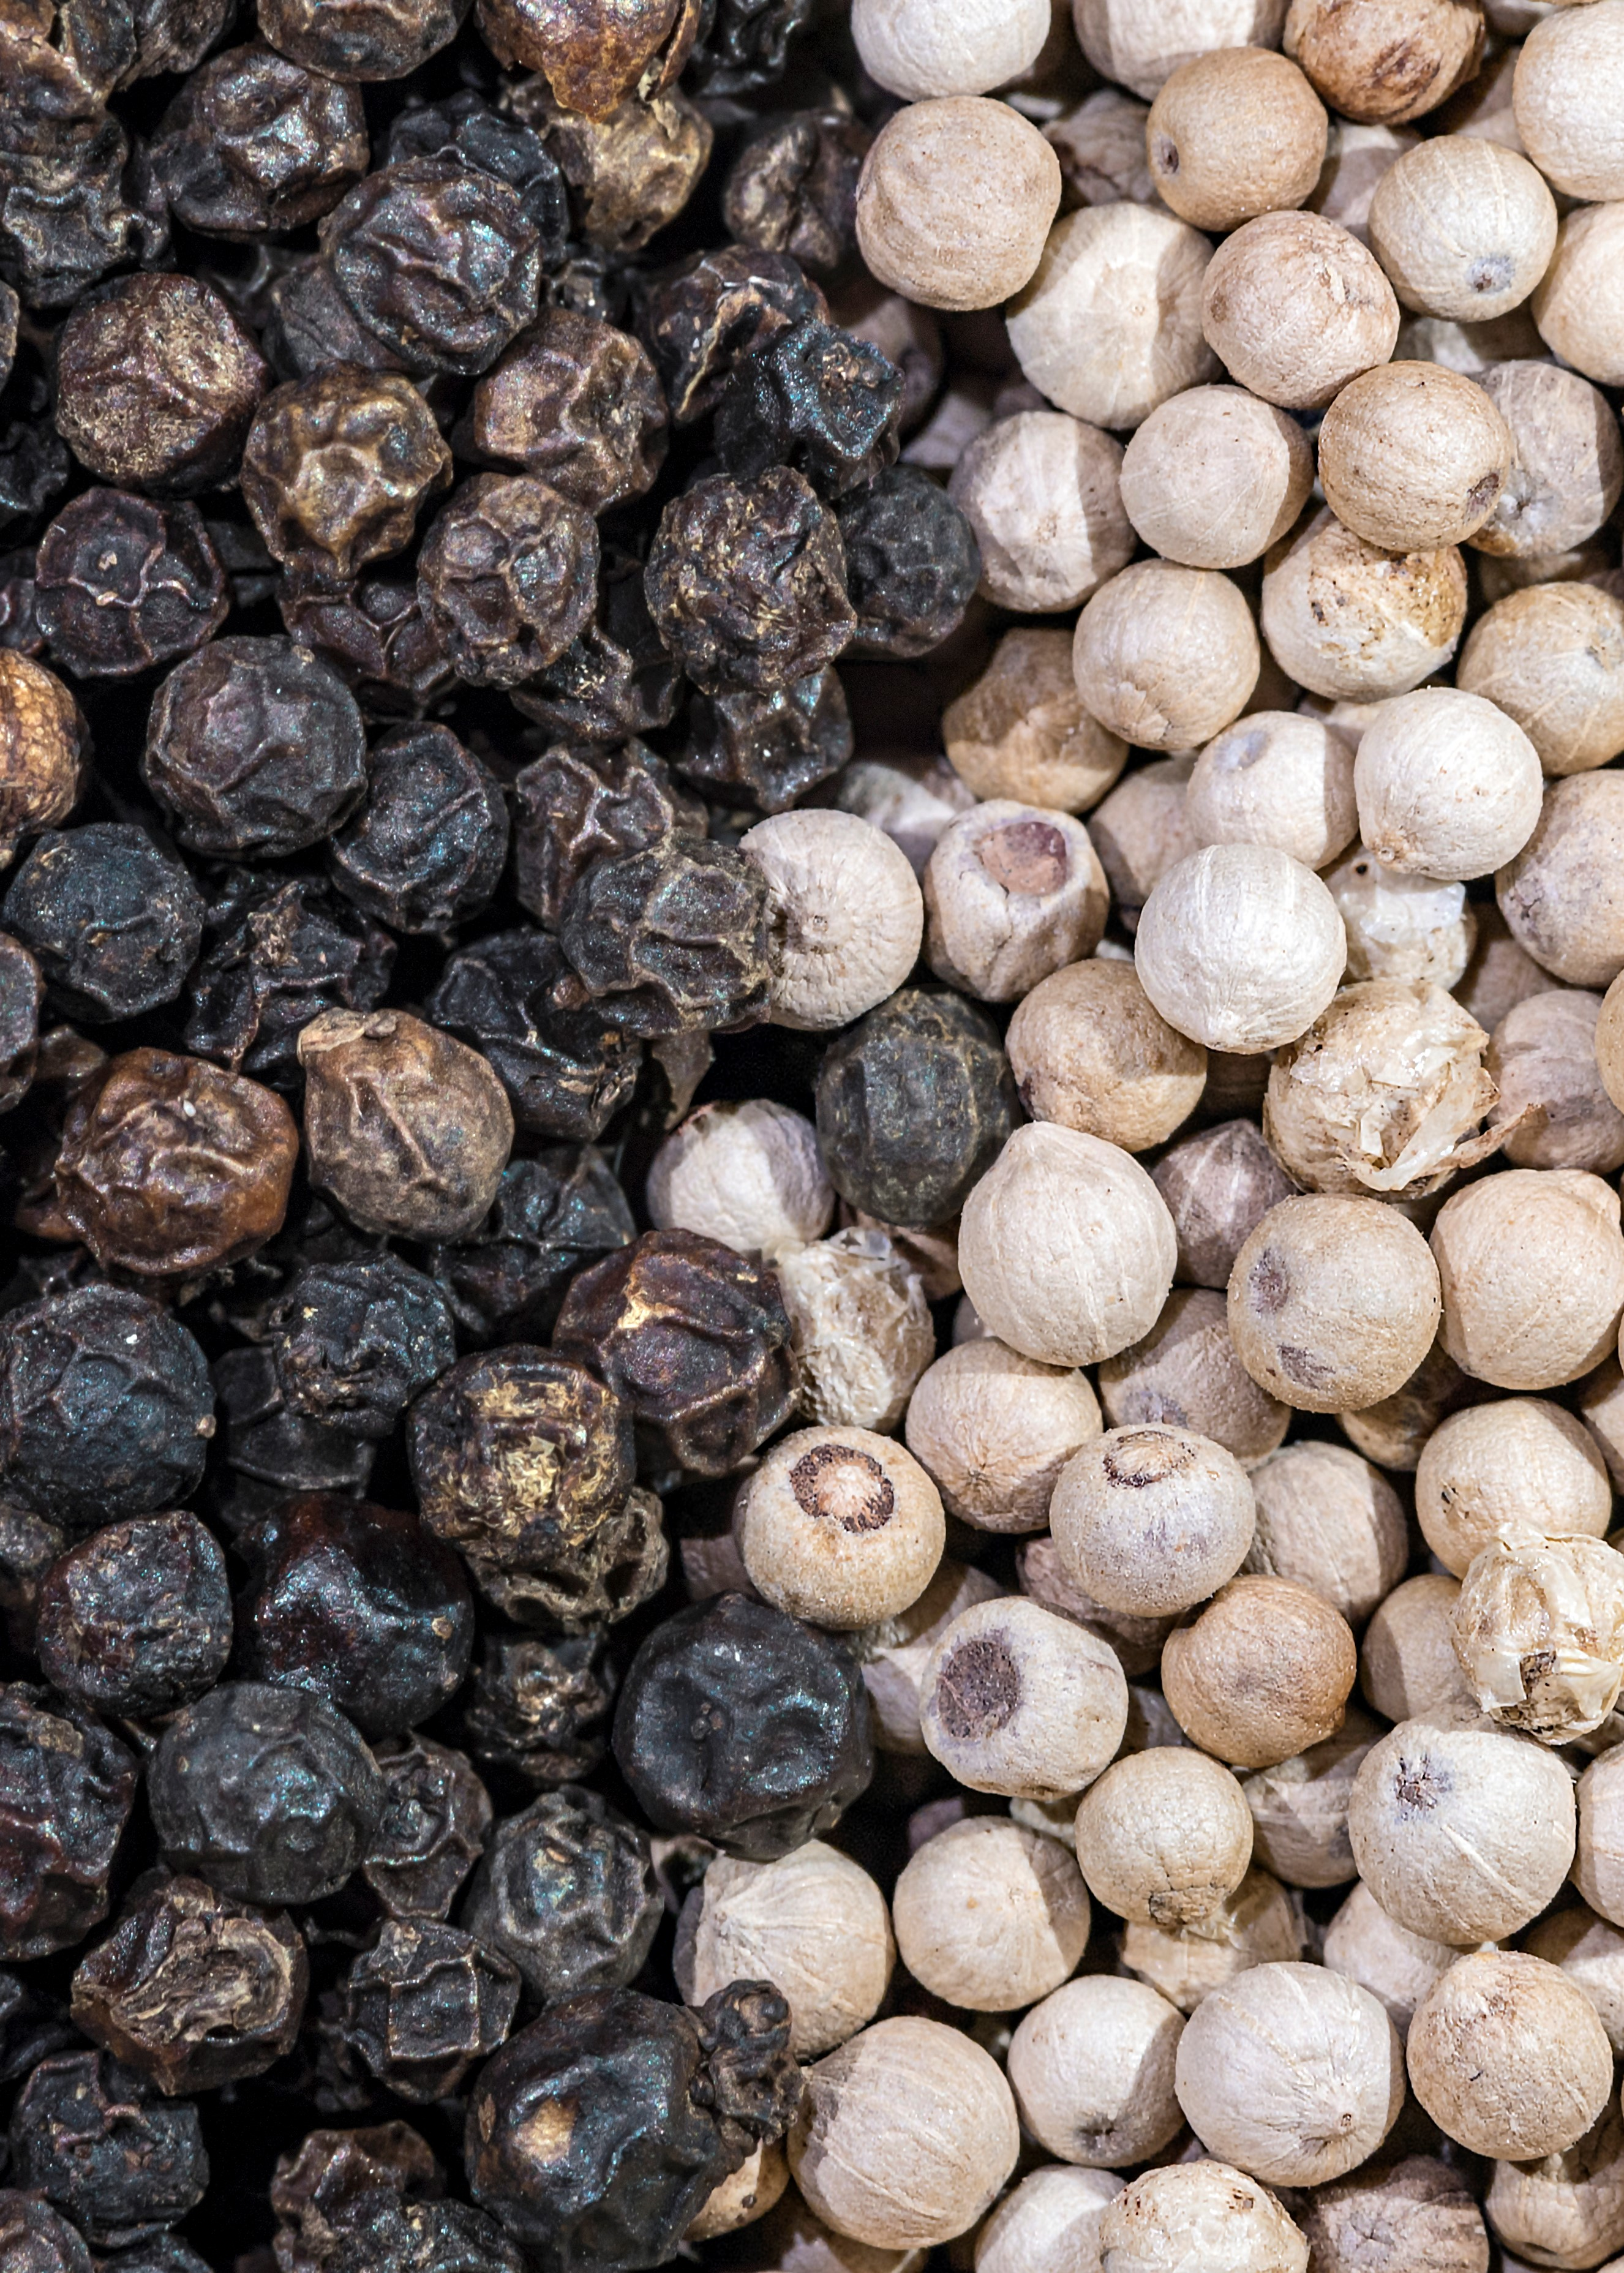
\includegraphics[width=\paperwidth,height=\paperheight]{imgs/piper-nigrum.jpg}
%   }%
% }

% Use the following code to add background image on a page:
% \BgThispage
% Some content
% \clearpage

% Linguistic trees
\usepackage[linguistics, edges]{forest}
% Easy extra edges
\forestset{
  % From an "extra parent" to the node:
  edge to'/.style 2 args={% #1 = the extra parent, #2 = the edge style
    tikz+={\path[#2](#1.parent anchor)--(.child anchor);}
  },
  % From an "extra parent" to the node 
  % using the current edge style:
  % (If the )
  edge to/.style={% #1 = the extra parent
    edge to'/.expanded={\unexpanded{#1}}{\forestoption{edge}},
  },
  % From the node to an "extra child":
  edge from'/.style 2 args={% #1 = the extra child, #2 = the edge style
    tikz+={\path[#2](.parent anchor)--(#1.child anchor);}
  },
  % From the node to an "extra child" 
  % using the current edge style (of the extra child):
  edge from/.style={% #1 = the extra child
    edge from'/.process=_O{#1}{#1.edge},
  },
}
% The "extra parent/child" may be given as a relative node name. 
% So in the example below, we could replace
% "edge to=MG" with "edge to=!uus" (uus=up,up,sibling).
% Also: position a node between siblings: before computing xy={s/.average={s}{siblings}}, 

% Linguistics
\usepackage{tipa}
\usepackage{expex}
% \lingset{everyglpreamble=, everygla=\it, everyglb=\small, belowglpreambleskip=-0.5ex, aboveglftskip=-0.5ex}

% Colors
\definecolor{vanilla}{HTML}{F3E5AB}
\definecolor{cinnamon}{HTML}{D2691E}

% Define a color sample shape
\newcommand{\sample}[1]{
\begin{tikzpicture}[x=1ex,y=1ex]
\filldraw[#1] (0,0) rectangle (2.5,1);
\end{tikzpicture}}

% Scientific names of species, taxons
\newcommand{\taxon}[1]{\emph{#1}}
\newcommand{\taxonn}[2]{\emph{#1} \footnotesize #2\normalsize}

% \usepackage{silence}
% \WarningFilter{biblatex}{File 'arabic-apa.lbx'}

% Thesis metadata
\usepackage[en-US]{datetime2}
\title{Mapping the Language of Spices}
\newcommand{\subtitle}{A corpus-based, philological study on the words of the spice domain}
\author{G{\'{a}}bor Parti}
\DTMsavedate{ini}{2022-08-01}  % date of creation
\DTMsavedate{rev}{2022-09-01}  % date of revision
\date{\DTMusedate{ini}}
\def\degree{Doctor of Philosophy}
\def\university{The Hong Kong Polytechnic University}
\def\department{Department of Chinese and Bilingual Studies}
\hypersetup{
    pdftitle=\thetitle,
    pdfauthor=\theauthor,
    pdfsubject={},
    pdfkeywords={}}



\begin{document} 

\frontmatter

\hypersetup{pageanchor=false}
% \begin{titlepage}
%     \centering

%     \rule{\textwidth}{1.6pt}\vspace*{-\baselineskip}\vspace*{2pt}
%     \rule{\textwidth}{0.4pt}\par
%     {\huge\bfseries\MakeUppercase{\thetitle}\par}
% 	\rule{\textwidth}{0.4pt}\vspace*{-\baselineskip}\vspace{3.2pt}
% 	\rule{\textwidth}{1.6pt}\par
%     \vspace{4em}
%     {\Large by\par}
%     \vspace{2em}
%     {\LARGE\bfseries\MakeUppercase{\theauthor}\par}
%     \vspace{6em}
%     {\large\degree\par}
%     \vspace{4em}
%     {\large\textit{\university}\par}
%     \vspace{2em}
%     \def\svgwidth{1.5in}
%     % \input{univ.pdf_tex}\par
%     
\includegraphics[width=0.33\linewidth]{imgs/logos/univ.pdf}\par
%     \vfill

%     \makeatletter
%     {\Large\@dtm@ini@year\par}
%     \vspace{1em}
%     Copyright \copyright\ \theauthor, \@dtm@ini@year.
%     All rights reserved.
%     \makeatother
% \end{titlepage}

%==============================================================

\begin{titlepage}
    \raggedright
    \hfill
    \vfill
    {\LARGE\textsc{\thetitle}\par}
    {\Large\textsc{\subtitle}\par}
    \rule{\textwidth}{.5pt}\par
    {\Large\textsc{\theauthor}\par}
    \vspace{5em}
    {\large\itshape\degree\par}
    \vspace{0.5em}
    {\large\itshape\university\par}
    \vfill
    \makeatletter
    \centering
    {\Large---\textsc{Initial Submission for Examination Purpose}---\par}
    \vspace{1.5em}
    {⸙ }
    {\Large\@dtm@ini@year\par}
    % \vspace{0.5em}
    % Copyright \copyright\ \theauthor, \@dtm@ini@year.
    % All rights reserved.
    \makeatother
\end{titlepage}

\thispagestyle{empty}
\vspace*{\fill}
\begin{center}
{\small Typeset in Brill Typeface version 4.0 with \hologo{LuaLaTeX} on \DTMusedate{ini} (Revised on \DTMusedate{rev}).\par}
\vspace{0.5ex}
\makeatletter
{\small \copyright\ \theauthor~\orcid{0000-0003-2042-4655},  \@dtm@ini@year. All rights reserved. \\ ⚓ Hong Kong} 
\makeatother
\vspace{-2.75ex}
\end{center}


% \begin{titlepage}
%     \centering
%     {\large\university\par}
%     \vspace{0.5em}
%     {\large\department\par}
%     \vfill
%     {\parbox[b]{0.8\textwidth}{\centering\Huge\textsc{\thetitle}}\par}
%     \vspace{0.5em}
%     {\large\signaturesymbol\par}
%     \vspace{0.75em}    
%     {\parbox[b]{0.8\textwidth}{\centering\huge\textsc{\subtitle}}\par}
%     \vspace{2.5em}
%     {\textit{by}\par}
%     {\LARGE\textsc{\theauthor}\par}
%     \vfill
%     
\includegraphics[width=0.25\linewidth]{imgs/logos/univ.pdf}\par
%     \vfill
%     {\large\itshape
%         A thesis submitted in partial fulfillment\par
%         of the requirements for the degree of\par
%         \degree}
%     \vfill
%     % {\Large---\textsc{Initial Submission for Examination Purpose}---\vfill\par}
%     \makeatletter
%     {\large\DTMenglishmonthname{\@dtm@ini@month}, \@dtm@ini@year}
%     \makeatother
% \end{titlepage}

\begin{titlepage}
    \centering
    {\large\university\par}
    \vspace{0.5em}
    {\large\department\par}
    \vfill
    {\parbox[b]{0.8\textwidth}{\centering\Huge\textsc{\thetitle}}\par}
    \vspace{0.5em}
    {\large~\par}
    \vspace{0.75em}    
    {\parbox[b]{0.8\textwidth}{\centering\huge\textsc{\subtitle}}\par}
    \vspace{2.5em}
    % {\textit{by}\par}
    {\LARGE\textsc{\theauthor}\par}
    % \vfill
    % 
\includegraphics[width=0.25\linewidth]{imgs/logos/univ.pdf}\par
    \vfill
    {\large\itshape
        A thesis submitted in partial fulfillment\par
        of the requirements for the degree of\par
        Doctor of Philosophy\par}
    % \vspace{2.5em}
    \vfill
    % {\Large---\textsc{Initial Submission for Examination Purpose}---\vfill\par}
    \makeatletter
    {\large\DTMenglishmonthname{\@dtm@ini@month}, \@dtm@ini@year}
    \makeatother
\end{titlepage}
\hypersetup{pageanchor=true}

\chapter*{Certificate of originality}
\label{ch:certificate}
\markboth{\nameref*{ch:certificate}}{\nameref*{ch:certificate}}

I hereby declare that this thesis is my own work and that, to the best
of my knowledge and belief, it reproduces no material previously
published or written, nor material that has been accepted for the award
of any other degree or diploma, except where due acknowledgment has
been made in the text.

\vfill

\begin{flushright}
    \begingroup
        \renewcommand{\arraystretch}{1.5}
        \newcommand*{\hrulefilled}[1]{\hrulefill\vskip-1.8em\makebox[\linewidth]{\textit{#1}}}
        \begin{tabular}{p{.4\linewidth}l}
            \hrulefill                  & (Signed)\\
            \hrulefilled{\theauthor}    & (Name of Student)\\
        \end{tabular}
    \endgroup
\end{flushright}

% \chapter*{Dedication}
\label{ch:dedication}
\markboth{\nameref*{ch:dedication}}{\nameref*{ch:dedication}}

This dissertation is dedicated to teachers, professors, educators.
\chapter*{Abstract}
\label{ch:abstract}
\addcontentsline{toc}{chapter}{\nameref*{ch:abstract}}
\markboth{\nameref*{ch:abstract}}{\nameref*{ch:abstract}}

% Abstract (consisting of a summary of the work done with 200-500 words)

% 2 Abstract
% Describes what happened during the research.
% What is the reason for writing the thesis?
% What are the current approaches and gaps in the literature?
% What are your research question(s) and aims?
% Which methodology have you used?
% What are the main findings?
% What are the main conclusions and implications?

% \leftskip1in\relax
% \rightskip1in\relax

The majority of existing literature on spices is found in the areas of gastronomy, botany, and history. This study investigates spices on a linguistic level and aims to be a comprehensive linguistic account on the items of the spice trade. Some of these dried plant matter were highly desired at certain points in history, due to their attractive aroma and medicinal value, thus they were ideal products of trade early on. Cultural contact and exchange, and the introduction of new cultural items begets situations of language contact and linguistic acculturation, and so in the case of spices, we not only have a set of items that traveled around the world, but also a set of names. This domain is very rich in loanwords and \textit{Wanderwörter}, but also supplies us with a myriad of cases where spice names are conventional innovations. To make it more interesting, the thesis compares English, Arabic, and Chinese, languages that represent major powers in the spice trade at different times. After selecting a set of 24 spices, I have collected data on their names and related etymologies, and introduced 6 of them in detail regarding their identity, botany, history, spread, and names. The thesis has two main parts. Part one represents the geographic and linguistic diffusion of spices and their names. Basically, I track and explain word origins and subsequent spread by tracing the materials and the propagation of the accompanying \textit{Wanderwort}. This part relies on philological literature, and tools from historical linguistics, such as etymological research, as well as geospatial visualizations. Part two examines the language of spices, referring to the terminology and nomenclature related to the spice domain from linguistic-cognitive perspectives. Focusing on the structure and components of 360 collected spice names, it is a systematic investigation on how humans name spices: what are the mechanism and motivations behind the naming principles, and how this possibly relates to the salient sensory features of the products (strong gustatory, olfactory, or visual stimuli). Conclusions are made on the connections between the physical properties of the spices, their patterns of diffusion, and the prototypical spices and their effect of naming principles. Besides being a novel and original approach to research and categorize spices from a linguistic point of view, this study offers new insights to our knowledge about wandering loanwords, and the effect of the highly sensory nature of spices in the naming process when adopted by a community. It is also intended to be a basis for a useful working database for future research, and aims to dispel some of the chaos and confusion surrounding spice names.

\leftskip0cm\relax
\rightskip0cm\relax
% \chapter*{Publications}
\label{ch:publication}
\addcontentsline{toc}{chapter}{\nameref*{ch:publication}}
\markboth{\nameref*{ch:publication}}{\nameref*{ch:publication}}

Publications arising from the thesis (optional; and should be presented in alphabetical order of the first author using the reference citation format for academic journal papers, book chapters, conference papers, research reports/working papers and books/research monographs, or in an internationally accepted format used by the discipline in which the study lies.)
\chapter*{Acknowledgments}
\label{ch:acknowledgments}
\addcontentsline{toc}{chapter}{\nameref*{ch:acknowledgments}}
\markboth{\nameref*{ch:acknowledgments}}{\nameref*{ch:acknowledgments}}

% 1 Acknowledgments
% Recognize those who contributed to your research.
% How did your supervisors and others contribute?
% Do you need to thank those who provided help during data-collection, including participants?
% Did anyone provide pastoral support, including friends and family?
% Did you have any funding bodies?
% Were any professionals involved, including typists, transcribers, or proofreaders?

First, I would like to thank my supervisor Prof. Chu-Ren Huang for his guidance and all the support and kindness he gave me in these three years, ever since my first email. He not only believed in my topic, but he taught me new ways to think about words, meanings, concepts, and language. I would also like to thank PolyU and the department of Chinese and Bilingual Studies (CBS) who equipped me with a workspace and never-ending answers to all my questions regarding the PhD program. I want to highlight the Pao Yue-Kong Library and its staff supplying us with space, workshops, a wide range of books and materials, who can grant requests so promptly whenever we suggest a purchase; truly helpful. I also cannot leave out the lovely people who run the LibCafé. Next, I would like to express my gratitude to my two external examiners, Prof. Victor H. Mair and Prof. Baoya Chen, who took their time to read this work, gave invaluable comments, and encouraged me to continue on this path. I must also thank the Research Grants Council (RGC) of the University Grants Committee (UGC) of Hong Kong, who funded this PhD program under the Hong Kong Ph.D. Fellowship Scheme (HKPFS, ref. no. PF18-22990). Lastly, I want to thank the people of Hong Kong, who welcomed me to their intriguing city.

As probably this is the end of my \textit{official} journey as a student---\textit{official} because in reality we all know this path never ends---I want to thank all my teachers and professors from whom I learned so much throughout these years at my alma mater, the Eötvös Loránd University (ELTE) in Budapest. Especially ?? the list is so long. I am grateful for all the knowledge and insight I received from everyone.

Most importantly, I want to thank my friends here who helped me all the way, especially Yun and Andreas, and of course my parents back home, who have always supported this life of study with patience.

% Tamás Iványi, Zoltán Szombathy, Sándor Fodor, Dóra Zsom, István Ormos, István Hajnal, El-Adly Saber, Rashid Daher, Ágnes Birtalan, Mária Négyesi, Csaba Dezső, Rama Yadav, 

% Beatrix Mecsi, Mózes Csoma, Fendler Károly, Kim Bo-Guk, Valéria Simon, András Bereczki, Kata Torma, Péri Benedek, Orsolya Saraç, Alexa Péter

% \chapter{Quotes}

\epigraph{Maths is hell}{Tom, 2021}

\epigraph{Pepper is the bride around which everybody dances.}{Jacob Hustaert, 1664, a Dutch East India Company Governor of Sri Lanka}

\epigraph{Pepper is small in quantity and great in virtue.}{Plato}

\epigraph{Thus to the Eastern wealth through storms we go, 
But now, the Cape once doub’led, fear no more;
A constant trade-wind will securely blow,
And gently lay us on the spicy shore.}{Annus Mirabilis, John Dryden}

One Dutch ditty of the day went:
Wherever profit leads us,
To every sea and shore,
For love of gain,
The wide world’s harbours we explore.


\epigraph{He who controls the spice, controls the universe}{Dune?}

\epigraph{What are little girls made of? Sugar and spice and all things nice}{English nursery rhyme} %%%%%%%%%%%%%%%%

\cleardoublepage
\tableofcontents
\markboth{\contentsname}{\contentsname}

\cleardoublepage
\listoffigures
\markboth{\listfigurename}{\listfigurename}

\cleardoublepage
\listoftables
\markboth{\listtablename}{\listtablename}

% \cleardoublepage
% \printunsrtglossary[type=main, title={Glossary}]
% \printunsrtglossary[type=acronym, title={List of Abbreviations}]
% \printunsrtglossary[type=symbols, title={Symbols and Notation}] 
% \printunsrtglossary[type=primary, title={Primary sources}, style=index]

\cleardoublepage % Not working on Overleaf!
\printglossary 
\printglossary[type=acronym]
\printunsrtglossary[type=symbols, title={Symbols and Notation}]

% % To compile locally, download the project source code, command in folder: <latexmk> or <lualatex thesis> (assuming you have LaTeX/MiKTeX, https://www.latex-project.org/get/)

% \ifdraft{
%     \cleardoublepage
%     \phantomsection
%     \todototoc
%     \listoftodos}{}

\mainmatter

% \chapter{Test}
\label{sec:test}

\lettrine[lines=4, lraise=0.1, nindent=0em, slope=-.5em]%
{\textcolor{PolyU}{V}}{oici} un exemple... 

\lettrine[lines=6, slope=0.5em, findent=-1em]%
{A}{} nearly full list of features and tools are tested here, from typesetting to citations. 

\blindtext[1]

\bigskip



1234567890 .,:;?!@ \# \$ \% \^ \& \* () [] \{\} <> || - + = * ``Common'' ligatures ff, fi, and ffi, ``rare'' ones are st, ct, is. \textsc{smallcaps} and \textss{superscript}. \nth{1} \nth{2} \nth{3} \nth{4} \nth{19} century \BC, \AD. (if you don't see \emph{small capitals} \textsc{here}, the font does not have them).

\noindent{\color{black}\rule{\linewidth}{0.2mm}} 

\section{Section}

\subsection{Subsection}

\subsubsection{Subsubsection} 

A `subsubsection' will not appear in the TOC. \marginpar{TOC means Table of Contents}


\noindent{\color{black}\rule{0.25\linewidth}{0.2mm}} this is baseline

\noindent{\color{black}\rule[0.5ex]{0.25\linewidth}{0.2mm}} this is half raised

\noindent{\color{black}\rule[1ex]{0.25\linewidth}{0.2mm}} this is raised

\noindent{\color{black}\rule[1.5ex]{0.25\linewidth}{0.2mm}} this is raised above

\section{Typesetting}

\begin{table}
\begin{tabular}{@{}lll@{}}
\toprule
Normal      & Sphinx of black quartz, judge my missing vow forever. \\
Bold        & \textbf{Sphinx of black quartz, judge my missing vow forever.} \\
Italic      & \textit{Sphinx of black quartz, judge my missing vow forever.} \\
Bold-Italic & \textbf{\textit{Sphinx of black quartz, judge my missing vow forever.}} \\
Small caps  & \textsc{Sphinx of black quartz, judge my missing vow forever.} \\
Uppercase   & \uppercase{Sphinx of black quartz, judge my missing vow for} \\
Sans serif  & \textsf{Sphinx of black quartz, judge my missing vow forever.} \\
Mono        & \texttt{Sphinx of black quartz, judge my missing vow forever.} \\ \bottomrule
\end{tabular}
\caption{Different font styles of the typeface.}
\end{table}

\bigskip

Various scripts and languages:\marginpar{This is a marginpar, and it should go on the outer margin automatically.}

Hungarian: köszönöm szépen \textit{köszönöm szépen} \textbf{köszönöm szépen}

Greek: ευχαριστώ \textit{ευχαριστώ} \textbf{ευχαριστώ}

Russian: спасибо \textit{спасибо} \textbf{спасибо}

Chinese, Simplified: 汉字:艹草,谢谢。 \textbf{汉字:艹草,谢谢。}

Chinese, Traditional: 漢字:艸草,謝謝。 \textbf{漢字:艸草,謝謝。}

Japanese: ありがとうございました \textbf{ありがとうございました }

Korean: 감사합니다 \textbf{감사합니다}

\textnormal
Devanagari: धन्यवाद \textbf{धन्यवाद}

Arabic: شكرا جزيلا  \textit{شكرا جزيلا} \textbf{شكرا جزيلا}

\textnormal
Hebrew: תֹהוּ וָבֹהוּ \textbf{תֹהוּ וָבֹהוּ} 

Tibetan: {\tibetanfont{ཐུགས་རྗེ་ཆེ་།} \textbf{ཐུགས་རྗེ་ཆེ་།}}

Javanese: {\javanesefont{ꦩꦠꦸꦂꦤꦸꦮꦸꦤ꧀} \textbf{ꦩꦠꦸꦂꦤꦸꦮꦸꦤ꧀}}

Tamil: {\tamilfont{மிக்க நன்றி} \textbf{மிக்க நன்றி}}

Sumero-Akkadian Cuneform: {\cuneifont{\GA \NU \UU \UM \Leftarrow \GI}}



\section{Bidirectional scritps}

Arabic and Hebrew in English paragraphs, in mixed environments:

ما هو \foreignlanguage{english}{differentiation}? 

What is ما هو in Arabic?
\medskip
\textnormal
\noindent Most Arabic speakers consider the two varieties to be two registers
of one language, although the two registers can be referred to in
Arabic as فصحى العصر \textit{fuṣḥā l-ʻaṣr} Modern Standard Arabic (MSA) and
فصحى التراث \textit{fuṣḥā t-turāth} Classical Arabic (CA). ʿArab\={i}.

\medskip

The first line of the Bible is בְּרֵאשִׁית בָּרָא אֱלֹהִים אֵת הַשָּׁמַיִם וְאֵת הָאָרֶץ (Genesis 1:1).

% Don't use these
% \selectlanguage{arabic}
% مكانة عائلته الاجتماعية مكنته من الدراسة على يد أفضل المدرسين في المغرب العربي. تلقى علم التربية الإسلامية التقليدية، ودرس القرآن الكريم الذي كان يحفظه عن ظهر قلب، واللسانيات العربية، وأساس فهم القرآن، الحديث، الشريعة (القانون) والفقه علم التاريخ.
% \selectlanguage{english}

% For inline usage: \foreignlanguage{hebrew}{תַּבְלִין}




\section{Acronyms, terms, and indexing}

\begin{wrapfigure}{o}{0.25\textwidth}
  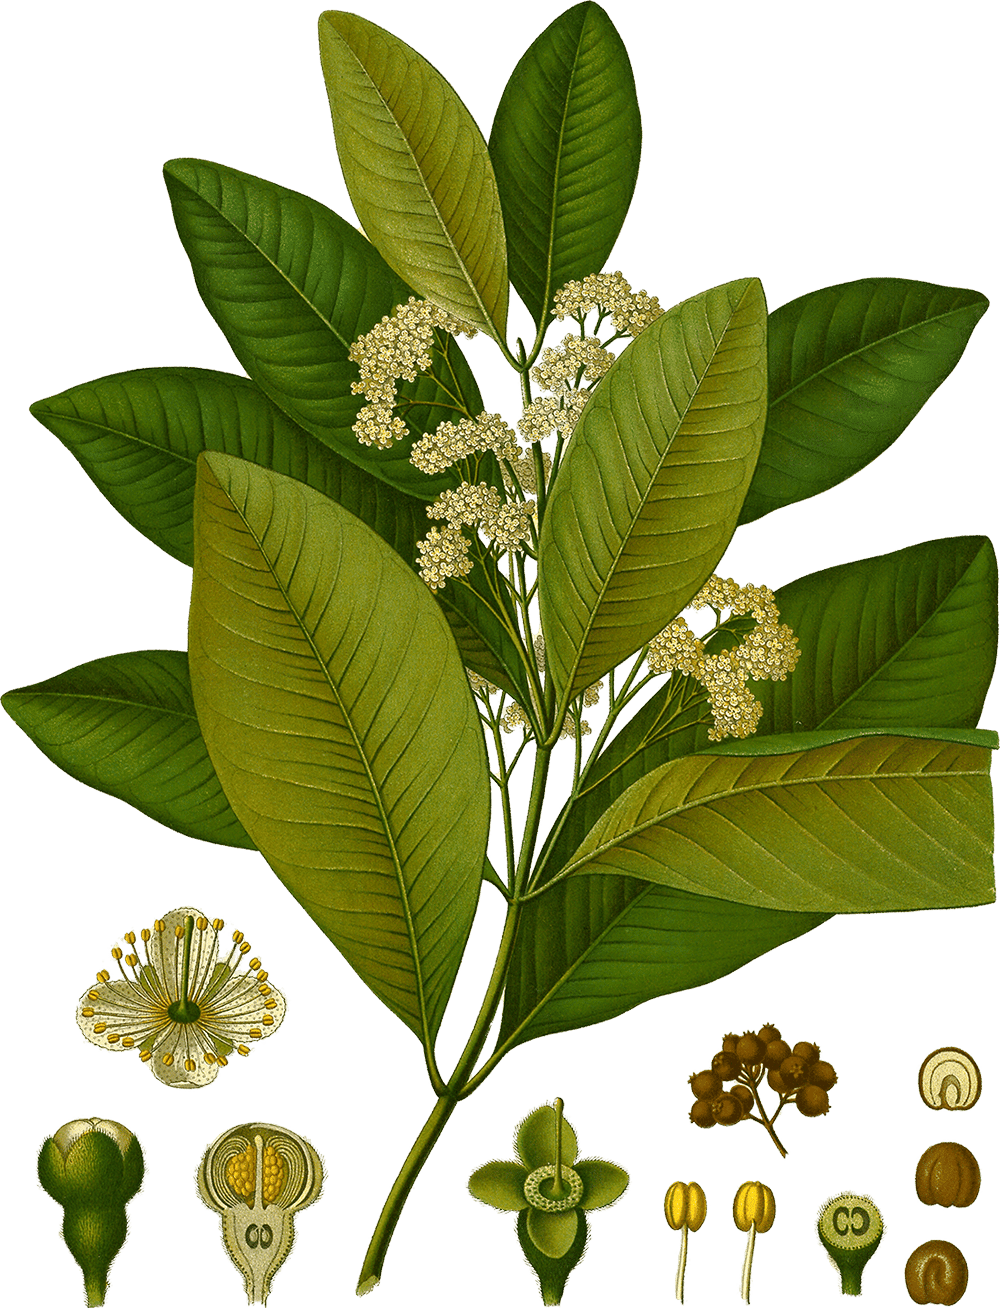
\includegraphics[width=0.25\textwidth]{imgs/kohler/allspice_kohler_min.png}
  \caption{Allspice}
\end{wrapfigure}

The \gls{latex} typesetting markup language is specially suitable 
for documents that are annoying to make.

Glossaries like the above have to be set in the glossary.tex, and then called:
This is the first time \gls{POWO} appears, and the second time \gls{POWO} appears. For plural and capital varieties:
\gls{cultigen} and \glspl{cultigen}; \Gls{taxon} and \Glspl{taxon}

\bigskip

The index one\index{one} is here and two\index{two} is here. There is also index for tables \index{three|tb}, figures\index{four|fg}, and footnotes\index{five|fn}.
Also, there is grouped indexing possible for things like black pepper\index{pepper!black}, white pepper\index{pepper!white}, and green pepper\index{pepper!green}. 

WARNING: The index on Overleaf only prints on your pdf if you run it for the first time/clear the cache. I don't know why, currently unsolved.

\section{Citations}

Citation examples, such as \parencite[99]{huang_routledge_2019} and \textcite{huang_routledge_2019}. 
Multi-volume citing also available, \pvolcite[]{9}[99]{bearman_encyclopaedia_1960} \& \tvolcite[]{9}[99]{bearman_encyclopaedia_1960}.

\section{Environments}

\begin{note}
    This is a note.
\end{note}

\begin{equation}
    \label{eq:1}
    x^2  = 1
\end{equation}

And this was an equation. In Equation \ref{eq:1} we have~$\sqrt{\log n}$.

\ex
\begingl
\gla\rightcomment{Hungarian (Finno-Ugric, \emph{reference})}Ez egy példám.//
\glb This a example.my//
\glft ``This is an example of mine.''//
\endgl
\xe




\begin{etymology}\label{etym:pepper}
\raggedright
English \textit{pepper}
< Middle English \textit{peper}
< Old English \textit{pipor}
< West Germanic \textit{*piper}
< Latin \textit{piper} `black pepper, long pepper'
< Ancient Greek \textit{péperi} `pepper'
< Pahlavi
< Middle Indo-Aryan \textit{pipparī} `long pepper'
< Sanskrit \textit{pippalī} `berry, peppercorn', \textit{pippali} `long pepper'
\end{etymology}

\begin{spice}
\textsc{Black pepper} \hfill \href{https://powo.science.kew.org/taxon/682369-1}{POWO} \\ 
\textbf{English:} \textit{pepper; black pepper}. \textbf{Hungarian:} \textit{bors, fekete bors}. \textbf{Arabic:} فلفل، فلفل أسود \textit{filfil/fulful, filfil/fulful aswad}. \textbf{Chinese:} 胡椒, 黑胡椒 \textit{hújiāo, hēihújiāo} [nan]. \\
\noindent{\color{black}\rule[0.5ex]{\linewidth}{.5pt}}
\vspace*{-2.5\multicolsep}
\begin{multicols}{2}
\begin{tabular}{@{}ll@{}}
Plant species: & \textit{Piper nigrum L.} \\
Family: & \textit{Piperaceae} \\
Region of oigin: & South India \\
Plant part(s) used: & fruit; unripe fruit \\
Color: & black; white; green \\
\end{tabular}
\end{multicols}
\end{spice}

This is a ref for Etymology \ref{etym:pepper} and then this is a cleverref for \Cref{sec:test}.

\blindtext

\poemtitle{Un poem de la lalala}
\settowidth{\versewidth}{Fallait-il que je ecteffst vous aimasse,}
\begin{verse}[\versewidth]
 Fallait-il que je ecteffst vous aimasse, \\
 Que vous me désespérassiez, \\
 Et qu’en vain je m’opiniâtrasse, \\
 Et que je vous idolâtrasse \\
 Pour que vous m’a\lgSS a\lgSS ina\lgSS iez ! \\
\end{verse}
\attrib{Je ne sai qui}

\begin{quote}
\textsc{``Another remedy which the Goddess Isis prepared for the God Ra to drive out the pains that are in his head!}

\smallskip
Berry-of-the-Coriander---I\\
Berry-of-the-Poppy-plant---I\\
Wormwood---I\\
Berry-of-the-sames-plant---I\\
Berry-of-the-Juniper-plant---I\\
Honey---I
\smallskip

Make into one, mix with Honey, and smear therewith in order to make him well forthwith. When this remedy is used by him against all illnesses in the head and all sufferings and evils of any sort, he will instantly become well.'' \textcite[40]{bryan_papyrus_1930}
\end{quote}

\begin{figure}[!hbt]
    \centering
    \subfloat{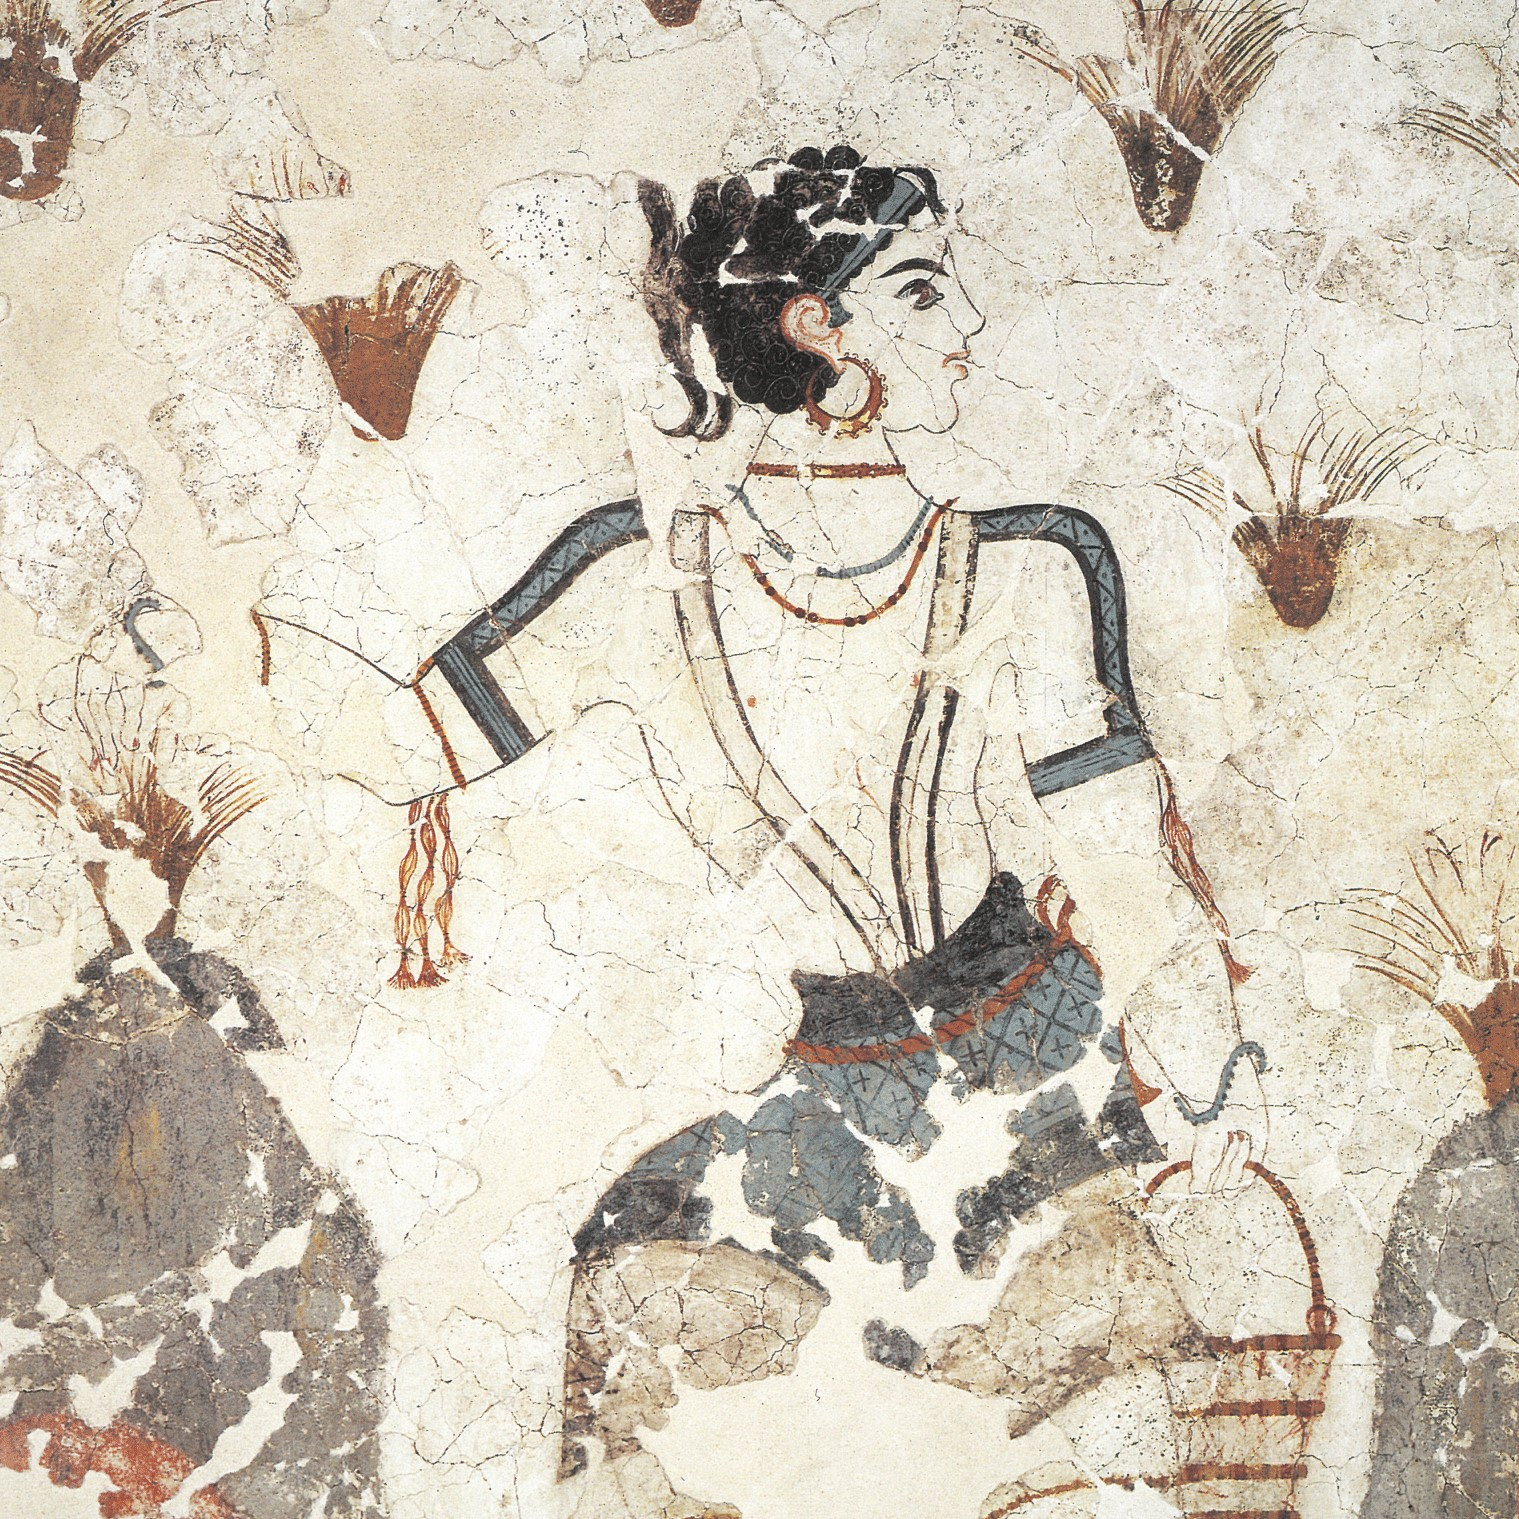
\includegraphics[width=0.482\linewidth]{imgs/saffron_gatherers_l.jpg}}
    \hfill
    \subfloat{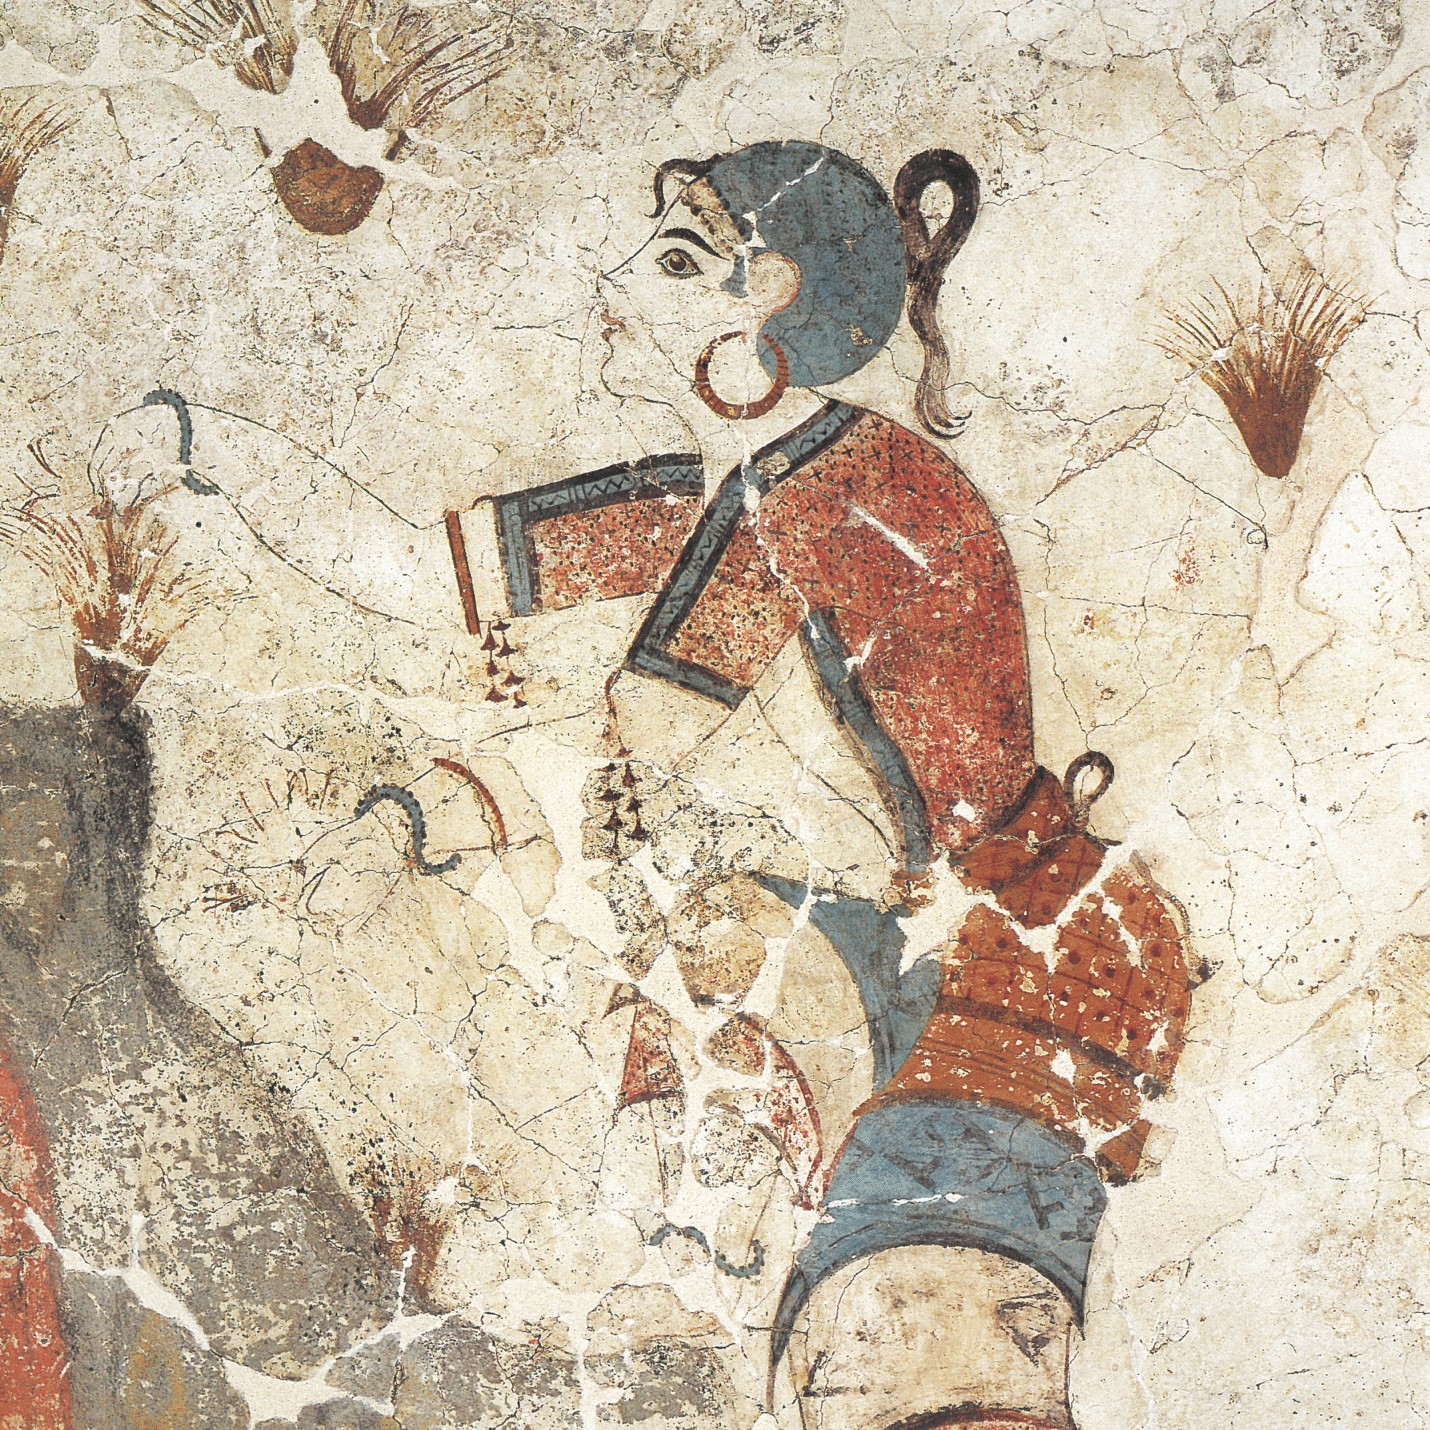
\includegraphics[width=0.482\linewidth]{imgs/saffron_gatherers_r.jpg}}
    \caption{Saffron-gatherers. Details from the mural on the east wall in room 3a, first floor, at Xeste 3 site, Akrotiri at Thera \parencite[152]{doumas_wall-paintings_1992}.}
    \label{fig:saffron_gatherers}
\end{figure}

\epigraph{By convention sweet and by convention bitter, by convention hot, by convention cold, by convention color; but in reality atoms and void.}{Democritus, \nth{3} century BC\\(DK 68B9, trans. Taylor 1999a)}

% \epigraph{We shall not cease from exploration. And the end of all our exploring. Will be to arrive where we started. And know the place for the first time.}{T. S. Eliot}

\section{IPA}

\textipa{[ðIsIzsAmaIpeI]}, \textipa{[Its\*rilijizitutaIp]} as in: ``This is some IPA, it's really easy to type.''

\begin{longtable}{p{0.15\textwidth}p{0.3\textwidth}p{0.3\textwidth}}
  \toprule
  \endfirsthead
  \toprule
  \endhead
  \bottomrule
  \endfoot
  \bottomrule
  \endlastfoot
  Consonant & Onset & Coda\tabularnewline

  \midrule p & pun.za (claw) & \textipa{k\super hap.Ra} (old man)\tabularnewline

  b & \textipa{bO\|[d\super h} (bull) & \textipa{Seb.Ra} (dull)\tabularnewline

  \textipa{b\super h} & \textipa{b\super he\:d} (sheep) & \tabularnewline

  m & \textipa{mE} (me) & \textipa{amb} (mango)\tabularnewline

  f & ful (flower) & \tabularnewline

  \textipa{V} & \textipa{Vi\|[d.jaR.\|[t\super hi} & \textipa{RoVa}
  (injury)\tabularnewline

  \textipa{\|[t} & \textipa{\|[tu} (you) & \textipa{mO\|[t}
  (don't)\tabularnewline

  \textipa{\|[d} & \textipa{\|[deS} (many) & \textipa{swa\|[d}\tabularnewline

  \textipa{\|[t\super h} & \textipa{\|[t\super he\:n.\:di} (cold) &
  \textipa{hO\|[t\super h} (hand)\tabularnewline

  \textipa{\|[d\super h} & \textipa{\|[d\super hus.ki} (down) &
  \textipa{bO\|[d\super h} (bull)\tabularnewline

  \textipa{\t*{ts}} & \textipa{\t*{ts}Ol.\:na} (to walk) & \textipa{so\t*{ts}}
  (think)\tabularnewline

  \textipa{\t*{ts}\super h} & \textipa{\t*{ts}\super hekke} (fast) &
  \tabularnewline

  \textipa{\t*{dz}} & \textipa{\t*{dz}a.\:na} (to go) & \tabularnewline

  \textipa{n} & \textipa{n@i} (no) & \textipa{an.\|[dRe} (inside)\tabularnewline

  \textipa{R} & \textipa{me.Ri} (my) & \textipa{g\super hOR}\tabularnewline

  \textipa{s} & \textipa{sen.\|[tRi} (orange colour) & \textipa{hOs\:na} (to
  laugh)\tabularnewline

  \textipa{z} & \textipa{ze\:d} (root) & \textipa{Roz} (everyday)\tabularnewline

  \textipa{l} & \textipa{lOm.ma} (long) & \textipa{kal}
  (yesterday)\tabularnewline

  \textipa{S} & \textipa{Sob.la} (beautiful) & \textipa{gaS}
  (rain)\tabularnewline

  \textipa{\:t} & \textipa{\:te\:d.\:da} (curved) & \textipa{nO\:t.\:t\super he}
  (gone)\tabularnewline

  \textipa{\:t\super h} & \textipa{\:t\super he\:n\:ra} (cold) &
  \textipa{nO\:t.\:t\super he} (gone)\tabularnewline

  \textipa{\:d} & & \textipa{ne\:d} (near)\tabularnewline

  \textipa{\:d\super h} & & \textipa{pO\:d\super h.na} (to read)\tabularnewline

  \textipa{\:r} & \textipa{pO\:ru} (fell) & \textipa{me\:n.\:r\super h@k}
  (frog)\tabularnewline

  \textipa{\:n} & \textipa{\|[de.\:na} (to give) & \textipa{ku\:n}
  (who)\tabularnewline

  \textipa{\:l} & \textipa{ke\:la} (banana) & \tabularnewline

  \textipa{\t*{tS}} & \textipa{\t*{tS}Ok.ku\|[da} (rotten) & \tabularnewline

  \textipa{\t*{dZ}} & \textipa{\t*{dZ}epuR} (Jaipur) & \tabularnewline

  \textipa{j} & \textipa{ja\|[d} (remember) & \textipa{gaj}
  (abuse)\tabularnewline

  \textipa{k} & \textipa{ki.\:ra} (snake) & \textipa{b\super huk}
  (hunger)\tabularnewline

  \textipa{g} & \textipa{ga} (cow) & \textipa{b\super hEg.\:na} (to
  run)\tabularnewline

  \textipa{k\super h} & \textipa{k\super ha\:na} (to eat) & \textipa{paNk\super
    h} (wing)\tabularnewline

  \textipa{g\super h} & \textipa{g\super hOR} (house) & \tabularnewline

\end{longtable}


\section{Notes}

A thesis submitted for examination purpose should include the words ‘Initial Submission for Examination Purpose’ lettered on the front cover. For details, see: this link \url{https://www.polyu.edu.hk/gs/rpghandbook/ref-regulations-format-thesis/} or the \href{https://www.polyu.edu.hk/gs/rpghandbook/section10/}{RPg Handbook}
Transliteration of Arabic script: \href{https://referenceworks.brillonline.com/pages/help/transliteration-islam}{Brill Online}

\epigraph{We shall not cease from exploration. And the end of all our exploring. Will be to arrive where we started. And know the place for the first time.}{T. S. Eliot}
\index{epighraph}


\epigraph{Maths is hell}{Tom, 2021}

⸙
♰ West Syriac cross
2671 ♱ East Syriac cross
2720 ✠ Maltese cross
2626 ☦ orthodox cross
2627 ☧ khi rho, Christogram
2628 ☨ cross of Lorraine
2629 ☩ cross of Jerusalem
2721 ✡ star of David
262A ☪ star and crescent
262B ☫ Farsi symbol
2638 ☸ wheel of dharma
262C ☬ ādi śakti or khaṇḍā
263D ☽ first quarter moon
263E ☾ last quarter moon
\index[bot]{Cinnamomum verum}

\blindtext

\section{Ideas}

Spices in the Bible

Queen of Sheba in 1 Kings 10:25

Story of Joseph 

Make tree of who taught who in Hungarian orientalists.

Shipnames and their origins: caravel, galleon, dhow, lateen, junk...

Mapping Spice Words - A Linguistic Account of the Spice Trade

Eating the Sinoshphere - Tracing gastronomical loanwords in East Asia

1873 Vienna

Spice names as verbs: pepper, spice, bors, falfala

Vanilla as boredom

Chili pepper vs black pepper RED vs BLACK

marcher d'un pas menu.
se nettoyer la bouche, le dent.
friser, boueler.

berjalan dengan melagak, sombong

contact induced similarities

The (c. 3rd century) Nanzhou yiwu zhi (?????, "Record of Strange Things of the Southern Continent") or Nanfang yiwu zhi (?????, "Record of Strange Things of the South") was written by Wan Zhen (??), and may have been one of Ji Han's sources for his book. 

Spice trade computer game 

serendipity

binomial name

phytonym

\section{Trees}

\section{Example}

best solution:

\begin{forest}
    for tree={align=center,calign=center}
    [paprika\\{English},tier=a,baseline
    [paprika\\{Hungarian},tier=b
    [paprika\\{Serbian-Croatian-Bosnian},tier=c
    [*pĭpĭrĭ\\{Proto-Slavic},tier=d
    [piper\\{Latin},tier=e, before computing xy={s=-s("!u")},
    [péperi\\{Ancient Greek},name=AG,tier=f, edge to=MG,
    [?\\{Pahlavi},tier=g
    [pipparī\\{Middle Indo-Aryan},tier=h
    [pippalī\\{Sanskrit},tier=i]]]]]] 
    [piperi\\{Modern Greek},name=MG]]]]
\end{forest}

\begin{forest}
    for tree={align=center,calign=first}
    [,l sep=0
    [paprika\\\small{English},no edge,tier=a,baseline
    [paprika\\\small{Hungarian},edge={line width=2pt},tier=b
    [pàprika\\\small{Serbian-Croatian-Bosnian},tier=c
    [*pĭpĭrĭ\\\small{Proto-Slavic},tier=d
    [piper\\\small{Latin},tier=e
    [péperi\\\small{Ancient Greek},name=AG,tier=f 
    [?\\\small{Pahlavi},tier=g
    [pipparī\\\small{Middle Indo-Aryan},tier=h
    [pippalī\\\small{Sanskrit},tier=i]]]]]] 
    [piperi\\\small{Modern Greek},edge=dashed,name=MG,edge label={node[midway,below,font=\scriptsize]{influenced}}]
    ]]]
    [1839,no edge,tier=a
    [1569,no edge,tier=b
    [c,no edge,tier=c
    [d,no edge,tier=d
    [e,no edge,tier=e
    [f,no edge,tier=f
    [g,no edge,tier=g
    [h,no edge,tier=h
    [i,no edge,tier=i]]]]]]]]]
    [\href{https://www.etymonline.com/word/paprika\#etymonline_v_3108}{Etymonline},no edge,tier=a
    [source,no edge,tier=b
    [source,no edge,tier=c
    [source,no edge,tier=d
    [source,no edge,tier=e
    [source,no edge,tier=f
    [source,no edge,tier=g
    [source,no edge,tier=h
    [source,no edge,tier=i]]]]]]]]]
    ]  
    \draw[-] (AG.north) to node[above] {\scriptsize{a}} node[below] {\scriptsize{b}} (MG.south);
    \draw[->,dotted] (AG) to[out=east,in=south] (MG);
\end{forest}

\begin{tabular}[t]{ll@{}}
\tikz[baseline]\draw(0,1ex)--(1,1ex); & borrowed\\
\tikz[baseline]\draw[dotted](0,1ex)--(1,1ex); & descended\\
\tikz[baseline]\draw[dashed](0,1ex)--(1,1ex); & influenced\\
\end{tabular}


\begin{folio}{Stuff}\label{folio:pepper}
    \begin{forest}
        for tree={align=center,calign=first}
        [,l sep=0
        [paprika\\\small{English},no edge,tier=a,baseline
        [paprika\\\small{Hungarian},edge={line width=2pt},tier=b
        [pàprika\\\small{Serbian-Croatian-Bosnian},tier=c
        [*pĭpĭrĭ\\\small{Proto-Slavic},tier=d
        [piper\\\small{Latin},tier=e
        [péperi\\\small{Ancient Greek},name=AG,tier=f 
        [?\\\small{Pahlavi},tier=g
        [pipparī\\\small{Middle Indo-Aryan},tier=h
        [pippalī\\\small{Sanskrit},tier=i]]]]]] 
        [piperi\\\small{Modern Greek},edge=dashed,name=MG,edge label={node[midway,below,font=\scriptsize]{influenced}}]]]]
        [1839,no edge,tier=a
        [1569,no edge,tier=b
        [c,no edge,tier=c
        [d,no edge,tier=d
        [e,no edge,tier=e
        [f,no edge,tier=f
        [g,no edge,tier=g
        [h,no edge,tier=h
        [i,no edge,tier=i]]]]]]]]]
        [\href{https://www.etymonline.com/word/paprika\#etymonline_v_3108}{Etymonline},no edge,tier=a
        [source,no edge,tier=b
        [source,no edge,tier=c
        [source,no edge,tier=d
        [source,no edge,tier=e
        [source,no edge,tier=f
        [source,no edge,tier=g
        [source,no edge,tier=h
        [source,no edge,tier=i]]]]]]]]]
        ]  
        \draw[-] (AG.north) to node[above] {\scriptsize{a}} node[below] {\scriptsize{b}} (MG.south);
        \draw[->,dotted] (AG) to[out=east,in=south] (MG);
    \end{forest}
    \hfill
    \begin{tabular}[t]{ll@{}}
        \tikz[baseline]\draw(0,1ex)--(1,1ex); & borrowed\\
        \tikz[baseline]\draw[dotted](0,1ex)--(1,1ex); & descended\\
        \tikz[baseline]\draw[dashed](0,1ex)--(1,1ex); & influenced\\
    \end{tabular}
\end{folio}

This last page is Folio \ref{folio:pepper}.

\section{Example}

\begin{forest}
    for tree={align=center,calign=first}
    [,l sep=0
    [paprika\\\small{English},no edge,tier=a,baseline
    [paprika\\\small{Hungarian},edge={line width=2pt},tier=b
    [pàprika\\\small{Serbian-Croatian-Bosnian},tier=c
    [*pĭpĭrĭ\\\small{Proto-Slavic},tier=d
    [piper\\\small{Latin},tier=e
    [péperi\\\small{Ancient Greek},name=AG,tier=f 
    [?\\\small{Pahlavi},tier=g
    [pipparī\\\small{Middle Indo-Aryan},tier=h
    [pippalī\\\small{Sanskrit},tier=i]]]]]] 
    [piperi\\\small{Modern Greek},edge=dashed,name=MG,edge label={node[midway,below,font=\scriptsize]{influenced}}]
    ]]]
    [1839,no edge,tier=a
    [1569,no edge,tier=b
    [c,no edge,tier=c
    [d,no edge,tier=d
    [e,no edge,tier=e
    [f,no edge,tier=f
    [g,no edge,tier=g
    [h,no edge,tier=h
    [i,no edge,tier=i]]]]]]]]]
    [\href{https://www.etymonline.com/word/paprika\#etymonline_v_3108}{Etymonline},no edge,tier=a
    [source,no edge,tier=b
    [source,no edge,tier=c
    [source,no edge,tier=d
    [source,no edge,tier=e
    [source,no edge,tier=f
    [source,no edge,tier=g
    [source,no edge,tier=h
    [source,no edge,tier=i]]]]]]]]]
    ]  
    \draw[-] (AG.north) to node[above] {\scriptsize{a}} node[below] {\scriptsize{b}} (MG.south);
    \draw[->,dotted] (AG) to[out=east,in=south] (MG);
\end{forest}

\begin{tabular}[t]{ll@{}}
\tikz[baseline]\draw(0,1ex)--(1,1ex); & borrowed\\
\tikz[baseline]\draw[dotted](0,1ex)--(1,1ex); & descended\\
\tikz[baseline]\draw[dashed](0,1ex)--(1,1ex); & influenced\\
\end{tabular}

or

\begin{forest}
    for tree={align=center}
    [paprika\\\small{English}
    [paprika\\\small{Hungarian} 
    [pàprika\\\small{Serbian-Croatian-Bosnian} 
    [*pĭpĭrĭ\\\small{Proto-Slavic} 
    [piper\\\small{Latin} 
    [péperi\\\small{Ancient Greek},name=AG 
    [*\\\small{Pahlavi} 
    [pipparī\\\small{Middle Indo-Aryan} 
    [pippalī\\\small{Sanskrit}]]]]]] 
    [piperi\\\small{Modern Greek},edge=dashed,name=MG]]]]
    \draw[-] (AG.north) to (MG.south);
    \draw[->,dotted] (AG) to[out=east,in=south] (MG);
\end{forest}

 %%%%%%%%

% %% This is introduction.tex of the Ph.D. thesis of Gábor Parti.
%% It follows the requirements of The Hong Kong Polytechnic University.
%% LaTeX template originally created by Tom M. Ragonneau.



% Aim: 
% Scope: 
% Research questions: 
% Gap: 
% Main argument: 
% Contribution:

\chapter{Introduction}
\label{ch:introduction}

% 1. What is your original contribution? 
% 2. Why should the examiner care about your research?
% 3. What is the thesis problem statement?
% 4. What do you (not) hope to achieve?
% 5. What are the research questions and hypotheses?
% 6. What are your epistemological and ontological positions?
% 7. What is your contribution to the field?
% 8. How is the thesis laid out?



% 0. There is an ingredient... spin a story?

\lettrine[lines=\iniciale]{\textcolor{\accentcolor}{U}}{pon} reading about the different spices that nature has gifted us with, I have came across a unique one. There is a small aromatic tree native to the islands of the Greater Antilles, bearing little berries. The indigenous people used this tree and its fruit in various ways in the stages of food preparation, as a medicine and flavouring agent. It is still an important crop today, only growing in Central America. The wood is used to smoke meat, the leaves are added to stews and rum for their aroma (similarly to the bay-leaf in Europe), but most importantly the dried berries are used as a spice. Outside the Caribbean it is not a particularly well known ingredient, still, many cuisines use it in various ways since its diffusion starting from the \nth{17} century. In English, you can call it \textit{Jamaica pepper} or \textit{pimento}, in Arabic, it is \textit{fulful ifranjī} [Frankish pepper] or \textit{bah\={a}r ḥulw} [sweet spice], and in Chinese, it is mostly known as \textit{duoxiangguo} [many-spice/fragrant-fruit]. Furthermore, Hungarians call it \textit{szegfűbors}[clove-pepper], in Turkish it is \textit{yenibahar} [new-spice], in Iceland it is known as the `handy spice', \textit{allrahanda}, and the Polish call it \textit{ziele angielskie} [English herb]. What a variety! The tree itself is also called Caribbean laurel. However, this plant is not a laurel, it is not a pepper, nor chili, and it is not an herb. What is this versatile spice exactly? How come that this material has so many so different names? And what is the explanation and motivation behind these names; what is their story? This dissertation is about answering such questions, and telling the story of spices through examining their nomenclature.

\section{Significance}

Understanding the language of spices is a key to open a door to this world. A door that leads to the realization that our words---and material culture---are deeply interconnected, and that they have have been so for thousands of years. I will try to demonstrate this by introducing these fascinating substances from a new perspective, the perspective of language. It is trendy nowadays to talk about \textit{foodways}, a term that refers to ``the eating habits and culinary practices of people, regions, or historical periods'' \pvolcite[]{2}[289]{allen_encyclopedia_2013}, and food history, a relatively young interdisciplinary academic field is starting to gain traction as well. However, the connections between language and food are one of the most interesting examples of contemporary humanities research I have come across \autocite[see][]{jurafsky_language_2014}. There is a segment of this topic---the spice domain---which encompasses products that have had profound effects of human imagination, culture, and history. Although somewhat overshadowed by the serious questions of nutrition, modern scientific research on spices was never a fringe field. It is enough to look at the many pharmacological studies that dive into the chemistry of these materials to realize that people are still interested in their health effects---just as they were thousands of years ago---as much as their taste and aroma.

Spices are not a necessity to human survival, but commanded intense desire and efforts, and as such they  constitute an enthralling phenomenon throughout human history, which can be studied from many angles. Therefore, research on spices has been embraced by many historians, a few botanists, and countless culinary enthusiasts. Scholars also realized the cultural significance of these products and their trade early on, and following the path of these materials tried to uncover the stories they can tell us about cultural contact and exchange. Spices in the past conveyed the mystery and riches of faraway lands, they were considered remedies for sickness, and they were the ultimate gifts of paradise. It may be so that spices are not vital for humans, but sustenance itself is just enough to maintain life, not to live it to the fullest. Spices today represent the excitement, the joy and vigor, as it is so clear from expressions in our language: to \emph{spice up} your life is to enliven it!



\section{Originality}

% 1. What is your original contribution? 
This thesis aims to do a systematic investigation on spice names and related terminology, including products that were used (or still being used) medicinally, as incense, or as perfume. Aromatics that were at some point considered spices have been traded and transported across long distances since antiquity and before, and the most coveted ones have slowly dispersed throughout the globe. Spices and the spice domain as a topic are usually discussed within the broad disciplines of history, botany, chemistry, and gastronomy, all concerned by very different aspects of these materials. To the best of my knowledge, there is no academic work that puts the field of linguistics in focus when discussing spices as a whole, and so this project is a unique contribution to our linguistic knowledge about the spice domain.

% 2. Why should the examiner care about your research?
But why should anyone care about spices and their names? Because exploring the names of the products of the spice trade---traveling on vast networks of historic trade routes such as the Silk Road (small volume of trade), and its nautical counterpart the Maritime Silk Road (large volume of trade)---helps us to map and better understand linguistic contact and cultural exchange. These ever-expanding trade networks, first regional, later connecting East and West were a precursor to today's globalized, interconnected world, and one of their most lucrative products was dried plant-matter. These aromatic substances were lightweight, easy to transport, and resistant to spoilage. And, of course, they were highly valued for their fragrant and pungent properties, and their reputed---both putative and real---benefits for the human body and soul. Exotic and rare spices and their role in rituals, medicine, and later cuisine made them sought after, and the spice business inspired people to trade, travel, explore, and wage wars. Spices are important in world history as they are directly responsible for discoveries, colonization, and the birth of capitalism. We know a great deal about the nature of spices thanks to botanists and naturalist, their medicinal effects thanks to pharmacists and chemists, and their uses and culinary values thanks to experts of gastronomy. There is also a vast literature on the spread and economics of spices thanks to researchers of history, but the careful study of their names is often neglected. The meticulous study of spice terminology is important, because the words can tell us a huge deal about the material's origins and journey, even at a time depth where textual or archeological evidence is not available. This work was born out of fascination with the etymologies and global dispersion of spice terms, and hopefully the attempt to collect them in one study can be original and interesting.

\section{Problem Statement}

% 3. What is the thesis problem statement?
Soon, my attention slightly shifted towards a problem that could be best described by a lack of consistent and comprehensive knowledge regarding spice names. I noticed a gap when it comes to spice terminology, as very few scholars have turned their focus towards the nomenclature. The absence of proper research regarding spice terminology have resulted in a lack of understanding, and a decline of trust in the (secondary) literature. Authors often give misguided and contradicting information regarding the source of a name, or simply erroneously speculate on their meanings and origins. There are no two authors that use the same set of names when discussing a spice, which in itself is not a problem, but it leads to issues in case of lesser known or exotic items. There is a great deal of confusion on names and identities in the spice literature, especially in lay areas aimed at the general public, such as popular histories or guidebooks. The reasons for this are several.

Firstly, the experts of herbs, spices and other aromatics are chiefly botanists, food industry professionals, chemists, chefs and food writers, merchants and historians. Most people conducting research related to spices focus on aspects other than the names of the products; from plant morphology, to chemical composition, and pharmacological effects, to social and cultural histories, their symbolism in literature, not to mention the myriad of ways on how to buy, store, mix, and use spices in creative recipes as discussed by the handy spice encyclopedias tailored for gastro-enthusiasts. Relatively few linguists devoted their time and attention to trace spice origins and even fewer to compile them. In other words, the topic of spices requires a highly multidisciplinary expertise, and when a plant taxonomist writes about linguistics, or a culinary writer approaches history, some mistakes are due.

Secondly, there is no reference work or an agreed upon inventory of spice names to cover the multitude of spices that exist, and their many names in various languages (and in different time periods); least of all a complete list of \emph{every spice}. Truthfully that seems rather impossible, or at least quite a daunting task to embark on. Although the internet nowadays is full of compact guides and indices assembled by people who are fascinated with spices and their colorful uses listing their names in many languages, these are not always trustworthy, and often cite no sources. Similarly, blogs and articles are most often than not dubious, and almost always require fact checking as many are just permutations of historically inaccurate anecdotes and origin stories. Most recently, I have found spice lists that are clearly just a dump of computer generated information floating around on the internet using web scraping and machine translation: these lists are highly inaccurate and should be avoided. I will further elaborate on the inaccuracies regarding names and etymologies found in the spice literature under the literature review in the next chapter.

There is no comprehensive treatise on spice terms within academia until today, and no database that focuses on, lists, explains, analyzes, clarifies, traces, or compares spice names. Hence, I think there is an obvious need for a standard work for others to turn to, and I hope that this dissertation can lay the foundation for future efforts to achieve this.

This is not to say that there is no work done on spice terminology, there are a number of high quality writings from philologists, linguists, and historians well versed in one or more relevant linguistic and cultural area. The problem is that this kind of research requires a highly specialized knowledge, and in result the information already out there is sporadic, less accessible, and grossly unorganized. Key pieces of information are often hidden between the pages of books on traditional philology and material culture, literary critique, economic history, and even botany, medicine, and archaeology of a given region. Not to mention the many old works that are the primary sources for the aforementioned publications. Consequently, since little effort have been made to collate the data, there is a chasm between the critically researched reliable information and what the end user---whether it is a fellow researcher or a spice zealot---can easily access.



\section{Goals}
% Rewrite

% 4. What do you (not) hope to achieve?
The original goal in the beginning of this work was to gather and augment the existing information about spice names and their origins, and track their diffusion on spatial and temporal trajectories. This still constitutes the core of this thesis, and I hope to achieve it by combing through the existing literature and collecting the names of spices, amending the gaps, and correcting possible errors on the way. By doing so, the results should also give birth to a carefully researched compendium of spice names, grounded in philology and linguistics, but with the awareness of what spices are to botany, and what their role was in history. \Cref{ch:data} \nameref{ch:data} presents this process and displays the data seriatim, in a linear manner. 

The procedure shall manifest a dataset of spice names, with complete lexicographical annotation including etymological information and attestation dates. This in turn would allow me to trace the words and track the linguistic diffusion of spices through space and time, which then can be discussed hand-in-hand with the physical diffusion of the materials. Eventually, the spread of the spices will be the basis for a discussion on the implications of linguistic and cultural contact and exchange, and it makes up \cref{ch:diffusion} \nameref{ch:diffusion}. This chapter ties well together with the concept of \glspl{wanderwort}, ``wandering loanwords'', a phenomenon known in the field of historical linguistics related to the topic of borrowing and material culture. The goal of this chapter is to map the diffusion of the terms of the spice domain, as informed by etymological research.

In addition to this, the data of spice names will also be the basis of a linguistic analysis, focusing on the characteristics of terms, and the methods languages use to name spices as presented in \cref{ch:language} \nameref{ch:language}. This part will include a deep dive into how spice names are borrowed or created, how prototype items beget prototype words to generate new names for novel items of trade, and what are the mechanisms and motivations of linguistic acculturation and spice name propagation. The goal of this part is to shed light in how spice names are born and how they operate on linguistic-cognitive levels, what type of information they convey and what sensory modalities they rely on.

% More on this part?

Finally, spice names will be discussed according to their role in daily language, how spice words entered the lexicon and what is their role in metaphors and idiomatic expressions. The goal of this is to examine spices' embeddedness in a language and culture to see how significant they are in the everyday human experience, as can be seen in \cref{ch:language} \nameref{ch:language}. 

% More on this part? Rewrite

% 5. What are the research questions and hypotheses?

\section{Definitions}
\label{sec:definitions}

The first step is to clarify what is meant under the term \textit{spices}. According to the \gls{OED}, the definition of \textit{spice} is as follows: ``One or other of various strongly flavoured or aromatic substances of vegetable origin, obtained from tropical plants, commonly used as condiments or employment for other purposes on account of their fragrance and preservative qualities.''\footcite[spice]{oed} Similarly, the first meaning for \textit{spice} as a noun in \gls{MW} is ``any of various aromatic vegetable products (such as pepper or nutmeg) used to season or flavour foods.''\footcite[spice]{mw} The \gls{AHD} adds examples: ``Any of various pungent, aromatic plant substances, such as cinnamon or nutmeg, used to flavor foods or beverages.''\footcite[spice]{ahd} 
The Wikipedia entry on \textit{Spice} gives slightly more information, hinting on which plant parts are frequently used as spices and mentions their food-coloring properties, while also---very appropriately---ventures beyond the culinary stance of usual dictionary definitions, stating that ``spices are sometimes used in medicine, religious rituals, cosmetics or perfume production.''\footcite{wikipedia_spice_2022} This notion is much more important than expressing it with a mere `sometimes' could imply as we will see; before modern times, spices were much more important for the medicinal properties.

There is no universal definition on what a spice is; botany, pharmacology, gastronomy, and history all have different perspectives. However, the idea about ``spices'' that the reader currently has in mind, is bound to be a culinary one. Some authors try to give a definition according to plant morphology, \textcite[9]{czarra_spices_2009} writes about ``an aromatic part of a tropical plant'', and goes on to mention bark, flower, root, and seed. \textcite[xix]{turner_spice_2004} adds gum and resin, fruit, and stigma to this listing. For a full picture, we must complement it further, as spices can come in many forms: dried tree barks (cinnamon); twigs
(cassia twigs); flower buds (cloves); stigmas or styles (saffron); fruits (pepper, chili); fruit walls or pericarps (star anise, Sichuan pepper); berries (allspice, juniper); seeds (nutmeg, coriander); seed coverings or arils (mace); seed pods (cardamom, vanilla); and roots and rhizomes (ginger, turmeric). Technically, every dried part of a plant can be referred to as spice, except the leaves. The green leaves---fresh or dried, but mostly used fresh---are considered herbs, and they are used for similar purposes to spices nowadays: flavouring, seasoning, garnishing. Dried leaves of herbs, such as basil, oregano, and thyme, can be categorized as ``spice herbs'' \parencite[see][]{van_wyk_culinary_2014}. The category of herbs can be problematic, because there is a botanical definition, and also a culinary definition, and the literature often confuses the two. Botanically, a herb is an annual, biennial, or perennial plant that has a soft stem (never becomes woody), and dies after flowering.\footcite[herb]{oed} A culinary herb is an herb where the fresh leaves are used in food preparation, as opposed to other, dried plant parts. Medicinal herbs are those that are primarily consumed for their medicinal properties. \textcite[9,16]{oconnell_book_2016} backs this view in his informative compendium, but also cites \textcite[16]{rosengarten_book_1973}, who maintained that it is ``extremely difficult to determine where a spice ends and a herb begins''. According to him, culinary herbs are just one group of spices. Along these lines, the \textcite{britannica_spice_nodate} for example treats herbs and spices in a single entry. 

The above distinction---that herbs are the greens and spices are every other (dried) parts of a plant---is essentially nonsense to a botanist since it echoes the needs of a chef. We can give examples for both spice and herb from the same species: coriander seeds and coriander leaves (also called cilantro or Chinese parsley in the U.S.) are both from the plant \taxon{Coriandrum sativum}.
Or see an even more elaborate example for culinary categorization: mustard (\taxon{Brassica juncea}, brown mustard). Mustard in Europe is mostly known in the form of a creamy yellow form, often very pungent, this is called a \textit{condiment}. This condiment is made from the mustard seeds, which are considered to be a spice. Some places enjoy mustard greens in their salads for example, here we can categorize it as a (salad) herb, and the roots of the mustard plant are popularly fermented in Chinese cuisine to make pickles, known as \tc{榨菜} \textit{zha cai}. Another often mentioned difference is that herbs are soft stemmed---as I just mentioned---that die at the end of the growing season in contrast to woody, spice yielding trees or shrubs. This, on the other hand, is a botanical definition, and not very useful for somebody active in the culinary arts \autocite[10]{allen_herbs_2012}. Moreover, most plants we consider herbs grow in temperate climates, while spices tend to grow in tropical regions \autocite{turner_spice_2004}, a further classification on botanical basis. Herbs can also be categorized into culinary and medicinal herbs, and in both cases, the leafy, green parts of foliage are used for their aroma and flavour, and supposed health benefits, respectively.
Defining spices and herbs is difficult because the definitions vary by discipline, depending on the needs of the expert: the gardener, the herbalist, the chef. Just as \textit{herb} has two main definitions---botanical and culinary, the term \textit{spice} also has two definitions: a culinary and a historical.

In the present study, I focus on dried---plant-based---aromatic commodities that traveled long distances due to trade and were at certain points in history considered a desired commodity or even a luxury. This is basically the definition of the historian, where the implications of climate and remoteness translated as value. Spices were a produce difficult to obtain, and thus were often instantly expensive. Long distance transportation was possible when the plant products were hauled across deserts and oceans in a dried form, making them lightweight and less susceptible to rot. Culinary and medicinal herbs had their value in their freshness, and thus were not ideal products of trade; they spread through naturalization and transplantation and were generally available locally, commanding much modest sums of money. Contrary to herbs, spices were more versatile in their applications, they were used as medicine due to their (real, believed or exaggerated) health benefits, as incense and perfume due to their aroma, as coloring pigments, and as flavoring agents. In connection with Portugal's role in the 15-\nth{16}-century European spice trade, \textcite{halikowski_smith_portugal_2001} distinguishes four categories of spices along the same lines: spices as \textit{pharmacia}; spices as \textit{aromata}; spices as \textit{pigmenta}; spices as \textit{condimenta}. Historically speaking, anything rare and aromatic can be considered a spice, including incense for burning, coffee in the early days, chocolate, perfumes, or even exotic fruits; anything `special' (even if today nobody would agree so).

This is well observed in the origins of the English name: the word \textit{spice}, via Old French \textit{espice}, coming from Late Latin \textit{speciēs} (plural) `spices, goods, wares' with the original meaning in Classical Latin being `kind, sort'. English \textit{species} and \textit{special} are obvious cognates of the same Latin etymon: \textit{speciō}, which referred to anything observable: a sight, `spectacle' (cf. \textit{inspect}), and also anything extraordinary, \textit{specific} kind of item \autocite[1983-84]{glare_oxford_2012}. This implies that in different periods, the meaning of the term \textit{spice} covered different substances, based on what products were considered special, desirable, and difficult to obtain; the definition constantly changed. From this point on, whenever spices are mentioned, I refer to this broader definition, using \textit{spice} as an umbrella term for any historic \textit{exotica}. These definitions, and the differences between the terms spice, incense, herb, condiment, etc. will be explored in detail in the dissertation, as well as a shift in meaning considering spices (\cref{shift}).

% Spices in Arabia,
% Spices in China

% in Wyk:
% Salad herbs
%     Potherbs
%     Microgreens
% Culinary herbs
% Spice herbs
% Spices
% Spice mixtures
% Seasonings \& Condiments
%     Seasonings
%     Condiments
%     Sauces
%     Dips
%     Pickles and preservatives
%     Essences
%     Vinegar
%     Herbal extracts and liqueurs
%     Food coloring
%     Garnish


\section{Scope}

The scope of this study can be delimited by three factors: the subjects under study (i.e. the spices); the languages involved; and the time frames covered.

\subsection{The Set of Spices}

Due to the lack of a single definition and the vast number of both popular and rare materials, the lists of herbs and spices are as many as the books written on them. Every compiler---cook, linguist, or historian---comes up with his or her own list, there is no standard approach. \textcite{czarra_spices_2009} discusses only 5 premier spices, `the foremost five' as he calls it, \textcite{nabhan_cumin_2014} works with 26 `spice boxes', to use his terminology, and \textcite{rosengarten_book_1973} mentions 41 `of the world's most popular spices'. \textcite{van_wyk_culinary_2014} in his reference guide introduces 120, and the glossary of spice names in \textcite{dalby_dangerous_2000} contains more than 200 entries. The Encyclopædia Britannica simply lists 70 \autocite{petruzzello_list_nodate}. 

The attempt to collect and describe spices in their entirety is not a modern phenomenon, people tried to collect and assemble the knowledge on aromatic and medicinal plants and products ever since the day we started to use them, proof being the countless herbariums,\footnote{A collection of preserved plants with descriptions and botanical analysis.} \glspl{materia medica}, and \glspl{pharmacopeia} of the last two millennia, e.g., the \gls{DMM} of Dioscorides. Besides focusing on medicinal properties, spices were listed as commodities of trade. We know for example that for reasons motivated by customs tariff and taxation, Roman ports, such as Berenike\footnote{For the history of the ancient Indo-Mediterranean trade through archeological research in the port of Berenike, see \textcite{sidebotham_berenike_2011}.} had inventories of \textit{speciēs} that required special attention \autocite{parthasarathi_roman_2015}, and as a later example we can mention an Italian merchant's book on trade from the \nth{14} century, which contains 188 ``spices'' \autocite[411-435]{pegolotti_pratica_1936}. Modern considerations and regulations related to commercial shipping can also be consulted, the Harmonized System (HS)4 tariff codes (0901-0910) used in international trade differentiates around 20 different spices, mostly driven by practical reasons related to storage and transportation requirements.\footnote{The Harmonized Commodity Description and Coding System is a standardized international system to classify globally traded products (\url{https://www.freightos.com/freight-resources/harmonized-system-code-finder-hs-code-lookup/}).}

% 0901 Coffee, whether or not roasted or decaffeinated, husks and skins, coffee substitutes
% containing coffee in any proportion
% 0902 Tea
% 0903 Mate
% 0904 Pepper of the genus piper, dried or crushed or ground fruits of the genus capsicum or of
% the genus pimenta
% 0905 Vanilla
% 0906 Cinnamon and cinnamon-tree flowers
% 0907 Cloves (whole fruit, cloves and stems)
% 0908 Nutmeg, mace and cardamoms
% 0909 Seeds of anise, badian, fennel, coriander, cumin, caraway or juniper
% 0910 Ginger, saffron, tumeric (curcuma), thyme, bay leaves, curry and other spices

A comprehensive list of the world's spices is likely to be extremely long and collecting them all in this short period of time seems to be an unattainable aim, so I must limit my scope, I must select a small set of spices from the many. I have studied how others perform this selection, and I concluded that unless we include every known item, there is no scientifically sound way of selecting just a few, it will always reflect the compilers' knowledge, interest, and cultural background. I have planned to include a number of spices, as much as needed for an attempt to find patterns in diffusion and language use, keeping in mind the expected variations per cuisine and cultural sphere. 



\setlength{\tabcolsep}{3pt}

\begin{table}[ht]
% \begin{adjustbox}{max width=\textwidth}
\begin{tabularx}{\textwidth}{@{}r>{\footnotesize}llll@{}rl@{}}
\toprule
\textbf{\#} & \multicolumn{1}{l}{\textbf{Species}} & \textbf{English} & \textbf{Chinese} & \textbf{Translit.} & \textbf{Arabic} & \textbf{Translit.}     \\ \midrule
1           & \textit{Pimenta dioica}            & allspice         & 多香果              & \textit{duōxiāngguǒ}     & فلفل إفرنجي     & \textit{filfil ifranjī}      \\
2           & \textit{Pimpinella anisum}         & anise            & 茴芹               & \textit{huíqín}          & ينسون           & \textit{yansūn}              \\
3           & \textit{Ferula assa-foetida} et al.       & asafoetida       & 阿魏               & \textit{āwèi}            & حلتیت           & \textit{ḥiltīt}              \\
4           & \textit{Carum carvi}               & caraway          & 葛縷子              & \textit{gělǚzi}          & كراويا          & \textit{karāwiyā}            \\
5           & \textit{Elettaria cardamomum}      & cardamom         & \tradchinesefont{荳蔻}            & \textit{dòukòu}          & هال             & \textit{hāl}                 \\
6           & \textit{Cinnamomum cassia}         & cassia           & 肉桂               & \textit{ròuguì}          & سليخة           & \textit{salīkha}             \\
7           & \textit{Capsicum annuum} et al.           & chile            & 辣椒               & \textit{làjiāo}          & فلفل حار        & \textit{fulful hārr}         \\
8           & \textit{Cinnamomum verum}          & cinnamon         & 錫蘭肉桂             & \textit{xīlánròuguì}     & قرفة            & \textit{qirfa}               \\
9           & \textit{Syzygium aromaticum}       & clove            & 丁香               & \textit{dīngxiāng}       & قرنفل           & \textit{qaranful}            \\
10          & \textit{Coriandrum sativum}        & coriander        & \tradchinesefont{芫荽}               & \textit{yánsui}          & كزبرة           & \textit{kuzbara}             \\
11          & \textit{Cuminum cyminum}           & cumin            & 孜然               & \textit{zīrán}           & كمون            & \textit{kammūn}              \\
12          & \textit{Anethum graveolens}        & dill             & 蒔蘿               & \textit{shíluó}          & شبت             & \textit{shibitt}             \\
13          & \textit{Foeniculum vulgare}        & fennel           & 茴香               & \textit{huíxiāng}        & شمر             & \textit{shamar}              \\
14          & \textit{Trigonella foenum-graecum} & fenugreek        & 胡蘆巴              & \textit{húlúbā}          & حلبة            & \textit{ḥulba}               \\
15          & \textit{Zingiber officinale}       & ginger           & 薑                & \textit{jiāng}           & زنجبيل          & \textit{zanjabīl}            \\
16          & \textit{Piper longum}              & long pepper      & 蓽撥               & \textit{bìbō}            & دار فلفل        & \textit{dār filfil}          \\
17          & \textit{Myristica fragrans}        & mace             & \tradchinesefont{肉荳蔻皮}             & \textit{ròudòukòupí}    & بسباسة	& \textit{basbāsa} \\
18          & \textit{Myristica fragrans}        & nutmeg           & \tradchinesefont{肉荳蔻}          & \textit{ròudòukòu}       & جوز الطيب       & \textit{jawz al-ṭīb}         \\
19          & \textit{Piper nigrum}              & pepper           & 胡椒               & \textit{hújiāo}          & فلفل            & \textit{filfil, fulful}      \\
20          & \textit{Crocus sativus}            & saffron          & 番紅花              & \textit{fānhónghuā}      & زعفران          & \textit{zaʿfarān}            \\
21          & \textit{Zanthoxylum spp.}     & Sichuan pepper   & 花椒               & \textit{huājiāo}         & فلفل سيتشوان    & \textit{filfil sītshuwān}    \\
22          & \textit{Illicium verum}            & star anise       & 八角               & \textit{bājiǎo}          & ينسون نجمي      & \textit{yansūn najmī}        \\
23          & \textit{Curcuma longa}             & turmeric         & 薑黃               & \textit{jiānghuáng}      & كركم            & \textit{kurkum}              \\
24          & \textit{Vanilla planifolia}        & vanilla          & 香草               & \textit{xiāngcǎo}        & فانيليا         & \textit{fānīliyā}\\ 
% \midrule
%  & & & & & & \\ \midrule
% 25          & \textit{Physeter macrocephalus*} & ambergris        & 龍涎香              & \textit{lóngxiánxiāng}   & عنبر            & \textit{ʿambar}          \\
% 26          & \textit{Cinnamomum camphora}     & camphor          & 樟                & \textit{zhāng}           & كافور           & \textit{kāfūr}           \\
% 27          & \textit{Moschus moschiferus*}    & musk             & 麝香               & \textit{shèxiāng}        & مسك             & \textit{misk}            \\
% 28          & \textit{Boswellia sacra}         & frankincense     & 乳香               & \textit{rǔxiāng}         & لبان            & \textit{lubān}           \\
% 29          & \textit{Commiphora myrrha}       & myrrh            & 沒藥               & \textit{mòyào}           & مر              & \textit{murr}            \\
% 30          & \textit{Santalum album}          & santalwood       & 旃檀               & \textit{zhāntán}         & الصندل          & \textit{ṣandal}          \\ 
\bottomrule
\end{tabularx}
% \end{adjustbox}
\caption[The set of 24 spices included in this project.]{The set of 24 spices included in this project, with scientific names of the source plant, names in English, Chinese, Arabic, and their transliterations.}
\label{table:set}
\end{table}

\setlength{\tabcolsep}{6pt}


As aromatic plant products are far greater in number than initially expected (in the hundreds), I had to delimit my study by selecting a small set of spices as the subjects of this study. One of the clearly intended future goals of this project is to include all known historically important aromatic products, but for the sake of this dissertation be finished on time, I had to make some choices, and I have set up a list of criteria. The subjects under scrutiny shall adhere to the followings: (1) a plant-based material, with (2) aromatic or pungent properties, (3) traded over great distances, (4) since pre-modern times, (5) once of significant value. The more criteria the substance has fulfilled, the higher it climbed on my list as I assembled a set of spices while reading through the literature. Most importantly, I tried to include globally popular spices that people can be familiar with. In the end, I have finalized my set including 24 spices for this thesis, which you can see in \cref{table:set}. 

% This means that besides plant-based spices, we can include biotic materials not intended for oral consumption: incense (usually from tree resin and oil) such as myrrh, frankincense, or sandalwood, and substances of animal origin, such as musk or ambergris.

In the dissertation, I have followed the criteria laid out above, and included the most prominent spices, for example black pepper (\taxon{Piper nigrum}). Pepper is the world's most traded and consumed spice, followed by cinnamon \autocite[16]{senaratne_cinnamon_2020}. In many parts of the world, pepper is also the prototype spice. Considering popularity, I have worked downwards, considering the most consumed, and most traded spices. The current set of 24 in my opinion is enough to have the big picture, as it includes a large variety of spices from relatively diverse areas. In the future I hope to extend this project and include more aromatic materials to the fold.

The scientific literature usually categorizes spices by their taxonomy governed by rules from the discipline of botany. Although above I mentioned standards of international trade that use different categorizations, I also discussed spices from a historical perspective, and should emphasize that this is a linguistic study and therefore the basis of comparison will be the spices as conceptual categories, and the spice names themselves. Strict botanical other categorizations would be only secondary. What I mean under this is that, even if the botanical reality tells us that chili peppers are in fact several different species and varieties on a taxonomic ladder, I will treat them as a unit according to the sense the term \textit{chili pepper} conveys. Therefore, the close organizational units are words, meanings, and concepts. I will clear this up more in the methodology chapter. Now that we identified the subjects in our scope, let us move on to the languages to be included and the time frames to be covered.

% More precisely the word senses we collect and identify with the help of corpora and lexical-semantic databases, such as the WordNet6 (Miller, 1995) 
% 6 Accessible at https://wordnet.princeton.edu/

\subsection{The Languages}

To make this study more interesting, I will look at three languages, namely English, Arabic, and Chinese. All from distant language families, with very distinct features, these languages represent three very different cultural spheres that had all participated in the spice trade in different historical periods and were at times highly influential players. Investigating spices and spice names through the lens of these languages offers us an opportunity to take step back from the usual Eurocentric viewpoint, and observe the spice domain from a more global, inter-cultural perspective, investigating it via three pillars of human high culture as equals. These civilizations not only had interactions with each other, but their representative and languages---rich in literary traditions---have left a mark on many of the world's languages through migration, trade, cultural and religious influence, colonization, and imperialism. By tracing the words' histories up until contemporary English, Arabic, and Chinese, I must touch on the many other languages that played a role in transmitting the words, source and donor languages in the spice domain, such as Sanskrit, Persian, Latin, and many more. Focusing on the three languages however, will allow for a comparative approach, withouth overwhelming ourselves with the many related languages that would make for a scope too wide.

% More on this? Language families?

\subsection{The Time Frame}

Lastly, a few words on defining the time periods to be covered. I will start the linguistic investigation using a set of contemporary names in the three languages mentioned above, and I will trace the histories of the words to the periods where the etymologies lead me. Consequently, the historical periods that saw the greatest exchange and knowledge production about spices will be treated with a much emphasis than others.

These significant eras for example include the 7--\nth{12} centuries, a period significant from both Arabic and Chinese points of view. In the Middle East we have seen the rapid expansion of Islamic empires in the form of the Umayyad (661--750) and Abbasid caliphates (750--1258), stretching over vast swathes of land from North Africa on the west, to the easternmost extremities of Persia. On the Far East, the Tang dynasty (618--907) illustrated the peak of classical Chinese civilization---usually regarded open and cosmopolitan---controlling the regions on the eastern terminus of the Silk Road, followed by the similarly important Song dynasty (960--1279). In both cases, this time is regarded as an important cultural and economic golden age: poetry, literature, science, and trade flourished. Important \glspl{materia medica} are extant from the Tang era \autocite{wu_illustrated_2005}, and Islamic authors were occupied producing heavy tomes on geography, alchemy, medicine, philosophy, and other topics \autocite[131]{meri_medieval_2006}. During the \nth{8} century both powers reached each other's spheres of influence in central Asia, and at 751 the Battle of Talas---ending with the victory of the Arab forces and their allies the Tibetans---affected the fate of the region for centuries. 

In the case of English, the appropriate, matching historical period would be that of Old English, however, this earliest recorded period is not abundant in spice related terms, although attested wandering loanwords include \textit{pepper}, \textit{copper}, \textit{gem}, \textit{mint} \autocite{wollman_early_1993}. In the case of English, the most relevant historical period would correspond to that from Middle English (ca. 1150--1450) to Early Modern English (late \nth{15} to late \nth{17} c.), where the dichotomy in the domain of spice terminology between contemporary and historic times is still observable. This is the historical period marked by England's slow emergence from the ragged periphery of Europe during the Age of Discovery, into becoming a global superpower thanks to its advances towards maritime supremacy, peaked by the foundation of the East India Company in 1600, and later culminating in the expansion of the British Empire.

% 5. What are the research questions and hypotheses?

% 6. What are your epistemological and ontological positions?

% 7. What is your contribution to the field?

\section{Contribution}

The main contribution of this thesis would be a working database of spices and their accompanying names that can serve as a basis for further study in historical linguistics, typlology, and more. Spices and aromatic products with varying importance and relevance in different places and in different times are essentially endless, so there is always a room (and need) to expand. This thesis treats these material as unique witnesses of cultural interaction and tracks their physical and linguistic diffusion. Collecting the \glspl{wanderwort} of the spice domain and examining their linguistic history makes an interesting window to look at early human contact, exchange, and the dissemination of plants, materials, words, and knowledge.

Furthermore, a look into the role of spices' highly sensory nature can be an exciting point of study regarding human cognition and language, and especially our attitude towards naming and conceptualizing substances.

% language

% The fundamental idea is that the collected information can tell us a story from a new angle: by tracing the diffusion of spices and their names we can potentially find patterns in not only trade, but cultural and linguistic contact.

% Besides this, a linguistic analysis on the names attributed to a spice product will shed light on blabla 

% 8. How is the thesis laid out?

\section{Layout}

\Cref{ch:background} \nameref{ch:background} will deal with the literature review and introduce the theoretical framework, \cref{ch:methodology} \nameref{ch:methodology}











% \chapter{Background}
\label{ch:background}

% 1. What is the case for the research?
% 2. What are the most important authors, findings, concepts, schools, debates and hypotheses?
% 3. What gaps exist in the literature?
% 4. Are these gaps methodological, conceptual or epistemological?
% 5. How does your thesis fill these gaps?

\section{Literature Review}

\lettrine[lines=\iniciale]{\textcolor{\accentcolor}{K}}{nowledge} and familiarity about spices varies greatly from person to person. One can live a life of actively pursuing, disseminating, and creating knowledge about spices, while others die without caring or knowing a thing about them. However, presumably both kinds of people would use and consume similar amounts of these ingredients, depending on which culinary tradition they born to. Spices are various, mainly plant-based substances that have played essential roles in human civilization for millennia. As I mentioned earlier, the assumed roles can be numerous: culinary, medicinal, cosmetic, and ritualistic, and different cultures display varying degrees of importance to different products. 
% This project involves spices, such as pepper, cinnamon, and ginger, and cloves; incenses, such as frankincense, myrrh, and sandalwood; and other aromatics, such as musk and ambergris. 
In this section, I will explore the different fields that have generated information about spices, review and evaluate the the existing literature, and present the available, and appropriate sources for investigating these materials relevant to this project.

\subsection{On Spices}

When we hear the word `spices', our imagination rushes through far-flung tropical islands, busy seaports, lush jungles, and arid deserts; it invokes the sight of massive ocean-going ships, oriental traders, and camel caravans. A quick internet image search on the `spice trade' shows us antique maps in sepia and neatly arranged Moroccan spice markets in eclectic colors. We can almost smell the word `spice'. These envisioned, heavily stereotypical landscapes go hand in hand with stories of exotic peoples, fantastic creatures, prized commodities, and fables of exploration, and much less glorious accounts of colonization. What I described here is an exclusively westernized viewpoint. While most of the images in our minds are distorted under the influence of romantic orientalist paintings, and tales of triumphant discoveries retold over generations, the essence of the image is very true, and much more gruesome. Arguably the peoples living in the native habitats of a once overvalued plant species have different experiences etched in their collective memories. One could argue that Europeans imported spice, but often exported horrors. The spice trade and its romantic imagination gave birth to many books, from historical non-fiction on influential characters, such as \textit{Nathaniel's Nutmeg} \autocite{milton_nathaniels_1999}, to popular histories, such as \textit{The Spice Route} \autocite{keay_spice_2006}, and more popular science accounts, such as \textit{Fruit From the Sands: The Silk Road Origins of the Foods we Eat} from paleo-ethnobotanist \textcite{spengler_fruit_2019}. 

Today, spices are mostly discussed from a culinary point of view. The volumes of cookbooks and spice \& herb companions are almost infinite. Gastronomy professionals, chefs, food writers, and hobbyists all participate in an endeavour to introduce spices to us in a fashionable manner, creating references for home cooks and health enthusiasts. Many authors tend to attempt an overarching collection, presented in encyclopedic directories \autocite{farrell_spices_1985,craze_spice_1997,herman_herb_2015,norman_herbs_2015,lakshmi_encyclopedia_2016,oconnell_book_2016,opara_culinary_2021}. 

On a more scientific note, we find authors from the plant sciences, such as plant taxonomist and ethnobotanist \textcite{van_wyk_culinary_2014} who delivers an excellent compendium titled \textit{Culinary Herbs and Spices of the World} where he introduces dozens of aromatic plants, with a clear explanation on their uses and categorization. In her \textit{Food Plants of China} \textcite{hu_food_2005} describes hundreds of edible plants relevant to Chinese eating habits, with the precision of a true botanist. Agricultural ecologist and ethno-biologist \textcite{nabhan_cumin_2014} takes the reader on a ``spice odyssey'', with his illuminating \textit{Cumin, Camels, and Caravans}, discussing the materials in chronological steps of global trade---the Incense trail, Silk road, and the Spice trade.

Beyond general and introductory histories of spices, such as those offered by \textcite{turner_spice_2004}'s \textit{Spice: The History of a Temptation}, or \textcite{czarra_spices_2009}'s \textit{Spices: A Global History}, most historians and philologists approach the topic in depth, from their own areas of expertise. Culinary historian \textcite{krondl_taste_2007} compartmentalized the story of spices, and writes about Venice, Lisbon, and Amsterdam, ``the three great cities of spice'' in his \textit{The Taste of Conquest} and presents the story of spices through vying eyes of European powers. Spices in Greek mythology are explored in \textit{The Gardens of Adonis} by an expert in ancient Greece, \textcite{detienne_gardens_1994}, while \textcite{schivelbusch_tastes_1992}, a cultural historian discovers the social history of spices, stimulants and intoxicants in his \textit{Tastes of Paradise}. \textcite{freedman_out_2008}, a historian and expert on medieval cuisine, in his book \textit{Out of the East: Spices and the Medieval Imagination} explores how the European fascination with spices fuelled the quest for new lands and colonial expansion. The initial voyages to America by Columbus, Pizarro, and others were motivated by the search for spices, and the mirage of \textit{La Canela}, a legendary valley abundant in cinnamon, equally promising to that of gold in El Dorado \autocite{dalby_christopher_2001}. One of the most valuable works for us is \textcite{dalby_dangerous_2000}'s \textit{Dangerous Tastes: The Story of Spices}. Andrew Dalby is a linguist and historian, and besides Latin and Greek he has command of other languages, such as Sanskrit and Burmese, which allows him to present the topic of spices with the pen of a truly versatile philologist and convey authentic scholarly information on spice names bridging East and West. A thought-provoking volume titled \textit{The Poetics of Spice} by \textcite{morton_poetics_2006} is a literary critical study that discusses how spices were represented in Romantic and Victorian era English literature, and how the topic connects to romantic tropes; ideologies, such as consumerism, capitalism; and ideas, such as abstinence and luxury. ``Spice is a complex and contradictory marker: of figure and ground, sign and referent, species and genus; of love and death, epithalamium and epitaph, sacred and profane, medicine and poison, Orient and Occident; and of the traffic between these terms \autocite[9]{morton_poetics_2006}.

Looking beyond holistic, comprehensive tomes on the history of spices attempting to gather all of them in a single book, some commodities have already been explored thoroughly in a more concentrated approach. The history of salt \autocite{kurlansky_salt_2002}, tea \autocite{mair_true_2009}, pepper \autocite{shaffer_pepper_2013}, and vanilla \autocite{rain_vanilla_2004} are worth mentioning, and treatises on other popular substances of trade (chocolate, sugar, tobacco, etc.) are abundantly available. Even more outstanding are the works that focus their investigation on a specific cultural area, whether it is the ``biography'' of the chile pepper in China \autocite{dott_chile_2020}---retelling an unquestionably influential incorporation of a new item to a diet---or the allure of musk and perfume in the Islamic tradition \autocite{king_musk_2007}. These works contain valuable linguistic information as well, regarding the origins and spread of the names of spices, and they will help us to investigate their spread and diffusion. 

Studies on specific spices are one of the most important sources for this thesis, and highly related to the project for example are the articles on the loanword status of ginger \autocite{ross_ginger_1952}, on the diffusion of chile \autocite{wright_medieval_2007}, on the identity and etymology of Sichuan pepper \autocite{austin_sichuan_2008}, and on the ``trade-language origin'' of turmeric \autocite{guthrie_trade-language_2009}. Recent advances regarding the name and identity of cinnamon and cassia in ancient vs. modern times published by \textcite{haw_cinnamon_2017}, and the Eurasian itinerary of asafoetida \autocite{leung_itinerary_2019} are crucial pieces of research in order to trace the products accurately. These and similar types of research will be highly influential in the preparation of this thesis.

For an overview about the concept, function, and uses of spices in the classical Islamic periods, please refer to \textcite{dietrich_afawih_2004}; for the same in a Chinese cultural and historical context, please see \textcite[147-153]{hu_food_2005}.

\subsection{On Plants and Plant Names}

A brief section on botanical nomenclature.

% Appendix 1. Technical Aspects of Plant Names in Small 2009 569

% The International Code of Nomenclature for Cultivated Plants

% \autocite{gledhill_names_2008}

% \autocite{debowiak_semantic_2019}

% https://www.drugs.com/npp/allspice.html

% https://www.drugs.com/npp/asafetida.html



% pharmacognostic

\subsection{On Food and Foodways}

Literature on gastronomy and the culinary sciences is plenty, but high quality scholarly works are fewer. Reference works include \textcite{davidson_oxford_2014} and \textcite{katz_encyclopedia_2003}'s \textit{Encyclopedia of Food and Culture} other key publications are \textcite{toussaint-samat_history_2009}'s \textit{A History of Food}. Remarkable contributions to ancient and medieval culinary history were made by Dalby, focusing on the cuisines of Rome, Greece, and Byzantium \autocite{dalby_siren_1996,dalby_tastes_2010,dalby_classical_1996,dalby_food_2003} 

In the Chinese context the definitive work is still \textcite{chang_food_1977}'s \textit{Food in Chinese Culture}, while in the Islamic tradition, medieval cuisine and recipes are explored in details by \textcite{zaouali_medieval_2007}. A few works on the culinary history of the Middle East are also results of great scholarship, including the translation of Nawal Nasrallah, who made a \nth{10}-century Baghdadi cookbook accessible for us in the \textit{Annals of the Caliphs' Kitchens} \autocite{ibn_sayyar_al-warraq_annals_2007}, and \textcite{lewicka_food_2011} who introduced us the ``\textit{Food and Foodways of Medieval Cairenes}''.

\subsection{On Trade}

I must point out that that spices are mostly explored through their trade. And, as most spices originate in tropical Asia, our centre of attention will be directed towards the continent. The term \textit{spice trade} loosely refers to the cross-cultural, economic, and diplomatic ventures of historic kingdoms, empires, and companies, agglomerating around the Indian Ocean, and other regions such as the Mediterranean, East Africa, Maritime South-East Asia, and by land Central Asia. The history of the spice trade is one of its own, covers hundreds of years and it is fundamentally connected with the history of globalization. Naturally, the story of spices is intertwined with trade routes and geopolitical events, involving contact between peoples, cultures, religions, ideas, and languages. See general works on economic history, such as the \textit{Spice Islands} \autocite{burnet_spice_2011}, on political history \textit{The Scents of Eden: A Narrative of the Spice Trade} \autocite{corn_scents_1998}. Specific eras and regions related to our topic include the ancient Indo-Roman trade \autocite{sidebotham_berenike_2011,cobb_indian_2019}, the medieval Indian Ocean sea trade spanning from the Persian Gulf to China championed by Arab seafarers \autocite{hourani_arab_1975, pearson_spices_1996}, and the Southeast Asian maritime trade \autocite{donkin_between_2003,hall_history_2010,reid_southeast_1988}. Young scholars are also doing incredible work, I would like to highlight the thesis of \textcite{hoogervorst_southeast_2012}, who combines historical linguistic and archaeological approaches in the research of Southeast Asia the in the ancient Indian Ocean world. Besides a degree of domestication and long-standing cultivation practices, the abundance of spices today are a result of long-distance trade and cultural exchange. New advances in the field of archaeobotany concerning Roman and Islamic times for example, helps us to map the routes of the materials and trade-connections better \autocites[see][]{van_der_veen_roman_2015}{ van_der_veen_archaeobotany_2018}.

One surprising fact that I have learned from my reading, is that the Silk Road, the trade network roads and desert pathways connecting Central Asia with China did not really feature spices. Valerie \textcite{Hansen}'s well informed book based on unearthed documents of the region show a trade that is small in volume, and much less lavish in terms of luxury goods than I previously thought. Most of the trade covered short distances and whirled around every day goods and just a minute amounts of exotic perfumes and aromatics, especially musk. Silk often acted as a currency. The word \textit{spice} only occurs two times in her book. This is not to say that spices did not exist at all---we know that many spices were introduced to China on the silk roads, and that traveling merchants carried pepper---but that the bulk of the spice trade did not happen overland.

% or the Europeans seeking dominance over the Spice Islands shall be discussed in the thesis where necessary.

Many of the contemporary works I mentioned that trace the initial steps of certain spices and other foodstuff relay accounts from primary sources. For example \textcite{spengler_spices_2019} writes that the black pepper of tropical India is first mentioned by Chinese sources in during the Han dynasty (202 \BC{}--9 \AD{}; 25--220 \AD{}), in the \gls{Hou Hanshu}, quoting \textcite[374]{laufer_sino-iranica_1919}. I noticed that in a lot of cases, the reports are thanks to a few giants, legendary scholars whose research we still use and reference. These are the people who laid down the groundwork for future studies by their hard work and language skills, including Berthold \textcite{laufer_sino-iranica_1919} and his invaluable \textit{Sino-Iranica}, which catalogues ``Chinese contributions to the history of civilization in ancient Iran, with special reference to the history of cultivated plants and products''; and Edward H. Schafer, and the \textit{The Golden Peaches of Samarkand}, which lists luxury exotica that reached the Tang court, exploring cultural interactions with other regions. I would also like to mention Isaac \textcite{burkill_dictionary_1935}, who recorded every economically important plant and mineral under the sun of the Malay Peninsula, annotated with local names and traditional knowledge in his monumental \textit{A Dictionary of the Economic Products of the Malay Peninsula}. Their command and knowledge in history, sinology, and botany is immeasurable.

Moving on to the study on spices, incense, and aromatics through the tools of Semitic philology, I should mention the recent addition of \textcite{amar_arabian_2017}'s \textit{Arabian Drugs in Early Medieval Mediterranean Medicine}, and \textcite{lev_practical_2008}'s \textit{Practical Materia Medica of the Medieval Eastern Mediterranean According to the Cairo Genizah}, but we cannot leave out \textit{Domestication of Plants in the Old World} by plant geneticist \textcite{zohary_domestication_2012}, which supplies a great overview of the agronomic development of the region, or \textit{Duke's Handbook of Medicinal Plants of the Bible} \autocite{duke_dukes_2008}.

Besides history, archaeology, and botany, progress in spice related research in recent times are predominantly from the field of medicine. There are uncountable pharmacological---clinical and in vitro---studies on the effects of various medicinal plants (Boy et al., 2018), and many of them are motivated by food and nutritional science research, such as Baker et al. (2013)’s survey on the effects of cooking with and ingesting cinnamon, nutmeg and cloves. In the dissertation I will try keep away from deep deliberations of scientific treatises from medical, biochemical, and pharmacological journals as much as possible, however, I might  comment on issues related to folk uses and traditional knowledge if it is relevant for the greater cause.

\subsection{On Medicine and Healing}

Further moving away from history, we must briefly mention the fields closely knit with the food industry: chemistry and pharmacology. The authoritative \textit{Handbook of Herbs and Spices} \autocite{peter_handbook_2012} and \textit{The Encyclopedia of Herbs \& Spices} \autocite{ravindran_encyclopedia_2017} are for industry professionals. These works detail the physical and chemical properties of the materials, and the plants and their products are described in detail. Besides botanical information, the plants' chemical compounds and volatile oils are in focus, but general knowledge about the origins, names, uses, and functions are also presented. The chemistry of spices is an interesting topic, scientific and popular books were both published on it.\footnote{For a highly visual and novel take on a book introducing the chemistry of spices, see \textcite{farrimond_science_2018}} The science behind how spices work is a fascinating one, there are two questions we should pose, one: ``Why are spices spicy?'', and two: ``Why humans like spices?''. The answer to the first question is that the pungency we feel---a mild rush of heat or minutes of tingling lips---is a in fact a toxic shield, it is the plant's evolutionary response to herbivores, bugs and pests \autocite[21]{turner_spice_2004}. However, this is not a crucial component in the organism's life cycle; these substances (the volatile oils causing flavour and pungency) are so-called secondary metabolites, they are insignificant to the plant's biology \autocite[18]{parthasarathy_chemistry_2008}. The heat to the chili is effectively the same as thorns to the rose. The spiciness of a spice is a weapon, and while bugs and insects would run amok trying to have a taste of the fruit of \taxon{Myristica fragrans} (the tree of nutmeg and mace), it made humans---quite ironically---sail to the end of the world to find it. No obstacle was great enough to stop mankind's appetite for fragrant, pungent, and spicy flavours. In answering the second question, we can expect that if the spiciness of spices has a Darwinian explanation, the human desire for them should also sound like one. \textcite{sherman_darwinian_1999} in their influential, and aptly titled article \textit{Darwinian gastronomy} claimed that spices taste good because they help us fight hostile bacteria and microorganisms responsible for digestive issues such as food poisoning; they are beneficial for our health. The authors also compared cuisines of the world based on how much spice they use in their everyday cooking. The piquancy of some capsicums is essentially an irritation, \textcite{spence_why_2018} explores, why do so many people find the ``oral burn'' so appealing, \textcite{carstens_it_2002} investigates the neural mechanism of oral irritation from spices and carbonated drinks, and we can learn about pungency and personal preference from \textcite{prescott_pungency_1995}. The antibacterial and antioxidant effects of spices are known for millennia, and recent research \autocite{billing_antimicrobial_1998,nilius_spices_2013,yashin_antioxidant_2017} shows that the old wise ones were not at all wrong compiling their \glspl{materia medica} and \glspl{bencao} to guide future generations on herbal healing. Of course, there were plenty of exaggerated claims on the potential healing effects of some products, from them being an antidote for snake venom to the cure for death itself.

\subsubsection{Materia Medicas, Pharmacopeias, Bencaos}

\Gls{materia medica} (Latin for `medical material') refers to a descriptive collection of knowledge about substances---plant-based, mineral, or from an animal source---with therapeutic properties, usually in the form of a book, often illustrated. It is a term from the history of medicine, named after the highly influential book of Dioscorides, a Greek physician and pharmacologist from the \nth{1} century \AD{}. The term \gls{pharmacopeia} is closely related to this, but this refers to a more technical book that contains directions on how to combine different materials for effective healing remedies. Basically, it is a drug making manual.

\Gls{bencao} \zh{(本草)} [measure word for books-herb] is essentially the Chinese equivalent of materia medica. It refers to compilations of classical Chinese medicinal literature. The \gls{Shennong} from circa 200 \AD, although lost, is generally considered the first \autocites[see][]{nugent-head_first_2014}{yang_divine_1998}. A great explanation of the \gls{bencao} tradition can be found in the introduction of \textcite{wu_illustrated_2005}'s \textit{An Illustrated Chinese Materia Medica}, and \textcite{zhao_concise_2018} offers a brief overview on the classification of \gls{bencao} literature, and how it connects to traditional Chinese medicine. The most famous \gls{bencao} however, is the \gls{Bencao}, \nth{16}-century Chinese encyclopedia of materia medica and natural history written by Li Shizhen. It is probably the most important book of \gls{TCM}, building on the knowledge of earlier Chinese pharmacological works. It if often translated to English as the \textit{Compendium of Materia Medica}, and the first complete English translation project is currently under way headed by Paul \textcite{unschuld_first_2022}. 
A modern, scientific example for a materia medica style compilation would be \textcite{duke_crc_2002}'s \textit{CRC Handbook of Medicinal Spices}.

In the Arabic context on the other hand, we must acknowledge the advances of Islamic medicine, and the fruitful decades of the Islamic Golden age that saw many scholars publish extensively, forwarding the tradition of the Greeks, building on the works of Dioscorides, Galen, and Hippocrates. The writings of philosopher and polymath Ibn Rushd (Averroes), physician and pharmacologist Ibn Juljul, botanist Ibn al-Bayṭār, and alchemist Abū Bakr al-Rāzī were all influential in the history of Western medicine and pharmacology. Maybe the most prominent of all was Ibn Sīnā (c. 980--1037; latinized as Avicenna) inspiring many future scholars for over centuries, such as Thomas Aquinas (1225-1274) \autocite{smith_avicenna_1980}. His book \gls{Qanun} completed in 1025 was used as a standard textbook at universities up to the \nth{17} century \autocite{musallam_avicenna_1987}. Scholars still discuss him and his contributions \autocite{sajadi_ibn_2009}, and compare his findings with recent pharmacological studies. For example, on the traditional uses and health benefits of saffron \autocite[see][]{hosseinzadeh_avicennas_2013}.

\subsection{On the Role of Spices Through Time}

I must also touch on the change in meaning on what spices once were, and what they are now. It can be now clear that in the past spices were more valued for their ceremonial or medicinal use, but I would like to make the shift in usage explicit. 

For example, the ancient Romans imported and used cinnamon in large quantities, but they did not eat it or cook with it. They treasured it as incense and medicine instead. It is often repeated that emperor Nero have burned (as incense and offering) a year's supply of Rome's cinnamon on his wife's funeral (whom probably he himself have killed) in 65 \AD{} \autocite[437-438]{toussaint-samat_history_2009}. Even if we stopped burning cinnamon, is not because of these practices disappeared---the catholic church still uses 50 tons of frankincense a year \autocite{ash_why_2020}---it rather seems that most materials in question gradually gained more favour for their culinary appeal. 

In the notion that the role of spices changed over time, there is a universally observable pattern: the gradual shift from their relevance in medicine towards gastronomy. \textcite{freedman_health_2015} writes on social and cultural implications of the role in spices and their importance in health and wealth during the Middle Ages. The shift is mainly due to the emergence of modern medicine and the marginalization of traditional folk medicine, especially in developed, western societies. What can be more telling than the term ``alternative medicine'', clearly indicating the switch: what was the ``only'' medicine once, is now a secondary (and sometimes frowned upon) option, as opposed to just ``medicine'' or in some places ``Western medicine''. In many cultures with strong roots in folk healing, the widespread use of medicinal plants, herbs, and spices are thriving and in recent years these practices are even gaining international popularity. We could think of \glsentrylong{TCM}, the Indian \gls{Ayurveda}, or the Indonesian practice of \textit{jamu}.\footnote{\textit{Jamu} is the name for the traditional medicine of Indonesia, encompassing practices or herbal healing with Javanese origins, usually in the form of mixing ingredients in drinks and potions. For more, see \textcite{beers_jamu_2012}} Besides this well-known shift regarding spices and the healing factor, it is important to point out that in the past the line between food and medicine were much more blurred, this can still be observed for example in modern Chinese food therapy, \zh{食療} \textit{shiliao}, rooted in ancient dietetic traditions \autocite{engelhardt_dietetics_2001}.

\subsection{On Food and Language}

One of the best examples for a linguistic study related to gastronomy is \textit{The Language of Food: A Linguist Reads the Menu} by \textcite{jurafsky_language_2014}. Dan Jurafsky, a computational linguist and authority in the field of Natural Language Processing (NLP), explores our connection to food and eating in a series of interesting studies. From tracing the historic and linguistic origins of ketchup, macaroni, or salami, to what the wording of a restaurant menu can tell us about prices. From a Chinese perspective, food and menus are explored by \textcite{yao_chinese_2019}, while the topic of fruit-words is presented by \textcite{depner_chinese_2019}. 

This thesis will involve sensory words---nouns, verbs, and adjectives of gustation, olfaction---surrounding spices and other aromatics, and in this aspect, previous studies of linguistic synaesthesia will definitely prove useful \autocites[see][]{huang_linguistic_2019}{zhao_directionality_2019}. Some cognitive studies on sensory information have been conducted involving spices, most interesting are the ones that explore cross-modality relations. For example, and fMRI experiment concluded that reading words with strong olfactory associations, such as `garlic', `jasmine', or `cinnamon' activates the olfactory regions of the brain \autocite{gonzalez_reading_2006}. Another unique study looked at the possible corresponding sound attributes to spiciness/piquancy, and a series of experiments found that fast tempo, high pitch, and distortion are indeed linked to the sensation \autocite{wang_sounds_2017}. On a more linguistic note,  \textcite{zhong_sweetness_2020} explored taste, examining the sensory lexicon around the realm of desserts. They showed that ``mouthfeel'', a multi-sensory concept plays more important role than the quality of ``sweetness''. \textcite{bagli_tastes_2021}'s \textit{Tastes We Live by} is a very recent publication that deals with the linguistic conceptualization of taste in the English language.

\section{Research Gap}

I have started this chapter with discussing the literature on spices through the eyes of different disciplines. I mentioned gastronomy, botany, history, trade and economics, and after a brief touch of classical medicine I have circled back to philology, and finally landed on research combining language and food, and the sensory modalities. So far, we saw that studies on spices---specific or in general---are available, most notably in the form of historical works focusing on some aspect of the spice trade or tracking the story of the material itself. Besides history, the availability of literature from food and nutritional science, biology and medicine is satisfactory, quenching the need of industry professionals. In this field we see a more rapid development, new studies and findings are relatively frequent, especially about popular spices. 

What we also have seen is the obvious lack of linguistic studies themed around spice. A handful of scholars have investigated questions related to language, almost exclusively from a historical linguistic point of view---trying to unearth etymologies. The few available findings however are not collected, knowledge on spice names and related terminology is found sporadically in many disciplines. In the face of such scarcity of linguistic studies on spice terminology it is not surprising that the \textit{Handbook of Herbs and Spices} of \textcite{peter_handbook_2012}---a standard reference work for chemistry and food industry professionals---often relies on an online blog to list spice names! This online blog created in the early 2000s is a personal website of one Gernot Katzer, who currently rules over the internet with his exhaustive collection of spice information, also including spice names in numerous languages. \textcite{katzer_welcome_2012} supplies a massive amount of valuable information to the public, but his lists on spice names are often inaccurate, and---since he is an individual writing about his own travels and empirical experiences and not aiming at academia---sparsely cited.

Up to date, a comprehensive study on spices from a linguistics perspective is lacking. The information already out there is sporadic and unorganized, and as I have introduced above it was botanists, historians, chefs, and historical linguists who contributed to the research on aromatic products, their origins, and their place in the human culture and lexicon. In a few cases, findings happen to be misinformed, thanks to some authors making presumptions along erroneous lines, which only adds to the confusion. This is bound to happen when botanists attempt venture into the lands of etymology, or when food writers choose to sail the high seas of historiography. For a good illustration of this problem, see the criticism of \textcite{haw_cinnamon_2017} on \textcite{austin_sichuan_2008}'s attempt to trace the etymology of \textit{fagara} (Sichuan pepper) where the authors with a background in botany have made questionable assumptions related to Classical Arabic phonology and morphology. We must be careful and not make similar mistakes, never give in to the temptation of baseless speculations, especially outside the realm of linguistics and philology. With that being said this dissertation would fill the gap that exists regarding research on spice terminology. 

% and about the language of spices? sensory stuff?

\subsection{Research Questions}

In order to do so, I will now try to formulate the questions I aim to answer. The first two questions arise from the investigation on the ``diffusion of spices'' and are more related to the philology component of the thesis. The third and fourth questions are more related to the corpus linguistic component of the study, investigating the ``language of spices''. 

\begin{itemize}
    \item \textbf{Q1} Does the propagation of \glspl{wanderwort} within the domain of the spice trade follow the diffusion of the materials?

    \item \textbf{Q2} Is there any underlying pattern behind the mechanisms of spice diffusion, considering both the materials and the nomenclature?
    
    \item \textbf{Q3} Is there any underlying pattern behind the language use surrounding spices, in terms of sensory words and synaesthetic properties?
    
    \item \textbf{Q4} Do the presence or absence of various spice related lexical categories in a language show their level of embeddedness in a culture?
    
    \item \textbf{Q5} Would the different patterns of spice name propagation and linguistic-cognitive characteristics correlate or show differences in any way?

\end{itemize}

% The fifth research question is about comparing the findings of Objectives A \& B, looking for patterns and correlations. For each question, our expectations, assumptions, and hypotheses are discussed under section.

% Q1. Does the propagation of Wanderwörter within the domain of the spice trade follow the diffusion of the materials?
% Q2. Is there any underlying pattern behind the mechanisms of spice diffusion, considering both the materials and the nomenclature?
% Q3. Is there any underlying pattern behind the language use surrounding spices, in terms of sensory words and synaesthetic properties?
% Q4. Do the presence or absence of various spice related lexical categories in a language show their level of embeddedness in a culture?
% Q5. Would the different patterns of spice name propagation and linguistic-cognitive characteristics correlate or show differences in any way?

% Aiming at a similar direction, we would position this thesis to manifest itself on the crossroads of language, culture, and cognition, using corpus linguistic and philological methods, and explore spices from previously neglected perspectives.

%%%%%%%%%%%%%%%%%%%%%%%%%%%%%%%%%%%%%%%%%%%%%%

% 
% \section{Theoretical Framework}

% 1. The scaffolding upon which your thesis is built. Think of the theoretical framework like a toolbox that you build from a whole range of available tools.
% 2. What theoretical concepts are used in the research?
% 3. What hypotheses, if any, are you using?
% 4. Why have you chosen this theory?
% 5. What are the implications of using this theory?
% 6. How does the theory relate to the existing literature, your problem statement and your epistemological and ontological positions?
% 7. How has this theory has been applied by others in similar contexts? What can you learn from them and how do you differ?
% 8. How do you apply the theory and measure the concepts (with reference to the literature review/problem statement)?
% 9. What is the relationship between the various elements and concepts within the model? Can you depict this visually?

\section{Theoretical Framework}

\hl{TODO}

\begin{itemize}
\item wanderwort
\item loanword haspelmath
\item prototype theory
\item sensory modalities (higher senses-lower senses)
\end{itemize}

\subsection{Wanderwörter}


% At the start of our investigation on the words of the spice domain, an outline of the theoretical background will be presented. First, we will approach the topic by introducing the concept of Wanderwörter and complement it by briefly discussing phenomena from the field of language contact: lexical borrowing, loanwords, and calques, as the core of the theoretical framework. Secondly, we will look at patterns of Wanderwort propagation as lexical innovations, and discuss the adoptability of established theories, such as Everett M. Rogers (2003)’s diffusion of innovations – focusing on its connection to underlying mechanisms of language change (Labov, 2001), and existing models for diffusion of variation and lexical innovation. Thirdly, we will look at how the adoption of Anna Wierzbicka (1996)’s semantic primes can be beneficial in our attempt to explore the language use surrounding spices and aromatics, considering cognition and the sensory domains. Lastly, we will connect these ideas and present a novel approach for researching cultural and linguistic contact, based on patterns of Wanderwort propagation and linguistic-cognitive perspectives of spice words.
% Our position is that Wanderwörter of the spice domain are an ideal topic of choice for this research, due to the fact that parallel to the names and words, we have annexed materials as well. The diffusion of the physical products as exotic, novel substances constitute a non-linguistic, and the diffusion of names and words constitute a linguistic type of innovation – both observable in historical and corpus data. This will be our main approach in the present study. On wandering words
% Terms of the spice domain are often loanwords, likely to be Wanderwörter meaning wandering words. A Wanderwort (also known as Kulturwort “culture word”), itself a loan from German, is “a word borrowed from one language to another across a broad geographical area often as a result of trade or adoption of newly introduced items or cultural practices” (Merriam-Webster, n.d.). We can observe this linguistic curiosity typically on names of foodstuff, plants, animals, metals, and other artifacts, such as copper, tobacco, potato, tomato, lemon (Trask, 2000, p. 366), materials which spread significantly due to trade. Further examples are numerous: cumin, ginger, orange, pepper, silver, soap, sugar, wine, the most famous example being tea.
% The case of tea is well-known, for its names have multiple origins in different Sinitic languages. Mair and Hoh (2009, pp. 262-268) identifies three groups of names for tea: te, cha, and chai. Mandarin and Cantonese use cha, while te is from Hokkien, a Southern Min language variant.
% Tea trade was prevalent at the port of Xiamen (Amoy), especially with Europeans after the mid-1500s, while land routes such as the Tea Horse Road and the Silk Road already exported tea for centuries from Yunnan and Sichuan, the homeland of Camellia sinensis. Eventually both te and cha entered the English lexicon, but more important is that almost all other languages adopted either of these words for tea (Mair & Hoh, 2009) in the wake of merchant ships and trading caravans. Depending on geopolitical circumstances, the maritime or continental name variants – te and cha – spread so, that in a drastic oversimplification we might say: it is te if transmitted by sea, cha if transmitted by land.
% This linguistic distribution is not unique to tea, genealogies of names for other consumables with similar global stories are observable in many other Wanderwörter, such as ‘chili’, and ‘pepper’. Both the far-reaching journey of the Nahuatl word chīlli8 from the Aztecs of Mexico, and the ancient Sanskrit term for the Indian long pepper, pippalī9, have intriguing stories to tell for linguists, historians, or anybody else; see Dott (2020) for the chili pepper’s “cultural biography” in China, and Shaffer (2013) for the story of black pepper. This becomes especially apparent when we think of the compelling fusion in the term ‘chili pepper’. One of the objectives of this study is to address peculiarities arising from complex histories of spice names just mentioned above, and while trying to provide answers, a holistic view of the spice domain should be kept in mind. An overarching linguistic study of substances with similar features has not been conducted and might reveal new knowledge and patterns yet to be found.
% The instance of tea as a Wanderwort is relatively recent, and thus we are able to reconstruct the steps of diffusion. Nonetheless, the origins of Wanderwörter are often obscure, and to some extent enforcing this connotation some scholars (chiefly Indo-Europeanists) still “borrow” this term to refer to a specific group of loanwords, where transmission through one or more unknown languages is suspected, and/or the donor language is uncertain, as Michiel de Vaan writes (Mooijaart & Wal, 2008, pp. 199-201). In his short definition, Trask (2000, p. 366) fails to mention this latter issue with Wanderwörter. Another concern we must also remember is that ‘wandering words’ are not always easily distinguishable from loanwords. In fact, in the mid-19th century, the beginnings of the Indo-European tradition of reconstructing a proto-language was briefly misguided by the failure to recognize and separate inherited lexical items from introduced ones (Polomé, 1990, p. 137). In hindsight, Wanderwörter should be considered a subgroup in the general category of loanwords. Appealing to this idea, Polomé (1990) renders it in English ‘wandering loanwords’. One could argue that the main problem with Wanderwort research is that sometimes – to put it bluntly – they are just too old to trace with surety. There are hardly any means for uncovering origins and deciphering etymologies beyond a certain time-depth. On innovation
% Everett Rogers’ popular 1962 theory, the diffusion of innovations involving constant five groups of people: “innovators”, “early adopters”, “early majority”, “late majority”, and “laggards”; illustrated that the rate of adoption in every manifestation of innovation, be it a
% 8 Wood, S. (2020). Chilli. In Online Nahuatl Dictionary. Retrieved March 16, 2021, from https://nahuatl.uoregon.edu/content/chilli
% 9 Macdonell, A. A. (1929a). Pippala. In A practical Sanskrit dictionary. Retrieved March 16, 2021, from https://dsal.uchicago.edu/cgi-bin/app/macdonell_query.py?page=163
% brand new product or novel patterns in social behaviour (such as cell phone usage), will take on a similar S-shaped curve while gaining acceptance within a society (Rogers, 2003, pp. 300, 307, 370).
% Figure 2. Groups adopting new technology in blue, and its market share in yellow (Rogers, 2012).
% A number scholars worked towards an understanding of the underlying mechanisms of language change, including Labov (1999, 2001, 2010) and a multitude of models were proposed to explain linguistic diffusions of various types, the focus ranging widely from dialect geography (Bailey et al., 1993, p. 77; Trudgill, 1974) to phonological/sound change, in a concept named lexical diffusion by Chen and Wang (1975). These areas of research are filled with forever ongoing debates between linguists, but the ubiquity of S-curves are noticeable (Blythe & Croft, 2012). J.K. Chambers writes that “the S-curve has been observed in diffusions of all kind including technological advances and epidemics, as well as linguistics changes […]” (Chambers & Schilling, 2013). Jiang et al. (2021) showed that modern internet neologisms also tend to follow the initial stages of a sigmoid, that is: slow start, rapid rise/spread, followed by a slowing period of conventionalization (before most contemporary neologisms decay). Neologisms and loanwords share some properties, one being that once they reach saturation and replace an existing term or gain acceptance on their own, we consider them part of the lexicon.
% When we treat loanwords as certain type of innovation, we have to remember that contact between speech communities are in most cases constant: languages and dialects “do not exist in a vacuum" (Hock & Joseph, 2009). Loanwords can replace existing words, therefore they also compete in the arena of linguistic change, and the integration depends on the circumstances of the contact, as well as the lexical situation prior. Historical and social factors are heavily in play, especially that in our case the products of the spice trade revolve around themes beyond mere discovery and trade. Cultural contact was often ensued by exploitation, colonization, and imperialism. Philip Durkin mentions need and prestige as the two main motivations for lexical borrowing (Hickey, 2020, pp. 172-173). Would we see a pattern for the motivation of borrowing depending on the directionality of the trade? Would the propagation of Wanderwörter match the trails of the trade networks? And most importantly, would the
% diffusion of spices and the propagation of their wandering names follow the S-curve? Questions are arising and they shall be strategically composed, in order for us to uncover answers. They will be collected and presented after reviewing the literature.
% Wanderwörter, by definition, are related to new items, ideas, materials, and practices. In other words, they are related to innovation via trade, cultural contact, and exchange, and they provide a wonderful window to observe linguistic contact and (ex)change. The adoption of new, previously unknown aromatics and spices for medicinal, culinary, and/or religious and ritualistic purposes immediately ushers the speakers of the speech community to adopt vocabulary related to the new phenomena if they do not already possess “appropriate” ones in their lexicon. Or to simply put, people need to call things by a name and describe them. In our investigation, we plan to look at the “speed” of diffusion, that is, rates of lexical adoption and adaptation in the spice domain, to see if the names of spice items arrived prior to the substance in question (often by accounts of sailors, merchants, scholars, and pilgrims); or else, if the name travels together with the product; or a language adapts a name after the appearance of the product. If the availability of data allows, we will be able to see how patterns of geographic and linguistic diffusion converge or diverge both in space, and time. On sensation
% The spread of spice related words is not limited only to the nomenclature of new products – which presumably embraces foreign words, loanwords, and calques (loan translations) in high concentration – but also to the different categories of terminology that describe the substance. New sensations invoke new words, (or give way to new meanings of existing ones) driven by the need to express and describe taste, smell, colour, and texture. With the help of corpora, we can collect sensory words surrounding aromatics, and explore how humans discuss flavour, fragrance, heat, and spiciness. We shall see if the function of modifiers and adjectives are there to help to identify spices, and we shall see if patterns of spice diffusion (direction, speed, or quantity of transmission) differ based on sensory properties. With enough data we will be able to examine tendencies that pertain to land-based or maritime trading routes.
% Apart from words related to the sensory domains, mainly olfaction and gustation, we plan to examine the “language of spices” from another angle as well. By comparing linguistic behaviour of various spices, we expect to see different degrees of adaptation, ranging from just the basic existence of the borrowed/translated name for a newly introduced substance, to highly dynamic and versatile presence in everyday language use. Beyond the (a) name ‘pepper’ – for example – we can observe and effortlessly identify other “degrees” of linguistic use: (b) the incorporation of words for the sensations induced by the spice or other characteristics of its nature (‘peppery’); (c) cognate verbs of seasoning and cooking (‘to pepper’); and (d) denominal metaphors and idioms (‘to have pepper in the nose’). We will hypothesize that the presence or absence of spice related terminology and derivationally related words in a language correlates with the levels of acceptance and familiarity in a society, i.e., the language use reflects the degree of adaptation of the product, and ultimately its embeddedness in the culture. For example, if a language names a colour after ‘coffee’, ‘cinnamon’, or ‘saffron’, it is a good guess that a large portion of the society is familiar with the product. Furthermore, we can ask questions, such as: Would considering different spices affect the categories of linguistic presence discussed above? Would patterns of spice diffusion make a difference when looking at linguistic “behaviour”?
% Spice names and collocates invoke sensations from different sensory domains, and are strong “carriers” of synaesthesia. Zhao (2018) writes that linguistic synaesthesia “describes a situation where perceptions in different sensory modalities are associated in both perceptual experiences and verbal expressions”. Evidence for cross-sensory conventions occur in the nomenclature of spices as well, they are sometimes obvious, but cumbersome to unearth and explain the reasons.
% In Spanish, the word for pepper is pimienta, from the plural form of Latin pigmentum, which is “a material for colouring, a colour, paint, pigment”, with an additional, transferred meaning in post-classical Latin, “the juice of plants” (Lewis & Short, 1958, p. 1375), and a Spanish etymological dictionary indicates “plant juice, food seasoning” (Gómez de Silva, 1985, p. 415). The emergence of this meaning of the word for ‘pigment’ is believed to be a due to the observed Mesoamerican practice of using dried chilies of the genus Capsicum for seasoning dishes, which also worked as an organic food colouring substance. After Christopher Columbus returned to from the New World with Capsicum annuum in 1493, the impact of the new sensation was so strong that it technically replaced the existing Catalan word – pebre, the derivative of the already mentioned Sanskrit etymon, pippalī, via the Latin piper, referring to black pepper (Piper nigrum) – with pimienta. But, if pimienta is now black pepper, then what is the Spanish word for chili pepper, the fruit of capsicum? Well, it seems it is chile in Mexico, pimiento in South America, but it is not that simple. Further adding to our perplexity, pimiento is masculine, pimienta is feminine in Spanish. And what is paprika, then? We start to see the piquancy of the problems, and the confusion is no less clear in Spanish than in English. And, to raise the level distress a little bit more, it is worth mentioning that chilies in Hindi are named mirch, which in turn comes from Sanskrit marica/marīca, the word for “pepper-shrub, pepper-corn; black pepper” (Macdonell, 1929b, p. 219; Monier-Williams, 1899, p. 790).
% The goal of these examples on a few spicy Wanderwörter was to demonstrate the chaos surrounding conventions and common names of occasionally unrelated plants and their fruits, berries, and seeds; their confluence with historical and geopolitical developments. We hope that a systematic overview of the literature and methods combining corpus linguistics and philology will not only help to untangle the threads of vernacular names ungoverned by rules, but also gain insight into the connection between spice names and sensory domains.
% The most exciting part of this novel approach is to see the “attitude” of different cultures. Are the properties of spices universal? Would speakers belonging to the Chinese cultural sphere describe a certain spice with the same tastes as Arabic speakers? Turmeric is often described as bitter in English; would other languages do this as well? Cross-cultural and cross-linguistic perspectives in research on cognition, pragmatics, and semantics are copious, one of the pioneers of which is Anna Wierzbicka, who has worked on the concept of semantic primes for decades. Finding universal, equivalent core meanings spanning across languages has been a kind of holy grail in linguistics. Following her framework, we will adapt ideas related to physical qualities and linked metaphors (Goddard & Wierzbicka, 2014, pp. 55-79).



% Plant names are very important 

% botanical nomenclature

% The International Code of Nomenclature for Cultivated Plants

% \parencite{gledhill_names_2008}

% \parencite{debowiak_semantic_2019}

% https://www.drugs.com/npp/allspice.html

% https://www.drugs.com/npp/asafetida.html


% Appendix 1. Technical Aspects of Plant Names in Small 2009 569



% \section{Terminology}

% spice
% xiang
% tabul


% Hansen ``aromatics (the term xiang refers broadly to spice, incense, or medicine)''
% % 6 Methodology
% Who what why when and how?
% What did you do to achieve the research aims?
% Why did you choose this particular approach over others?
% How does it relate to your epistemological and ontological positions?
% What tools did you use to collect data and why? What are the implications?
% When did you collect data, and from whom?
% What tools have you used to analyze the data and why? What are the implications?
% Are there ethical considerations to take into account?

% Bottom-up

\chapter{Methodology}
\label{ch:methodology}

% Who what why when and how?

\lettrine[lines=\iniciale]{\textcolor{\accentcolor}{R}}{ealizing} that there is little work done on building a spice name database, or on analyzing spice nomenclature from historical and linguistic-cognitive perspectives, I have set out to assemble one that would facilitate this kind of analysis. 
To introduce very briefly, I have built a database of spices and spice terminology by combing through secondary and primary literature, botanical databases, encyclopedias and dictionaries, and searching for the spices in contemporary and historical corpora. I then used a few selected features of these materials (region of origin, spreadability, etc.) and the corresponding terms (analyzability, borrowed status, etc.) and looked at the set of spices as a whole, trying to find patterns and make some observations about the geographic and linguistic diffusion of spices, and various aspects of their naming.

% What did you do to achieve the research aims?

\section{Research Design Principles}

% Therefore, the dataset accompanying this thesis is to be grounded in the following principles: (1) correct botanical identification of a plant and the obtained substance; (2) awareness of the substance's physical and botanical properties; (3) knowledge about the substance's origin, spread, history, uses, and cultural/religious significance; (3) the most possible complete collection of various names denoting the substance in the literature, including pre-modern periods; (4) enabling reproducability, review and improvement by citing sources and references.

To achieve these aims, I first needed think of an ideal way to compile and arrange complex sets of information, from sources that are highly interdisciplinary in nature. From the very beginning of the design of this study, the following principles were kept in mind regarding the database of spice names:

(1) The database must be grounded in the close study of the materials---the plants and their products---especially from a historical and botanical standpoint. Awareness of the material's physical journey will help us to contextualize some of the ways the associated names spread. Take for example the Sanskrit term referring to asafoetida (the dried oleoresin gum from \textit{Ferula assa-foetida} et al.): \sa{हिङ्गु} \textit{hiṅgu}, which is the etymon of both Chinese \tc{興蕖} \textit{xīngqú} (\gls{MC} /hɨŋ ɡɨʌ/),
% \tc{形虞} \textit{xíngyú} (\gls{MC} /ɦeŋ  ŋɨo/)
and English \textit{hing}, but they took very different paths: while the Chinese term is a learned loan from during the spread of Buddhist scriptures on the overland Silk Road, the English word is a late \nth{16}-century borrowing via the sea trade with Mughal India. And if we study the source of the materials and learn about the plants, we will also realize that all the asafoetida that was exported from India in the early modern period was in fact imported from Persia and Afghanistan.

(2) The database must be thoroughly cited; every word, statement, date, or other piece of information should be carefully referenced. I have already explained the motivation and necessity behind this practice in \cref{ch:introduction}, it is enough to say that currently no one is citing sources for the names they give (except philologists), and sometimes it hard to find the motivation and inspiration behind a term. It is always a good scholarly practice to record where we found certain pieces of information, and when it comes to spice etymologies, this should make it easier for future experts to verify or refute the findings.
% Example?

(3) The database should be easily expandable. Because of the limited time, it is impossible for me to include \emph{every} spice. Therefore, I tried to create a pipeline, where a new material and its names can be easily added to the fold, and quickly analyzed. This in principle can also accommodate for the future inclusion of incense, perfume, and herbs, which I will mention in \cref{sec:future_studies} when discussing future plans to expand on this research.

\subsection{Identification, Confusion, Adulteration, Clarification}

The ideal first step of all types of research related to spices, herbs, incense, and other aromatics is to identify the product exactly. In the case of spices and incense, this is overwhelmingly a botanical question, while in the case other exotic aromatics, such as musk or ambergris, we must involve the animal kingdom. Medical, pharmaceutical, and food industry studies are heavy on the hard sciences---chemistry, biology---but they sometimes also contain valuable information about both common and scientific names. All medical studies must start with the proper identification of the substance, in fact, there is a range of studies about various techniques on identification and differentiation \autocite[cf.][]{ford_cinnamon_2019}. The reasons for this are twofold. 

Firstly, in many cases it is not a straightforward task to tell the substances apart, different spices can have very similar physical qualities. E.g., the fruits of Chinese star anise (\textit{Illicium verum}) and Japanese star anise (\textit{Illicium anisatum}) basically look the same, but the latter is toxic; see the excellent points made by \textcite{small_confusion_1996} on the confusion of their common names. Uncertainty in nomenclature and identity poses a further challenge to clinical trials if the origins of a substance is not properly identified. Take for example \textcite{oketch-rabah_cinnamon_2018}, who writes on the confusion of cinnamon and cassia nomenclature and its implications in pharmaceutical research. Consider first cinnamon (\textit{Cinnamomum verum} syn. \textit{C. zeylanicum}). Common names include \textit{true cinnamon} and \textit{Ceylon cinnamon}. However, the cinnamon sold in the US and in the UK markets are generally not the same spice: most of the product labelled as cinnamon on American shelves is in fact cassia (\textit{Cinnamomum cassia} syn. \textit{C. aromaticum}) \autocite{oketch-rabah_cinnamon_2018}, which is sometimes called `fake cinnamon' or `bastard cinnamon'. In retrospect, the Latin scientific name of the former makes bit more sense now: \textit{verum} means `real, true, genuine'. But why is cassia fake cinnamon? This is due to historical reasons, from when the introduction of the much cheaper cassia pushed down the cinnamon prices drastically in the \nth{19} century \autocite{wijesekera_chemistry_1978}. Most scholars consistently refer to \textit{C. zeylanicum} as cinnamon, and to \textit{C. cassia} as cassia but it is not uncommon in everyday language use to confound the two, especially in referring to cassia as cinnamon, out of innocent ignorance. For more detail and on the identity of cinnamon and cassia please see \cref{sec:identity_cinnamon}. Uncovering confusions from under heaps of synonyms lead us to interesting historical events that sometimes explain the vernacular names of a particular product, such as the case of cinnamon and cassia shows. 

Secondly, adulteration and contamination are rampant in the industry. Saffron (\textit{Crocus sativus})---the most expensive spice by weight nearing the price of gold---is famous for being knocked up (and substituted) with the much cheaper safflower petals (\textit{Carthamus tinctorius}). Even their names reflect these practices: although the two are very different and unrelated plants, their similar dyeing properties and constant confusion have left its mark. \textit{Safflower} has been influenced by the French word for saffron, but if they have different origins (both ultimately from Arabic). And, on account of the adulteration, safflower have also come to be known as \textit{bastard saffron}, first attested in 1548. 

We do not need to lurk modern pharmacological studies to find examples of confusion, the identity of saffron was also elusive in ancient China, where at its introduction in the early Middle Ages, it was confused with safflower, and both were casually called \tc{紅花} \textit{honghua}. It is said that Buddhist monks picked up saffron in Kashmir on their way from India to China, but the knowledge about it was not clear until the Yuan dynasty, when it was actually used and imported \autocite{laufer_sino-iranica_1919}. During Tang times, it was connected with the---also strongly yellow---turmeric. Turmeric came first, and got the name \tc{鬱金} \textit{yujin} [yü-gold], and later saffron was named \tc{鬱金香} \textit{yujinxiang} [yü-gold-aromatic] \autocite{schafer_golden_1985}. The confusion of saffron and turmeric (and truthfully every other yellow spice used as a dye) is also observable in Classical Arabic, \textit{kurkum} `turmeric', historically also `saffron' (etymon of the word \textit{curcuma}), and the perceived ``similarity'' of Sanskrit \sa{कुङ्कुम} \textit{kuṅkuma} `saffron' did not help to clear the waters either. See \cref{sec:turmeric} for more on this issue.

Keeping all this in mind, I feel I must lean on rudimentary botanical identification in the investigation, linking the plants and plant parts to the products and their vernacular names. This is important, as it can clear up some of the confusion when two or more product names are used interchangeably, and it will highlight problematic cases from the start.

\subsection{Challenges in Spice Categorization}
% Rewrite

One of the most challenging parts of this project, is to choose a meaningful way to categorize spices and spice names. The design should make sense on multiple dimensions: botanically, historically, and maybe even gastronomically, but at all times keeping in mind the linguistic focus. The main goal is to assign a spice name to the appropriate product/material, which is correctly identified on a botanical level. This is not always straightforward, as some materials can have multiple botanical sources, one plant can yield multiple differently used plant products, and the same names can be used for different substances. 
% We have already discussed the question of spice names vs. plant names in \cref{sec:plant_vs_spice}, but there are several other issues.

One problem arises from the fact that many terms can have a meaning on different levels of specificity, depending on context and intent. Spice words are rich in senses. For example, according to the \gls{PWN} \textit{black pepper} can be both a hypernym and a hyponym to \textit{pepper}, depending on if it refers to the plant, or the dried fruits with the husks on \autocite{fellbaum_wordnet_1998}. In this specific case, \textit{black pepper\#2} and \textit{white pepper} are sister terms, but \textit{white pepper} is also a subordinate to \textit{black pepper\#1}. This situation is then further complicated with the fruit of the \textit{Capsicum} (and its endless cultivars), that also have the name \textit{pepper}. Thus, it is not immediately clear if we should treat black and white pepper as two different spices, or two manifestations of the same spice. There are many other examples where a term can be understood on different levels: as a plant, a family of similar plants, a specific spice, or a group of spices. In an everyday setting, lexical semantic hierarchies are not always adhered to, and people organize spices in their heads according to their own convictions. One author might mention white pepper under the heading black pepper on account of their biology (a botanically driven categorization), while another might separate them and discuss them as different spices based on their different uses (a culinary approach). As for the historian, mentioning white pepper might be just not at all important. The reasons for these variations are usually determined by what is the intention of the categorization, and who is the target behind the treatise. For us layman however, spice entities are most prominently structured by way of their names: the words are the handrails to cling to if we are not familiar with an item. So what about pink peppers? Pink peppercorns (\textit{Schinus terebinthifolius; S. molle}) are so-called ``false peppers'', meaning that they are not from the \textit{Piperaceae} family. Pink peppers are fruits of botanically unrelated trees in South America, matching the shape and size of peppercorns. Are they a kind of pepper?

My point with the above---admittedly rather confusing example---was to show that if one were to debate whether black pepper and white pepper are the same spice (or not, for that matter), we would need some gastronomical or botanical grounds to make some arguments. And despite all imaginary arguments, the real answer goes beyond the botanical or gastronomical reality (illustrated by adding pink pepper to the problem), and answers the question: What is pepper conceptually? We will see from the names and naming practices, that the word \textit{pepper} and its equivalents carry a sense of `prototype pungent spice', and overarching biology or function it is ultimately a concept of \textsc{pepper} that matters. And, I propose that whenever a novel spice is considered appropriately close to the existing concept, it could also fit the category of pepper, reflected by the names.

Even more challenging for categorization, is when we are not sure which spices were meant under certain names in different times. Cinnamon and cassia are a great example for this (\cref{sec:identity_cinnamon}), as it is not sure whether the cinnamon and cassia of antiquity were the same spices or not. But, parallel to the question of identity, we also have seen that it does not always matter, attitudes differ from place to place: while Europeans do sometimes differentiate, in China and the United States the concept of cinnamon is singular. For the analysis, I had to decide if I treat them as one item, or make a distinction. In a few cases, a spice name became obsolete and got ``lost'', meaning that it cannot be identified with certainty, and we have to guess what the name referred to based on botanical and historical data, and categorize accordingly; as it is the case with \textit{amomum}. The most extreme situation is when a spice goes extinct, as it happened to silphium in antiquity. At present, this thesis does not contain such items. In these cases, we need historical knowledge to say anything about the identity of said spices and where they belong in between the others.

Our knowledge or lack thereof also determines the concept we have of a certain item. For example, most people who know that nutmeg and mace come from the same fruit of the same plant and from the same place will always connect the two in their heads, the two spices are literally inseparable (until harvest, of course). From historical records however, it is clear that the knowledge regarding these substances was spiked with misunderstandings and inaccuracies, even among people who were in the spice business. According to an anecdote, during the Dutch monopoly of the Banda islands, an officer back home have written an angry letter to the colony on the Spice islands, ordering them to plant more mace trees, because there was a higher demand for it than nutmeg---a request that must have raised some eyebrows on the plantations \autocite{national_geographic_nutmeg_2014}. This shows that botanical organization is accessible to those with botanical knowledge.

Lastly, I must also mention that the language and words we use for these materials also defines our understanding of them. Analyzable, descriptive names help us to identify certain materials, while loanwords with forgotten original meanings (cf. \textit{mace}) might not say much. For example, no Chinese would have the above misconception of mace, when faced with its name: \tc{肉豆蔻皮} \textit{roudoukoupi}, which means the `skin/cover of the nutmeg', which is what it actually is. On the converse, the Chinese initially confused some cardamoms and nutmeg (unrelated plants), simply because they were both round, and sourced from the same region. Today, both are \tc{豆蔻} \textit{doukou}, with modifiers attached to distinguish between them.

Another point to make is the myriad of ``fake'' spices that feature especially in English. False peppers, false cardamoms, bastard cinnamon, and bastard saffron, are a reflection of historical economic attitudes, often pointing at the problem of adulteration. Names, such as \textit{true pepper} and \textit{true cinnamon} summon a sense of authenticity. This, however, is highly subjective to a culture and language, after all, bastard cinnamon is just ``normal'' cinnamon for others, and false cardamoms are just cardamoms to those who have a different prototype for what is a cardamom. In a sense, it all boils down to translation, which can be arbitrary. Who decides if Chinese \tc{桂} \textit{gui} should be rendered \textit{cinnamon} or \textit{cassia} in English? 

To avoid getting lost in the details of lengthy binomial names or botanical genera, I have opted to use a set of common names of the spices to be used for identification, under which the various spice names belong. These IDs are sometimes arbitrary (e.g.: all spicy, red, hot, chili peppers of the \textit{Capsicum} genus and their names go under ``chile''), but always clear cut and explained in the data chapter. I have therefore grouped some spices and spice names into larger categories, trying to find a smallest common denominator within the three languages. This only affects a few items: various false cardamoms in the \textit{Amomum} genus will be grouped under the umbrella term: false cardamom. One better way would have been to divide the categories on a purely botanical basis, but I prefer this solution to make this set of closely related spices more accessible to the reader and avoid these items to fritter away in the crowd. Also, they constitute a linguistic and conceptual category as well, using similar prototype words in all three languages in their names. Using common names as identifiers also facilitates for a linguistically driven comparison, and so the IDs are essentially the same as the set of spices determined earlier in \cref{table:set}: allspice, anise, asafoetida, caraway, cardamom, cassia, chile, cinnamon, clove, coriander, cumin, dill, false cardamoms, fennel, fenugreek, ginger, long pepper, nutmeg, pepper, saffron, Sichuan pepper, star anise, turmeric, vanilla.

\section{Data Collection}
\label{sec:data_collection}

% I had select a set of spices that will constitute the basis for this project.

The data collection for this project was conducted in three stages. One for assembling the set of spices, one for gathering and analyzing their names, and one for researching etymologies. The result of these three stages are three datasets open for inspection as the electronic files \texttt{spices.csv}, \texttt{names.csv}, and \texttt{etymologies.csv}, available on my GitHub page: \url{https://github.com/partigabor/phd-thesis-viz/tree/main/data}. \Cref{ch:data} will introduce and explain the data in all three levels.

\subsection{Collecting Spices}
\label{sec:collecting_spices}

In the first stage, after I have assembled the set of spices, I collected information about them from encyclopedic handbooks written by experts in the plant sciences and spice industry professionals. I have made great use of \textcites{van_wyk_culinary_2014}{mabberley_mabberleys_2017}{hu_food_2005} at the start, especially when matching plant products to plants. At this stage, I have focused on the identity and characteristics of spices including geographical distribution and native habitats, especially where I saw any room for confusion. As I collected scientific names, I also recorded the common/vernacular names for each spice as an initial exploration, and I linked them to a botanical database that can supply further information. I have also collected information regarding their cultivation, and basic uses.

Surprisingly, the abundance of synonyms is also palpable in the scientific nomenclature, sometimes one plant species has dozens of binomial \glspl{taxon}. In an attempt towards standardization of taxonomic data, collaborative efforts have sprung across numerous authoritative institutions to assemble and link their respective databases and sources. These online projects are usually run by a consortium of leading botanical institutions worldwide, among the key entities are the Royal Botanic Gardens at Kew and Edinburgh, the Missouri Botanical Garden, the Harvard University Herbaria \& Libraries, Geneva Conservatory and Botanical Garden, the Muséum National d'Histoire Naturelle in Paris, the South African Biodiversity Institute, the Australian National Botanic Gardens, and the Kunming Institute of Botany, just to name a few.

When it comes to botanical information, navigation in the ocean of scientific binomial names hiding the identity of a plant can be overwhelming \autocite{spencer_plant_2020}. To alleviate this, I turned to a range of botanical databases for the purposes of correct identification, and information gathering. I used databases such as \gls{TPL} (\url{http://www.theplantlist.org}), which was recently superseded by the \gls{WFO} (\url{http://www.worldfloraonline.org}); the \gls{IPNI} (\url{http://www.ipni.org}); \gls{POWO} (\url{http://www.plantsoftheworldonline.org}); the \gls{GBIF} (\url{https://www.gbif.org}); the \gls{FOC} hosted on eFloras (\url{http://www.efloras.org/index.aspx}) and the \gls{BHL} (\url{ https://www.biodiversitylibrary.org/}). \gls{TPL} for instance claimed to be ``a working list of all known plant species'', now under \gls{WFO} it is ``an online flora of all known plants'' , and as such also connects different plant checklists and biodiversity databases using the nomenclatural and publishing information. In my dissertation I will frequently refer to \gls{POWO}, which contains botanical descriptions and geographic data (native and introduced habitat), besides the usual taxonomic and botanical information. 

In addition to online databases, I will occasionally also turn to reference books from the field of food technology and nutritional science, such as the \textit{Handbook of Herbs and Spices} \autocite{peter_handbook_2012,peter_handbook_2006}, and \textit{The Encyclopedia of Herbs \& Spices} \autocite{ravindran_encyclopedia_2017}. These encyclopedias, although aimed at chemistry-focused food industry professionals, also contain holistic information on the plant-based products and discuss the origins and vernacular names, besides the usual particulars on usage and medicinal qualities. It is also worth noting that various dictionaries usually mention the scientific names of plants.

Regarding traditional medicine systems, I frequently consulted modern inventories of \gls{TCM} to identify materials and extract Chinese names, including the connecting databases of Hong Kong Baptist University: the HKBU Medicinal Plant Images Database\footnote{\url{https://library.hkbu.edu.hk/electronic/libdbs/mpd/index.html}}, the HKBU Chinese Medicinal Material Images Database\footnote{\url{https://library.hkbu.edu.hk/electronic/libdbs/mmd/index.html}} HKBU Chinese Medicine Specimen Database\footnote{\url{https://libproject.hkbu.edu.hk/was40/search?channelid=44273}}; and the PolyU Chinese Herbal Medicine Database\footnote{\url{https://herbaltcm.sn.polyu.edu.hk/}}. Armed with the botanical knowledge, we shall have an ideally clear picture on the spices, and a firm base to connect linguistic data to.

% Hong Kong Herbarium
% % https://www.herbarium.gov.hk/en/home/index.html

\subsection{Collecting Names, and Their Annotation}
\label{sec:collecting_names}

In the second stage, I have collected the names of spices by combing through the published literature and online databases, whether botanical as described above, historical, or culinary. Always, prioritizing the existing linguistic and philological treatises, of course. I have linked the collected spice names to the respective spices and the result of this is an inventory of around 360 spice names that link to the initial set of 24 spices. For each spice, I tried to collect their names in the three languages, and it was also my goal to record where I have found these names. Therefore, thorough citations are available in the dataset pointing towards books, journal articles, databases, dictionaries, or sometimes even Wikipedia. As a preparatory step for the linguistic analysis, I have added some annotations. 

\subsubsection{Conventionalized Terms}

First and foremost, I have checked the words against dictionaries to see if their use is conventionalized or not, and I have marked words that appear in a dictionary. If a word occurs in multiple dictionaries, I only recorded the one that I deem the most authoritative or reliable, unless they are both extremely interesting entries (or contradict each other).

\subsubsection{Present Status of the Terms}

Then, as an internal operational measure, I have assigned the names into categories regarding their lexicographic status as spice terms: default, alternative, historic, archaic, and obsolete. This was mostly done for myself to better orientate after the terms started to accumulate, and I used the following scheme: 

``Default'' marks the names the spices are mostly prevalently known by today, the terms that most people are familiar with. They comprise the words that should be most commonly found in a dictionary, or most frequent in a corpus. These are also the names you see as section-headers in the thesis, and also act as IDs in my datasets. The term ``default'' as an indicator is somewhat arbitrary, since there is no reason for one item not to have several equally relevant synonyms (e.g., \textit{chili} vs. \textit{chili pepper}), but I needed to choose one main term to represent one spice. The reasons for this are the following: (1) I needed a convenient way to ``call'' each item, so they can be efficiently compared across the three languages. (2) I needed an identifying key for all of the other names of the same spice, and (3) I wanted to avoid any possible confusion between item that have overlapping common names (i.e., \textit{pepper} vs. \textit{pepper} is problematic, so I settled with \textit{pepper} vs. \textit{chile}\footnote{In my dataset and code, I use the more botanically affiliated term, \textit{chile}, to avoid confusions/errors due to spelling.}).

``Alternative'' refers to any other current name that a spice can be known by, regardless of popularity, context, or reason. For example, \textit{aniseed} is an alternative for \textit{anise} (the default term), and \textit{Chinese parsley} is an alternative name (and also an alias) for \textit{coriander}.

``Historic'' refers to once important terms that were the at a certain point in history would have been considered default, but---due to their role and popularity in the past---still relevant today. This category especially includes cases where a spice was attested under a different name from what it is known by now. For example, \textit{badian} is now a chiefly historical term and was attested before the now standard \textit{star anise}.

``Archaic'' refers to historic words that are rare and not relevant today, but still recognizable, such as \textit{Guinea pepper}, anno an early name for Cayenne pepper (a name for chile, \textit{Capsicum annuum}), but referring to one of three African spices today unrelated to chile.

``Obsolete'' refers to names that are essentially dead, cf. \textit{amomum}, which was last used to denote a specific spice in the \nth{19} century. Most of the above categorizations were made by following dictionaries. If a dictionary uses these remarks, (e.g., obsolete), I comply with the dictionary. 
%Examples?
I have identified a couple of cases that could be best characterized as ``speculative'', this refers to spice names that are not attested anywhere, and I assume them to be the author's invention/translation. 
One example for this would be the term \textit{English spice} for `allspice', found in \textcite[64]{raghavan_handbook_2007} but nowhere else, where I think the author decided to translate this name from some other language which does use this name (e.g.,Polish). The motivation behind the name is that Jamaica, where allspice is sourced from, was a British colony, and it was the English, who disseminated allspice in Europe during that time.

% For example, 
% title: king of spices, queen of spice, black gold, red gold

I have highlighted the so-called default items in bold throughout the tables in \cref{ch:data}, as they also act as a keys or identifier (ID) to the rest of the alternative names corresponding to the same spice.

\subsubsection{Borrowed Terms}
\label{sec:borrowed}

In my analysis, I have marked spice terms according to their borrowed status. Based on data from dictionaries, etymological dictionaries, primary and secondary literature and my own judgment, I have indicated if the name is a borrowing or not, or whether it needs further checking. I have annotated spice names with `yes', `not', and `maybe'. Whenever available, I relied on word origins from general and etymological dictionaries for this information, but for a number of words I could not find existing entries or published research, and I introduced my own theories. 

% On a deeper level, I have also annotated the nature of the borrowing: whether it is a phonetic loan, calque (loan translation/semantic translation), learned loan, or phono-semantic matching, and marked folk etymologizations.


% 5.3. Borrowed Most importantly, of course, contributors were asked to indicate whether, to the best of their knowledge, the word was a loanword, i.e., had been borrowed from another language at some point in the language’s history. Protolanguages were also considered stages of the same language, so that a word borrowed into Proto-Uralic, for example, would count as a loanword in Saami. Five degrees of certainty were distinguished

% I. The Loanword Typology project and the World Loanword Database 13 0. No evidence for borrowing 1. Very little evidence for borrowing 2. Perhaps borrowed 3. Probably borrowed 4. Clearly borrowed A value such as “Clearly not borrowed” or “Clearly inherited” was not used, because any word could have been borrowed at some prehistoric time, so we can never be sure that a word is not an old loanword. And even loanwords can be inherited, e.g.,a word borrowed into Proto-Uralic can be inherited by Saami. We define a loanword as a lexeme that has been transferred from one lect into another and is used as a word (rather than as an affix, for example) in the recipient language. Words from a substrate language, too, were considered to be loanwords for the purposes of the LWT project, so we include both adopted and imposed words (see chapter II, §2, §7.4). Lexemes transferred from one regional dialect to another and between an acrolect and a basilect were also treated as loanwords in principle, although in practice they play a minor role. Excluded from the class of loanwords are neologisms (= productively created lexemes) which consist partly or entirely of foreign material, because they are created in the recipient language, and not transferred from a donor language (cf. §5.5.4; but see “calqued” in §5.5.3). 5.4. Age For each word, contributors gave the earliest time at which it was attested or could be reconstructed in the language. For loanwords, this meant the time when the word was borrowed. For nonloanwords, it meant the time of earliest attestation or reconstruction. Dates could be indicated by years (or centuries) or by period name, e.g.,“Middle High German”, or “Tang dynasty”, in which case contributors were asked to provide approximate dates for the periods, e.g.,1050–1350 for “Middle High German”, 618–907 for “Tang Dynasty”, and 5000–3000 BCE for “ProtoIndo-European”. Knowing the age of a word is important in this context for several reasons. For nonloanwords which have only existed in the language for a relatively short period, it is not possible to draw conclusions regarding borrowability: they may be replaced by a loanword given sufficient time. On the other hand, a word that has been present in a language for a thousand years without being replaced by a loanword provides good evidence that its meaning is less borrowable. For older loanwords, tracing their origin can be more rewarding since we are less likely to know the history of their borrowing situation compared to newer loanwords. Studying old loanwords can thus help fill important gaps in historical and archeological knowledge. Finally, in a diverse sample such as ours, the history of some languages is relatively well documented for thousands of years, while others have only been re

% 14 Martin Haspelmath and Uri Tadmor corded for less than a century. Naturally, it would be much easier to identify and trace loanwords in languages with well-documented histories. Knowing the age of loanwords thus enables us to make much more nuanced cross-linguistic comparisons.


% Refer to loanword section in Theory

\subsubsection{Meanings, Literal Meanings, Glosses}

For every term in Arabic or Chinese, I added a gloss, so the literal meanings could be decoded, and most names also have written notes and comments on their logic, formation, origin, or any other remarkable aspect. Sometimes a short explanation is needed to understand the emergence of a term, or the grounds for its existence. The dataset of spice names was populated with terms corresponding to the botanically informed binomial names and the materials they represent, and based on the information from stage one, the names were also annotated with the macro-areas of their native geographic origin.

% Before moving on to analyze this list of spice terminology...

\subsubsection{Attestation}

I have recorded the details concerning attestation where available, noting a date, approximate date, century, and period (i.e., early Old English, Tang dynasty, etc.). For this information I used dates from the \gls{OED}, in English, and historical corpora for Arabic and Chinese where available. The source of the attestation dates are noted in the dataset. Whenever this was not available, I resorted to estimation based on circumstantial historical sources. These are all marked in the relevant dataset.

I have also tried to gather the pre-modern documents where each name was recorded, with the title and author of the historical works for future reference. % Topic? Medicine, religion, history, blabla.

% In English, I had a relatively easy job, as the \gls{OED} is very rich in etymological information, full of quotations. 

%Estimation and guesses?

\subsection{Collecting Etymologies}
\label{sec:collecting_etymologies}

In the third stage, I have collected detailed etymological information on selected names: the terms that were marked as default, and a few historic and highly relevant alternative names. Doing so, we now have a parallel set of spice nomenclature of the three languages for 24 spices, and we can compare them in terms of borrowed status, and their etymological development and origins. The etymologies will be discussed in the next chapter in detail, under every spice, and I also highlighted them using dedicated environments called \textit{Etymology boxes} (see for example Etymology \ref{ety:allspice}).

In terms of representation and storage, I deviated from the usual text format, and I have recorded etymological data in a way that it is machine-readable, but still easy to grasp and edit for the human eye as well. I have separated etymological stages, and types of information for each word, creating large spreadsheets that is relatively easily accessible and modifiable for both man and machine. Doing so, I enabled a way to extract only specific information when needed (sources, attestation dates, donor languages, etc.). I also facilitated for geospatial plotting that can be found in \cref{ch:language}, which gives a visual representation of the etymological stages the words have embarked on.

% \subsubsection{The Representation of Etymological Data and its Problems}

% While collecting etymologies, I have spent an obscene amount of time trying to find the best way to store etymological data. I have constantly changed the way I organize the information I have collected and reviewed current efforts on the topic. To my surprise, 

\subsection{Collecting Additional Data}

To facilitate for geospatial mapping, I needed language data that supplies coordinates. For this purpose, I used the \gls{WALS} \autocite{dryer_wals_2013} and chiefly the Glottolog 4.6 \autocite{hammarstrom_glottolog_2022} datasets published by the Max Planck Institute for Evolutionary Anthropology under Creative Commons Attribution 4.0 International License. I have altered my data to conform to the above datasets in two ways. One, variation in language names were mapped to Glottolog \textit{languoids}\footnote{\url{https://glottolog.org/glottolog/glottologinformation}}, for example, Middle Persian is mapped to Pahlavi. Two, I have added coordinates to some (dead) languages that did not have a location, for the sole purpose of putting them onto a map. For example, Medieval Latin lacked coordinates, and I have added the approximate geographical midpoint of Western Europe, where it was primarily used.

\section{Sources}

\subsection{Primary Sources}

One core component of this study is philological research. Philology is the meticulous study of literary texts, primarily of historical documents, to study language, history, philosophy, literature, culture, religion, or any traditional knowledge of exceptional importance strongly connected to a society, primarily through the analysis of historic texts (sometimes written in now dead languages). Modern philological research relies on two types of sources: primary and secondary literature. Primary literature denotes historical texts, the so-called classics, for example, the already mentioned \textit{De Materia Medica} of the Greek physician Dioscorides (c. 40--90 \textsc{ad}) \autocite{dioscorides_materia_2005}, books of Roman historians, such as Pliny the Elder (23/24--79 \textsc{ad}) and his \textit{Naturalis Historia} \autocite{pliny_the_elder_natural_1855} are good examples, not to mention the or \nth{1}-century cookery book by Apicius \autocite{apicius_apicius_1977}. There also available \glspl{materia medica} from the Islamic scientific golden-age, such as the \gls{Qanun} \textit{[Canon of Medicine]} of Ibn Sīnā/Avicenna (980--1037) \autocite{ibn_sina_-qanun_1329} and fantastic miscellanies from the Tang dynasty era, such as the \gls{Youyang} \textit{[Miscellaneous Morsels from Youyang]} from the \nth{9} century \autocite{yyzz}. Indeed, we must not forget the Bible or Quran, as they are also rich historical and linguistic sources for our topic. A number of these primary texts are available in their original form through museums' and libraries' online databases, as transcribed editions in historical corpora, and of course published English translations. A vast number of classical texts (Greek and Latin) can be accessed through the Perseus Digital Library \autocite{crane_perseus_nodate}. Critical editions of a classical text, such as that of the famous \gls{Periplus} by \textcite{casson_periplus_1989}, or \textcite{de_goeje_bibliotheca_1870}'s \textit{Bibliotheca Geographorum Arabicorum} series are also considered primary. Ancient and Classical dictionaries, such as the \gls{Shuowen}, or the \gls{Lisan} are also an integral part of philology. Secondary literature is everything else building on these works, monographs, histories reviewing a multitude of authentic texts, published in recent times.

% Also, research involving specialists from other field of science, such as the new archaeogenetics, pushing forward progress in biology and evolutionary linguistics can be related.



\subsection{Etymological and General Dictionaries}

Besides the literature itself discussed earlier, a core part of the philology component in this research are etymological dictionaries. Etymological thirst, the seeking of word origins was one of the cardinal thrills for early thinkers ever since Plato, and we will make use of the advances made in the past centuries. The \gls{OED} has detailed etymological information based on previous works on English and for other languages, a couple of works to be mentioned are for Greek \textcite{beekes_etymological_2010}, Hebrew, \textcite{klein_comprehensive_1987}, Old Chinese \textcite{schuessler_abc_2007} and Chinese \textcite{liu_hanyu_1985}. Unfortunately, Arabic lacks an authoritative etymological dictionary for many reasons\footnote{For a brief overview on the matter, see \textcite{blazek_etymology_2006}}, but we can still turn to essential reference works such as the \textit{Encyclopedia of Islam}\footnote{Limited access online at \url{https://referenceworks.brillonline.com/browse/encyclopaedia-of-islam-2}} \autocite{ei2} or the \textit{Encyclopedia Iranica}\footnote{Accessible online at \url{https://iranicaonline.org/}} \autocite{eir}. 




% Key dictionaries were consulted throughout the data collection process, the following is an enumeration of the general or historical dictionaries I used: 

% A full list of general and etymological dictionaries are listed here with complete references.

% \subsubsection{English:}

% \textcite{editors_of_the_american_heritage_dictionaries_american_2022} \glsxtrfull {AHD}\footnote{Accessible online at: \url{https://www.ahdictionary.com}}

% \noindent \textcite{bosworth_anglo-saxon_2014} \glsxtrfull{BT}\footnote{Accessible online at: \url{https://bosworthtoller.com}}

% \noindent \textcite{hoad_concise_2003} \glsxtrfull{EE}

% \noindent \textcite{lewis_middle_1952} \glsxtrfull{MED}\footnote{Accessible online at: \url{https://quod.lib.umich.edu/m/middle-english-dictionary/}} 

% \noindent \textcite{merriam-webster_merriam_nodate} \glsxtrfull{MW}\footnote{\url{https://unabridged.merriam-webster.com/}}

% \noindent \textcite{harper_online_nodate} \glsxtrfull{OE}\footnote{\url{https://www.etymonline.com/}}

% \noindent \textcite{oed} \glsxtrfull{OED}

% \noindent \textcite{cresswell_oxford_2021} \glsxtrfull{WO}

% \subsubsection{French:}

% TLFi Trésor de la langue Française informatisé, http://www.atilf.fr/tlfi, ATILF - CNRS \& Université de Lorraine
% https://www.cnrtl.fr/etymologie/safran

% Sanskrit
% Monier-Williams Sanskrit-English Dictionary (Monier-Williams)

% Arabic:
% (Hans-Wehr)
% (Lane's Lexicon) 

% \gls{CAD}

% \subsubsection{Greek:}

% \glsxtrfull{LSJ}\footnote{Accessible via the Perseus Digital Library. Ed. Gregory R. Crane, Tufts University \url{http://www.perseus.tufts.edu/hopper/}}---\autocite{liddell_greek-english_1940}

% % For Chinese, classic dictionaries, such as the Shuowen Jiezi or the Kangxi Zidian (1716) can be accessed online via the Chinese Text Project (https://ctext.org/), among other online dictionaries such as Handian (www.zdic.net/). Dictionaries usually give scientific name for spices and plants, it is up to us, which lexicographer we deem competent in botanical questions.

% such as Monier-Williams (1899) for Sanskrit, Wehr (1976) and Lane's lexicon (Lane \& Lane-Poole, 1863-1893) for Arabic, Steingass (1892) for Persian25, and the American Heritage Dictionary (\url{www.ahdictionary.com/}) are mostly searchable electronically. 

% \subsubsection{Latin:} 

% % \glsxtrfull{LS}\footnote{Accessible via the Perseus Digital Library. Ed. Gregory R. Crane, Tufts University \url{http://www.perseus.tufts.edu/hopper/}}---\autocite{lewis_latin_1879}

% Post-Classical and Medieval Latin:

% Du Cange et al., Glossarium mediæ et infimæ latinitatis. Niort : L. Favre, 1883-1887
% http://ducange.enc.sorbonne.fr
% http://ducange.enc.sorbonne.fr/PIGMENTUM

% Slovakian
% https://fran.si/

% https://coptic-dictionary.org/

% Turkish:
% https://www.nisanyansozluk.com/

% An Anglo-Saxon dictionary, based on the manuscript collections of the late Joseph Bosworth (the so called Main Volume, first edition 1898) and its Supplement (first edition 1921), edited by Joseph Bosworth and T. Northcote Toller

% Spanish
% DLE
% The Royal Spanish Academy: Diccionario de la lengua española https://dle.rae.es/

% https://dle.rae.es/

% http://www.jergasdehablahispana.org/ ``A Spanish dictionary specializing in dialectal and colloquial variants of Spanish, featuring all Spanish-language countries including Mexico.''

% https://www.spanish-translator-services.com/articles/latin-american-spanish.htm
% ``This is the universal and somewhat arbitrary name that is given to idiomatic and native expressions and to the specific vocabulary of the Spanish language in Latin America.''

% OND Nahuatl Dictionary
% Online Nahuatl Dictionary, Stephanie Wood, ed. (Eugene, Ore.: Wired Humanities Projects, College of Education, University of Oregon, ©2000–present)
% https://nahuatl.uoregon.edu/
% \autocite{wood_online_2000}

% CAL Comprehensive Aramaic Lexicon

% \url{https://cal.huc.edu/}

% Malagasy
% \url{https://en.mondemalgache.org/bins/homePage}

% https://stedt.berkeley.edu/ Professor James A. MATISOFF 

% Linguistic datababes/corpora

% Chinese Text Project edited by Dr. Donald Sturgeon \url{https://ctext.org}


% Old Chinese phonology based on Zhengzhang 2003

% PHILOLOGY

% http://www.filaha.org/

% https://www.fihrist.org.uk/
% % \section{Etymologies}

% Armenian:

% http://www.nayiri.com/

\begin{note}
    References to dictionary entries are made very frequently in this dissertation, and so I made the decision to use a compact way of citing dictionaries. Instead of following the standard APA \nth{7} guideline and referencing every entry separately, I will indicate the entry as a page number or headword and reference every dictionary just once. This would save us from the pain of reading (Oxford University Press, n.d.-a) (Oxford University Press, n.d.-b) (Oxford University Press, n.d.-c) and its endless permutations. This minor deviation from the APA style will make the number of dictionary entries in the bibliography less oppressive, and the running citations more reader-friendly. I will also use footnote citations whenever I reference a dictionary, and I stick to this practice throughout the dissertation to make reading more comfortable.
\end{note}

\section{Corpora}

The second major component of this study is corpus linguistics, and I will use corpora from three major languages: English, Arabic, and Chinese. I chose these languages for two reasons. One, they represent three influential civilizations in the history of spices, as well as powers actively participating in trade throughout history, each having its zenith at slightly different historical periods, as I described previously. 
Two, these languages have historical corpora available.

% The corpora available from these pre-modern times is a corpus of Classical Arabic literature, a Chinese corpus of Tang era poetry, and other corpora containing textual data from relevant times. All corpora and databases are presented in greater detail in section 3 Methods.

% The data from the available corpus is largely from the 1600s, which conveniently falls into the historical period known as Age of Exploration/Age of Discovery, when Europeans sailed the globe far and wide, competing in the search for new spices and new worlds. To sum up, the project will focus on Arabic (Classical-Modern Standard), Chinese (Classical/Middle-Modern), and English (Early Modern-Modern).

% , comparable web corpus data, chosen from the TenTen corpus family (Jakubíček et al., 2013) for all three languages: Arabic (Modern Standard Arabic; MSA), Chinese (Mandarin, Simplified and Traditional), and English. The selected corpora are all available on the Sketch Engine at https://app.sketchengine.eu (Kilgarriff et al., 2014). We are interested in the contemporary `language of spices', the words of the spice domain and related terminology will be explored from linguistic-cognitive perspectives.

% However, we would also like to accommodate for the change of meaning on what spices once were, and how humans use them now vs. earlier periods. Traditional folk medicine and herbal remedies are residues of the past, apparent to different degrees in various cultures. To look for evidence for this shift in language use, we choose to explore historical corpora as well. 




For modern corpora, I will use the English Web 2020 (enTenTen20, circa 36.5 billion words),\footnote{Accessible at \url{https://www.sketchengine.eu/ententen-english-corpus/}} the Arabic Web 2012, preprocessed with the Stanford tagger (arTenTen12, ca. 7.5 billion words),\footnote{Accessible at \url{https://www.sketchengine.eu/artenten-arabic-corpus/}} and the Chinese Web 2017, Simplified version(zhTenTen17, ca. 13.5 billion words),\footnote{Accessible at \url{https://www.sketchengine.eu/zhtenten-chinese-corpus/}} all hosted on the \gls{SkE} (\url{https://www.sketchengine.eu/}) \autocite{kilgarriff_sketch_2004,kilgarriff_sketch_2014}. Enormous web corpora such as the above contains billions of words, therefore I will certainly have enough instances even for spices more rare.

\begin{table}[ht]
    \begin{tabularx}{\textwidth}{@{}lllLl@{}l@{}}
    \toprule
    \textbf{language} & \textbf{type} & \textbf{period} &  \textbf{corpus} & \textbf{size} & \\ \midrule
    English           & web      & modern                       & enTenTen20 & 36,5 & billion words    \\
    Arabic            & web      & modern                       & arTenTen12 & 7,5 & billion words    \\
    Chinese           & web      & modern                       & zhTenTen17 & 13,5 & billion words    \\ \midrule
    English           & books    & historic (15--\nth{19} c.)   & EHBC      & 826   & million words    \\
    Arabic            & books    & historic (~7--\nth{12} c.)    & KSUCCA    & 47    & million words    \\
    Chinese           & books    & historic (~~~--\nth{20} c.)     & Chinese Text Project    & 25    & million characters \\ 
    Chinese           & books    & historic (~~~--\nth{20} c.)     & Scripta Sinica        & 797   & million characters \\ 
    Chinese           & books    & historic (~~~--\nth{20} c.)     & CBETA        & ?   & million characters \\ 
    \bottomrule
    \end{tabularx}
    \caption[The list of corpora consulted in the thesis.]{The list of corpora consulted in the thesis.}
    \label{table:corpora}
\end{table}

In terms of historical corpora, I have consulted a few collections. For English, I relied on the \gls{EHBC} (EEBO, ECCO, Evans) hosted on the Sketch Engine, that is around 826 million words and contains books published between 1473--1820, with a vast majority written around 1600, but the \gls{OED} itself is full of historical quotations and attestation dates.
% English also has a good coverage on the Google Books project ??. 
For Arabic, I have settled on using the \gls{KSUCCA}, which is around 47 million words containing literature on various genres between the 7-\nth{11} centuries, ranging from books on medicine, geography, law, history, and religious texts \autocite{alrabiah_design_2013,alrabiah_empirical_2014}. As for Chinese, I have frequented the \gls{CTP} \autocite{sturgeon_chinese_nodate,sturgeon_chinese_2021} which has base of 25 million characters pre-modern Chinese documents, not including the community edited texts. I also used the \gls{SS}\footnote{Accessible at http://hanchi.ihp.sinica.edu.tw/ihp/hanji.htm}, around 754 million words containing classics ranging from ancient times up until 1949 \autocite{academia_sinica_scripta_1993}; the \gls{QTS}\footnote{Accessible via the \gls{CTP}: \url{https://ctext.org/quantangshi}} [Tang poetry collection], which contains around 48,900 poems; and the \gls{CBETA}\footnote{Accessible at \url{https://cbetaonline.dila.edu.tw/en/}} project, which contains the Chinese Buddhist Canon, also known as the Chinese Tripitaka \autocite[365-386]{chen_buddhism_1964}. Thus, accommodating textual heritage from ancient times up until the 20th century.

% groundbreaking

%  3. Methods
%  The methods of the present study can be divided into two main components, along the lines of the two main objectives. Objective A, exploring the “diffusion of spices” will involve classical philological research, augmented with the help of historical corpora, while Objective B, exploring the “language of spices” will use corpus linguistic methods.
%  3.1. Exploration
%  Before setting out on a philological journey or diving into corpora for massive data collecting adventures, we must clarify what we want to collect data about, and how we are going to compare spices and spice-words. This dissertation being a linguistic study, the words/names and their meanings pertaining to spices, the “semantics of spices” seems to be an appropriate point of commencement. Spicy word senses
%  We decided to choose word senses as the basis of comparison, and we will collect semantic data from lexical databases, such as the WordNet 3.1, also known as the Princeton WordNet of English (PWN)16 (Fellbaum, 1998; Miller, 1995), the Open Multilingual Wordnet (OMW)17 (Bond & Paik, 2012), and the Extended Open Multilingual Wordnet 1.2 (EOMW)18 (Bond & Foster, 2013). Wordnets map semantic relations between words. These semantic networks clarify multiple senses of a word and help us identify meanings useful for our investigation.
%  For example, the word `clove' has seven meanings, four as a noun and three as a verb. Three of the nominal meanings refer to Syzygium aromaticum---the fragrant tree native to the Moluccas, once also known as the Spice Islands---and the remaining one represents the cloves of a garlic (#3, not a cognate word). See Figure 3 below for an overview of the relations between the clove tree (#2), its fresh flower bud (#1), and the dried form of the bud used as a spice, whole or ground (#4).

\section{Illustrations}

% Botanical illustrations are taken from \textcite{kohler_kohlers_1887}, a legendary work on medicinal plants among those interested in anatomical drawings of \textit{Plantae}. Due to the book's age, the pages reproduced here are in the public domain. %Further sources are...

All photographs of spices displayed (except where stated otherwise) are by courtesy of Christine Latour at Aromatiques Tropicales, a spice vendor in Dégagnac, France (\url{https://www.aromatiques.com/en/}). Credit is due to the photographers Felix Farmer\footnote{\url{http://www.felixfarmer.com/}} and Philippe Janina\footnote{\url{https://philippejanina.wixsite.com/photographe}}. For some images of incense, photo curtesy by Glorian (\url{https://glorian.org/}).

% Plots.

% \section{Note on Scholarly Conventions}

% "Commonly used spellings, even if at the sacrifice of consistency"





% \section{Analysis}

% Prototype
% \chapter{The Spices}
\label{ch:data}

\lettrine[lines=\iniciale,slope=0.5em,findent=-1em]{\textcolor{\accentcolor}{A}}{fter} outlining the background and methods for this study, I will now introduce the data that this project is build on: the spices and their names. Every section in this chapter introduces a spice, on some occasions two or more closely related items. The set of spices will be presented alphabetically, and all sections are adhering to the following structure: 

(0) A \textit{Spice profile box}, a name card-like environment for the spice under discussion with short, factual information, linked to a botanical database. This box also identifies the spice by listing its vernacular names in multiple languages. This is intended to be a convenience for the reader, a reference point of sorts one can return to anytime.

(1) A brief description about the nature, characteristics, and importance of the spice. This is intended as an introduction to the spice and its uses, and it includes the physical description of the material, its role as medicine, culinary seasoning, perfume, or dye, and its cultural significance, either locally or globally. 

(2) A subsection on the botany, origins, cultivation, and identity of the spice, where the latter is included only if deemed necessary because of the situation is unclear or confusing. Under the heading ``botany'' I only discuss basic information regarding geographic distribution, native and introduced habitats, and conditions of growth that factor into a plant's ``spreadability'', which is tightly knit to its value as a crop. Agronomy and harvesting will also be mentioned where it commits to interesting notions about scarcity and demand.

(3) A subsection on the history of the spice follows, focusing on the first mentions, whether it is evoked in religious scriptures, described in pharmacopeias, documented in historiography, or praised in poetry. Besides this, key steps and events on the spices' journey and spread will be introduced, especially where an item's history is not widely known, or there are a lot of misconceptions. Materials whose cultural history, itinerary, and names have already been researched and written about will be only discussed concisely, directing the reader to existing scholarly publications. 

(4) Lastly, I will examine the spice terminology in a subsection on the names of the spices under scrutiny, focusing on word origins and etymological analysis on one hand, and collecting and explaining synonyms on the other. This step will be conducted in three languages, English, Arabic, and Chinese, and will cover historic and closely related or alternative names. An alphabetic directory of spices treated in this dissertation follows:

% Justify with examples?

\clearpage

\begin{multicols}{2}
\begin{enumerate}
    \item allspice (\taxon{Pimenta dioica}) \quad \hfill  \pageref{sec:allspice}
    \item anise (\taxon{Pimpinella anisum}) \quad \hfill \pageref{sec:anise}
    \item asafoetida (\taxon{Ferula assa-foetida} et al.) \quad \hfill \pageref{sec:asafoetida}
    % \item black cardamom (\taxon{Amomum subulatum}) \quad \hfill \pageref{sec:black_cardamom}
	\item black pepper (\taxon{Piper nigrum}) \quad \hfill \pageref{sec:pepper}
    \item caraway (\taxon{Carum carvi}) \quad \hfill \pageref{sec:caraway}
    \item cardamom (\taxon{Elettaria cardamomum}) \quad \hfill \pageref{sec:cardamom}
    \item cassia (\taxon{Cinnamomum cassia} et al.) \quad \hfill \pageref{sec:cassia}
    \item chile (\taxon{Capsicum annuum} et al.) \quad \hfill \pageref{sec:chile}
    \item cinnamon (\taxon{Cinnamomum verum}) \quad \hfill \pageref{sec:cinnamon}
    \item clove (\taxon{Syzygium aromaticum}) \quad \hfill \pageref{sec:clove}
    \item coriander (\taxon{Coriandrum sativum}) \quad \hfill \pageref{sec:coriander}
    \item cumin (\taxon{Cuminum cyminum}) \quad \hfill \pageref{sec:cumin}
    \item dill (\taxon{Anethum graveolens}) \quad \hfill \pageref{sec:dill}
    \item fennel (\taxon{Foeniculum vulgare}) \quad \hfill \pageref{sec:fennel}
    \item fenugreek (\taxon{\small Trigonella foenum-graecum}) \quad \hfill \pageref{sec:fenugreek}
    \item ginger (\taxon{Zingiber officinale}) \quad \hfill \pageref{sec:ginger}
    \item long pepper (\taxon{Piper longum}) \quad \hfill \pageref{sec:long_pepper}
    \item mace (\taxon{Myristica fragrans}) \quad \hfill \pageref{sec:mace}
    \item nutmeg (\taxon{Myristica fragrans}) \quad \hfill \pageref{sec:nutmeg}
    \item saffron (\taxon{Crocus sativus}) \quad \hfill \pageref{sec:saffron}
    \item Sichuan pepper \textit{(Zanthoxylum spp.)} \quad \hfill \pageref{sec:sichuan_pepper}
    \item star anise (\taxon{Illicium verum}) \quad \hfill \pageref{sec:star_anise}
    \item turmeric (\taxon{Curcuma longa}) \quad \hfill \pageref{sec:turmeric}
    \item vanilla (\taxon{Vanilla planifolia}) \quad \hfill \pageref{sec:vanilla}
\end{enumerate}
\end{multicols}

\setlength{\tabcolsep}{4pt}

\begin{figure}[!ht]
	\centering
	\subfloat[\centering allspice]{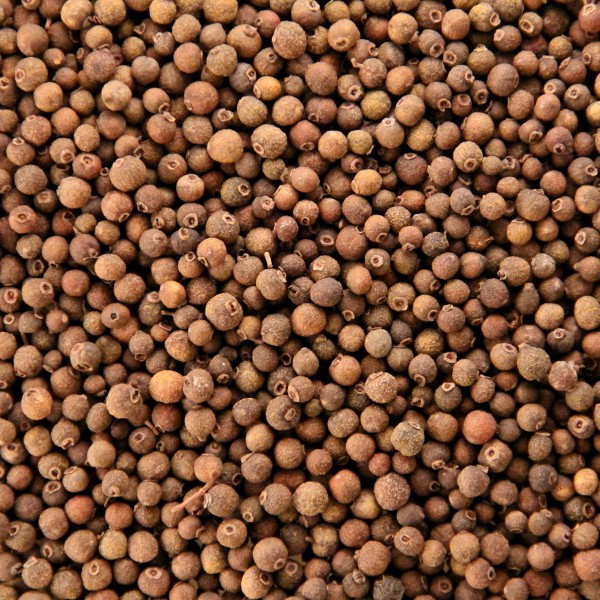
\includegraphics[width=0.3\linewidth]{imgs/spices/allspice-1.jpg}}
	\hfill
	\subfloat[\centering anise]{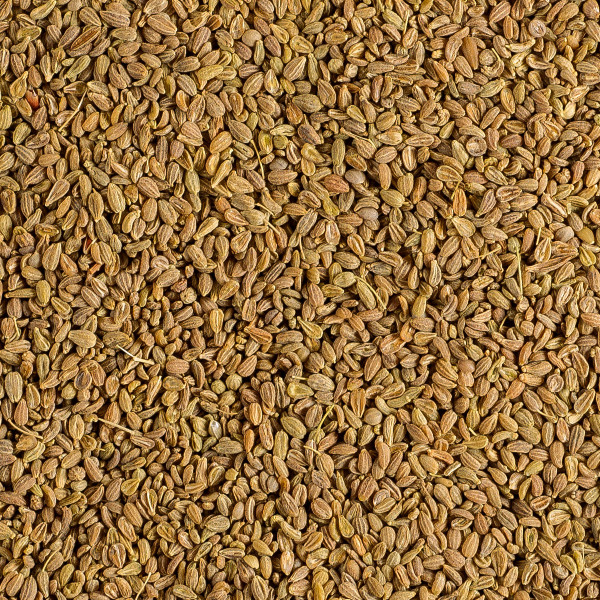
\includegraphics[width=0.3\linewidth]{imgs/spices/anise-1.jpg}}
	\hfill
	\subfloat[\centering asafoetida*]{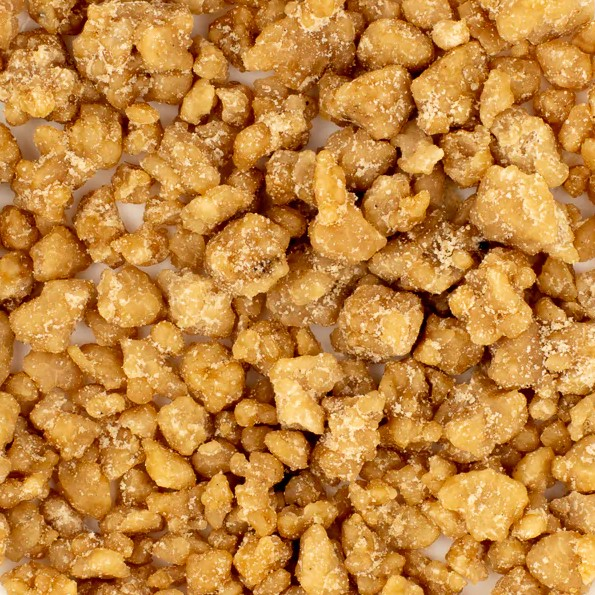
\includegraphics[width=0.3\linewidth]{imgs/spices/asafoetida-1.jpg}}
	\hfill
	\subfloat[\centering caraway]{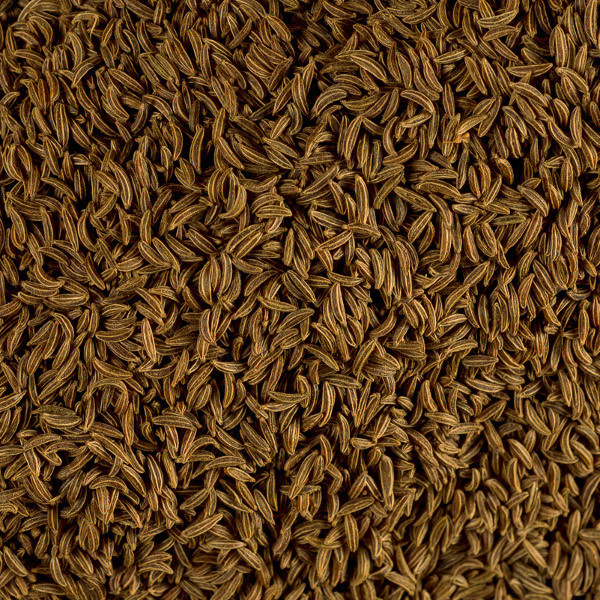
\includegraphics[width=0.3\linewidth]{imgs/spices/caraway-1.jpg}}
	\hfill
	\subfloat[\centering cardamom]{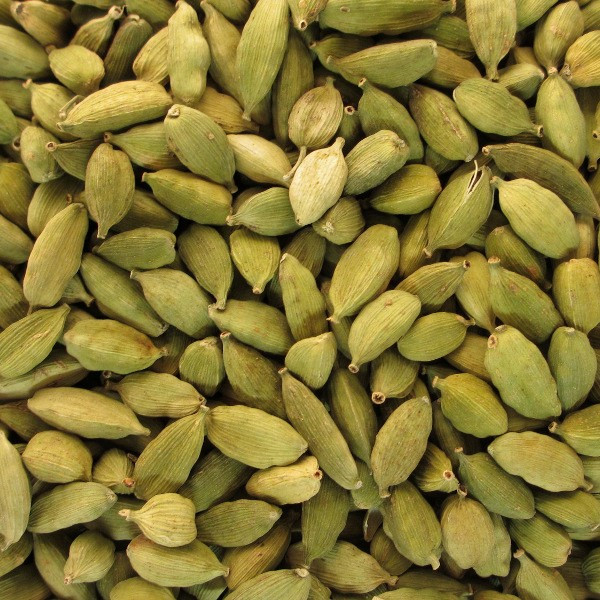
\includegraphics[width=0.3\linewidth]{imgs/spices/cardamom-1.jpg}}
	\hfill
	\subfloat[\centering cassia]{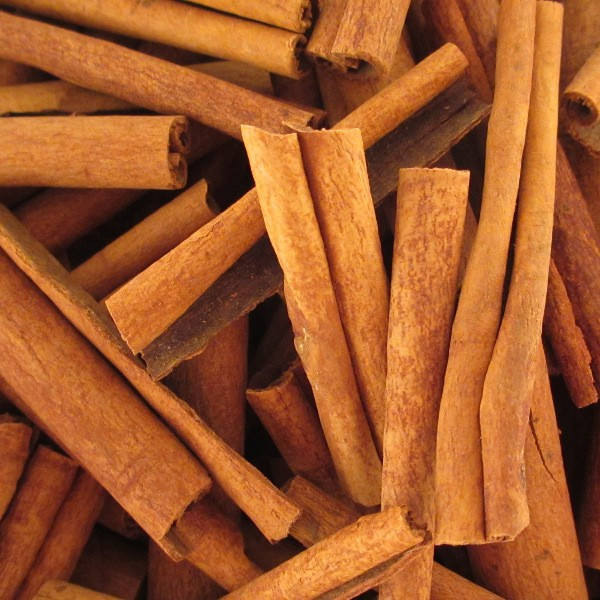
\includegraphics[width=0.3\linewidth]{imgs/spices/cassia-1.jpg}}
	\hfill
	\subfloat[\centering chile]{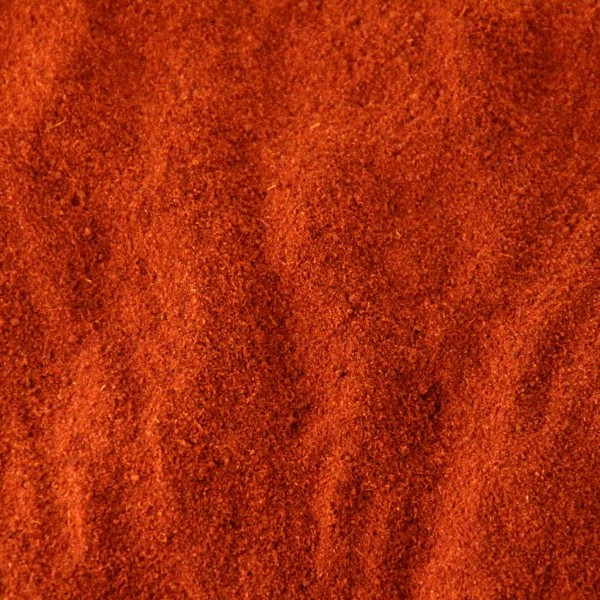
\includegraphics[width=0.3\linewidth]{imgs/spices/paprika-hungarian-1.jpg}}
	\hfill
	\subfloat[\centering cinnamon]{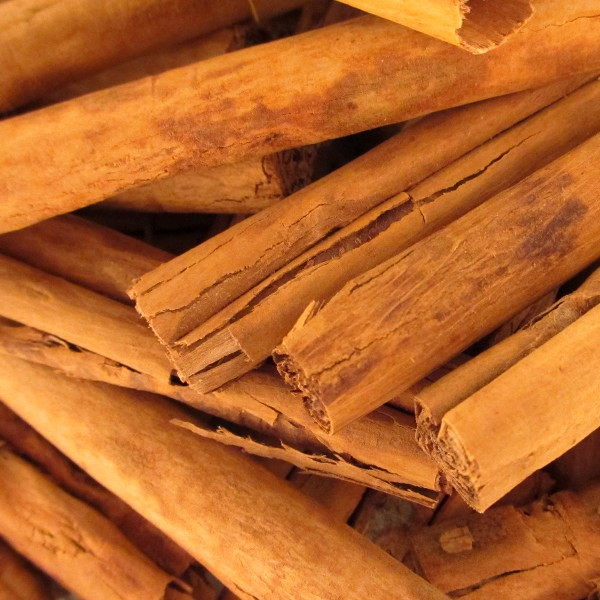
\includegraphics[width=0.3\linewidth]{imgs/spices/cinnamon-1.jpg}}
	\hfill
	\subfloat[\centering cloves]{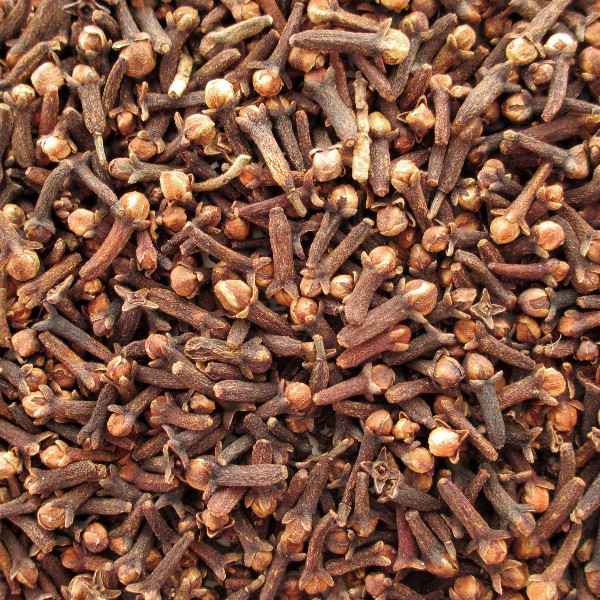
\includegraphics[width=0.3\linewidth]{imgs/spices/cloves-2.jpg}}
	\hfill
	\subfloat[\centering coriander]{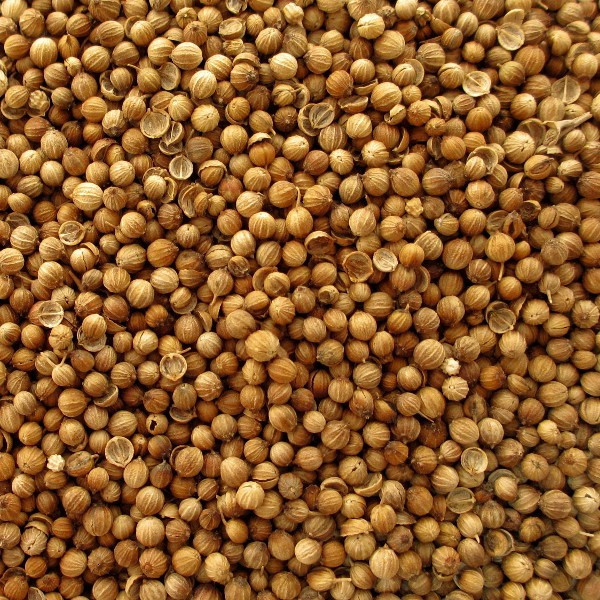
\includegraphics[width=0.3\linewidth]{imgs/spices/coriander-1.jpg}}
	\hfill
	\subfloat[\centering cumin]{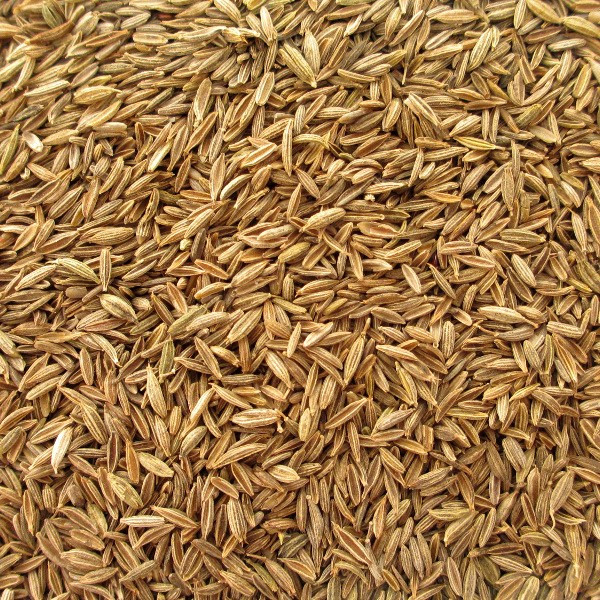
\includegraphics[width=0.3\linewidth]{imgs/spices/cumin-1.jpg}}
	\hfill
	\subfloat[\centering dill]{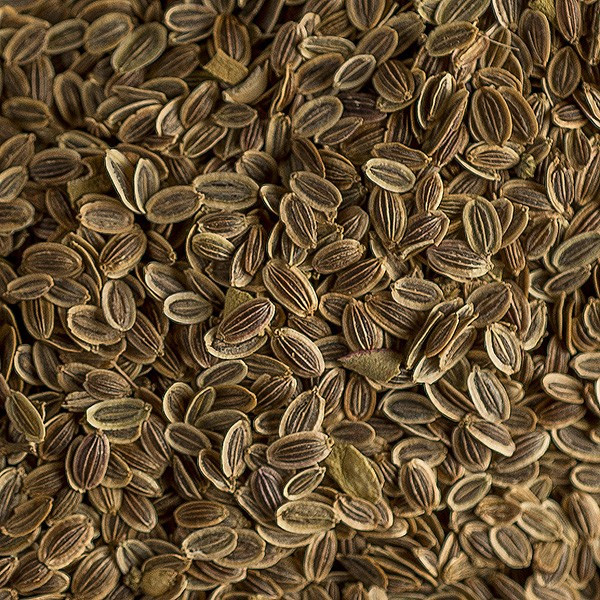
\includegraphics[width=0.3\linewidth]{imgs/spices/dill-1.jpg}}
	\caption[Photographs of the spices in this dissertation (I)]{Photographs of the spices in this dissertation (I). Credit: Aromatiques; *Glorian.}
	\label{fig:spice_imgs1}
\end{figure}

\begin{figure}[!ht]
	\centering
	\subfloat[\centering fennel]{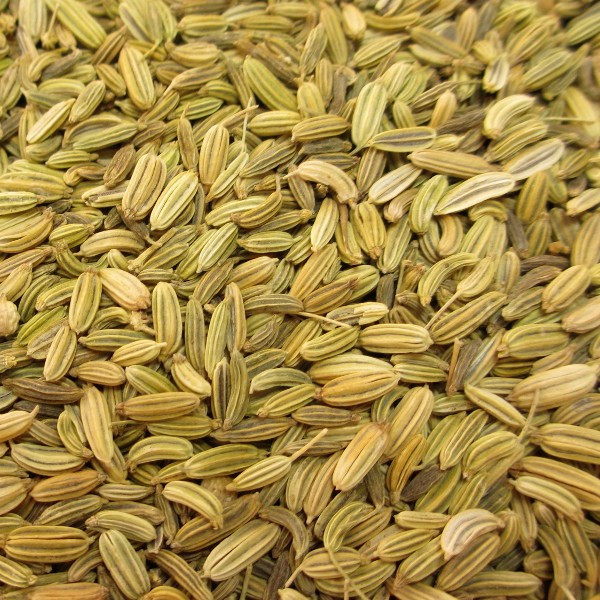
\includegraphics[width=0.3\linewidth]{imgs/spices/fennel-1.jpg}}
	\hfill
	\subfloat[\centering fenugreek]{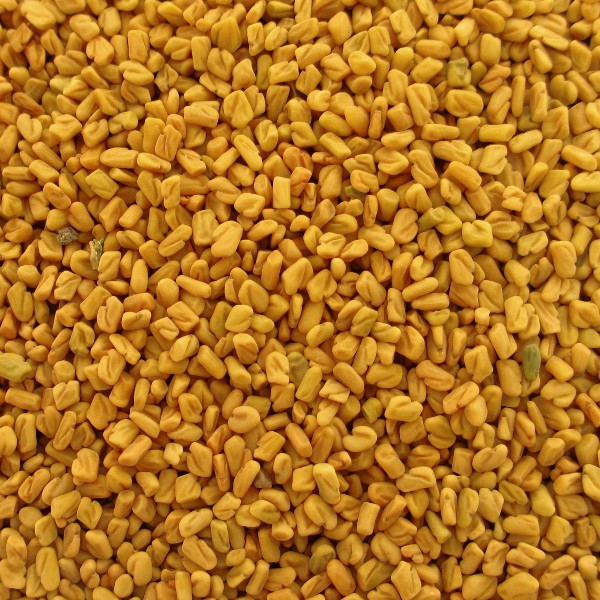
\includegraphics[width=0.3\linewidth]{imgs/spices/fenugreek-1.jpg}}
	\hfill
	\subfloat[\centering ginger]{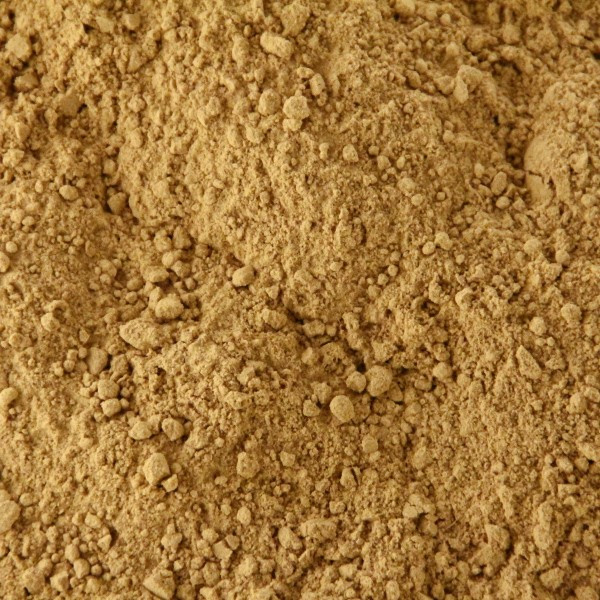
\includegraphics[width=0.3\linewidth]{imgs/spices/ginger-2.jpg}}
	\hfill
	\subfloat[\centering long pepper]{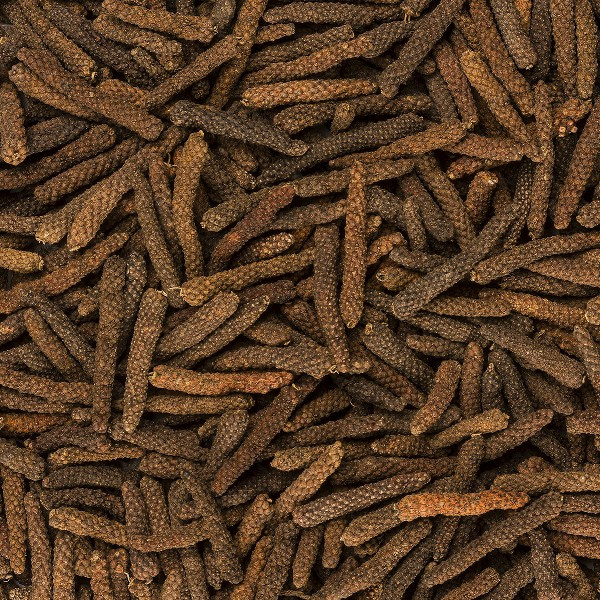
\includegraphics[width=0.3\linewidth]{imgs/spices/pepper-long-2.jpg}}
	\hfill
	\subfloat[\centering mace]{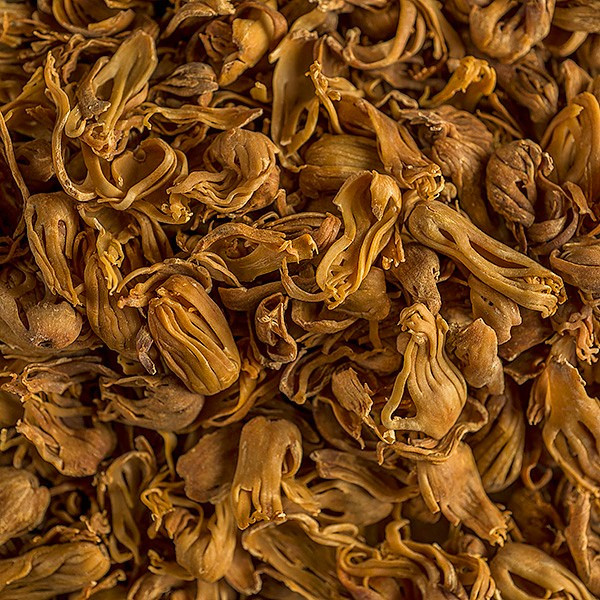
\includegraphics[width=0.3\linewidth]{imgs/spices/mace-2.jpg}}
	\hfill
	\subfloat[\centering nutmeg]{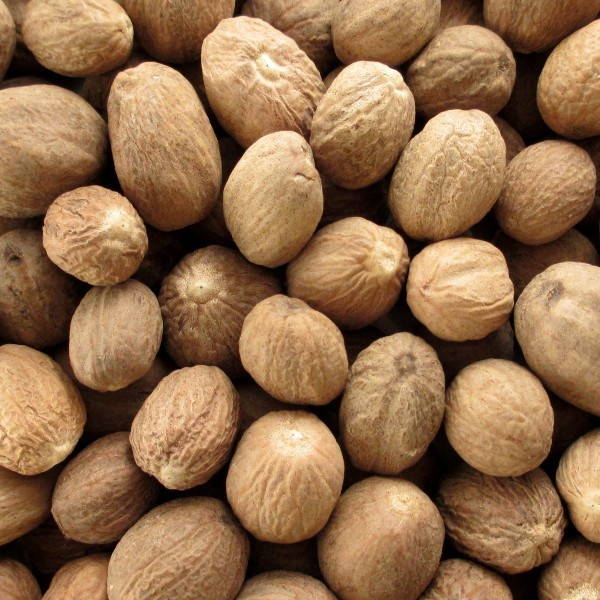
\includegraphics[width=0.3\linewidth]{imgs/spices/nutmeg-2.jpg}}
	\hfill
	\subfloat[\centering pepper]{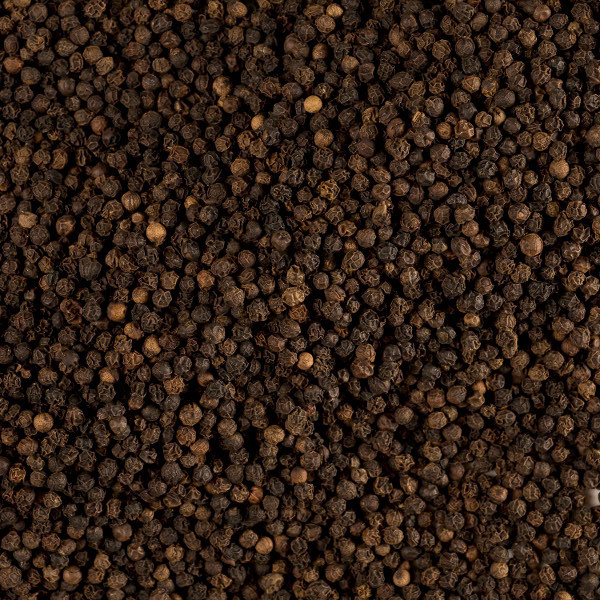
\includegraphics[width=0.3\linewidth]{imgs/spices/pepper-black-1.jpg}}
	\hfill
	\subfloat[\centering saffron]{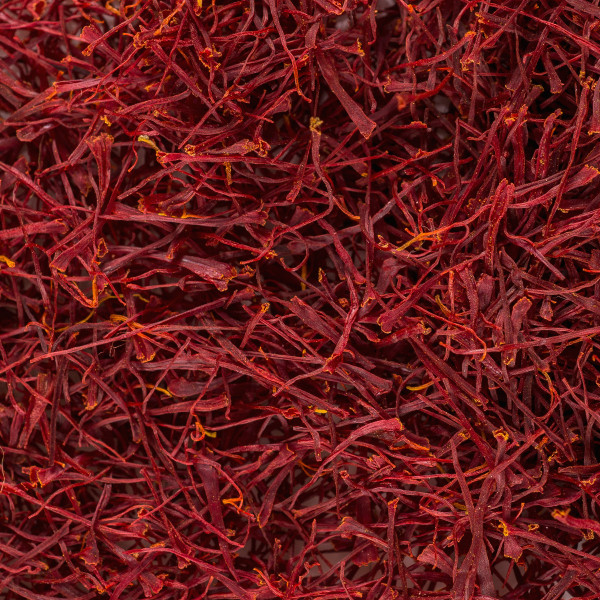
\includegraphics[width=0.3\linewidth]{imgs/spices/saffron-1.jpg}}
	\hfill
	\subfloat[\centering Sichuan pepper]{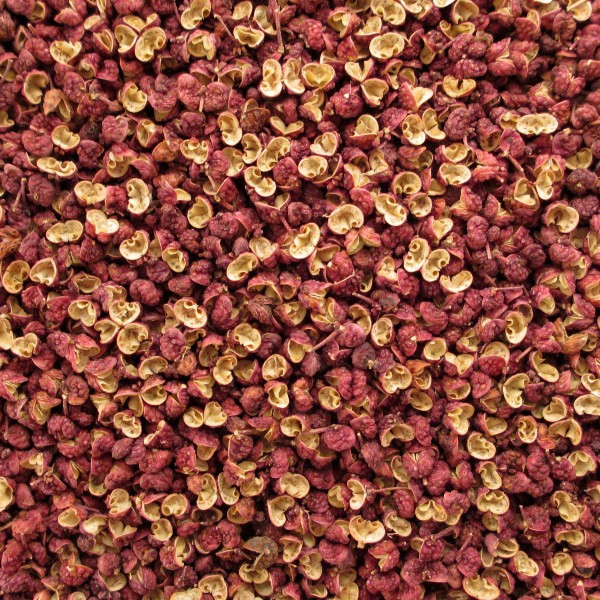
\includegraphics[width=0.3\linewidth]{imgs/spices/sichuan_pepper-2.jpg}}
	\hfill
	\subfloat[\centering star anise]{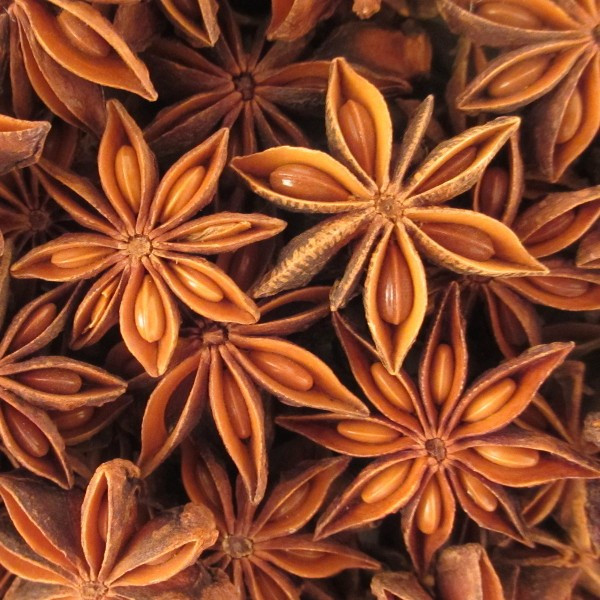
\includegraphics[width=0.3\linewidth]{imgs/spices/star_anise-1.jpg}}
	\hfill
	\subfloat[\centering turmeric]{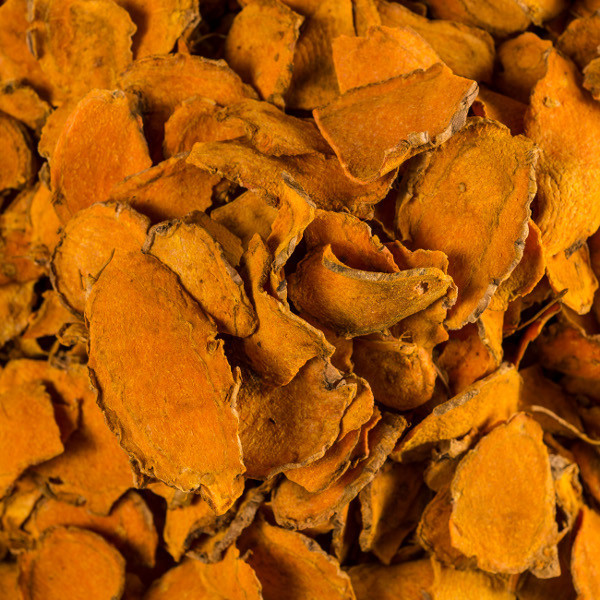
\includegraphics[width=0.3\linewidth]{imgs/spices/turmeric-1.jpg}}
	\hfill
	\subfloat[\centering vanilla]{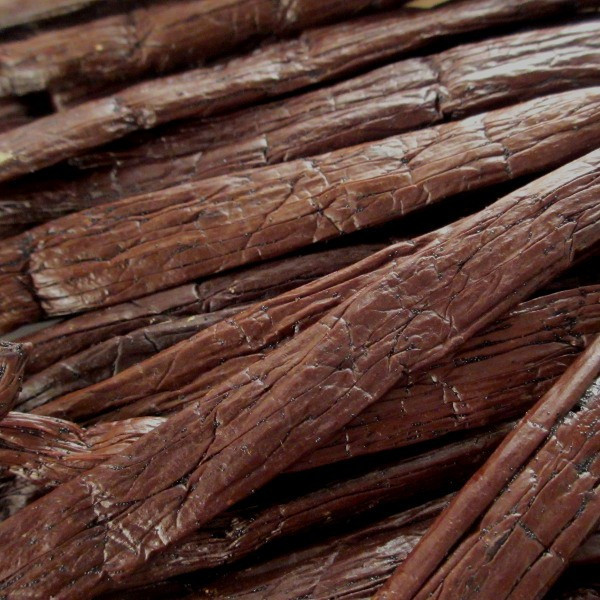
\includegraphics[width=0.3\linewidth]{imgs/spices/vanilla-1.jpg}}
	\caption[Photographs of the spices in this dissertation (II)]{Photographs of the spices in this dissertation (II). Credit: Aromatiques.}
	\label{fig:spice_imgs2}
\end{figure}

\clearpage % % Full page illustration
% \begin{figure}[!hbtp]
%     \centering
%     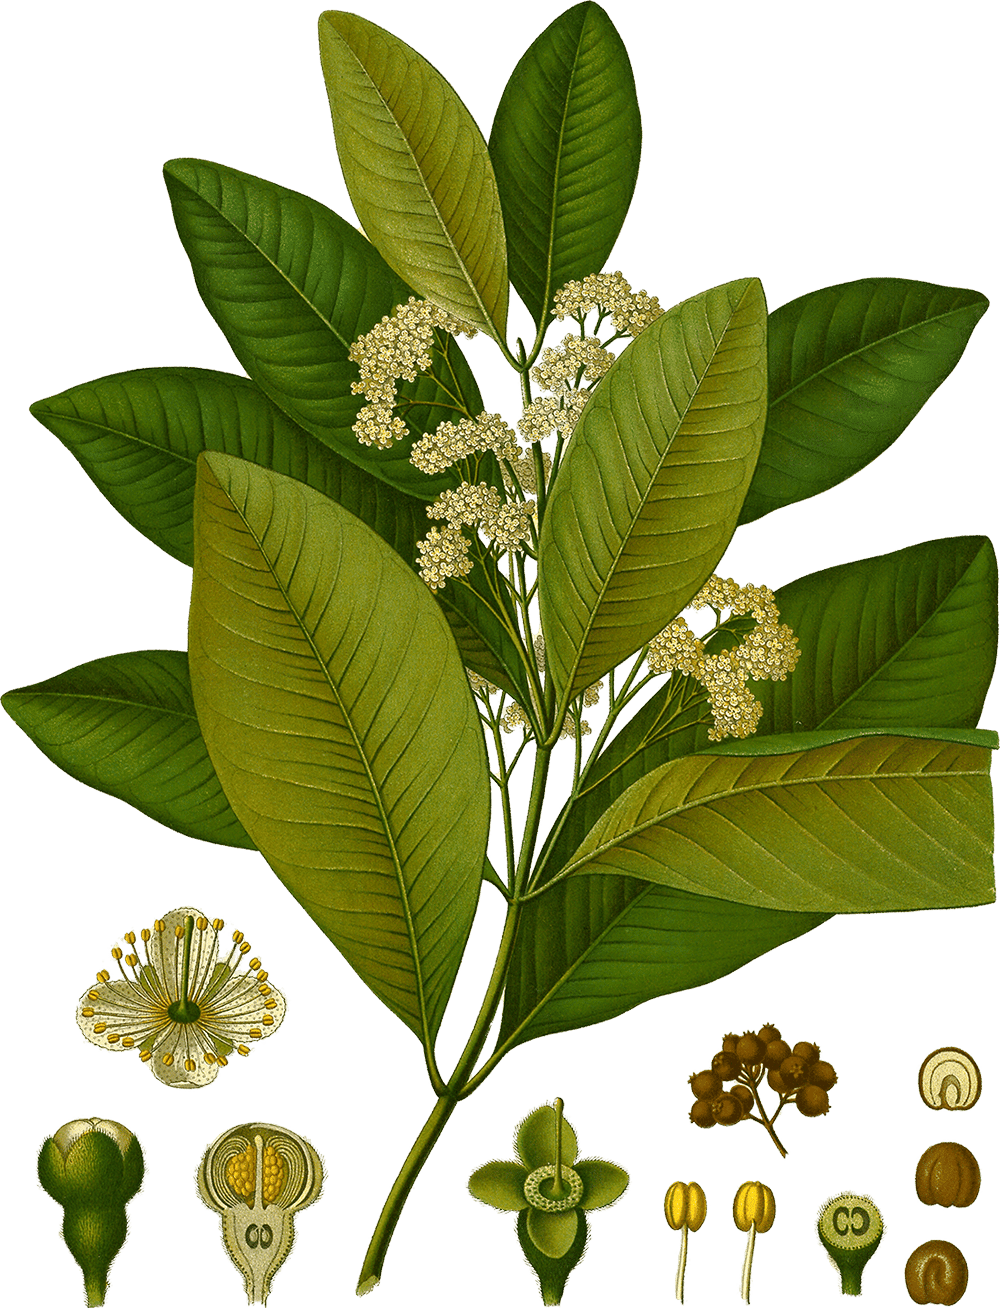
\includegraphics[width=\textwidth]{imgs/kohler/allspice_kohler_min.png}
%     \caption{\taxonn{Pimenta dioica}{(L.) Merr.} (syn. \taxonn{P. officinalis}{ Lindl.}), the allspice tree in Köhler's Medicinal Plants \pvolcite[]{2}[174]{kohler_kohlers_1887}.}
%     \label{fig:kohler_allspice}
% \end{figure}


% \begin{wrapfigure}{O}{0.5\textwidth}
%   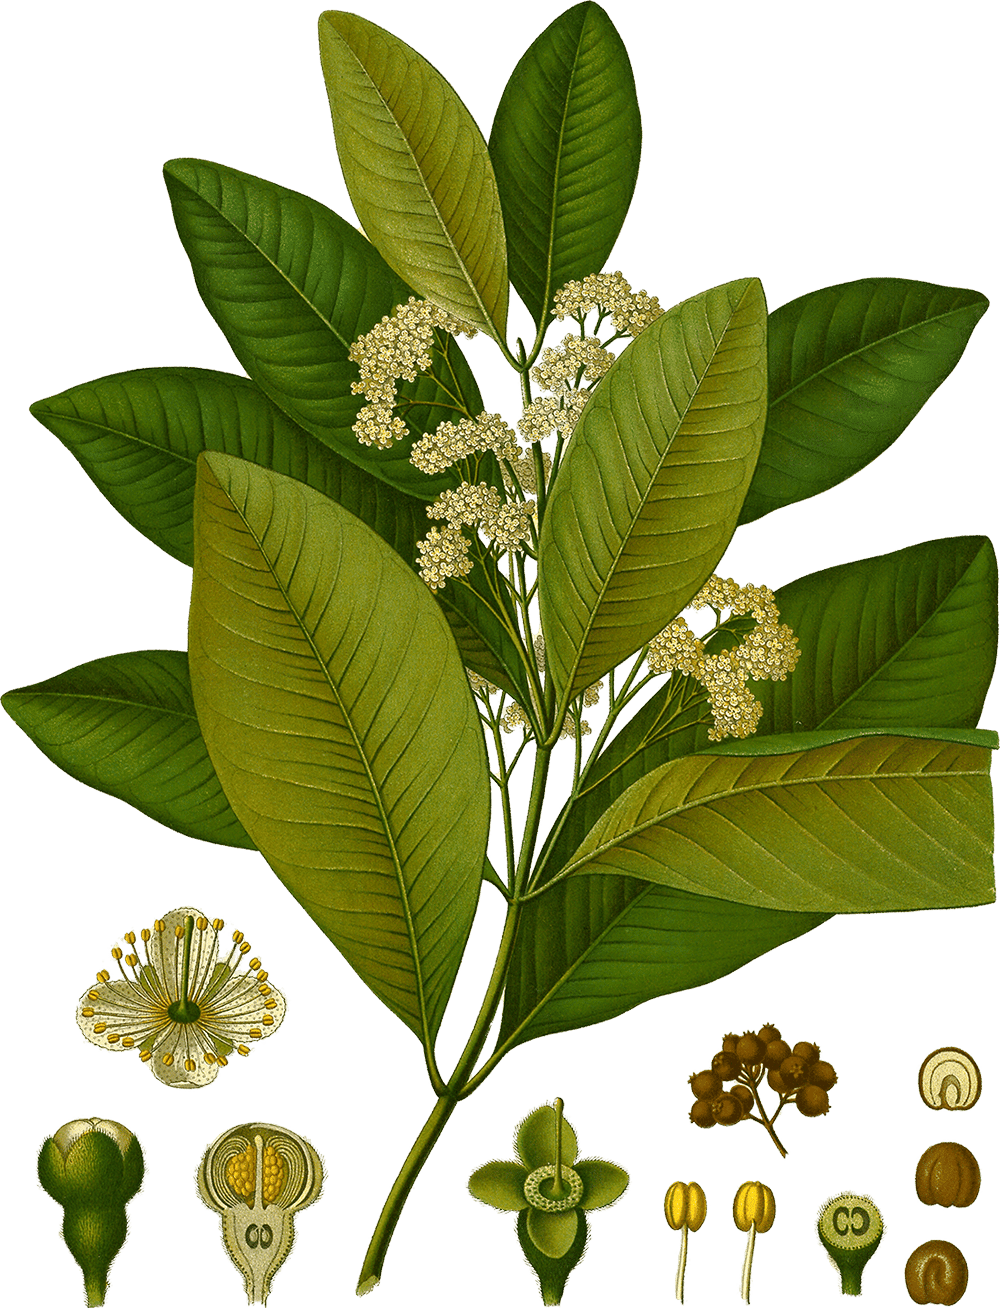
\includegraphics[width=0.5\textwidth]{imgs/kohler/allspice_kohler_min.png}
%   \caption{\textit{Pimenta dioica} {\small(L.) Merr.} syn. \textit{P. officinalis} {\small Lindl.} the allspice tree in Köhler's Medicinal Plants \pvolcite[]{2}[174]{kohler_kohlers_1887}.}
% \end{wrapfigure}


% \begin{wrapfigure}{o}{0.5\textwidth}
%     \includegraphics[width=0.5\textwidth]{imgs/spices/allspice.jpg}
%   \caption{Allspice berries}
% \end{wrapfigure}

\section{Allspice}
\label{sec:allspice}

\begin{spice}\label{spice:allspice}
\textsc{Allspice} \hfill \href{https://powo.science.kew.org/taxon/196799-2}{POWO} \\
\textbf{English:} \textit{allspice}; \textit{pimento; Jamaica pepper}. 
\textbf{Arabic:} {\arabicfont{فلفل إفرنجي}} \textit{fulful ifranjī} [Frankish pepper]. 
\textbf{Chinese:} {\tc{多香果}} \textit{duōxiāngguǒ} [many-spice-fruit]. 
\textbf{Hungarian:} \textit{szegfűbors} [clove-pepper]; \textit{jamaicaibors} [Jamaican-pepper]; \textit{amomummag} [amomum-seed].  \\
\noindent{\color{black}\rule[0.5ex]{\linewidth}{.5pt}}
\begin{tabular}{@{}p{0.25\linewidth}@{}p{0.75\linewidth}@{}}
Plant species: & \taxonn{Pimenta dioica}{(L.) Merr.} (syn. \taxonn{Pimenta officinalis}{Lindl.}) \\
Family: & \textit{Myrtaceae} \\
part used: & unripe fruit; leaf \\
Region of origin: & S. Mexico to C. America; Caribbean \\
Cultivated in: & Jamaica; Mexico; Honduras \\
Color: & dark brown \\
\end{tabular}
\end{spice}

\begin{figure}[!ht]
	\vspace{-4ex}
	\centering
	\subfloat[\centering berries]{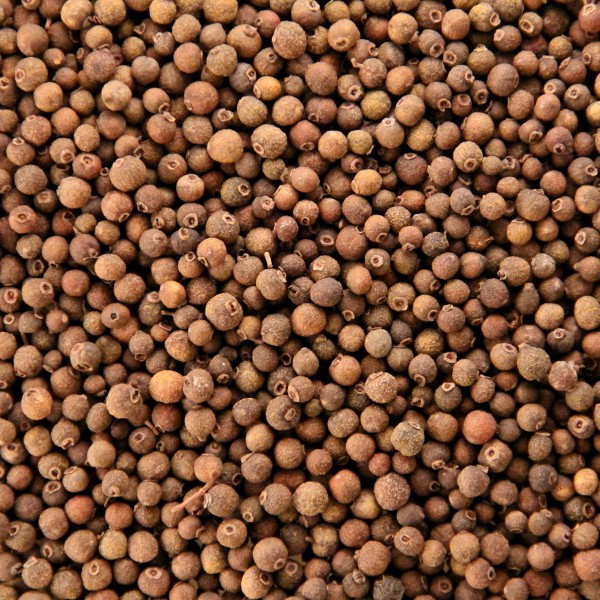
\includegraphics[width=0.3\linewidth]{imgs/spices/allspice-1.jpg}}
	\hfill
	\subfloat[\centering powder]{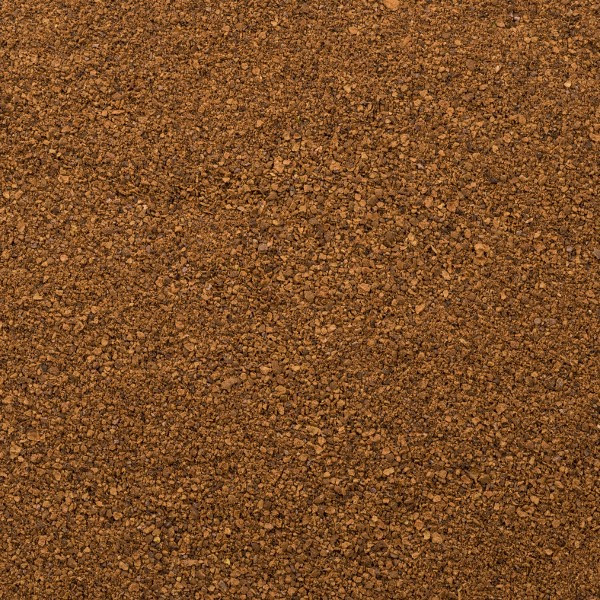
\includegraphics[width=0.3\linewidth]{imgs/spices/allspice-2.jpg}}
	\hfill
	\subfloat[\centering leaves]{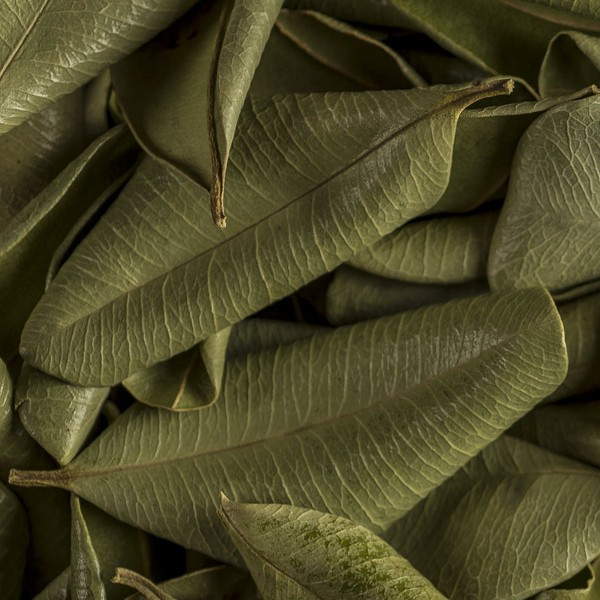
\includegraphics[width=0.3\linewidth]{imgs/spices/allspice-3.jpg}}
	\caption{Allspice berries, powder, and leaves from \textit{Pimenta dioica}.}
	\label{fig:allspice_imgs}
\end{figure}

\begin{note}
	Introducing the \textit{Spice profile box}. As it can be seen above in \textit{Spice profile} \ref{spice:allspice} presenting allspice, this business-card-like environment gives a quick reference of the spice under scrutiny in a concise way. This is intended to be a convenience for the reader to return and glance back at brief, factual information about a particular item whenever necessary. The box also contains a clickable link to the related plant species in a botanical database, \gls{POWO}, where more information can be found, such as the plants' biodiversity, distribution, botanical synonyms, as well as images of specimens.
\end{note}

%DESCRIPTION
Allspice, also known as pimento and Jamaica pepper, refers to the dried unripe fruits of a tropical evergreen tree growing in the Caribbean: the \textit{Pimenta dioica}. The dried berries are dark brown, hard to the touch, and 4--6 mm in diameter (thus larger than black pepper). Their signature crown is by a small ring of the calyx \autocite[210]{van_wyk_culinary_2014}. It is one of the few spices that do not come from the East; chili, vanilla, and allspice are the traditional three when one is listing spice products native to the Americas (disregarding cacao which is not considered a spice today). It is also the only spice that is exclusively cultivated on the western hemisphere \autocite[21]{duke_crc_2002}. The term \textit{allspice} is a coinage playing on the notion that the flavors and aroma of allspice is similar to that of clove, cinnamon, nutmeg, and black pepper \autocite[717]{mabberley_mabberleys_2017}---the most popular spices in Europe at the time when Europeans got in contact with this New World spice. People who only saw ground allspice but not whole, often tend to think that is in fact a spice mixture, after its name and rich flavor profile. Usually ground to powder, allspice is one of the key ingredients of Caribbean cuisine, especially jerk style dry-rub meat preparation. It is also used in European sausage making, pickling, baking, and flavoring liqueurs, it an overall ``handy spice''.\footnote{The Icelandic name is \textit{allrahanda}, literally `of all hands', meaning `for various purposes'; showing its multifaceted uses.} It also found its way into some Middle Eastern spice blends.


\begin{note}
\label{note:pimento}
Allspice is sometimes called pimento, which is also the name of a cultivar of \textit{Capsicum annuum}, famous from the Southern United States appetizer pimento-cheese. It is therefore important not to confuse allspice with the heart-shaped mild cherry peppers that North Americans also call pimiento or pimento. 
\end{note}

\subsection{The Botany, Origin, and  Cultivation of Allspice}

%PLANT
The allspice tree is a small mid-canopy tree or shrub with smooth, bay-like leaves and tiny white flowers. The berries turn dark purple if left to ripe, and the leaves and the bark are also aromatic \autocite[279]{riffle_tropical_1998}. Belonging to the myrtle family (\textit{Myrtaceae}), allspice is related to other aromatic trees, such as clove, eucalyptus, and the bay rum tree. Its binomial name is made up of \textit{pimenta}, the Portuguese (or corrupted Spanish) equivalent of `pepper', and \textit{dioica} `of two houses' (Greek \textit{di-} from \textit{dyo} `two' and \textit{oikos} `house'), indicating that the male and female flowers are found on different plants \pvolcite[]{2}[166]{peter_handbook_2012}.

%ORIGIN
Allspice is indigenous to the regions ranging from Southern Mexico to Central America and the Greater Antilles of the Caribbean, especially Jamaica \autocite[146]{czarra_spices_2009}. Where naturalized, it spreads by birds carrying the seeds. Allspice has been since introduced to a few neighboring places, such as Colombia, Venezuela, and Florida \autocite[][146]{powo_pimenta_2022}. In 1885 it was introduced from Jamaica to Hawaii and Kauai, 
% where it is designated as one of the most invasive horticultural plants of Hawaii \autocite{gisd_pimenta_2022}, 
and it even reached Tonga.

%CULTIVATION
Allspice is cultivated as a crop in a few countries, notably in Jamaica, Mexico, and to a lesser extent in Honduras and Grenada. The primary producer and the source of the highest quality being Jamaica. Saplings are grown from seeds, then soon transplanted when still small. The trees need well-drained soil and humid conditions \autocite[210]{van_wyk_culinary_2014}. It is one of the only spices that no one managed to grow in the East, transplantation efforts were quickly abandoned, and its commercial cultivation is confined to the Americas \autocite[21]{duke_crc_2002}. 
%HARVEST
Harvesting happens similarly to how black pepper is harvested; the still green, unripe fruits are picked by hand, and then dried under the sun.

%CHEMISTRY
The flavor of allspice mainly comes from the component eugenol, which is dominant both in the fruit and the leaves, but other compounds also add to the complexity of its aroma. Eugenol---also called clove oil, for it constitutes 80-90\% of the essential oil from clove buds \autocite[166]{barnes_herbal_2007}---is widely used as a flavoring agent by the food industry and in pharmacology, and is also found in cinnamon, nutmeg, and bay leaves. It has antiseptic, antibacterial, anesthetic, and analgesic properties \autocite{ulanowska_biological_2021}. The leaves of a related plant called the West Indian Bay Tree (\textit{Pimenta racemosa}) is used to produce bay rum, a popular essential oil used by the perfume industry for its spicy notes. 
% \todo{Contrary to popular belief, none of the above seems to be an ingredient in Old Spice\footnote{\url{https://www.fragrantica.com/perfume/Shulton-Company/Old-Spice-Original-14746.html}}}


% %USES
% \subsection{Culinary and Medicinal Uses}


% green 2006

% www.foodreference.com/html/fallspice.html
% The fruit and leaf oil are also used in men's toiletries - any time you see the word 'spice' in the name, such as in 'Old Spice' you can be sure that the fragrance comes at least in part from allspice oil. ??? no proof
% Pimento (Allspice) wood is used in Jamaica to cooked 'jerked' meats.

% Wyk:
% Allspice has become popular in some Western and East European countries, initially as a spice to replace cardamom. It is used to flavor a wide range of dishes, including meat stews, sausages, salted beef, pork, meat pastries, pickles, sauces and stuffings. Allspice is an essential ingredient of Caribbean cuisine (e.g.,jerk seasoning). It is used in Scandinavian smorgasbord, as well as fish, cheese and vegetable dishes. Mexicans use it in moles. Allspice is popular in Great Britain, where it is used in stews, sauces, confectionery, puddings and the traditional Christmas cake. Jamaican pimento dram and French liqueurs such as Benedictine and chartreuse are flavored with allspice.2 The spice, fruit oil or oleoresin extracts are commonly used in food processing, especially to flavor charcuterie items such as sausages, ham, salami and canned meats, as well as curry powders, condiments, relishes, ketchup, pickling spices and gravy mixtures. Leaf oil is used in ice creams, puddings, confectionery and liqueurs. 

% Czarra 146:
% Allspice is primarily used in the food industry in pickles, sausages, ketchup and canning meat. It can be also used as a spiced tea mix, in soups and curries and as a pickling spice.

% The fresh leaves of the allspice tree are used similarly to bay leaves in cooking, but they cannot be stored dry as opposed to the bay leaf; they lose their aroma.

%Where the tree is native, the wood is used to smoke meat.

% Duke 245
% Other Uses (Allspice) — Allspice of commerce is the dried unripe fruit, used as a condiment; in baked goods, chutney, ice cream, ketchup, mixed spices, pickles, sauces, soups; and in flavoring sausages and curing meats. Allspice powder consists of whole ground dried fruit. It’s called “allspice” because it supposedly embraces the aromas of cinnamon, cloves, and nutmeg. To make an allspice substitute, merely combine one part nutmeg, two parts cinnamon, and two parts clove (RIN). Mexican Indians used allspice to flavor chocolate. I use it to flavor eggnog. Allspice is an essential ingredient of the rubs and marinades used in seasoning Jamaican jerked foods, which are also flavored by the smoke of pimento wood fires (FAC). In Jamaica, a local drink called “pimento dram” is made of ripe fruits and rum. It is regarded as a panacea. Allspice is used in such liqueurs as Benedictine and Chartreuse. A volatile oil, extracted from the spice and leaves, is used to flavor essences and perfumes and as a source of eugenol and vanillin. The oil is also used in flavoring beverages, candies, chewing gums, liqueurs, meats and sauces, and in Asian perfumery and shaving lotions. Bahamians make a pleasing tea from the leaves. Costa Ricans use the leaves as a spice. Many ethnic groups use the leaves in tea. Saplings are used as walking sticks and umbrella handles (DAD, FAD).

% Wiki:
% Allspice is also one of the mainly used spices in Polish cuisine (used in most dishes, soups and stews) and is commonly known under the name English herb (Polish: ziele angielskie). 
% At the time allspice was encountered by Christopher Columbus during his second voyage to the New World, it was found only on the island of Jamaica, where the plant was readily spread by birds. Allspice was introduced into European and Mediterranean cuisines in the 16th century. To protect the pimenta trade, Jamaican growers guarded against export of the plant. Many attempts at growing the pimenta from seeds were reported, but all failed. Eventually, passage through the avian digestive tract, whether due to the acidity or the elevated temperature, was found to be essential for germinating the seeds,[7] and successful germination elsewhere was enabled. Today, pimenta grows in Tonga and Hawaii, where it has become naturalized on Kauaʻi and Maui.[8] It continued to be grown primarily in Jamaica, though a few other Central American countries produced allspice in comparatively small quantities.[9]

% Duke 21?

% the allspice fruits were used to preserve meats on long voyages. These preservative activities are due to some of the aromatic and antiseptic compounds which abound in allspice (anethole, caryophyllene, eugenol, linalool, pinene, and terpinene).

\subsection{The History of Allspice}

% https://journals.openedition.org/ethnoecologie/6261

There is not much we know about allspice before the arrival of the Europeans, except that the Aztecs used it to spice up their chocolate drink \autocites[27]{farrell_spices_1985}, although \textcite[145, 177]{dalby_dangerous_2000} doubts this was the case that early on. According to \textcite[21]{duke_crc_2002}, the Maya used allspice for embalming. We know that it reached Europe as a consequence of Christopher Columbus's voyages. Spanish colonizers must have encountered allspice in the West Indies sometime after Columbus and his crew explored the islands of Hispaniola, Cuba, and Jamaica, and the year 1494 is reported \autocite[12]{opara_culinary_2021}. Columbus himself did not find it. In fact, he did not recognize any spice he was so keen on finding---pepper, cloves, nutmeg, cinnamon---but kept himself and his patrons in the delusion that he will. In his first letter to Ferdinand and Isabella he writes: ``On this island there are many spices and great mines of gold and other metals. [...] I believe that I have found rhubarb and cinnamon.'' \autocite[10-18]{columbus_spanish_1893} ---in reality, he had none.\footnote{Columbus's first letter of his first voyage, sent on March 4, 1493 from Lisbon to the Spanish court (and its translation) is also available online at King's College London. Transcription: \url{http://www.ems.kcl.ac.uk/content/etext/e021.html}, translation: \url{http://www.ems.kcl.ac.uk/content/etext/e022.html}}

He was adamant that the islands he \textit{discovered} were full of spices and brought up excuse after excuse (out of season, etc.) after every voyage he returned with no spice \autocite[149]{dalby_dangerous_2000}. He also believed that he was in India or Cathay, on one of the outlying islands. Between apologies, Columbus also promised more gold, silver, cotton, mastic, and slaves. As \textcite[150]{dalby_dangerous_2000} reports, what he recorded in his private journal is a bit more honest and realistic version of events: ``I think that many trees and plants grow here which will be highly valued in Spain for dyes and medicinal spices. But I am sorry to say that I do not recognize them.'' Columbus repeatedly regrets his ignorance in botany in his journal \autocite[see also][57]{columbus_journal_2010}.

Interestingly, authors love to claim that Columbus brought back allspice (together with vanilla and chili): ``He returned with allspice from the West Indies, chilies from Mexico and vanilla from Central America.'' \autocite[17]{craze_spice_1997}, and ``Columbus brought it back to Europe thinking it was pepper.'' \autocite[146]{czarra_spices_2009}, or ``Though he did not find the Spice Islands, Columbus brought allspice, vanilla and red peppers from the West Indies back to his Spanish supporters.'' \autocite[1]{parthasarathy_chemistry_2008}. This is not true, he most likely never even saw allspice, but it was reported him that it is there and can be cultivated, along with cinnamon, and mulberry for silk production \autocites[151]{colon_life_1959}. Columbus returned from his first voyage of 1492--93 with some gold nuggets and jewelry, pearls, a hammock, tobacco, the turkey, and a few poor captured Taínos, but no spices were presented to the Spanish monarchs Ferdinand and Isabella. He did bring back pineapple and cassava \autocite[11]{turner_spice_2004}. 

Diego Álvarez Chanca, the court appointed physician who accompanied Columbus on his second expedition in 1493 is often credited with bringing home both chili, and allspice \autocites[]{mccormick_history_nodate}, but in his 1494 letter describing the flora and fauna, he only mentions \textit{agi}, also \textit{axi}---modern Spanish \textit{ají} from Taíno---\autocite[see][34]{corominas_breve_1987}, and that the natives use it to season their food, with what we now know as \textit{Capsicum annuum}: the chili pepper \autocite[311]{chanca_american_2003}.

In the following century the Spanish tried to turn Mexico into a spice plantation by transplanting eastern spices, an effort that mostly failed. Only after this did the colonizers start to pay proper attention to native spices \autocite[6]{machuca_past_2020}. 

Francisco Hernández de Toledo, King Philip II's court physician and naturalist spent 7 years in New Spain between 1571--1577, studying its species and conducting interviews with the natives. He was the first to formally describe allspice. He called it \textit{Pipere Tavasci} `Tabasco pepper' (today \textit{Pimienta de Tabasco}, after the region of Tabasco, famous today for a brand of hot sauce. Hernández also recorded the Nahuatl name of allspice: \textit{xocoxochitl} `sour flower'.\footcite[cf.][xococ; xochitl]{ond} Hernández likens the flowers to pomegranates, and and the aroma to that of orange blossoms, describing it to be very pleasant and attractive, with a sharp taste of the fruit. \autocite[2]{hernandez_cuatro_1615}. In \textcite{machuca_past_2020}'s translation:

\begin{quote}
    ``Xocoxochitl meaning sour flower, is a large tree, with leaves like those of the oranges, red flowers like a pomegranate, but with an aroma like the orange blossom, and in such a smooth and pleasant way, that even the leaves of the tree add to its attraction: the fruit is round, and hangs in clusters, which at first appear green, and then beige, and finally towards black: it is sharp and scathing to taste, and good-smelling'' 
\end{quote}

According to \textcite{machuca_past_2020}, although allspice was known by the Spanish from early on ``there are few historical records of its production and trade'', and only in the \nth{18} century started they to consider American products to have economic potential.
 
Allspice berries are around 30\% larger then peppercorns, and since their color and shape resembles black pepper, and it gave a spicy taste to food, it is no wonder that the Spanish called them \textit{pimiento} `pepper'. The Portuguese version is \textit{pimento}, and later the botanical name \textit{Pimenta} was given to the genus of plants related to allspice \autocite[26]{farrell_spices_1985}. I disagree with the often repeated trope that the Spanish explorers mistook allspice berries for pepper and called them \textit{pimiento} ``by mistake''\footcite[allspice \link{https://www.britannica.com/plant/allspice}]{britannica_spice_2022}, these people knew exactly what they were looking for, and that what they have found is not the mighty black pepper; but for them it was a kind of pepper. The crew showed samples of pepper and cinnamon to presumably confused Native Americans hoping for directions, and as Columbus wrote in his journal on the \nth{4} of November, 1492, they indicated by sign language that there is a lot of it around \autocites[21]{duke_crc_2002}[67]{columbus_journal_2010}. The Europeans, however, soon recognized the value of allspice, even if it was not the expensive black pepper, but still more pungent and exotic than some cheap Old World substitutes, the juniper and myrtle berries (which are very similar to allspice in appearance and usage)  \autocite[150]{dalby_dangerous_2000}.

In short, allspice was introduced to Europe by the Spaniards in the \nth{16} century, its import was first recorded in 1601, according to \textcite{britannica_allspice_nodate} and \textcite[26]{farrell_spices_1985}. After 1655, when Jamaica became a British colony for nearly three centuries, the Brits developed a taste for allspice and started to use it to season meat dishes, sauces, and pickles \autocite[74]{green_field_2006}. They were also responsible for its spread to some extent which is illustrated by the names of allspice in some languages, e.g.,Polish \textit{ziele angielskie} `English herb'.

% Allspice was first exported to Europe in 1601 as a substitute for cardamom. ?? Farrell 26

% https://www.mexconnect.com/articles/3799-fragrant-flavorful-allspice-an-essential-mexican-seasoning/

% peter 2 167
% The berries reached London in 1601 as described by Clusius in his Liber Exoticorum and the plants were first cultivated in England in a hot house in 1732 (Weiss, 2002). Before World War II, allspice was more widely used than today; however, during the war many trees were cut down and there was a shortage of the spice. Although cultivation was taken up after the war, production never fully recovered.


\subsection{The Names of Allspice}

Allspice is a fascinating case, because it gives us examples for a plethora of names that showcase us many of the motivations, mechanisms, and solutions people choose when naming spices. As I mentioned before, some people are puzzled if allspice is a spice blend or not. The names in some languages often just add to the confusion, for example French \textit{quatre-épices} (lit. `four spices') can have the sense `allspice', but also `a kind of spice mix' made up of four different spices.\footcite[quatre-épices \link{https://www.cnrtl.fr/definition/quatre-\%C3\%A9pices}]{tlfi}


% All these names can be explained by the characteristics, use, and journey of allspice. Let us now consider the names in English, Arabic, and Chinese.

\subsubsection{English}

\begin{etymology}\label{ety:allspice}
\textbf{English} \textit{allspice}, from \textit{all} + \textit{spice}; after the flavor profile that resembles the combined aroma of cloves, nutmeg, cinnamon, and black pepper, 1621\footnote{\textcite[s.v. allspice]{oed}}
\end{etymology}

\begin{note}
	Introducing the \textit{Etymology box}. This environment, as seen above in \textit{Etymology} \ref{ety:allspice}, offers a quick look at a words' origins and development.
\end{note}

Since its introduction to the spice cabinet, allspice has been known by many names from which currently \textit{allspice} \index{allspice|textbf} seems to be prevailing. \textit{Allspice} was formed by compounding \textit{all} and \textit{spice}, for its flavor was perceived to be a combination of four characteristic spices that the Europeans knew and sought after: black pepper, cinnamon, cloves, and nutmeg.\footcites[allspice]{oed}[]{britannica_allspice_nodate} It was first recorded in 1621: ``Ambergreese, nutmegs, and all spice.''\footcite[allspice]{oed}, and probably inspired the French \textit{toute-épice} `all-spice', attested in 1762.\footcite[toute-épice \link{https://www.cnrtl.fr/etymologie/toute-\%C3\%A9pice}]{tlfi}

Sadly, the original word for allspice was lost with the demise of the native Taíno people of the Caribbean, nevertheless we got Taíno\footnote{Taíno is a now extinct Arawakan language.} words such as barbecue, \textit{cassava}, \textit{guava}, \textit{hammock}, and \textit{tobacco} \autocite[229]{rafinesque_american_1836}. As we concluded before, it is assumed that it was the Spanish who first got in contact with the allspice berry, and that they simply called it \textit{pimienta} `pepper'.

\begin{etymology}\label{ety:pimento}
\textbf{English} \textit{pimento} `allspice; sweet pepper', ca. 1660
< partly \textbf{Portuguese} \textit{pimenta} `allspice; sweet pepper; black pepper'
< and partly \textbf{Spanish} \textit{pimiento} `hot and sweet pepper; formerly also black pepper; pepper plant of both kinds', earlier \textit{pimienta} `black pepper; peppercorn; ground pepper' \nth{13} c., 1495
< \textbf{Medieval Latin} \textit{pigmenta} `plant juice; food seasoning; condiment; spices; perfumes', plural of \textit{pigmentum}
< \textbf{Latin} \textit{pigmentum} `colour, paint; ointment; drug; spiced wine', from \textit{pingō} `to paint' + \textit{-mentum} `instrument'\footnote{\textcite[s.v. pimento]{oed}; \textcite[s.v. pimento]{oed}; \textcite[s.v. pimiento]{oed}; \textcites[415]{gomez_de_silva_elseviers_1985}[495]{corominas_breve_1987}; \textcite[s.v. pigmentum]{lewis_latin_1879}}
\end{etymology}

For a long time \textit{pimento} (and to a much lesser extent \textit{pimiento})---the words for `pepper' in Portuguese and Spanish, respectively---was commonly used in English to refer to allspice. This is still the case in Jamaican English for example, where the term \textit{allspice} is not used. In North American English however, \textit{pimento} now rather refers to a small, round variety of chili pepper (\textit{Capsicum annuum}), commonly known as cherry pepper explained in \cref{note:pimento}. 

The corruption and mix-up between the English words \textit{pimento} and \textit{pimiento} and their origins is as confusing as it gets. For the sake of a clear understanding, let us first consider the modern names for allspice in Spanish: \textit{pimienta de Jamaica}, and Portuguese: \textit{pimenta-da-jamaica}. In both cases, \textit{pim\-(i)enta}, with a final \textit{-a}, means `pepper', referring to peppercorns of the usual black and white pepper (\textit{Piper nigrum}). In Spanish and Portuguese, the words endings of \textit{-o} and \textit{-a} mark the grammatical gender, the significance of which dissipates in English. It is important to remember however, that the Spanish form \textit{pimienta} emerged first from a Latin neuter plural suffix in the \nth{13} century. Thus, perhaps a century or so later when the word \textit{pimienta} was already embedded in Spanish, speakers perceived the word as a feminine noun, and a vacuum of a masculine counterpart emerged. This allowed for a practical differentiation by gender between the peppers of the Old Word and the New World. \textcite[459]{corominas_breve_1987} explains that \textit{pimiento} derived from \textit{pimienta}, and it was first applied in the Americas for the red fruits of the chili.

\textcite[415]{gomez_de_silva_elseviers_1985} makes the most compact distinction: ``\textit{pimienta} `(black) pepper; allspice', \textit{pimiento} `(hot and sweet) pepper' ''. In contemporary Spanish, \textit{pimiento} (the masculine form) refers to the fruits and plants of the \textit{Capsicum} family, e.g.,the numerous spicy chilies and mild bell peppers of red, green, and yellow, while \textit{pimienta} (the feminine form) refers to the small round fruits of black and white pepper and its powdered forms. The distinction seems consistent, belonging to this latter group see for example \textit{pimienta dulce} `sweet pepper', and \textit{pimienta gorda} `fat pepper' both of which refers to allspice, not to be confused with \textit{pimiento dulce}, which refers to sweet paprika powder.\footcite[pimiento, -a]{dle}

\textit{Pimento} in English is a partly Portuguese, partly Spanish borrowing, while \textit{pimiento} comes from Spanish. In fact, it is explained in the \gls{OED} that in the `allspice' sense of the word, \textit{pimento}, from Portuguese \textit{pimenta (da Jamaica)}, went through an alteration influenced by the Spanish word form, which is not attested in the `allspice' sense. Ergo, Spanish \textit{pimiento} maybe did not refer to allspice in Spanish at the time when the borrowing happened. And if so, \textit{pimento} is a borrowing from Portuguese \textit{pimenta} meaning `pepper' and, as \textit{pimenta da Jamaica}, `allspice', influenced by Spanish \textit{pimiento} `chili, sweet pepper', also in the sense of the pepper plants of both kinds (chili and black). Spanish \textit{pimiento} formerly had the sense of `black pepper, peppercorns, and ground pepper' (before 1495), with an earlier form \textit{pimienta} (\nth{13} century), now usually in sense ground pepper and peppercorns\footcite[pimento]{oed}. The Portuguese connection is only discussed by the \gls{OED}, other dictionaries do not mention it. A direct Spanish borrowing is also plausible if we consider that it was the Spanish who most likely brought it back first, they probably called it \textit{pimiento/-a}, and they were responsible for its subsequent diffusion in Europe. English spellings varied greatly of this this Romance word, using forms such as \textit{piemente} in the late 1600s. 

The origin of these words is the classical Latin \textit{pigmentum} `a material for coloring, a color, paint, pigment', with a transferred meaning `the juice of plants' in post-classical Latin.\footcite[pigmentum \link{http://www.perseus.tufts.edu/hopper/morph?l=pigmentum\&la=la\&can=pigmentum0\#lexicon}]{lewis_latin_1879} The word \textit{pigmentum} is made up of \textit{pingō} `to paint' and \textit{-mentum}, a suffix denoting an `instrument, medium', well recognizable from Romance languages and English (i.e.,excite\textit{ment}).
According to \textcite[459]{corominas_breve_1987}, Catalan \textit{pimienta} is attested in the \nth{13} century and it comes from the plural (\textit{pigmenta}) of Latin \textit{pigmentum} `coloring, paint', which already meant `drug, ingredient', and later, `condiment' in Medieval Latin. Derived from this, in 1495 \textit{pimiento} was applied to the plants bearing the pungent red fruits of the Americas. \textit{Pigmentum} also entered English as \textit{pigment} `paint, dye, ingredient in an ointment, drug'. According to the \gls{OED}, Medieval Latin \textit{pigmentum} also referred to spiced drinks (\nth{9} century), perfumes, and hence spice in general. Old French cognates support this, \textit{pigment} had the sense of `balm, fragrant spice' in the \nth{12} century, Anglo-Norman \textit{pigment/piment} meant `spice, spice wine'\footcite[pigment]{oed}, and Middle English \textit{pihmentum} (\nth{12} century, later \textit{piment}) had a sense of ``a spiced drink, a remedy or concoction containing spices'',\footcite[pigment]{oe} ``a sweetened, spiced wine used for refreshment and in medical recipes; a medicinal potion''.\footcite[piment]{med} \textit{Piment} in French were later applied for chili, especially the cultivar of cayenne pepper. (The \gls{OED} points to the sense `cayenne pepper' in a ``\nth{10} century French source'', which must be an error.)


Allspice is also known as \textit{Jamaica pepper}, for it mainly grows on the island and the historical reasons described above. Many languages calqued \textit{pimienta de Jamaica} from Spanish, or another transmitting language (e.g.,Italian \textit{pepe della Giamaica}). \textit{Jamaica pepper} was first recorded in 1661: ``A kind of Pepper, that tastes like Cloves, and very Aromatick (known by the name of Iamaica-Pepper)''.\footcite[Jamaica]{oed}

The name \textit{myrtle pepper} \index{pepper!myrtle} echoes the similarities of the allspice tree with European myrtle (\textit{Myrtus communis}), especially after the resemblance of their purple berries. Beyond the physical resemblance, myrtle berries are also edible, and are also dried to add to pepper mills as a spice. Furthermore, the European myrtle has aromatic leaves and wood as well, and it is used to grill and smoke meat in Southern Europe since Roman times, especially on Sardinia and Corsica; the same way the Caribbean people use allspice wood and leaves. The myrtle berry appears in Roman and Greek mythology as well \autocite[186]{van_wyk_culinary_2014}.

The name \textit{clove pepper} has ``chemical reasons'', namely that this name arises from the aroma of allspice that reminded people of clove. This is due to its eugenol content we discussed above. \textit{Szegfűbors} lit. `clove-pepper' is the most common name for allspice in Hungarian still, and it is used in sausage making.

One of the most interesting spice names we can come across in my opinion is \textit{newspice}. The term is now archaic in English, but the idea still exists in a few European languages, such as Serbian and Macedonian \cy{најгвирц} \textit{najgvirc} from German (\textit{Neugewürz}), Czech and Slovak (\textit{nové koření/korenie}), and Turkish \textit{yenibahar} and Romanian \textit{ienibahar} from Ottoman Turkish \ar{یڭیبهار} \textit{yeñibahar}; all the above literally meaning `new spice'.

The reason behind these names is that during the 17-\nth{18} centuries, allspice ``suddenly'' arrived to Central and Eastern Europe as a new (and possible marketed as a trendy) spice. This happened a century after the red hot paprika took the world by storm (by \nth{16} century it reached Hungary from the Ottoman Empire), and while the chili did not conquer northern Europe, allspice---to an extent---did. We could philosophize why the chili did not deserve the name `new spice' when it first arrived, or why the Europeans---except on the south---were reluctant to assimilate it into their cuisines. Was the pungent chili too harsh for a Northern palate to consider? Is it the sophisticated chemical complexity of allspice that made it fashionable in Victorian England? All these questions are leading us to deep waters regarding the human palate and cultural attitudes toward spices and spiciness, as well as environmental and genetic factors deciding the heat of preference explored by interesting papers such as \textcite{tornwall_why_2012,spence_why_2018}.

We know that in the beginning allspice was overlooked by Europeans, and this is possibly the reason why allspice's original name did not survive unlike the Nahuatl word \textit{chīlli}. Allspice was was later sold and used in beverages and cookery, but its rising star never came close to that of chili.
In Asia, where chilies were adopted early on and, eagerly transplanted, they transformed and revolutionized cuisine forever. It is unimaginable to think of Indian, Indonesian, or Chinese dishes without chilies today. Inversely, allspice is mostly unknown in East Asia, and the reasons behind it are just as botanical as historical: In the 16-\nth{17} century nobody knew how to grow allspice, while chili can be grown everywhere effortlessly. In addition, Europeans did not sail to Asia to sell spices, they went to take them. 

As the \nth{20} century came around, allspice---the only spice still exclusively imported from the Western hemisphere---quietly became one of the many, and its fervor faded a little. America was not new anymore, and the name \textit{new spice} as well became obsolete. An English textbook for students of Italian narrates a letter from 1680 about this \textit{Nuova Spezie} and the author's opinion on it:

\begin{quote}
``I Am much obliged to you for the Drug you sent me inclosed in your last letter, about which I cannot tell you any thing but that it is called the New Spice, and it comes as it is said, or as it is guessed, from the West-Indies, and not from the East-lndies; and it is but six months that I had knowledge of it from Count Laurence Magalotti, who showed it me under the abovesaid name of New Spice. How many different tastes are found in it by several honest folks ! that of the clove is the principal ; that of the nutmeg is the second in rank ; the cinnamon comes as it were the third in order ; next the citron ; then the smell of the musk and of the amber, and the most sweet taste of sugar. The truth is, in my opinion, that it is a pretty Drug. I am in Florence, and with for an occasion to do you service ; so command me with all freedom, and be certain that I will count it as good luck to have any power to serve you. I affectionately kiss your hands. Florence, 26th March 1680.'' \autocite[5]{baretti_introduction_1755}
\end{quote}

% \begin{quote}
% ``I Am much obliged to you for the Drug you \lgS ent me inclo\lgS ed in your la\lgS t letter, about which I cannot tell you any thing but that it is called the New Spice, and it comes as it is \lgS aid, or as it is gue\lgSS ed, from the We\lgS t-Indies, and not from the Ea\lgS t-lndies; and it is but \lgS ix months that I had knowledge of it from Count Laurence Magalotti, who \lgS howed it me under the above\lgS aid name of New Spice. How many different ta\lgS tes are found in it by \lgS everal hone\lgS t folks ! that of the clove is the principal ; that of the nutmeg is the \lgS econd in rank ; the cinnamon comes as it were the third in order ; next the citron ; then the \lgS mell of the mu\lgS k and of the amber, and the mo\lgS t \lgS weet ta\lgS te of \lgS ugar. The truth is, in my opinion, that it is a pretty Drug. I am in Florence, and with for an occa\lgS ion to do you \lgS ervice ; \lgS o command me with all freedom, and be certain that I will count it as good luck to have any power to \lgS erve you. I affectionately ki\lgS s your hands. Florence, 26th March 1680.''
% \end{quote}

And so, we have established a few categories when it comes to the names of allspice: (1) names that are made up of \textit{spice} as a headword and a modifying word, (2) names that use \textit{pepper} as a headword with a modifier, and (3) names that are taken from Portuguese and Spanish. See \cref{table:names_allspice_en} for a concise overview.

\begin{table}[!ht]
\caption{Various names for allspice in English.}
\centering
\begin{tabularx}{\textwidth}{@{}l>{\itshape \small}lL>{\small}l@{}}
\toprule
\textbf{\#} & \multicolumn{1}{l}{\textbf{Species}} & \multicolumn{1}{l}{\textbf{Name}} & \multicolumn{1}{l}{\textbf{Source}} \\
\midrule
\textbf{1}	& \textbf{Pimenta dioica}	& \textbf{allspice}	& \textbf{\textcite{van_wyk_culinary_2014}} \\
2	& Pimenta dioica	& clove pepper	& \textcite{duke_crc_2002} \\
3	& Pimenta dioica	& Jamaica pepper	& \textcite{van_wyk_culinary_2014} \\
4	& Pimenta dioica	& myrtle pepper	& \textcite{peter_handbook_2012} \\
5	& Pimenta dioica	& newspice	& \textcite{peter_handbook_2012} \\
6	& Pimenta dioica	& pepper cloves	& \textcite{james_pimento_2022} \\
7	& Pimenta dioica	& pimento	& \textcite{van_wyk_culinary_2014} \\
8	& Pimenta dioica	& pimento berry	& \textcite{oed} \\
9	& Pimenta dioica	& pimiento	& \textcite{oed} \\
\bottomrule
\end{tabularx}
\label{table:names_allspice_en}
\end{table}



\subsubsection{Arabic}

\begin{etymology}\label{ety:fulful ifranji}
\textbf{Arabic} {فلفل إفرنجي} \textit{fulful ifranjī} `allspice' [European pepper], literally `Frankish pepper', named so because it was transmitted by Europeans, 1700?\footnote{\textcite{baalbaki_-mawrid_1995}}
\end{etymology}

Arabic, similarly to English, boasts with a diverse set of names when it comes to allspice. First and foremost, it is known as \textit{filfil ifranjī} `European pepper'. \textit{Ifranjī} literally translates to `Frankish', but it became the epithet of white Europeans, similarly to the term \textit{farang}\footnote{A word of Persian origin, applied for the Franks during the crusades (from Old French \textit{franc}), and later by extension to any white merchant used from Persia to Thailand.} in Southeast Asia. The rationale behind this name is evident: it was Europeans who introduced this spice to the Middle East and North Africa in the centuries following its debut. %18-19 centuries?

Allspice's Middle Eastern history is the topic I have found the least amount of information on, considering every other spice in this chapter. As it is an ingredient that have arrived long after the classical times, it is not discussed in the literature I have consulted, and modern articles only deal with it for its pharmaceutical and health benefits, not with its journey. The challenge to find further Arabic synonyms is also increased, because both English names \textit{allspice} and \textit{pimento} are ambiguous. I have found examples of wrongly glossed entries in both Arabic, and Chinese dictionaries. Be that as it may, I have managed to collect a few other Arabic names for allspice from contemporary dictionaries, these can be seen in \cref{table:names_allspice_ar}. 

Further common vernacular names are \textit{fifil ḥulw} lit. `sweet pepper', and \textit{bahār ḥulw} lit. `sweet spice', where \textit{bahār} `spice', is a loanword from Persian. Persian \fa{بهار} \textit{bahār} means spring (the season), it was borrowed into Arabic with a sense of blossoms and foliage, alluding to the leaves and flowers of plants as the source of many spices.\footcite[121]{dozy_supplement_1881} In the `spice, seasoning, condiment' sense, the word spread regionally via Ottoman Turkish (loaned from Arabic). Similarly to the case of English, the word for spice was associated with the allspice berries, and consequently resulted in the already mentioned Turkish \textit{yenibahar} [newspice] `allspice', and \gr{μπαχάρι} \textit{bachári} `allspice'. Thus, just like English, Arabic propagates allspice names by using the words for `spice' and `pepper' with modifiers indicating qualities of taste, or who carried the spice.

\begin{table}[!ht]
\caption{Various names for allspice in Arabic.}
\centering
\begin{tabularx}{\textwidth}{@{}l>{\itshape \small}lr>{\itshape}lL>{\small}l@{}}
\toprule
\textbf{\#} & \multicolumn{1}{l}{\textbf{Species}} & \multicolumn{1}{l}{\textbf{Name}} & \multicolumn{1}{l}{\textbf{Tr.}} & \multicolumn{1}{l}{\textbf{Gloss}} & \multicolumn{1}{l}{\textbf{Source}} \\
\midrule
1	& Pimenta dioica	& بهار حلو	& bahār ḥulw	& sweet spice	& \textcite{wiktionary} \\
2	& Pimenta dioica	& فلفل البساتين	& fulful al-basātīn	& pepper of the gardens	& \textcite{almaany} \\
\textbf{3}	& \textbf{Pimenta dioica}	& \textbf{فلفل إفرنجي}	& \textbf{fulful ifranjī}	& \textbf{European pepper}	& \textbf{\textcite{baalbaki_-mawrid_1995}} \\
4	& Pimenta dioica	& فلفل تابل	& fulful tābil	& spice pepper	& \textcite{almaany} \\
5	& Pimenta dioica	& فلفل حلو	& fulful ḥulw	& sweet pepper	& \textcite{baalbaki_-mawrid_1995} \\
\bottomrule
\end{tabularx}
\label{table:names_allspice_ar}
\end{table}



\subsubsection{Chinese}

\begin{etymology}\label{ety:duoxiangguo}
\textbf{Mandarin Chinese} {多香果} \textit{duōxiāngguǒ} `allspice' [many-spice-fruit], semantic translation, 1900?
< \textbf{English} \textit{allspice} `allspice', from \textit{all} + \textit{spice}; after the flavor profile that resembles the combined aroma of cloves, nutmeg, cinnamon, and black pepper, 1621\footnote{\textcite{mdbg}}
\end{etymology}

In Chinese, allspice goes by the name \zh{多香果} \textit{duōxiāngguǒ} [many-spice-fruit], supposedly a Chinese rendering of \textit{allspice}. However, in China allspice is practically non-existent; it is not used in dishes, does not feature in \gls{TCM} databases, and generally unknown besides Western specialty grocery shops. A search in Baidu Index yields no results as well. All the names except \zh{甜胡椒} \textit{tián hújiāo} `sweet (black) pepper' shown in \cref{table:names_allspice_zh} are relatively modern semantic translations of presumably English sources. Just like in Arabic, it obviously does not show up in pre-modern corpora, and scarcely present in the modern corpus.

\begin{table}[!ht]
\centering
\begin{tabularx}{\textwidth}{@{}l>{\itshape \small}ll>{\itshape}lL>{\small}l@{}}
\toprule
\textbf{\#} & \multicolumn{1}{l}{\textbf{Species}} & \multicolumn{1}{l}{\textbf{Name}} & \multicolumn{1}{l}{\textbf{Tr.}} & \multicolumn{1}{l}{\textbf{Gloss}} & \multicolumn{1}{l}{\textbf{Source}} \\
\midrule
\textbf{1}	& \textbf{Pimenta dioica}	& \textbf{\tradchinesefont{多香果}}	& \textbf{duōxiāngguǒ}	& \textbf{many-spice-fruit}	& \textbf{\textcite{kleeman_oxford_2010}} \\
2	& Pimenta dioica	& \tradchinesefont{全香子}	& quánxiāngzǐ	& all/whole-spice-seed	&  \\
3	& Pimenta dioica	& \tradchinesefont{甜胡椒}	& tiánhújiāo	& sweet-barbarian-pepper	& \textcite{yellowbridge} \\
4	& Pimenta dioica	& \tradchinesefont{牙買加胡椒}	& yámǎijiāhújiāo	& Jamaica-barbarian-pepper	& \textcite{mdbg} \\
5	& Pimenta dioica	& \tradchinesefont{眾香子}	& zhòngxiāngzǐ	& numerous-spice-seed	& \textcite{mdbg} \\
\bottomrule
\end{tabularx}
\caption{Various names for allspice in Chinese.}
\label{table:names_allspice_zh}
\end{table}



\subsubsection{Summary}

\Cref{table:names_allspice} shows all the names of allspice that can be found in dictionaries, in a trilingual setting.

\begin{table}[!ht]
\centering
\begin{tabularx}{\textwidth}{@{}ll>{\itshape}lLl>{\small}l@{}}
\toprule
\textbf{\#} & \textbf{Language} & \multicolumn{1}{l}{\textbf{Term}} & \textbf{Gloss} & \textbf{Loan} & \multicolumn{1}{l}{\textbf{Source}} \\
\midrule
1	& English	& allspice	& 	& no	& \textcite{oed} \\
2	& English	& Jamaica pepper	& 	& no	& \textcite{oed} \\
3	& English	& pimento	& 	& yes	& \textcite{oed} \\
4	& English	& pimento berry	& 	& no	& \textcite{oed} \\
5	& English	& pimiento	& 	& yes	& \textcite{oed} \\
\midrule
1	& Arabic	& fulful al-basātīn	& pepper of the gardens	& no	& \textcite{almaany} \\
2	& Arabic	& fulful ifranjī	& European pepper	& no	& \textcite{baalbaki_-mawrid_1995} \\
3	& Arabic	& fulful tābil	& spice pepper	& no	& \textcite{almaany} \\
4	& Arabic	& fulful ḥulw	& sweet pepper	& no	& \textcite{baalbaki_-mawrid_1995} \\
\midrule
1	& Chinese	& duōxiāngguǒ	& many-spice-fruit	& yes	& \textcite{kleeman_oxford_2010} \\
2	& Chinese	& tiánhújiāo	& sweet-barbarian-pepper	& no	& \textcite{yellowbridge} \\
3	& Chinese	& yámǎijiā hújiāo	& Jamaica-barbarian-pepper	& yes	& \textcite{mdbg} \\
4	& Chinese	& zhòngxiāngzǐ	& many-spice-seed	& yes	& \textcite{mdbg} \\
\bottomrule
\end{tabularx}
\caption{Conventionalized names for allspice in English, Arabic, and Chinese, found in dictionaries.}
\label{table:names_allspice}
\end{table}







% concoction, french medieval latin dictionary

% ETYMONLINE:pimento (n.)

% 1680s, pimiento (modern form from 1718), "dried, aromatic berries of an evergreen tree native to the West Indies," cultivated mostly in Jamaica, from Spanish pimiento "pepper-plant, green or red pepper," also pimienta "black pepper," from Late Latin pigmenta, plural of pigmentum "vegetable juice," from Latin pigmentum "pigment" (see pigment (n.)). So called because it added a dash of color to food or drink.

%     [I]n med.L. spiced drink, hence spice, pepper (generally), Sp. pimiento, Fr. piment are applied to Cayenne or Guinea pepper, capsicum; in Eng. the name has passed to allspice or Jamaica pepper. [OED]

% The tree itself so called by 1756. The piece of red sweet pepper stuffed in a pitted olive so called from 1918, earlier pimiento (1901), from Spanish. French piment is from Spanish.
% Entries linking to pimento
% pigment (n.)

% late 14c., "a red dye," from Latin pigmentum "coloring matter, pigment, paint," figuratively "ornament," from stem of pingere "to color, paint" (see paint (v.)). By 1610s in the broader sense "any substance that is or can be used by painters to impart color" (technically a dry substance that can be powdered and mixed with a liquid medium).

% Variants of this word could have been known in Old English and Middle English (compare 12c. pyhmentum, laterpiment) with a sense of "a spiced drink, a remedy or concoction containing spices," based on a secondary sense of the Latin word in Medieval Latin. As a verb from 1900. Related: Pigmented. Also pigmental"of or pertaining to pigment" (1836); pigmentary (1835).
% *peig- 

% also *peik-, Proto-Indo-European root meaning "to cut, mark by incision," hence "embroider, paint."

% It forms all or part of: depict; file (n.2) "metal tool for abrading or smoothing;" paint; pictogram; pictograph; pictorial; picture; picturesque; pigment; pimento; pint; pinto.

% It is the hypothetical source of/evidence for its existence is provided by: Sanskrit pimsati "to carve, hew out, cut to measure, adorn;" Greek pikros "bitter, sharp, pointed, piercing, painful," poikilos "spotted, pied, various;" Latin pingere "to embroider, tattoo, paint, picture;" Old Church Slavonic pila "file, saw," pegu "variegated," pisati "to write;" Lithuanian piela "file," piešiu, piešti "to write;" Old High German fehjan "to adorn."






% ‘a color, pigment, the juice of plants’;

\clearpage % % Full page illustration
% \begin{figure}[!hbtp]
%     \centering
%     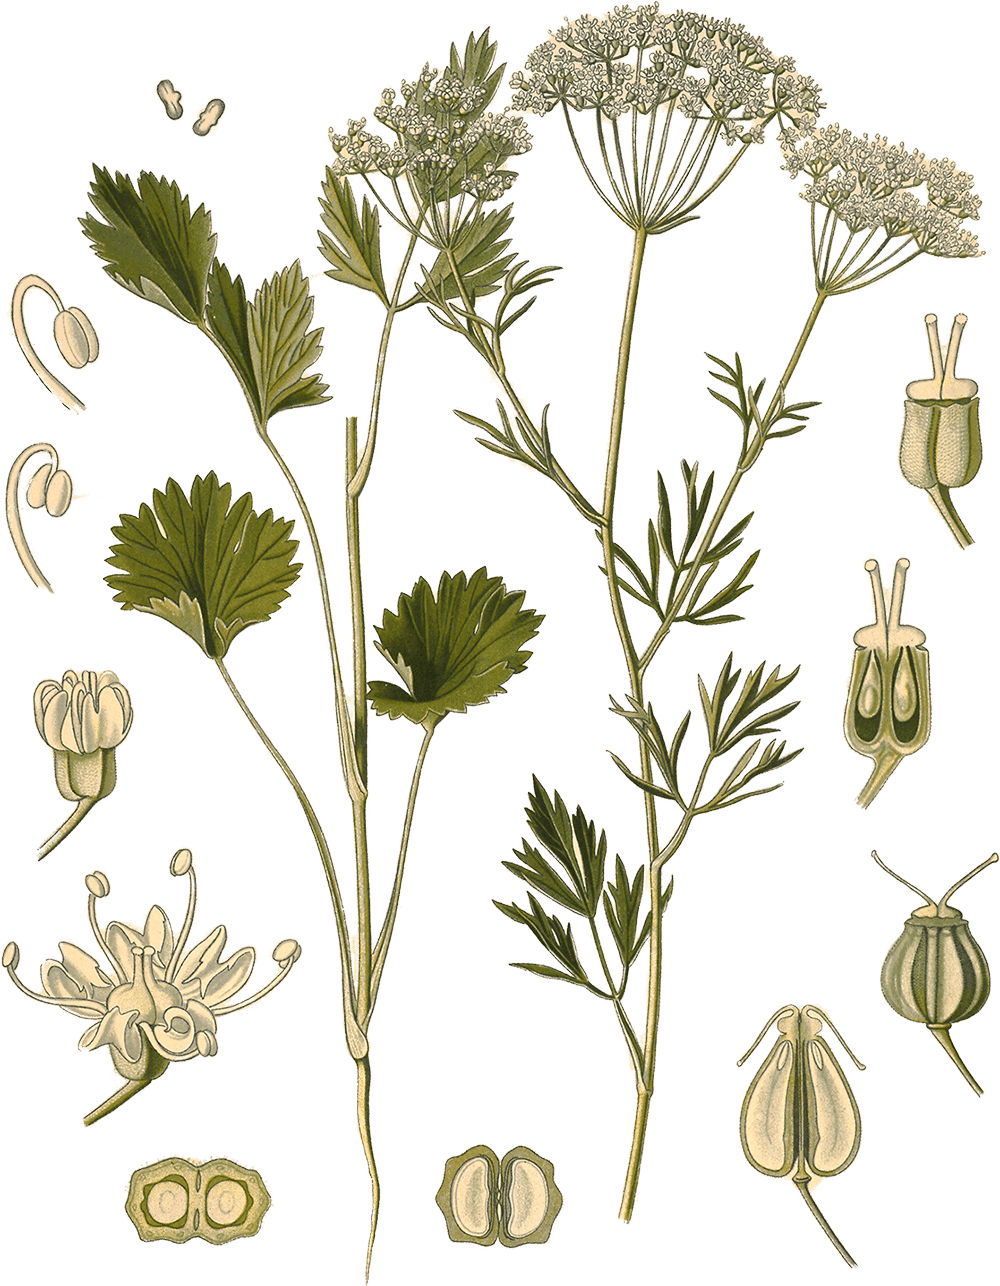
\includegraphics[width=\textwidth]{imgs/kohler/anise_kohler_min.png}
%     \caption{\taxonn{Pimenta dioica}{(L.) Merr.} (syn. \taxonn{P. officinalis}{ Lindl.}), the allspice tree in Köhler's Medicinal Plants \pvolcite[]{2}[174]{kohler_kohlers_1887}.}
%     \label{fig:kohler_anise}
% \end{figure}



\section{Anise}
\label{sec:anise}

\begin{spice}\label{spice:anise}
\textsc{Anise} \hfill \href{https://powo.science.kew.org/taxon/846658-1}{POWO} \\
\textbf{English:} \textit{anise}; \textit{aniseed}. 
\textbf{Arabic:} {\arabicfont{أنيسون}} \textit{anīsūn}; {\arabicfont{{يانسون} \textit{yānsūn}}}. 
\textbf{Chinese:} {\tradchinesefont{茴芹}} \textit{huíqín} [anise-celery]. 
\textbf{Hungarian:} \textit{ánizs}.  \\
\noindent{\color{black}\rule[0.5ex]{\linewidth}{.5pt}}
\begin{tabular}{@{}p{0.25\linewidth}@{}p{0.75\linewidth}@{}}
Plant species: & \taxonn{Pimpinella anisum}{L.} \\
Family: & \textit{Apiaceae} \\
part used: & fruit; oil \\
Region of origin: & E. Mediterranean; W. Asia \\
Cultivated in: & Turkey; Egypt; Spain; Russia; Italy; etc. \\
Color: & light brown \\
\end{tabular}
\end{spice}

% \begin{figure}[!ht]
% 	\vspace{-4ex}
% 	\centering
% 	\subfloat[\centering]{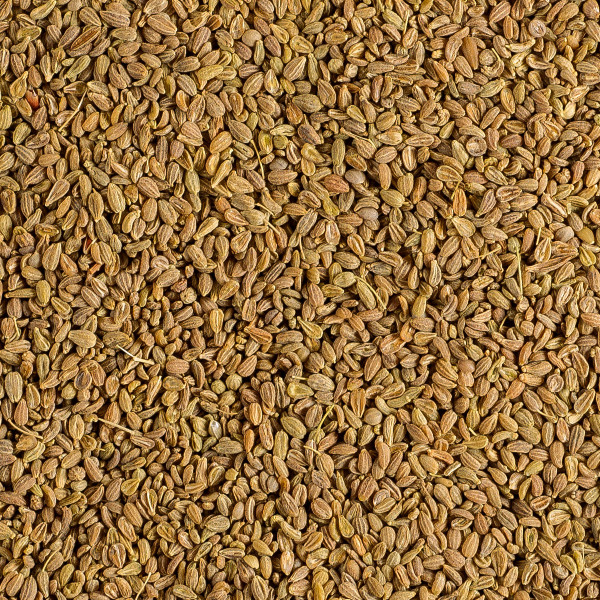
\includegraphics[width=0.3\linewidth]{imgs/spices/anise-1.jpg}}
% 	\hfill
% 	\subfloat[\centering]{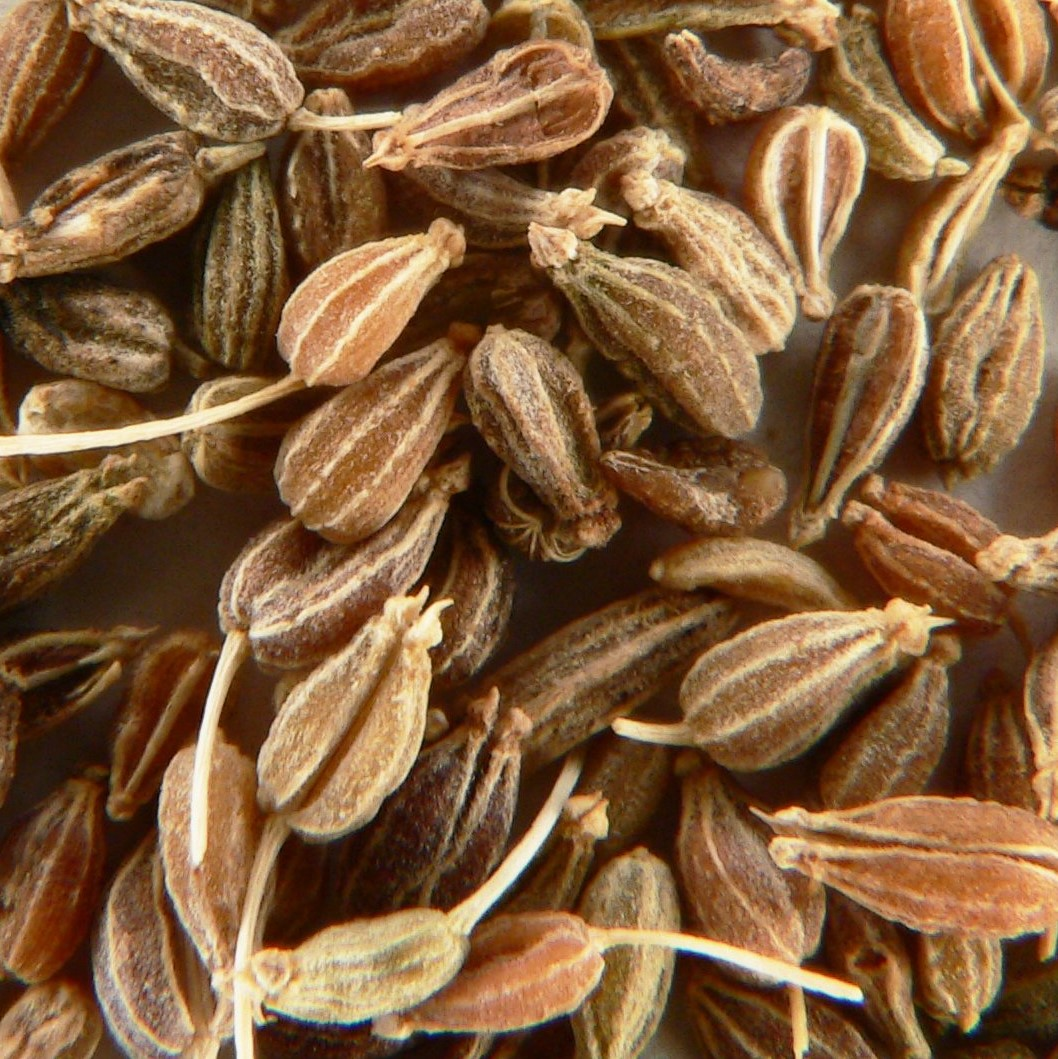
\includegraphics[width=0.3\linewidth]{imgs/spices/anise-11.jpg}}
% 	\hfill
% 	\subfloat[\centering]{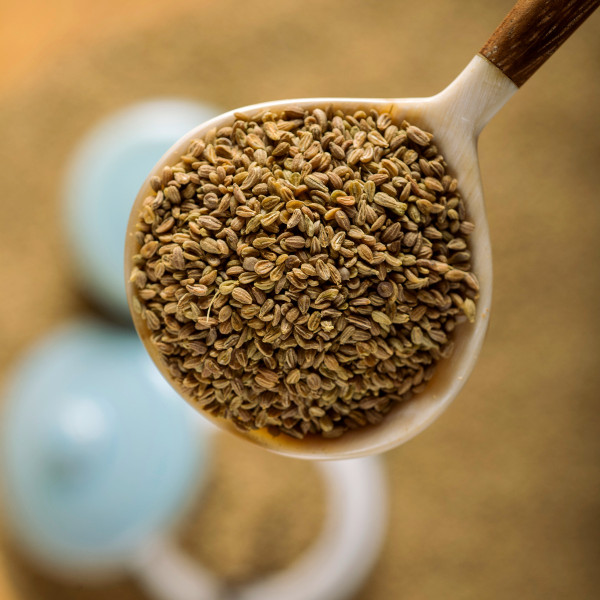
\includegraphics[width=0.3\linewidth]{imgs/spices/anise-3.jpg}}
% 	\caption{Anise \textit{Pimpinella anisum}.}
% 	\label{fig:anise_imgs}
% \end{figure}

\begin{wrapfigure}{R}{0.33\textwidth}
	\vspace{-\baselineskip}
	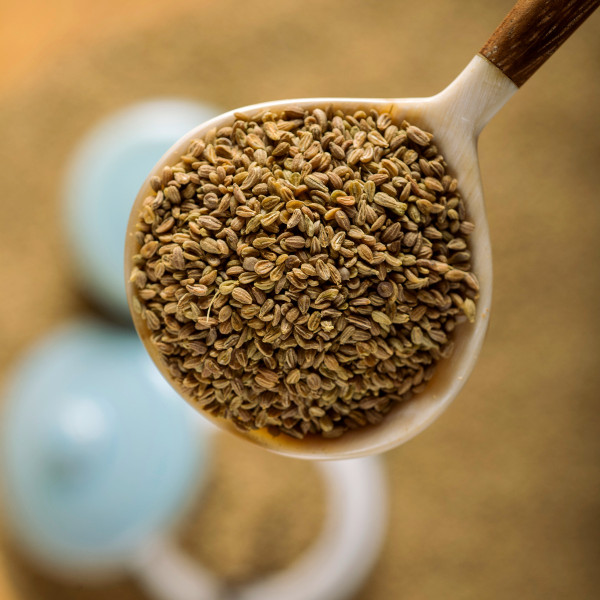
\includegraphics[width=0.33\textwidth]{imgs/spices/anise-s.jpg}
	\caption{Anise ``seeds'' (\textit{Pimpinella anisum}).}
	\label{fig:anise}
\end{wrapfigure}

%DESCRIPTION

Anise (\textit{Pimpinella anisum}) is a herbaceous plant, native to the Eastern Mediterranean and the Levant. It yields downy schizocarps,\footnote{Schizocarp refers to a dry compound fruit which splits into two or more one-seeded carpels (mericarps) without dehiscing} fruits which people call seeds. Hence the popular contracted form of the name, \textit{aniseed}. The seed-like fruits are grayish-green to light brown in color, and around 3--6 mm long \autocite[212]{van_wyk_culinary_2014}. Commercially available anise is usually sold whole, with a bit of stalk attached. Anise has visible \textit{vittae} (oil ducts) embedded in the fruit wall \pvolcite[]{2}[139]{peter_handbook_2012}, which is a feature similarly found on the fruits of related umbelliferous aromatic plants, such as fennel, cumin, caraway, carom/ajwain, and dill seeds.
Anise is sought after for its characteristic, liquorice-like sweet aroma and flavor, used in gastronomy, confectionery, and liqueur making -- especially around the Mediterranean. 
Anise and its essential oil is traditionally used as a flavoring for food, candy, and alcoholic drinks, however star anise oil from China has gradually replaced anise oil in the industry thanks to it being a much cheaper substitute \autocite[212]{van_wyk_culinary_2014}. % By 1999, world production in essential oil obtained from anise was 8 tons, while that of star anise was 400 \autocite{ashurst_food_1999}.

%OPERATIVE
The taste, smell, and even the appearance of anise resembles other---related and unrelated---spices, such as fennel, dill, liquorice, and star anise. This leads to a certain degree of confusion around the names which these plants and their products are known today in various languages. We will introduce this problem in more detail in \cref{sec:case_star_anise} in \nameref{ch:language}.

\begin{note}
	It is important to make the distinction between anise (\textit{Pimpinella anisum}) and star anise (\textit{Illicium verum}) from the beginning. These are two unrelated spices with distant origins. The similarities in name are due to their similarity in flavor, thanks to the organic compound anethole. 
	\end{note}

\subsection{The Botany, Origin, and  Cultivation of Anise}

%PLANT
Anise is an annual herb from the family \textit{Apiaceae/Umbelliferae}. Growing less than a meter tall, it brings small white flowers in umbels, the shape of an umbrella which is typical for this family of parsley, celery, and carrot. This family also contains many other aromatic flowering plants, such as asa\-foetida, coriander, cumin, caraway, dill, and fennel.

%ORIGIN
Anise originates in the Eastern Mediterranean region, growing from South East Turkey through Syria to the coasts of Lebanon, Israel, Palestine, and Egypt, including Cyprus, and in some sources also Greece. It has been cultivated since 2000 \BC{} \autocite[718]{mabberley_mabberleys_2017}.
%CULT
Anise today is naturalized in most of Europe and Central Asia, and it is cultivated as a crop in various regions around the globe, including, Southern Europe, Southern Russia, Turkey, the Middle East and North Africa, Pakistan, India, China, Chile, Mexico and the United States \autocite[32]{farrell_spices_1985}. It requires good soil, lots of sun and warmth, and also arduous to transplant. During harvest at summer's end when the fruits begin to ripen, the plant parts above ground are cut and the ``seeds'' are dried \autocite[212]{van_wyk_culinary_2014}.

\subsection{The History of Anise}

Anise has a long history around the Mediterranean, and its popularity is still concentrated there. It was used both as medicine an a culinary spice, as I mentioned above. The ancient Greeks took it as a breath freshener, and the Romans used it in their cooking \autocite{farrell_spices_1985}.

Pliny wrote a section of remedies with anise in his \textit{Natural History}, where he explains that it was recommended by Pythagoras to take with wine against scorpion stings, but it is also a great ingredient---both green and dried---in sauces and breads. And of course, it sweetens the morning breath with a little honey and smyrnion\footnote{\textit{Smyrnium olusatrum}, an edible pot herb commonly known as \textit{alexanders}} \autocite[20:72 \link{http://www.perseus.tufts.edu/hopper/text?doc=Perseus\%3Atext\%3A1999.02.0137\%3Abook\%3D20\%3Achapter\%3D72}]{pliny_the_elder_natural_1855}.

Medieval European herbals tell of carminative effect: ``The seed wasteth and consumeth winde, and is good against belchings and upbraidings of the stomach, alaieth gripings of the belly, provoketh urine gently, maketh abundance of milke, and stirreth up bodily lust: it staieth the laske (diarrhea), and also the white flux (leukorrhea) in women.'' \autocite[880 \link{https://www.gbif.org/species/113561272}]{gerarde_herball_1597}. Based on modern research, anise oil and anethole is antibacterial, antifungal, antioxidant, carminative, and expectorant \pvolcite[]{2}[144]{peter_handbook_2012}.

The Brits and Arabs use it since the Middle Ages. According to \textcite{wilson_wedding_2005}, 
the tradition of the wedding cake grew out of the customary spiced cakes at the end of feasts during Roman times, which served as digestive. In modern Europe, its use is prevalent in confectionery (such as aniseed balls), but especially liqueurs. From the many Mediterranean alcoholic beverages flavored with anise, we can mention anisette and absinthe (made with \textit{Artemisia absinthium}), from France, sambuca from italy, and ouzo and mastika from Greece. 
% ouzo effect
In the Eastern Mediterranean, it can be found in Turkish rakı, and the many araks of the Levant.

% USES
% culinary uses wyk
% Anise has a strong flavour and is used sparingly as a spice in soufflés, meat dishes (soups, stews, sausages), shellfish, vegetables (cabbage, carrots, turnips), mild cheeses, salad dressings, pickles, fruit dishes, desserts and juices. Chopped fresh leaves can be used in salads, pickled vegetables and fish soups. Star anise is nowadays often used as a substitute but connoisseurs say anise has a more delicate aroma. Anise is well known for its applications in confectionery (breads, biscuits, cakes and sweets) as well as alcoholic and non-alcoholic beverages. Examples of traditional culinary items and sweets are Australian humbugs, Austrian anisbögen, British aniseed balls, Dutch muisjes, German Pfeffernüsse and Springerle, Indian candy-coated saunf (used as mukhwas to freshen the breath after a meal), Italian pizzelle, New Mexican bizcochitos, New Zealand aniseed wheels, Norwegian knotts and Peruvian picarones. Well-known anise liqueurs or brandies/liquors (i.e., respectively with or without sugar) include French anisette, pastis and Pernod, Greek ouzo, Middle Eastern arrack, Italian sambuca, Spanish anís and Turkish raki. These are drunk with a glass of water on the side or more often directly diluted with water, resulting in the familiar ouzo effect (the drink becomes cloudy and milky because the alcohol-soluble anethole is no longer fully soluble and forms an emulsion). 

%Flavour compounds
%The fruits contain 1−4% essential oil with (E)-anethole, also referred to as trans-anethole, as the dominant compound (up to 90% or more) and several minor ingredients such as cis-γ-himachalene, trans-pseudoisoeugenyl 2-methylbutyrate, methylchavicol and p-anisaldehyde.3 Anethole is a phytoestrogen that also occurs in fennel. 

%notes In Pakistani and Indian cuisine, no distinction is made between anise and fennel – both are called saunf. In Southeast Asia, the name for star anise is sometimes shortened to anis.

% Mebberley:
% P. anisum L. (anise, Greece to Egypt) – cult. since 2000 BC, food& drink-flavouring subs. for Artemisia absinthium (absinthe, anis, anisette, arak, ouzo, pastis, raki), distilled oil medic., familiar as aniseed balls;

\subsection{The Names of Anise}

\textit{Anise} is a typical \gls{wanderwort}: emerging from moderately obscure origins, it is now ubiquitous to the languages of Europe and its sphere of influence where it is culturally significant.

\subsubsection{English}

\begin{etymology}\label{ety:anise}
English \textit{anise}, ca. 1325
< French \textit{anis} `anise', 1236
< Latin \textit{anīsum} `anise', (dill is \textit{anēthum})
< Ancient Greek {ἄνισον} \textit{ánison} `anise; dill', and other Greek dialectal variants, e.g.: \textit{ánēthon}; included both plants, only later distinguished (probaby of substrate origin)
<\textss{?} Egyptian (Ancient) \textit{jnst} `a medicinal, edible plant (probably anise)'\footnote{\textcites[anise]{oed}[anise]{ahd}; \textcite[s.v. anis]{tlfi}; \textcite{lewis_latin_1879}; \textcite{liddell_greek-english_1940}; \textcites[99]{erman_worterbuch_1926}[240]{hemmerdinger_noms_1968}}
\end{etymology}

To English, it arrived in the \nth{14} century via French \textit{anis}, which descended from Latin \textit{anīsum}. The Latin word is a borrowing from Ancient Greek ἄνισον \textit{ánison}, which is attested in different forms in various Greek dialects of the time, sometimes with \textit{-nn-} and theta instead of sigma (e.g.,ἄνηθον \textit{anēthon}). We can often read that this word originally referred to dill, but it seems that the Greeks did not distinguish between the two, and the terms included both plants.\footcite[anise]{oed} Hence the scientific name of dill: \textit{Anethum graveolens}. According to \textcite[103,107]{beekes_etymological_2010}, \textit{ánison} is anise, while \textit{anēthon} is dill, but he points out that they probably have the same etymon. The Romans borrowed both words, and the distinction was made explicit in \textit{anīsum} vs. \textit{anēthum}. The modern scientific names bear the Latin names: \textit{Pimpinella anisum} (anise), where meaning of \textit{pimpinella} is uncertain, and \textit{Anethum graveolens} (dill), where \textit{graveolens} means `strong scented' \autocite[184,303]{gledhill_names_2008}. The confusion of the Greek words had an effect on English much later as well, in Matthew 23:23 of the \gls{KJV}\footnote{Source: \url{https://www.biblegateway.com/passage/?search=Matthew+23\%3A23&version=KJV}} talks of anise, while newer, more accurate translations, such as the \gls{NRSV}\footnote{Source: \url{https://www.biblegateway.com/passage/?search=Matthew+23\%3A23&version=NRSVUE}} mention dill. In fact, one of the first attestation in English comes from Wycliffe's Bible in 1382, between mint and cumin: ``That tithen mente, anete [anese], and comyn.''\footcite[anise]{oed} Beyond Greek, the etymology of this word is uncertain, \textcite[103,107]{beekes_etymological_2010} suspects a pre-Greek, substrate origin demonstrated by the phonological variations. Although the \citetitle{erman_worterbuch_1926} in an early Egyptian glossary makes a connection with the Egyptian word rendered as \textit{jnst}\footnote{Transliterated as \textit{ꞽnś.t} in \textcite[99]{erman_worterbuch_1926}, conventional Egyptological pronunciation: /insɛt/} `an edible plant for medicinal use' in the literature of the Middle Kingdom, the assumption is marked with question marks in the original handwritten glossary \autocites[240]{hemmerdinger_noms_1968}[99]{erman_worterbuch_1926}. The \gls{AHD} remarks that the Greek word is ``perhaps from or akin'' to Egyptian \textit{ꞽnśt}---using a different transliteration---which is a kind of plant used in the preparation of refreshing drinks, possibly anise.\footcite[anise \link{https://www.ahdictionary.com/word/search.html?q=anise}]{ahd} 

% An association between dill and the ancient city of Imsety has been made due to the similarity of their names in Old Egyptian. Redford 1:562; more about jnst in Wiktionary

The idea is not far-fetched, anise, dill and other herbs are native to the region and were ``almost surely grown'' for their medicinal properties \pvolcite[]{2}[3]{redford_oxford_2001}. We know that spices and herbs were used to flavour Ancient Egyptian cooking, Egyptologists have identified indigenous ingredients (dill, fenugreek, parsley, thyme, nigella, fennel, marjoram, mint), those imported and transplanted from neighboring Palestine (dill, cumin, coriander, caraway) and those obtained through distant trade (cinnamon and peppercorns from Asia) by the wealthy, later during the New Kingdom times \pvolcite[]{1}[394,540]{redford_oxford_2001}.

Anise is also known as \textit{aniseed}, which is a contraction from \textit{anise} and \textit{seed}, a usage form that emerged in the late \nth{14} century. 

\textit{Sweet cumin} is another conventional name for anise, which shows the primacy of the word \textit{cumin} in English, when it comes to similar aromatic plants and their seeds. Cf. \textit{wild cumin}, \textit{Armenian cumin}, \textit{mountain cumin} (caraway); royal cumin\footnote{Parallel to Indo-Persian \textit{sh\={a}h-j\={i}r\={a} [king-cumin] `caraway'}} (bishop's weed), and the always ambiguous \textit{black cumin}

\begin{table}[!ht]
\centering
\begin{tabularx}{\textwidth}{@{}l>{\itshape \small}lL>{\small}l@{}}
\toprule
\textbf{\#} & \multicolumn{1}{l}{\textbf{Species}} & \multicolumn{1}{l}{\textbf{Name}} & \multicolumn{1}{l}{\textbf{Source}} \\
\midrule
\textbf{1}	& \textbf{Pimpinella anisum}	& \textbf{anise}	& \textbf{\textcite{van_wyk_culinary_2014}} \\
2	& Pimpinella anisum	& aniseed	& \textcite{van_wyk_culinary_2014} \\
3	& Pimpinella anisum	& sweet cumin	& \textcite{peter_handbook_2012} \\
\bottomrule
\end{tabularx}
\caption{Various names for anise in English.}
\label{table:names_anise_en}
\end{table}



\subsubsection{Arabic}

\begin{etymology}\label{ety:anisun}
Arabic {أنيسون} \textit{anīsūn} `anise', (later assimilated as \ar{يانسون} \textit{yānsūn}), a. 791
< Ancient Greek {ἄνισον} \textit{ánison} `anise; dill', and other Greek dialectal variants, e.g.: \textit{ánēthon}; included both plants, only later distinguished (probaby of substrate origin)
<\textss{?} Egyptian (Ancient) \textit{jnst} `a medicinal, edible plant (probably anise)', ca. 2030-1650 BC\footnote{\textcite{wehr_dictionary_1976}; \textcite{liddell_greek-english_1940}; \textcites[99]{erman_worterbuch_1926}[240]{hemmerdinger_noms_1968}}
\end{etymology}

In Arabic, similarly to English, the name of anise is a loanword from Greek. It is known by many spelling variations: \textit{anīsūn}, \textit{ānīsūn}, \textit{ansūn}, \textit{yānsūn}, and \textit{yansūn}. In general, the \textit{a-} forms were the initial loanword taken directly from Greek, then a \textit{y-} form emerged that assimilates better in Arabic phonology. In addition, synonyms for anise are \textit{kammūn ḥulw}, lit. `sweet cumin', and \textit{ḥubba ḥulwa} `sweet grain, sweet seed'.

Anise in Persian, is \fa{بادیان رومی} \textit\textit{bādyān rūmī}\footcite[Vol. 1, p. 197]{hayyim_new_1934}, literally `Roman anise', where \textit{bādyān} is an archaic word for either fennel or anise, the etymon of French \textit{badiane} that begot English \textit{badian} `star anise'. A possible connection between Persian \textit{bādyān} and Mandarin Chinese \tc{八角} \textit{bajiao} `star anise' have been proposed before, % by who
but in my opinion this is merely wishful thinking.

\begin{table}[!ht]
\centering
\begin{tabularx}{\textwidth}{@{}l>{\itshape \small}lr>{\itshape}lL>{\small}l@{}}
\toprule
\textbf{\#} & \multicolumn{1}{l}{\textbf{Species}} & \multicolumn{1}{l}{\textbf{Name}} & \multicolumn{1}{l}{\textbf{Tr.}} & \multicolumn{1}{l}{\textbf{Gloss}} & \multicolumn{1}{l}{\textbf{Source}} \\
\midrule
\textbf{1}	& \textbf{Pimpinella anisum}	& \textbf{أنيسون}	& \textbf{anīsūn}	& \textbf{phonetic}	& \textbf{\textcite{wehr_dictionary_1976}} \\
2	& Pimpinella anisum	& كمون حلو	& kammūn ḥulw	& sweet cumin	& \textcite{wehr_dictionary_1976} \\
3	& Pimpinella anisum	& يانسون	& yānisūn	& phonetic	& \textcite{wehr_dictionary_1976} \\
4	& Pimpinella anisum	& حبة حلوة	& ḥabba ḥulwa	& sweet grain, seed	& \textcite{wehr_dictionary_1976} \\
\bottomrule
\end{tabularx}
\caption{Various names for anise in Arabic.}
\label{table:names_anise_ar}
\end{table}



\subsubsection{Chinese}

\begin{etymology}\label{ety:huiqin}
Mandarin Chinese {茴芹} \textit{huíqín} `anise' [hui-celery], from \textit{hui} `anise/fennel' + \textit{qin} `celery' (茴 \textit{huí} could be interpreted as `Muslim spice', see 茴香 \textit{huíxiāng} `fennel'), 1841\footnote{\textcite{kleeman_oxford_2010; hu_food_2005}}
\end{etymology}

The gathering of names for anise is a bit difficult in Chinese for two reasons. Firstly, anise as a spice is relatively unknown in China except for Xinjiang, and therefore names are hard to find in sources. Since other spices with a similar flavour profile, such as the native star anise and the naturalized fennel are readily available, so anise was never imported into China. Consequently, we cannot find anise in reference works on Chinese food plants nor in Chinese \gls{materia medica} \autocite[see][]{hu_enumeration_1999, hu_food_2005}. It does however appear in the \gls{FOC}\footnote{Source: \url{http://www.efloras.org/florataxon.aspx?flora_id=2&taxon_id=200015767}} Secondly, identifications is problematic and confusing due to the mixing of terms \textit{anise}, \textit{aniseed}, \textit{star anise}, \textit{star aniseed}, etc. in English, and Chinese dictionaries, and in some databases as well. Dictionaries that do not give botanical names are of little help to clarify doubts, but some conclusions can be derived with care. Most dictionary entries in Chinese that translate \textit{anise} to \textit{aniseed} should in fact say \textit{star anise}, as they ar all words referring to the Asian spice, except for one: \tc{茴芹} \textit{huiqin}.

Anise in Chinese is 茴芹 \textit{huiqin} `anise-celery', which appears to be a relatively modern, scientific coinage, and the only \gls{phytonym} that appears in any publication (the \gls{FOC}). It is used in the strict sense of \textit{Pimpinella anisum} and cannot be misunderstood for star anise (\textit{Illicium verum}). It does not appear in historical corpora, and it is not included in the \nth{7} edition of the \textit{Xiandai Hanyu Cidian} [A Dictionary of Modern Chinese] \autocite[]{chinese_academy_of_social_sciences_xiandai_2016}, but it appears in the \gls{CEC}\footnote{Source: \url{https://dictionary.cambridge.org/dictionary/english-chinese-traditional/anise} and \url{https://dictionary.cambridge.org/dictionary/english-chinese-traditional/aniseed}.}, which gives us \textit{huiqin}, along with \tc{洋茴香} \textit{yanghuixiang} `Western anise'. \tc{茴香} \textit{huixiang} really refers to fennel, and the only reason it appears in \textcite{kleeman_oxford_2010} is the confusion between the materials, and their names. The nomenclature and the reasons behind its confusion will be explored in more detail in \cref{sec:case_star_anise}. A few other names are mentioned on the Chinese Wikipedia page of the plant, these all refer to the European origins of this spice, or referring to``Western Ocean'', the Indian Ocean used to denote foreign, western products that have arrived over sea.\footnote{Source: \url{https://zh.wikipedia.org/wiki/\%E8\%8C\%B4\%E8\%8A\%B9}}. 

A Latin-Chinese dictionary from a presbyterian missionary from 1841 lists \textit{huiqin} as \textit{thymus} `thyme',\footcite[715]{goncalves_lexicon_1841} which is rather confusing considering that 10 years earlier, the same author rendered it `oregano' in his Portuguese-Chinese dictionary.\footcite[585]{goncalves_diccionario_1831}. From this, we can speculate that more of the various spice herbs that the Portuguese and other Europeans brought to Macao were first denoted with \textit{huiqin}.

% oregano in 
% https://books.google.com.hk/books?id=BYE-AQAAIAAJ&pg=PA585&dq=%22%E8%8C%B4%E8%8A%B9%22&hl=en&sa=X&ved=2ahUKEwi1xs7slpb5AhWJet4KHe9NCicQ6AF6BAgEEAI#v=onepage&q=%22%E8%8C%B4%E8%8A%B9%22&f=false

% thyme in
% https://books.google.com.hk/books?id=rOBoAAAAcAAJ&pg=PA715&dq=%22%E8%8C%B4%E8%8A%B9%22&hl=en&sa=X&ved=2ahUKEwi1xs7slpb5AhWJet4KHe9NCicQ6AF6BAgJEAI#v=onepage&q=%22%E8%8C%B4%E8%8A%B9%22&f=false

\begin{table}[!ht]
\centering
\begin{tabularx}{\textwidth}{@{}l>{\itshape \small}ll>{\itshape}lL>{\small}l@{}}
\toprule
\textbf{\#} & \multicolumn{1}{l}{\textbf{Species}} & \multicolumn{1}{l}{\textbf{Name}} & \multicolumn{1}{l}{\textbf{Tr.}} & \multicolumn{1}{l}{\textbf{Gloss}} & \multicolumn{1}{l}{\textbf{Source}} \\
\midrule
\textbf{1}	& \textbf{Pimpinella anisum}	& \textbf{\tradchinesefont{茴芹}}	& \textbf{huíqín}	& \textbf{hui-celery}	& \textbf{\textcite{kleeman_oxford_2010}} \\
2	& Pimpinella anisum	& \tradchinesefont{茴香}	& huíxiāng	& hui-spice	& \textcite{kleeman_oxford_2010} \\
3	& Pimpinella anisum	& \tradchinesefont{西洋茴香}	& xīyánghuíxiāng	& western-ocean-hui-spice	& \textcite{wikipedia} \\
4	& Pimpinella anisum	& \tradchinesefont{洋茴香}	& yánghuíxiāng	& ocean-hui-spice	& \textcite{cec} \\
5	& Pimpinella anisum	& \tradchinesefont{歐洲大茴香}	& ōuzhōu dàhuíxiāng	& European-big-hui-spice	& \textcite{wikipedia} \\
\bottomrule
\end{tabularx}
\caption{Various names for anise in Chinese.}
\label{table:names_anise_zh}
\end{table}



\subsubsection{Summary}

\Cref*{table:names_anise} shows the names of anise that can be found in dictionaries.

\begin{table}[!ht]
\centering
\begin{tabularx}{\textwidth}{@{}ll>{\itshape}lLl>{\small}l@{}}
\toprule
\textbf{\#} & \textbf{Language} & \multicolumn{1}{l}{\textbf{Term}} & \textbf{Gloss} & \textbf{Loan} & \multicolumn{1}{l}{\textbf{Source}} \\
\midrule
1	& English	& anise	& 	& yes	& \textcite{oed} \\
2	& English	& aniseed	& 	& no	& \textcite{oed} \\
3	& English	& sweet cumin	& 	& no	& \textcite{oed} \\
\midrule
1	& Arabic	& anīsūn	& phonetic	& yes	& \textcite{wehr_dictionary_1976} \\
2	& Arabic	& kammūn ḥulw	& sweet cumin	& no	& \textcite{wehr_dictionary_1976} \\
3	& Arabic	& yānisūn	& phonetic	& yes	& \textcite{wehr_dictionary_1976} \\
4	& Arabic	& ḥabba ḥulwa	& sweet grain, seed	& no	& \textcite{wehr_dictionary_1976} \\
\midrule
1	& Chinese	& huíqín	& hui-celery	& no	& \textcite{kleeman_oxford_2010} \\
2	& Chinese	& huíxiāng	& hui-spice	& no	& \textcite{kleeman_oxford_2010} \\
\bottomrule
\end{tabularx}
\caption{Conventionalized names for anise in English, Arabic, and Chinese, found in dictionaries.}
\label{table:names_anise}
\end{table}













%==========================================

% EE:
% umbelliferous plant with aromatic seeds. XIV. — (O)F. anis :- L. ánīsum — Gr. ānīson.
% Hence aniseed XIV (anece seed).

% OE:
% anise (n.)
% Levantine plant cultivated for its seeds, which were important sources of chemical oils and flavoring, c. 1300, from Old French anis (13c.), from Latin anisum, from Greek anison. By the Ancients somewhat confused with dill. Related: Anisic.
% Entries linking to anise
% aniseed (n.)
% late 14c., a contraction of anise seed (n.).
% anisette (n.)
% "liqueur flavored with aniseed," 1821, from French Anisette de Bordeaux, from diminutive of anis (see anise).

% MW:
% Middle English anis, from Old French, from Latin anisum, anesum, from Greek anison, anēson
% First Known Use: 14th century (sense 1)

% AH:
% [Middle English anis, from Old French, from Latin anīsum, from Greek annēson, annīson, anīson; akin to anēthon, annēthon, dill, and perhaps from or akin to Egyptian jnś.t, a kind of plant used in preparing refreshing drinks (possibly anise).] 

% WK:
% From Middle English anys, borrowed from Old French anis, from Latin anīsum, from Ancient Greek ἄνισον (ánison), from Egyptian jnst. 

\clearpage % % Full page illustration
% \begin{figure}[!hbtp]
%     \centering
%     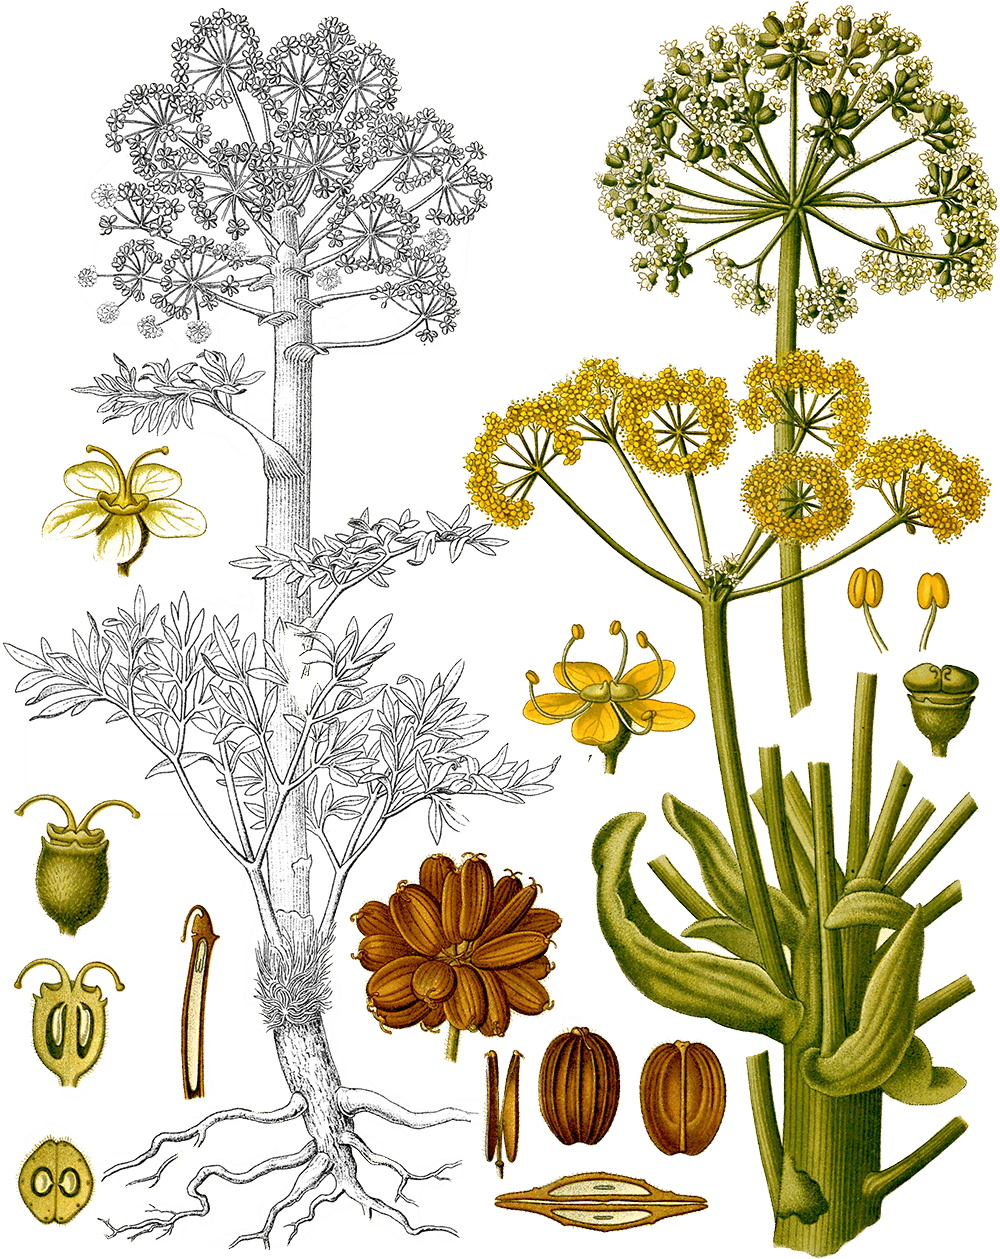
\includegraphics[width=\textwidth]{imgs/kohler/asafoetida_kohler_min.png}
%     \caption{\taxonn{Ferula foetida}{(Bunge) Regel} (syn. \taxonn{Ferula scorodosma}{Benth. \& Hook.}), one of the sources of asafoetida in Köhler's Medicinal Plants \pvolcite[]{2}[147]{kohler_kohlers_1887}.}
%     \label{fig:kohler_asafoetida}
% \end{figure}



\section{Asafoetida}
\label{sec:asafoetida}

\begin{spice}\label{spice:asafoetida}
\textsc{Asafoetida} \hfill \href{https://powo.science.kew.org/taxon/842277-1}{POWO} \\
\textbf{English:} \textit{asafoetida}; \textit{hing; devil's dung}. 
\textbf{Arabic:} {\arabicfont{حلتیت}} \textit{ḥiltīt}. 
\textbf{Chinese:} {\tradchinesefont{阿魏}} \textit{āwèi}. 
\textbf{Hungarian:} \textit{ördöggyökér} [devil's root]; \textit{aszatgyanta} [asat resin]; \textit{bűzös aszat} [stinking asat].  \\
\noindent{\color{black}\rule[0.5ex]{\linewidth}{.5pt}}
\begin{tabular}{@{}p{0.25\linewidth}@{}p{0.75\linewidth}@{}}
Plant species: & \taxonn{Ferula foetida}{(Bunge) Regel}; \textit{\taxonn{Ferula assa-foetida}{L.}; \textit{Ferula narthex}; et al.} \\
Family: & \textit{Apiaceae} \\
part used: & gum-resin (latex) \\
Region of origin: & Iran; W. and C. Asia \\
Cultivated in: & Iran; Afghanistan \\
Color: & from pale yellow to brown \\
\end{tabular}
\end{spice}

\begin{figure}[!ht]
	\vspace{-4ex}
	\centering
	\subfloat[\centering gum-resin ]{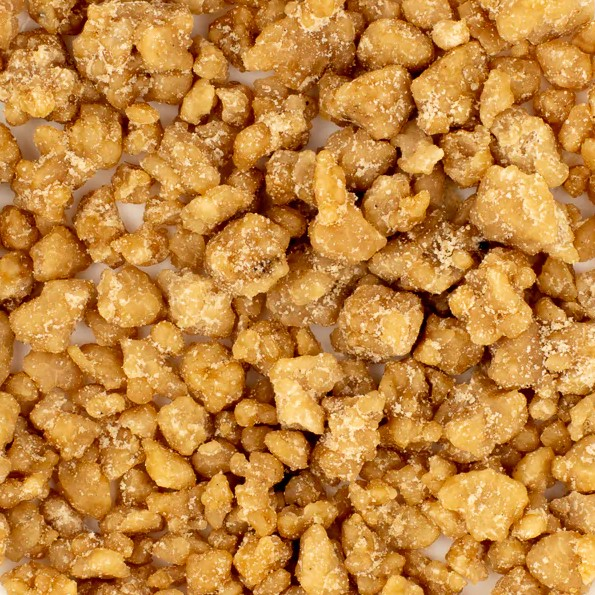
\includegraphics[width=0.3\linewidth]{imgs/spices/asafoetida-1.jpg}}
	\hfill
	\subfloat[\centering powder, colored with turmeric]{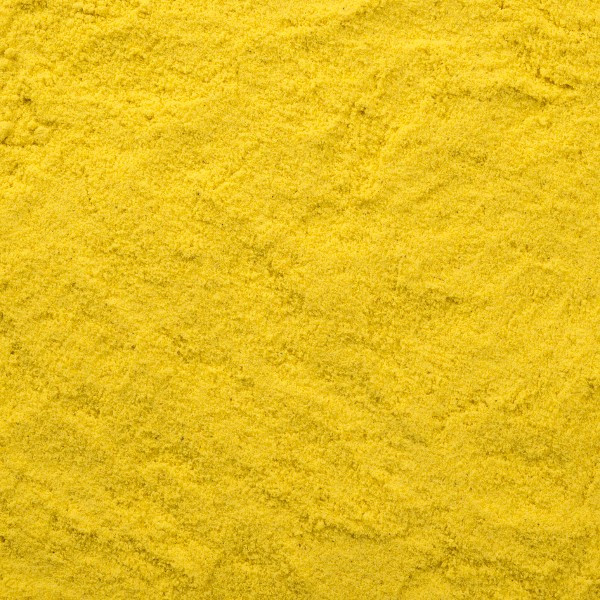
\includegraphics[width=0.3\linewidth]{imgs/spices/asafoetida-2.jpg}}
	\hfill
	\subfloat[\centering plant]{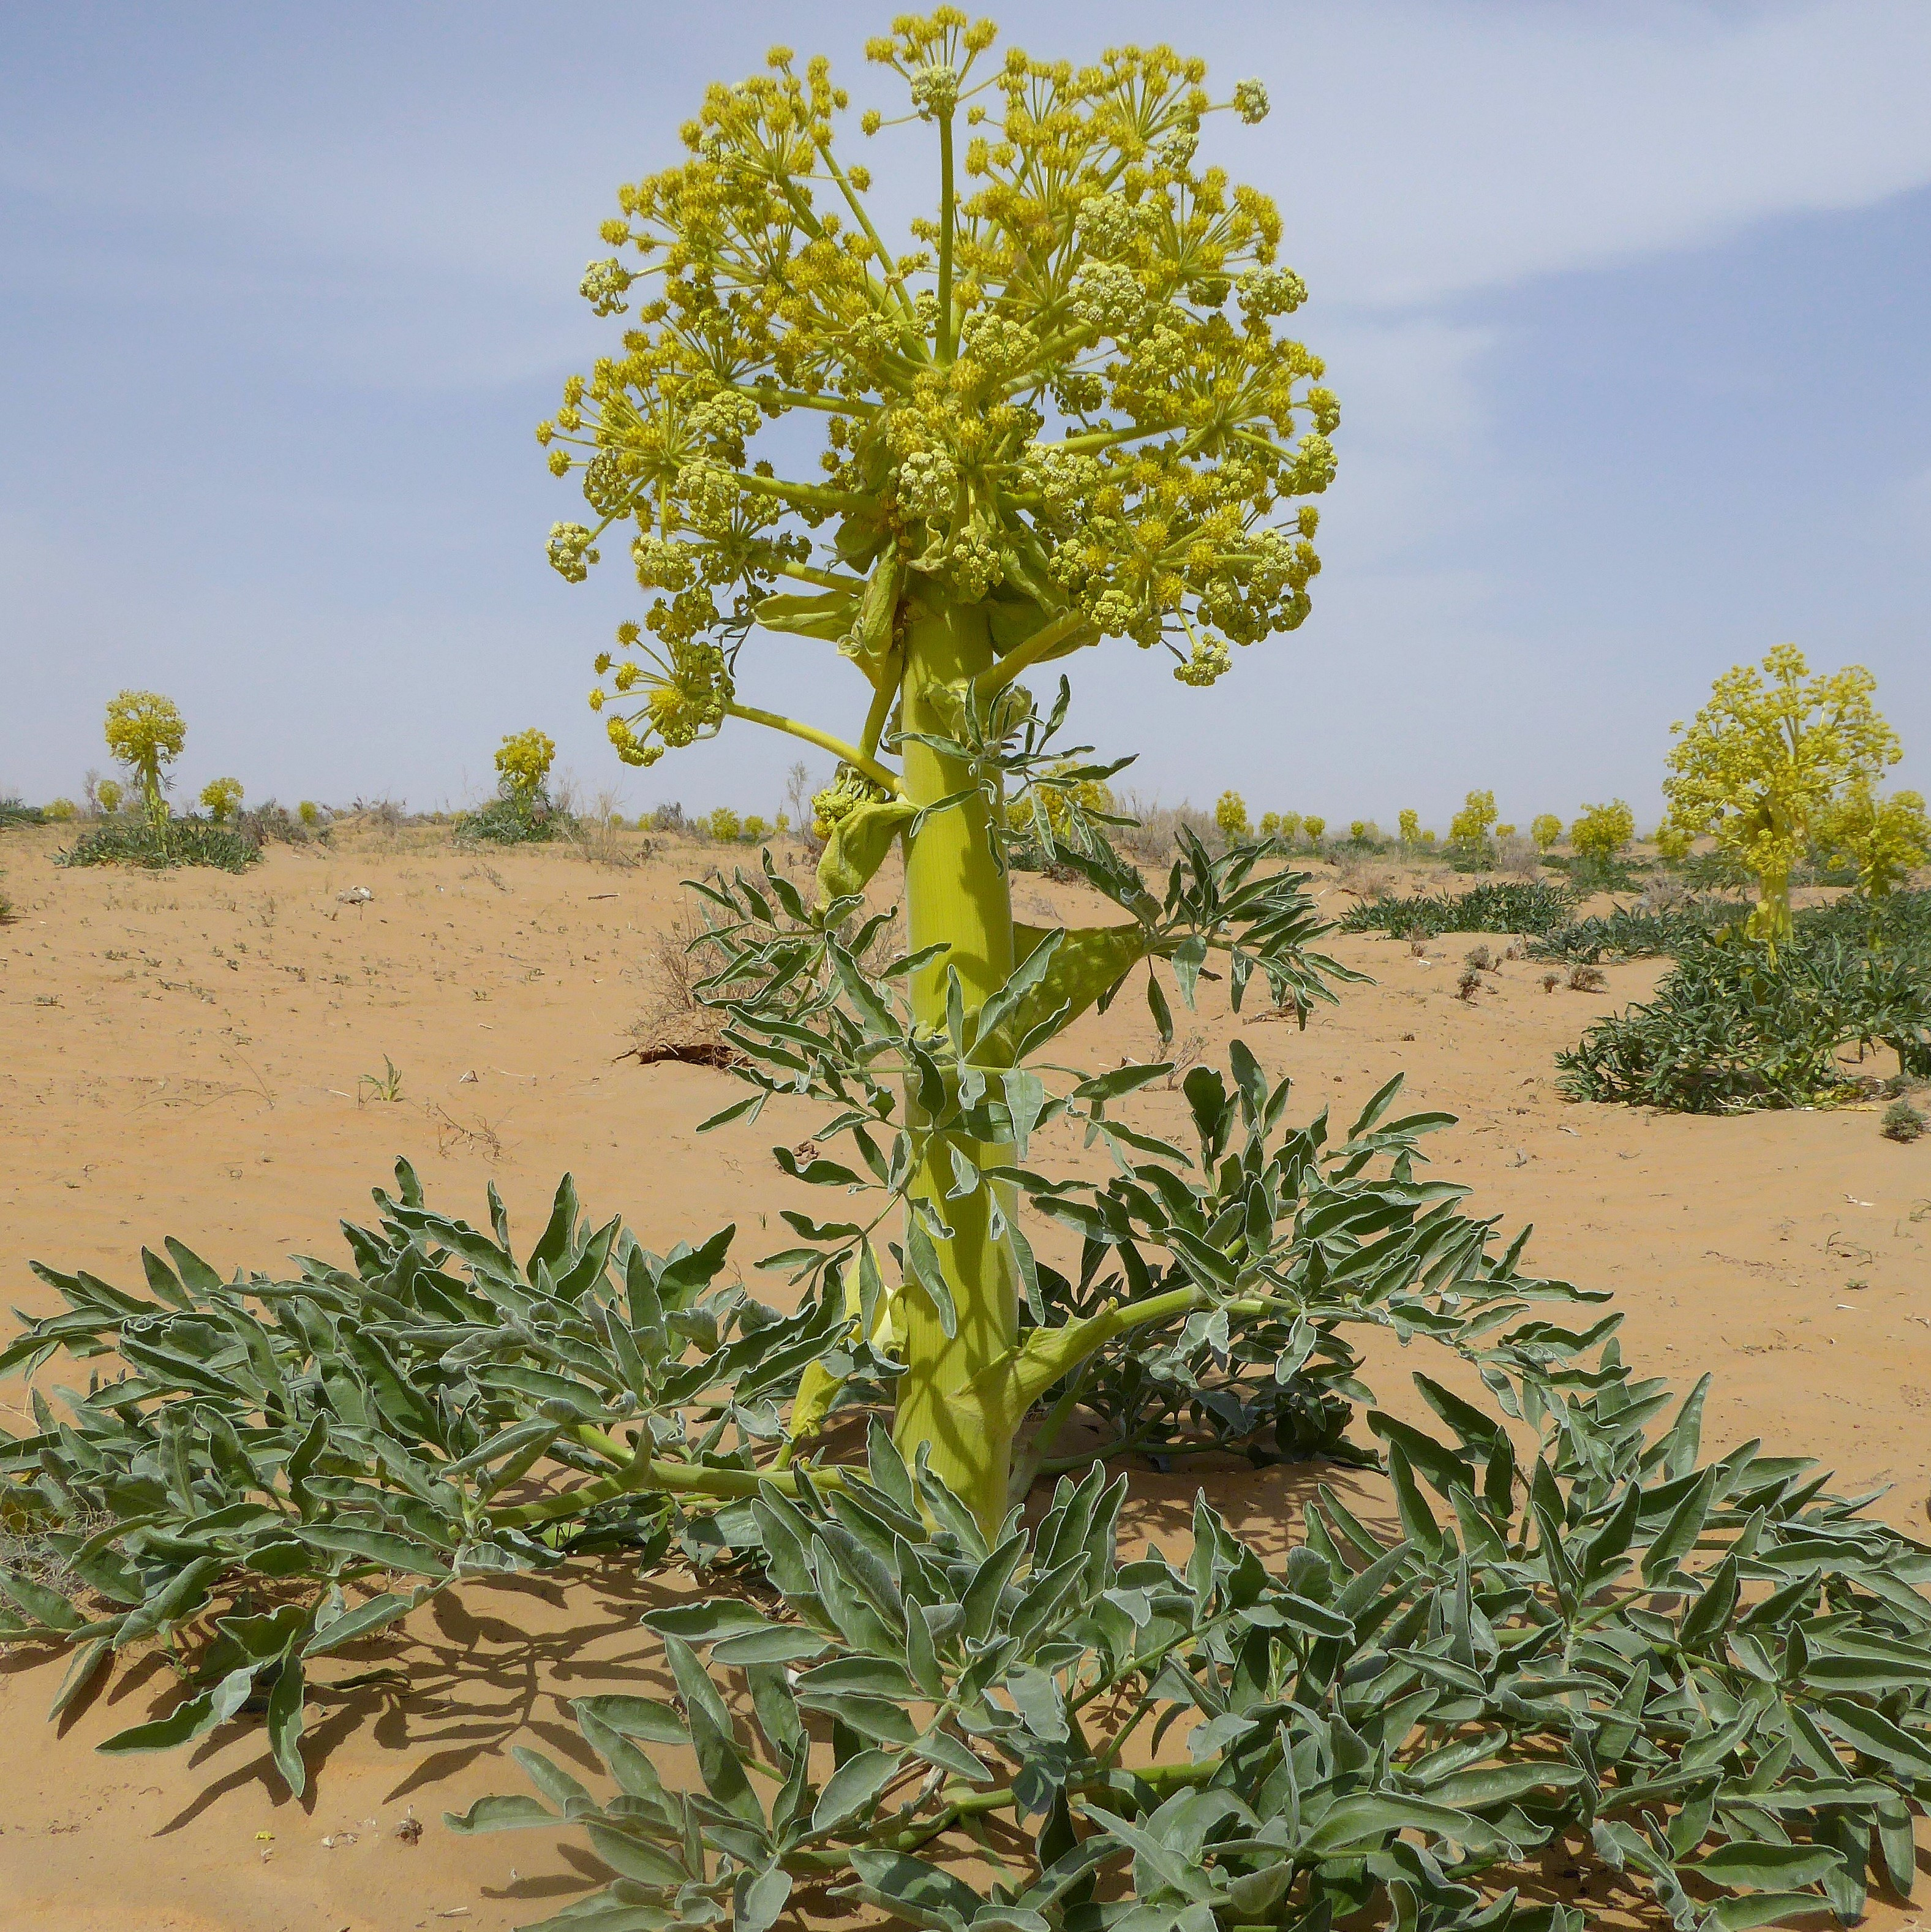
\includegraphics[width=0.3\linewidth]{imgs/spices/asafoetida-3.jpg}}
	\caption{Asafoetida in various forms, and one of its principal sources \taxon{Ferula assa-foetida} in the Kyzylkum Desert. Credit: Glorian; Aromatique; Public Domain}
	\label{fig:asafoetida_imgs}
\end{figure}

Asafoetida is the dried, golden brown oleoresin that forms after cutting the stems of various ferula plants of Central Asia. The material itself is a waxy gum-resin, and it is sold either in gum or powdered form. Asafoetida is an extremely pungent, strong-smelling substance; it is described having a ``garlic-like'' and ``sulphurous odor'' that is sometimes too strong in itself and must be diluted with other materials \autocite[138]{van_wyk_culinary_2014}. Asafoetida is a drug and spice, and was used for centuries in both Asia and Europe \autocite{leung_itinerary_2019}. It is still an integral part of Indian cuisine as an ingredient, while in Europe and East Asia it was mainly utilized as medicine.

Regarding the characteristics and uses of the plant asafoetida, there are parallels with the now extinct giant ferula plant, which is believed to be the source of the lost silphium or laserpitium of antiquity. Silphium was a drug used in ointments of traditional Greek medicine, and a coveted ingredient in Roman cuisine. It was and introduced from Libya in North Africa, and was once a commercially crucial product featured on Roman coins. We now believe that over-harvesting led to its demise \autocites{dalby_dangerous_2000, leung_itinerary_2019, van_wyk_culinary_2014, langenheim_plant_2003}. 

\subsection{The Botany, Origin, and  Cultivation of Asafoetida}

%PLANT
Asafoetida is obtained from species of the genus \textit{Ferula} in the \textit{Apiaceae} family, such as \taxon{Ferula assa-foetida}, \taxon{F. foetida}, and \taxon{F. narthex} \autocite{mabberley_mabberleys_2017}. These plants are ``robust perennial herbs'' that can grow to 2 m high, and as umbelliferous plants surmounted by large yellow flowers \autocite[138]{van_wyk_culinary_2014}.
%ORIGIN
The plants cope well in mountainous and dry, desert-like conditions of Iran (from Yazd to Lar), up to Southern Uzbekistan (Kyzylkum Desert), and the Qandahar region of Afghanistan where they grow wild \autocite{leung_itinerary_2019}.
%CULT
Asafoetida is wild-harvested the same way it has been for thousands of years. The plant is cut before flowering, at the base of the stalk just above the root, and left exposed. The exudate is then collected once it solidifies, and this process is repeated again and again for up to three months, until no more liquid can be tapped \autocite[138]{van_wyk_culinary_2014}.

% culinary uses 
% Asafoetida is an important spice in Middle Eastern and South Asian cuisines and is widely used (especially in India) to flavour meat dishes, stews, gravies, sauces, mushrooms and pickles. When used sparingly, the offensive smell is lost during cooking, leaving a pleasant, garliclike aroma. The spice is not popular in Western cuisine but is (or was) allegedly an essential ingredient of Worcestershire sauce. 

% Used like onion or garlic.
% It was used by Jains and Brahmins because they do not eat onion! ??

% Flavour compounDs 
% The gum or oleoresin is a complex mixture of compounds, including ferulic acid esters, polysaccharide gums based on glucose, galactose and galacturonic acids, as well as terpenoids and coumarins.4,5 The odour is ascribed to various sulphides and sulfanes; secbutyl-propenyl disulphide (both E and Z isomers) are usually the main sulphur compounds.4,5 


% 1. Mabberley, D.J. 2008. Mabberley’s plant-book (3rd ed.). Cambridge University Press, Cambridge. 
% 2. Langenheim, J.H. 2003. Plant resins, pp. 412–417. Timber Press, Portland. 
% 3. Chamberlain, D.F. 1977. The identity of Ferula assa-foetida L. Notes from the Royal Botanic Garden, Edinburgh 35: 229–233. 
% 4. Rajanikanth, B., Ravindranath, B., Shankaranarayana, M.L. 1984. Volatile polysulphides of asafoetida. Phytochemistry 23: 899–900. 
% 5. Degenhardt, A. et al. 2012. Novel insights into the flavour chemistry of asafetida. In: Recent advances in the analysis of food and flavors, Chapter 12, pp. 167–175. American Chemical Society.

%  Teufelsdreck in German.

\subsection{The History of Asafoetida}

A fantastic chapter on the history of asafoetida already exists \citetitle{leung_itinerary_2019} by \textcite{leung_itinerary_2019} 

\subsection{The Names of Asafoetida}

\subsubsection{English}

\begin{etymology}\label{ety:asafoetida}
\textbf{English} \textit{asafoetida}, a. 1398
< \textbf{Medieval Latin} \textit{asafoetida} [stinking asa]
<\textss{?} from \textbf{Persian} \textit{āzā} `mastic', in a Lanized form, \textit{asa}
 + \textbf{Latin} \textit{foetid} `ill-smelling, stinking', (feminine of \textit{fœtidus})\footnote{\textcite[s.v. asafoetida]{oed}; \textcite[353]{laufer_sino-iranica_1919}; \textcite[42]{steingass_comprehensive_1892}}
\end{etymology}

\textit{Asafoetida} \amarginpar{asafoetida} (also spelled \textit{asafetida}) is a term directly from Medieval Latin that found its way into the English lexicon via the early modern European medicinal and botanical literature. Often seen with archaic spellings, such as \textit{``assafœtida''}, the name is made up of the Latinized version of Persian \fa{ازا} \textit{aza/āzā} `mastic'\footnote{Mastic, also known as \textit{tears of Chios} is, a resin exuded from the trees \taxon{Pistacia lentiscus}. The dried, yellowish and translucent brittle pieces of resin resemble teardrops, and turn white when chewed, behaving like nature's (initially bitter) chewing gum. It is traditionally produced on the island of Chios, Greece.} \footcite[][p. 42, \url{https://dsal.uchicago.edu/cgi-bin/app/steingass_query.py?page=42}]{steingass_comprehensive_1892}, and Latin \textit{foetida}, feminine of \textit{foetidus} `stinking, ill-smelling, fetid' \footcite[asafoetida]{oed}. 

The first detailed discussion about asafoetida's name comes from \autocite[353-362]{laufer_sino-iranica_1919}'s \textit{Sino-Iranica}, where he vehemently opposes the theories of Persian origin regarding \textit{aza}, stating that its purported meaning, `mastic' is ``a product entirely different from what we understand by asafoetida'', and prefers the inferred theory first proposed by \textcite[41]{garcia_da_orta_colloquies_1913} that \textit{asa} --- ``mutilated by the druggists of the middle ages'' --- somehow derives from the \textit{laser} or Pliny's \textit{laserpitium} (a synonym for silphium, an important spice, medicine, and aphrodisiac used in antiquity just mentioned above). None of the two explanations are supported with documentary evidence, and he is right in that ``in no oriental language is there a word of the type asa or aza [...]''. I am not sure why did Laufer immediately dismiss the connection between mastic and asafoetida; both are obtained from the dried oleo-resin of Western and Central Asian plants, and even his own descriptions of mastic and its uses are very similar to that of asafoetida \autocite[252]{laufer_sino-iranica_1919}. His reports from a 1610 Chinese source, using the transcribed Arabic name \textit{mastaki} say that it is produced in Turkestan, used ``as \textit{jiao}'' (Sichuan pepper), and that its odor is very strong, and beneficial for digestion. Laufer, an expert in East Asian languages expects \textit{aza} to come up in other oriental languages, but it seems to me that the problem of \textit{aza} starts with Latin and therefore should be searched within the medieval European scientific literature. If \textit{aza}, a Persian term for a dried resinous substance (i.e. mastic) loaned by scribes of Latin existed, why does \textit{asa foetida}, literally `stinking mastic' for a foul smelling dried resinous gum sound so impossible? In fact, one of the Arabic names for asafoetida literally translates to `the mastic of the giant ferula'; but here `mastic' is likely to simply mean `gum'.

Asafoetida was first attested in Middle English, indicating its arrival in Europe. Sometime before 1398, we can read: ``Some stynkynge þinges beþ ydoon in medicyne, as..brymston and asa fetida.'' \footcite[asafoetida]{oed}. This illustrious entrance of asafoetida immediately points out its stench, and to be paired here with brimstone --- once a synonym for sulfur, now a term chiefly used in a Biblical context in the description of hell (cf. ``fire and brimstone'') --- is an apt premonition for the nickname \textit{devil's dung}. It is also worth noting that in English, the word first referred to the material, with the plant producing asafoetida sense only secondary; this is understandable, because no European have seen the ferula plants until the \nth{17} century, and the origins of the drug were obscure.

\begin{etymology}\label{ety:hing}
\textbf{English} \textit{hing} `asafoetida', 1599
< \textbf{Hindi} {हींग} \textit{hīng} `asafoetida'
< \textbf{Sanskrit} {हिङ्गु} \textit{hiṅgu} `asafoetida'; cf. cognates Sogdian 'ynkw
< \textbf{Proto-Iranian} \textit{*aṅgu-ǰatu-} `resin-gum'; cf. Tokharian B, Khotanese\footnote{\textcite[s.v. hing]{oed}; \textcite[s.v. hing]{oed}; \textcite[87]{gharib_sogdian_1995}; \textcite[7]{adams_dictionary_2013}}
\end{etymology}

India was always a big importer and consumer of asafoetida, and also played a role in exporting it to other part of the world. Bombay served as the key port in the \nth{19} century, where the stinking gum would change hands (sometimes after a bit of manipulation and adulteration). Contrary to China and Europe, Indians also developed an affinity to use it in their cooking. Thus, when the British came in contact with asafoetida in India, they adopted the local name: \textit{hing} \footcite[see][p. 418, \link{https://dsal.uchicago.edu/cgi-bin/app/hobsonjobson_query.py?qs=HING&searchhws=yes}]{yule_hobson-jobson_1903}. \textit{Hing} \amarginpar{hing} comes from Hindi \hi{हींग} 
\textit{hīṅg}, through Sauraseni Prakrit \textit{hiṁgu} from Sanskrit \sa{हिङ्गु}
\textit{hiṅgu}\footcite[hing]{ahd}. The Sanskrit term is believed to have derived from an Iranian source reconstructed as Proto-Iranian \textit{*aṅgu-ǰatu-} where \textit{ǰatu-}\footnote{\gls{PIE} \textit{*gʷétu} `resin, gum'} is `gum' (Modern Persian \fa{ژد} \textit{zhad} `gum') and other derivates are Tocharian B \textit{ankwaṣ(ṭ)}, Khotanese \textit{a\d{m}gu\d{s}\d{d}ä}, and Sogdian \textit{*angužat} \autocites[7]{adams_dictionary_2013}[87]{gharib_sogdian_1995}[281]{turner_comparative_1962}, also various Classical Persian forms, both inherited, e.g. \fa{انگدان} \textit{angudān}, \fa{آنغوزه} \textit{ānghuzah} and borrowed, e.g. \fa{انگژد} \textit{angužad} from Parthian \autocite[438]{tremblay_irano-tocharica_2005}. 

In English, \textit{hing} is first attested in Hakluyt's \textit{Principle Navigations} (new ed.): ``One hundred and fourescore boates laden with Salt, Opium, Hinge, Lead, Carpets [etc.].''\footcite[\url{http://www.perseus.tufts.edu/hopper/searchresults?target=en&inContent=true&q=hinge&doc=Perseus\%3Atext\%3A1999.03.0070}]{hakluyt_principall_1589}, and soon identified as a substance identical to asafoetida, as an example from 1662 shows: ``The Hingh, which our Drugsters and Apothecaries call Assa fœtida, comes for the most part from Persia.''\footcite[hing, \url{https://www.oed.com/view/Entry/87092}]{oed} 

Among its many vernacular names in European languages, such as \textit{devil's dung} in English, there is often a hint to the devil, possibly due to the connection between the smell of sulfur and hell in the Biblical tradition (``fire and brimstone''). The name \textit{devil's dung} in its various glosses is popular among European languages (e.g. German \textit{Teufelsdreck} lit. `devil's filth', Finnish \textit{pirunpihka} lit. `devil's resin', or Turkish \textit{şeytanboku} lit. `Satan's shit', which shows the strong aversion this material induces in European people, and why it never gained popularity in cookery. Other vernacular names in English include \textit{devil's dung}, \textit{asant}, \textit{stinking gum} \autocite[cf.][]{george_asafoetida_2012}. On the far opposite, the phrase ``food of the gods'' on Wikipedia actually links to asafoetida, because in an Indian context asafoetida was and is a desirable ingredient. Garcia da Orta, a Portuguese Jewish herbalist and ethnobotanist pioneer who spent much time on Goa wrote in the \nth{16} century:

\begin{quote}
    ``Well, you must know that the thing most used throughout India, and in all parts of it, is that Assa-fetida, as well for medicine as in cookery. A great quantity is used, for every Gentio who is able to get the means of buying it will buy it to flavour his food.'' \autocite[44]{garcia_da_orta_colloquies_1913}
\end{quote}

But as a European, he also notes on the next page: ``The nastiest smell in the world for me is Assa-fetida''.

\begin{table}[!ht]
\centering
\begin{tabularx}{\textwidth}{@{}l>{\itshape \small}lL>{\small}l@{}}
\toprule
\textbf{\#} & \multicolumn{1}{l}{\textbf{Species}} & \multicolumn{1}{l}{\textbf{Name}} & \multicolumn{1}{l}{\textbf{Source}} \\
\midrule
1	& Ferula assa-foetida et al.	& devil's dung	& \textcite{van_wyk_culinary_2014} \\
2	& Ferula assa-foetida et al.	& hing	& \textcite{van_wyk_culinary_2014} \\
3	& Ferula assa-foetida et al.	& stinking gum	& \textcite{peter_handbook_2012} \\
\textbf{4}	& \textbf{Ferula spp.}	& \textbf{asafoetida}	& \textbf{\textcite{van_wyk_culinary_2014}} \\
\bottomrule
\end{tabularx}
\caption{Various names for asafoetida in English.}
\label{table:names_asafoetida_en}
\end{table}



\subsubsection{Arabic}

\begin{etymology}\label{ety:hiltit}
Arabic {حلتيت} \textit{ḥiltīt} `asafoetida resin'; cf. cognates Hebrew \he{חִלְתִּית} \textit{ḥiltiṯ}
< Aramaic {\he{חלתיתא}/\sy{ܚܠܬܝܬܐ}} \textit{ḥeltīṯā} `id.'\footnote{\textcite[140]{fraenkel_aramaischen_1886}; \textcites[36]{low_aramaeische_1881}[vol. 3, p. 452-455]{low_flora_1924}}
\end{etymology}

Arabic terms now make a difference between the material and the plant; asafoetida as a spice/medicine is called \amarginpar{hiltit} \ar{حلتیت}
\textit{ḥiltīt}, while the plant is called \ar{انجدان} \textit{anjudān}.
The word \textit{ḥiltīt} comes from Aramaic \sy{ܚܠܬܝܬܐ} \textit{ḥeltīṯā}, and also exists in a Hebrew cognate as \he{חִלְתִּית} \textit{ḥiltiṯ}
\autocites[140]{fraenkel_aramaischen_1886}[36]{low_aramaeische_1881}[vol. 3, p. 452-455]{low_flora_1924}. It is first attested in Sibawayhi's (ca. 760–796, a Persian native) \textit{al-Kitab [The Book]}, which is the earliest work on Arabic grammar and linguistics. \textit{Ḥiltīt} appears in the first Arabic dictionary, the \citetitle*{al-farahidi_kitab_786} compiled by \textcite{al-farahidi_kitab_786}, simply sending the reader to \textit{al-anjudhān} `asafoetida', which could mean that this word was more widely known than \textit{ḥiltīt} at the time. \textit{Anjudān} is first mentioned in its earlier form \ar{انجذان} 
\textit{anjudhān} in the \citetitle{al-farahidi_kitab_786}, which also tells us that the source (\textit{u\d{s}\={u}l}) of \textit{anjudān} is a plant called \textit{maḥrūt}, which also appears in the poetry of Imru' l-Qays, the most eloquent poet of pre-Islamic Arabia \footcite[see][819]{ibn_manzur_lisan_1979}. Arabic \textit{anjudān} is a loanword from Persian, likely borrowed before the \nth{6} century and it comes from the same Proto-Iranian \textit{*aṅgu-ǰatu-} as Sanskrit, and later English \textit{hing}.

\begin{etymology}\label{ety:anjudan}
Arabic {أنجدان} \textit{anjudān}
< Persian {انگدان} \textit{angudān}
< Proto-Iranian \textit{*aṅgu-ǰatu-} `resin-gum'; cf. Tokharian B, Khotanese\footnote{\textcite[79-80]{lane_arabic-english_1863}; \textcite[114, 106]{steingass_comprehensive_1892}; \textcite[7]{adams_dictionary_2013}}
\end{etymology}

\begin{table}[!ht]
\centering
\begin{tabularx}{\textwidth}{@{}l>{\itshape \small}lr>{\itshape}lL>{\small}l@{}}
\toprule
\textbf{\#} & \multicolumn{1}{l}{\textbf{Species}} & \multicolumn{1}{l}{\textbf{Name}} & \multicolumn{1}{l}{\textbf{Tr.}} & \multicolumn{1}{l}{\textbf{Gloss}} & \multicolumn{1}{l}{\textbf{Source}} \\
\midrule
1	& Ferula spp.	& أبو كبير	& abū kabīr	& big father	& \textcite{wehr_dictionary_1976} \\
2	& Ferula spp.	& أنجدان	& anjudān	& 	& \textcite{baalbaki_-mawrid_1995} \\
3	& Ferula spp.	& صمغ الأجذان	& samgh al-anjudān	& gum of anjudan	& \textcite{baalbaki_-mawrid_1995} \\
4	& Ferula spp.	& صمغ راتيناجي	& samgh rātīnājī	& rātīnājī gum	& \textcite{baalbaki_-mawrid_1995} \\
\textbf{5}	& \textbf{Ferula spp.}	& \textbf{حلتیت}	& \textbf{ḥiltīt}	& \textbf{}	& \textbf{\textcite{wehr_dictionary_1976}} \\
\bottomrule
\end{tabularx}
\caption{Various names for asafoetida in Arabic.}
\label{table:names_asafoetida_ar}
\end{table}



\subsubsection{Chinese}

\begin{etymology}\label{ety:awei}
\textbf{Mandarin Chinese} \tc{阿魏} \textit{āwèi} MC /ʔɑ ŋʉiH/ `asafoetida'
< \textbf{Tokharian B} \textit{ankwaṣ(ṭ)} `asafoetida'
< \textbf{Sogdian} \textit{*angužat} `asafoetida'
< \textbf{Proto-Iranian} \textit{*aṅgu-ǰatu-} `resin-gum'\footnote{\textcite{leung_itinerary_2019}; \textcite[353]{laufer_sino-iranica_1919}; \textcite[438]{tremblay_irano-tocharica_2005}}
\end{etymology}

As for Chinese, \zh{阿魏} \textit{awei} is the term that gained much prevalence in the \nth{7} century \autocite{leung_itinerary_2019}. It seems likely that it was Kuchean traders from around the Tarim basin who first brought asafoetida to Chang'an, the Tang capital on the eastern terminus of the Silk Road. The consensus now among both Sinologists and experts on the languages of the Silk Road is that \textit{awei} is a loan from Tocharian B \textit{ankwaṣ(ṭ)}, originating from the same Proto-Iranian etymon as two of the above Arabic and English examples \autocites[353]{laufer_sino-iranica_1919}[121]{baxter_old_2014}.

\begin{etymology}\label{ety:xingqu}
Mandarin Chinese {興蕖/興渠/興瞿} \textit{xīngqú} \textsc{mc} MC /hɨŋ ɡɨʌ/ `asafoetida', phonetic transcription
< Sanskrit {हिङ्गु} \textit{hiṅgu} `asafoetida'
< Proto-Iranian* \textit{*aṅgu-ǰatu-} `resin-gum'; cf. Tokharian B, Khotanese\footnote{\textcite{leung_itinerary_2019}; \textcite[353]{laufer_sino-iranica_1919}; \textcite[7]{adams_dictionary_2013}}
\end{etymology}

But, there was an earlier name for asafoetida in Chinese: \zh{興蕖/瞿/渠} \textit{xingqu} \amarginpar{xingqu}, doublet of \zh{形虞} \textit{xingyu}. These are direct transcriptions of the Sanskrit \textit{hiṅgu} we mentioned above, and were attested in \nth{5}-century Buddhist sutras \autocite{leung_itinerary_2019}. It is also worth mentioning that in this case, the Chinese monks most likely had no idea what exactly \textit{xingqu} is, just that it some plant resin, and as such, it exemplifies a rare case when the word precedes the thing it refers to. In the \gls{BCGM}, besides the names above, other synonyms can also be found. These are \zh{阿虞} \textit{ayü}, from the transcription of Persian \textit{anguza(d)}, and \zh{哈昔尼} \textit{haxini}, the transcription of Ghazni, a city in Afghanistan where asafoetida was exported from. In the \gls{TPGJ} (citing the \gls{YYZZ}, it is said that \textit{awei} comes from the country of \zh{伽闍那} \gls{MC} /gaʑana/, which is likely a rendering of Ghazna, a variant of Ghazni.\footnote{\gls{CTP} --- \url{https://ctext.org/taiping-guangji/414/awei?searchu=\%E9\%98\%BF\%E9\%AD\%8F&searchmode=showall\#result}}

From all the names, the most successful was unquestionably \textit{awei}, it enjoyed popularity for centuries, and further propagated into Sinoxenic words of Japanese \jp{阿魏 あぎ} \textit{agi}, Korean \ko{阿魏 아위} \textit{awi}, and Vietnamese \textit{ngui} \autocites{leung_itinerary_2019}.

I highly recommend both \textcite[]{laufer_sino-iranica_1919}'s \citetitle{laufer_sino-iranica_1919}, and \textcite{leung_itinerary_2019}'s \citetitle{leung_itinerary_2019} for those who are interested in asafoetida's journey and it names.  

\amarginpar{Say something about Middle Chinese phonology and Zhengzhang, Baxter-Sagart?}

\begin{table}[!ht]
    \caption{Various names for asafoetida in Chinese.}
\centering
\begin{tabularx}{\textwidth}{@{}l>{\itshape \small}ll>{\itshape}lL>{\small}l@{}}
\toprule
\textbf{\#} & \multicolumn{1}{l}{\textbf{Species}} & \multicolumn{1}{l}{\textbf{Name}} & \multicolumn{1}{l}{\textbf{Tr.}} & \multicolumn{1}{l}{\textbf{Gloss}} & \multicolumn{1}{l}{\textbf{Source}} \\
\midrule
1	& Ferula spp.	& \tc{阿虞}	& ayü	& 	& \textcite{leung_itinerary_2019} \\
2	& Ferula spp.	& \tc{哈昔尼}	& hāxīní	& 	& \textcite{leung_itinerary_2019} \\
3	& Ferula spp.	& \tc{黑黎提提}	& hēilítí​tí	& 	& \textcite{rossabi_eurasian_2013} \\
4	& Ferula spp.	& \tc{形虞}	& xíngyú	& 	& \textcite{leung_itinerary_2019} \\
5	& Ferula spp.	& \tc{興蕖/興渠/興瞿}	& xīngqú	& 	& \textcite{leung_itinerary_2019} \\
\textbf{6}	& \textbf{Ferula spp.}	& \textbf{\tc{阿魏}}	& \textbf{āwèi}	& \textbf{}	& \textbf{\textcite{leung_itinerary_2019}} \\
\bottomrule
\end{tabularx}
\label{table:names_asafoetida_zh}
\end{table}



\subsubsection{Summary}

And so, what we see here is that all three languages under scrutiny --- English, Arabic, and Chinese --- have at least one word that goes back to the same Proto-Iranian etymon, from the geographic source of the material it signifies and from the native region of the plant it is harvested from. This is not a surprise, rather evidence showing that the words do follow the material, even with twists and turns, and that tracing their journey correlates with the trade routes thus marking the contact zones where information about the material was transmitted.

\begin{table}[!ht]
\centering
\begin{tabularx}{\textwidth}{@{}ll>{\itshape}lLl>{\small}l@{}}
\toprule
\textbf{\#} & \textbf{Language} & \multicolumn{1}{l}{\textbf{Term}} & \textbf{Gloss} & \textbf{Loan} & \multicolumn{1}{l}{\textbf{Source}} \\
\midrule
1	& English	& devil's dung	& 	& no	& \textcite{oed} \\
2	& English	& hing	& 	& yes	& \textcite{oed} \\
3	& English	& asafoetida	& 	& yes	& \textcite{oed} \\
\midrule
1	& Arabic	& abū kabīr	& big father	& no	& \textcite{wehr_dictionary_1976} \\
2	& Arabic	& anjudān	& 	& yes	& \textcite{baalbaki_-mawrid_1995} \\
3	& Arabic	& samgh al-anjudān	& gum of anjudan	& no	& \textcite{baalbaki_-mawrid_1995} \\
4	& Arabic	& samgh rātīnājī	& rātīnājī gum	& no	& \textcite{baalbaki_-mawrid_1995} \\
5	& Arabic	& ḥiltīt	& 	& yes	& \textcite{wehr_dictionary_1976} \\
\midrule
1	& Chinese	& āwèi	& 	& yes	& \textcite{mdbg} \\
\bottomrule
\end{tabularx}
\caption{Conventionalized names for asafoetida in English, Arabic, and Chinese, found in dictionaries.}
\label{table:names_asafoetida}
\end{table}



\begin{figure}[ht]
    \centering
    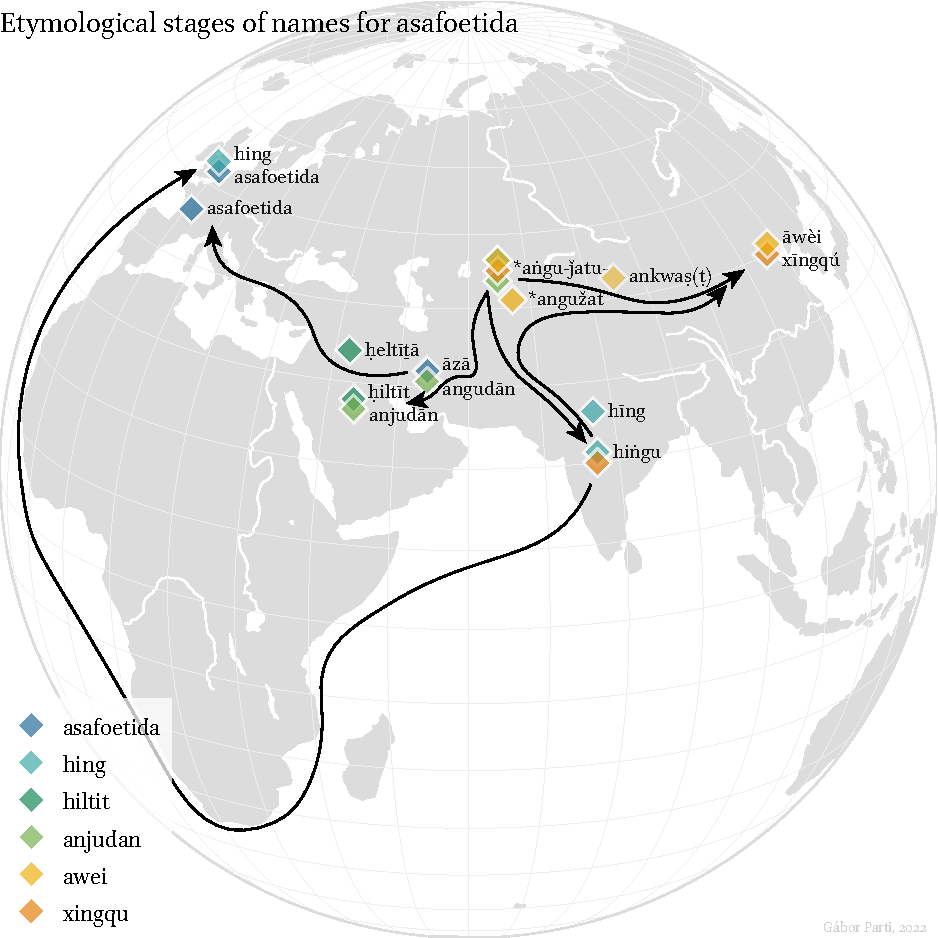
\includegraphics[width=\textwidth]{imgs/plots/diffusion_asafoetida_edited.pdf}
    \caption{Etymological stages in the progression of prototypical names of asafoetida.}
    \label{fig:cardamom_stages}
\end{figure}






% EE:
% asafoetida 
% resinous gum with a strong smell. XIV. — medL., lit. ‘stinking asa’, i.e. asa (usu. derived from a Persian azā mastic, but this word is of doubtful authenticity), fœtida, fem. of fœtidus FETID.

% OE:
% asafoetida (n.)
% alternative spelling of asafetida (q.v.); also see oe.
% asafetida (n.)
% "pungent sap from the roots of several plants native to Persia and Afghanistan," used as a drug, late 14c., from Medieval Latin asa (Latinized from Persian aza "mastic") + foetida, fem. of foetidus "stinking" (see fetid).

% MW:
% Middle English asafetida, from Medieval Latin asafoetida, from asa gum (of Iranian origin; akin to Persian azā mastic) + Latin foetida, feminine of foetidus fetid
% First Known Use: 14th century

% AH:
% [Middle English, from Medieval Latin asafētida : asa, gum (from Persian azā, mastic) + Latin foetida, feminine of foetidus, stinking; see FETID.]

% WK:
% Late Middle English, from Medieval Latin asafoetida, from Persian ازا / آزا (azâ, âzâ, “mastic”) + Latin foetida, feminine of foetidus (“bad-smelling”). 


% Synonyms: asant, hing, devil's dung

% MW:
% Hindi hī̃g, from Sanskrit hiṅgu

% AH:
% [Hindi, hīṁg, from Prakrit hiṁgu-, from Sanskrit hiṅgu, perhaps of Iranian origin; akin to Persian angu- in angužad, asafetida (angu- + žad, gum, tears of sap).]

% WK:
% From Hindi हींग (hīṅg). 





\clearpage \section{Black Pepper}
\label{sec:pepper}

\begin{spice}\label{spice:pepper}
\textsc{Pepper} \hfill \href{https://powo.science.kew.org/taxon/682369-1}{POWO} \\
\textbf{English:} \textit{pepper}; \textit{black pepper}. 
\textbf{Arabic:} {\arabicfont{فلفل}} \textit{filfil, fulful}. 
\textbf{Chinese:} {\tradchinesefont{胡椒}} \textit{hújiāo} [foreign-pepper]; 黑胡椒 \textit{hēihújiāo} [black-barbarian-pepper]. 
\textbf{Hungarian:} \textit{bors}; \textit{fekete bors} [black pepper].  \\
\noindent{\color{black}\rule[0.5ex]{\linewidth}{.5pt}}
\begin{tabular}{@{}p{0.25\linewidth}@{}p{0.75\linewidth}@{}}
Plant species: & \taxonn{Piper nigrum}{L.} \\
Family: & \textit{Piperaceae} \\
Plant part used: & fruit \\
Region of origin: & Malabar coast (South India) \\
Cultivated in: & Vietnam; Brazil; Indonesia; India; Sri Lanka; etc. \\
Color: & black; white; green \\
\end{tabular}
\end{spice}

% \begin{figure}[!ht]
% 	\vspace{-4ex}
% 	\centering
% 	\subfloat{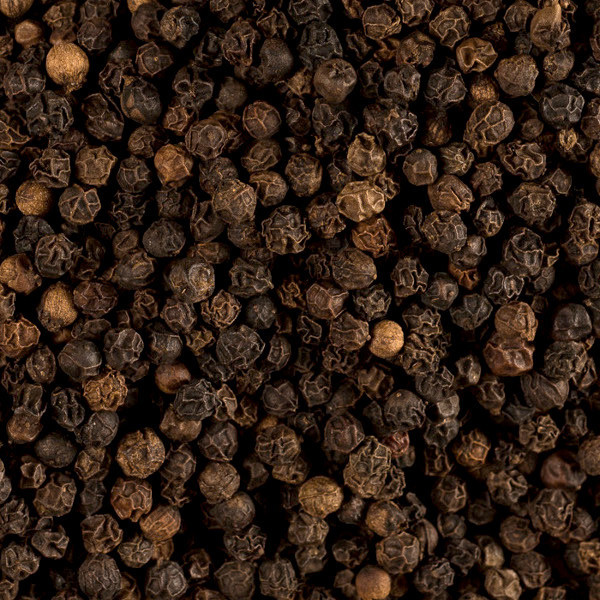
\includegraphics[width=0.3\linewidth]{imgs/spices/pepper-black-2.jpg}}
% 	\hfill
% 	\subfloat{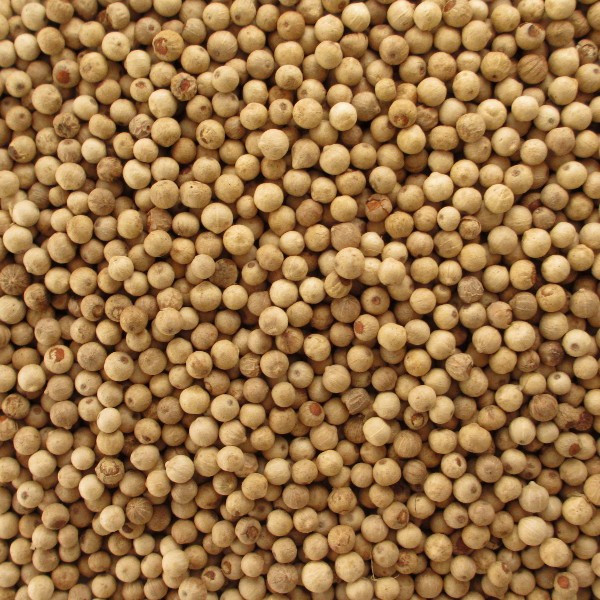
\includegraphics[width=0.3\linewidth]{imgs/spices/pepper-white-penja-2.jpg}}
% 	\hfill
% 	\subfloat{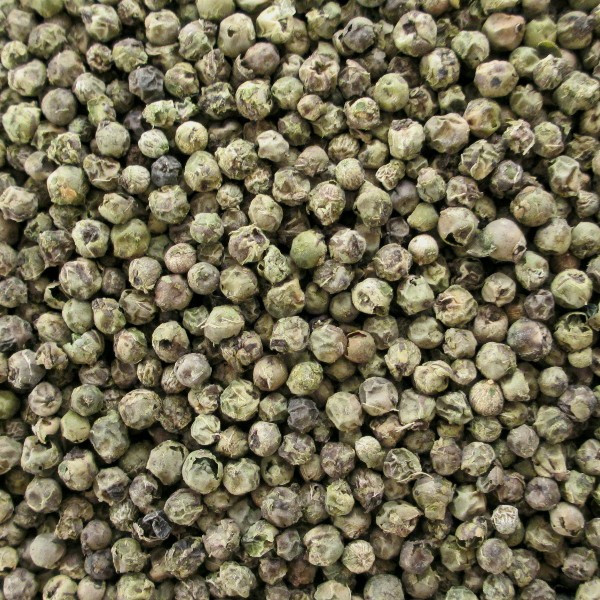
\includegraphics[width=0.3\linewidth]{imgs/spices/pepper-green-1.jpg}}
% 	\caption[Black, white, and green pepper.]{Black pepper from the Malabar coast in India, white pepper from the Penja Valley in Cameroon, and green peppercorns. \taxon{Piper nigrum}. Credits: Aromatiques.}
% 	\label{fig:pepper_imgs}
% \end{figure}

% DESCRIPTION:
Black pepper is the dried fruit (drupe)\footnote{Botanical term: A drupe refers to a type of fleshy fruit with thin skin and a single, central pit containing the seed, also known as a ``stone-fruit'' (e.g.: plum, cherry, peach, nutmeg, olive, mango). It is a term used to denote the contrast to a botanical ``berry'', which contains many seeds (e.g.: blueberry, grape).} of the species \taxon{Piper nigrum}. Pepper fruits are often called peppercorns, and they come in black, white, green, and even red. However, black pepper\index{pepper!black}, white pepper\index{pepper!white}, green\index{pepper!green} and ``true'' red peppercorns\index{pepper!red} are not different varieties, they are the fruits of the same plant. Their difference merely lies in the harvesting and drying process. All of them have a unique, pungent taste and a fresh, spicy aroma that they release when being crushed or ground. 

% INTRO:
Black pepper\index{pepper|textbf}\index{pepper!black} is the most important, most popular, and most consumed spice in the world \autocite[721]{mabberley_mabberleys_2017}. Valued for its pungency and flavor, pepper has been used since ancient times in traditional medicine and gastronomy from East to West, and it is the most influential spice that shaped human history. It is found and used virtually everywhere around the globe \autocite[253]{hill_contemporary_2004}, and most of us are familiar with the biting sensation it causes on the tongue and in the nose. Black pepper was one of the first aromatic substances used medicinally in India, and one of the first products of global commerce to be traded, alongside long pepper, and ginger. It was transplanted to other tropical regions of Asia early on, and cultivated extensively. Black pepper's early diffusion is remarkably interesting, it is the prototype spice for many of us. Also referred to simply as \textit{pepper} from here on, it was among the first oriental spices to reach the Occident \pvolcite[]{1}[86]{peter_handbook_2012}. Pepper was known to the ancient Egyptians, Greeks, and Romans in the West, and have changed medieval Europe. It was even used as currency in small amounts. Today it accounts for more than a third of all spices traded in the world, making it the most traded spice as well \autocite{ravindran_piper_2017}. Its importance is well demonstrated by the many books and monographs about its history \autocite[see][]{shaffer_pepper_2013,wernick_pepper_2014}, agronomy \autocite[see][]{ravindran_black_2000,nair_geography_2020}, and appeal \autocite[see][]{de_kerros_pepper_2016,barth_pepper_2019}.

% EXTRAS
Interestingly, black pepper is the only spice to be traded on the stock market as a commodity, the International Pepper Exchange was established in 1997 in Kochi, India. One result of this is cargo containers of black pepper sitting in warehouses waiting to change hands, leading to a loss in nutritional value and flavour and thus an unnecessary underwhelming experience for future consumers \autocite{madagascar_spices_company_madagascar_2022}. Spice merchants often urge serious customers to buy directly from the producer cutting the middlemen, citing the above inconvenience of product waiting in transit and retail.

\subsubsection{Uses}

% USES
% It was used
% for different purposes by different people in the past, and continue to be so currently and
% will remain so in future as well. For the civilized western people it is a spice, an essential
% additive to their food; for the ancient Egyptians it was an ingredient in the embalming
% mixture; for the ancient Aryans it was a valuable drug, and now for the common Indians
% pepper is a spice as well as a medicine, a sure cure for cold and fever and a component of
% many traditional Ayurvedic drugs. Stories richly coloured with imagination were carried
% by ancient sailors to distant places and its fame reached both Western and Eastern lands.
% The white pepper of commerce is also a product from the same pepper plant,
% produced by removing the pericarp (fruit wall) from ripe pepper fruits, which give the
% buff coloured seeds—the white pepper. White pepper is preferred in certain countries
% and also by the elite users because it gives a uniformly dull white powder; while black
% % pepper powder has the black component resulting from the powdered black pericarp.
% White pepper is traditionally prepared by steeping ripe fruits in water for a few days,
% rubbing to remove the pericarp; washing and drying. Indonesia is the major producer \autocite[1]{ravindran}

Black pepper had and has various uses in multiple areas. Nowadays, we mainly consider its importance in the culinary arts --- from seasoning food in the kitchen to the dining table --- but it is extensively used in the food industry as well for flavouring and preserving processed foods \pvolcite[]{1}[86]{peter_handbook_2012}.
% CULINARY USES:
Often called the ``king of spices'', black pepper is so ubiquitous and well known in cooking that it is essentially pointless to list cuisines and dishes that feature it. It is present in practically all savoury dishes, sauces, marinades, and pickles. It is used whole, crushed, or ground, and its role in Western gastronomy is well marked by the fact that virtually all restaurant table host a pair of salt and pepper mills or shakers. On the other hand, white pepper is a key ingredient in French and Chinese cuisine, where it is much more popular than black pepper, while green pepper is popular in Thai and South Indian cooking. 
% SEE PETER FOR MORE CULINARY
% MEDICINE
But besides just a seasoning, pepper also has roles in perfumery and beauty care, not to mention its use as a home remedy \autocite[467]{ravindran_black_2000}. In fact, as it is true for most spices, pepper in the past was considered primarily a medicine. Black pepper is well known in the traditional herbal systems, whether Ancient Greek, Ayurvedic, or Traditional Chinese Medicine, as well as contemporary pharmacology and phytotherapy (a modern name for chemistry-assisted herbalism). Reviews and updates on the research of \textit{Piper nigrum}, its active components, and their effects on human physiology are being published at a steady pace \autocite[see][]{srinivasan_black_2007, butt_black_2013, meghwal_piper_2013, haq_piperine_2021}. Recent scientific research shows that piperine displays numerous pharmacological effects, such as antimicrobial and antioxidant \autocite{haq_piperine_2021}. It is therefore not surprising that health benefits of black pepper have been recorded in pharmacopoeias since ancient times, and that it has been used for the treating of various illnesses: ranging from stomach pains and digestive problems to fever, cold, and even food poisoning \autocite[2952]{quattrocchi_crc_2014}.

% OPERATIVE
\begin{note}
Throughout this dissertation --- unless stated otherwise --- the term \textit{pepper} alone always denotes the pepper(s) of \taxon{Piper nigrum}, of the genus \textit{Piper}, from the pepper family (\taxon{Piperaceae}) or , originating in India (i.e. black pepper, white pepper, etc.). This is to make an arbitrary distinction with the various kinds of hot chile, or chili peppers of the genus \textit{Capsicum} in the nightshade family (\textit{Solanaceae}), native to the Americas. A partial objective of this dissertation is to untangle the messy nomenclature around these plant and spice names, which is evident if we take into account all the different items we can refer to with the words \textit{pepper} in English, \textit{jiāo} in Chinese, and \textit{filfil} in Arabic; a situation true to many other languages as well. 
% This notion is explored in more detail in \cref{sec:conundrum}
\end{note}

\subsubsection{False peppers}

There are other aromatic, spice yielding plants (other kinds of peppers, if you like) in the \textit{Piperaceae} family, constituting to different species, such as cubebs, tailed peppers, or Java peppers (\taxon{Piper cubeba}), (Indian) long peppers (\taxon{P. longum; P. retrofactum}), ``piper chilies'' (\taxon{P. chaba}), Ashanti/Benin pepper (\textit{P. guineense}), etc., and they will be referred to using these common names throughout. Cubeb, and  long pepper especially, were more common in ancient times but virtually disappeared from the global spice trade in the modern age. Other, less common spices unrelated to the \textit{Piper} genus, such as pink peppercorns from South America (\textit{Schinus molle; S. terebinthifolia}), Sichuan peppers from East Asia (\textit{Zanthoxylum spp.}), and alligator peppers (\taxon{Aframomum danielli}) from Africa are sometimes referred to as ``false peppers''. These will always be referred to with their usual full vernacular names to avoid confusion.
% (America pepper: chili) and peppercorn more to true pepper) explain in the pepper conundrum section.

Do other peppers at the end of this






\subsection{The Botany of Black Pepper} 

% ORIGIN:
Pepper is native to the Malabar region in South India where the Western Ghats, a mountain range parallel to the coastline, traps the monsoon rains. This results in the most humid region in India, making it one of the plant biodiversity hot-spots on Earth \autocite[1]{ravindran_black_2000}. Often called the ``king of spices'', pepper originates here in the evergreen tropical forests of Kerala, which is the origin and centre of plant diversity for the ``queen of spices'' as well: cardamom \autocite[1]{ravindran_black_2000}.
Wild populations of pepper and closely related species grow in the moist, shady forests, up to 1200\,m above sea level \autocite{ravindran_piper_2017}. Pepper is cultivated for thousands of years in these areas, and once South India was the only place that produced it. Due to the human desire for this valuable spice, the crop was slowly transplanted from here to other tropical zones, mainly in the Asia-Pacific: Sri Lanka, Malaysia, Indonesia; but also to the West as far as Madagascar and Brazil. Today it is cultivated in 26 countries \autocite{ravindran_black_2000}. The top five producers in 2020 were Vietnam, Brazil, Indonesia, India, and Sri Lanka.\footnote{In order of production quantity, from highest to lowest. All production data is from FAOSTAT (Food and agriculture data of the Statistics Division, Food and Agriculture Organization of the United Nations): \url{https://www.fao.org/faostat/en/\#home}; license: CC BY-NC-SA 3.0 IGO.}
% THE PLANT:
Pepper grows on a perennial vine, blooming a cluster of small flowers on hanging spikes that bring young, round fruits that are first green, turning to bright red as they ripen; resembling berries. Pepper plants in their native habitats spread on the forest floor, or climb over rocks, shrubs, and trees. Pepper prefers the hot tropics with high humidity, and optimal temperatures of around 20-30°C. Open cultivation is possible in places where rainfall is well distributed (e.g.: Thailand, Vietnam, Malaysia), whereas in India shade is required because of the 6 months of drought between monsoon seasons \autocite{ravindran_piper_2017}. Wild pepper species are dioecious\footnote{Bot.: the male and female reproductive organs are found in separate individuals.}, having male and female individuals, while the domesticated pepper populations became monoecious:\footnote{Bot.: having both the male and female reproductive organs in the same individual; hermaphrodite.} one plant is both male and female. This is probably due to thousands of years of selective multiplication and it leads to greater quantities in production: bisexual flowers mean high fruit yields \autocite[38]{ravindran_black_2000}.
% CULTIVATION:
Pepper lianes are propagated from cuttings, and being climbers, they are usually grown around trees for live support, or with the use artificial poles \autocite[216]{van_wyk_culinary_2014}. 

% HARVESTING:
When it comes to harvesting, the techniques are different depending on the intended end product. In the case of black pepper, the near-ripe (still green) fruits are hand-picked and sun-dried in the course of several days up to two weeks. Oxidization leads to the darkening of the pericarp\footnote{Bot.: In fruit anatomy, pericarp is the collective name for the outer layers around the seed of a fleshy fruit or drupe: the endocarp (innermost covering of the seed; the pit), the mesocarp (flesh), and the exocarp (skin).} (the outside skin and flesh of the fruit) to a hue ranging from deep brown to jet black, while also attaining the signature wrinkles and dimples \autocite[254]{hill_contemporary_2004}. The drying process can be sped up by boiling the pepper fruits in hot water for a short time. Chemical changes induced by the heat hasten the subsequent oxidization process, which causes the outer layer to gradually shrivel and blacken while getting dried \autocite[216]{van_wyk_culinary_2014}. White pepper is obtained by letting moisture and micro-organism dissolve the cellular tissue of the fully ripe red fruits, basically letting them rot in a technique called retting\footnote{}. The fruits' decomposed skin and flesh are easily removed by hand or machine after soaking and gentle washing, and the remaining pale seed is then dried on the sun, or bleached \autocite[216]{van_wyk_culinary_2014}. Green peppercorns are a result of traditional pickling, or in modern times rapid freeze-drying of the unripe fruits as a way to prevent fermentation. This process results in a product with a light weight and seemingly higher price. Occasionally the ripe, red fruits are sold as well to be used fresh, but the ``true'' red peppercorns -- as \textcite{hill_contemporary_2004} calls them -- are rare and mostly found in producing areas: they loose their vigour within days of harvest and so must be used fresh unless preserved in vinegar or brine. As it is a hallmark of spices, the two varieties that are dried (black pepper and white pepper) are much more known worldwide, their dry quality allows them to be transported on longer journeys. If we think of white pepper as de facto decorticated black pepper, we would rightly guess that the flavour of white pepper is weaker than black pepper, as the outer peel of black pepper contains much of the spicy compounds responsible for the heat. Green peppercorns have an even milder taste and a much shorter shelf-life.
%CULTIVARS
Indigenous to the Malabar coast, a well known and popular variant is the Malabar pepper or Malabar black, a commodity sought-after by traders since Roman times \autocite{de_romanis_indo-roman_2020}. Another famous name on the market is the Tellicherry black, which according to spice traders is not a regional designation, but rather a requirement of size. If a peppercorn is larger than 4.25 mm pinhead, it is classified as Tellicherry \autocite{eirinberg_tellicherry_2021}. Other famous and/or protected pepper variants with Geographical Indication (GI) certificates are Kampot pepper from Cambodia, the Muntok white and Sarawak white from Indonesia and Malaysia respectively, and the Penja pepper from Cameroon. A relatively recent publication by pepper grower and merchant \textcite{de_kerros_pepper_2016} accompanied by remarkable photographs aims to present all the dozens of pepper varieties around the world that are available to those with an adventurous taste.
% FLAVOUR COMPOUNDS:
Pepper owes its punch to the alkaloid piperine, while the wrinkly pericarp supplies the complex spicy aroma and flavour thanks to a high number of chemical compounds in the form of volatile oils \autocite[467]{ravindran_black_2000}. The most powerful one of which is rotundone, a highly potent compound also found in Shiraz wines \autocite{wood_wine_2008}. For more on details on the botany, chemistry, cultivation, agronomy, and other aspects of black pepper, please refer to \textcite{ravindran_black_2000, nair_agronomy_2011, parthasarathy_chemistry_2008}.



% HISTORY:
\subsection{The History of Black Pepper}

The history of pepper accompanies the history of mankind from the earliest times of contact and exchange between civilizations. The story of pepper is global and must travel to Ancient Egypt to begin. According to a popular anecdote in books and articles about pepper, peppercorns were used in the embalming process of mummies \autocite{ravindran_black_2000}, and they were found in the nostrils of Ramses II \autocite[168]{turner_spice_2004}. I have read this on many occasions, and I have spend way too much time to find out if this is true or not. In short, I there is no definitive answer, but that the alleged peppercorns were only ``seen'' through X-ray, and that the original reports are dubious at best, as reported by \textcite[206]{bucaille_mummies_1990}. Ramses II died in 1213 \BC{}, and even if these specific are problematic, it is said that peppercorns and cinnamon were imported ``from Southeast Asia and the East Indies'' and thus available to wealthy citizens of Egypt as early as New Kingdom era (\nth{16} c. \BC{}--\nth{11} c. \BC{}) \autocite[394]{salima_diet_2005}.

Pāṇini, the famous Sanskrit grammarian (ca. 4--\nth{6} c. \BC{}) recorded the use of pepper in spiced wine, and pepper appears in early Indian medical texts of Suśruta as well \autocite{ravindran_black_2000}. In the \nth{4} century, Theophrastus recorded and described both black pepper and long pepper, and by the \nth{1} century \AD{} its source was accurately describe by Pliny the Elder; stating that black pepper is from south, long pepper is from north India. Rome conquered Egypt in 30 \BC{}, and with that the pepper trade as well, which was a key enterprise in Rome's later financial success. From here onwards, the history of pepper within the Indo-Roman trade is well studied and documented, for further details please see \textcite{sidebotham_berenike_2011,de_romanis_indo-roman_2020,miller_spice_1969}. 

% Peppercorn in fist century as far as Germany (Czarra)

During the late Middle Ages, pepper also brought great riches to Europe, the former wealth of Venice was due to its trade. After the crusades, European sea powers tried to get ahold on the monopoly of the spice trade, and Vasco de Gama's landing near Calicut in 1498 in the Venetian, Portuguese, Spanish, Dutch, and English vied with each other for centuries up to the modern era. Pepper reached Southeast Asia probably during the t The story of pepper is very well explored in the Age of Exploration as well, there is no need for me to delve into it deeper. I recommend \textcite{shaffer_pepper_2013,turner_spice_2004,dalby_dangerous_2000} for those interested.

% A Chinese envoy visited the Malabar coast in search of pepper. 4th c. BC? Who

% TIMELINE IN RAVINDRAN
% Originally black pepper was a forest produce
% Black pepper was essentially a forest produce in the past, people collected it from
% forests, where it abounded. The collected pepper was brought to local markets for
% retail trade with Arab merchants. Domestication of pepper appears to be a much later
% event. There is, only speculative evidence as to when pepper was introduced to other
% countries as a domesticated crop. Colonists from India are believed to have introduced
% pepper cultivation to Indonesia about 100 B.C. (Rosengarten 1973). Many such
% introductions surely might have taken place subsequently also. The landmarks in the
% colourful history of pepper are given below. Ravindran 2000 

% \autocite{pegolotti_pratica_1936}

% Wyk:
% Pepper featured prominently in the
% ancient world and was a source of fabulous wealth
% during the medieval and colonial spice trade. The
% Dutch and Afrikaans expression “peperduur”
% reflects the high price it once had. Pepper provided
% the pungency (“pep”) of Indian food until it was
% partially replaced by chilli peppers from the New
% World. It nevertheless remains the most important
% and popular of all spices in terms of overall value
% and trade volume.

% Black pepper is the most important and widely used spice. Black pepper (hereafter mentioned simply as pepper) is valued for its characteristic pungency and flavour. It has been used extensively from ancient times as a spice and condiment in a variety of food preparations. Pepper is famous as a traditional medicine; it is also famous as a home remedy. Globally, pepper accounts for 34\% of the total spices traded. In all countries pepper is used for flavouring food and for preserving processed foods. Pepper played a very significant role in shaping the history of mankind. It was the first oriental spice to reach the Western world. The European nations vied with each other to get the monopoly over the spice trade and hegemony over the spice-producing countries of the East that eventually led to the discovery of a sea route to India by Vasco da Gama. This event changed the history of the world radically in the centuries that followed. ENCYC

% Among the spices, black pepper is the king. It is the most important, the most
% popular and the most widely used spice in the world. It has extensive culinary uses
% for flavoring and preserving processed foods and is also important medicinally. Of
% the total spices traded internationally, pepper accounts for about 34 % (throughout
% this chapter, pepper is used to mean black pepper, unless otherwise stated). South
% West India, particularly the Western Ghats regions of the South India, is the centre
% of origin of this important spice. Black pepper was the fi rst oriental spice to be
% introduced into the Western world, and it was well known among the Romans and
% Greeks. In the Middle Ages, pepper, assumed great importance in Europe. Its use
% resulted in revolutionary changes in western cooking. For a comprehensive treatment
% of black pepper, the reader may consult Ravindran (2000a) and Ravindran
% et al. (2006). Bezerra et al. recently (2009) summarized the various aspects of black

\subsection{The Names of Black Pepper}

\subsubsection{English}

\begin{etymology}\label{ety:pepper}
English \textit{pepper}
<\textss{?} West Germanic* \textit{*pipor} `id.'
< Latin \textit{piper} `black pepper, long pepper'
< Ancient Greek {πέπερι} \textit{péperi} `id.'
< Middle Indo-Aryan* {पिप्परी } \textit{pipparī} `long pepper'
< Sanskrit {पिप्पलि } \textit{pippali} `long pepper \textit{Piper longum} (plant and berry); a berry'\footnote{\textcite{oed; med; bosworth_anglo-saxon_2014}; \textcite{oe}; \textcite{lewis_latin_1879}; \textcite{liddell_greek-english_1940}; \textcite[599]{sheth_paia-sadda-mahannavo_1923}; \textcite[626]{monier-williams_sanskrit-english_1899}}
\end{etymology}

The word \textit{pepper} arrived to modern English via Middle English \textit{peper} and Old English \textit{pipor, piper}, from an early, Proto-West Germanic borrowing of Latin \textit{piper}.\footcite[pepper]{oed} The Latin word comes from Greek \gr{πέπερι} \textit{péperi}, a word ``of oriental origin''\footcite[pepper]{hoad_concise_2003} or ``Indic origin''.\footcite[pepper]{ahd} The source is most probably from a Middle Indo-Aryan language, akin to Prakrit \textit{pipparī}\footcite[599]{sheth_paia-sadda-mahannavo_1923}, probably via Pahlavi (Middle Persian)\footcite[pepper]{oe}, ultimately from Sanskrit \textit{pippali} or \textit{pippalī}.\footcite[628 \link{https://www.sanskrit-lexicon.uni-koeln.de/scans/MWScan/2014/web/webtc/servepdf.php?page=0628}]{monier-williams_sanskrit-english_1899}

As for the meaning, we know that in Latin the word \textit{piper} was used for both black pepper and long pepper, and this is true for the Greek word as well. As long pepper gradually disappeared and was completely replaced by black pepper in the Middle Ages, so vaned the that sense of the word. The original word's meaning however was exclusively long pepper, \textit{pippali} did not refer to black pepper. In \textcite{monier-williams_sanskrit-english_1899}, \textit{pippali} is `long pepper', while \textit{pippalī} refers to `a berry; Piper longum (both plant and berry)'. The Sanskrit word for `black pepper' was \sa{मरिच} \textit{marica}\footcite[790]{monier-williams_sanskrit-english_1899}, attested in the \gls{Sushruta}, the foundational text of \gls{Ayurveda}. Hindi-Urdu \sa{मिर्च}/\fa{مرچ} \textit{mirch} is the most obvious descendant of the Sanskrit word, and it is similar in meanings to the word \textit{pepper} in English today: by itself it rather refers to chili, while with a distinguishing word, it refers to black pepper (i.e. \textit{kālī mirc} [black pepper]). The use of both black and long pepper in India can be dated to ancient times, as Ayurvedic texts compiled in Sanskrit, such as the \gls{Sushruta} testify. Together with ginger (\textit{śṛṅgavera} in Sanskrit), these three spices are a base combination in traditional Indian medicine, the name for which is \sa{त्रिकटु} \textit{trikaṭu} `three spices'.

The ancestors of English speakers adopted the word during the Anglo-Saxon period, before they arrived to England, and so its cognates are found in other West Germanic languages as well.\footcite[pepper]{cresswell_oxford_2021} 

% Cognates:  Old Saxon \textit{pipari}, \textit{pepar} (Dutch \textit{peper}, Scots pepar), Old High German \textit{pfeffar} (German \textit{Pfeffer}), Old Norse \textit{piparr} (Danish \textit{peber}, Swedish \textit{peppar}, Icelandic \textit{pipar}).

According to \textcite[695]{mabberley_mabberleys_2017}, the following common names refer to the species \textit{Piper nigrum}: pepper, black pepper, Madagascar pepper, and white pepper. Except the green peppercorns mentioned above, other spices, such as the Sichuan peppers from China, pink peppercorns from Brazil, and Guinea peppers (\textit{Aframomum melegueta}) from tropical West Africa are different, often botanically unrelated species. Only connected by their names and similar uses, looks, or flavour profiles.


% Leaves of P. sarmentosum are the cha plu of Thai cuisine and those of P. auritum the hoja santa of Mexican cuisine. Plus Piper betle = betel? no.

% \begin{table}[!ht]
\centering
\begin{tabularx}{\textwidth}{@{}l>{\itshape \small}lL>{\small}l@{}}
\toprule
\textbf{\#} & \multicolumn{1}{l}{\textbf{Species}} & \multicolumn{1}{l}{\textbf{Name}} & \multicolumn{1}{l}{\textbf{Source}} \\
\midrule
1	& Piper nigrum	& black pepper	& \textcite{van_wyk_culinary_2014} \\
2	& Piper nigrum	& green pepper	& \textcite{oed} \\
\textbf{3}	& \textbf{Piper nigrum}	& \textbf{pepper}	& \textbf{\textcite{van_wyk_culinary_2014}} \\
4	& Piper nigrum	& peppercorn	& \textcite{oed} \\
5	& Piper nigrum	& white pepper	& \textcite{oed} \\
\bottomrule
\end{tabularx}
\caption{Various names for pepper in English.}
\label{table:names_pepper_en}
\end{table}



% \subsubsection{Arabic}

% \begin{etymology}\label{ety:fulful}
Arabic {فلفل} \textit{filfil, fulful} `pepper'
< Persian {پلپل} \textit{pilpil} `id.'; cf. cognates Old Armenian \hy{պղպեղ} \textit{płpeł}, Old Georgian \ka{პილპილი} \textit{ṗilṗili}
<\textss{?} Middle Indo-Aryan \textit{?} `long pepper'
< Sanskrit {पिप्पलि } \textit{pippali} `long pepper \textit{Piper longum} (plant and berry); a berry'\footnote{\textcite[2434]{lane_arabic-english_1863}; \textcite{sq}}
\end{etymology}

% \begin{table}[!ht]
\centering
\begin{tabularx}{\textwidth}{@{}l>{\itshape \small}lr>{\itshape}lL>{\small}l@{}}
\toprule
\textbf{\#} & \multicolumn{1}{l}{\textbf{Species}} & \multicolumn{1}{l}{\textbf{Name}} & \multicolumn{1}{l}{\textbf{Tr.}} & \multicolumn{1}{l}{\textbf{Gloss}} & \multicolumn{1}{l}{\textbf{Source}} \\
\midrule
\textbf{1}	& \textbf{Piper nigrum}	& \textbf{فلفل}	& \textbf{fulful}	& \textbf{pepper}	& \textbf{\textcite{wehr_dictionary_1976}} \\
2	& Piper nigrum	& فلفل أبيض	& fulful abyaḍ	& white pepper	& \textcite{baalbaki_-mawrid_1995} \\
3	& Piper nigrum	& فلفل أسود	& fulful aswad	& black pepper	& \textcite{baalbaki_-mawrid_1995} \\
4	& Piper nigrum	& فلفلة	& fulfula	& peppercorn	& \textcite{wehr_dictionary_1976} \\
\bottomrule
\end{tabularx}
\caption{Various names for pepper in Arabic.}
\label{table:names_pepper_ar}
\end{table}



% \subsubsection{Chinese}

% \begin{etymology}\label{ety:hujiao}
\textbf{Mandarin Chinese} {胡椒} \textit{hú​jiāo} `black pepper' [barbarian-pepper], from 胡 \textit{hú​} `Western barbarians, steppe nomads' + 椒 \textit{jiāo} `pepper, spice' (\textit{jiāo} was the prototype spice in China, originally referring to the local ``Sichuan pepper'' which is now called 花椒 \textit{huājiāo} [flower-pepper]), [Northern and Southern] 420-445\footnote{\textcite{schuessler_abc_2007}}
\end{etymology}

% \begin{table}[!ht]
\centering
\begin{tabularx}{\textwidth}{@{}l>{\itshape \small}ll>{\itshape}lL>{\small}l@{}}
\toprule
\textbf{\#} & \multicolumn{1}{l}{\textbf{Species}} & \multicolumn{1}{l}{\textbf{Name}} & \multicolumn{1}{l}{\textbf{Tr.}} & \multicolumn{1}{l}{\textbf{Gloss}} & \multicolumn{1}{l}{\textbf{Source}} \\
\midrule
1	& Piper nigrum	& \tradchinesefont{白胡椒}	& báihújiāo	& white-barbarian-pepper	& \textcite{mdbg} \\
\textbf{2}	& \textbf{Piper nigrum}	& \textbf{\tradchinesefont{胡椒}}	& \textbf{hújiāo}	& \textbf{barbarian-pepper}	& \textbf{\textcite{hu_food_2005}} \\
3	& Piper nigrum	& \tradchinesefont{黑胡椒}	& hēihújiāo	& black-barbarian-pepper	& \textcite{mdbg} \\
4	& Piper nigrum	& \tradchinesefont{綠胡椒}	& lǜhújiāo	& green-barbarian-pepper	& \textcite{regency_spices_regency_2022} \\
5	& Piper nigrum	& \tradchinesefont{青胡椒}	& qīnghújiāo	& green-barbarian-pepper	& \textcite{regency_spices_regency_2022} \\
\bottomrule
\end{tabularx}
\caption{Various names for pepper in Chinese.}
\label{table:names_pepper_zh}
\end{table}



% \subsubsection{Summary}

% \begin{table}[!ht]
\centering
\begin{tabularx}{\textwidth}{@{}ll>{\itshape}lLl>{\small}l@{}}
\toprule
\textbf{\#} & \textbf{Language} & \multicolumn{1}{l}{\textbf{Term}} & \textbf{Gloss} & \textbf{Loan} & \multicolumn{1}{l}{\textbf{Source}} \\
\midrule
1	& English	& black pepper	& 	& maybe	& \textcite{oed} \\
2	& English	& pepper	& 	& yes	& \textcite{oed} \\
3	& English	& white pepper	& 	& maybe	& \textcite{oed} \\
\midrule
1	& Arabic	& fulful	& pepper	& yes	& \textcite{wehr_dictionary_1976} \\
2	& Arabic	& fulful abyaḍ	& white pepper	& no	& \textcite{baalbaki_-mawrid_1995} \\
3	& Arabic	& fulful aswad	& black pepper	& no	& \textcite{baalbaki_-mawrid_1995} \\
4	& Arabic	& fulfula	& peppercorn	& no	& \textcite{wehr_dictionary_1976} \\
\midrule
1	& Chinese	& báihújiāo	& white-barbarian-pepper	& no	& \textcite{mdbg} \\
2	& Chinese	& hújiāo	& barbarian-pepper	& no	& \textcite{defrancis_abc_2003} \\
3	& Chinese	& hēihújiāo	& black-barbarian-pepper	& no	& \textcite{mdbg} \\
\bottomrule
\end{tabularx}
\caption{Conventionalized names for pepper in English, Arabic, and Chinese, found in dictionaries.}
\label{table:names_pepper}
\end{table}










% \begin{figure}[!hbt]
%     \centering
%     \includegraphics[width=\linewidth]{imgs/pepper.pdf}
%     \caption{Etymology of the English word \textit{pepper}, and an illustration of its approximate route.}
%     \label{map:pepper_etymology}
% \end{figure}



% EE: The Concise Oxford Dictionary of English Etymology:
% OE. piper, -or = OS. pipari, pepar (Du. peper), OHG. pfeffar (G. pfeffer); WGmc. — L. piper — Gr. péperi, of oriental orig.; cf. Skr. pippalī́t berry, peppercorn.

% OE: 
% pepper (n.)
% "dried berries of the pepper plant," Middle English peper, from Old English pipor, from an early West Germanic borrowing of Latin piper "pepper," from Greek piperi, probably (via Persian) from Middle Indic pippari, from Sanskrit pippali "long pepper." The Latin word is the source of German Pfeffer, Italian pepe, French poivre, Old Church Slavonic pipru, Lithuanian pipiras, Old Irish piobhar, Welsh pybyr, etc.
% Application to fruits of the Capsicum family (unrelated, originally native of tropical America) is from 16c. To have pepper in the nose in Middle English was "to be supercilious or unapproachable."
% pepper (v.)
% "to sprinkle as with pepper," 1610s, from pepper (n.). Old English had gepipera. Meaning "to pelt with shot, etc.; hit with what pains or annoys" is from 1640s. Related: Peppered; peppering.

% MW:
% Middle English peper, from Old English pipor; akin to Old High German pfeffar pepper, Old Norse piparr; all from a prehistoric Germanic word borrowed from Latin piper pepper, from Greek peperi, probably from Sanskrit pippali long pepper
% First Known Use: before 12th century (sense 1a)

% AH:
% [Middle English peper, from Old English pipor, from Latin piper, long pepper, black pepper, from Greek peperi, of Indic origin; akin to Prakrit pipparī, long pepper, from Sanskrit pippalī, from pippalam, berry, fruit of the pipal tree, of unknown origin.]

% WK:
% From Middle English peper, piper, from Old English piper, from Proto-West Germanic *piper, from Latin piper, from an Indo-Aryan source; compare Sanskrit पिप्पलि (pippali, “long pepper”). The name was given to the capsicum fruit because of its unusual spicy taste, not unlike the European spice.

% Wo: The Oxford Dictionary of Word Origins:
% The Anglo-Saxons adopted the word for this highly prized spice before they invaded England, for it is found in other West Germanic languages. The word came via Latin from Greek peperi, from Sanskrit pippalī ‘berry, peppercorn’. 
%The phrase peppercorn rent is from the once-common practice of stipulating the payment of a peppercorn as a nominal rent. (true?)
% Cognate with Scots pepar, Saterland Frisian Pieper, West Frisian piper, Dutch peper, German Low German Peper, German Pfeffer, Danish peber, Swedish peppar, Icelandic pipar. Doublet of peepul. 



% The pepper conundrum:

% Before we delve into the chaos of \textit{pepper-linguistics}, we should make the botany and geography absolutely clear. There are essentially three major sources of edibles we can refer to as peppers: (1) \textit{Piper}, a pantropical\footnote{??} genus known for black and white pepper, long pepper, and cubeb pepper from South and South East Asia; (2) \textit{Capsicum}, the genus of both hot chile and mild bell pepper species and their numerous cultivars native to the Americas; and (3) \textit{Zanthoxylum}, a vast and cosmopolitan\footnote{??} genus of various species yielding Sichuan peppers favoured in East Asia. There are many more aromatic products denoted with the name \textit{pepper} in English, but for our task focusing on the above three genera is sufficient. Also, the majority of globally relevant ``peppers'' belong to these groups as well. Nevertheless, for a full paragraph of a detailed list of plants, please see \textcite[695]{mabberley_mabberleys_2017}.

% pepper Piper nigrum; African p. Xylopia aethiopica; Ashanti or Benin p. P. guineense; bell p. Capsicum annuum Grossum Group; p.berry Drimys spp.; betel p. P. betle; bird p. C. a.var.glabriusculum; black p. P. nigrum; bush p. Clethra alnifolia; cayenne p. Capsicum annuum Longum Group; cherry p. C. a. Cerasiforme Group; chilli p. C. a.Longum Group; Chinese p. Zanthoxylum simulans; cone p. C. a. Conoides Group; p.corns, pink or red Schinus terebinthifolius; Ethiopian p. X. aethiopica; green p. C. a. Grossum Group; Guinea p. Aframomum melegueta, X. aethiopica; Indian long p. P. longum; Jamaican p. Pimenta dioica; Japanese p. Z. piperitum; Java p. Piper cubeba; Kawa p. P. methysticum; long p. P. longum; Madagascar p. P. nigrum; malagueta or melegueta p. A. melegueta; negro p. X. aethiopica; red or sweet p. C. a. Grossum Group; Saturday-night p. Euphorbia helioscopia; Sichuan p. Z. simulans; p. tree S. molle, Kirkia wilmsii, P. excelsum; wall p. Sedum acre; water p. Persicaria hydropiper; W African black p. Piper clusii; white p. P. nigrum

% Pepper in English

% ...


The confusion of the two kinds of pepper -- most notably of black pepper and chile pepper in English -- is also present in Chinese, as well Arabic. Whether in culinary or medicinal spice terminology, or just in vernacular names in daily conversation, the curse of ``one word for all peppers'' is present in many languages.

\textit{Jiao} `pepper' in Chinese

In Chinese, the word for `pepper' is \textit{jiao}. And just like in English, \textit{jiao} now can refer to all the three major sources of pepper. So which pepper is it? \st{Who is the O.G. of peppers?}. It would be safe to assume that \textit{jiao} originally referred to indigenous Chinese peppers of various \textit{Zanthoxylum} species, or Sichuan peppers as we today call them. We can find instances of Classical Chinese texts featuring the pepper plant, \textit{jiao} and it's branches appear in a poem from the \textit{Book of Poetry}:

% \poemtitle{Mathematics}
\settowidth{\versewidth}{The clusters of the pepper plant,}
\begin{verse}[\versewidth]
椒聊之實、蕃衍盈升。\\
彼其之子、碩大無朋。\\
椒聊且、~~~~~~遠條且。\\!
The clusters of the pepper plant,\\
Large and luxuriant, would fill a pint.\\
That hero there\\
Is large and peerless.\\
O the pepper plant!\\
How its shoots extend!\\
\end{verse}
\attrib{Translated by James Legge, \\
from the \textit{Shijing}, \\
c. 8--\nth{11} century \BC.}

% Pre-Qin and Han -> Ancient Classics -> Book of Poetry -> Lessons from the states -> Odes Of Tang -> Jiao Liao

% Transl. James Legge
% https://ctext.org/book-of-poetry/jiao-liao?searchu=%E6%A4%92%E8%81%8A%E4%B9%8B%E5%AF%A6%E3%80%81%E8%95%83%E8%A1%8D%E7%9B%88%E5%8D%87%E3%80%82&searchmode=showall#result
% \url{https://en.wikipedia.org/wiki/Classic_of_Poetry}

% Our assumption will only strengthen if we search the word history of black pepper, a native of India. It first appears in
% https://ctext.org/pre-qin-and-han?searchu=%E8%83%A1%E6%A4%92

% Pre-Qin and Han


% The first occurrence of \textit{hujiao}

% The origin of hujiao `black pepper' in Chinese






% \begin{figure}
% \label{fig:pepper}
% \begin{forest}
% for tree={grow'=0,calign=center,font=\footnotesize, s sep=1,inner sep=1,outer sep=1},
% forked edges,
% [Sanskrit\\pippali
%     [Ardhamagadhi Prakrit\\pipparī [Awadhi\\pīpri]]
%     [Gandhari [Middle Iranian\\\textrightarrow [Persian\\pelpel [Arabic\\\textrightarrow filfil [Persian\\\textrightarrow felfel]] [(Arabic)\\\textrightarrow falāfil] [Baluchi\\\textrightarrow pilpil] [Hebrew\\\textrightarrow pilpel] [Swahili\\\textrightarrow pilipili] ] [Old Armenian\\\textrightarrow płpeł [Armenian\\\textrightarrow płpeł]] [Old Georgian\\\textrightarrow ṗilṗili [Georgian\\ṗilṗili]] ]]
%     [Pali\\pipphalī]
%     [Magadhi Prakrit [Assamese\\pipoli] [Bengali\\pipul] [Bhojpuri\\pīpri]]
%     [Maharastri Prakrit [Old Marathi\\piṃpaḷī [Marathi\\pimpḷī]] [Kannada\\\textrightarrow hippali]]
%     [Sauraseni\\Prakrit [Nepali\\piplā] [Gujarati\\pīpar] [Hindustani [Hindi\\pīpal; pīpar] [Urdu\\pīpal] [(English)\\\textrightarrow peepul]] [Punjabi\\pippalī] [Ancient Greek\\\textrightarrow péperi* [Greek\\pipéri [Ottoman\\Turkish\\biber [Turkish\\biber [Armenian\\bibar] [Azerbaijani\\bibər] [Crimean Tatar\\biber] [Macedonian\\biber] [Serbo-Croatian\\biber]]] [Aromanian\\piper]] [Latin\\\textrightarrow piper [Basque\\\textrightarrow piperra] [Middle Irish\\pipur [Irish\\piobar] [Manx\\pibbyr] [Scottish Gaelic\\peabar; piobar] [Old Norse\\piparr [Icelandic\\pipar] [Faroese\\pipar] [Norwegian\\pepar] [Swedish\\peparr [Finnish\\\textrightarrow pippuri [Northern Saami\\bihppor]]]] ] [Dalmatian\\pepro] [Italian\\pepe] [Old French\\poivre [French\\poivre]] [Aragonese;\\Catalan;\\Occitan\\pebre]]]]
%     [Old Tamil\\\textrightarrow [Tamil\\tippili] [Malayalam\\\textrightarrow tippali]]
%     [Telugu\\\textrightarrow pippali]
%     [Thai\\\textrightarrow dii-bplii]
%     [Tibetan\\\textrightarrow pi pi ling]
%     [Middle Chinese\\\textrightarrow MC piɪt̚ bʉɐt̚ [Chinese\\bìbá [Japanese\\\textrightarrow hihatsu] [Korean\\\textrightarrow pilbal]]]
% ]
% \end{forest}
% \caption{Caption}
% \end{figure}





% \small{aguttam, akuttam, alar, alarkay, alarkaycceti, alarmancal,
% alivaliyanmani, amiram, anam, apanam, apayam,
% aricam, aricu, aricuvai, arisu, arittam, arunapakam, arutam,
% aruttakam, aruttam, aruttan, arutti, atittam, aucatikam,
% autatalakamilaku, ayilakikam, bikran, cakankam,
% canucam, canucam, canukam, carapantam, carumapantam,
% catalam, catalamilaku, cattu-molagoi, cavi, cavviyam, cavviyapalam,
% cavyam, celavikacceti, celaviyam, cevviyam,
% ceytakar, chocamirch, cirovikam, ciroviruttam, citamaricam,
% citamarucam, citamarucu, citamarukam, cullituvan,
% cunam, cuppiramaniyam, cur, dhanwantari, dharmapattana,
% dharmavarttana, dolo maricho, eddemunchi, eddemunci,
% fiffile-asvad, fifile-asvad, fifile-gird, filfil aswad, filfil-esiyah,
% filfil siah, filfile-gird, filfile-siyah, filfilgird, filful
% aswad, filfilsiya, filfiluswud, gol mirc, gol-mirch, golmirch,
% golmorich, gulmirch, habush, hapusha, impikam, impilam,
% irambivam, irampikam, irampilam, irampivam, itukam, itukamilaku,
% ivainakitam, ivanattam, jalook, jaluk, kaalimirch,
% kaalu menasu, kadu menasu, kali mirch, kalimirc, kalimirch,
% kalamiri, kalappakacceti, kalappakam, kali mirch, kalimirch,
% kalimirich, kalinai, kalinaikkollu, kalinaimilaku, kalinkam,
% kallinai, kami, kamicakam, kanakam, kanattai, kandanaguli,
% kankola, kantanakuli, kantankuli, kaphavirodhi,
% karam, karee menasu, kari, karikkay, karimenasu, karunelli,
% karutturupayan, karyam, katti, kattirican, katu, katuka, kay,
% kayam, kevakatiraviyam, kevalatiraviyam, kirantikantikam,
% kirusnam, kiruttinam, kola, kolai, kolagam, kolaka, kolakam,
% kolam, kolicam, kolikacceti, krishnam, krishnamushana,
% krsna, kuru-milagu, kuru-mulaka, kurumilagu, kurumilaku,
% kurumulagu, kurumulaka, kurumulaku, maarichamu, maciyam,
% maikkurotikam, maiyi, makaracitakaram, malaittirukkal,
% malaivacapancam, malaiyalam, malaiyali, malaiyaracan,
% malaiyavikam, maliyavikacceti, malaiyinmunivan, malina,
% marica, marica-valli, maricam, maricamu, maricha, maricham,
% marichamu, marichi, marichipatra, marici, marisam,
% mariyal, maruci, marukkam, matankan, meervaela, mellaghoo,
% menasina balli, menasinaballi, menasinakaalu, menasinakalu,
% menasu, mensukaai, milagu, milagu-valli, milaku,
% milakucceti, milakuvalli, mir vel, mirc, mirch, mirch siah,
% mire, mireem, miremu, miri, miricam, miricanam, mirici,
% mirim, miriyaalathige, miriyaalu, miriyal, miriyala-tige,
% miriyalakam, miriyalatige, miriyalu, miriyamu, miriyarkoti,
% miryala-tige, miryalatige, molago-codi, molagacodi, moloovookodi,
% mrishta, mulaku, mulaku koti, mulakukoti, mulatti,
% munchi, munci, muntan, mupparitam, mupparitamilaku,
% murialtiga, musanam, mutanam, nakarenu, nallamilaku,
% nalmilaku, nattumilaku, neriyal, nettakam, nettam, nitiyam,
% olle menasu, ollemenasinaballi, ollemenasu, ollimonasu,
% ooshnam, palini, paluk, paluka, parici, pattuvanestam, pavita,
% pavitam, pilpil, piramamaricam, piramaparicam, pittam,
% pokhlem-mirim, pulipacitam, repam, ruksha, sabe-ricke,
% safedmirch, sarvahita, savyamu, shakanga, shevium, shirovritta,
% shivika, shudha, shyama, siyah mirch, suvrtta, tarapattanam,
% tarmapattanam, tarumapittam, tattuvacam, tavalam,
% tavalamilaku, thinghmarcha, ticcanam, tikshna, tiksna,
% tiraipokki, tirankal, tirankalam, tirankam, tirankanal, tirkuta,
% titcanam, tuvinam, ucakam, ucanam, uciram, usakam, usana,
% usanaka, usanam, ushanam, utanam, uttanam, vacampu,
% vacankiyam, vacikam, vacitam, vallacam, vallicam, vallija,
% vallijam, vallikacceti, valliyam, vara, varishtha, vatamarukkinron,
% vatanacani, vellaiccatikam, vellaiccatikamilaku,
% vellaimilaku, vellaja, vellajam, vellija, venkakkiyam, venkakkiyamilaku,
% venmilaku, venticam, venticamilaku, venuja,
% venuka, venunam, villajam, virani, viruttapalam, viruttapam,
% volloymenasu, vrittaphala, wollemenasu, yavanappiriyam,
% yavanapriya, yavaneshtha, yeddemunci, zira siyah}
\clearpage 
\section{Caraway}
\label{sec:caraway}

\begin{spice}\label{spice:caraway}
\textsc{Caraway} \hfill \href{https://powo.science.kew.org/taxon/839677-1}{POWO} \\
\textbf{English:} \textit{caraway}. 
\textbf{Arabic:} {\arabicfont{كراويا}} \textit{karāwiyā}. 
\textbf{Chinese:} {\tradchinesefont{葛縷子}} \textit{gě​lǚ​zi}. 
\textbf{Hungarian:} \textit{fűszerkömény } [spice-cumin].  \\
\noindent{\color{black}\rule[0.5ex]{\linewidth}{.5pt}}
\begin{tabular}{@{}p{0.25\linewidth}@{}p{0.75\linewidth}@{}}
Plant species: & \taxonn{Carum carvi}{L.} \\
Family: & \textit{Apiaceae/Umbelliferae} \\
Plant part used: & fruit \\
Region of origin: & Mediterranean; Eurasia \\
Cultivated in: & Denmark, Lebanon, The Netherlands, Poland \\
Color: & nan \\
\end{tabular}
\end{spice}

% \begin{figure}[!ht]
% 	\vspace{-4ex}
% 	\centering
% 	\subfloat[\centering a]{\includegraphics[width=0.3\linewidth]{imgs/spices/caraway-1.jpg}}
% 	\hfill
% 	\subfloat[\centering b]{\includegraphics[width=0.3\linewidth]{imgs/spices/caraway-2.jpg}}
% % 	\hfill
% % 	\subfloat[\centering c]{\includegraphics[width=0.3\linewidth]{imgs/spices/caraway3.jpg}}
% 	\caption{Caraway \textit{Carum carvi}.}
% 	\label{fig:caraway_imgs}
% \end{figure}

\begin{wrapfigure}{R}{0.33\textwidth}
	\vspace{-\baselineskip}
	\includegraphics[width=0.33\textwidth]{imgs/spices/caraway-1.jpg}
	\caption{Caraway-seeds (fruits, \textit{Carum carvi}).}
	\label{fig:caraway}
\end{wrapfigure}

Caraway-seeds are in fact the fruits of the plant \textit{Carum carvi}, and they are longer, narrower, and darker than cumin (\textit{Cuminum cyminum}). The two are often confused, both in language and in the kitchen. Caraway hs a visible ``rib'' along the curve that makes the two mericaps (two halves of a compact fruit) better observable \autocite[100]{van_wyk_culinary_2014}. Caraway has a somewhat peppery and bitter, but mild aroma that makes it a popular choice of spice on the vast regions it grows. 

As a spice, caraway is popular in European cuisines, it is used to flavor bread, cheese, sausages, soups, the famous German \textit{sauerkraut} and even alcoholic beverages \autocite{van_wyk_culinary_2014}.

% Caraway has often been confused with the similar-looking cumin, as can be seen in vernacular names that originally referred to cumin (derived from the Latin Cuminum), such as Kümmel (German). Similarly, the Hindi name jeera is sometimes used for caraway but actually refers to cumin and black cumin (see Cuminum cyminum). 



% culinary uses Caraway is a typical spice of German-speaking countries and is an important flavour ingredient of rye bread, sauerkraut, Schweinsbraten (roast pork), goulashes, vegetables, potatoes, cheeses (e.g.,Munster), cakes and biscuits as well as alcoholic beverages such as kümmel, schnapps and vespétro.4 In the Netherlands, it is an ingredient of Leyden cheese, the most common type of kominjekaas. It is also a popular spice in Scandinavia, used to flavour food, confectionery, cheeses (e.g.,Swedish bondost and Danish harvati) and beverages (akvavit). In France, caraway is used to flavour dragées (sugarcoated almonds).4 In Britain it is often included in pickles and cabbage and traditionally served as a condiment (in a small dish) along with baked apples.2 It is popular in confectionery (e.g.,British caraway seedcake and Serbian scones) and desserts (e.g.,Middle Eastern caraway pudding). Flavour compounDs The warm, aromatic flavour of caraway fruits is due to essential oil rich in R-(+)-carvone (60\%) and limonene (40\%)5. S-(–) carvone smells like spearmint and is the main compound of spearmint oil (see Mentha spicata). Only the R-enantiomer of limonene occurs in nature. notes The fruits and essential oil are used to alleviate flatulence and stomach complaints.

% 1. Mabberley, D.J. 2008. Mabberley’s plant-book (3rd ed.). Cambridge University Press, Cambridge. 2. Kiple, K.F., Ornelas, K.C. (Eds). 2000. The Cambridge world history of food. Cambridge University Press, Cambridge. 3. Farrel, K.T. 1999. Spices, condiments and seasonings. Aspen Publishers, Gaithersburg, USA. 4. Larousse. 1999. The concise Larousse gastronomique. Hamlyn, London. 5. Harborne, J.B., Baxter, H. 2001. Chemical dictionary of economic plants. Wiley, New York.

\subsection{The Botany, Origin, and  Cultivation of Caraway}

Similarly to other spice plants in the umbelliferous family, the caraway plant is a small biennial herb with soft stems and umbels of small white flowers that bear the fruits people call seeds \autocite[100]{van_wyk_culinary_2014}. Caraway is indigenous in large areas of Eurasia: central Europe, the Mediterranean region, western and central Asia \autocite{mabberley_mabberleys_2017}. 
% The Romans used the roots as a vegetable. Caraway is now a popular spice in many parts of the world. 
Caraway is widely cultivated in Eastern Europe and German speaking areas, as north as Finland, but the bulk of caraway nowadays comes from Egypt \autocite{farrell_spices_1985}. The plants are grown from seeds, harvesting happens in the second year when the fruits ripen and turn brown \autocite{van_wyk_culinary_2014}.

\subsection{The History of Caraway}

Caraway is an ancient spice as indicated by neolithic samples, and according to \textcite[436]{kiple_cambridge_2000} it was always popular as a local alternative to expensive exotic spices.

\subsection{The Names of Caraway}

\subsubsection{English}

\begin{etymology}\label{ety:caraway}
English \textit{caraway}
< Medieval Latin \textit{carui} `id.', or some allied Romanic form; cf. cognates French carvi, Italian carvi, Spanish carvi (whence Scots carvy, kervie), Old Spanish alcaravea, alcarahueya, Portuguese alcaravia, alcorovia
< Arabic \textit{karawiyā} `id.', (loaned to some Eurropean languages with \textit{al-} definite article; via Andalusian Arabic)
< Aramaic {\he{כַרְוָיָא‎}/\sy{ܟܲܪܘܵܝܵܐ}} \textit{karwāyā} `id.'
< Ancient Greek {καρώ} \textit{karṓ} `id.', a form of the word \textit{káron}, derived from \textit{káre} `head'; -ṓ form seems Pre-Greek (these forms could not immediately give the Arabic, hence possibly via *καρυΐα \textit{*karuḯa} a typical plant derivation form of καρώ \textit{karṓ}, κάρον \textit{káron}); cf. cognates Latin \textit{carum, careum}\footnote{\textcite[s.v. caraway]{oed}; \textcite[s.v. caraway]{ahd}; \textcite[74]{corriente_dictionary_2008}; \textcites[207]{low_aramaeische_1881}[437-438]{low_flora_1924}; \textcites[653]{beekes_etymological_2010}[599]{sokoloff_dictionary_2002}}
\end{etymology}

English \textit{caraway} comes from a Romance language, such as  French \textit{carvi} (attested in 1256)\footcite[carvi]{tlfi} or the equivalent Medieval Latin \textit{carui} (ca. 1080), whence the scientific name.\footcites[caraway]{oed}[carvi]{tlfi} The Romance languages borrowed this word from Arabic \ar{كراويا} \textit{karāwiyā}, sometimes with the definite article \textit{al-}.\footcite{corriente_dictionary_2008} (Many Arabic loanwords in Spanish contain the definite article, and many of these borrowings go back to the times of Muslim Spain in al-Andalus, otherwise know as \textit{La Convivencia}; e.g., \textit{almohada} `pillow', \textit{alcatraz} `cormoran', \textit{alcohol} `alcohol', \textit{álgebra} `algebra', etc.)

The Arabic term has Semitic cognates in Aramaic, which is thought to be a loanword from Ancient Greek \gr{καρώ} \textit{karṓ}, (also etymon of \textit{carrot}), which shows sign of being pre-Greek.\footcite{beekes_etymological_2010}. According to \textcite{sokoloff_dictionary_2002}, the development of the Greek word follows typical plant name derivation patterns. The spice ajowan/ajwain \textit{Trachyspermum ammi} also has a synonym from this etymon: \textit{carom}.

Further English vernacular names use \textit{cumin} as the prototype word, and modify it with distinguishing words that Indicate the general direction and places where caraway was arriving from: the mountainous regions of Armenia and Persia. \textit{Royal cumin}---attested in 1614---seems to be a semantic translation of Hindustani \sa{शाह जीरा}/\fa{شاه جيرا} \textit{shāhjīrā}, a Persianate term that is modeled from the Farsi words \textit{shāh}
`king' (origin of the word \textit{check} in the ``checkmate'' of chess) and \textit{jīrā} `cumin', but its use is restricted to South Asia and not Iran. However, in the first record of it in ``A \lgS hort Table expounding all the hard words in this book'', it refers to bishop's weed, bullwort, or \textit{ammi} (ameos) (\textit{Ammi majus}), which another umbelliferous herb with similar seeds \autocite[]{markham_cheap_1614}.

\begin{table}[!ht]
\centering
\begin{tabularx}{\textwidth}{@{}l>{\itshape \small}lL>{\small}l@{}}
\toprule
\textbf{\#} & \multicolumn{1}{l}{\textbf{Species}} & \multicolumn{1}{l}{\textbf{Name}} & \multicolumn{1}{l}{\textbf{Source}} \\
\midrule
1	& Carum carvi	& Armenian cumin	& \textcite{oed} \\
\textbf{2}	& \textbf{Carum carvi}	& \textbf{caraway}	& \textbf{\textcite{van_wyk_culinary_2014}} \\
3	& Carum carvi	& caraway-seed	& \textcite{oed} \\
4	& Carum carvi	& meredian fennel	& \textcite{wikipedia} \\
5	& Carum carvi	& mountain cumin	& \textcite{oed} \\
6	& Carum carvi	& Persian cumin	& \textcite{wikipedia} \\
7	& Carum carvi	& royal cumin	& \textcite{oed} \\
\bottomrule
\end{tabularx}
\caption{Various names for caraway in English.}
\label{table:names_caraway_en}
\end{table}



\subsubsection{Arabic}

% \begin{etymology}\label{ety:karawiya}
\textbf{Arabic} \textit{karawiyā} `caraway', (loaned to some Eurropean languages with \textit{al-} definite article; via Andalusian Arabic)
< \textbf{Aramaic} {\he{כַרְוָיָא}/\sy{ܟܲܪܘܵܝܵܐ}} \textit{karwāyā} `caraway'
< \textbf{Ancient Greek} {καρώ} \textit{karṓ} `caraway', a form of the word \textit{káron}, derived from \textit{káre} `head'; -ṓ form seems Pre-Greek (these forms could not immediately give the Arabic, hence possibly via *καρυΐα \textit{*karuḯa} a typical plant derivation form of καρώ \textit{karṓ}, κάρον \textit{káron}); cf. cognates Latin \textit{carum, careum}\footnote{\textcite[74]{corriente_dictionary_2008}; \textcites[207]{low_aramaeische_1881}[437-438]{low_flora_1924}; \textcites[653]{beekes_etymological_2010}[599]{sokoloff_dictionary_2002}}
\end{etymology}

The Arabic word for caraway is \ar{كراويا} \textit{karāwiyā}, the etymology of which was discussed under Etymology \ref{ety:caraway}, just above. Caraway was known to the Arabs early on, it appears in the \gls{Hawi}, the monumental tenth-century medical encyclopedia of al-Razi.

\begin{table}[!ht]
\centering
\begin{tabularx}{\textwidth}{@{}l>{\itshape \small}lr>{\itshape}lL>{\small}l@{}}
\toprule
\textbf{\#} & \multicolumn{1}{l}{\textbf{Species}} & \multicolumn{1}{l}{\textbf{Name}} & \multicolumn{1}{l}{\textbf{Tr.}} & \multicolumn{1}{l}{\textbf{Gloss}} & \multicolumn{1}{l}{\textbf{Source}} \\
\midrule
\textbf{1}	& \textbf{Carum carvi}	& \textbf{كراويا}	& \textbf{karāwiyā}	& \textbf{}	& \textbf{\textcite{wehr_dictionary_1976}} \\
\bottomrule
\end{tabularx}
\caption{Various names for caraway in Arabic.}
\label{table:names_caraway_ar}
\end{table}



\subsubsection{Chinese}

\begin{etymology}\label{ety:geluzi}
\textbf{Mandarin Chinese} \traditionalchinesefont{葛縷子} \textit{gě​lǚ​zi} `caraway' [bean-hemp-seed?], phono-semantic matching; see \textit{shilo} `cumin and caraway'
< \textbf{Japanese} \traditionalchinesefont{葛縷子} \textit{karyuushi} `caraway', probably a transcription of Latin \textit{Carui}, or English \textit{caraway} + \textit{zi} (also キャラウェイ \textit{kyarawei} and \traditionalchinesefont{姫茴香} [princess-fennel-spice]), 1822
<\textss{?} from \textbf{English} \textit{caraway} `caraway', ca. 1440
 or from \textbf{Medieval Latin} \textit{carui} `caraway', or some allied Romanic form; cf. cognates French carvi, Italian carvi, Spanish carvi (whence Scots carvy, kervie), Old Spanish alcaravea, alcarahueya, Portuguese alcaravia, alcorovia
< \textbf{Arabic} {كراويا} \textit{karāwiyā} `caraway', (loaned to some Eurropean languages with \textit{al-} definite article; via Andalusian Arabic)
< \textbf{Aramaic} {\he{כַרְוָיָא}/\sy{ܟܲܪܘܵܝܵܐ}} \textit{karwāyā} `caraway'
< \textbf{Ancient Greek} {καρώ} \textit{karṓ} `caraway', a form of the word \textit{káron}, derived from \textit{káre} `head'; -ṓ form seems Pre-Greek (these forms could not immediately give the Arabic, hence possibly via *καρυΐα \textit{*karuḯa} a typical plant derivation form of καρώ \textit{karṓ}, κάρον \textit{káron}); cf. cognates Latin \textit{carum, careum}\footnote{\textcite[100]{kleeman_oxford_2010}; \textcite[s.v. caraway]{oed}; \textcite[s.v. caraway]{ahd}; \textcite[74]{corriente_dictionary_2008}; \textcites[207]{low_aramaeische_1881}[437-438]{low_flora_1924}; \textcites[653]{beekes_etymological_2010}[599]{sokoloff_dictionary_2002}}
\end{etymology}

In Chinese, the modern word for caraway is \tc{葛縷子} \textit{geluzi}, but this does not appear in historical documents or corpora. We know from \textcite{laufer_sino-iranica_1919} and \textcite{schafer_golden_1985} that caraway was not distinguished from cumin, and the same words were used for both. An any case, the first record of this word is from a 1822 Japanese book on Western medicinal products, where it appears to be the rendering of the Latin name \textit{carui}, probably informed by English \textit{caraway} (in modern Japanese caraway is \jp{キャラウェイ} \textit{kyarawei} and \jp{姫茴香} [princess-fennel-spice]). The kanjis in the 1822 book are annotated with a katakana reading of \jp{カリュイ} \textit{karyui}. I can not say for certain that Chinese loaned the Japanese term, but until I come across nineteenth-century attested forms in Chinese publications, I will assume so.

\begin{table}[!ht]
\centering
\begin{tabularx}{\textwidth}{@{}l>{\itshape \small}ll>{\itshape}lL>{\small}l@{}}
\toprule
\textbf{\#} & \multicolumn{1}{l}{\textbf{Species}} & \multicolumn{1}{l}{\textbf{Name}} & \multicolumn{1}{l}{\textbf{Tr.}} & \multicolumn{1}{l}{\textbf{Gloss}} & \multicolumn{1}{l}{\textbf{Source}} \\
\midrule
\textbf{1}	& \textbf{Carum carvi}	& \textbf{\tradchinesefont{葛縷子}}	& \textbf{gě​lǚ​zi}	& \textbf{phonetic?}	& \textbf{\textcite{kleeman_oxford_2010}} \\
2	& Carum carvi	& \tradchinesefont{頁蒿}	& yèhāo	& leaf-wormwood	& \textcite{mdbg} \\
3	& Carum carvi	& \tradchinesefont{藏茴香}	& zànghuíxiāng	& Tibetan-hui-spice	& \textcite{mdbg} \\
\bottomrule
\end{tabularx}
\caption{Various names for caraway in Chinese.}
\label{table:names_caraway_zh}
\end{table}



\subsubsection{Summary}

\begin{table}[!ht]
\centering
\begin{tabularx}{\textwidth}{@{}ll>{\itshape}lLl>{\small}l@{}}
\toprule
\textbf{\#} & \textbf{Language} & \multicolumn{1}{l}{\textbf{Term}} & \textbf{Gloss} & \textbf{Loan} & \multicolumn{1}{l}{\textbf{Source}} \\
\midrule
1	& English	& Armenian cumin	& 	& no	& \textcite{oed} \\
2	& English	& caraway	& 	& yes	& \textcite{oed} \\
3	& English	& caraway-seed	& 	& no	& \textcite{oed} \\
4	& English	& mountain cumin	& 	& no	& \textcite{oed} \\
5	& English	& royal cumin	& 	& no	& \textcite{oed} \\
\midrule
1	& Arabic	& karāwiyā	& 	& yes	& \textcite{wehr_dictionary_1976} \\
\midrule
1	& Chinese	& gělǚzi	& 	& yes	& \textcite{kleeman_oxford_2010} \\
2	& Chinese	& yèhāo	& leaf-wormwood	& no	& \textcite{mdbg} \\
3	& Chinese	& zànghuíxiāng	& Tibetan-hui-spice	& no	& \textcite{mdbg} \\
\bottomrule
\end{tabularx}
\caption{Conventionalized names for caraway in English, Arabic, and Chinese, found in dictionaries.}
\label{table:names_caraway}
\end{table}




\clearpage % % Full page illustration
% \begin{figure}[!hbtp]
%     \centering
%     \includegraphics[width=\textwidth]{imgs/kohler/cardamom_kohler_min.png}
%     \caption{\taxonn{Elettaria cardamomum}{(L.) Maton} (syn. \taxonn{Amomum cardamomum}{L.}), the cardamom plant in Köhler's Medicinal Plants \pvolcite[]{2}[186]{kohler_kohlers_1887}.}
%     \label{fig:kohler_cardamom}
% \end{figure}



\section{Cardamom}
\label{sec:cardamom}\label{sec:black_cardamom}

\begin{spice}\label{spice:cardamom}
\textsc{Cardamom} \hfill \href{https://powo.science.kew.org/taxon/796556-1}{POWO} \\
\textbf{English:} \textit{cardamom}. 
\textbf{Arabic:} {\arabicfont{هال}} \textit{hāl}; {هيل} \textit{hayl}. 
\textbf{Chinese:} {\tradchinesefont{豆蔻}} \textit{dòukòu} [bean-cardamom]; 荳蔻. 
\textbf{Hungarian:} \textit{kardamom}.  \\
\noindent{\color{black}\rule[0.5ex]{\linewidth}{.5pt}}
\begin{tabular}{@{}p{0.25\linewidth}@{}p{0.75\linewidth}@{}}
Plant species: & \taxonn{Elettaria cardamomum}{(L.) Maton} (syn. \taxonn{Amomum cardamomum}{L.}) \\
Family: & \textit{Zingiberaceae} \\
part used: & fruit (seed pods, capsules) \\
Region of origin: & India \\
Cultivated in: & Guatemala; India; Sri Lanka; Tanzania; Papua New Guinea \\
Color: & green seed pods, brown seeds \\
\end{tabular}
\end{spice}

\begin{figure}[!ht]
	\vspace{-2ex}
	\centering
	\subfloat{\includegraphics[width=0.3\linewidth]{imgs/spices/cardamom-1.jpg}}
	\hfill
	\subfloat{\includegraphics[width=0.3\linewidth]{imgs/spices/cardamom-2.jpg}}
	\hfill
	\subfloat{\includegraphics[width=0.3\linewidth]{imgs/spices/cardamom-3.jpg}}
	\caption[True cardamom]{Cardamom fruits cured, and powdered (\taxon{Elettaria cardamomum}). Credit: Aromatiques.}
	\label{fig:cardamom_imgs}
\end{figure}

Cardamoms are the dried, ripe fruits of the cardamom plant \taxon{Elettaria cardamomum}. These fruits are sometimes called seeds, but they are in fact the seed pods, ``three-valved capsules'' \autocite[132]{van_wyk_culinary_2014}, containing several brown-colored small seeds, as it can be seen in \cref{fig:cardamom_imgs}. The cardamom of commerce is widely used in Asia as medicine and spice, and is valued for its unique, minty and eucalyptus-like flavor. It is most prevalent in Indian cooking, but also known from the Arabic coffee tradition where it is sometimes added to the beverage. Indian restaurants often place a bowl of cardamoms at the entrance, so customers can take one as a masticatory on their way out, and chew on the refreshing capsules as they were nature's breath mints. Native to the same region as the mighty black pepper in India, cardamom is sometimes referred to as the ``queen of spices'' \autocite[1]{ravindran_cardamom_2002}. Cardamom was imported to Europe since the Roman era, and it is still used in meat dishes, sausages, Swedish meatballs, Danish pastries, ice-cream and liqueurs \autocite[326]{mabberley_mabberleys_2017}. It is the third most expensive spice of our times, after saffron and vanilla \autocite{business_insider_why_2021}.

Although \textit{cardamom} usually refers to the fruits of \taxon{E. cardamom} from India---also sometimes known as green cardamom and true cardamom---there are numerous other cardamoms, similarly segmented capsule-like fruits used as spices and medicine in South, Southeast, and East Asia, and even in Africa. Many of these belong to the \taxon{Amomum} genus of the ginger family (\taxon{Zingiberaceae}), such as the black cardamom from the Himalayas (\taxon{Amomum subulatum}), and the round cardamom from Java (\taxon{Amomum compactum}). See them in detail below in \cref{sec:crowd_of_cardamoms}.

% Aromatiques:

% Elettaria cardamomum

% Green cardamom, "queen of spices" in India, is indeed one of the most original and enchanting ones. From the zingiberaceae family, this beautiful plant is grown mainly in India, Sri Lanka or Guatemala. Naturally green and perfumed, the pods are only dried. Their powerful fragrance is very aromatic, hot and peppery but also camphor and menthol, durable and slightly numbing, making it a sovereign spice. We sometimes find white cardamom, these are the same pods, originally green, discoloured with sulfur and soap baths for an aesthetic purpose, they are less aromatic than green ones. Cardamom is used, either peeled: by opening the fruit to release the small black-grey seeds to be mortared (10-20 per pod); or whole in infusion in simmered dishes or cooking water.

% Traditionally used in Indian cuisine, green pods are an essential element of many dishes such as curry, dhal, rice. Cardamom powder is also present in classic mixtures such as masal garam or some curries. In sweet and savoury we find it in chutneys recipes. In Europe, cardamom is associated in salted with charcuterie or fish.

% Desserts are also greatly improved by cardamom: fruit salads, cakes, lassis, ice cream, gingerbread. It goes perfectly with chocolate: mousse, fondant, ice cream...

% Green cardamom is used in several traditional drinks in different parts of the world: it is added to coffee in the Middle East, mixed with other spices to prepare chaï masala in India, mulled wine in Europe or hypocras since the Middle Ages. It is also an ingredient of choice for flavoring punch and rhum arrangé.

% Chewing green cardamom seeds is very pleasant and refreshes the breath thanks to its fresh and minty aroma. It is also possible to neutralize the stubborn smell of garlic by this means.

% Cardamom has been recognized for millennia in Indian Ayurvedic medicine and Chinese medicine for its anti-acide, carminative, stomachic, appetizer and anti-nausea digestive properties.

% Amomum subulatum

% Also known as cardamom from China or Nepal, or fake cardamom, these large brown pods have a strong smoky scent and a very pronounced camphor taste. Smoked in wood fire, the coarse shell that contains the seeds concentrates essentially this smoky aroma, so we keep the whole pod, with its bark, to benefit the best in the kitchen. We only keep the seeds, possibly crushed in a mortar, if we want to highlight the camphor flavor

% Brown cardamom is mainly used as a spice in the preparation of Indian curry and other savory dishes from India that simmer for a long time. It is also associated with green cardamom in some recipes. To be added to chickpea, coral lentil or potato dishes to give a slightly raw and woody note.


% WIKI
%     True or green cardamom (or when bleached, white cardamom[12]) comes from the species Elettaria cardamomum and is distributed from India to Malaysia. What is often referred to as white cardamon is actually Siam cardamom, Amomum krervanh.[13]
%     Black cardamom, also known as brown, greater, large, longer, or Nepal cardamom, comes from species Amomum subulatum and is native to the eastern Himalayas and mostly cultivated in Eastern Nepal, Sikkim, and parts of Darjeeling district in West Bengal of India, and southern Bhutan.

% The two types of cardamom, καρδάμωμον and ἄμωμον, were distinguished in the fourth century BCE by Theophrastus. He reports that some people believed they came from Media, others from India.[14] 


% wiki:
% Amomum subulatum, also known as Black cardamom, hill cardamom,[1] Bengal cardamom,[1] greater cardamom,[1] Indian cardamom,[1] Nepal cardamom,[1] winged cardamom,[1] big cardamon,[2][3] or brown cardamom, is a perennial herbaceous plant in the family Zingiberaceae. Its seed pods have a strong, camphor-like flavour, with a smoky character derived from the method of drying. In Hindi it is called बड़ी इलाइची (baḍī ilāichī).
% Contents

%     1 Characteristics
%     2 Species
%     3 Medical production
%     4 See also
%     5 References

% Characteristics

% The pods are used as a spice, in a similar manner to the green Indian cardamom pods, but with a different flavour. Unlike green cardamom, this spice is rarely used in sweet dishes. Its smoky flavour and aroma derive from traditional methods of drying over open flames.
% Species

% At least two distinct species of black cardamom occur: Amomum subulatum (also known as Nepal cardamom) and Amomum tsao-ko. The pods of A. subulatum, used primarily in the cuisines of India and certain regional cuisines of Pakistan, are the smaller of the two, while the larger pods of A. tsao-ko (Chinese: wiktionary:草果; pinyin: cǎoguǒ; Vietnamese: thảo quả) are used in Vietnamese cuisine and Chinese cuisine, particularly that of Sichuan province.
% Medical production

% The largest producer of the black cardamom is Nepal, followed by India and Bhutan. In traditional Chinese medicine, black cardamom is used for stomach disorders and malaria.[dubious – discuss] In the traditional medicine of India, decoction of Amomum subulatum rhizomes is used in the therapy of jaundice.[4] 

\subsection{The Botany, Origins, and Cultivation of Cardamom}

The cardamom plant is a tall perennial herb from the ginger family (\taxon{Zingiberaceae}) with pink white flowers that grow at the base of the stem in clusters \autocite[132]{van_wyk_culinary_2014}. \taxon{Elettaria cardamomum} is indigenous to the Western Ghats region in South India, the same area that gave us black pepper and the center of its production and biodiversity \autocite[1]{ravindran_cardamom_2002}. Together with black pepper and ginger, it has been wild-harvested since time immemorial, and formed the livelihood of many from the beginnings of the ancient spice trade around the \nth{3} century \BC{}, until today \autocite[132]{van_wyk_culinary_2014}. Cardamom can only grow in a tropical climate, thriving in higher altitudes in the shade of trees, similarly to black pepper (which is a climbing vine) and thus modern cultivation does not differ much from traditional wild harvesting \autocite[132]{van_wyk_culinary_2014}. Cardamom is hand picked when ripe or near-ripe one by one---explaining its relatively high price---and then dried. It generally comes in light green, but one can also find them in white, which is a result of an extra step of steaming or bleaching before the drying process \autocite[132]{van_wyk_culinary_2014}. From the 1920s, Guatemala gradually became a major cardamom exporter, surpassing India in production. It is also grown in Tanzania and Papua New Guinea on a small scale.

\subsection{The History of Cardamom}

It is difficult to trace the history of cardamoms with certainty because of the confusion in nomenclature \autocite{cumo_encyclopedia_2013}. However, the cardamom described in \nth{4} century \BC{} in Indian Ayurvedic literature is probably the green or true cardamom of today, called \textit{el\={a}}\footcite[232]{monier-williams_sanskrit-english_1899} in Sanskrit. Cardamom was also described by Theophrastus in the \nth{4} century \BC{}. He reports that \textit{kardamomon} and \textit{amomon} (cardamom and black cardamom) come from Media, or according to some, from India---just like spikenard and most other spices \autocite[249]{theophrastus_enquiry_1916}. Pliny connects amomum to North India, which is quite a punctual source for black cardamom. Cardamom was known to Dioscorides and Hippocrates, who have both written on its health benefits, e.g. aiding digestion. In Modern Greek, there is an informal way of saying `to strengthen, get strong': \gr{καρδαμώνω} \textit{kardamóno}\footnote{\url{https://www.greek-language.gr/greekLang/modern_greek/tools/lexica/triantafyllides/search.html?lq=\%CE\%BA\%CE\%B1\%CF\%81\%CE\%B4\%CE\%B1\%CE\%BC\%CF\%8E\%CE\%BD\%CF\%89\&dq=}} deriving from the name of the spice.

Medieval Arab doctors wrote about cardamom in similar ways, and the geographer al-Idrīsī described  ca. 1150 that it is brought to the port of Aden from Sindh, India and China, whereas in China, black cardamoms were important in the economy of the Song period (960–1279) \autocite[158-159]{prance_cultural_2005}. Green cardamom reached China from Southeast Asia, in Hong Kong it is consumed primarily by the Indians and the Portuguese. It is cultivated in Guangdong, Guangxi, and Yunnan, rather used in medicine than cooking \autocite[325-326]{hu_food_2005}. For more on cardamom's history, see \textcite[102-106]{dalby_dangerous_2000}.

% USES
% wyk
% culinary uses The delicious sweetish and pungent taste of cardamom has found its way into many different culinary traditions. In its native India, cardamom forms an important component of curries and curry powders. It is also widely used in rice, vegetable and meat dishes, as well as sweet desserts. The seeds are traditionally used to flavour Arabian coffee and black Turkish tea.3 In Europe and America, cardamom is well known as an essential ingredient of gingerbread and sweet pastries. Scandinavians (especially Swedes and Finns) are particularly fond of cardamom and large amounts are used in confectionery, desserts, stewed fruits, mulled wines, meat dishes and sausages.3 Ground cardamom is added to hamburger patties and meatloaf – one teaspoon per kg (2.2 lb.), while roughly bruised seeds are used in sausages as well as in breads, buns and brioches.3 Flavour compounDs The essential oil contains 1,8-cineole (eucalyptol) and α-terpinyl acetate as major compounds, but the typical aroma of cardamom is ascribed to trace amounts of unsaturated aliphatic aldehydes such as (E)-4-decenal.4 notes For Ethiopian cardamom (korarima), see Aframomum corrorima.

\subsection{A Crowd of Cardamoms: Identity and Confusion with Other Spices}
\label{sec:crowd_of_cardamoms}

% \begin{spice}\label{spice:black cardamom}
\textsc{Black cardamom} \hfill \href{https://powo.science.kew.org/taxon/urn:lsid:ipni.org:names:872166-1}{POWO} \\
\textbf{English:} \textit{black cardamom}; \textit{brown cardamom; greater cardamom; Indian cardamom; Nepal cardamom; Indian black cardamom; Bengal cardamom; big cardamom; hill cardamon; winged cardamom; fake cardamom; false cardamom; amomum*}. 
\textbf{Arabic:} {\arabicfont{قاقلة}} \textit{qāqulla}. 
\textbf{Chinese:} {\tc{香豆蔻}} \textit{xiāngdòukòu} [fragrant-cardamom]; \tc{嘎哥拉} \textit{gāgēlā}. 
\textbf{Hungarian:} \textit{fekete kardamom} [black cardamom].  \\
\noindent{\color{black}\rule[0.5ex]{\linewidth}{.5pt}}
\begin{tabular}{@{}p{0.25\linewidth}@{}p{0.75\linewidth}@{}}
Plant species: & \taxonn{Amomum subulatum}{Roxb.} \\
Family: & \textit{Zingiberaceae} \\
Plant part used: & fruit & seed \\
Region of origin: & Nepal to Central China \\
Cultivated in: & Himalayas \\
Color: & dark brown \\
\end{tabular}
\end{spice}

%picture of red cardamom and korarima?

\begin{figure}[!ht]
	\vspace{-2ex}
	\centering
	\subfloat[]{\includegraphics[width=0.3\linewidth]{imgs/spices/cardamom-black-1.jpg}}
    \hfill
	\subfloat[]{\includegraphics[width=0.3\linewidth]{imgs/spices/cardamom-chinese-1.jpg}}
    \hfill
	\subfloat[]{\includegraphics[width=0.3\linewidth]{imgs/spices/cardamom-white-1.jpg}}
	\caption[False cardamoms]{False cardamoms: (a) Black cardamom from the Himalayas (\taxon{Amomum subulatum}), (b) Chinese black cardamom or \textit{tsao-ko} from Yunnan, China (\taxon{Amomum tsao-ko}), and (c) round cardamom from Java (\taxon{Amomum compactum}). Credit: Aromatiques, NAI.}
	\label{fig:black_cardamom_imgs}
\end{figure}

When it comes to cardamoms most of us are only familiar with one or two kinds, however, there is a multitude of plant species that are harvested for their fruit known by their common names as some kind of cardamom. All of these belong to \taxon{Zingiberaceae}. True cardamom---commercially the most important species---belongs to the genus \taxon{Elettaria}, a name derived from the Tamil root \textit{elettari}, meaning cardamom seeds \autocite[1]{ravindran_cardamom_2002}. Besides the genus \textit{Elettaria}, ``false'' cardamoms are found in two other genera: \taxon{Amomum} and \taxon{Aframomum}. Following \textcite[290-308]{van_wyk_culinary_2014}'s checklist, these are listed in \cref{table:amomum_aframomum}.

% >{\small}

\begin{table}[!ht]
\centering
\begin{tabularx}{\linewidth}{@{}lXl@{}}
\toprule
\taxon{Amomum aromaticum} & Bengal cardamom; Nepal card.; large card. & Bangl.; Nepal \\
\taxon{Amomum compactum}⁑ & Indonesian cardamom & SE. Asia \\
\taxon{Amomum costatum}* & Chinese black cardamom & E. Asia \\
\taxon{Amomum globosum} & round Chinese cardamom & China \\
% \taxon{Amomum gracile} & slender cardamom & Southeast Asia, leaf
\taxon{Amomum kepulaga}⁑ & round cardamom & Trop. Asia \\
\taxon{Amomum krervanh} & Cambodian cardamom; krervanh & Trop. Asia \\
\taxon{Amomum maximum} & Java cardamom & Trop. Asia \\
% \taxon{Amomum ochreum} & tepus batu & Asia \\
\taxon{Amomum subulatum} & brown cardamom; greater card.; Indian card. & Asia \\
% \taxon{Amomum testaceum} & ka tepus & Asia \\
\taxon{Amomum tsao-ko}* & tsao-ko cardamom; large cardamom & Asia \\
\taxon{Amomum villosum} & Malabar cardamom; Tavoy card.; wild Siamese card. & Asia \\
\taxon{Amomum xanthioides} & bastard Siamese cardamom; wild Siamese card. & Asia \\
% \taxon{Amomum xanthophlebium} & elach & Asia, flower \\
% \midrule
\taxon{Aframomum alboviolaceum} & Cameroon cardamom & Trop. Africa \\
\taxon{Aframomum angustifolium} & Madagascar cardamom & Madagascar \\
\taxon{Aframomum daniellii} & bastard Melegueta; Cameroon cardamom & Trop. W. Af. \\
% \taxon{Aframomum exscapum} & alligator pepper; grains of paradise & Trop. W. Af. \\
% \taxon{Aframomum granumparadisi} & grains of paradise & W. Af. \\
\taxon{Aframomum hanburyi} & Cameroon cardamom & Trop. W. Af. \\
\taxon{Aframomum corrorima} & Ethiopian cardamom; korarima & Trop. NE. Af. \\
\taxon{Aframomum macrospermum} & Guinea cardamom & W. Af. \\
% \taxon{Aframomum melegueta} & Melegueta pepper; grains of paradise; alligator pepper & Trop. West Africa \\
% \taxon{Aframomum sceptrum} & black amomum & W. Africa \\
\bottomrule
\end{tabularx}
\caption[Cardamoms in the genera \taxon{Amomum}, and \taxon{Aframomum}.]{Spice plants with a common name that includes \textit{cardamom} from the \taxon{Amomum} genus in Asia cultivated for their fruit \& seed, and those from the \taxon{Aframomum} genus of Africa, cultivated for their seed \autocite{van_wyk_culinary_2014}. Items marked with asterisks are identified as botanical synonyms by me.}
\label{table:amomum_aframomum}
\end{table}

\taxon{Amomum}\footcite[Amomum Roxb. \link{https://www.gbif.org/species/7434655}]{gbif} is a genus home to a remarkable number of plants that yield pungent fruits and seeds, most known for \taxon{Amomum subulatum}. The \taxon{Amomum} genus contains of dozens of aromatic, spice-yielding and medicinal plant species primarily growing in India and China, and elsewhere in tropical and subtropical Asia, New Guinea, and North Queensland. Commonly called black cardamom or brown cardamom, but also referred to in various other names in English, such as Nepal cardamom, greater cardamom, Indian cardamom, Indian black cardamom, fake cardamom, Bengal cardamom, big cardamom, hill cardamon, and winged cardamom, the fruits of \taxon{A. subulatum} are larger than green cardamom, and it is native to the eastern Himalayan region; North India, Nepal, Bhutan, and Tibet. In Hindi it is called \hi{बड़ी इलाइची}
\textit{baḍī ilāichī} `big cardamom' or \hi{काली इलाइची}
\textit{k\={a}lī ilāichī} `black cardamom'. In Chinese it is known as \tc{香豆蔻} \textit{xiāngdòukòu} `fragrant cardamom', and \textcite[327]{hu_food_2005} also reports a local name in eastern Tibet for it: \zh{嘎哥拉} \textit{gágēlā} (ka-ko-la), which we will return to later. The dried fruits of this plant (see \cref{fig:black_cardamom_imgs}) are used in savory dishes of northern India and Pakistan, and have a heavy smoky aroma and camphor-like taste. The brown color is a result of roasting and smoking on open fires \autocite[132]{van_wyk_culinary_2014}.

There are even larger (black) cardamoms, growing in the mountainous Vietnam-China borderlands, important in the cuisines of Vietnam, Yunnan, and Sichuan, such as \taxon{A. tsao-ko}\footnote{\url{https://herbaltcm.sn.polyu.edu.hk/herbal/caoguo}} (recently renamed as \taxonn{Lanxangia tsao-ko}{(Crevost \& Lemarié) M.F.Newman \& Skornick.}), which \textcite[326]{hu_food_2005} calls Yunnan cardamom, and explains that in Yunnan, it goes into the chicken soup whole, as a flavoring agent. It is also used medicinally\footnote{\gls{FOC}---\url{http://www.efloras.org/florataxon.aspx?flora_id=2&taxon_id=240001100}}, and the scientific species name comes from the transcribed Chinese name \zh{草果} \textit{cǎoguǒ}. In English it is called \textit{tsao-ko cardamom}. \textcite[326]{hu_food_2005} distinguishes an \taxonn{A. hongtsaoko}{Liang et Fang} (red cardamom), which appears to be a synonym for \taxon{A. tsaoko} after consulting botanical databases. If one searches for ``red cardamom'' online, spice vendors' advertisements would appear offering tsao-ko cardamom, also named ``cao guo''. \textcite{putzel_spice_2017} calls tsao-ko cardamom simply as black cardamom, and explores its cultivation and trade in Yunnan in great detail. He explains that in the last 50 years it has become a cash crop, and it is now the primary source of cardamom in Yunnan, together with \taxon{A. villosum}\footnote{\url{https://herbaltcm.sn.polyu.edu.hk/herbal/villous-amomum-fruit}}, known as Tavoy cardamom, or \zh{砂仁} \textit{shārén} in Chinese \autocite[41]{putzel_spice_2017}.

Lastly, there are cardamoms that are round and white, indigenous to Southeast Asia. \taxon{Amomum krervanh} (newly reassigned as \taxonn{Wurfbainia vera}{(Blackw.) Skornick. \& A.D.Poulsen}) is Siam cardamom, Cambodian cardamom, or krervanh in English, and \tc{白豆蔻} \textit{báidòukòu} `white cardamom' in Chinese. \taxon{A. compactum} (newly reassigned as \taxonn{Wurfbainia compacta}{(Sol. ex Maton) Skornick. \& A.D.Poulsen} is known as round cardamom, Indonesian cardamom, or Java cardamom in English, and \tc{爪哇白豆蔻} \textit{Zhǎowā báidòukòu} `Java white cardamom' in Chinese, a spice used in \gls{TCM}, and botanically very similar to \taxon{A. maximum}, which is \tc{九翅豆蔻} \textit{jiǔchìdòukòu} `nine-winged cardamom' in Chinese. These are the first cardamoms that were imported to China from mainland Southeast Asia, together with nutmegs that caused an initial confusion we will shortly see. Cardamom in Indonesian is called \textit{kapulaga} (Javanese \jv{ꦏꦥꦸꦭꦒ} 
\textit{kapulaga}), primarily referring to \taxon{A. compactum} (more specifically \textit{kapulaga jawa} `Javanese cardamom', with an Old Javanese word\footnote{\gls{SEAL}---\url{http://sealang.net/ojed/index.htm}} that people on the Wiktionary try to connect with Sanskrit \sa{कक्कोल} \textit{kakkola} \footcite[241. \link{https://www.sanskrit-lexicon.uni-koeln.de/scans/MWScan/2020/web/webtc2/index.php}]{monier-williams_sanskrit-english_1899}. Wyk's \taxon{A. kepulaga} is a synonym for \taxon{A. compactum}.

Moving on to Africa, the genus \taxon{Aframomum}\footcite[Aframomum K.Schum. \link{https://www.gbif.org/species/2758799}]{gbif} contains around 50 species from the tropical regions of Africa, including Madagascar, Mauritius, and the Seychelles on the Indian ocean. The most important spice crop of this genus is \taxon{Aframomum melegueta} (grains of paradise, Melegueta pepper), and \taxon{A. exscapum} (alligator pepper), and staying on cardamoms: \taxon{A. corrorima}, commonly known as Ethiopian cardamom, or korarima. The latter is also often referred to as false cardamom, because the structure of the fruit imitates the true cardamom. One difference between the African and Asian cardamoms, is that in Africa, mostly the seeds are used, while in Asia, the whole seed pods are made use of \autocite{van_wyk_culinary_2014}.



What is common in all these different spice plants spanning from Asia to Africa? What connects them and makes us discuss them under cardamom? Their physical (and biochemical) properties. Not only are these plants related botanically, but the anatomy of their fruits are quite similar. Consequently, we can deduct that cardamom as a prototype has two features: (1) it is aromatic, (2) it is a capsule containing edible seeds. And just as cardamom is a prototypical object, \textit{cardamom}---as a name---is a prototypical word that is used and reused as a headword to propagate spice names. There is also a certain dichotomy at play, the dynamics of adjectives that describe, distinguish, and evaluate a type of cardamom. Think of: green vs. black, Indian vs. Nepal, lesser vs. greater, true vs. false.

\subsubsection{Some Remarks on Common Names}

When combing through the literature of cardamoms, there is small degree of conflict and overlap in the English common names that authors give to a plant and its spice. The vernacular names contend each other because authors come from different backgrounds, where one name might exist, but another does not, and---as mentioned in the introduction of this thesis---there are no rules governing this; it is up to each author. Scholars such as \citeauthor{van_wyk_culinary_2014} from South Africa, \citeauthor{ravindran_cardamom_2002} from India, and \citeauthor{hu_food_2005} from China all bring a layer of diversity to the discussion of spices with their mentions and omissions of various common names of the plants/spices they so systematically try to present. This is expected, writers with a botanical focus pay attention to the strictly regulated scientific names in plant identification, so sometimes the included and excluded vernacular names are chosen on a whim, or depend on how much space is there left on the page. Some authors just note one common name, while some try to include as many as there are. A more interesting question would be: how do authorities on plant science go about the selection process? Where do they gather the vernacular names from?

Often, botanical and gastro writers have to make up what I call ``speculative names'', where an author feels the need to devise/translate a common name for a plant that does not necessarily exist in the target language they write. In this section, \textit{red cardamom} is certainly a case on point. This is not a judgment, rather an observation; sometimes these inventions come to life and begin their journey as ``real'' plant/spice names that people will use if it fills a need. Further examples are found in \textcite[64]{raghavan_handbook_2007}, who calls allspice \textit{English spice} in English, which is an obvious translation from other languages that do in fact call it ``English spice'' (for the English fleet disseminated it from their colony of Jamaica).

\subsection{The Names of Cardamom}

\subsubsection{English}

\begin{etymology}\label{ety:cardamom}
English \textit{cardamom} `cardamom', (via post-classical Latin \textit{cardimomum}, a. 1398), ?ca. 1425
< later also from Old French \textit{cardemome} `cardamom', ca. 1170; cf. modern French \textit{cardamome}
< Latin \textit{cardamōmum} `cardamom', \nth{1} c. \AD{}
< Hellenistic Greek {καρδάμωμον} \textit{kardámōmon} `cardamom', haplological \gr{κάρδαμ-} \textit{kárdam-} `cress' + \gr{ἄμωμον} \textit{ámōmon} `an Indian spice plant', \nth{3} c. \BC{}
< Ancient Greek {κάρδαμον} \textit{kárdamon} `garden cress \taxon{Lepidium sativum}', prehaps a loanword (many plant names with \textit{-amon} are clear loanwords; the suffIx \textit{-amon} is known from Pre-Greek), \nth{4} c. \BC{}; cf. cognates classical Latin \textit{cardamum}
<\textss{?} unknown \textit{*}\footnote{\textcite[s.v. cardamom]{oed}; \textcite[s.v. cardamome]{tlfi}; \textcite[s.v. cardamomum]{lewis_latin_1879}; \textcite[s.v. καρδάμωμον]{liddell_greek-english_1940}; \textcite[s.v. κάρδαμον]{liddell_greek-english_1940}; \textcite[644]{beekes_etymological_2010}}
\end{etymology}

\begin{table}[!ht]
\centering
\begin{tabularx}{\textwidth}{@{}l>{\itshape \small}lL>{\small}l@{}}
\toprule
\textbf{\#} & \multicolumn{1}{l}{\textbf{Species}} & \multicolumn{1}{l}{\textbf{Name}} & \multicolumn{1}{l}{\textbf{Source}} \\
\midrule
\textbf{1}	& \textbf{Elettaria cardamomum}	& \textbf{cardamom}	& \textbf{\textcite{van_wyk_culinary_2014}} \\
2	& Elettaria cardamomum	& green cardamom	& \textcite{ravindran_cardamom_2002} \\
3	& Elettaria cardamomum	& true cardamom	& \textcite{ravindran_cardamom_2002} \\
\bottomrule
\end{tabularx}
\caption{Various names for cardamom in English.}
\label{table:names_cardamom_en}
\end{table}



The word \textit{cardamom} came from Latin \textit{cardamōmum} via a Late Latin form attested in the late \nth{14} century, and was later also influenced by French \textit{cardamome}, which has the same Latin etymon. \textit{Cardamōmum} is the Latinized form of Greek \gr{καρδάμωμον} \textit{kardámōmon}, a word that was formed by compounding the Ancient Greek \gr{κάρδαμον} \textit{kárdamon} `cress', which is of unknown origin, and \gr{ἄμωμον} \textit{ámōmon} `amomum', signifying an unidentified Indian spice plant, formed with haplology (\textit{*kardamamōmom}). \footcites[cardamom]{oed}[cardamom]{ahd} The \gls{OED} also lists many other European cognates of the English word, such as Spanish \textit{cardamomo} (mid \nth{13} c. or earlier), Italian \textit{cardamomo} (late \nth{13} c.), and Middle High German \textit{kardamōm} (\nth{13} c., modern German \textit{Kardamom}).
In some cases, the form shows a dissimilation of the two final nasals, and so we can come across forms, such as \textit{cardamon}.

% ``Cardamomum [...] the better is some deale réd with sharp sauour medled with swéetnesse, and hath vertue to comfort and to wast, \& helpeth therefore against the Cardiacle passion, \& against wamblings and indignation of the stomacke, and exciteth appetite, and abateth spuing, and comforteth féeble braine, as Dioscorides and Platearius say.'' \autocite[\link{https://quod.lib.umich.edu/e/eebo/A05237.0001.001/1:28.33?rgn=div2;view=fulltext}]{bartholomaeus_batman_1582}

\textcite[644]{beekes_etymological_2010} does not speculate on the origin of \textit{kárdamon}, but explains that plant names ending in \textit{-amon} are clearly and frequently loanwords, and that the suffix \textit{-anon} is a known pre-Greek element. He also mentions some doubtful attempts to explain the word by previous authors, and mentions that it has been connected with a Hittite word: \textit{karšani} `an alcalic plant'. \textit{Kárdamon} was identified with the word \lb{\KADAMIJA} \textit{ka-da-mi-ja}\footnote{Palaeolexicon---\url{http://www.palaeolexicon.com/Word/Show/16764}}, (\textit{kardamia} as a feminine form of \textit{kardamon}) appearing on Mycenaean tablets listing spices in Linear B, excavated in the ``House of the Sphinxes'' in 1950s, and dated to the 1200s \BC{} \autocite[107]{bennett_mycenae_1958}. Meaning `garden cress' (\taxon{Lepidium sativum}), of which the pungent seeds were consumed similarly to that of mustard and was popular in ancient Persia, it has been suggested that this is a Near Eastern \gls{wanderwort}, related to to Middle Armenian \hy{կոտեմ} \textit{kotem} `garden cress', and Classical Persian \fa{كودم} \textit{kūdim} `a sort of plant (water-cress?)', and Akkadian \textit{kudimmu(m)} `a herb, perhaps cress'.\footcites[cf.][p. 371 \link{http://www.nayiri.com/search?dt=HY_EN&r=0&l=en&query=\%D5\%AF\%D5\%B8\%D5\%BF\%D5\%A5\%D5\%B4+}]{kouyoumdjian_comprehensive_1970}[]{asatrian_marginal_2012}[L14]{black_concise_2000}

\begin{etymology}\label{ety:amomum}
\textbf{English} \textit{amomum} `any of several spices of genus Amomum, family Zingiberaceae, including cardamom.', An odoriferous plant. The Amomum of the ancients not being certainly identified, the word was used with uncertain denotation by earlier writers;, a. 1398
< \textbf{Latin} \textit{amomum} `amomum and a balm containing this spice'
< \textbf{Ancient Greek} {ἄμωμον} \textit{ámōmon} `an Indian spice-plant, black cardamom (Amomum subulatum)', an Oriental loanword, cf. κιννάμωμον
< \textbf{Semitic} `id.'; cf. cognates Classical Syriac \sy{ܚܡܵܡܵܐ} \textit{ḥəmāmā} → Arabic \ar{حماما} \textit{ḥamāmā}; Akkadian \textit{ḫamīmu}\footnote{\textcite[s.v. amomum]{oed}; \textcite{lewis_latin_1879}; \textcites[]{liddell_greek-english_1940}[97]{beekes_etymological_2010}; \textcites[169]{low_aramaeische_1881}[100]{lev_practical_2008}[vol. 6, p. 66]{roth_assyrian_2004}}
\end{etymology}

As for the identity of Greek \textit{ámōmon} (Latin \textit{amomum})\footcite[amomum]{lewis_latin_1879}, it is one of the more perplexing ancient spices. Although some consider it unidentified, the amomum of antiquity was probably what we call today as black cardamom. In the \gls{LSJ} entry, it is defined as ``an Indian spice plant, prob.'', but nevertheless recognized as \taxon{Amomum subulatum}, ``Nepaul cardamom''.\footcite[ἄμωμον]{liddell_greek-english_1940} \textcite[103]{dalby_dangerous_2000} thinks that Linnaeus made a good guess about the identity of the spice plant when he aptly named the Asian genus \taxon{Amomum}, in which several other spice yielding plants we discussed above bear fruits known as ``false cardamom'' and ``bastard cardamom''. The Greek word of \textit{ámōmon} is a loan from Semitic languages whose further origin is uncertain, akin to and Akkadian \textit{ḫamīmu}, Classical Syriac \sy{ܚܡܵܡܵܐ} \textit{ḥəmāmā}, Arabic \ar{حماما} \textit{ḥamāmā}\footcites[cf.][vol. 6, p. 66]{roth_assyrian_2004} [cardamom \link{https://www.ahdictionary.com/word/search.html?q=cardamom}]{ahd}[169]{low_aramaeische_1881}[100]{lev_practical_2008}, and Hebrew \he{חֲםָם} 
\textit{hămām}, which are not re-borrowings from Greek according to \textcite[123]{low_aramaeische_1881}. Denoting `a spice-plant', these are probably from the Semitic root \textit{h-m-m} `to be hot' \parencite[222]{klein_comprehensive_1987}. Thus, rendering the Greek word to be a loanword, just like in the case of \textit{cinnamon}, which is clearly marked as an ``oriental loanword'' in Greek etymological dictionaries.

If most likely candidate for this ``lost spice'' is black cardamom, what happened to the name? One of the last reports on it comes from 1834, when Edmund Roberts traveling on a diplomatic mission sent by United States president Andrew Jackson listed items of Chinese trade lesser known in the West, and among them: amomum. He notes in his account that amomum is a seed, with ``strong pungent taste, and a penetrating aromatic smell; […] used to season sweet dishes'' \parencite[135]{roberts_embassy_1837}, which can easily describe any kind of cardamom people nowadays use. The term \textit{amomum} is not used anymore; no prevailing spice, seed, or medicinal herb today is called the sort, however the Latin name for the genus \taxon{Amomum} from the ginger family (\taxon{Zingiberaceae}) carries on the name. The question of amomum will come up again in the discussion of \textit{cinnamon}'s origins in \cref{sec:cinnamon_names_en}. Cardamom is also referred to as the queen of spices, as it can be seen on the book title of \textcite{nair_agronomy_2011}, \textit{Agronomy and Economy
of Black Pepper and Cardamom: The ``King'' and ``Queen'' of Spices}, and we can come across green cardamoms advertised using its Hindi name spelled in English: \textit{ilaichi/elaichi}, especially in the locales of the Indian diaspora.

And so, reflecting on \cref{table:names_cardamom_en} which shows all the names using the headword \textit{cardamom}, we identified \textit{cardamom} as a prototype word used in the propagation of other, related spice-names.

\subsubsection{Arabic}

\begin{etymology}\label{ety:hal}
Arabic {هال} \textit{hāl} `cardamom'
< Persian {هیل} \textit{hil} `the lesser cardamoms'
< Sanskrit {एला} \textit{elā} `cardamom'
< Proto-Dravidian \textit{*ēla} `cardamom'; cf. Tamil \textit{ēlam}\footnote{\textcite[1223]{wehr_dictionary_1976}; \textcite[1521]{steingass_comprehensive_1892}; \textcite[104]{dalby_dangerous_2000}; \textcite[87]{burrow_dravidian_1984}}
\end{etymology}

In Arabic, cardamom is known by many different names varying from dialect to dialect, but the most common to come across in both modern and historical dictionaries is \ar{هال} \textit{hāl} or\ar{هيل} \textit{hayl}.
\textit{Hāl} is from Persian \fa{هیل} \textit{hil} `id.' which goes back to a Sanskrit etymon, \sa{एला}  \textit{elā}, which is ultimately a Dravidian loanword, reconstructed as \textit{*ēla}. In modern Arabic dialects, an occasional /l/ to /n/ sound change can be observed, resulting in a version with a final /n/. Sometimes it is also prefixed by the word for `seed', as in \textit{ḥabb al-hāl} [cardamom seed], referring to true cardamom, hence the contracted modern Egyptian Arabic \textit{ḥabhān}. \textit{Hāl} appears in Ibn Sina's \textit{Canon of Medicine} (1025), in a passage on how to prepare a concoction made with \textit{hāl} (cardamom), \textit{qāqulla} (black cardamom?), \textit{qaranful} (clove), \textit{dār filfil} (long pepper), using one \textit{dirham} (\textasciitilde 3\,gr) each.\footnote{SkE}

\begin{etymology}\label{ety:qaqulla}
Arabic {قاقلة} \textit{qāqulla}
< Classical Syriac {{קָקוּלָא}/\sy{ܩܳܩܘܽܠܴܐ‎}} \textit{qāqullā}
< Akkadian {\cu{𒋡𒄣𒌌𒇻𒊬} (qa-qu-ul-lu.SAR)} \textit{qāqullu} `cardamom'
<\textss{?} Sanskrit {तक्कोल, कक्कोल} \textit{takkola, kakkola} `plant with aromatic berry; the perfume made from it'; cf. Pali \textit{takkola}; Tibetan \ti{ཀ་ཀོ་ལ} \textit{kakola}\footnote{\textcite[863]{wehr_dictionary_1976}; \textcite[vol. 1, p. 489]{low_flora_1924}; \textcite[58]{zimmern_akkadische_1915}; \textcite[431, 241]{monier-williams_sanskrit-english_1899}}
\end{etymology}

Whether we consult dictionaries, explore the spice terminology of modern dialects, or read medieval travel writers, the word \ar{قاقلة} \textit{qāqulla} emerges often. This word is unmistakably a loanword, indicated by its distinct, alien form deviating from the usual Arabic word patterns. It is first attested in \nth{8}-century medical literature.\footnote{SkE} In contemporary dictionaries it is usually glossed simply as `cardamom'. If we look at the origins of names for cardamom in modern languages, \textit{qāqulla} is not a remarkably ``successful'' word; in terms of distribution, words originating in Greek surpass this and most others. However, if we dig deeper, we will find that \textit{qāqulla} is likely a prominent ancient \gls{wanderwort}, possibly exhibiting a long journey in its history. Modern Turkish \textit{kakule} is one of the few breadcrumbs to hint that we are dealing with a regional \gls{wanderwort}. According to the \gls{NS}, \textit{kakule} is attested in the \nth{15} century, and comes from Arabic whose etymon is Aramaic \textit{qāqūlā}, a word going back to Akkadian \textit{qāqullu}, thus stretching our investigation to quite the time depth.\footcite[kakule \link{https://www.nisanyansozluk.com/kelime/kakule}]{ns}. The \gls{CAD}'s only information on it that it was a plant, growing in the garden of Merodach-Baladan II, a king of Babylon who ruled in the \nth{8} century \BC{}.\footcite[Vol. 13, p. 124]{roth_assyrian_2004}. The Arabic word later entered the vocabulary of Latin, and survives today as the name for the genus \taxon{Cakile}.

Similarly to amomum, we are not entirely sure what Arabic \textit{qāqulla} denoted in the past, but due to the fact that some medicinal recipes list both \textit{hāl} and \textit{qāqulla} as ingredients, we can be certain that they denoted different materials. Furthermore, it is likely that similarly to the word \textit{cardamom}, \textit{qaqulla} was an umbrella term. Consulting Ibn S\={i}na confirms this approach, he distinguishes a greater and a lesser kind of qaqulla, and describes their appearance, taste, and uses:

\begin{quote}
% \selectlanguage{arabic}
% {قاقلة. الماهية: منها كبار ومنها صغار. والكبار مثل الجوزة الصغيرة أسود يتفرك عن حب أبيض يحذو اللسان كالكبابة فيه عطرية. والصغار مثل القرنفل في الشكل عطرة أيضا.}
% \\
% \selectlanguage{english}
{\small``Q\={a}qulla. Its nature: There are big ones and there are small ones. The big ones are like small black walnuts [...] reminding the tongue of aromatic cubebs. The small ones are like cloves in shape, and also aromatic \autocite{ibn_sina_-qanun_1329}.}
\end{quote}

In \textcite[66-68]{amar_arabian_2017}'s work, the big q\={a}qulla is identified as \taxon{Amomum melegueta} [sic] (grains of Paradise) with a question mark attached to it, while the small q\={a}qulla is identified as true cardamom \taxon{E. cardamomum}. I would argue with the first. Both items appear in the book of Ibn Rushd (1126--1198), also known as Averroes.

% {قاقلة. الماهية: منها كبار ومنها صغار. والكبار مثل الجوزة الصغيرة أسود يتفرك عن حب أبيض يحذو اللسان كالكبابة فيه عطرية. والصغار مثل القرنفل في الشكل عطرة أيضا.}

\begin{table}[!ht]
\centering
\begin{tabularx}{\textwidth}{@{}l>{\itshape \small}lr>{\itshape}lL>{\small}l@{}}
\toprule
\textbf{\#} & \multicolumn{1}{l}{\textbf{Species}} & \multicolumn{1}{l}{\textbf{Name}} & \multicolumn{1}{l}{\textbf{Tr.}} & \multicolumn{1}{l}{\textbf{Gloss}} & \multicolumn{1}{l}{\textbf{Source}} \\
\midrule
\textbf{1}	& \textbf{Elettaria cardamomum}	& \textbf{هال}	& \textbf{hāl}	& \textbf{}	& \textbf{\textcite{wehr_dictionary_1976}} \\
2	& Elettaria cardamomum	& خير بواء	& khayr buwwā'	& good-scent	& \textcite{lane_arabic-english_1863} \\
3	& Elettaria cardamomum	& قاقلة صغيرة	& qāqulla ṣaghīra	& small cardamom	& \textcite{amar_arabian_2017} \\
4	& Elettaria cardamomum	& حب الهال	& ḥabb al-hāl	& cardamom-seed	& \textcite{baalbaki_-mawrid_1995} \\
5	& Elettaria cardamomum	& حبهان	& ḥabhān	& cardamom-seed	& \textcite{wehr_dictionary_1976} \\
\bottomrule
\end{tabularx}
\caption{Various names for cardamom in Arabic.}
\label{table:names_cardamom_ar}
\end{table}



\subsubsection{Chinese}

\begin{etymology}\label{ety:doukou}
Mandarin Chinese {\tc{豆蔻}} \textit{dòukòu} \gls{MC} /dəuH həuH/ `cardamom' [bean-cardamom], compound of 豆 `bean(-like)' + \tc{蔻} `many; profusion' (BCGM); or phono-semantic matching (confused with nutmeg at first), ca. 863
<\textss{?} Middle Chinese {多骨} \textit{duōgǔ} \gls{MC} /tɑ kuət/ `round cardamom'
<\textss{?} unknown\footnote{\textcite[22]{donkin_between_2003}; \textcite[18:55]{yyzz}; \textcite[292]{pali_text_society_pali_1921}; \textcite[431, 241]{monier-williams_sanskrit-english_1899}}
\end{etymology}

In Chinese, the word equivalent to English \textit{cardamom} is \tc{豆蔻} \textit{doukou} [bean-cardamom], sometimes with a variant of the first character meaning `bean' containing the grass radical \tc{荳}. As \textcite[22]{donkin_between_2003} points out, cardamom and nutmeg were initially confused in classical Chinese literature. Probably on account of their similar appearance, and the fact that Chinese merchants imported both from somewhere around mainland Southeast Asia, more specifically, from the Malay Peninsula. Initially \textit{doukou} referred to both spices (attested ca. 863), then in later sources, nutmeg was distinguished as \tc{肉豆蔻} \textit{roudoukou}, literally meaning `fleshy-cardamom'. 

\textit{Doukou} appears in 9 and \nth{10}-century sources, such as the \gls{YYZZ} and the \gls{TPGJ}, as \tc{白豆蔻} \textit{baidoukou} [white-cardamom] reportedly called \zh{多骨} (\gls{MC} /tɑ kuət/) from the land of \zh{伽古羅} \textit{jiaguoluo} (Kakola?), describing the round cardamom sourced from either in Siam (\taxon{Amomum kravanh}) or Java (\taxon{Amomum compactum}).\footcite[18:55]{yyzz} This country refers to Kakola/Takola, a settlement on the western coast of the Malay Peninsula, where cardamoms were marketed together with nutmegs from the Moluccas \autocite[22]{donkin_between_2003}. This word is said to be connected to Sanskrit \sa{तक्कोल} \textit{takkola} `a kind of perfume', \sa{कक्कोल} \textit{kakkola} `a kind of aromatic plant; and a perfume made from its berries'\footcite[431,241]{monier-williams_sanskrit-english_1899}, a word that is the proposed etymon for others, such as Tibetan \ti{ཀ་ཀོ་ལ} 
\textit{kakola}, referring to black cardamom, or Pali \textit{takkola}. The Pali word is given as `a perfume made from an aromatic berry', and also the name of a country.\footcites[292]{pali_text_society_pali_1921}[59]{trenckner_pali_1879} \zh{嘎哥拉} \textit{gagela/kakola}, a local name for red cardamom mentioned by \textcite{hu_food_2005} also fits in here. Takola as a place name for a trading settlement on the Malay peninsula appears in Ptolemy's \textit{Geography}, better known as ``Golden Chersonese'' in antique writings. For more on the mystery of Kakola, see \textcite{wheatley_golden_1961}. It has not yet been established if \textit{doukou} derives from a foreign name, such as the one reported in the \gls{YYZZ}, or the phonological similarity is coincidental, but I hope an expert Sinologist will one day give an expert opinion. It is a plausible assumption for the following reasons: The character \tc{蔻} \textit{kou} does not appear in any other context or meaning, consulting the \gls{CTP}, the first mention is a Tang dynasty poem about Jiangnan\footnote{Historical region of China south of the Yangtze river} cardamom. The \gls{NFCM}, traditionally dated to the \nth{4} century \BC{} mentions cardamom but the authenticity and dating of this particular botanical treatise has been questioned over a hundred years before \autocite{ma_authenticity_1978}. Moreover, the character itself seems to have been utilized on purely phonetic grounds, and the attached grass/herb radical hinted on the new meaning (\tc{艹} \textit{cao} `grass' + \tc{寇} \textit{kou} `bandit'). On the other hand, the few Chinese etymological dictionaries I could access did not discuss \textit{kou}. The \gls{BCGM} interprets \textit{doukou} as `bean' + `many; profusion' ??, which does not explain its use for nutmeg.

\begin{table}[!ht]
    \caption{Various names for cardamom in Chinese.}
\centering
\begin{tabularx}{\textwidth}{@{}l>{\itshape \small}ll>{\itshape}lL>{\small}l@{}}
\toprule
\textbf{\#} & \multicolumn{1}{l}{\textbf{Species}} & \multicolumn{1}{l}{\textbf{Name}} & \multicolumn{1}{l}{\textbf{Tr.}} & \multicolumn{1}{l}{\textbf{Gloss}} & \multicolumn{1}{l}{\textbf{Source}} \\
\midrule
\textbf{1}	& \textbf{Amomum spp.}	& \textbf{\tc{豆蔻}}	& \textbf{dòukòu}	& \textbf{bean-cardamom}	& \textbf{\textcite{hu_food_2005}} \\
2	& Elettaria cardamomum	& \tc{綠豆蔻}	& lǜdòukòu	& green-cardamom	& \textcite{wikipedia} \\
3	& Elettaria cardamomum	& \tc{青砂仁}	& qīngshā​rén	& green-gravel-kernel	& \textcite{wikipedia} \\
4	& Elettaria cardamomum	& \tc{小豆蔻}	& xiǎodòukòu	& little-cardamom	& \textcite{defrancis_abc_2003} \\
\bottomrule
\end{tabularx}
\label{table:names_cardamom_zh}
\end{table}



\textcite[729]{zhang_dictionary_2015} identifies \tc{豆蔻} with \taxonn{Alpinia hainanensis}{K.Schum.} (syn. \taxonn{Alpinia katsumadai}{Hayata})\footnote{\url{https://herbaltcm.sn.polyu.edu.hk/herbal/katsumada-galangal-seed}}, a medicinal plant bearing round compact fruits, commonly referred to now as \tc{草豆蔻} \textit{caodoukou} [herb-cardamom]. In modern \gls{TCM}, \textit{doukou} is either \taxon{Amomum kravanh} or \taxon{Amomum compactum}\footnote{\url{https://herbaltcm.sn.polyu.edu.hk/herbal/round-cardamon-fruit}}, while the green cardamoms of \taxon{Elettaria cardamomum} are designated as \zh{小豆蔻} \textit{xiaodoukou} [little cardamom]. Finally, the seeds of the greater galangal (\taxon{Alpinia galanga}\footnote{\url{https://herbaltcm.sn.polyu.edu.hk/herbal/galangal-fruit}} are referred to in Chinese as \tc{红豆蔻}	\textit{hóngdòukòu} [red cardamom]. See \cref{table:names_cardamom_zh} for an overview.



% ChenJing:

% It was first used in classic poems which metaphorically and implicitly expressed the beauty of the young girls(around 13 years, girls married around 13-15 years in anicent times), and further extended to the love or appreciation to the young girls. Later, modern people directly pick the word 豆蔻 in the poems to refer to girls in that age.

% Youyin:
% 杜牧「娉娉裊裊十三餘,豆蔻梢頭二月初。」It used the buds to refer to young ladies

% Literally, in the poem it only mentions “the tip of the plant” and people think it’s referring to the buds

% not really metaphor but simile

\subsubsection{Summary}

To summarize, I have presented the way of \textit{cardamom} into English, and on the journey I was led astray by the spice amomum, its etymology and possible identity. I have then presented a multitude of spice names, propagated using the word \textit{cardamom} as prototype. In Arabic, I have identified \textit{hal/hayl} and \textit{qaqulla} as important words in the history of cardamom(s) in a Middle Eastern context, the latter term possibly having an obscure but potentially incredible history. According to authors, such as \textcite{donkin_between_2003}, Sanskrit seems to be the origin of \textit{qaqulla} and its cognates in the Near East, and there is a possibility that Chinese \textit{doukou} as well is a loanword from the same region: the Malay Peninsula from where the spice were sourced, and country called Kakola/Takola. Product names derived from toponyms are a well known historical linguistic phenomenon (e.g. cologne, hamburger), but here the connection between the Sanskrit plant name and the toponym Kakola is unclear and needs further investigation.

Spice names that are found in general dictionaries can be consulted in \cref{table:names_cardamom}, and \cref{fig:diffusion_cardamom} illustrates the journeys I discussed above. 

\begin{table}[!ht]
    \caption{Conventionalized names for cardamom in English, Arabic, and Chinese, found in dictionaries.}
\centering
\begin{tabularx}{\textwidth}{@{}ll>{\itshape}lLl>{\small}l@{}}
\toprule
\textbf{\#} & \textbf{Language} & \multicolumn{1}{l}{\textbf{Term}} & \textbf{Gloss} & \textbf{Loan} & \multicolumn{1}{l}{\textbf{Source}} \\
\midrule
1	& English	& cardamom	& 	& yes	& \textcite{oed} \\
\midrule
1	& Arabic	& hāl	& 	& yes	& \textcite{wehr_dictionary_1976} \\
2	& Arabic	& khayr buwwā'	& good-scent	& yes	& \textcite{lane_arabic-english_1863} \\
3	& Arabic	& ḥabb al-hāl	& cardamom-seed	& no	& \textcite{baalbaki_-mawrid_1995} \\
4	& Arabic	& ḥabhān	& cardamom-seed	& no	& \textcite{wehr_dictionary_1976} \\
\midrule
1	& Chinese	& dòukòu	& bean-cardamom	& maybe	& \textcite{defrancis_abc_2003} \\
2	& Chinese	& xiǎodòukòu	& little-cardamom	& no	& \textcite{defrancis_abc_2003} \\
\bottomrule
\end{tabularx}
\label{table:names_cardamom}
\end{table}



\subsection{The Diffusion of Cardamoms}

\begin{figure}[ht]
    \centering
    \includegraphics[width=\textwidth]{imgs/plots/diffusion_cardamom_edited.pdf}
    \caption{Etymological stages in the progression of prototypical names of cardamom.}
    \label{fig:diffusion_cardamom}
\end{figure}







% MW:
% Latin cardamomum, from Greek kardamōmon, blend of kardamon garden peppergrass \& amōmon, an Indian spice plant


\clearpage \section{Chile}
\label{sec:chile}



\begin{spice}\label{spice:chile}
\textsc{Chile} \hfill \href{https://powo.science.kew.org/taxon/316944-2}{POWO} \\
\textbf{English:} \textit{chile}. 
\textbf{Arabic:} {\arabicfont{فلفل حار}} \textit{fulful hārr} [hot pepper]. 
\textbf{Chinese:} {\tradchinesefont{辣椒}} \textit{làjiāo} [pungent-pepper]. 
\textbf{Hungarian:} \textit{paprika}; \textit{pirospaprika} [red-pepper]; \textit{fűszerpaprika} [spice-pepper]; \textit{erős-paprika} [strong-pepper]; \textit{csilipaprika} [chili-pepper]; \textit{Cayenne bors} [Cayenne pepper]; \textit{törökbors} [Turkish-pepper] (historic).  \\
\noindent{\color{black}\rule[0.5ex]{\linewidth}{.5pt}}
\begin{tabular}{@{}p{0.25\linewidth}@{}p{0.75\linewidth}@{}}
Plant species: & \taxonn{Capsicum annuum}{L.}; \textit{\taxonn{Capsicum frutescens}{L.}; \taxonn{Capsicum chinense}{Jacq.}; et al.} \\
Family: & \textit{Solanaceae} \\
part used: & fruit \\
Region of origin: & Central America \\
Cultivated in: & Ethiopia; India; Kenya; Mexico; Nigeria; Pakistan; Tanzania; etc. \\
Color: & red and green in many shades \\
\end{tabular}
\end{spice}

% \begin{figure}[!ht]
% 	\vspace{-4ex}
% 	\centering
% 	\subfloat[\centering a]{\includegraphics[width=0.3\linewidth]{imgs/spices/chile-1.jpg}}
% % 	\hfill
% % 	\subfloat[\centering b]{\includegraphics[width=0.3\linewidth]{imgs/spices/chile-2.jpg}}
% % 	\hfill
% % 	\subfloat[\centering c]{\includegraphics[width=0.3\linewidth]{imgs/spices/chile-3.jpg}}
% 	\caption{Chile \taxon{}.}
% 	\label{fig:chile_imgs}
% \end{figure}

\begin{wrapfigure}{R}{0.33\textwidth}
	\vspace{-\baselineskip}
	\includegraphics[width=0.33\textwidth]{imgs/spices/chile-1.jpg}
	\caption{Chili powder (\taxon{Capsicum annuum}, et al.).}
	\label{fig:chile}
\end{wrapfigure}

Chile, chili, or chilli, is the pod-like fruit of various species of \textit{Capsicums}, most prominently \taxon{Capsicum annuum}, \taxon{C. frutescens} their countless \glspl{cultivar}, but other species are used as a spice as well. The chili pepper---as it is conventionally called---is used both fresh and dry, and it is the most recognizable spice of our time. Since its rapid diffusion across the globe with the \gls{Columbian}, it dominates many of the world's dishes and cuisines with its heat and aromatic flavour. 
% Many books have been written about the success of chili, and I do not want to enumerate the words 

\subsection{The Botany, Origins, and Cultivation of Chile}

\subsection{The History of Chile}

The history of the chili is very well documented, and its diffusion is a well known historical phenomenon after the initial European contact. In his writings Columbus only mentions \textit{ají}, and its extreme heat, but the Europeans were so set on finding spices that was already known to them, that the excitement of this new spice---the chile pepper---evaded them at first. The Spanish had no idea that chile will soon take over the world by storm. Ají, the Taíno word for chile is still used today in the Caribbean. In January 15 of 1942, he wrote in his personal log about the island of Hispaniola: ``There is also plenty of ají, which is their pepper, which is more valuable than [black] pepper, and all the people eat nothing else, it being very wholesome. Fifty caravels might be annually loaded with it.'' \autocites[11]{turner_spice_2004}. For the story, I recommend \textcite{wright_medieval_2007}'s \textit{The Medieval Spice Trade and the Diffusion of the Chile}, and for the history of chile in a Chinese context, there is a great new monograph by \textcite[]{dott_chile_2020}.

% Dalby 150:
% One of the things that Columbus particularly wished to do was to find pepper - not quite the most expensive spice in medieval Europe, but the one in most demand. He and his followers came to call the capsicum species 'pepper of the Indies'. 




% Turner 11:
% Peter Martyr, the Italian humanist at the Spanish court, noted that five grains of the new plant brought back by Columbus were hotter and more flavorful than twenty grains of Malabar pepper. Columbus himself was taken aback by its heat, reporting to the king and queen (like many an unwary newcomer since) that he found Caribbean food “extremely hot.” The natives seemed to put their pepper into everything.
%  Not even such a dreamer as Columbus could have foreseen the future success of his aji: It was, of course, the chili, and it was growing wild all over Spain’s new possessions. Within decades the plant had spread so rapidly around the world that Europeans traveling in Asia expressed confusion as to its origin,

\subsection{The Names of Chile}

\subsubsection{English}

\begin{etymology}\label{ety:chile}
English \textit{chilli}, XVII Ee 1660 Et 1604 Mw
< Spanish \textit{chile} `id.'
< Classical Nahuatl \textit{chīlli} `id.'\footnote{}
\end{etymology}

\begin{etymology}\label{ety:paprika}
\textbf{English} \textit{paprika}
< \textbf{Hungarian} \textit{paprika}, diminutive?
< \textbf{Serbian-Croatian-Bosnian} \textit{paprika} `little pepper', (papar+ika) papar = pepper; -ika = Suffix appended to words to create a feminine noun, usually denoting a plant.
< \textbf{Slavic} {*pьpьrь} \textit{*pĭpĭrĭ }
< \textbf{Latin} \textit{piper}
< \textbf{Ancient Greek} {πέπερι} \textit{péperi}
< \textbf{Pahlavi} \textit{?}
< \textbf{Middle Indo-Aryan} \textit{pipparī}
< \textbf{Sanskrit} \textit{pippalī}\footnote{; }
\end{etymology}

\begin{table}[!ht]
\centering
\begin{tabularx}{\textwidth}{@{}l>{\itshape \small}lL>{\small}l@{}}
\toprule
\textbf{\#} & \multicolumn{1}{l}{\textbf{Species}} & \multicolumn{1}{l}{\textbf{Name}} & \multicolumn{1}{l}{\textbf{Source}} \\
\midrule
1	& Capsicum annuum	& paprika	& \textcite{van_wyk_culinary_2014} \\
2	& Capsicum annuum Grossum	& bell-pepper	& \textcite{oed} \\
3	& Capsicum annuum Grossum	& green pepper	& \textcite{van_wyk_culinary_2014} \\
4	& Capsicum annuum Longum	& paprika pepper	& \textcite{oed} \\
5	& Capsicum annuum Longum	& sweet pepper	& \textcite{oed} \\
6	& Capsicum annuum var. glabriusculum	& bird pepper	& \textcite{oed} \\
7	& Capsicum annuum; C. frutescens	& Cayenne pepper	& \textcite{van_wyk_culinary_2014} \\
8	& Capsicum annuum; C. frutescens	& Guinea pepper	& \textcite{oed} \\
9	& Capsicum annuum; C. frutescens	& Indian pepper	& \textcite{oed} \\
10	& Capsicum cerasiforme	& cherry-pepper	& \textcite{oed} \\
11	& Capsicum frutescens	& bird chili	& \textcite{van_wyk_culinary_2014} \\
12	& Capsicum frutescens	& hot pepper	& \textcite{van_wyk_culinary_2014} \\
13	& Capsicum frutescens	& piri piri	& \textcite{van_wyk_culinary_2014} \\
14	& Capsicum frutescens	& Tabasco pepper	& \textcite{van_wyk_culinary_2014} \\
15	& Capsicum spp.	& capsicum	& \textcite{oed} \\
\textbf{16}	& \textbf{Capsicum spp.}	& \textbf{chili}	& \textbf{\textcite{van_wyk_culinary_2014}} \\
17	& Capsicum spp.	& chili pepper	& \textcite{van_wyk_culinary_2014} \\
18	& Capsicum spp.	& pepper	& \textcite{oed} \\
19	& Capsicum spp.	& pod pepper	& \textcite{oed} \\
20	& Capsicum spp.	& red pepper	& \textcite{van_wyk_culinary_2014} \\
\bottomrule
\end{tabularx}
\caption{Various names for chile in English.}
\label{table:names_chile_en}
\end{table}



\subsubsection{Arabic}

\begin{etymology}\label{ety:fulful harr}
\textbf{Arabic} {فلفل حار } \textit{fulful ḥārr} `chili pepper' [hot pepper]\footnote{\textcite{wehr_dictionary_1976}}
\end{etymology}

\begin{table}[!ht]
\centering
\begin{tabularx}{\textwidth}{@{}l>{\itshape \small}lr>{\itshape}lL>{\small}l@{}}
\toprule
\textbf{\#} & \multicolumn{1}{l}{\textbf{Species}} & \multicolumn{1}{l}{\textbf{Name}} & \multicolumn{1}{l}{\textbf{Tr.}} & \multicolumn{1}{l}{\textbf{Gloss}} & \multicolumn{1}{l}{\textbf{Source}} \\
\midrule
1	& Capsicum spp.	& بابريكا	& bābrīkā	& paprika	& \textcite{wikipedia} \\
2	& Capsicum spp.	& فليفلة	& fulayfila	& little pepper	& \textcite{wehr_dictionary_1976} \\
3	& Capsicum spp.	& فلفل أخضر	& fulful akhḍar	& green pepper	& \textcite{wehr_dictionary_1976} \\
4	& Capsicum spp.	& فلفل أحمر	& fulful aḥmar	& red pepper	& \textcite{baalbaki_-mawrid_1995} \\
5	& Capsicum spp.	& فلفل حلو	& fulful ḥulw	& sweet pepper	& \textcite{baalbaki_-mawrid_1995} \\
\textbf{6}	& \textbf{Capsicum spp.}	& \textbf{فلفل حار }	& \textbf{fulful ḥārr}	& \textbf{hot pepper}	& \textbf{\textcite{baalbaki_-mawrid_1995}} \\
7	& Capsicum spp.	& فلفل	& fulful, filfil	& 	& \textcite{wehr_dictionary_1976} \\
8	& Capsicum spp.	& شطة، شطيطة	& shaṭṭa, shaṭīṭa	& 	& \textcite{wehr_dictionary_1976} \\
9	& Capsicum spp.	& حريف	& ḥirrīf	& pungent; acrid (taste)	& \textcite{baalbaki_-mawrid_1995} \\
10	& Capsicum spp.	& حار	& ḥārr	& heat	& \textcite{baalbaki_-mawrid_1995} \\
\bottomrule
\end{tabularx}
\caption{Various names for chile in Arabic.}
\label{table:names_chile_ar}
\end{table}



\subsubsection{Chinese}

Regarding the Chinese names of the chili pepper, there is nothing for me to say that was not already published much more eloquently by \textcite[]{dott_chile_2020}, in his \textit{The Chile Pepper in China: A Cultural Biography}.

\begin{etymology}\label{ety:lajiao}
Mandarin Chinese {辣椒} \textit{làjiāo} `chili pepper' [pungent-pepper]\footnote{\textcite{defrancis_abc_2003}}
\end{etymology}

\begin{table}[!ht]
\centering
\begin{tabularx}{\textwidth}{@{}l>{\itshape \small}ll>{\itshape}lL>{\small}l@{}}
\toprule
\textbf{\#} & \multicolumn{1}{l}{\textbf{Species}} & \multicolumn{1}{l}{\textbf{Name}} & \multicolumn{1}{l}{\textbf{Tr.}} & \multicolumn{1}{l}{\textbf{Gloss}} & \multicolumn{1}{l}{\textbf{Source}} \\
\midrule
1	& Capsicum annuum	& \tradchinesefont{番薑}	& fānjiāng	& foreign-ginger	& \textcite{dott_chile_2020} \\
2	& Capsicum annuum	& \tradchinesefont{番椒}	& fānjiāo	& foreign-pepper	& \textcite{dott_chile_2020} \\
3	& Capsicum annuum	& \tradchinesefont{海椒}	& hǎijiāo	& sea-pepper	&  \\
\textbf{4}	& \textbf{Capsicum annuum}	& \textbf{\tradchinesefont{辣椒}}	& \textbf{làjiāo}	& \textbf{pungent-pepper}	& \textbf{\textcite{defrancis_abc_2003}} \\
5	& Capsicum annuum	& \tradchinesefont{辣茄}	& làqié	& spicy-eggplant	& \textcite{dott_chile_2020} \\
6	& Capsicum annuum	& \tradchinesefont{秦椒}	& qín​jiāo	& Qin-pepper	& \textcite{dott_chile_2020} \\
7	& Capsicum spp.	& \tradchinesefont{紅椒}	& hóngjiāo	& red-pepper	& \textcite{defrancis_abc_2003} \\
8	& Capsicum spp.	& \tradchinesefont{紅辣椒}	& hónglàjiāo	& red-pungent-pepper	&  \\
9	& Capsicum spp.	& \tradchinesefont{紅甜椒粉}	& hóngtiánjiāofěn	& red-sweet-pepper-powder	&  \\
10	& Capsicum spp.	& \tradchinesefont{辣胡椒}	& làhújiāo	& pungent-barbarian-pepper	& \textcite{mdbg} \\
11	& Capsicum spp.	& \tradchinesefont{辣子}	& làzi	& pungent-ZI	& \textcite{defrancis_abc_2003} \\
12	& Capsicum spp.	& \tradchinesefont{青椒}	& qīng​jiāo	& green-pepper	& \textcite{defrancis_abc_2003} \\
13	& Capsicum spp.	& \tradchinesefont{柿子椒}	& shìzijiāo	& persimmon-ZI-pepper	& \textcite{mdbg} \\
14	& Capsicum spp.	& \tradchinesefont{甜辣椒}	& tiánlàjiāo	& sweet-pungent-pepper	& \textcite{defrancis_abc_2003} \\
\bottomrule
\end{tabularx}
\caption{Various names for chile in Chinese.}
\label{table:names_chile_zh}
\end{table}



\subsubsection{Summary}

\begin{table}[!ht]
\centering
\begin{tabularx}{\textwidth}{@{}ll>{\itshape}lLl>{\small}l@{}}
\toprule
\textbf{\#} & \textbf{Language} & \multicolumn{1}{l}{\textbf{Term}} & \textbf{Gloss} & \textbf{Loan} & \multicolumn{1}{l}{\textbf{Source}} \\
\midrule
1	& English	& paprika	& 	& yes	& \textcite{oed} \\
2	& English	& bell-pepper	& 	& 	& \textcite{oed} \\
3	& English	& green pepper	& 	& no	& \textcite{oed} \\
4	& English	& paprika pepper	& 	& no	& \textcite{oed} \\
5	& English	& sweet pepper	& 	& 	& \textcite{oed} \\
6	& English	& bird pepper	& 	& no	& \textcite{oed} \\
7	& English	& Cayenne pepper	& 	& yes	& \textcite{oed} \\
8	& English	& Guinea pepper	& 	& yes	& \textcite{oed} \\
9	& English	& Indian pepper	& 	& no	& \textcite{oed} \\
10	& English	& cherry-pepper	& 	& no	& \textcite{oed} \\
11	& English	& capsicum	& 	& 	& \textcite{oed} \\
12	& English	& chili	& 	& yes	& \textcite{oed} \\
13	& English	& chili pepper	& 	& yes	& \textcite{oed} \\
14	& English	& pepper	& 	& yes	& \textcite{oed} \\
15	& English	& pod pepper	& 	& 	& \textcite{oed} \\
16	& English	& red pepper	& 	& no	& \textcite{oed} \\
\midrule
1	& Arabic	& fulayfila	& little pepper	& 	& \textcite{wehr_dictionary_1976} \\
2	& Arabic	& fulful akhḍar	& green pepper	& 	& \textcite{wehr_dictionary_1976} \\
3	& Arabic	& fulful aḥmar	& red pepper	& 	& \textcite{baalbaki_-mawrid_1995} \\
4	& Arabic	& fulful ḥulw	& sweet pepper	& 	& \textcite{baalbaki_-mawrid_1995} \\
5	& Arabic	& fulful ḥārr	& hot pepper	& no	& \textcite{baalbaki_-mawrid_1995} \\
6	& Arabic	& fulful, filfil	& phonetic loan	& 	& \textcite{wehr_dictionary_1976} \\
7	& Arabic	& shaṭṭa, shaṭīṭa	& phonetic loan	& 	& \textcite{wehr_dictionary_1976} \\
8	& Arabic	& ḥirrīf	& pungent; acrid (taste)	& no	& \textcite{baalbaki_-mawrid_1995} \\
9	& Arabic	& ḥārr	& heat	& no	& \textcite{baalbaki_-mawrid_1995} \\
\midrule
1	& Chinese	& làjiāo	& pungent-pepper	& no	& \textcite{defrancis_abc_2003} \\
2	& Chinese	& hóngjiāo	& red-pepper	& no	& \textcite{defrancis_abc_2003} \\
3	& Chinese	& làhújiāo	& pungent-barbarian-pepper	& no	& \textcite{mdbg} \\
4	& Chinese	& làzi	& pungent-ZI	& no	& \textcite{defrancis_abc_2003} \\
5	& Chinese	& qīng​jiāo	& green-pepper	& no	& \textcite{defrancis_abc_2003} \\
6	& Chinese	& shìzijiāo	& persimmon-ZI-pepper	& 	& \textcite{mdbg} \\
7	& Chinese	& tiánlàjiāo	& sweet-pungent-pepper	& no	& \textcite{defrancis_abc_2003} \\
\bottomrule
\end{tabularx}
\caption{Conventionalized names for chile in English, Arabic, and Chinese, found in dictionaries.}
\label{table:names_chile}
\end{table}













% DOTT P. 19 
% Map 1.2 Dates of the earliest texts with chiles by province. Created by author using China Historical GIS, v. 4.0 (1820 boundaries), and ESRI ArcMap, v. 10.0.

% Map 1.3 Entry points for chiles. Created by author using China Historical GIS, v. 4.0 (1820 boundaries), and ESRI ArcMap, v. 10.0.

% The chile was probably introduced shortly after this, perhaps in the 1520s, for “by 1542, three separate varieties of chilli were growing in India, mainly on the west coast and especially in Goa. Chillis first became well known in Bombay under the name Gowai mirchi (Goan pepper). According to Clusius in his Exoticorum (1605), the chilli pepper was also cultivated in India under the name Pernambuco [a Brazilian port city] pepper.”15


% Exactly when each of these introductions occurred is difficult to pinpoint. As mentioned above, gazetteers are generally an excellent source for tracing the introduction of other new crops. However, as is evidenced in the large lag in the record between the earliest source to mention the chile (1591) and the first appearance in a gazetteer (1671), gazetteers are not a particularly reliable source for Map 1.2 Dates of the earliest texts with chiles by province. Created by author using China Historical GIS, v. 4.0 (1820 boundaries), and ESRI ArcMap, v. 10.0

% 20 NAMES AND PLACES precisely isolating the introduction dates of the chile.




% EE:
% dried pod of capsicum. XVII. — Sp. chile, chili — Nahuatl chilli.

% OE:
% chili (n.)
% also chilli, "pod or fruit of a type of American pepper, used as a condiment," 1660s, from Nahuatl (Aztecan) chilli, native name for the peppers. Not named for the South American country. As short for chile con carne and similar dishes, attested by 1846.

% MW:
% borrowed from Spanish chile, borrowed from Nahuatl chīlli
% First Known Use: 1604 (sense 1a)

% AH:
% [Spanish chile, from Nahuatl chīlli.]

% WK:
% Borrowed from Spanish chile, from Classical Nahuatl chīlli. 










% OE:
% paprika (n.)
% condiment made from types of dried, ground sweet red peppers, 1839, from Hungarian paprika, a diminutive from Serbo-Croatian papar "pepper," from Latin piper or Modern Greek piperi (see pepper (n.)). A condiment made from a New World plant, introduced into Eastern Europe by the Turks; known in Hungary by 1569.

% MW:
% Hungarian, from Serbian, from papar pepper, from Greek peperi — more at pepper
% First Known Use: 1830 (sense 1)

% AH:
% [Hungarian, from Serbian, from papar, ground pepper, from Slavic *piprŭ, from Latin piper; see PEPPER.]

% WK:
% Borrowed from Hungarian paprika, from Serbo-Croatian pàprika, from pȁpar, from Proto-Slavic *pьpьrь, from Latin piper, from Ancient Greek πέπερι (péperi, “pepper”), from Indo-Aryan; compare Sanskrit पिप्पलि (pippali, “long pepper”). Akin to paprikash.



\clearpage % % Full page illustration
% \begin{figure}[!hbtp]
%     \centering
%     \includegraphics[width=\textwidth]{imgs/kohler/cardamom_kohler_min.png}
%     \caption{\taxonn{Cinnamomum verum}{J.Presl.} (syn. \taxonn{C. zeylanicum}{Blume}), the cinnamon tree in Köhler's Medicinal Plants \pvolcite[]{1}[78]{kohler_kohlers_1887}.}
%     \label{fig:kohler_cinnamon}
% \end{figure}



\section{Cinnamon \& Cassia}
\label{sec:cinnamon}
\label{sec:cassia}

\begin{spice}\label{spice:cinnamon}
\textsc{Cinnamon} \hfill \href{https://powo.science.kew.org/taxon/463752-1}{POWO} \\
\textbf{English:} \textit{cinnamon}. 
\textbf{Arabic:} {\arabicfont{قرفة}} \textit{qirfa} [rind; bark]; {دارصيني} \textit{dārsīnī}. 
\textbf{Chinese:} {\tc{錫蘭肉桂}} \textit{xīlánròuguì} [Ceylon-flesh-cinnamon]. 
\textbf{Hungarian:} \textit{fahéj} [tree-bark].  \\
\noindent{\color{black}\rule[0.5ex]{\linewidth}{.5pt}}
\begin{tabular}{@{}p{0.25\linewidth}@{}p{0.75\linewidth}@{}}
Plant species: & \taxonn{Cinnamomum verum}{J.Presl.} (syn. \taxonn{Cinnamomum zeylanicum}{Blume}) \\
Family: & \textit{Lauraceae} \\
part used: & bark; leaf \\
Region of origin: & Sri Lanka; SW. India \\
Cultivated in: & Sri Lanka; Seychelles; Madagascar; India \\
Color: & warm yellowish-brown, cinnamon \sample{cinnamon} \\
\end{tabular}
\end{spice}

\begin{figure}[!ht]
	\vspace{-4ex}
	\centering
	\subfloat[quills]{\includegraphics[width=0.3\linewidth]{imgs/spices/cinnamon-1.jpg}}
	\hfill
	\subfloat[quills]{\includegraphics[width=0.3\linewidth]{imgs/spices/cinnamon-2.jpg}}
	\hfill
	\subfloat[leaves]{\includegraphics[width=0.3\linewidth]{imgs/spices/cinnamon-4.jpg}}
	\caption{Cinnamon quills, powder, and leaves from \taxon{Cinnamomum verum}.}
	\label{fig:cinnamon_imgs}
\end{figure}

Cinnamon is well-known around the world for its sweet aroma and flavor, and as one of the oldest spices of commerce. It was a sought-after substance in rituals and traditional medicine systems of different cultures, and today it is an essential spice of several cuisines---both Eastern and Western. Cinnamon has maintained its level of demand ever since humans first traded it, and even in contemporary times it is the second most important spice in the markets of Europe and the United States (including cassia cinnamon), falling only behind black pepper \parencite[]{ravindran_cinnamon_2004}.

Cinnamon comes from the inner bark (cortex) of the tropical tree \taxonn{Cinnamomum verum}{J.Presl} (syn. \taxonn{C. zeylanicum}{Blume})\footnote{It is difficult to navigate between the hundreds of species and subspecies of cinnamon and their overlapping botanical taxons and binomial synonyms, \taxon{C. verum} for example has 51 scientific synonyms, mainly a result of botanical history and competing naturalists. In plant taxonomy, species often have dozens of scientific names called ``synonyms''. If there is consensus on the name within the scientific community, that binomial name (appended with the abbreviated name of the person who coined it) will be marked as ``accepted'', while the status of the other names will be ``synonym'', or ``unresolved''. This is the product of the efforts of the last couple hundred years, when botanists tried to collect, describe, name, and categorize plant life around the world. As the consensus changes with time, competing names can appear in the literature. Botanical databases, such as the \gls{WFO} and \gls{POWO}, or specialized plant name checklists usually list all synonyms of a species to help us orientate in the jungle of plant nomenclature. Synonyms (abbreviated as syn.) are only given if a plant is known by multiple names in non-specialist literature, such as the case above.}, which are stripped and rolled into quills of several tightly packed layers by skilled peelers of (mostly) Sri Lanka, where the plant is native. In a rare example, the literal translations of the binomial names \taxon{C. verum} meaning `true cinnamon', and \taxon{C. zeylanicum} meaning `Ceylon cinnamon'\footnote{Ceylon is the former name of Sri Lanka} are used as common names for cinnamon in several languages. 

% etymology of Ceylon/serendipity

\begin{spice}\label{spice:cassia}
\textsc{Cassia} \hfill \href{https://powo.science.kew.org/taxon/463288-1}{POWO} \\
\textbf{English:} \textit{cassia}. 
\textbf{Arabic:} {\arabicfont{سليخة}} \textit{salīkha} [peel; bark]. 
\textbf{Chinese:} {\traditionalchinesefont{肉桂}} \textit{ròuguì} [flesh-cinnamon]. 
\textbf{Hungarian:} \textit{kasszia(fahéj)} [cassia (tree-bark)].  \\
\noindent{\color{black}\rule[0.5ex]{\linewidth}{.5pt}}
\begin{tabular}{@{}p{0.25\linewidth}@{}p{0.75\linewidth}@{}}
Plant species: & \taxonn{Cinnamomum cassia}{(L.) J.Presl.} (syn. \taxonn{Cinnamomum aromaticum}{Nees}); \textit{et al.} \\
Family: & \textit{Lauraceae} \\
part used: & bark; fruit \\
Region of origin: & nan \\
Cultivated in: & Indonesia; China; Vietnam; Timor-Leste; etc. \\
Color: & reddish brown \\
\end{tabular}
\end{spice}

\begin{figure}[!ht]
	\vspace{-4ex}
	\centering
	\subfloat[stick]{\includegraphics[width=0.3\linewidth]{imgs/spices/cassia-1.jpg}}
	\hfill
	\subfloat[powder]{\includegraphics[width=0.3\linewidth]{imgs/spices/cinnamon-3.jpg}}
	\hfill
	\subfloat[buds (dried unripe fruits)]{\includegraphics[width=0.3\linewidth]{imgs/spices/cassia-2.jpg}}
	\caption{Cassia sticks and ``buds'' from \taxon{Cinnamomum cassia}.}
	\label{fig:cassia_imgs}
\end{figure}

The phrase \textit{true cinnamon} implies that there is a false cinnamon as well, and that would be cassia. Cassia, also knows as Chinese cinnamon, Chinese cassia, cassia cinnamon, and---somewhat harshly---bastard cinnamon, is obtained similarly from the aromatic inner barks of closely related species, especially \taxonn{Cinnamomum cassia}{(L.) J.Presl.} (syn. \taxonn{C. aromaticum}{Nees}), which is produced in Southeast China and Vietnam. Although seemingly very similar to the uninitiated eye, the two spices are different in many ways. Cassia is more hard and coarse, it is made up of a single layer of thicker rind that have curled up in the heat of the day after harvesting, in the shape of a scroll. This is the cinnamon stick that most of us are familiar with, and it is capable to damage a home grinder. It is also a bit more darker reddish brown in color, and more pungent in flavor. Ceylon cinnamon on the other hand is more fragile, slightly pale in color, and supposedly more delicate in taste because it offers a combination of different essential oils besides cinnamaldehyde (the principal component responsible for its aroma and flavor). Both are marketed in powdered form as well, and as such they are indistinguishable; creating room for adulteration. Since the Europeans took over the cinnamon trade of Sri Lanka and tapping the source of ``true cinnamon'' (first by the Portuguese, who got a foothold in the city of Colombo in 1518 together with trading concessions), there is a still ongoing notion that cassia is an inferior product \parencite{chennault_reclusive_2006}. And this belief eventually became reflected on the plant's Linnaean name. A few cuisines also make use of the leaves (usually from \taxon{C. verum}), and the dried, immature fruits called cinnamon buds (usually from \taxon{C. cassia}).

% French \textit{baies de cannelier}

There are a handful of other species that are cultivated as a source of commercial cassia, such as \taxon{C. burmannii} (Indonesian cassia/cinnamon, Padang cassia, Batavia cassia, Korintje (cassia)), \taxon{C. loureiroi} (Vietnamese cassia/cinnamon, Saigon cinnamon), and \taxon{C. tamala} (Indian cassia (lignea), Indian bark, Malabathri bark), which is more know for its leaf as Indian bay leaf, malabathrum, or tejpat. As reported in \textcite[10]{ravindran_cinnamon_2004}, \taxon{C. loureiroi} is extremely rare, and in actuality most of what is known as Vietnamese cassia or Saigon cinnamon is in fact \taxon{C. cassia}, contrary to what is claimed in most of the literature. This is supported by reports from botanists of French Indochina who insisted that Saigon cinnamon is brought from the north by Chinese and Annamese merchants \parencite[400]{hu_food_2005}. \textcite{hu_food_2005} recounts us a personal experience from the 1960s, regarding a professor of pharmacy asking assistance in the identification of a cassia shipment from Hong Kong to the United States, stopped at maritime customs. If the cinnamon specimens are from \taxon{C. cassia}, it must be sent back. If it is \taxon{C. loureiroi}, it will be accepted. With no certain indicator or characteristics on the species, Dr. Hu's team made a decision ``for humanitarian reasons'' and opted for \taxon{C. loureiroi}. It is fascinating to see behind the curtain and see how difficult it is sometimes to actually know the identity of plant products circulating in global trade, and what decisions plant taxonomists must make. This is also a good anecdote to demonstrate that for the average consumer, the primary difference between these \taxon{Cinnamomum} species are purely geographic. The reason behind the hesitation to accept cassia was presumably due to its high coumarin content, a compound that is toxic in large quantities, and therefore cassia has often been portrayed as the less healthy option \autocite{dinesh_controversies_2015}.

\begin{note}
In this dissertation the word \textit{cinnamon} usually refers to all products from the species mentioned above---both cinnamon and cassia---following the everyday common usage in language. However, where a distinction is made between \textit{cinnamon} and \textit{cassia}, \textit{cinnamon} only refers to that of \taxon{C. verum}, the ``true cinnamon'' of Sri Lanka, and \textit{cassia} refers to cassia of any source (China, Indonesia, Vietnam, etc.).
\end{note}

\subsection{The Botany, Origin, and Cultivation of Cinnamon and Cassia}

The plant itself, (\taxon{C. verum}) is a medium-sized, evergreen tree in the laurel family (\taxon{Lauraceae}), with glossy leaves, small white flowers, and oblong, acorn-like fruits \parencite[104]{van_wyk_culinary_2014}. New trees are propagated both from seeds and cuttings, and are often multi-stemmed due to practice of \textit{coppicing}: the chopping of younger shoots to ground level to stimulate growth. Cinnamon is indigenous to Sri Lanka. Cultivation of high quality true cinnamon is historically important on the island of Sri Lanka, who is the main producer and exporter until this day. It is followed by Madagascar and the Seychelles with minute amounts. Cassia (\taxon{C. cassia}) is believed to be native to the borderlands between northern Vietnam and southern China, south of the Nanling mountain range where the ethnic people used its bark as medicine and spice from ``time immemorial'' \parencite[400]{hu_food_2005}. Some sources also mention Myanmar, but others refute this \parencite[see][]{haw_cinnamon_2017}. Cassia of various kinds is widely cultivated now in many countries and regions, including India, Indonesia, Laos, Malaysia, Taiwan, Thailand, Vietnam, and tropical and subtropical provinces on the south of China: Guangdong, Guangxi, Guizhou, and Yunnan, where it is indigenous, and Fujian, Hainan where it has been introduced to \parencite{ford_cinnamon_2019, chennault_reclusive_2006}. It is hard to find detailed statistics on production, because most indexes such as the \gls{FAOSTAT} do not differentiate between true cinnamon and cassia varieties. In any case, most of the world's ``cinnamon'' is actually cassia grown on a large scale in Indonesia, Mainland China, and Vietnam. I believe that it is impossible to discuss cinnamon without including cassia as well, since the two are often interchanged---not only in discourse, but also in the shelves of stores and in kitchens around the world. Popular spice compendiums often blend information of cassia and cinnamon, or just ignore it altogether.

\subsection{The Identity of Cinnamon and Cassia}
\label{sec:identity_cinnamon}

\textit{Cinnamon} is often used as an umbrella term and includes both the true cinnamon of Sri Lanka, and cassia varieties of different origins. \textit{Cassia} or \textit{cassia cinnamon} is used as hypernym to refer to any cassia (sometimes explained as a lesser quality cinnamon), unless there is a need to specify the exact variety (e.g.: \textit{Indonesian cassia}). There is a degree of perplexity between the two terms, and the material cinnamon was, and still is often confused with cassia. Evidently, the two products have a high degree of resemblance and their methods of procurement are almost identical; and so they are essentially the two main varieties of a spice product made from aromatic tree bark. Confusion in terminology also arises from the fact that while most of the European market differentiates between culinary cinnamon and cassia, North America does not. In Europe, Australia, New Zealand, and Mexico, where the higher quality---and definitely more expensive---true cinnamon is desired and preferred, sellers must indicate if the product is cinnamon or cassia. Meanwhile, United States laws (or rather the lack of certain regulations) allow for cassia to be labeled and marketed as ``cinnamon''; distributors are not legally required to label their product accurately. Consequently, most of cinnamon sold in the United States is in fact cassia \autocite[124]{czarra_spices_2009}. Cassia is the main product of choice not only in the United States and Canada, but in South East Asia, and China as well, where it is a native spice \parencite[104]{van_wyk_culinary_2014}.

Different disciplines use varying levels of rigidity when it comes to the choice of names \textit{cinnamon} and \textit{cassia}. \textcite{wijesekera_chemistry_1978} consistently refers to \taxon{C. verum} as \textit{cinnamon}, and to \taxon{C. cassia} as \textit{cassia}, only discussing the cinnamon grown in Sri Lanka in their historical overview of the cinnamon industry, calling it ``genuine'' as opposed to cassia, a ``substitute for cinnamon'' which was flooding to London in large quantities starting from the second half of the \nth{19} century, drastically lowering the prices for cinnamon from Ceylon \parencite{wijesekera_chemistry_1978}. The practice of distinguishing the two as such is still commonly used and preferred among spice sellers, however one can find studies where researchers use the name ``cinnamon'' as an umbrella term for several species \parencite[see][]{rao_cinnamon_2014}, and it is not uncommon in everyday language use to confound the two, especially when referring to cassia with the word \textit{cinnamon}, as I mentioned above. The \textit{Handbook of Herbs and Spices} \parencite{peter_handbook_2012} discusses cassia (and other similarly used \taxon{Cinnamomum} species under the chapter titled ``Cinnamon''), indicating that even for industry professional circles, \textit{cinnamon} is the bigger set, usually referring to all species of the genus, even if there is no botanical hierarchy between cinnamon and cassia. In short, it is customary to use the term \textit{cinnamon} as a collective term, and only make a distinction between different kinds of cinnamon, when it is necessary. 

The notion of Ceylon cinnamon being ``real'' and ``genuine'', is apparent and could not be more obvious than in the botanical name \textit{C. verum}, `true cinnamon' in Latin, already explained. \textcite{dinesh_controversies_2015} outright call cassia ``the fake cinnamon'' and an ``avatar'' of true cinnamon (which is a truly creative witticism in an Indian journal), clearly elevating cinnamon on a pedestal and treating cassia as a counterfeit version of the former. Other articles with titles, such as \textit{Bastard Spice or Champagne of Cinnamon?} question the value of specific products and reflect our bias and tolerance toward a spice, which would be a great discussion for marketing experts \parencite[see][]{derks_bastard_2020}.  
This conveniently leads us to the topic of adulteration, which I will briefly mention. Numerous academic articles explore methods to identify the botanical species from cinnamon samples, in order to verify origin and authenticate the quality of \taxon{Cinnamomum spp.} products, via analyzing chemical compounds. This unique set of methods rose from the need to expose substances (cinnamon powder, bark oil, leaf oil, etc.) in the spice industry, that are adulterated with other, cheaper, lower quality species purely for financial gain, representing an interesting interpolation of chemistry and geobotany into the spice business \parencite[see][]{ford_cinnamon_2019}. Even more interesting is that the confusion in terminology is evidently a problem in pharmacological experiments, as indicated by \textcite{oketch-rabah_cinnamon_2018}.

The species prevalent in human consumption today can be seen in \cref{table:cinnamomum_spp} \parencite{kawatra_cinnamon_2015}, with a minor source from additional species, such as \taxon{C. tamala}. According to \textcite{ulbricht_evidence-based_2011}, true cinnamon (\taxon{C. verum}) and cassia cinnamon (\taxon{C. cassia}) are the only two species of the genus that are approved medicinal herbs. The existence of an unrelated genus named \textit{Cassia} in the pea family (\taxon{Fabaceae}) should be noted as well to avoid confusion. This genus used to be a wastebasket taxon, now containing many ornamental flowering plants, e.g. \taxon{Cassia fistula}, commonly known as ``golden shower''. 

For a comprehensive account on cinnamon, cassia, and other economically important products from the genus \taxon{Cinnamomum} such as camphor, please refer to the book by \textcite{ravindran_cinnamon_2004}.

\begin{table}[!ht]
\centering
\begin{tabularx}{\linewidth}{@{}llXl@{}}
\toprule
\textbf{\#} & \textbf{taxon} & \textbf{common name(s)} & \textbf{native habitat} \\ \midrule
1           & \textit{C. verum}     & cinnamon; true cinnamon; Ceylon cinnamon & Sri Lanka \\
2           & \textit{C. cassia}    & cassia; cassia cinnamon; Chinese cinnamon & S. China \\
3           & \textit{C. burmannii}  & Indonesian cinnamon; Batavia cinnamon; korintje  & Sumatra; Java \\
4           & \textit{C. loureiroi | C. cassia} & Vietnamese cinnamon; Saigon cinnamom & Vietnam \\ \bottomrule
\end{tabularx}
\caption{\taxon{Cinnamomum spp.} cultivated for commercial cinnamon and cassia, their common names and native regions.}
\label{table:cinnamomum_spp}
\end{table}



% The aim of this detailed description is to dispel some of the uncertainty from a historical and linguistic perspective, and for that I need to lay the botanical foundation regarding these materials. 

% In the following sections, we will explore the history of this popular spice, along with etymologies for numerous languages, in order to trace the origin and track the diffusion of cinnamon from its native habitat into the age-old world stage of condiments and remedies. Our hypothesis is that following the names of, we can reconstruct the road cinnamon and cassia took under the hands of merchants and tradesmen.
% while trying to give an account of etymological knowledge in several languages.

\subsection{The History of Cinnamon and Cassia}

During its several thousand years history of human use across various civilizations, knowledge and understanding regarding the origins of this once highly priced product often pertained to confusion and mystery, and the uncertainty between cinnamon and cassia is just one of the reasons. While our contemporary knowledge on the various cinnamon products and their sources are quite clear, the identity of cinnamon and cassia used and described in antiquity is quite puzzling. Cinnamon has been claimed to be fount in pharaonic tombs of ancient Egypt \parencite[see Meyerhof and Sobhy in][471,475]{al-ghafiki_abridged_1932}, and was mention by early Western authors, such as Herodotus, Theophrastus, Dioscorides, Strabo, and Pliny \parencite[541]{laufer_sino-iranica_1919}, and the poet Sappho. \textcite{haw_cinnamon_2017} suggests that the assumption that the ancient and modern products are identical is problematic, and that the cinnamon and cassia described by early Europeans were sourced from different species of aromatic barks from Africa, and---as a plant taxonomist and historian himself---gives a hint on a probable candidate. ``There is no good reason to believe that cinnamon and cassia were traded to the western Indian Ocean and the Mediterranean region at any very early date.''---he writes, even if others claim the opposite, such as ``The much-discussed identification of the biblical \textit{kinnamon} as \textit{Cinnamomum} has been clarified and confirmed by various scholars.'' \parencite[202]{zohary_plants_1982}. In any case, cinnamon is one of the oldest of spices, its history reaches back millennia. It is mentioned in the Bible in the Old Testament, in Sanskrit texts, and early Chinese \gls{materia medica}.

It is said that the Chinese used it as early as the \nth{3} millennium \BC{}, and it reached the West in the \nth{2} millennium \BC{} \parencites{dietrich_dar_2004}, with evidence of Chinese poetry from the \nth{2} century \BC{} \autocite[38]{dalby_dangerous_2000}. Archaeological discoveries from 2013 found 3000-year old cinnamaldehyde residue inside elegant flasks in a Phoenician site at Tel Dor, modern day Israel. The researchers stipulate that cinnamon was used to flavor wine, and that this could be evidence for early trade in aromatics from Southeast Asia \parencite{namdar_cinnamaldehyde_2013}. Besides its traditional usage as a stomachic and carminative medicine, aiding digestion and promoting appetite (still popular as such), it is a popular culinary spice today \parencite{ulbricht_evidence-based_2011}. However, this was not always the case; for example, in European antiquity cinnamon was not used in food preparation, it was rather burned like incense as an offering to the gods, sprinkled in the air as perfume, and mixed in healing decoctions and spiced wines. It have been reported by Pliny that after the death of Poppaea in 65 \AD{}, (by the hands of?) her husband, emperor Nero, burned a year's worth of supply of Rome's cinnamon on his young wife's funeral \autocite{counts_regum_1996}. The earliest mentions of cinnamon come from around the Mediterranean in \nth{6} century \BC{}. The \textit{Exodus}, the second book of the Bible traditionally attributed to Moses, contains the following paragraph: 

\begin{quote}
    \textss{22} The \textsc{Lord} spoke to Moses, \textss{23} ``Take the finest spices: of liquid myrrh five hundred shekels, and of sweet-smelling cinnamon half as much, that is, two hundred fifty, and two hundred fifty of aromatic cane, \textss{24} and five hundred of cassia—measured by the sanctuary shekel—and a hin of olive oil, \textss{25} and you shall make of these a sacred anointing oil blended as by the perfumer; it shall be a holy anointing oil. \textss{26} With it you shall anoint the tent of meeting and the ark of the covenant \textss{27} and the table and all its utensils and the lampstand and its utensils and the altar of incense \textss{28} and the altar of burnt offering with all its utensils and the basin with its stand; \textss{29} you shall consecrate them, so that they may be most holy; whatever touches them will become holy.'' (Exodus 30:22-29)\footnote{\url{https://www.biblegateway.com/passage/?search=Exodus+30&version=NRSVUE}} 
\end{quote}

This is a good demonstration of how important perfume and ointments were in early Judaistic rituals; while God is leading the Jews out of Egypt after the ten plagues, he methodically describes the expected sacrifices and rituals. If rightly prepared, these aromatics have the power to turn the things they touch sacred, and holy. Cassia appears in more mundane parts of the Bible as well, in the \textit{Book of Ezekiel} the Hebrew prophet, who is attributed with the authorship of the chapter around the \nth{6} century \BC{}, gives his observations on the spice trade in Tyre (today on the coast of South Lebanon).

\begin{quote}
  \textss{18} Damascus traded with you for your abundant goods—because of your great wealth of every kind—wine of Helbon and wool of Zahar. \textss{19} Vedan and Javan from Uzal[a] entered into trade for your wares; wrought iron, cassia, and sweet cane were bartered for your merchandise. (Ezekiel 27:18-20)\footnote{\url{https://www.biblegateway.com/passage/?search=Ezekiel\%2027\%3A18\%2D20&version=NRSVUE}}
\end{quote}

In the chants of an unknown poet on a wedding addressing a royal bride, cinnamon is accompanied with myrrh and aloes(wood): ``Your robes are all fragrant with myrrh and aloes and cassia [...]'' (Psalm 45:8)\footnote{\url{https://www.biblegateway.com/passage/?search=Psalm\%2045\%3A8&version=NRSVUE}}. This is similar to a poem about adultery showing that it was used as perfume, sprinkled on clothes and linen, emanating beauty and attracting love seekers.

\begin{quote}
    \textss{17} I have perfumed my bed with myrrh, \\
    aloes, and cinnamon.\\
    \textss{18} Come, let us take our fill of love until morning;\\
    let us delight ourselves with love.\\
    \textss{19} For my husband is not at home;\\
    he has gone on a long journey.\\
    (Proverbs 7:17)\footnote{\url{https://www.biblegateway.com/passage/?search=Proverbs\%207\%3A17&version=NRSVUE}}
\end{quote}

\begin{verse}
    \textss{17} I have perfumed my bed with myrrh, \\
    aloes, and cinnamon.\\
    \textss{18} Come, let us take our fill of love until morning;\\
    let us delight ourselves with love.\\
    \textss{19} For my husband is not at home;\\
    he has gone on a long journey.\\
    (Proverbs 7:17)\footnote{\url{https://www.biblegateway.com/passage/?search=Proverbs\%207\%3A17&version=NRSVUE}}
\end{verse}

The Bible mentions cinnamon four times, three in the Old Testament and one the New Testament, and cassia four times, three in the Old Testament and one in the Apocrypha. Besides the Bible, our most important source is Sappho (d. c. 570 \BC), a Greek poet from Lesbos. On an imaginary Troyan wedding she writes: ``[...] and everywhere through the streets... wine bowls and goblets... myrrh, cassia, and frankincense mixed together.'' \parencite[49]{rayor_sappho_2014}. Cinnamon appears in \textit{The Histories} of Herodotus, his 430 \BC{} magnum opus about the Persian wars, which is considered the founding work of Western historiography.

\begin{quote}
    ``As for cinnamon, they gather it in an even stranger way. Where it comes from and what land produces it they cannot say, except that it is reported, reasonably enough, to grow in the places where Dionysus was reared. There are great birds, it is said, that take these dry sticks which we have learned from the Phoenicians to call cinnamon and carry them off to nests stuck with mud to precipitous cliffs, where man has no means of approach. The Arabian solution to this is to cut dead oxen and asses and other beasts of burden into the largest possible pieces, then to set these near the eyries and withdraw far off. The birds then fly down (it is said) and carry the pieces of the beasts up to their nests, while these, not being able to bear the weight, break and fall down the mountain side, and then the Arabians come and gather them up. Thus is cinnamon said to be gathered, and so to come from Arabia to other lands.'' \parencite[139]{herodotus_herodotus_1921}\footnote{Hdt. 3.111---\url{http://www.perseus.tufts.edu/hopper/text?doc=Hdt.+3.111&fromdoc=Perseus\%3Atext\%3A1999.01.0126}}
\end{quote}

Besides the fabulous tales regarding the procurement of cinnamon, Herodotus explains that the Greeks learned the name from the Phoenicians, and that the source of the product is from Arabia.\footnote{These mythical birds in Arabia are  called ``cinnamon gatherers'' κινναμωμο-φóρος \textit{kinnamōno-fóros} after Strabo and κινναμο-λóγος \textit{kinnamo-lógos} after Pliny, or just simply κιννάμωμον \textit{kinnámōmon} after Aristoteles.} Theophrastus (d. c. 287 \BC{}) mentions cinnamon but remains vague about the origins (Arabia, Syria, or India). In his \textit{Enquiry into Plants} he included accounts of plants found outside of Greece, such as the cotton-plant, banyan, pepper, cinnamon, myrrh, and frankincense based on reports of Alexander’s followers \parencite[xix,323]{theophrastus_enquiry_1916}.


% Pliny?



Arabia was the source of cinnamon not only in ancient times, but throughout the Middle Ages as well. The Arabs used the tubular sticks as spice, as well as its leaves and unripe berries. They were familiar with its medicinal values to ``strengthen the stomach, liver and spleen'', and thought it to be effective against scorpion venom \parencite{dietrich_dar_2004}. Whenever the ``real'' cinnamon arrived to the ports of the Red Sea, it was most likely at Aden \parencite{dietrich_dar_2004}, one of the most important ports after the \nth{11} century, but already important in the trade with India in the \nth{1} century \AD{} in the time of the \textit{Periplus}. 
Western authors doubtful of Sri Lanka's early cinnamon enterprise often give very later dates for its export: \nth{14} century \parencite{dietrich_dar_2004}, 1770s \parencites[referring to William Dymock]{alam_darcini_2011}, but we have Arabic eyewitnesses for the opposite. \textcite[126]{buzurg_ibn_shahriyar_kitab_1908} mentioned \textit{al-qirfat al-sahīlānīya} ``Sinhalese bark'' on his travels. A native of Ramhormoz, north of the port of Siraf (today Iran), Buzurg ibn Shahriyār was a Persian ship captain; his \citetitle{buzurg_ibn_shahriyar_kitab_1908} is one of our most important sources we have on \nth{10}-century Indian Ocean trade, his travels and stories also inspired the tales of Sindbad. A century before, \parencite{ibn_khurdadhbih_kitab_870} also talks about cinnamon (\textit{dārṣīnī}) as one of the economic products sold on the Indian Ocean route. For the Europeans, the source of cinnamon remained a mystery until the \nth{16} century, and they had to buy it via Arab middlemen in Alexandria or elsewhere. In colonial times, the cinnamon export was so important in Sri Lanka that in the Dutch period (1602–1796), the colony's coat of arms featured three cinnamon bales, and an elephant holding a cinnamon branch \parencite{hartemink_national_1995}.


%  Seized in the 17th Century
% https://www.thespruceeats.com/history-of-cinnamon-1807584
% In the 17th century, the Dutch seized the world's largest cinnamon supplier, the island of Ceylon, from the Portuguese, demanding outrageous quotas from the poor laboring Chalia caste. When the Dutch learned of a source of cinnamon along the coast of India, they bribed and threatened the local king to destroy it all, thus preserving their monopoly on the prized spice.

% In 1795, England seized Ceylon from the French, who had acquired it from their victory over Holland during the Revolutionary Wars. 
% The Downfall of the Cinnamon Monopoly

% By 1833, the downfall of the cinnamon monopoly had begun when other countries found it could be easily grown in such areas as Java, Sumatra, Borneo, Mauritius, Réunion, and Guyana. Cinnamon is now also grown in South America, the West Indies, and other tropical climates. 

For further details on the history of cinnamon, I recommend \textcite{dalby_dangerous_2000}'s \textit{Dangerous Tastes}.

% \subsection{Uses of Cinnamon}

% should uses be in intro?

% WYK
% culinary uses Cinnamon has a sweet aroma and a hot, spicy flavour.3 The bark or the essential oil distilled from it are widely used in confectionery, puddings, custards, desserts and mulled wine.3 The spice is also used in food processing, spice mixtures, sauces, meat dishes, stews, poultry, pickles and soups.2,3 It is commonly used in Moroccan, Greek and Middle Eastern beef, lamb and chicken dishes.2 Cassia has a similar flavour and aroma and is used in much the same way. 

% Flavour compounDs The flavour of both cinnamon and cassia bark is due to cinnamaldehyde, the main component (ca. 40 to 80% in cinnamon oil, 70 to 90% in cassia oil).4 The aroma of cassia is stronger and considered to be less delicate. The buds (young fruits) and leaves of C. verum contain eugenol as the main volatile compound4 and the buds are still used in India and other countries as a spice, often in confectionery. notes Camphor, obtained from the wood of the camphor tree (C. camphora) is used to a limited extent to flavour sweets and desserts.






% The aim of this article is to dispel some of this uncertainty \cite{haw17} from a historical and linguistic perspective, while trying to give an account of etymological knowledge in several languages.

% \section{Cinnamon and Cassia (litrev)}
% Cinnamon is one of the ``oldest'' spices we use.


% https://www.maxpixel.net/Christmas-Nativity-Bethlehem-Myrrh-Myrrhe-Jesus-6050657

% https://pixabay.com/photos/myrrh-myrrhe-nativity-christmas-6050661/



% \subsubsection{Cinnamon in Modern and Alternative medicine}

% Cinnamon and its alleged health benefits \parencite{gruenwald_cinnamon_2010}, as well as potential risks and health hazards \parencite{goncalves_assessment_2019} are still being researched; in-vitro and in-vivo experiments are being conducted to establish if alleged positive effects can be supported on a scientific basis. \textcite{ulbricht_evidence-based_2011} conducted a thorough, ``evidence-based systematic review'' of \taxon{Cinnamomum spp.} and this monograph analyses the available scientific literature, including pharmacological and toxicological information, adverse effects, and ranks the reported uses/benefits of all edible cinnamon-based products (containing cinnamaldehyde), by the level of strength of supporting scientific evidence. Expert opinions are also reported, as well as brief usage history, and precedent in folk medicine. For the sake of clarity, it is worth noting that the results of this review in all examined cases (allergic rhinitis, antioxidant, bacterial infection, diabetes, insect repellent, lung cancer, metabolic syndrome/coronary heart disease, among others) fall in category of ``unclear or conflicting scientific evidence''. Scientists currently report on the lack of high-quality human trials but indicate that there is one promising area of study in particular: the treatment of type 2 diabetes \parencite{allen_cinnamon_2013}. Besides diabetes, cinnamon and its components may prove effective in the supportive treatment of viral infections and cancer, therefore further trials are generally encouraged by researchers \parencite[see][]{ulbricht_evidence-based_2011}. 
% Clinical impact of the potential effects of cinnamon (the usually reported antibacterial, antifungal, anti-inflammatory and antioxidant properties) are constantly being investigated and reviewed, showing the interest in medicinal plants is high, even in modern times. The recent attraction of preservative free, organic products in industries such as cosmetics and pharmaceuticals also drives research of cinnamon and other medicinal plants \parencite{nabavi_antibacterial_2015}, while studies in human nutrition, regarding the connection of cooking with spices and digestion are also present \parencite{baker_impact_2013}. Food science and technology handbooks are available to guide researchers and industry professionals who are curious about the collected and curated information on the harvest, production, uses, functional properties, and toxicology of herbs and spices \parencite{peter_handbook_2012}. Virtually all articles in medicinal, dietary, and pharmaceutical journals start their treatises by enumerating phrases to the effect of ``spice of ancient times'', ``century old medicinal herb'', and so on. However, few of them give factual, detailed information regarding the origins, history and usage of cinnamon in these so-called ``ancient times''. Even less discuss etymology. This is not a shortcoming per se; it is not task of these disciplines to do so. Academic articles dealing with the history of cinnamon are rarer, historical and philological works available usually deal with the economic history of the spice trade or revolve around culinary history or gastronomy.

% One important difference is cassia contains coumarin, which is harmful to the liver in large quantities, hence true cinnamon is considered the healthier option...







% In the Introduction section, we will have an overview of cinnamon, its taxonomy, and its contemporary uses in medicine and gastronomy, before moving on to explore cultural and linguistic history, presenting our findings related to the names and their relation to the spice* and finally proposing a linguistic grouping categorization…

% The cinnamon of commerce



\subsection{The Names of Cinnamon and Cassia}


% In order to try to broaden the usual, Eurocentric practices of etymological investigation, we will include subsections that explore cinnamon from an English, an Arabic and from a Chinese perspective as well. This is needed if we would like to explore the linguistic trail this product left… If the consensus of today – that the ancient cinnamon is the same product as the cinnamon of today – stands, this sweet bark travelled a long distance and must have left its mark on the languages of the time and perhaps travelled with lingua francas of empires.

\subsubsection{English}
\label{sec:cinnamon_names_en}

\begin{etymology}\label{ety:cinnamon}
English \textit{cinnamon} `cinnamon', (Middle English \textit{sinamome, synamome}), ca. 1430
< French \textit{cinnamome} `cinnamon', (earlier \textit{cynnamome}; also \nth{16} c. \textit{cinamonde}), 1211
< Latin \textit{cinnamōmum} `cinnamon', \nth{1} c. \AD{}
< Ancient Greek {κιννάμωμον} \textit{kinnámōmon} `cinnamon', later refashioned as \textit{kínnamon} after Latin \textit{cinnamum/cinnamon}, which partly influenced the current English form (of Semitic origin), \nth{5} c. \BC{}; cf. cognates Coptic \cop{ⲕⲓⲛⲛⲁⲙⲱⲙⲟⲛ} \textit{kinnamomon}
< Semitic* \textit{*qnmwn} `cinnamon'; cf. cognates Ancient Hebrew \he{קִנָּמוֹן} \textit{qināmōn}; Judeo-Aramaic \sy{ܩܢܡܘ} \textit{qnmw}
< unknown\footnote{\textcite[s.v. cinnamon]{oed}; \textcite{tlfi}; \textcite{lewis_latin_1879}; \textcite[701]{beekes_etymological_2010}; \textcite[585]{klein_comprehensive_1987}; \textcite{rosol_early_2018}}
\end{etymology}

\textit{Cinnamon}, or more accurately one its countless Middle English spelling variants among \textit{sinamome} or \textit{cynamom}, were first attested in the \nth{15} century (ca. 1430), and became relatively more frequent in the following \nth{16} century \entry{OED}{cinnamon}. It can can be traced back to Ancient Greek and Hebrew with certainty, but not further. According to the \gls{OED}, the English term was loaned from French \textit{cinnamome} (attested in the \nth{13} century as \textit{cynnamome})\footnote{\gls{TLFi}---\url{https://www.cnrtl.fr/etymologie/cinnamome}}, which comes from Latin \textit{cinnamōmum}. The Latin word is a direct borrowing from the Greek \gr{κιννάμωμον} \textit{kinnámōmon} (since \nth{5} century \BC), which is in turn a Semitic loanword. According to \textcite[701]{beekes_etymological_2010}, (who is citing Herodotus), the Greek word comes from Phoenician. Herodotus wrote in the \nth{3} century \BC{} that the word \textit{kinnámōmon} was ``taught'' to the Greeks by the the Phoenicians \parencite[139]{herodotus_herodotus_1921}\footnote{Hdt. 3.111---\url{http://www.perseus.tufts.edu/hopper/text?doc=Hdt.+3.111&fromdoc=Perseus\%3Atext\%3A1999.01.0126}}, a Canaanite Semitic speaking seafaring people, originally from the Eastern Mediterranean, roughly around today’s Lebanon. According to \textcite[585]{klein_comprehensive_1987} however, the Greek is a loanword from Hebrew, and he observes that this word seems to be ``of foreign origin''. Indeed, the Semitic root system does not support this type of native word form, but we have no further attestation to the origins of this word. Besides Biblical Hebrew \he{קִנָּמוֹן}
\textit{qinnāmōn}, Semitic cognates are also attested in Judeo-Aramaic \textit{qnmn/qnmwn} Samaritan Aramaic \textit{qynmwn} and Syriac \textit{qūnnāmā} \parencite{rosol_early_2018}. The alteration of the Greek word ending (\textit{kinnámōnon} > \textit{kinnámōmon}) is probably due to folk-etymology, modelled after the \gls{phytonym} \gr{ἄμωμον} \textit{ámōmon} `a spice plant' \parencites{beekes_etymological_2010, klein_comprehensive_1987}. 
    
% The ending was modelled on that of ἄμωμον (ámōmon, “black cardamon”), or due to folk etymology, on that of ἄμωμος (ámōmos, “blameless”). Wiki???
% Beeks
% ETYM From Phoenician (Hdt. 3, m); cf. Hebr. qinniimon 'id.'. The ending was modelled on that of the spice-plant Ciflwflov, or due to folk etymology, on that of Ciflwfloe; 'blameless'. See Lewy 1895: 37 and Schrader-Nehring1917(2): 695f.

\textit{Amomum} is an spice of uncertain identity, featured in the writings of European antiquity but cannot be positively matched today. I have briefly introduced amomum in \cref{sec:cardamom}, explaining that it most probably refers to black cardamom. Appearing in Pliny's \textit{Natural History}, it is ``an aromatic shrub, from which the Romans prepared a costly, fragrant balsam''\footcite[amomum \link{http://www.perseus.tufts.edu/hopper/text?doc=Perseus\%3Atext\%3A1999.04.0059\%3Aentry\%3Damomum}]{lewis_latin_1879} and for the Greeks it denoted an Indian spice-plant: ``Nepaul cardamom''.\footcite[ἄμωμον \link{https://www.perseus.tufts.edu/hopper/text?doc=Perseus\%3Atext\%3A1999.04.0057\%3Aentry\%3Da\%29\%2Fmwmon}]{liddell_greek-english_1940}
This brings us is one of the popular theories one may find when searching for the origins and explanations of the word \textit{cinnamon}, that it is made up of the combination of Κίνα \textit{Kína} `China' + ἄμωμον \textit{ámōmon} `amomum', as in `Chinese amomum'. This is somewhat analogous with the plant's Persian name \textit{dârčin} `cinnamon' (lit. `Chinese tree'), which is a \gls{wanderwort} that have spread far and wide from South and Central Asia to the Balkans. 

Another---seemingly rather far-fetched---theory is the presumed relatedness to Malay \textit{kayu manis} `cinnamon', (lit. `sweet wood'). Even a Google search for the etymology of cinnamon powered by Oxford Languages data does return Malay as possible etymon. This speculation (probably on the account of a similar consonant sequence) seemed to gain some traction with a reference work of Biblical Hebrew and Aramaic titled \textit{A Hebrew and English Lexicon of the Old Testament}, commonly known as the Brown–Driver–Briggs \parencite[see][890]{brown_hebrew_1939}\footnote{BDB---\url{https://mg.alhatorah.org/Dictionary/7076}}. ``Prob. foreign wd., coming with the thing from remote E[ast]; cp. with Malay \textit{kainamanis} by Röd, \textit{kāyü mānĭs} Lewi [...]''---says the old dictionary guiding the reader further down the rabbit hole. As I mentioned above, cinnamon is attested in the Old Testament in three places\footnote{Exodus 30:23; Proverbs 7:17; Song of Songs 4:14---\url{https://www.biblegateway.com/quicksearch/?quicksearch=cinnamon&version=NRSVUE}}, among other spices, incense, and perfumes. I think the logic of the authors lay in that cinnamon was thought to be imported to the Middle East at the earliest of times from East Asia, and that if anyone could afford exotic spices coming through the hands of early Babylonian and Malay traders, King Solomon---who is considered to be the author of several Biblical books---must be one. To sum up, we have no way of knowing \textit{cinnamon}'s origins for certain prior to Hebrew, only speculations.

Besides \textit{kinnámōmon}, there is also \gr{κίνναμον} \textit{kínnamon} in Greek, a later, more rare form of the former, appearing first in the writings of Pliny. The current English form is in part derived from the Latin versions \textit{cinnamum/cinnamon} refashioned after this.\footcite[cinnamon]{hoad_concise_2003}.

\begin{etymology}\label{ety:cassia}
English \textit{cassia}, ca. 1000
< Latin \textit{casia} `id.', \nth{1} c. \AD{}
< Ancient Greek {κασία} \textit{kasía} `id.', \nth{6} c. \BC{}
< Ancient Hebrew {קְצִיעָה} \textit{qəṣîʿâ} `a bark resembling cinnamon, but less aromatic, so called from being stripped off', from \textit{qṣaʿ} `to cut off, strip off bark' (hapax legomenon in the Bible; Ps. 45:9)\footnote{\textcite[s.v. cassia]{oed}; \textcite{rosol_early_2018}; \textcite[653]{beekes_etymological_2010}; \textcite[589]{klein_comprehensive_1987}}
\end{etymology}

The English word \textit{cassia}, similarly to \textit{cinnamon}, goes back to Latin. \textit{Casia} (rarely \textit{cassia}) is a direct borrowing from Greek \gr{κασία} \textit{kasía}, occasionally with double sigma: \gr{κασσία} \textit{kassía} \entry{OED}{cassia}. The Greek word, appearing first in Herodotus’s writings, once again is ``an oriental loanword'' and often explained as `wild cinnamon', comparable to Hebrew \he{קְצִיעָה} \textit{qəṣîʿâ} and ``Assyrian'' \textit{kasîa} \parencite[653]{beekes_etymological_2010}. Although \textcite{beekes_etymological_2010} indicates that the word originally is Austro-Asiatic, there is no further elaboration there, and according to \textcite[342]{welles_royal_1934} it is a Semitic loan-word. This conforms with the current popular theory that the source of the Greek term is the Hebrew word \textit{qəṣîʿâ}, literally meaning `peel’ i.e. ``the peel of the plant, which is scraped off the tree'' \parencite[589]{klein_comprehensive_1987}. \textit{Qəṣîʿâ} derives from the root \textit{q-ṣ-ʿ}, this Semitic root means ``to cut, cut off; to scrape'', which clearly refers to the procurement of this spice, the peeling off the tree bark \parencite{klein_comprehensive_1987}.\footnote{Cognates are Aramaic \he{קטע}
\textit{qṭʿ}, and Arabic \ar{قطع}
\textit{qaṭaʿa}} Not everyone subscribes to this inherited Semitic word theory, and there were wild speculations that the Biblical Hebrew word is a loan from Chinese \zh{桂枝} \textit{guìzhī} or \zh{桂子} \textit{guìzǐ} (which were not attested until the \nth{11} and \nth{14} centuries \parencite[197]{noonan_non-semitic_2019}. This words is a hapax legomenon in the Hebrew Bible, it occurs only once\footnote{Ps. 45:8---\url{https://www.biblegateway.com/passage/?search=Psalm\%2045\%3A8&version=NRSVUE}} in the plural form (\textit{qəṣîʿōṯ}), mentioned in connection with myrrh and aloes, being used to perfume garments. It was probably prepared from the peeled bark of some cassia-like plant, as the Hebrew word suggests. \parencite[196]{noonan_non-semitic_2019} is sure that the cassia in the Bible is a spice from Arabia or Ethiopia, and not the cassia of today, trusting classical authors and citing that it appears with other Red Sea products such as myrrh, ivory, and the port of Ophir. He also thinks, that this word has to be a loanword from a language in this region. Although a hapax legomenon according to \textcite{klein_comprehensive_1987}, \textit{qəṣîʿâ} also appears in Job 42:14 as a feminine proper name rendered usually as Keziah in English, who is the second daughter of Job (probably named after the fragrant spice tree). If we search English translations of the Bible, we can find three occurrences of `cassia' as an aromatic substance ---in agreement with the The Septuagint (Greek Old Testament)---however, two of these (Ex. 30:24; Ezek. 27:19) are translated from the word \he{קִדָּה}
\textit{qiddah}, ``of uncertain origin; prob. a foreign word''---writes Klein\footnote{In Easton's Bible Dictionary: ``\textit{qiddah}', i.e., `split'. One of the principal spices of the holy anointing oil (Ex. 30:24), and an article of commerce (Ezek. 27:19). It is the inner bark of a tree resembling the cinnamon (q.v.), the \textit{Cinnamomum cassia} of botanists, and was probably imported from India.''---\url{https://www.blueletterbible.org/search/dictionary/viewtopic.cfm?topic=ET0000734}}. 
In the \gls{EJ}, the tree kinds of cinnamon are identified in the Bible and Talmudic literature, according to the followings: (1) Cinnamon, Ceylonese; \taxon{Cinnamonum zeylanicum} [sic]; \he{קִנָּמוֹן} aromatic tropical spice tree; Ex. 30:23; Prov. 7:17, et al. (2) Cinnamon, Chinese; \taxon{Cinnamonum cassia} [sic]; \he{קִדָּה} aromatic tropical spice tree; Ex. 30:24; Ezek. 27:19. (3) Cinnamon, Indo-Chinese; \taxon{Cinnamonum laurei} [sic]; \he{קְצִיעָה}
aromatic tropical spice tree; Ps. 45:9 \pvolcite[]{16}[221]{ej:plants}.

Both words spread in Europe significantly via Latin, and especially with the spread of Christianity, through Medieval Latin. Words for cinnamon and cassia \parencite[cf.][38]{musselman_dictionary_2012} might be one of the few spice names that have spread to places where the spice itself have not reached yet. For example, \textit{cassia} is attested in Old English and Middle English, but was not naturalized until the \nth{16} century.\footcite[cassia]{hoad_concise_2003}.


% IMMANUEL LOW
 
% https://medium.com/@richard72202/essential-oils-in-the-bible-cassia-791422bdce6b
% https://www.blueletterbible.org/search/search.cfm?Criteria=cassia&t=RSV#s=s_primary_0_1
% https://sammlungen.ub.uni-frankfurt.de/freimann/content/pageview/103301

English names are concerned with two things regarding cinnamon: place of origin, and genuineness. Sometimes the \emph{semantics} of these two overlap, especially if one is familiar with the qualities and grades associated with the source of the cinnamon. For those who know what these epithets actually mean, \textit{Chinese cinnamon} should signify the same thing as \textit{bastard cinnamon}, and \textit{Ceylon cinnamon} is the same as \textit{true cinnamon}. For the rest, all these names would just fall in the category of culinary cinnamon, and they can only infer further information from the meaning of the distinguishing words (\textit{true, Ceylon, bastard, Chinese}, etc.). The phrase \textit{bastard cinnamon} \index{cinnamon!bastard} is not in frequent daily use anymore, but at some point it was important enough to explain it in dictionaries (cf. \textentry{OED}{bastard cinnamon})\footnote{https://www.oed.com/view/Entry/16044?redirectedFrom=bastard+cinnamon\#eid1265820550}. Attested in 1678, it was inspired by French \obs \textit{canelle bastarde}\footnote{Coined in 1605 or before; now \textit{cannelle bâtarde}}, and was born during an English translation of a travelogue. 

\begin{quote}
    ``After the Dutch had disposses'd the Portugals of whatever they had in Ceylan, they cast their eyes upon Cochin, in the Territories whereof grows the Bastard Cinnamon, which hinder'd the utterance\footnote{The word \textit{utterance}'s now obsolete meaning was: ``the disposal of goods, commodities, etc., by sale or barter''} of Ceylan Cinnamon.'' \parencite[88]{tavernier_six_1678}
\end{quote}

As the quote shows, the phrase \textit{bastard cinnamon}'s sole role is to stand opposed to \textit{Ceylon/true cinnamon}, and if we think about the European maritime powers vying for power at this time, this dysphemism could be regarded as a negative marketing strategy as well; whoever owned Ceylon and the trade in \emph{real} cinnamon, did not want others to have an attractive alternative supply from around the corner. 

\begin{table}[!ht]
\centering
\begin{tabularx}{\textwidth}{@{}l>{\itshape \small}lL>{\small}l@{}}
\toprule
\textbf{\#} & \multicolumn{1}{l}{\textbf{Species}} & \multicolumn{1}{l}{\textbf{Name}} & \multicolumn{1}{l}{\textbf{Source}} \\
\midrule
1	& Cinnamomum burmannii	& Batavia cassia	& \textcite{van_wyk_culinary_2014} \\
2	& Cinnamomum burmannii	& Indonesian cassia	& \textcite{van_wyk_culinary_2014} \\
3	& Cinnamomum burmannii	& Korintje cassia	& \textcite{van_wyk_culinary_2014} \\
4	& Cinnamomum burmannii	& Padang cassia	& \textcite{van_wyk_culinary_2014} \\
5	& Cinnamomum cassia	& bastard cinnamon	& \textcite{oed} \\
\textbf{6}	& \textbf{Cinnamomum cassia}	& \textbf{cassia}	& \textbf{\textcite{van_wyk_culinary_2014}} \\
7	& Cinnamomum cassia	& Cassia cinnamon	& \textcite{peter_handbook_2012} \\
8	& Cinnamomum cassia	& Chinese cassia	& \textcite{van_wyk_culinary_2014} \\
9	& Cinnamomum cassia	& Chinese cinnamon	& \textcite{van_wyk_culinary_2014} \\
10	& Cinnamomum loureiroi; C. cassia	& Saigon cinnamon	& \textcite{van_wyk_culinary_2014} \\
11	& Cinnamomum loureiroi; C. cassia	& Vietnamese cassia	& \textcite{van_wyk_culinary_2014} \\
12	& Cinnamomum tamala	& Indian bark	& \textcite{van_wyk_culinary_2014} \\
13	& Cinnamomum tamala	& Indian cassia	& \textcite{peter_handbook_2012} \\
14	& Cinnamomum verum	& Ceylon cinnamon	& \textcite{van_wyk_culinary_2014} \\
\textbf{15}	& \textbf{Cinnamomum verum}	& \textbf{cinnamon}	& \textbf{\textcite{van_wyk_culinary_2014}} \\
16	& Cinnamomum verum	& true cinnamon	& \textcite{van_wyk_culinary_2014} \\
\bottomrule
\end{tabularx}
\caption{Various names for cinnamon in English.}
\label{table:names_cinnamon_en}
\end{table}



\subsubsection{Arabic}
\label{sec:cinnamon_names_ar}

\begin{etymology}\label{ety:qirfa}
Arabic {قرفة} \textit{qirfa} `cinnamon' [bark, rind], from qarafa `to peel, bark, derind'; Semitic root q-r-f (related to root q-l-f); cf. cognates *
<\footnote{\textcite[888]{wehr_dictionary_1976}; \textcite[427]{leslau_comparative_1991}}
\end{etymology}

In Modern Standard Arabic, cinnamon is known as \ar{قرفة}
\textit{qirfa} \index{qirfa}, literally `rind, bark'.\footnote{From \textit{qarafa} `to peel, bark, derind' \entry{HW}{qarafa}; doublet of \textit{qilf} and \textit{qulāfa} `bark, rind', from \textit{qalafa} `to strip the bark of a tree' \entry{HW}{qalafa}} \textit{Qirfa} is not a modern word though, thanks to literary Arabic's rigid resistance to change, we can easily recognize cognates from the times of Classical Arabic and even before; e.g. Classical Syriac \sy{ܩܠܦܬܐ} \textit{qlāp̄tā} `bark, peel, Hebrew \he{קְלִפָּה} \textit{qəlippâ} `id.', and many others \parencite[see][427]{leslau_comparative_1991}.
% \url{https://www.wordsense.eu/\%DC\%A9\%DC\%A0\%DC\%A6\%DC\%AC\%DC\%90/}
When Herodotus mentioned cinnamon in his story with the giant cinnamon gatherer birds of Arabia (\href{3.111}{http://www.perseus.tufts.edu/hopper/text?doc=Hdt.+3.111\&fromdoc=Perseus\%3Atext\%3A1999.01.0126}), he used the word \gr{κάρφος} \textit{kárphea} `dry stalk, dry sticks of cinnamon; twigs that birds use to build a nest'\footnote{\textentry{LSJ}{κάρφεα}---\url{https://www.perseus.tufts.edu/hopper/morph?l=ka\%2Frfea\&la=greek\&can=ka\%2Frfea0\&prior=ta\&d=Perseus:text:1999.01.0125:book=3:chapter=111:section=2\&i=1\#Perseus:text:1999.04.0057:entry=ka/rfos-contents}}. There is some speculation that this Greek word is a Semitic loan as well, but this is unfounded, and \textcite{beekes_etymological_2010} stays silent on the matter; the related \textit{kárō} `to dry' seems to be of Pre-Greek origin. The wildest fantasies I came across tried to connect this word with a Dravidian etymon, musing that this Semitic word might be a loanword from Tamil \ta{கருவா} \textit{karuvā} `cinnamon'.
% \footnote{\url{https://dsal.uchicago.edu/cgi-bin/app/fabricius_query.py?qs=\%E0\%AE\%95\%E0\%AE\%B0\%E0\%AF\%81\%E0\%AE\%B5\%E0\%AE\%BE&searchhws=yes&matchtype=exact}}. 
But, the fact that the early Semitic root related to the concept of peeling is attested in several languages strongly goes against any idea of borrowing in this case. In the \gls{Lisan}, \textit{al-qirfa} is defined as \textit{daw\={a} maʿr\={u}f} `a well-known drug/medicine'.\footcite[3599 \link{http://ejtaal.net/aa//\#hw4=901,ll=2613,ls=9,la=3599}]{ibn_manzur_lisan_1979}

\begin{etymology}\label{ety:darsini}
Arabic {دارصيني} \textit{dārṣīnī} `cinnamon'
< Persian {دارچین} \textit{dārchīnī} `cinnamon' [Chinese wood], from Persian \textit{dār} `wood' + \textit{cīn} `China'; cf. cognates Sanskrit \textit{dāru} (PIE *dóru)
< Pahlavi {*dār ī čēnīg} \textit{*dār ī čēnīg} `cinnamon', (cf. Armenian \textit{daričenik})\footnote{\textcite[311]{wehr_dictionary_1976}; \textcite{dietrich_dar_2004}; \textcite{alam_darcini_2011}}
\end{etymology}

In Classical Arabic literature however, one can find another names for cinnamon, and the most important of those is \ar{دارصيني} 
\textit{dārṣīnī} or \ar{دار صيني} 
\textit{dār ṣīnī}, a loanword from Persian \fa{دارچینی}
\textit{dārchīnī}, (or \fa{دارچین} 
\textit{dār-i chīn}), literally meaning `Chinese wood', seemingly referring to Chinese cinnamon. In Persian, \textit{dār} is `tree; wood'\footnote{\gls{PIE} *dóru}, while \textit{chīn} is `China'---arriving via Middle Persian \textit{chīn}, via Sanskrit \sa{चीन} \textit{cīna}, likely originating from Old Chinese \zh{秦} /*zin/, after the Qin dynasty of ancient China. The latter half or \textit{dārchīnī} went through Arabicization, rendering it \textit{ṣīn} in Arabic.\footnote{There is no, /\textipa{\t{\textteshlig}}/, sound in Standard Arabic.} The \textit{-ī} suffix makes the adjective: `Chinese'. 

As a loanword in Arabic, the word \textit{dārṣīnī} must have been confusing for some people, and less confusing for others. After the eastward expansion of the Abbasid Caliphate consolidated, it was not uncommon for native Persian scholars to work and write in Arabic. One Persian bureaucrat and postmaster, \textcite[71]{ibn_khurdadhbih_kitab_870}, writing in the \nth{9} century in his \citetitle{ibn_khurdadhbih_kitab_870}, mentions \textit{dārṣīnī}, as one of the many products that are shipped to \textit{al-Sīlā} [Korea] from other parts of East Asia.\footnote{Also transcribed as Ibn Khordadbeh, he is the first Western author that mentioned Korea.} He does not give any explanation on the name, in fact \textit{dārṣīnī} is one of the least confusing ones, which might indicate that for a Persian speaker, the meaning was trivial. On the other hand, Abū Ḥanīfah al-Dīnawarī (d. 895), a Persian polymath also writing in Arabic mentions \textit{dārṣīnī} in his \textit{Book of Plants}, but he is quite confused about the term \textit{ṣīnī}, and associates with another (unindentified) drug called \textit{ṣīnīn} \parencite[210]{ad-dinawari_book_1974}. According to the \gls{EI2} Isḥāḳ b. Sulaymān al-Isrāʾīlī (d. 955), a scholar from Egypt was the first to acknowledge that \textit{dārṣīnī} comes from China.

\begin{etymology}\label{ety:salikha}
\textbf{Arabic} {سليخة} \textit{salīkha} `cinnamon bark; cassia bark' [peeled off, stripped off], from \textit{salakha} `to pull off, strip off; skin, flay'; Semitic root \textit{s-l-kh}; cf. cognates *\footnote{\textcite[491]{wehr_dictionary_1976}}
\end{etymology}

Medieval Arabic pharmacognostic literature always makes a distinction between \textit{dārṣīnī} and another substance, \ar{سليخة}
\textit{salīkha}\footnote{From \textit{salakha} `to pull off, strip off; skin, flay', after the method of peeling off a tree's skin; \url{http://www.semiticroots.net/index.php?r=root/view&id=387}}, a term that has been associated with cassia (\taxon{C. cassia}) from early texts until today. 
% Both \textit{qirfa} and \textit{salīkha} are regional \glspl{wanderwort} (cf. Amharic \am{ቀረፋ} \textit{ḳäräfa}).
% \todo{Check salikha as Old South Arabian Wanderwort in Syriac, Hebrew, OSA, Löw, Freytag, etc. cf. \url{https://en.wiktionary.org/wiki/\%D8\%B3\%D9\%84\%D9\%8A\%D8\%AE\%D8\%A9}}

If \textit{dārṣīnī} and \textit{salīkha} are not identical, \textit{dārṣīnī} must be a cinnamon from another source. Could it be the cinnamon from Sri Lanka? Documents from the Cairo Geniza show that Arab traders have purchased cinnamon from Ceylon in rather large quantities (sixty bags, each bag 100 pounds) in around 1140, calling it \textit{qirfa sīlī} `Ceylon(?) cinnamon' \parencites[375]{goitein_india_2008} and we can presume it was the local product. I agree with \textcite{dietrich_dar_2004}'s opinion that the identity of the plant source ``cannot be established with certainty''. \textcite[143-144]{lev_practical_2008} suggested that the three terms were used interchangeably, but in general \textit{dārṣīnī} referred to both Ceylon cinnamon and Chinese cassia, whereas \textit{qirfa} was Ceylon cinnamon, and \textit{salīkha} was Chinese cassia. This could be close to the truth, but I would like to entertain \textcite{haw_cinnamon_2017}'s theory as well, who is convinced that ``\textit{salīkha} really refers to the genus \textit{Cassia}'', and to the Chinese cassia,
% (citing the Late Latin equivalent: \textit{cassia lignea} `woody cassia', 
and that Herodotus, Theophrastus and Pliny were right when writing about ancient ``cinnamon'' coming from Africa, which Haw identifies with \taxon{Cassia abbreviata}, a tree native to East and South Africa.

The other problem is that according to our current understanding, Ceylon cinnamon was not exported from the island until a quite late date, ``hardly before the \nth{14} century'' \parencite{dietrich_dar_2004}, which agrees with the problems raised by \textcite{haw_cinnamon_2017}. This sheds a cloud of uncertainty on every claim that ancient cinnamon mentioned by Greeks, Romans, and Arabs is the same as the cinnamon from Ceylon, and that what the Arabs knew and used early on were cinnamon from Asia or something else.

\begin{wrapfigure}{O}{0.5\textwidth}
    \includegraphics[width=0.5\textwidth]{imgs/figs/cinnamon_manuscipt_cr.jpg}
  \caption{Cinnamon tree in a \nth{10}-century Arabic translation of Dioscorides's \textit{De Materia Medica}, a manuscript at the Oriental Collection of the University Library of Leiden (Shelfmark: Or. 289). This copy is from Samarkand, and dates to 1083, the time of the Karakhanids \parencite[f. 9a]{dioscorides_kitab_1083}}
\label{fig:cinnamon_manuscript}
\end{wrapfigure}

In the writings of Dioscorides from the \nth{1} century \AD{}, both classes of \gr{κινάμωμον} \textit{kinámōmon} and \gr{κασ(σ)ία} \textit{kas(s)ía} rind are listed, but he fails to mention their source \parencite{alam_darcini_2011}. Muslim writers translating the Greek works from the \nth{9} century rendered the classes as \textit{dārṣīnī} and \textit{salīkha} \parencite{alam_darcini_2011}. \Cref{fig:cinnamon_manuscript} shows a folio from a Greco-Islamic pharmacopoeia, where the heading right under the red stroke says: \ar{قينامامون وهو الدارصيني}
\textit{q\={i}n\={a}m\={a}m\={u}n wa-huwa l-d\={a}r\d{s}\={i}n\={i}} `\textit{Kīnāmāmon}, which is cinnamon', shows that Arabic translators transcribed the Greek names for herbal remedies, even when they had their own terminology. The Islamicate scholarly world of scholars were closely familiar with the Greek works, \textit{dārṣīnī} seems to have indicated the same category as Greek \textit{kinnámōmon}, and they knew a ``whole range of kinds'' of it.\footnote{For more on the Arabic transmission of Dioscorides's \textit{Materia medica}, see \textcite{gutas_arabic_2012}} Ibn al-Bayṭār (d. 1248), an Andalusian Arab physician, pharmacist, and botanist heavily relying on the writings of Dioscorides and Galen, listed the different kinds of cinnamon known under the category of \textit{dārṣīnī} in his \citetitle{ibn_al-baytar_kitab_1874}, citing Isḥāḳ b. Sulaymān \pvolcite[]{I/2}[p. 83, dārṣīnī]{ibn_al-baytar_kitab_1874}. \textcite{dietrich_dar_2004} introduces these products listed by Ibn al-Bayṭār: Chinese cinnamon \textit{dārṣīnī al-ṣīn} lit. `Chinese wood of China', an inferior kind called \textit{dār ṣūṣ}, the ``real cinnamon rind'' \textit{al-qirfa ʿalā l-ḥaqiqa}, the ``clove-rind'' \textit{qirfat al-qurunful} [sic], the ``pungent cinnamon'' \textit{al-ḥādd al-madhāq} lit. `the sharp of taste', etc. The term \textit{dārṣīnī} still exists in the Arabic scientific name for the genus \taxon{Cinnamomum}, and as a colloquial term without an emphatic /s/; \ar{دارسين} (\textit{dārsīn}) in some Khalījī (Gulf) Arabic dialects, where the Persian influence was always strong.

According to \parencite{alam_darcini_2011}, some modern scholars have implied that ancient societies sourced their cinnamon from China overland, due to the interpretation of the name, but citing \textcite{laufer_sino-iranica_1919}'s \citetitle{laufer_sino-iranica_1919}, there is no Sinological evidence to support this. I agree with the author here that if cinnamon came from Asia, it must have arrived via the sea trade with South India and Lanka. Yūḥannā bin Māsūya (d. 955), a contemporary of al-Isrāʾīlī, mentioned three kinds of \textit{qirfa}: \textit{qirfat al-qaranful}, the best; \textit{qirfa} that smelled like camphor; and \textit{qirfa} that smelled like \textit{dārṣīnī} \parencite{alam_darcini_2011}.

Arabic names shown in \cref{table:names_cinnamon_ar}, similarly to English, focus geographical origin and genuineness, but also quality and grade. This shows us two things. First, people who were part of the spice trade and had some knowledge  on it were also concerned about the source of the \emph{real} cinnamon, not only the Europeans were actively trying to \emph{go} and find it some centuries later. Second, there must have been several sources of ``cinnamon''. It is not a secret that Arabia and neighboring East Africa had aromatic trees and shrubs, just think of myrrh and frankincense. It is not an impossible idea that words such as \textit{qirfa} and \textit{salīkha}---which literally meant `rind' or `bark' were sourced locally/regionally, and these terms were also applied to similar products arriving from Southeast Asia. As for \textit{dārsīnī}, it is without a doubt an eastern product. Terms, such as \textit{dārṣīnī al-ṣīn} [dārṣīnī of China/Chinese dārṣīnī] also indicate that it was a category, rather than a specific kind of product. 

\setlength{\tabcolsep}{2pt}

\begin{table}[!ht]
\centering
\begin{tabularx}{\textwidth}{@{}l>{\itshape \footnotesize}lr>{\itshape}lL>{\small}l@{}}
\toprule
\textbf{\#} & \multicolumn{1}{l}{\textbf{Species}} & \multicolumn{1}{l}{\textbf{Name}} & \multicolumn{1}{l}{\textbf{Tr.}} & \multicolumn{1}{l}{\textbf{Gloss}} & \multicolumn{1}{l}{\textbf{Source}} \\
\midrule
1	& Cinnamomum cassia	& دارصيني الدون	& dārṣīnī al-dūn	& inferior cinnamon	&  \\
2	& Cinnamomum cassia	& قرفة صينية	& qirfa ṣīnīyya 	& Chinese bark	& \textcite{wikipedia} \\
\textbf{3}	& \textbf{Cinnamomum cassia}	& \textbf{سليخة}	& \textbf{salīkha}	& \textbf{peel, strip}	& \textbf{\textcite{wehr_dictionary_1976}} \\
4	& Cinnamomum spp.	& الحاد المذاق	& al-ḥādd al-madhāq	& the sharp taste	& \textcite{dietrich_dar_2004} \\
5	& Cinnamomum spp.	& دارصيني	& dārṣīnī	& Chinese wood	& \textcite{dietrich_dar_2004} \\
6	& Cinnamomum spp.	& دارصيني الصين	& dārṣīnī al-ṣīn	& Chinese wood of China	& \textcite{dietrich_dar_2004} \\
\textbf{7}	& \textbf{Cinnamomum spp.}	& \textbf{قرفة}	& \textbf{qirfa}	& \textbf{bark, rind}	& \textbf{\textcite{wehr_dictionary_1976}} \\
8	& Cinnamomum spp.	& قرفة القرنفل	& qirfat al-qurunful	& the bark of clove	& \textcite{dietrich_dar_2004} \\
9	& Cinnamomum verum	& الدارصيني على الحقيقة	& al-dārṣīnī ʿalā l-ḥaqīqa	& the real darsini	& \textcite{dietrich_dar_2004} \\
10	& Cinnamomum verum	& القرفة على الحقيقة	& al-qirfa ʿalā l-ḥaqīqa	& the real bark	& \textcite{dietrich_dar_2004} \\
11	& Cinnamomum verum	& القرفة الأصلية	& al-qirfat al-aṣliyya	& the original bark	& \textcite{wikipedia} \\
12	& Cinnamomum verum	& القرفة السهيلانية	& al-qirfat al-sihīlānīya	& Sinhalese bark	& \textcite{alam_darcini_2011} \\
\bottomrule
\end{tabularx}
\caption{Various names for cinnamon in Arabic.}
\label{table:names_cinnamon_ar}
\end{table}



\setlength{\tabcolsep}{6pt}

\subsubsection{Chinese}
\label{sec:cinnamon_names_zh}

The Chinese language does not have two different words for cinnamon and cassia, the term 肉桂 \textit{ròuguì} [flesh-cinnamon] is used, referring to the `cassia bark' of \taxon{C. cassia}, often just called ``Chinese cinnamon'' in English. Furthermore, one can come across \zh{桂皮} \textit{guìpí} [cinnamon-skin] `id.', and \textcite[399]{hu_food_2005} also lists \zh{官桂} \textit{guānguì} [official-cinnamon] `id.'. The latter makes sense if we imagine the resemblance of the curled barks of cinnamon to the written scrolls of the officials \parencite[see][732]{zhang_dictionary_2015}. \zh{桂心} \textit{guìxīn} [cinnamon-heart] `id.' refers to the inner bark specifically.\footnote{In case of some cassia varieties, the outer barks could be used as well.} Hu calls all these products---native to the mountainous regions of Vietnam and China borderlands---\textit{cassia}, and she reiterates the notion introduced by \parencite{ravindran_cinnamon_2004}, that Vietnamese and Chinese cassia is the same, explaining that those that are exported from Saigon are called \textit{Saigon cinnamon} in English, while the others transported to the south to Guangzhou and Hong Kong ``have the trade name \textit{cassia}'' \parencite[400]{hu_food_2005}. There is also \zh{桂枝} \textit{guìzhī} [cassia-branches] `cassia twigs', which is a particular kind of cinnamon product unique to \gls{TCM}, made up of the chopped up young branches of the cassia tree, and \zh{桂子} \textit{guìzǐ} [cassia-seeds] `cassia buds' referring to the fruits. As for the other cinnamon products found outside of China, medicinal products from \taxon{C. burmannii} (root, bark, leaf), are called \zh{陰香} \textit{yīnxiāng} [yin-spice]\footnote{\textit{From the feminine, dark, ``negative'' half of the yin and yang concept.}} \parencite[179]{hu_enumeration_1999}.
if Sri Lankan cinnamon must be expressed, \zh{錫蘭肉桂} \textit{xīlánròuguì} `Ceylon cinnamon' is applicable, 

In historical texts the character \zh{桂} \textit{guì}\footnote{\textentry{CTP}{桂}---\url{https://ctext.org/dictionary.pl?if=en&char=\%E6\%A1\%82}} referred to cinnamon/cassia. The Sinogram of \textit{guì}, \gls{OC} /*kʷeːs/, is a phono-semantic compound made up of semantic \zh{木} `tree' + phonetic \zh{圭} \gls{OC} /*kʷeː/.
The first instance we are able to find in the corpus available in the \gls{CTP} of \textit{guì} is in the \gls{Liji}, from the Warring States period (\nth{5}c.--221 \BC{}):

\begin{quote}
    \tc{曾子曰:「喪有疾,食肉飲酒,必有草木之滋焉。以為姜桂之謂也。」 \\}Zeng-zi said, `When one during his mourning rites falls ill, and has to eat meat and drink spirits, there must be added the strengthening flavours from vegetables and trees;' meaning thereby ginger and cinnamon.\footnote{\gls{CTP}---\url{https://ctext.org/pre-qin-and-han?searchu=\%E6\%A1\%82}; translations from James Legge}
\end{quote}

Here too, we must be careful when identifying plants and plant products, because \textit{guì} can also be the sweet-scented osmanthus. In the past, \textit{guì} marked both cinnamon species from the laurel family (\taxon{Lauraceae}), and sweet osmanthus (from Greek \textit{osme} `fragrant' and \textit{anthos}, `flower'), a fragrant flowering bush with tiny white flowers common all around East and mainland Southeast Asia, frequently found in city parks. Osmanthus (\taxonn{Osmanthus fragrans}{Lour.})---also called ``sweet olive'' and ``tea olive'' in English---is a species in the olive family \taxon{Oleaceae} \parencite[191]{pearlstine_scent_2022}, and today it is referred to as \zh{桂花} \textit{guìhuā} [osmanthus-flower] to make a distinction. The synonym \zh{木犀} \textit{mùxi} is said to come from the similarity of the bark's striations and the rhinoceros's horn \parencite{chennault_reclusive_2006}; another name is \zh{九里香} \textit{jiǔlǐxiāng}, lit. `fragrant-for-nine-li'\footnote{\textit{Li} is an ancient measure of length, approximately equal to 500 meters.}. \textcite{chennault_reclusive_2006} uses reasoning along botanical lines, to find out if a line is about cinnamon or osmanthus. For example, if the \textit{guì}-wood is used for temple-building, it must be cinnamon (osmanthus is a shrub, less suitable for construction); if the verse talks about the scent of white or red flowers, it is likely to concern osmanthus (only the bark and leaves are aromatic in case of cinnamon, and cinnamon flowers are always white as opposed to osmanthus, where some varieties have orange/reddish flowers). Osmanthus is used to season tea and it is an ingredient in pastries. An alcoholic beverage called \textit{guihua} liquor also uses osmanthus tincture to flavour rice gin \parencite[627]{hu_food_2005}. Osmanthus flower is important in Chinese culture---from legends, in poetry, and as a Buddhist symbol---and it is associated with the Mid-autumn Festival. \textcite{chennault_reclusive_2006}'s essay on the identity of \textit{guì} explores the use of \textit{guì} in traditional---especially Buddhist---poetry, and clears the confusion between cinnamon and osmanthus in a Chinese literary context. The character \zh{桂} \textit{guì} appears in the \gls{Shuowen} and \gls{Kangxi} dictionaries, as well as the \gls{BCGM}, where it has been identified as \taxon{Cinnamomum cassia} \parencite[732]{zhang_dictionary_2015}.

% Legend of osmanthus on the moon Chennault
% In BCGM
% Wu Gang 吳剛 [1] Mythological person, the immortal in the moon palace. According to the → You yang za zu 酉陽雜俎, he overindulged in his quest for immortality and was relegated to felling “moon cassia trees” (yue gui 月桂).

% \parencite{xiang_studies_2008}

Chinese names are concerned with plant parts first and foremost. Even the modern Chinese distinction between the two basic meanings of \textit{guì} (cinnamon/cassia and osmanthus) happens with the addition of other Chinese characters referring to the \textit{guì}'s meat or flesh (also used for fruit pulp) if it is cinnamon, or its flower if it is osmanthus. As a native spice of China, we will not find loanwords for cinnamon.

\begin{table}[!ht]
\centering
\begin{tabularx}{\textwidth}{@{}l>{\itshape \small}ll>{\itshape}lL>{\small}l@{}}
\toprule
\textbf{\#} & \multicolumn{1}{l}{\textbf{Species}} & \multicolumn{1}{l}{\textbf{Name}} & \multicolumn{1}{l}{\textbf{Tr.}} & \multicolumn{1}{l}{\textbf{Gloss}} & \multicolumn{1}{l}{\textbf{Source}} \\
\midrule
1	& Cinnamomum cassia	& \traditionalchinesefont{桂}	& guì	& cassia	& \textcite{defrancis_abc_2003} \\
2	& Cinnamomum cassia	& \traditionalchinesefont{桂皮}	& guìpí	& cassia-skin	& \textcite{defrancis_abc_2003} \\
3	& Cinnamomum cassia	& \traditionalchinesefont{桂心}	& guìxīn	& cassia-heart	& \textcite{hu_food_2005} \\
4	& Cinnamomum cassia	& \traditionalchinesefont{桂枝}	& guìzhī	& cassia-branches	& \textcite{hu_food_2005} \\
5	& Cinnamomum cassia	& \traditionalchinesefont{桂子}	& guìzǐ	& cassia-seeds	& \textcite{defrancis_abc_2003} \\
6	& Cinnamomum cassia	& \traditionalchinesefont{官桂}	& guānguì	& official-cassia	& \textcite{hu_food_2005} \\
\textbf{7}	& \textbf{Cinnamomum cassia}	& \textbf{\traditionalchinesefont{肉桂}}	& \textbf{ròuguì}	& \textbf{flesh-cassia}	& \textbf{\textcite{hu_food_2005}} \\
\textbf{8}	& \textbf{Cinnamomum verum}	& \textbf{\traditionalchinesefont{錫蘭肉桂}}	& \textbf{xīlán ròuguì}	& \textbf{Ceylon-flesh-cinnamon}	& \textbf{\textcite{wikipedia}} \\
\bottomrule
\end{tabularx}
\caption{Various names for cinnamon in Chinese.}
\label{table:names_cinnamon_zh}
\end{table}



\subsubsection{Summary}

To summarize, the two English quintessential names that cannot broken down into further parts in English---\textit{cinnamon} and \textit{cassia}---are both loanwords arriving on similar pathways, and also \glspl{wanderwort}. From the three Arabic words that play an important role here, two---\textit{qirfa} and \textit{salīkha}---are native Semitic words, while \textit{dārṣīnī} is a borrowing from Persian, which is the source language for many languages borrowing the name for cinnamon. As for Chinese, \textit{guì} is the original Sinogram for cinnamon, and all further words are compounded with this character. In \cref{table:names_cinnamon}, I listed the names that appear in modern dictionaries. One thing to notice here is that the further we are to the source of cinnamon and cassia geographically, the more likely it is for the name to be a loanword.

\begin{table}[!ht]
    \caption{Conventionalized names for cinnamon in English, Arabic, and Chinese, found in dictionaries.}
\centering
\begin{tabularx}{\textwidth}{@{}ll>{\itshape}lLl>{\small}l@{}}
\toprule
\textbf{\#} & \textbf{Language} & \multicolumn{1}{l}{\textbf{Term}} & \textbf{Gloss} & \textbf{Loan} & \multicolumn{1}{l}{\textbf{Source}} \\
\midrule
1	& English	& bastard cinnamon	& 	& yes	& \textcite{oed} \\
2	& English	& cassia	& 	& yes	& \textcite{oed} \\
3	& English	& cinnamon	& 	& yes	& \textcite{oed} \\
\midrule
1	& Arabic	& salīkha	& peel, strip	& no	& \textcite{wehr_dictionary_1976} \\
2	& Arabic	& dārṣīnī	& Chinese wood	& yes	& \textcite{wehr_dictionary_1976} \\
3	& Arabic	& qirfa	& bark, rind	& no	& \textcite{wehr_dictionary_1976} \\
\midrule
1	& Chinese	& guì	& cassia	& no	& \textcite{defrancis_abc_2003} \\
2	& Chinese	& guìpí	& cassia-skin	& no	& \textcite{defrancis_abc_2003} \\
3	& Chinese	& guìzhī	& cassia-branches	& no	& \textcite{defrancis_abc_2003} \\
4	& Chinese	& guìzǐ	& cassia-seeds	& no	& \textcite{defrancis_abc_2003} \\
5	& Chinese	& ròuguì	& flesh-cassia	& no	& \textcite{defrancis_abc_2003} \\
\bottomrule
\end{tabularx}
\label{table:names_cinnamon}
\end{table}




\subsection{The Contemporary Distribution of Spice Terms: The Case of Cinnamon}
\label{sec:case_of_cinnamon}

% Empirical Chapters
% Discuss and present your findings in a factual way.
% What are the results of your investigations?
% How do the findings relate to previous studies?
% Was there anything surprising or that didn’t work out as planned?
% Are there any themes or categories that emerge from the data?

This section aims to give an overview on the terminology used by various languages when referring to cinnamon. These words are connected to the spread of material culture, and a (not-so) specific plant product used and coveted for its aroma, used as spice and medicine. Known by humans for millennia, cinnamon is now present essentially on a global scale, and by exploring its names in multiple languages, we can reconstruct its linguistic genealogy. These results also tell a story; they tell us an account on the linguistic history of \emph{cinnamonic} words, their origins, diffusion, and ultimately, the story of cinnamon. We can infer information on the trade routes and the peoples who transmitted it, and identify the cultures that used and diffused knowledge on it. 

\begin{figure}[ht!]
    \centering
    \includegraphics[width=\linewidth]{imgs/plots/distribution_tea.pdf}
    \caption{Distribution of words for tea from Sinitic \textit{cha} and Minnan \textit{te}, based on the data around the globe.}
    \label{fig:distribution_tea}
\end{figure}

To those of us who interested in the spread of words, especially \glspl{wanderwort} and their underlying cultural, historical, and geo-political significance, the map of tea might come to mind. This is a map that shows the journey of words for tea (either from Sinitic \textit{cha} or Minnan \textit{te}), and their distribution in a sample of the world's languages. The point of this map is that it clearly shows if the name for tea arrived by overland trade or via a sea route. This peculiar phenomenon is a feature on its own (138A) in \gls{WALS}, and have been described in a chapter by \textcite{dahl_tea_2013}.\footnote{The accompanying map is available online at \url{https://wals.info/feature/138A\#2/25.5/143.6}} Discussions and maps of the land vs. sea distribution of tea terminology have since made it into popular science magazines and articles, made rounds on Twitter, and hence relatively well known.\footnote{See for example \textcite{sonnad_tea_2018} in Quartz: \url{https://qz.com/1176962/map-how-the-word-tea-spread-over-land-and-sea-to-conquer-the-world/} or \textcite{netchev_movement_2022} in the World History Encyclopaedia: \url{https://www.worldhistory.org/image/14112/movement-of-tea--cha-around-the-globe/}} On a more scientific note, the distribution of tea words are discussed in detail by \autocite[261-270]{mair_true_2009} in an appendix titled \textit{A Genealogy of Words for Tea}, with including a discussion on historical phonology.

Cinnamon as a spice is relatively well known around the world, and the history of its diffusion goes back to thousands of years, with words attested as early as the Bible itself, as it was discussed in \cref{sec:cinnamon}. This is in contrast with the story of tea, in the sense that the international spread of tea is a relatively recent process in the economic history of plant products and colonial powers, and so we have a much clearer picture on the exact ways it was transmitted. Although tea-drinking in its homeland was practiced from time immemorial, and trade allowed it to spread regionally on networks, such as the Tea Horse Road, its present global domination is a result of \nth{17}-century European fascination and large scale shipping. While the tea map illustrates the long haul trade connections of the time, such as those between Europe and the Far East, the map of cinnamon shows traces of an older, more gradual spread that happened in stages, outlining a more geographically contiguous development, and incremental trade networks. The propagation of cinnamonic \glspl{wanderwort} mirrors the historical processes, and just as the story of cinnamon, the words' origins are sometimes obscured by the sheer time-depth that is covered.

\subsubsection{Methods}

Informative geospatial visualizations such as \cref{fig:distribution_tea} above are a powerful tool in conveying the information about spread and distribution of words, and they can also help us to notice patterns and connections faster and easier than studying long tables of words, especially when the distributions are more complex than the somewhat neat duality of tea. In this case study, I will attempt a classification for the words for cinnamon by looking at clusters and categorizing them according to their source, to see what the distribution of names today can tell us about the spread and history of cinnamon.

Because words for cinnamon or other spices are not included as features in balanced typological datasets, such as \gls{WALS} (tea is an exceptional feature in this database), I have attempted a manual collection of words for cinnamon based on dictionary entries. As a starting point, I have crawled data from the Wiktionary (\url{https://en.wiktionary.org}), which is the closest resource we currently have to an open- and crowd-sourced multilingual dictionary. Similarly to the Wikipedia, the Wiktionary is edited and reviewed by the community, which has both advantages and disadvantages. On one hand, information on the Wiktionary is free, broad in scope, it usually represents the public consensus, and often well cited. On the other hand, it is not always complete, the available languages do not represent a balanced sample from a typological point of view, and the information can sometimes be ill-informed or deprecated. In any case it is a rich resource to start with. 

For cinnamon, first I scraped the translations for the word \textit{cinnamon} in the sense `spice' \autocite{wiktionary_cinnamon_nodate}, and cleaned the data using regular expressions. After this, I have performed a round of manual checking where I fixed obvious mistakes in word forms and transliterations by consulting other dictionaries and reference works, in the languages and scripts I felt competent to do so. I proceeded to add a few missing translations with the help of other lexicographical resources and the Google Neural Machine Translation engine's Python API \autocite{wu_googles_2016}.\footnote{\url{https://pypi.org/project/googletrans/}} Then, I analyzed each word in terms of etymological origin, and assigned them to categories. For example, words derived from Greek \textit{kinnámōmon}, such as Lithuanian \textit{cinamonas} or English \textit{cinnamon} constitute one category, and words derived from Persian \textit{dârčin}, such as Turkish \textit{tarçın} or Hindi \textit{dālcīnī}, make up another. I continued this categorization for all instances, and created a new category for every group that has at least three attested members. Instances that do not belong to any group or undetermined were assigned to ``other''. Finally, I merged this dataset with language data obtained from the databases of both \gls{WALS} \autocite{dryer_wals_2013} and Glottolog \autocite{hammarstrom_glottolog_2022} to prepare for geospatial plotting. The datasets were handled using the \texttt{pandas} library in Python, and the visualizations were created using the \texttt{plotly} Python library \autocites{pandas, plotly}.

\subsubsection{Results}

\Cref{fig:distribution_cinnamon} shows the results of the analysis above, on a geographical scatter plot. As it can be seen, there are six groups in total: canela, kinnamon, korica, qirfa, darchin, and gui, with a seventh one---other---containing those that do not belong to any of these. It is also noticeable that the groups that were manually identified form geographical clusters, for example, the gui group appears in East Asia, while the canela group is mainly found in Europe. Lastly, I would like to draw attention that the ``other'' group has a high number of members in regions where cinnamon (or cassia) is native. The canela group represent words that derived from Latin, the kinnamon group contains words going back to Greek, and the korica group represent mostly Slavic languages. Qirfa words are derived from Arabic, darchin gathers terms from the Persianate world, and gui embraces some terms from the Sinosphere. Let us now look at these categories one by one.

\begin{figure}[!ht]
    \centering
    \includegraphics[width=\linewidth]{imgs/plots/distribution_cinnamon.pdf}
    \caption[The distribution of words for cinnamon in a few languages around the globe.]{The distribution of words for cinnamon in a few languages around the globe. For a full, interactive and explorable version of the plot, please visit the following link: \url{http://htmlpreview.github.io/?https://github.com/partigabor/phd-thesis-viz/blob/main/distribution_cinnamon.html}}
    \label{fig:distribution_cinnamon}
\end{figure}

\begin{note}
 The interactive plot can be rotated, zoomed in and out, and the groups of data points can be isolated with a double-click on the group name/icon. Hovering over a data point will bring forward further information on the term, its transliteration, associated language and language family.
\end{note}

\subsubsection{The canela group}

Words belonging to this group are cognates of Spanish \textit{canela} and its variants in Romance languages, which have been formed with the diminutive of Latin \textit{canna} `reed, cane'. It is named so after the curled shape of the cinnamon sticks resembling a little, hollow reed-pipe.\footcite[cannel]{oed} Latin \textit{canna} itself is a loanword from Greek \gr{κᾰ́ννᾱ}
\textit{kánna} `reed, pole', which is probably a borrowing from a Semitic language (cf. Arabic \ar{قناة}
\textit{qan\={a}h} `hollow spear, cane; conduit, canal', Hebrew \he{קָנֶה}
\textit{qāneh} `stalk, reed, cane', Aramaic \sy{ܩܢܝܐ} 
\textit{qanyā} `id.'\footnote{\url{https://cal.huc.edu/oneentry.php?lemma=qnh+N&cits=all}}).\footcite[cane]{OED} According to \textcite[636]{beekes_etymological_2010} the Greek word is from ``Babylonian-Assyrian'' (Akkadian) \cu{\GA\NU\UU\UM} \textit{qanû} `reed', which may come from ``Sumerian-Akkadian'' (Sumerian) \cu{\GI} \textit{gin} `id.' \pvolcite[cf.]{13}[85]{roth_assyrian_2004}, and proceeds to give Ugaritic \textit{qn} and Punic \textit{qn'} as further Semitic attestations.

The distribution of this group is overwhelming in Europe, which seems to echo the strong influence of Latin vocabulary, especially in the developing Romance languages. One example would be Old French \textit{canele} (modern \textit{cannelle}), which was formed within French from \textit{canne} `cane', and first attested in the first half of the \nth{12} century from an epic poem describing a fictional expedition of Charlemagne to Jerusalem\footnote{\textit{Le Pèlerinage de Charlemagne [The Pilgrimage of Charlemagne]}, or \textit{Voyage de Charlemagne à Jérusalem et à Constantinople [Charlemagne's Voyage to Jerusalem and Constantinople]}, (c. 1140).}, and the local vendors selling cinnamon, pepper, and ``other fine spices''.\footcite[cannelle \link{https://www.cnrtl.fr/definition/cannelle}]{tlfi}. The \gls{TLFi} explains that this word exists in most romance languages and it is impossible to determine its progress, and also notes that the medieval Latin is not attested in the `cinnamon' sense. Either French or Italian was the usual donor for other European languages, take for example Dutch \textit{kaneel}, or Finnish \textit{kaneli} through Swedish \textit{kanel}. Spanish \textit{canela} is attested around 1250, from ``Italian'' (Medieval Latin) \textit{cannella} \autocites[125]{corominas_breve_1987}[98]{gomez_de_silva_elseviers_1985}. Due to later colonization by European powers, many of these terms spread elsewhere, e.g.: Tagalog \textit{kanela} from Spanish, or Haitian Creole \textit{kannèl}.

\textit{\obs Cannel}, also earlier as \textit{canel} had entered English usage in the \nth{13} century from French, but is now obsolete. It existed in Early Modern English up until the \nth{18} century, and was gradually replaced by \textit{cinnamon} (also arriving through French), which was first attested in the first half of the \nth{15} century (see Etymology \ref{ety:cinnamon}). Neo Latin \textit{canella} also appeared for a brief time, but its meaning as `cinnamon' waned, and now it is used in botany to refer to a plant genus.

In many other languages of Europe the opposite happened, and an existing word from Greek was replaced by the Latin term. Even Modern Greek uses \textit{kanéla}, re(?)-borrowed from Italian \textit{cannella}, instead of the Ancient Greek \textit{kinnámōmon}. 

\subsubsection{The kinnamon group}

This group centers around Ancient Greek \textit{kinnámōmon}, most possibly a loanword from a Semitic language as I discussed in \cref{sec:cinnamon_names_en}. \textit{Kinnámōmon} is the source of words for cinnamon in many European languages (e.g.: German \textit{Zimt}, Lithuanian \textit{cinamonas}, and English \textit{cinnamon}), prominently in Central Europe and the Middle East. In most cases, these words represent an area where words derived from Latin cannella (or one of its descendants) did not replace the earlier word derived of \textit{kinnámōmon}. This group also contains South Slavic languages in the Balkan linguistic area (e.g. Slovenian \textit{cimet}, Serbian \cy{цимет} \textit{cimet}) where it arrived via the earlier German term \textit{Zimmet} (now \textit{Zimt}), and therefore it diverges from West and East Slavic branches for this lexical item. It reached Southeast Europe in the \nth{16} century \autocite[cimet]{snoj_slovenski_1997}\footnote{Fran---\url{https://fran.si/193/marko-snoj-slovenski-etimoloski-slovar/4285437/cimet?View=1\&Query=cimet}}, from which we can assume that cinnamon started to arrived here from the West during this turbulent time in the Balkans, in the middle of the Ottoman Empire's European expansion.

\subsubsection{The korica group}

The korica group contains languages that use words derived from the inherited Slavic lexicon, in this case the East and West Slavic branches. Proto-Slavic \textit{*korica} `bark' is a derivative of \textit{*korà} `bark'\footnote{\gls{PIE} \textit{*(s)kor-} `to cut' ??}, the suffix \textit{-ica} is diminutive. Old Church Slavic \textit{koricę} meant `cinnamon', and further cognates are Russian \textit{koríca} `id.', Ukrainian \cy{кори́ця} \textit{korýcja} `id.' (East Slavic), Czech \textit{skořice} `id.' (West Slavic). In other cases, words derived from \textit{*korica} can mean `bark, crust' (e.g. Serb-Croatian) or `cover (of a book), binding' (e.g. Bulgarian) \autocite[235]{derksen_etymological_2008}. Due to the influence of Russian during Soviet times, some Central Asian Turkic languages ended up with a foreign words in their vocabularies, e.g. Kirghiz \cy{корица} \textit{korica} ??.

\subsubsection{The qirfa group}

The qirfa group contains languages from Africa and the Middle East, whose words for cinnamon were borrowed from Arabic \textit{qirfa}, for example Hausa \textit{kirfa} \autocite[114]{newman_hausa-english_2007} and Amharic \am{ቀረፋ} \textit{qäräfa} \autocite[74]{leslau_concise_1996}.

\subsubsection{The darchin group}

Names for cinnamon in this category originate from Persian, as it was explained in \cref{sec:cinnamon_names_ar}. According to the data this cluster has the largest geographical extent, and by number of instances constitutes the largest group, almost head to head with the group of canela. Darchin represents the earliest stage of cinnamon's westward spread from South, Southeast, or East Asia, depending which cinnamon or cassia we think became the first cinnamon of commerce. Consulting the plot we can witness the huge influence Persian had in this step of transmission to the Middle East and Central Asia. We can also see that central and north Indian languages use a loanword from Persian, which can be explained by the Persianate\footnote{For a discussion on this term, see \textcite{green_persianate_2019}.} societies that resulted from the Islamic conquest of India, starting from the \nth{13} century. The first sultan to ravage the land, Mahmud of Ghazni was a Persianized \textit{mamluk} Turk, who laid the foundations with his raids in the \nth{11} century for a series of Muslim dynasties on the Indian subcontinent, culminating in the Mughal Empire (1526–1857) and what we define today as Indo-Persian culture \autocite[33]{eaton_india_2019}.

\subsubsection{The gui group}

The gui group contains terms from the Sinosphere, words that borrowed the Sinogram \zh{桂} \textit{gui} (see \cref{sec:cinnamon_names_zh}), such as Japanese \jp{桂} \textit{kei} `cinnamon or cassia tree', synonym with \jp{肉桂 (肉桂)} \textit{nikkei}, Korean \ko{계} \textit{gye} as \ko{계피 (桂皮)} \textit{gyepi} and \ko{육계 (肉桂)} and the Sino-Vietnamese \vi{quế}. This shows that the the Chinese transmitted their cassia to their immediate neighbors East and Southwest, together with the word and character for it. However, there is little evidence for trade in cinnamon between China and Southeast Asia in early history, \textcite{wang_nanhai_1958} does not give any information on it in his \citetitle*{wang_nanhai_1958}. \autocite{wang_nanhai_1958} This makes sense if we remember that all regions active in the South China Sea maritime trade---from Guangdong to Sumatra to Lanka---had their own source of cinnamon, and traders would only transport it westwards.

\subsubsection{Others}

We can see that the category of ``other'' is prevalent in areas where cinnamon of various kinds is native and therefore these languages often have native words to refer to it. Many words from these group are derived from the meaning of `tree bark, skin, peel' Malay/Indonesian \textit{kulit kayu manis} [bark-wood-sweet] `sweet wood bark', where \textit{kulit} `skin, bark' is often omitted, or Dhivehi \textit{fonithoshi} [sweet-bark]. Hungarian \textit{fahéj} [tree-bark] is made by compounding and was attested in ca. 1395 \autocite[fahéj]{zaicz_etimologiai_2006}, Romanian \textit{scorțișoară}\footnote{Diminutive of \textit{scoarță} `bark', from Latin \textit{scortum} `hide, skin', \gls{PIE} *(s)ker- `to cut'.}, is perhaps modeled after Slavic \textit{*korica}.

\subsubsection{Conclusion}

So what does this tell us exactly? It shows that the modern state of spice terms' distribution is neatly arranged according to the influential languages that spread the name for particular material, pointing to certain civilizations who used, traded, and carried it, and had great influence over their neighbors. In the future, I hope to extend this approach to other spices, as it would be fascinating to compare the data of many different items and their distribution patterns.

















%--------------------------------------------
% EE:
% XV. ME. sinamome — (O)F. cinnamome — L. cinnamōmum — Gr. kinnámōmon; later refash. after L. cinnamon, -um — Gr. kínnamon, of Sem. orig. (cf. Heb. ḳinnāmōn).

% OEymonline:
% cinnamon (n.)
% spice obtained from the dried inner bark of a tree in the avocado family, late 14c., from Old French cinnamone (13c.), from Latin cinnamum, cinnamomum "cinnamon" (also used as a term of endearment), from Greek kinnamomon, from a Phoenician word akin to Hebrew qinnamon (with ending altered in Greek by folk-etymology). Ceylon cinnamon, the true cinnamon, is used in Britain, but American cinnamon is almost always from the related cassia tree of Southeast Asia and is stronger and sweeter. As an adjective, "of the color of cinnamon, light reddish-brown," 1680s. Related: Cinnamic.

% MW:
% Middle English cynamone, cynamum, from Middle French \& Latin; Middle French cinnamome, from Latin cinnamomum, cinnamon, cinnamum, from Greek kinnamōmon, kinnamon, of non-Indo-European origin; akin to Hebrew qinnāmōn cinnamon
% First Known Use: 14th century (sense 1c)

% AH:
% [Middle English cinamome, from Old French, from Latin cinnamōmum, from Greek kinnamōmon, probably of Semitic origin; akin to Hebrew qinnāmôn.]

% Wiktionary:
% From Middle English synamome, from Old French cinnamone, from Latin cinnamon, cinnamōmum, from Ancient Greek κιννάμωμον (kinnámōmon), later κίνναμον (kínnamon), probably to be explained as “Chinese amomum”, ἄμωμον (ámōmon) being, only cognate to Classical Syriac ܚܡܵܡܵܐ (ḥəmāmā) and Arabic حَمَامَا (ḥamāmā), a phytonym of lost provenience for a varied genus Amomum of spice and drug plants; compare for this composition the Iranian designation دارچین (dârčin, literally “Chinese tree”). 



% EE:
% kind of cinnamon. OE. and ME., but not naturalized till XVI. — L. cas(s)ia — Gr. kasíā — Heb. ḳeṣīʾh bark resembling cinnamon, f. ḳāṣāʾ strip off.

% OE:
% cinnamon-like plant of tropical regions, late Old English, from Latin cassia, from Greek kasia, from Hebrew q'tsi-ah "cassia," from qatsa "to cut off, strip off bark."

% MW:
% Middle English, from Old English, from Latin casia, cassia, from Greek kasia, kassia, of Semitic origin; akin to Hebrew qĕṣīʽāh cassia
% First Known Use: before 12th century (sense 1)

% AH:
% [Middle English, from Latin casia, cassia, aromatic tree of the genus Cinnamomum, from Greek kasiā, kassiā, probably of Phoenician origin; akin to Hebrew qəṣīyâ, tree of the genus Cinnamomum yielding a spice inferior to cinnamon, probably ultimately of Chinese origin.]

% WK:
% From Latin cassia (“cinnamon”), from Ancient Greek κασσία, κασία, κάσια (kassía, kasía, kásia), from Hebrew קְצִיעָה (qəṣīʿā), from Aramaic קְצִיעֲתָא (qəṣīʿătā), from קְצַע (qṣaʿ, “to cut off”). Compare Kezia. 

% ETYM An oriental loanword; cf. Hebr. qe tah, Assyr. kasia. Originally Austro-Asiatic ???
\clearpage \section{Clove}
\label{sec:clove}

\begin{spice}\label{spice:clove}
\textsc{Clove} \hfill \href{https://powo.science.kew.org/taxon/601421-1}{POWO} \\
\textbf{English:} \textit{clove}. 
\textbf{Arabic:} {\arabicfont{قرنفل}} \textit{qaranful}. 
\textbf{Chinese:} {\tc{丁香}} \textit{dīngxiāng} [nail-spice]. 
\textbf{Hungarian:} \textit{szegfűszeg} [nail-grass-nail].  \\
\noindent{\color{black}\rule[0.5ex]{\linewidth}{.5pt}}
\begin{tabular}{@{}p{0.25\linewidth}@{}p{0.75\linewidth}@{}}
Plant species: & \taxonn{Syzygium aromaticum}{(L.) Merr. \& L.M.Perry} (syn. \taxonn{Eugenia aromatica}{(L.) Baill.}); \textit{\taxonn{Eugenia cayophyllata}{Thunb.}} \\
Family: & \textit{Myrtaceae} \\
part used: & flower buds \\
Region of origin: & Moluccas (Indonesia) \\
Cultivated in: & Indonesia; Malaysia; Tanzania \\
Color: & rich, reddish brown \\
\end{tabular}
\end{spice}

\begin{figure}[!ht]
	\vspace{-4ex}
	\centering
	\subfloat[\centering a]{\includegraphics[width=0.3\linewidth]{imgs/spices/cloves-1.jpg}}
	\hfill
	\subfloat[\centering b]{\includegraphics[width=0.3\linewidth]{imgs/spices/cloves-2.jpg}}
	\hfill
	\subfloat[\centering c]{\includegraphics[width=0.3\linewidth]{imgs/spices/cloves-3.jpg}}
	\caption{Clove \textit{}.}
	\label{fig:clove_imgs}
\end{figure}

\subsection{The Botany, Origins, and Cultivation of Clove}

\subsection{The History of Clove}

\subsection{The Names of Clove}

\subsubsection{English}

\begin{etymology}\label{ety:clove}
English \textit{clove}, ?ca. 1225
< Anglo-Norman \textit{clow}, c.1200
< Old French \textit{clou}, XII
< Latin \textit{clāvus} `nail'\footnote{; }
\end{etymology}

\begin{table}[!ht]
\centering
\begin{tabularx}{\textwidth}{@{}l>{\itshape \small}lL>{\small}l@{}}
\toprule
\textbf{\#} & \multicolumn{1}{l}{\textbf{Species}} & \multicolumn{1}{l}{\textbf{Name}} & \multicolumn{1}{l}{\textbf{Source}} \\
\midrule
\textbf{1}	& \textbf{Syzygium aromaticum}	& \textbf{clove}	& \textbf{\textcite{van_wyk_culinary_2014}} \\
\bottomrule
\end{tabularx}
\caption{Various names for clove in English.}
\label{table:names_clove_en}
\end{table}



\subsubsection{Arabic}

\begin{table}[!ht]
    \caption{Various names for clove in Arabic.}
\centering
\begin{tabularx}{\textwidth}{@{}l>{\itshape \small}lr>{\itshape}lL>{\small}l@{}}
\toprule
\textbf{\#} & \multicolumn{1}{l}{\textbf{Species}} & \multicolumn{1}{l}{\textbf{Name}} & \multicolumn{1}{l}{\textbf{Tr.}} & \multicolumn{1}{l}{\textbf{Gloss}} & \multicolumn{1}{l}{\textbf{Source}} \\
\midrule
1	& Syzygium aromaticum	& كيش قرنفل	& kabsh qaranful	& ram of cloves?	& \textcite{baalbaki_-mawrid_1995} \\
\textbf{2}	& \textbf{Syzygium aromaticum}	& \textbf{قرنفل}	& \textbf{qaranful}	& \textbf{}	& \textbf{\textcite{amar_arabian_2017}} \\
\bottomrule
\end{tabularx}
\label{table:names_clove_ar}
\end{table}



\subsubsection{Chinese}

\begin{table}[!ht]
\centering
\begin{tabularx}{\textwidth}{@{}l>{\itshape \small}ll>{\itshape}lL>{\small}l@{}}
\toprule
\textbf{\#} & \multicolumn{1}{l}{\textbf{Species}} & \multicolumn{1}{l}{\textbf{Name}} & \multicolumn{1}{l}{\textbf{Tr.}} & \multicolumn{1}{l}{\textbf{Gloss}} & \multicolumn{1}{l}{\textbf{Source}} \\
\midrule
\textbf{1}	& \textbf{Syzygium aromaticum}	& \textbf{\tradchinesefont{丁香}}	& \textbf{dīngxiāng}	& \textbf{nail-spice}	& \textbf{\textcite{kleeman_oxford_2010}} \\
2	& Syzygium aromaticum	& \tradchinesefont{雞舌香}	& jīshéxiāng 	& chicken-tongue-spice	& \textcite{defrancis_abc_2003} \\
\bottomrule
\end{tabularx}
\caption{Various names for clove in Chinese.}
\label{table:names_clove_zh}
\end{table}



\subsubsection{Summary}

\begin{table}[!ht]
\centering
\begin{tabularx}{\textwidth}{@{}ll>{\itshape}lLl>{\small}l@{}}
\toprule
\textbf{\#} & \textbf{Language} & \multicolumn{1}{l}{\textbf{Term}} & \textbf{Gloss} & \textbf{Loan} & \multicolumn{1}{l}{\textbf{Source}} \\
\midrule
1	& English	& clove	& 	& yes	& \textcite{oed} \\
\midrule
1	& Arabic	& kabsh qaranful	& handful of cloves?	& 	& \textcite{baalbaki_-mawrid_1995} \\
2	& Arabic	& qaranful	& 	& yes	& \textcite{wehr_dictionary_1976} \\
\midrule
1	& Chinese	& dīngxiāng	& nail-spice	& no	& \textcite{kleeman_oxford_2010} \\
2	& Chinese	& jīshéxiāng 	& chicken-tongue-spice	& no	& \textcite{defrancis_abc_2003} \\
\bottomrule
\end{tabularx}
\caption{Conventionalized names for clove in English, Arabic, and Chinese, found in dictionaries.}
\label{table:names_clove}
\end{table}












% EE:
% dried flower-bud of tropical myrtle. XIV. orig. clow (of) gilofer — (O)F. clou de girofle (gilofre) ‘nail of clove-tree’, so called from its shape; see GILLYFLOWER. The change from clow to clove is difficult to account for.

% Wo:
% You might have two different types of clove in your kitchen cupboard, one in a jar on the spice rack and one in a garlic bulb. These are two different words. The older, the spice clove, comes from Old French clou de girofle (source of the name gillyflower [LME] for the similarly scented pink), meaning ‘nail of the clove tree’. You can see why—cloves look like nails. The clove of garlic is an Old English word related to cleave [OE] and cloven [ME].

% OEymonline:
% dried flowerbud of a certain tropical tree, used as a spice, late 15c., earlier clowes (14c.), from Anglo-French clowes de gilofre (c. 1200), Old French clou de girofle "nail of gillyflower," so called from its shape, from Latin clavus "a nail" (from PIE root *klau- "hook"). For second element, see gillyflower. The two cloves were much confused in Middle English. The clove pink is so called from the scent of the flowers.

% MW:
% alteration (probably influenced by 1clove) of Middle English clowe, cloue, from Old French clou (de girofle), literally, nail of clove, from Latin clavus nail
% First Known Use: 13th century (sense 1a)

% AH:
% [Middle English, from Old French clou (de girofle), nail (of the clove tree), from Latin clāvus, nail.]

% Wiktionary:
% From Middle English clove, an alteration of earlier clowe, borrowed from the first component of Old French clou (de girofle) (modern French clou de girofle), from Latin clāvus (“nail”) for its shape. Also see clāva (“knotty branch, club”). Doublet of clou. 

\begin{etymology}
English gillyflower (1550s),
< Middle English gilofre `gillyflower' (XIV), originally `clove' (c. 1300)
< Old French girofle, gilofre `clove' (XII)
< Late Latin caryophyllon
< Ancient Greek karyophyllon `clove, nut leaf, dried flower bud of clove tree' 
< karyon `nut' + phyllon `leaf'
\end{etymology}

% EE:
% †clove XIV; clove-scented pink, wallflower, etc. XV. ME. gilofre, gerofle — OF. gilofre, girofle — medL. caryophyllum — Gr. karuóphullon clove-tree, f. káruon nut + phúllon leaf. Alt. in Eng. (XV) by assim. to flower.

% OE: of G
% type of flowering plant, 1550s, folk etymology alteration (by association with unrelated flower) of gilofre "gillyflower" (late 14c.), originally "clove" (c. 1300), from Old French girofle "clove" (12c.), from Latin caryophyllon, from Greek karyophyllon "clove, nut leaf, dried flower bud of clove tree," from karyon "nut" (see karyo-) + phyllon "leaf" (from suffixed form of PIE root *bhel- (3) "to thrive, bloom"). The flower so named for its scent.

% MW:
% by folk etymology from Middle English gilofre, gelofer, from Middle French girofle, gilofre, from Latin caryophyllum, from Greek karyophyllon, from karyon nut + phyllon leaf — more at careen, blade
% First Known Use: 14th century (sense 1a)

% AH:
% [Alteration (influenced by FLOWER) of Middle English gilofre, from Old French gilofre, girofle, clove, from Late Latin gariofilum, from Greek karuophullon : karuon, nut; see kar- in the Appendix of Indo-European roots + phullon, leaf; see bhel-3 in the Appendix of Indo-European roots.]

% WK: of G
% By folk etymology (with influence from flower) from French girofle, gilofre, from Late Latin caryophyllum, from Ancient Greek καρυόφυλλον (karuóphullon, “dried flower buds of the clove tree”). 

\clearpage \section{Coriander}
\label{sec:coriander}

\begin{spice}\label{spice:coriander}
\textsc{Coriander} \hfill \href{https://powo.science.kew.org/taxon/840760-1}{POWO} \\
\textbf{English:} \textit{coriander}; \textit{cilantro; Chinese parsley}. 
\textbf{Arabic:} {\arabicfont{كزبرة}} \textit{kuzbara}. 
\textbf{Chinese:} {\tc{芫荽}} \textit{yán​sui} [lilac-coriander]. 
\textbf{Hungarian:} \textit{koriander}; \textit{cigánypetrezselyem} [gipsy-parsley].  \\
\noindent{\color{black}\rule[0.5ex]{\linewidth}{.5pt}}
\begin{tabular}{@{}p{0.25\linewidth}@{}p{0.75\linewidth}@{}}
Plant species: & \taxonn{Coriandrum sativum}{L.} \\
Family: & \textit{Apiaceae} \\
part used: & fruit; leaf \\
Region of origin: & Mediterranean; W. Asia; India; SW As \\
Cultivated in: & Argentina; India; Morocco; Romania; Spain; Yugoslavia \\
Color: & light yellow \\
\end{tabular}
\end{spice}

% \begin{figure}[!ht]
% 	\vspace{-4ex}
% 	\centering
% 	\subfloat[\centering a]{\includegraphics[width=0.3\linewidth]{imgs/spices/coriander-1.jpg}}
% 	\hfill
% 	\subfloat[\centering b]{\includegraphics[width=0.3\linewidth]{imgs/spices/coriander-2.jpg}}
% % 	\hfill
% % 	\subfloat[\centering c]{\includegraphics[width=0.3\linewidth]{imgs/spices/coriander-3.jpg}}
% 	\caption{Coriander \textit{}.}
% 	\label{fig:coriander_imgs}
% \end{figure}

\begin{wrapfigure}{R}{0.33\textwidth}
	\vspace{-\baselineskip}
	\includegraphics[width=0.33\textwidth]{imgs/spices/coriander-1.jpg}
	\caption{Coriander ``seeds'' (\textit{Coriandrum sativum}).}
	\label{fig:coriander}
\end{wrapfigure}



\subsection{The Botany, Origins, and Cultivation of Coriander}

% Cilantro” should not be confused with “culantro” or “Mexican coriander” (see Eryngium foetidum).

Coriander (\textit{Coriandrum sativum} L.), also known as cilantro and Chinese parsley, is an annual herb originating in Western Asia, with several \glspl{cultivar} consumed around the world. The fresh leaves are used as a culinary herb, popular in Asian, Latin American, and Portuguese cooking, while the dried fruits (``coriander seeds'') are used as a spice, mostly in India, the Middle East, and Europe \parencite{davidson_oxford_2014}. We can essentially talk about two products from one plant, valued for their different culinary properties. The leaves (and the plant itself) are called \textit{cilantro} in the Americas, but also referred to as \textit{fresh coriander} and \textit{coriander greens}. Coriander seeds (often just termed \textit{coriander}) are in fact the plant’s fruits, and ground coriander is a major component of Indian curry powders and pickles. Although nowadays we consider coriander to be a culinary herb and spice and occasional ingredient in liqueurs, its historical role was tending towards a more medicinal one. Moreover, it was used in perfume making, and even in the traditional making of \textit{confetti}\footnote{\url{https://archive.ph/20130414183247/http://www.foodinitaly.org/a-brief-history-of-confetti/}; \url{https://dictionary.cambridge.org/dictionary/italian-english/coriandolo}}.

Coriander is one of the earliest Old World pants used as a condiment \parencite{zohary_domestication_2012}. The exact origin of this ancient crop is hard to define, but the native range is usually set somewhere between the East Mediterranean through the Transcaucasus to Pakistan. We do not know for sure when the species reached the Indian subcontinent \parencite{prance_cultural_2005}, where it enjoys widespread popularity. Coriander and its cultivars have been slowly spread and introduced to most places in Eurasia and grows almost globally in both wild and cultivated forms for thousands of years now.\footnote{For more details on the plant’s distribution, please refer to the Plants of the World Online (POWO) database at: \url{https://powo.science.kew.org/taxon/840760-1\#distribution-map}. Retrieved March 10, 2022.} \textit{Sativum} (Latin for `sown, planted') in the binomial name is a good indicator of this as well.

Coriander and its use have been documented in antiquity, but linguistic and archaeological evidence points to an even longer history. \textcite[163]{zohary_domestication_2012} gives a detailed list of archeobotanical findings, the oldest one of which dates to roughly eight thousand years ago, found in what is today Israel and Palestine. Coriander was also found in Egypt; remnants of desiccated coriander mericarps in Tutankhamun’s tomb (died 1323 BC) are proof for trade or cultivation by the ancient Egyptians \parencite{zohary_domestication_2012}. We know from the Ebers Papyrus – written around 1550 BC, considered amongst the oldest extant medical documents in the world – that the Egyptians used coriander in their medicinal practices \parencite{prance_cultural_2005}. An herbal remedy for headache from these ancient papyri is as follows:

\begin{quote}
\textsc{``Another remedy which the Goddess Isis prepared for the God Ra to drive out the pains that are in his head!}

\smallskip
Berry-of-the-Coriander---I\\
Berry-of-the-Poppy-plant---I\\
Wormwood---I\\
Berry-of-the-sames-plant---I\\
Berry-of-the-Juniper-plant---I\\
Honey---I
\smallskip

Make into one, mix with Honey, and smear therewith in order to make him well forthwith. When this remedy is used by him against all illnesses in the head and all sufferings and evils of any sort, he will instantly become well.'' \textcite[40]{bryan_papyrus_1930}
\end{quote}

Coriander was familiar to the bronze age Greeks as well, recorded on Linear B tablets from as early as 2000 BC. According to \textcite{chadwick_mycenaean_1976}, coriander -- reconstructed as \textit{koriadnon} -- must have been grown in both Mycenae and Knossos (on Crete) in considerable amounts, since the epigraphs refer to vast quantities. A tablet found in Pylos for example mentions 576 liters of coriander given to a perfume-maker. Later in antiquity, ancient Greek physicians Hippocrates and Dioscorides mentioned the medicinal properties of coriander, around 400 \BC and 65 \AD, respectively. Coriander was introduced to England by the Romans, and in 812 Charlemagne ordered its subjects to grow it on the farms of the Holy Roman Empire \parencite{prance_cultural_2005}. It was also one of the first herbs to be introduced to the American colonies, by 1670 it was found in Massachusetts. Due to their relative abundance and widespread distribution, coriander seeds never became a pricey commodity during the spice trade, and as an herb the value is in the freshness of the leaves: it is best when used locally. Nevertheless, the coriander seed world trade total value was at US\$192 million in 2019.\footnote{Data from OEC \url{https://oec.world/en/profile/hs92/coriander-seeds}. Retrieved March 10, 2022.}

\subsection{The History of Coriander}

\subsection{The Names of Coriander}

The word \textit{coriander} entered English in the 14th century via Old French \textit{coriandre}, from Latin \textit{coriandrum}. The Latin word is a borrowing from Greek \textit{koriannon}, a variant of \textit{koriandron}, of uncertain etymology. A shortened version of \textit{korion} also exists, among others. It is often repeated in both popular and scientific literature that the name of coriander comes from the Greek word \textit{koris} `bug, bedbug' (\textit{Cimex lectularius}), for its strong smell of the unripe fruit or the foliage \parencite[cf.][]{harper_coriander_nodate}. According to most contemporary writers, this idea is first promoted by Pliny the Elder (AD 23/24–79), some even purporting that Pliny named the plant after the stinking bug \parencite{oconnell_book_2016, cumo_encyclopedia_2013, prance_cultural_2005} (((O’Connell, 2016, p. 87; Cumo, 2013, p. 318-319; Prance \& Nesbitt, 2005, p. 152))). Pliny mentions coriander multiple times in remedies, stating that the best quality comes from Egypt. However, his monumental work, the \textit{Natural History} \parencite{pliny_the_elder_natural_1855} does not contain any statement of referring to bugs or the name, regarding coriander. The bedbug connection is not often discussed by lexicographers, and dictionaries generally do not endorse it (except \textit{Merriem-Webster’s Unabridged}). It seems to be a sort of false etymologization, taken for granted and copied for centuries, reaching as far as a statement in \textit{Encyclopedia Britannica} (1911), although not without reason.

Coriander contains the same aldehydes a stink bug (\textit{Halyomorpha halys}) does, in fact the odor of the stink bug is often likened to that of coriander and (McGee, 2010), and a bed bug infestation reportedly has a similar olfactory experience \parencite{davidson_oxford_2014}. One of the reasons for coriander’s divisive nature is that not all of us perceive these chemicals the same way. Opposing opinions on the smell and benefits of it go back to the Middle Ages, arguments or giants, such as Galen (129--216) and Ibn Sina (c. 980--1037) for and against it were reported hundreds of years later \parencite[cf.][]{parkinson_theatrum_1640}. The hatred is so strong from some people, that a series of websites and social media groups are dedicated to it today, under slogans to the effect of “I HATE CILANTRO!” — plus, the term \emph{cilantrophobe} exists. All this has to do with our predisposed genetic differences in perceiving its sensory qualities, and some sources report on Europeans’ (i.e., non-traditional coriander consumers) strong aversive reactions \parencite{eriksson_genetic_2012}. It is also to be noted that the fruits of coriander slightly resemble the appearance of a bedbug as well, and we can speculate that this has also strengthened the connection. Anthropologist \textcite{leach_rehabilitating_2001} retraced the hateful remarks to French and English garden manuals from around the 1600s.
Consulting the Google Books Ngram Viewer \parencite{michel_quantitative_2011}, the first claim of coriander’s name deriving from koris in English is from 1640, in John Parkinson’s paramount \textit{Theatrum Botanicum} \parencite[918-919]{parkinson_theatrum_1640}. Other botanists before him also rushed to mention coriander’s stinking character, although not connecting it with the derivation of its name. These include John Gerard in his 1597 \textit{The Herball, or Generall Historie of Plantes} (p. 859) – who mostly plagiarised the Flemish father of botany, Rembert Dodoens and his 1586 work \textit{A nievve herball, or, Historie of plantes} (p. 313), calling it a “very stinking herbe”. In the following centuries both British and American botanists perpetuated this putative word origin. The Mycenaean Greek forms written in Linear B are recorded as ko-ri-ja-do-no /koriʰadnon/ and ko-ri-a2-da-na /korihadna/. \textcite[754]{beekes_etymological_2010} suggest a pre-Greek origin, citing the -dn- cluster, and dismisses both the folk etymologization by \textcite{frisk_griechisches_2021} Frisk (1960/2021) and a possible connection to Akkadian huri’ānu ‘coriander’ proposed by \textcite{szemerenyi_review_1971}. It is more likely then, that those who already disliked coriander (in this case, 16--17\textss{th}-century European botanists) played on the koris-korion link, and arbitrarily conformed the explanation of its name for some personal justification.
Coriander’s synonym, cilantro, is a doublet of coriander. It comes via Spanish culantro from the Late Latin coliandrum a variant of the classical coriandrum. The name cilantro entered English usage relatively late in 1907 \parencite{harper_coriander_nodate} and it usually refers to the fresh leaves people use as garnish. Its use is restricted to North and Latin America, mainly due to the herb’s rise in popularity with the emergence of Mexican cuisine in the United States, bringing the word cilantro with it. (Culantro now is used for an indigenous Latin American herb (\textit{Eryngium foetidum}), also known as long coriander.)

As for the alternative name Chinese parsley, it refers to the leaves as well, never used to the seeds. Some authors and even authoritative encyclopedias presume that the name Chinese parsley is used in China/the Orient, which is a rather silly assumption, since geographic designations are not likely epithets to be used internally \parencite[cf.][]{davidson_oxford_2014, oconnell_book_2016}. The notion to relate coriander to some type of parsley is not far-fetched, the leaves look very similar to other herbs in the \textit{Apiaceae} family (parsley, dill, anise, fennel, etc.). Back to the term Chinese parsley, it apparently emerged in New York at the turn of the century. The phrase first appears in an 1832 United States court document, listing the items of a Chinese grocer, and later in an 1854 work titled \textit{The Transactions of the Royal Hawaiian Agricultural Society}, both without explanation. The first truly interesting story featuring Chinese parsley was an article in Frank Leslie's Popular Monthly, Volume 35 from 1893. The article, A celestial farm on Long Island, introduces how Chinese immigrants have set up farms in the Astoria neighborhood of Queens, in New York City \parencite{seitz_celestial_1893} . The article also contains illustrations, the prices for Chinese vegetables at the time, and identifies Chinese parsley as ``yen sai''\footnote{芫荽 \textit{yán sui}} in Chinese. Hence, it seems plausible that New Yorkers familiarized themselves with the herb from these Chinese farms and this is how the name gained some popularity.



\subsubsection{English}

\begin{etymology}\label{ety:coriander}
English \textit{coriander}
< Old French \textit{coriandre}
< Latin \textit{coriandrum}
< Ancient Greek \textit{korīannon;-dron}\footnote{; }
\end{etymology}

\begin{table}[!ht]
\centering
\begin{tabularx}{\textwidth}{@{}l>{\itshape \small}lL>{\small}l@{}}
\toprule
\textbf{\#} & \multicolumn{1}{l}{\textbf{Species}} & \multicolumn{1}{l}{\textbf{Name}} & \multicolumn{1}{l}{\textbf{Source}} \\
\midrule
1	& Coriandrum sativum	& Chinese parsley	& \textcite{van_wyk_culinary_2014} \\
2	& Coriandrum sativum	& cilantro	& \textcite{van_wyk_culinary_2014} \\
3	& Coriandrum sativum	& coliander	& \textcite{oed} \\
\textbf{4}	& \textbf{Coriandrum sativum}	& \textbf{coriander}	& \textbf{\textcite{van_wyk_culinary_2014}} \\
5	& Coriandrum sativum	& coriander-seed	& \textcite{oed} \\
6	& Coriandrum sativum	& dhania	& \textcite{oed} \\
\bottomrule
\end{tabularx}
\caption{Various names for coriander in English.}
\label{table:names_coriander_en}
\end{table}



\subsubsection{Arabic}

\begin{table}[!ht]
    \caption{Various names for coriander in Arabic.}
\centering
\begin{tabularx}{\textwidth}{@{}l>{\itshape \small}lr>{\itshape}lL>{\small}l@{}}
\toprule
\textbf{\#} & \multicolumn{1}{l}{\textbf{Species}} & \multicolumn{1}{l}{\textbf{Name}} & \multicolumn{1}{l}{\textbf{Tr.}} & \multicolumn{1}{l}{\textbf{Gloss}} & \multicolumn{1}{l}{\textbf{Source}} \\
\midrule
\textbf{1}	& \textbf{Coriandrum sativum}	& \textbf{كزبرة}	& \textbf{kuzbara}	& \textbf{}	& \textbf{\textcite{wehr_dictionary_1976}} \\
\bottomrule
\end{tabularx}
\label{table:names_coriander_ar}
\end{table}



\subsubsection{Chinese}

\begin{table}[!ht]
\centering
\begin{tabularx}{\textwidth}{@{}l>{\itshape \small}ll>{\itshape}lL>{\small}l@{}}
\toprule
\textbf{\#} & \multicolumn{1}{l}{\textbf{Species}} & \multicolumn{1}{l}{\textbf{Name}} & \multicolumn{1}{l}{\textbf{Tr.}} & \multicolumn{1}{l}{\textbf{Gloss}} & \multicolumn{1}{l}{\textbf{Source}} \\
\midrule
1	& Coriandrum sativum	& \traditionalchinesefont{胡荽}	& húsuī	& barbarian-coriander	& \textcite{laufer_sino-iranica_1919} \\
2	& Coriandrum sativum	& \traditionalchinesefont{香菜}	& xiāngcài	& fragrant-vegetable	& \textcite{hu_food_2005} \\
3	& Coriandrum sativum	& \traditionalchinesefont{香茜}	& xiāngqiàn	& fragrant-madder	& \textcite{wikipedia} \\
4	& Coriandrum sativum	& \traditionalchinesefont{芫茜}	& yánqiàn	& lilac-madder	& \textcite{wikipedia} \\
\textbf{5}	& \textbf{Coriandrum sativum}	& \textbf{\traditionalchinesefont{芫荽}}	& \textbf{yánsuī}	& \textbf{lilac-coriander}	& \textbf{\textcite{hu_food_2005}} \\
\bottomrule
\end{tabularx}
\caption{Various names for coriander in Chinese.}
\label{table:names_coriander_zh}
\end{table}



\subsubsection{Summary}

\begin{table}[!ht]
    \caption{Conventionalized names for coriander in English, Arabic, and Chinese, found in dictionaries.}
\centering
\begin{tabularx}{\textwidth}{@{}ll>{\itshape}lLl>{\small}l@{}}
\toprule
\textbf{\#} & \textbf{Language} & \multicolumn{1}{l}{\textbf{Term}} & \textbf{Gloss} & \textbf{Loan} & \multicolumn{1}{l}{\textbf{Source}} \\
\midrule
1	& English	& Chinese parsley	& 	& no	& \textcite{oed} \\
2	& English	& cilantro	& 	& yes	& \textcite{oed} \\
3	& English	& coliander	& 	& yes	& \textcite{oed} \\
4	& English	& coriander	& 	& yes	& \textcite{oed} \\
5	& English	& coriander-seed	& 	& no	& \textcite{oed} \\
6	& English	& dhania	& 	& yes	& \textcite{oed} \\
\midrule
1	& Arabic	& kuzbara	& 	& yes	& \textcite{wehr_dictionary_1976} \\
\midrule
1	& Chinese	& húsuī	& barbarian-coriander	& yes	& \textcite{defrancis_abc_2003} \\
2	& Chinese	& xiāngcài	& fragrant-vegetable	& no	& \textcite{mdbg} \\
3	& Chinese	& yánsuī	& lilac-coriander	& no	& \textcite{mdbg} \\
\bottomrule
\end{tabularx}
\label{table:names_coriander}
\end{table}



% English,coriander
% Old French,coriandre
% Latin,coriandrum
% Ancient Greek,korīannon;-dron

% EE:
% the plant Coriandrum sativum. XIV. — (O)F. coriandre — L. coriandrum — Gr. korīannon, -dron.

% OE:
% coriander (n.)

% popular name of an umbelliferous plant (Coriandrum sativum) with a seed-like aromatic fruit, late 14c., coriaundre, from Old French coriandre (14c.), from Latin coriandrum, from Greek koriannon, often said by botanists to be related to koris "bedbug" from the bad smell of the unripe fruit, or perhaps it is a non-Indo-European word conformed to the Greek insect name.
% Entries linking to coriander
% cilantro (n.)
% alternative name for coriander, by 1907, from Spanish cilantro, variant of culantro, from Latin coriandrum "coriander" (see coriander).

% MW:
% Middle English coriandre, from Old French, from Latin coriandrum, from Greek koriandron, koriannon, from koris bedbug; from its odor — more at coreidae

% First Known Use: 14th century (sense 1)

% AH:
% [Middle English coriandre, from Old French, from Latin coriandrum, from Greek koriandron.]

% WK:
% From Middle English coriandre, from Anglo-Norman coriandre, from Old French corïandre, from Latin coriandrum, from Ancient Greek κορίανδρον (koríandron), of uncertain origin.

% Compare Ancient Greek κορίαννον (koríannon), κορίαμβλον (koríamblon), Mycenaean Greek ���������� (ko-ri-ha-da-na), ���������� (ko-ri-ja-da-na), ���������� (ko-ri-ja-do-no), ���������� (ko-ri-jo-da-na), and Akkadian �������� (úḫurium).

% Beekes supposes that cluster -dn- implies a Pre-Greek word, and hypothesizes that *koriaⁿdro- may have dissimilated to *koriaⁿdno-.

% Doublet of cilantro. 


\clearpage \section{Cumin}
\label{sec:cumin}

\begin{spice}\label{spice:cumin}
\textsc{Cumin} \hfill \href{https://powo.science.kew.org/taxon/840882-1}{POWO} \\
\textbf{English:} \textit{cumin}. 
\textbf{Arabic:} {\arabicfont{كمون }} \textit{kammūn}. 
\textbf{Chinese:} {\tradchinesefont{孜然}} \textit{zī​rán}. 
\textbf{Hungarian:} \textit{római kömény} [Roman cumin].  \\
\noindent{\color{black}\rule[0.5ex]{\linewidth}{.5pt}}
\begin{tabular}{@{}p{0.25\linewidth}@{}p{0.75\linewidth}@{}}
Plant species: & \taxonn{Cuminum cyminum}{L.} \\
Family: & \textit{Apiaceae/Umbelliferae} \\
Plant part used: & fruit \\
Region of origin: & W. \& C. Asia; India  \\
Cultivated in: & India, Iran, Lebanon \\
Color: & light brown \\
\end{tabular}
\end{spice}

\begin{figure}[!ht]
	\vspace{-2ex}
	\centering
	\subfloat{\includegraphics[width=0.3\linewidth]{imgs/spices/cumin-1.jpg}}
	\hfill
	\subfloat{\includegraphics[width=0.3\linewidth]{imgs/spices/cumin-2.jpg}}
% 	\hfill
% 	\subfloat{\includegraphics[width=0.3\linewidth]{imgs/spices/cumin3.jpg}}
	\caption[Cumin]{ (\taxon{Cuminum cyminum}). Credit: Aromatiques.}
	\label{fig:cumin_imgs}
\end{figure}

\subsection{The Botany of Cumin}

\subsection{The History of Cumin}

\subsection{The Names of Cumin}

\subsubsection{English}

\begin{etymology}\label{ety:cumin}
English \textit{cumin}, Middle English cumin, comin was either from French (like Middle Dutch comijn, Dutch komijn), or altered from Old English cymen after French. (Old English \textit{cymen}); cf. cognates Old High German chumin, cumin, also chumil (Middle High German kümel, German kümmel), Swedish kummin, Danish kummen. The word has also come down in the Romanic languages, Italian cumino, comino, Spanish comino, Portuguese cominho, Old French cumin, comin. 
< Latin \textit{cumīnum} `id.'
< Ancient Greek {κύμῑνον} \textit{kúmīnon} `id.', The Greek κύμῑνον is supposed to have been a foreign word, cognate in origin with the Semitic names
< Semitic \textit{*kmn} `id.'; cf. cognates Arabic \textit{kammūn}; Hebrew \textit{kammōn}; Akkadian \textit{kamūnu}\footnote{\textcite[s.v. cumin]{oed}; }
\end{etymology}

\begin{table}[!ht]
\centering
\begin{tabularx}{\textwidth}{@{}l>{\itshape \small}lL>{\small}l@{}}
\toprule
\textbf{\#} & \multicolumn{1}{l}{\textbf{Species}} & \multicolumn{1}{l}{\textbf{Name}} & \multicolumn{1}{l}{\textbf{Source}} \\
\midrule
\textbf{1}	& \textbf{Cuminum cyminum}	& \textbf{cumin}	& \textbf{\textcite{van_wyk_culinary_2014}} \\
2	& Cuminum cyminum	& cumin seed	& \textcite{van_wyk_culinary_2014} \\
\bottomrule
\end{tabularx}
\caption{Various names for cumin in English.}
\label{table:names_cumin_en}
\end{table}



\subsubsection{Arabic}

\begin{etymology}\label{ety:kammun}
\textbf{Arabic} {كمون} \textit{kammūn} `cumin'
< \textbf{Aramaic} {\he{כַּמֹּונָֹא}/\sy{ܩܰܡܽܘܢܳܐ}} \textit{kammōnā} `cumin'; cf. cognates Old Armenian \hy{չաման} \textit{čʿaman}
< \textbf{Akkadian} {\cu{𒌑𒁷𒊺𒉪} Ú.GAMUN} \textit{kamūnu} `cumin'\footnote{}
\end{etymology}

\begin{table}[!ht]
    \caption{Various names for cumin in Arabic.}
\centering
\begin{tabularx}{\textwidth}{@{}l>{\itshape \small}lr>{\itshape}lL>{\small}l@{}}
\toprule
\textbf{\#} & \multicolumn{1}{l}{\textbf{Species}} & \multicolumn{1}{l}{\textbf{Name}} & \multicolumn{1}{l}{\textbf{Tr.}} & \multicolumn{1}{l}{\textbf{Gloss}} & \multicolumn{1}{l}{\textbf{Source}} \\
\midrule
\textbf{1}	& \textbf{Cuminum cyminum}	& \textbf{كمون }	& \textbf{kammūn}	& \textbf{}	& \textbf{\textcite{wehr_dictionary_1976}} \\
2	& Cuminum cyminum	& سنوت	& sannūt	& 	& \textcite{lane_arabic-english_1863} \\
\bottomrule
\end{tabularx}
\label{table:names_cumin_ar}
\end{table}



\subsubsection{Chinese}

\begin{etymology}\label{ety:ziran}
\textbf{Mandarin Chinese} \tc{孜然} \textit{zī​rán} `cumin', modern loan from Uyghur (the historic term is \tc{蒔蘿} from Middle Persian \textit{*zīra} during Tang dynasty)
< \textbf{Uyghur} {زىرە} \textit{zirä} `cumin'
< \textbf{Persian} {زیره} \textit{zīra} `cumin', distantly related to Sanskrit \textit{jīraka} (zire-ye siyāh [black cumin] `caraway'; zire-ye sabz [green cumin] `cumin'); cf. cognates Sogdian zyr'kk /zîrê/; Hindi-Urdu \textit{zīrā}
<\textss{?} \textbf{Sanskrit} {जीर} \textit{jīra} `cumin'; cf. Hindi जीरा \textit{jīrā}; English \textit{jeera}\footnote{\textcites[383]{laufer_sino-iranica_1919}[45]{sulaiman_uyghur_2020}[]{liu_hanyu_1985}; \textcite[561]{schwarz_uyghur-english_1992}; \textcite[634]{steingass_comprehensive_1892}; \textcites[375]{mcgregor_oxford_1993}}
\end{etymology}

\begin{table}[!ht]
\centering
\begin{tabularx}{\textwidth}{@{}l>{\itshape \small}ll>{\itshape}lL>{\small}l@{}}
\toprule
\textbf{\#} & \multicolumn{1}{l}{\textbf{Species}} & \multicolumn{1}{l}{\textbf{Name}} & \multicolumn{1}{l}{\textbf{Tr.}} & \multicolumn{1}{l}{\textbf{Gloss}} & \multicolumn{1}{l}{\textbf{Source}} \\
\midrule
1	& Cuminum cyminum	& \tradchinesefont{茴香籽}	& huíxiāngzǐ	& hui-spice-seed	& \textcite{mdbg} \\
2	& Cuminum cyminum	& \tradchinesefont{枯茗}	& kūmíng	& withered-tea	& \textcite{mdbg} \\
3	& Cuminum cyminum	& \tradchinesefont{羅馬葛縷子}	& luómǎ gě​lǚ​zi	& Roman-caraway	&  \\
4	& Cuminum cyminum	& \tradchinesefont{馬芹子}	& mǎqínzi	& horse-celery-seed	&  \\
5	& Cuminum cyminum	& \tradchinesefont{蒔蘿}	& shíluó	& dill-turnip	& \textcite{laufer_sino-iranica_1919} \\
6	& Cuminum cyminum	& \tradchinesefont{小茴香}	& xiǎohuíxiāng	& small-hui-spice-seed	& \textcite{laufer_sino-iranica_1919} \\
\textbf{7}	& \textbf{Cuminum cyminum}	& \textbf{\tradchinesefont{孜然}}	& \textbf{zīrán}	& \textbf{}	& \textbf{\textcite{mdbg}} \\
8	& Cuminum cyminum	& \tradchinesefont{孜然芹}	& zī​ránqín	& cumin-celery	& \textcite{hu_food_2005} \\
9	& Cuminum cyminum	& \tradchinesefont{阿拉伯茴香}	& ālābó huíxiāng	& Arabian fennel	& \textcite{mdbg} \\
10	& Cuminum cyminum	& \tradchinesefont{安息茴香}	& ānxī huíxiāng	& Parthian fennel	& \textcite{mdbg} \\
11	& Cuminum cyminum	& \tradchinesefont{歐蒔蘿}	& ōu​ shí​luó	& European dill	& \textcite{mdbg} \\
\bottomrule
\end{tabularx}
\caption{Various names for cumin in Chinese.}
\label{table:names_cumin_zh}
\end{table}



\subsubsection{Summary}

\begin{table}[!ht]
\centering
\begin{tabularx}{\textwidth}{@{}ll>{\itshape}lLl>{\small}l@{}}
\toprule
\textbf{\#} & \textbf{Language} & \multicolumn{1}{l}{\textbf{Term}} & \textbf{Gloss} & \textbf{Loan} & \multicolumn{1}{l}{\textbf{Source}} \\
\midrule
1	& English	& cumin	& 	& yes	& \textcite{oed} \\
2	& English	& cumin seed	& 	& no	& \textcite{oed} \\
\midrule
1	& Arabic	& kammūn	& 	& yes	& \textcite{wehr_dictionary_1976} \\
\midrule
1	& Chinese	& huíxiāngzǐ	& hui-spice-seed	& no	& \textcite{mdbg} \\
2	& Chinese	& kūmíng	& withered-tea	& yes	& \textcite{mdbg} \\
3	& Chinese	& shíluó	& dill-turnip	& yes	& \textcite{kleeman_oxford_2010} \\
4	& Chinese	& zīrán	& 	& yes	& \textcite{mdbg} \\
5	& Chinese	& zī​ránqín	& cumin-celery	& no	& \textcite{mdbg} \\
6	& Chinese	& ālābó huíxiāng	& Arabian fennel	& no	& \textcite{mdbg} \\
7	& Chinese	& ānxī huíxiāng	& Parthian fennel	& no	& \textcite{mdbg} \\
8	& Chinese	& ōu​ shí​luó	& European dill	& no	& \textcite{mdbg} \\
\bottomrule
\end{tabularx}
\caption{Conventionalized names for cumin in English, Arabic, and Chinese, found in dictionaries.}
\label{table:names_cumin}
\end{table}




























% EE:
% cum(m)in 
% XII. — OF. cumin, comin :- L. cumīnum — Gr. kúmīnon, prob. of Sem. orig.

% OE:
% cumin (n.)
% "fennel-like umbelliferous plant of the carrot family found wild in Egypt and Syria and cultivated for its fruit," Old English cymen, from Latin cuminum, from Greek kyminon, cognate with Hebrew kammon, Arabic kammun. Related: Cumic.

% MW:
% Middle English comin, cummin, from Old English cymen; akin to Old High German kumīn cumin, Middle Low German kömen, all from a prehistoric West Germanic word borrowed from Latin cuminum, from Greek kyminon, of Semitic origin; akin to Arabic kammūn cumin, Hebrew kammōn
% First Known Use: before 12th century

% AH:
% [Middle English, from Old French, from Latin cumīnum, from Greek kumīnon, probably of Semitic origin; see kmn in Semitic roots.]

% WK: 
% From Middle English comyn, from Old English cymen (which is cognate with Old High German kumin) and Old French cummin, both from Latin cuminum, from Ancient Greek κύμινον (kúminon), a Semitic borrowing ultimately to be traced to Akkadian (Ú.GAMUN /kamūnu/, “cumin”).[1][2][3]. Possibly related to caraway. 




\clearpage \subsection{Dill}
\label{sec:dill}

\begin{spice}\label{spice:dill}
\textsc{Dill} \hfill \href{https://powo.science.kew.org/taxon/837530-1}{POWO} \\
\textbf{English:} \textit{dill}. 
\textbf{Arabic:} {\arabicfont{شبت}} \textit{shibitt}. 
\textbf{Chinese:} {\tradchinesefont{蒔蘿}} \textit{shíluó}. 
\textbf{Hungarian:} \textit{kapor}.  \\
\noindent{\color{black}\rule[0.5ex]{\linewidth}{.5pt}}
\begin{tabular}{@{}p{0.25\linewidth}@{}p{0.75\linewidth}@{}}
Plant species: & \taxonn{Anethum graveolens}{L.} \\
Family: & \textit{Apiaceae} \\
Plant part used: & fruit; leaf \\
Region of origin: & Nort Africa; West Asia \\
Cultivated in: & India \\
Color: & greyish brown \\
\end{tabular}
\end{spice}

\begin{figure}[!ht]
	\vspace{-4ex}
	\centering
	\subfloat[\centering a]{\includegraphics[width=0.3\linewidth]{imgs/spices/dill-1.jpg}}
	\hfill
	\subfloat[\centering b]{\includegraphics[width=0.3\linewidth]{imgs/spices/dill-2.jpg}}
	% \hfill
	% \subfloat[\centering c]{\includegraphics[width=0.3\linewidth]{imgs/spices/dill-3.jpg}}
	\caption{Dill \textit{}.}
	\label{fig:dill_imgs}
\end{figure}

\subsection{The Botany of Dill}

\subsection{The History of Dill}

\subsection{The Names of Dill}

\subsubsection{English}

\begin{etymology}\label{ety:dill}
\textbf{English} \textit{dill}, ulterior derivation unknown, a. 700; cf. cognates  Old Low German \textit{dilli}, Dutch \textit{dille}, Old High German \textit{tilli}, Middle High German \textit{tille}, German \textit{dill, dille}, Danish \textit{dild}, Swedish \textit{dill} \footnote{\textcite[s.v. dill]{oed}}
\end{etymology}

\begin{table}[!ht]
    \caption{Various names for dill in English.}
\centering
\begin{tabularx}{\textwidth}{@{}l>{\itshape \small}lL>{\small}l@{}}
\toprule
\textbf{\#} & \multicolumn{1}{l}{\textbf{Species}} & \multicolumn{1}{l}{\textbf{Name}} & \multicolumn{1}{l}{\textbf{Source}} \\
\midrule
\textbf{1}	& \textbf{Anethum graveolens}	& \textbf{dill}	& \textbf{\textcite{van_wyk_culinary_2014}} \\
2	& Anethum graveolens	& dill-seed	& \textcite{oed} \\
3	& Anethum graveolens	& Indian dill	& \textcite{van_wyk_culinary_2014} \\
\bottomrule
\end{tabularx}
\label{table:names_dill_en}
\end{table}



\subsubsection{Arabic}

\begin{table}[!ht]
\centering
\begin{tabularx}{\textwidth}{@{}l>{\itshape \small}lr>{\itshape}lL>{\small}l@{}}
\toprule
\textbf{\#} & \multicolumn{1}{l}{\textbf{Species}} & \multicolumn{1}{l}{\textbf{Name}} & \multicolumn{1}{l}{\textbf{Tr.}} & \multicolumn{1}{l}{\textbf{Gloss}} & \multicolumn{1}{l}{\textbf{Source}} \\
\midrule
\textbf{1}	& \textbf{Anethum graveolens}	& \textbf{شبث}	& \textbf{shibithth}	& \textbf{}	& \textbf{\textcite{lane_arabic-english_1863}} \\
\bottomrule
\end{tabularx}
\caption{Various names for dill in Arabic.}
\label{table:names_dill_ar}
\end{table}



\subsubsection{Chinese}

\begin{table}[!ht]
\centering
\begin{tabularx}{\textwidth}{@{}l>{\itshape \small}ll>{\itshape}lL>{\small}l@{}}
\toprule
\textbf{\#} & \multicolumn{1}{l}{\textbf{Species}} & \multicolumn{1}{l}{\textbf{Name}} & \multicolumn{1}{l}{\textbf{Tr.}} & \multicolumn{1}{l}{\textbf{Gloss}} & \multicolumn{1}{l}{\textbf{Source}} \\
\midrule
\textbf{1}	& \textbf{Anethum graveolens}	& \textbf{\tradchinesefont{蒔蘿}}	& \textbf{shíluó}	& \textbf{phonetic}	& \textbf{} \\
2	& Anethum graveolens?	& \tradchinesefont{土茴香}	& tǔhuíxiāng	& earth-fennel	&  \\
\bottomrule
\end{tabularx}
\caption{Various names for dill in Chinese.}
\label{table:names_dill_zh}
\end{table}



\subsubsection{Summary}

\begin{table}[!ht]
\centering
\begin{tabularx}{\textwidth}{@{}ll>{\itshape}lLl>{\small}l@{}}
\toprule
\textbf{\#} & \textbf{Language} & \multicolumn{1}{l}{\textbf{Term}} & \textbf{Gloss} & \textbf{Loan} & \multicolumn{1}{l}{\textbf{Source}} \\
\midrule
1	& English	& dill	& 	& yes	& \textcite{oed} \\
2	& English	& dill-seed	& 	& no	& \textcite{oed} \\
\midrule
1	& Arabic	& shibithth	& 	& yes	& \textcite{lane_arabic-english_1863} \\
\midrule
\bottomrule
\end{tabularx}
\caption{Conventionalized names for dill in English, Arabic, and Chinese, found in dictionaries.}
\label{table:names_dill}
\end{table}
























% The word dill and its close relatives are found in most of the Germanic languages; its ultimate origin is unknown.[3] The generic name Anethum is the Latin form of Greek ἄνῑσον / ἄνησον / ἄνηθον / ἄνητον, which meant both 'dill' and 'anise'. The form anīsum came to be used for anise, and anēthum for dill. The Latin word is the origin of dill's names in the Western Romance languages (anet, aneldo, etc.), and also of the obsolete English anet.[4] Most Slavic language names come from Proto-Slavic *koprъ,[5] which developed from the PIE root *ku̯ə1po- 'aroma, odor'.[6]

\clearpage \section{Fennel}
\label{sec:fennel}

\begin{spice}\label{spice:fennel}
\textsc{Fennel} \hfill \href{https://powo.science.kew.org/taxon/842680-1}{POWO} \\
\textbf{English:} \textit{fennel}. 
\textbf{Arabic:} {\arabicfont{شمر}} \textit{shamar}. 
\textbf{Chinese:} {\traditionalchinesefont{茴香}} \textit{huíxiāng} [hui-spice]; \traditionalchinesefont{小茴香} \textit{xiǎohúixiāng} [little-hui-spice]. 
\textbf{Hungarian:} \textit{édeskömény} [sweet-cumin]; \textit{ánizskapor} [anise-dill].  \\
\noindent{\color{black}\rule[0.5ex]{\linewidth}{.5pt}}
\begin{tabular}{@{}p{0.25\linewidth}@{}p{0.75\linewidth}@{}}
Plant species: & \taxonn{Foeniculum vulgare}{Mill.} \\
Family: & \textit{Apiaceae} \\
part used: & fruit; leaf \\
Region of origin: & Med \\
Cultivated in: & Argentina; Bulgaria; Germany; Greece; India; Lebanon \\
Color: & light green to light brown \\
\end{tabular}
\end{spice}

\begin{figure}[!ht]
	\vspace{-4ex}
	\centering
	\subfloat[\centering a]{\includegraphics[width=0.3\linewidth]{imgs/spices/fennel-1.jpg}}
% 	\hfill
% 	\subfloat[\centering b]{\includegraphics[width=0.3\linewidth]{imgs/spices/fennel-2.jpg}}
% 	\hfill
% 	\subfloat[\centering c]{\includegraphics[width=0.3\linewidth]{imgs/spices/fennel-3.jpg}}
	\caption{Fennel \textit{}.}
	\label{fig:fennel_imgs}
\end{figure}

\subsection{The Botany of Fennel}

\subsection{The History of Fennel}

\subsection{The Names of Fennel}

\subsubsection{English}

\begin{etymology}\label{ety:fennel}
\textbf{English} \textit{fennel}, a. 700
< \textbf{Old English} \textit{fenol}, a. 700
< \textbf{Latin} \textit{faeniculum}, via Vulgar Latin \textit{fēnoclum, fēnuclum} substituted for classical Latin \textit{faeniculum}, diminutive of \textit{faenum} hay; cf. Old French fenoil (modern French fenouil), Provençal fenolh, Italian finocchio, Spanish hinojo.\footnote{\textcite[s.v. fennel]{oed}; }
\end{etymology}

\begin{table}[!ht]
\centering
\begin{tabularx}{\textwidth}{@{}l>{\itshape \small}lL>{\small}l@{}}
\toprule
\textbf{\#} & \multicolumn{1}{l}{\textbf{Species}} & \multicolumn{1}{l}{\textbf{Name}} & \multicolumn{1}{l}{\textbf{Source}} \\
\midrule
\textbf{1}	& \textbf{Foeniculum vulgare}	& \textbf{fennel}	& \textbf{\textcite{van_wyk_culinary_2014}} \\
2	& Foeniculum vulgare	& fennel-seed	& \textcite{oed} \\
3	& Foeniculum vulgare	& Indian fennel	& \textcite{van_wyk_culinary_2014} \\
4	& Foeniculum vulgare	& sweet fennel	& \textcite{van_wyk_culinary_2014} \\
\bottomrule
\end{tabularx}
\caption{Various names for fennel in English.}
\label{table:names_fennel_en}
\end{table}



\subsubsection{Arabic}

\begin{table}[!ht]
\centering
\begin{tabularx}{\textwidth}{@{}l>{\itshape \small}lr>{\itshape}lL>{\small}l@{}}
\toprule
\textbf{\#} & \multicolumn{1}{l}{\textbf{Species}} & \multicolumn{1}{l}{\textbf{Name}} & \multicolumn{1}{l}{\textbf{Tr.}} & \multicolumn{1}{l}{\textbf{Gloss}} & \multicolumn{1}{l}{\textbf{Source}} \\
\midrule
1	& Foeniculum vulgare	& بسباس	& basbās	& 	& \textcite{wehr_dictionary_1976} \\
2	& Foeniculum vulgare	& رازيانج 	& rāzyānj	& 	&  \\
\textbf{3}	& \textbf{Foeniculum vulgare}	& \textbf{ شمر}	& \textbf{shamar}	& \textbf{}	& \textbf{\textcite{wehr_dictionary_1976}} \\
4	& Foeniculum vulgare	& شمرة	& shamra, shumra	& 	& \textcite{wehr_dictionary_1976} \\
5	& Foeniculum vulgare	&  شمار	& shamār	& 	& \textcite{wehr_dictionary_1976} \\
6	& Foeniculum vulgare	& سنوت	& sunūt	& 	&  \\
\bottomrule
\end{tabularx}
\caption{Various names for fennel in Arabic.}
\label{table:names_fennel_ar}
\end{table}



\subsubsection{Chinese}

\begin{table}[!ht]
    \caption{Various names for fennel in Chinese.}
\centering
\begin{tabularx}{\textwidth}{@{}l>{\itshape \small}ll>{\itshape}lL>{\small}l@{}}
\toprule
\textbf{\#} & \multicolumn{1}{l}{\textbf{Species}} & \multicolumn{1}{l}{\textbf{Name}} & \multicolumn{1}{l}{\textbf{Tr.}} & \multicolumn{1}{l}{\textbf{Gloss}} & \multicolumn{1}{l}{\textbf{Source}} \\
\midrule
1	& Foeniculum vulgare	& \tc{蘹香}	& huáixiāng	& huai-spice	&  \\
\textbf{2}	& \textbf{Foeniculum vulgare}	& \textbf{\tc{茴香}}	& \textbf{huíxiāng}	& \textbf{hui-spice}	& \textbf{\textcite{kleeman_oxford_2010}} \\
3	& Foeniculum vulgare	& \tc{甜茴香}	& tiánhuíxiāng	& sweet-fennel	&  \\
4	& Foeniculum vulgare	& \tc{小茴香}	& xiǎohuíxiāng	& small-anise	&  \\
\bottomrule
\end{tabularx}
\label{table:names_fennel_zh}
\end{table}



\subsubsection{Summary}

\begin{table}[!ht]
    \caption{Conventionalized names for fennel in English, Arabic, and Chinese, found in dictionaries.}
\centering
\begin{tabularx}{\textwidth}{@{}ll>{\itshape}lLl>{\small}l@{}}
\toprule
\textbf{\#} & \textbf{Language} & \multicolumn{1}{l}{\textbf{Term}} & \textbf{Gloss} & \textbf{Loan} & \multicolumn{1}{l}{\textbf{Source}} \\
\midrule
1	& English	& fennel	& 	& yes	& \textcite{oed} \\
2	& English	& fennel-seed	& 	& no	& \textcite{oed} \\
3	& English	& Indian fennel	& 	& no	& \textcite{oed} \\
4	& English	& sweet fennel	& 	& no	& \textcite{oed} \\
\midrule
1	& Arabic	& basbās	& 	& yes	& \textcite{wehr_dictionary_1976} \\
2	& Arabic	& shamar	& 	& yes	& \textcite{wehr_dictionary_1976} \\
3	& Arabic	& shamra, shumra	& 	& yes	& \textcite{wehr_dictionary_1976} \\
4	& Arabic	& shamār	& 	& yes	& \textcite{wehr_dictionary_1976} \\
\midrule
1	& Chinese	& huíxiāng	& hui-spice	& no	& \textcite{kleeman_oxford_2010} \\
\bottomrule
\end{tabularx}
\label{table:names_fennel}
\end{table}


\clearpage \subsection{Fenugreek}
\label{sec:fenugreek}

\begin{spice}\label{spice:fenugreek}
\textsc{Fenugreek} \hfill \href{https://powo.science.kew.org/taxon/523957-1}{POWO} \\
\textbf{English:} \textit{fenugreek}. 
\textbf{Arabic:} {\arabicfont{حلبة}} \textit{ḥulba}. 
\textbf{Chinese:} {\tradchinesefont{胡蘆巴}} \textit{húlúbā}. 
\textbf{Hungarian:} \textit{görögszéna} [greek-hay].  \\
\noindent{\color{black}\rule[0.5ex]{\linewidth}{.5pt}}
\begin{tabular}{@{}p{0.25\linewidth}@{}p{0.75\linewidth}@{}}
Plant species: & \taxonn{Trigonella foenum-graecum}{L.} \\
Family: & \textit{Fabaceae/Leguminosae} \\
Plant part used: & seed; leaf \\
Region of origin: & S. Europe; W. Asia \\
Cultivated in: & India \\
Color: & mustard yellow seeds \\
\end{tabular}
\end{spice}

\begin{figure}[!ht]
	\vspace{-4ex}
	\centering
	\subfloat[\centering a]{\includegraphics[width=0.3\linewidth]{imgs/spices/fenugreek-1.jpg}}
	\hfill
	\subfloat[\centering b]{\includegraphics[width=0.3\linewidth]{imgs/spices/fenugreek-2.jpg}}
	% \hfill
	% \subfloat[\centering c]{\includegraphics[width=0.3\linewidth]{imgs/spices/fenugreek-3.jpg}}
	\caption{Fenugreek \textit{}.}
	\label{fig:fenugreek_imgs}
\end{figure}

\subsection{The Botany of Fenugreek}

\subsection{The History of Fenugreek}

\subsection{The Names of Fenugreek}

\subsubsection{English}

\begin{etymology}\label{ety:fenugreek}
\textbf{English} \textit{fenugreek}, in old English from Latin, in Middle English and later from French
< \textbf{French} \textit{fenugrec}
< \textbf{Latin} \textit{faenugraecum} [Greek-hay], named \textit{faenum Graecum} `Greek hay' by the Romans\footnote{}
\end{etymology}

\begin{table}[!ht]
    \caption{Various names for fenugreek in English.}
\centering
\begin{tabularx}{\textwidth}{@{}l>{\itshape \small}lL>{\small}l@{}}
\toprule
\textbf{\#} & \multicolumn{1}{l}{\textbf{Species}} & \multicolumn{1}{l}{\textbf{Name}} & \multicolumn{1}{l}{\textbf{Source}} \\
\midrule
\textbf{1}	& \textbf{Trigonella foenum-graecum}	& \textbf{fenugreek}	& \textbf{\textcite{van_wyk_culinary_2014}} \\
2	& Trigonella foenum-graecum	& fenugreek-seed	& \textcite{oed} \\
\bottomrule
\end{tabularx}
\label{table:names_fenugreek_en}
\end{table}



\subsubsection{Arabic}

\begin{table}[!ht]
    \caption{Various names for fenugreek in Arabic.}
\centering
\begin{tabularx}{\textwidth}{@{}l>{\itshape \small}lr>{\itshape}lL>{\small}l@{}}
\toprule
\textbf{\#} & \multicolumn{1}{l}{\textbf{Species}} & \multicolumn{1}{l}{\textbf{Name}} & \multicolumn{1}{l}{\textbf{Tr.}} & \multicolumn{1}{l}{\textbf{Gloss}} & \multicolumn{1}{l}{\textbf{Source}} \\
\midrule
\textbf{1}	& \textbf{Trigonella foenum-graecum}	& \textbf{حلبة}	& \textbf{ḥulba}	& \textbf{}	& \textbf{\textcite{lane_arabic-english_1863}} \\
\bottomrule
\end{tabularx}
\label{table:names_fenugreek_ar}
\end{table}



\subsubsection{Chinese}

\begin{table}[!ht]
\centering
\begin{tabularx}{\textwidth}{@{}l>{\itshape \small}ll>{\itshape}lL>{\small}l@{}}
\toprule
\textbf{\#} & \multicolumn{1}{l}{\textbf{Species}} & \multicolumn{1}{l}{\textbf{Name}} & \multicolumn{1}{l}{\textbf{Tr.}} & \multicolumn{1}{l}{\textbf{Gloss}} & \multicolumn{1}{l}{\textbf{Source}} \\
\midrule
\textbf{1}	& \textbf{Trigonella foenum-graecum}	& \textbf{\tradchinesefont{胡蘆巴}}	& \textbf{húlúbā}	& \textbf{phonetic}	& \textbf{\textcite{kleeman_oxford_2010}} \\
\bottomrule
\end{tabularx}
\caption{Various names for fenugreek in Chinese.}
\label{table:names_fenugreek_zh}
\end{table}



\subsubsection{Summary}

\begin{table}[!ht]
    \caption{Conventionalized names for fenugreek in English, Arabic, and Chinese, found in dictionaries.}
\centering
\begin{tabularx}{\textwidth}{@{}ll>{\itshape}lLl>{\small}l@{}}
\toprule
\textbf{\#} & \textbf{Language} & \multicolumn{1}{l}{\textbf{Term}} & \textbf{Gloss} & \textbf{Loan} & \multicolumn{1}{l}{\textbf{Source}} \\
\midrule
1	& English	& fenugreek	& 	& yes	& \textcite{oed} \\
2	& English	& fenugreek-seed	& 	& no	& \textcite{oed} \\
\midrule
\midrule
1	& Chinese	& húlúbā	& barbarian-reeds-ba	& yes	& \textcite{kleeman_oxford_2010} \\
\bottomrule
\end{tabularx}
\label{table:names_fenugreek}
\end{table}





% check Wehr for aabic expl
\clearpage \section{Ginger}
\label{sec:ginger}

\begin{spice}\label{spice:ginger}
\textsc{Ginger} \hfill \href{https://powo.science.kew.org/taxon/798372-1}{POWO} \\
\textbf{English:} \textit{ginger}. 
\textbf{Arabic:} {\arabicfont{زنجبيل}} \textit{zanjabīl}. 
\textbf{Chinese:} {\tradchinesefont{薑}} \textit{jiāng}. 
\textbf{Hungarian:} \textit{gyömbér}.  \\
\noindent{\color{black}\rule[0.5ex]{\linewidth}{.5pt}}
\begin{tabular}{@{}p{0.25\linewidth}@{}p{0.75\linewidth}@{}}
Plant species: & \taxonn{Zingiber officinale}{Roscoe} \\
Family: & \textit{Zingiberaceae} \\
Plant part used: & rhizome \\
Region of origin: & India \\
Cultivated in: & India, Jamaica, Nigeria, Sierra Leone \\
Color: & light yellow when fresh, beige when powdered \\
\end{tabular}
\end{spice}

\begin{figure}[!ht]
	\vspace{-4ex}
	\centering
	\subfloat[\centering a]{\includegraphics[width=0.3\linewidth]{imgs/spices/ginger-1.jpg}}
	\hfill
	\subfloat[\centering b]{\includegraphics[width=0.3\linewidth]{imgs/spices/ginger-2.jpg}}
	% \hfill
	% \subfloat[\centering c]{\includegraphics[width=0.3\linewidth]{imgs/spices/ginger-3.jpg}}
	\caption{Ginger \taxon{}.}
	\label{fig:ginger_imgs}
\end{figure}

\subsection{The Botany of Ginger}

\subsection{The History of Ginger}

\subsection{The Names of Ginger}

\subsubsection{English}

\begin{etymology}\label{ety:ginger}
English \textit{ginger}, ca. 925
< reinforced by Old French \textit{gingivere, gingibre } `ginger'
< Medieval Latin \textit{gingiber} `ginger'
< Latin \textit{zingiber} `ginger'
< Ancient Greek {\gr{ζιγγίβερις}} \textit{ziggiberis} `ginger'
< Pali \textit{siṅgivera } `ginger'; cf. cognates Sanskrit शृङ्गवेर \text{śṛṇgavera}
< Dravidian \textit{*cinki-wēr} `ginger', South dravidian nominal compound  from the etyma of Tamil and Malayalam \textit{iñci} (both with regular loss of an initial sibilant) + \textit{vēr} (Proto-Dravidian \textit{wēr}); the base of \textit{*cinki} is a loanword
< unknown \textit{?} `ginger', unidentified Southeast Asian language; cf. cognates Khasi \textit{sying} /sʔiŋ/, Thai \textit{khing}, Vietnamese \textit{gừng}, Chinese \textit{jiāng}
<\textss{?} Proto-Sino-Tibetan \textit{*kjaŋ} `ginger'\footnote{\textcite{oed, ross_ginger_1952}; \textcite[5]{krishnamurti_dravidian_2003}; }
\end{etymology}

\begin{table}[!ht]
    \caption{Various names for ginger in English.}
\centering
\begin{tabularx}{\textwidth}{@{}l>{\itshape \small}lL>{\small}l@{}}
\toprule
\textbf{\#} & \multicolumn{1}{l}{\textbf{Species}} & \multicolumn{1}{l}{\textbf{Name}} & \multicolumn{1}{l}{\textbf{Source}} \\
\midrule
1	& Zingiber officinale	& black ginger	& \textcite{oed} \\
\textbf{2}	& \textbf{Zingiber officinale}	& \textbf{ginger}	& \textbf{\textcite{van_wyk_culinary_2014}} \\
3	& Zingiber officinale	& ginger root	& \textcite{oed} \\
4	& Zingiber officinale	& ginger spice	& \textcite{oed} \\
5	& Zingiber officinale	& green ginger	& \textcite{oed} \\
6	& Zingiber officinale	& white ginger	& \textcite{oed} \\
\bottomrule
\end{tabularx}
\label{table:names_ginger_en}
\end{table}



\subsubsection{Arabic}

\begin{etymology}\label{ety:zanjabil}
\textbf{Arabic} {زنجبيل} \textit{zanjabīl} `ginger', 609-632
< \textbf{Classical Syriac} {ܙܢܓܒܝܠ} \textit{zangabīl} `ginger'
< \textbf{Pahlavi} \textit{singibēr} `ginger', or via another Middle Iranian language
< \textbf{Sauraseni Prakrit} {𑀲𑀺𑀁𑀕𑀺𑀯𑁂𑀭} \textit{siṃgivera} `ginger'
<\textss{?} \textbf{Sanskrit} {शृङ्गवेर} \textit{śṛṅgavera} `ginger'
< \textbf{Dravidian} \textit{*cinki-wēr} `ginger', South dravidian nominal compound  from the etyma of Tamil and Malayalam \textit{iñci} (both with regular loss of an initial sibilant) + \textit{vēr} (Proto-Dravidian \textit{wēr}); the base of \textit{*cinki} is a loanword
< \textbf{unknown language} \textit{?} `ginger', unidentified Southeast Asian language; cf. cognates Khasi \textit{sying} /sʔiŋ/, Thai \textit{khing}, Vietnamese \textit{gừng}, Chinese \textit{jiāng}
<\textss{?} \textbf{Proto-Sino-Tibetan} \textit{*kjaŋ} `ginger'\footnote{\textcite{cal}; \textcite[90]{ciancaglini_iranian_2008}; \textcite[5]{krishnamurti_dravidian_2003}; \textcite{oed}}
\end{etymology}

\begin{table}[!ht]
\centering
\begin{tabularx}{\textwidth}{@{}l>{\itshape \small}lr>{\itshape}lL>{\small}l@{}}
\toprule
\textbf{\#} & \multicolumn{1}{l}{\textbf{Species}} & \multicolumn{1}{l}{\textbf{Name}} & \multicolumn{1}{l}{\textbf{Tr.}} & \multicolumn{1}{l}{\textbf{Gloss}} & \multicolumn{1}{l}{\textbf{Source}} \\
\midrule
1	& Zingiber officinale	& جنزبيل	& janzabīl	& 	& \textcite{wehr_dictionary_1976} \\
\textbf{2}	& \textbf{Zingiber officinale}	& \textbf{زنجبيل}	& \textbf{zanjabīl}	& \textbf{}	& \textbf{\textcite{wehr_dictionary_1976}} \\
\bottomrule
\end{tabularx}
\caption{Various names for ginger in Arabic.}
\label{table:names_ginger_ar}
\end{table}



\subsubsection{Chinese}

\begin{etymology}\label{ety:jiang}
\textbf{Mandarin Chinese} \traditionalchinesefont{薑} \textit{jiāng} `ginger', -221
< \textbf{Old Chinese} {䕬} OC /*kaŋ/ `ginger'
< \textbf{Proto-Sino-Tibetan} \textit{*kjaŋ} `ginger'; cf. Burmese ချင်း \textit{hkyang:}\footnote{}
\end{etymology}

\begin{table}[!ht]
\centering
\begin{tabularx}{\textwidth}{@{}l>{\itshape \small}ll>{\itshape}lL>{\small}l@{}}
\toprule
\textbf{\#} & \multicolumn{1}{l}{\textbf{Species}} & \multicolumn{1}{l}{\textbf{Name}} & \multicolumn{1}{l}{\textbf{Tr.}} & \multicolumn{1}{l}{\textbf{Gloss}} & \multicolumn{1}{l}{\textbf{Source}} \\
\midrule
1	& Zingiber officinale	& \tradchinesefont{幹薑}	& gānjiāng	& dry-ginger	& \textcite{defrancis_abc_2003} \\
\textbf{2}	& \textbf{Zingiber officinale}	& \textbf{\tradchinesefont{薑}}	& \textbf{jiāng}	& \textbf{ginger}	& \textbf{\textcite{kleeman_oxford_2010}} \\
3	& Zingiber officinale	& \tradchinesefont{鮮薑}	& xiānjiāng	& fresh-ginger	& \textcite{defrancis_abc_2003} \\
\bottomrule
\end{tabularx}
\caption{Various names for ginger in Chinese.}
\label{table:names_ginger_zh}
\end{table}



\subsubsection{Summary}

\begin{table}[!ht]
\centering
\begin{tabularx}{\textwidth}{@{}ll>{\itshape}lLl>{\small}l@{}}
\toprule
\textbf{\#} & \textbf{Language} & \multicolumn{1}{l}{\textbf{Term}} & \textbf{Gloss} & \textbf{Loan} & \multicolumn{1}{l}{\textbf{Source}} \\
\midrule
1	& English	& black ginger	& 	& no	& \textcite{oed} \\
2	& English	& ginger	& 	& yes	& \textcite{oed} \\
3	& English	& ginger root	& 	& no	& \textcite{oed} \\
4	& English	& ginger spice	& 	& no	& \textcite{oed} \\
5	& English	& green ginger	& 	& no	& \textcite{oed} \\
6	& English	& white ginger	& 	& no	& \textcite{oed} \\
\midrule
1	& Arabic	& janzabīl	& 	& yes	& \textcite{wehr_dictionary_1976} \\
2	& Arabic	& zanjabīl	& 	& yes	& \textcite{wehr_dictionary_1976} \\
\midrule
1	& Chinese	& gānjiāng	& dry-ginger	& no	& \textcite{defrancis_abc_2003} \\
2	& Chinese	& jiāng	& ginger	& no	& \textcite{kleeman_oxford_2010} \\
3	& Chinese	& xiānjiāng	& fresh-ginger	& no	& \textcite{defrancis_abc_2003} \\
\bottomrule
\end{tabularx}
\caption{Conventionalized names for ginger in English, Arabic, and Chinese, found in dictionaries.}
\label{table:names_ginger}
\end{table}










% EE:
% hot spicy root. XIII. ME. gingivere, repr. a conflation of OE. ġinġifer(e), ġinġiber (directly — medL.) with OF. gingi(m)bre (mod. gingembre) — medL. gingiber, zingeber, L. zingíber(i) — Gr. ziggiberis — Prakrit siṃgabera — Skr. śṛṇgavera-.
% Hence vb. flavour with ginger; treat (a horse) with ginger, (hence gen.) spirit up. XIX.

% OE:
% mid-14c., from Old English gingifer, gingiber, from Late Latin gingiber, from Latin zingiberi, from Greek zingiberis, from Prakrit (Middle Indic) singabera, from Sanskrit srngaveram, from srngam "horn" + vera- "body," so called from the shape of its root. But this may be Sanskrit folk etymology, and the word may be from an ancient Dravidian word that also produced the Malayalam name for the spice, inchi-ver, from inchi "root."

% The word apparently was readopted in Middle English from Old French gingibre (12c., Modern French gingembre). In reference to coloring, by 1785 of fighting cocks, 1885 of persons (gingery with reference to hair is from 1852). Meaning "spirit, spunk, temper" is from 1843, American English (see gin (v.1)). Ginger-ale is recorded by 1822, the term adopted by manufacturers to distinguish their product from ginger beer (1809), which was sometimes fermented. Ginger-snap as a type of hard cookie flavored with ginger is from 1855, American English.

% MW:
% Middle English ginger, gingere, alteration of gingivere, alteration (influenced by Old French gingembre, gingibre ginger, from Medieval Latin gingiber) of Old English gingifer, modification of Medieval Latin gingiber, alteration of Latin zingiber, from Greek zingiberi, probably modification of Sanskrit śṛngavera
% First Known Use: before 12th century (sense 1)

% AH:
% [Middle English gingivere, from Old English gingifer and from Old French gingivre, both from Medieval Latin gingiber, from Latin zingiberi, from Greek zingiberis, of Middle Indic origin (akin to Pali singiveram), from Dravidian : akin to Tamil iñci, ginger (of southeast Asian origin) + Tamil vēr, root.]

%wk
%From Middle English gingere, alteration of gingivere, from Old English gingifer, gingiber (influenced by Old French gingembre), from Medieval Latin gingiber, zingiber, from Latin zingiberi, from Late Ancient Greek ζιγγίβερις (zingíberis), from Sauraseni Prakrit (siṃgivera), from Sanskrit शृङ्गवेर (śṛṅgavera) (influenced by शृङ्ग (śṛṅga, “horn”)), ultimately from Proto-Dravidian *cinki-wēr. 

\clearpage \section{Long Pepper}
\label{sec:long_pepper}

Long pepper is a relative of the black pepper, and as a commercial product it comes from two sources: the Indian long pepper \textit{Piper longum}, and Javanese long pepper \taxonn{Piper retrofactum}{Vahl}. The latter is sometimes also called Balinese long pepper or Indonesian long pepper \tvolcite[551]{2}{peter_handbook_2012}.

% 27.11 Long pepper The long pepper of commerce comes from two species of Piper, both from the Piperaceae family. Indian long pepper comes from Piper longum L. and the Javan or Balinese or Indonesian long pepper comes from P. chaba Hunter (syn. P. retrofractum Vahl). The two are not clearly distinguished in the market. Indian long pepper grows widely all over India and Sri Lanka while the Java long pepper occurs naturally in the Java region of Indonesia, and in the Indo-Malayan region. A third species that is also marketed as Indian long pepper is P. peepuloides Wall; this is found in the north-east regions of India. Indian long pepper is a trailing plant, climbing on small shrubs, boulders, etc., while the Java long pepper is a climber climbing on support trees with the aid of clinging roots. The venation pattern is very distinctly different in the two species. The fruit of the Java long pepper is longer, larger and more pungent than that of the Indian long pepper. Both long peppers are similar to black pepper in chemical composition. The fruits contain volatile oil and alkaloids; the flavour is contributed by the essential oil which occurs at levels of 7–8 %. The pungency of the long pepper is contributed by alkaloids, mainly piperine but also piperlonguimine and pipalartine. The volatile oil of long pepper consists mainly of sesquiterpenes, hydrocarbons and ethers (α-bisabolene, β-caryophyllene, β-caryophyllene oxide, α-zingiberene, etc.), and saturated aliphatic hydrocarbons (pentadecane, tridecane, heptadecane, etc.) (Ravindran, 2000; Nirmal Babu et al., 2006).

\subsection{The Botany, Origins, and Cultivation of Long Pepper}

\subsection{The History of Long Pepper}


\clearpage \section{Nutmeg \& Mace}
\label{sec:nutmeg}
\label{sec:mace}

\begin{spice}\label{spice:nutmeg}
\textsc{Nutmeg} \hfill \href{https://powo.science.kew.org/taxon/586076-1}{POWO} \\
\textbf{English:} \textit{nutmeg}. 
\textbf{Arabic:} {\arabicfont{جوز الطيب}} \textit{jawz al-ṭīb} [fragrant nut]; nan. 
\textbf{Chinese:} {\tradchinesefont{肉豆蔻}} \textit{ròudòukòu} [flesh-bean-cardamom]. 
\textbf{Hungarian:} \textit{szerecsendió} [Saracen nut]; \textit{muskátdió} [musk-nut]; \textit{mácisdió} [mace-nut].  \\
\noindent{\color{black}\rule[0.5ex]{\linewidth}{.5pt}}
\begin{tabular}{@{}p{0.25\linewidth}@{}p{0.75\linewidth}@{}}
Plant species: & \taxonn{Myristica fragrans}{Houtt.} \\
Family: & \textit{Myristicaceae} \\
Plant part used: & seed \\
Region of origin: & Moluccas (Indonesia) \\
Cultivated in: & Grenada, Indonesia \\
Color: & pale brown nut, dark when powdered \\
\end{tabular}
\end{spice}

\begin{figure}[!ht]
	\vspace{-4ex}
	\centering
	\subfloat[\centering a]{\includegraphics[width=0.3\linewidth]{imgs/spices/nutmeg-2.jpg}}
	\hfill
	\subfloat[\centering b]{\includegraphics[width=0.3\linewidth]{imgs/spices/mace-1.jpg}}
	\hfill
	\subfloat[\centering c]{\includegraphics[width=0.3\linewidth]{imgs/spices/nutmeg-3.jpg}}
	\caption{Nutmeg, \textit{Elettaria nutmegum}.}
	\label{fig:nutmeg_imgs}
\end{figure}

\begin{spice}\label{spice:mace}
\textsc{Mace} \hfill \href{https://powo.science.kew.org/taxon/586076-1}{POWO} \\
\textbf{English:} \textit{mace}. 
\textbf{Arabic:} {\arabicfont{بسباسة}} \textit{basbāsa}; {قشرة جوز الطيب} \textit{qishrat jawz al-ṭīb} [the peel of the fragrant nut]. 
\textbf{Chinese:} {\traditionalchinesefont{肉豆蔻皮}} \textit{ròudòukòupí} [flesh-bean-cardamom-skin]. 
\textbf{Hungarian:} \textit{szerecsendió-virág} [Saracen nut flower].  \\
\noindent{\color{black}\rule[0.5ex]{\linewidth}{.5pt}}
\begin{tabular}{@{}p{0.25\linewidth}@{}p{0.75\linewidth}@{}}
Plant species: & \taxonn{Myristica fragrans}{Houtt.} \\
Family: & \textit{Myristicaceae} \\
part used: & aril \\
Region of origin: & Moluccas (Indonesia) \\
Cultivated in: & Grenada; Indonesia \\
Color: & crimson red aril whn fresh, pale yellow when dried \\
\end{tabular}
\end{spice}

% \begin{figure}[!ht]
% 	\vspace{-4ex}
% 	\centering
% 	\subfloat[\centering a]{\includegraphics[width=0.3\linewidth]{imgs/spices/mace1.jpg}}
% 	\hfill
% 	\subfloat[\centering b]{\includegraphics[width=0.3\linewidth]{imgs/spices/mace2.jpg}}
% % 	\hfill
% % 	\subfloat[\centering c]{\includegraphics[width=0.3\linewidth]{imgs/spices/mace3.jpg}}
% 	\caption{Mace, \textit{M}.}
% 	\label{fig:mace_imgs}
% \end{figure}

\subsection{The Botany of Nutmeg}

\subsection{The History of Nutmeg}

\subsection{The Names of Nutmeg}

\subsubsection{English}

\begin{etymology}\label{ety:nutmeg}
English \textit{nutmeg}
< Anglo-Norman \textit{*nois mugue}
< Old French \textit{nois mug(u)ede; nois musguete}
< Romance* \textit{*nuce muscāta}
< Latin \textit{nux muscada}
< Pahlavi \textit{*mušk}
< Sanskrit \textit{muṣka}\footnote{; }
\end{etymology}

\begin{table}[!ht]
\centering
\begin{tabularx}{\textwidth}{@{}l>{\itshape \small}lL>{\small}l@{}}
\toprule
\textbf{\#} & \multicolumn{1}{l}{\textbf{Species}} & \multicolumn{1}{l}{\textbf{Name}} & \multicolumn{1}{l}{\textbf{Source}} \\
\midrule
\textbf{1}	& \textbf{Myristica fragrans}	& \textbf{nutmeg}	& \textbf{\textcite{van_wyk_culinary_2014}} \\
\bottomrule
\end{tabularx}
\caption{Various names for nutmeg in English.}
\label{table:names_nutmeg_en}
\end{table}



\subsubsection{Arabic}

\begin{table}[!ht]
\centering
\begin{tabularx}{\textwidth}{@{}l>{\itshape \small}lr>{\itshape}lL>{\small}l@{}}
\toprule
\textbf{\#} & \multicolumn{1}{l}{\textbf{Species}} & \multicolumn{1}{l}{\textbf{Name}} & \multicolumn{1}{l}{\textbf{Tr.}} & \multicolumn{1}{l}{\textbf{Gloss}} & \multicolumn{1}{l}{\textbf{Source}} \\
\midrule
1	& Myristica fragrans	& داركيسة	& dārkīsa	& 	& \textcite{amar_arabian_2017} \\
\textbf{2}	& \textbf{Myristica fragrans}	& \textbf{جوز الطيب}	& \textbf{jawz al-ṭīb}	& \textbf{fragrant nut}	& \textbf{\textcite{amar_arabian_2017}} \\
3	& Myristica fragrans	& جوز بوى	& jawz bawwā	& fragrant nut	& \textcite{amar_arabian_2017} \\
\bottomrule
\end{tabularx}
\caption{Various names for nutmeg in Arabic.}
\label{table:names_nutmeg_ar}
\end{table}



\subsubsection{Chinese}

\begin{table}[!ht]
\centering
\begin{tabularx}{\textwidth}{@{}l>{\itshape \small}ll>{\itshape}lL>{\small}l@{}}
\toprule
\textbf{\#} & \multicolumn{1}{l}{\textbf{Species}} & \multicolumn{1}{l}{\textbf{Name}} & \multicolumn{1}{l}{\textbf{Tr.}} & \multicolumn{1}{l}{\textbf{Gloss}} & \multicolumn{1}{l}{\textbf{Source}} \\
\midrule
\textbf{1}	& \textbf{Myristica fragrans}	& \textbf{\traditionalchinesefont{肉豆蔻}}	& \textbf{ròudòukòu}	& \textbf{flesh-bean-cardamom}	& \textbf{\textcite{defrancis_abc_2003}} \\
2	& Myristica fragrans	& \traditionalchinesefont{肉荳蔻籽粉}	& ròudòukòuzǐfěn	& flesh-bean-cardamom-seed-powder	& \textcite{kleeman_oxford_2010} \\
\bottomrule
\end{tabularx}
\caption{Various names for nutmeg in Chinese.}
\label{table:names_nutmeg_zh}
\end{table}



\subsubsection{Summary}

\begin{table}[!ht]
\centering
\begin{tabularx}{\textwidth}{@{}ll>{\itshape}lLl>{\small}l@{}}
\toprule
\textbf{\#} & \textbf{Language} & \multicolumn{1}{l}{\textbf{Term}} & \textbf{Gloss} & \textbf{Loan} & \multicolumn{1}{l}{\textbf{Source}} \\
\midrule
1	& English	& nutmeg	& 	& yes	& \textcite{oed} \\
\midrule
1	& Arabic	& jawz al-ṭīb	& fragrant nut	& yes	& \textcite{wehr_dictionary_1976} \\
2	& Arabic	& jawz bawwā	& fragrant nut	& yes	& \textcite{baalbaki_-mawrid_1995} \\
\midrule
1	& Chinese	& ròudòukòu	& flesh-bean-cardamom	& no	& \textcite{defrancis_abc_2003} \\
2	& Chinese	& ròudòukòuzǐfěn	& flesh-bean-cardamom-seed-powder	& no	& \textcite{kleeman_oxford_2010} \\
\bottomrule
\end{tabularx}
\caption{Conventionalized names for nutmeg in English, Arabic, and Chinese, found in dictionaries.}
\label{table:names_nutmeg}
\end{table}
















% Moreover, remnants of nutmeg were found at al-Dayr al-Baªrī (sixteenth to fourteenth centuries BC).111
% Amar 



















% English,nutmeg
% Middle English,notmyg; nutemug(g)e
% Anglo-Norman,*nois mugue
% Old French,nois mug(u)ede; nois musguete
% Romance,*nuce muscāta
% Latin,nux muscada
% Pahlavi,*mušk
% Sanskrit,muṣka

% EE:
% XIV. ME. nute-, notemug(g)e, later notmyg (XV), note-, nutmeg (XVI), partial tr. of AN. *nois mugue, for OF. nois mug(u)ede (also musguete; now noix muscade) :- Rom *nuce muscāta ‘musk-smelling nut’ (L. nux NUT, muscus MUSK).

% OE:
% "hard aromatic seed of the fruit of a tree found in the East Indies," used as a spice on cookery, c. 1300, note-mug, from Old North French or Anglo-French *noiz mugue, from Old French nois muguete, an unexplained alteration of nois muscade "nut smelling like musk," from nois "nut" (from Latin nux, from PIE *kneu- "nut;" see nucleus) + Latin muscada, fem. of muscat "musky" (see muscat). Probably influenced in English by Medieval Latin nux maga (compare unaltered Dutch muskaatnoot, German muscatnuß, Swedish muskotnöt).

% American English colloquial wooden nutmeg "anything false or fraudulent" is from 1827; Connecticut is called the Nutmeg State "in allusion to the story that wooden nutmegs are there manufactured for exportation." [John Russell Bartlett, "Dictionary of Americanisms," 1859]

%     At a dinner party, the other day, during a little playful discussion of Yankee character, a bland and benevolent-looking old gentleman at my side informed me that he had come to the conclusion that the wooden-nutmeg story was neither more nor less than a mischievous satire. "For," said he, "there would be such an amount of minute carving required to make a successful imitation of the nutmeg, that the deception would hardly pay the workman. For myself, I do not believe the cheat was ever practised." I thanked him in the name of my country for the justice done her, and assured him that the story of the Yankee having whittled a large lot of unsaleable shoe-pegs into melon seeds, and sold them to the Canadians, was also a base fabrication of our enemies. [Grace Greenwood, "Haps and Mishaps of a Tour in Europe in 1853"]

% MW:
%Middle English notemuge, partial translation, partial modification of Old French nois muguete, nois muguede nutmeg, alteration of nois muscade, from Old Provençal noz muscada, from noz nut (from Latin nuc-, nux) + muscada, feminine of muscat musky — more at nut, muscat
%First Known Use: 15th century (sense 1a)

% AH:
% [Middle English notemuge, probably ultimately from Old French nois mugede, alteration of nois muscade, nut smelling like musk, from Old Provençal notz muscada : notz, nut (from Latin nux, nuc-, nut) + muscada, smelling like musk (from musc, musk, from Late Latin muscus; see MUSK). N., sense 4 and v., perhaps from earlier slang nutmegs, testicles, or current slang nuts, testicles (since the nutmegged ball passes between the defender's legs) or perhaps from rhyming slang nutmeg, leg.]

% WK:
% From Middle English notemege, notemuge, a partial translation of Medieval Latin nux muga, a variant of Medieval Latin nux muscata (“musky nut”). Compare also Old French nois mugede. 



\begin{spice}
\textit{Myristica fragrans} Houtt. \hfill \href{https://powo.science.kew.org/taxon/586076-1}{POWO}\\
\textbf{English}: \textit{mace}.
\textbf{Chinese}: 肉荳蔻皮 \textit{ròudòukòupí}.
\textbf{Arabic}: قشرة جوز الطيب \textit{qišratu jawzi ṭ-ṭībi}, بسباس \textit{basbās}.
\textbf{Hungarian}: \textit{szerecsendió-virág}.
\end{spice}

\begin{etymology}
English \textit{mace} XIV (back-formation, false sg. from percieved pl. \textit{macis}) EE XIII MW
< Middle English \textit{macis, maces, mace} MW
< Middle French \textit{maci; macis} AH
< Medieval Latin \textit{macis} misreading? AH
< Old French \textit{macis} EE OE
< Latin \textit{macir} `red spicy bark from India' EE OE `reddish rind of an Indian root' MW `red bark of the root of a South Asian tree (possibly Holarrhena antidysenterica) used as a remedy for dysentery' AH
< Ancient Greek \textit{mákir} MW AH
< unknown, Oriental loanword 
\end{etymology}



% EE:
% outer covering of the nutmeg. XIV (macis). — AL. or (O)F. macis — L. macir red spicy bark from India; the form macis being apprehended as a pl., a new sg. mace was formed from it.

%OE:
%mace (n.2)
%"spice made from dry outer husk of nutmeg," late 14c., from Old French macis (in English taken as a plural and stripped of its -s), a word of uncertain origin, sometimes said to be a scribal error for Latin macir, the name of a red spicy bark from India, but OED finds this etymology unlikely.

%MW
%% Middle English mace, macis, from Middle French maci, macis, from Latin macir reddish rind of an Indian root, from Greek makir, makeir
% First Known Use: 13th century (sense 1)

%AH
% [Middle English, back-formation from macis, maces, mace (taken as a plural ending in -s), ultimately (partly via Old French macis) from Medieval Latin macis, perhaps from misreading of Latin macir, the red bark of the root of a South Asian tree (possibly Holarrhena antidysenterica) used as a remedy for dysentery, from Greek makir, of unknown origin.]




Why is Connecticut called 'The Nutmeg State'?
https://www.ctpost.com/living/article/Why-is-Connecticut-called-The-Nutmeg-State-16233291.php
\clearpage \section{Saffron}
\label{sec:saffron}

\begin{spice}\label{spice:saffron}
\textsc{Saffron} \hfill \href{https://powo.science.kew.org/taxon/436688-1}{POWO} \\
\textbf{English:} \textit{saffron}. 
\textbf{Arabic:} {\arabicfont{زعفران}} \textit{zaʿfarān}. 
\textbf{Chinese:} {\traditionalchinesefont{藏紅花}} \textit{zànghónghuā} [Tibetan-red-flower]; 西紅花 \textit{xīhónghuā} [western-red-flower]; 番紅花 \textit{fān​hóng​huā} [foreign-red-flower]. 
\textbf{Hungarian:} \textit{sáfrány}.  \\
\noindent{\color{black}\rule[0.5ex]{\linewidth}{.5pt}}
\begin{tabular}{@{}p{0.25\linewidth}@{}p{0.75\linewidth}@{}}
Plant species: & \taxonn{Crocus sativus}{L.} \\
Family: & \textit{Iridaceae} \\
part used: & stigma (style) \\
Region of origin: & Greece \\
Cultivated in: & Iran; Spain; Kashmir; etc. \\
Color: & deep red; dyes in orange \\
\end{tabular}
\end{spice}

\begin{figure}[!ht]
	\vspace{-4ex}
	\centering
	\subfloat[]{\includegraphics[width=0.3\linewidth]{imgs/spices/saffron-1.jpg}}
	\hfill
	\subfloat[]{\includegraphics[width=0.3\linewidth]{imgs/spices/saffron-2.jpg}}
	\hfill
	\subfloat[]{\includegraphics[width=0.3\linewidth]{imgs/spices/saffron-3.jpg}}
	\caption[Saffron threads and flowers]{Saffron threads from the Quercy region of France (a), from La Mancha, Spain (b), and saffron flowers from Khorasan, Iran (c). \textit{Crocus sativus}. Credits: Aromatiques (a, b); Vathlu (c)\protect\footnotemark}
	\label{fig:saffron_imgs}
\end{figure}

\footnotetext{Wikimedia Commons CC4.0 \url{https://commons.wikimedia.org/wiki/File:Saffron_Flowers_in_Khorasan,_Iran.jpg}}

Saffron is the dried, dark red stigmas (and styles) of the saffron crocus flower. It owes its reputation to its unique, fragrant aroma, vivid coloring properties, and the fact that it is the costliest spice by weight. Its high price is due to the labor-intensive harvest, and the large growing area it requires. Saffron has been cultivated for thousands of years now, and it is famous for being the most expensive spice throughout much of recorded history. Saffron is a medicine, dye, and spice, with important cultural roles. It gives flavor to Spanish paella, and lends the orange hue to Buddhist monks' robe. In Iran this ``red gold'' is the pinnacle of all spices, it is a ubiquitous ingredient of Persian cuisine and an important export product. It is cultivated in Mediterranean climate and semi-arid areas, including Spain, Morocco, Iran, Afghanistan, Kashmir, and more recently New Zealand.

% SAFFLOWER ETYMOLOGY
% The form has been influenced by association with the words saffron (French safran) and flower (Italian fiore, French fleur); although safflower is a wholly different plant from saffron, the former was often used as a substitute for the latter in medicine, whence the name bastard saffron.


% dye 
% style 
% civilization 
% gathered

% Mathew:
% Saffron has been well known as a dye and medicinal substance since very early times, indeed it was so important in the Middle Ages that a book of almost three hundred pages—Crocologia by Hertodt (Jena, 1671)—was published giving instructions for the treatment of the diseases using Saffron. Much earlier than this however it was mentioned as a perfume by Dioscorides (1st century A.D.) who gave an account of the prepara tion of saffron-scented lotions. It is also said to have been used in ancient times as a perfume in halls, courts and theatres, the flowers being strewn on the floors. As a dye it has been in use since early Greek times, although its use is now very restricted since it is not economically worthwhile to utilize land in this way. It has been calculated that the stigmas of over four thousand flowers are required to produce one ounce of dried saffron. As it therefore probably requires several acres of C. sativus to produce a few pounds of saffron it is hardly likely that it will continue for long as a crop, even in country communities such as at Safranbolu in Turkey where it is still cultivated. As a culinary flavouring and colouring agent it is still used to a small extent in various dishes and in baking since only relatively minute quantities are required compared to those needed in the processes of dyeing.—Medicinally it has been recommended by herbalists for almost any complaint, Hertodt claiming that it cured such diverse disorders as hernia and cerebral haemorrhage, while Rivenius, a 17th century physician, noted that a large dose of saffron given to a woman caused death after the third day, although this should not perhaps be classed as a medicinal pro perty. Apoplexy and "senseless" extravagant gaitey have also been listed as possible after effects
% The origin of the C. sativus clone which exists today is unknown but it is highly probable that it is the same as that grown in England in the fourteenth century. There is even the possibility that it was known as long ago as 1600 B.C. for at Knossos in Crete there exist designs on Minoan frescoes and pottery in which a Crocus with simple long-exserted red stigma branches is depicted. No Crocus exhibits this feature better than C. sativus although in some forms of C. cart wrightianus the branches are a little longer than the perianth segments. It is of course impossible to say whether the Minoans were cultivating the actual clone which still exists today, or a form of C. cartwrightianus, a species which occurs naturally on Crete. The argument is perhaps in favour of the latter case since some of the Crocus depicted are white flowered and this species has a marked tendency to produce albinos. Whichever case is true, it is apparent that the Minoans possessed plant which had exceptional better yield of saffron The most likely explanation sativus is that it was because of its apparent duction of the clone man throughout Europe examined from sources France are so uniform of being derived from very similar

\subsection{The Botany, Origins, and Cultivation of Saffron}

The bulbous plant species yielding the spice and dye is a sterile \gls{cultigen}\footnote{Coined in 1918 by Liberty Hyde Bailey (1858–1954) an American horticulturist and botanist, cultigen refers to a plant species that is a result of artificial selection or alteration, typically being cultivated by humans only, sustaining no wild individuals. \url{https://www.actahort.org/books/799/799_23.htm}} called \textit{Crocus sativus} L. \autocite[124]{van_wyk_culinary_2014}, \textit{sativus} meaning `cultivated' in Latin. Saffron does not grow in the wild, as it cannot survive without human handling/intervention \autocite[469]{peter_handbook_2012}. It relies entirely on horticulture, there are no known wild variants, and so the origins of this plant are not entirely clear. Although by now it has propagated throughout much of Europe and Western Asia, its proposed regions of origin range from the Eastern Mediterranean to Asia Minor (today's Greece, Turkey, Iran). After comparing the related taxa, it is now believed that it was developed in ancient Greece from a wild progenitor, most probably \textit{Crocus cartwrightianus} Herb.\footnote{POWO: \url{https://powo.science.kew.org/taxon/436500-1}}, which also bears the most resemblance to it \autocite{mathew_crocus_1977}. Growing in Greece -- Attica, the Cyclades, and Crete in the Aegean Sea, this species was likely selected for its long stigmas \autocite[248]{mabberley_mabberleys_2017}.




As a crop, saffron spread to various places around the globe, and so today there are some historically important saffron growing regions such as Iran, Kashmir, Spain. Iran is by far the top producer of saffron, accounting for two thirds of the global market (or up to 90\& in other sources), which is around 300 tons/year \autocite[248]{mabberley_mabberleys_2017}. Spain also produces superb quality saffron in a relatively small, protected designation of origin (PDO) area in La Mancha; their skill results with the highest yields per hectare, and they prepare around 47 tons per annum. Interestingly, Spain was also the top importer of saffron in the last decade. The race for the ``who has best saffron is the world'' is usually joined by India, as Kashmiri saffron is also held in high regard (saffron is only cultivated in the Jammu \& Kashmir territory of India). 

To produce one kilogram of saffron, one needs around a 100 000-250 000 flowers...



There are many other decorative flowering species native to Europe that look very similar to the saffron crocus, but they are not used as spice, take for example the toxic ``autumn crocus, meadow saffron, naked lady'' \textit{(Colchicum autumnale)}.







\subsubsection{Production, cultivation and harvest}

Being sterile, saffron croci has to be artificially propagated by dividing the corms (bulbs) during the summer dormant period, and harvested in autumn when they flower \autocite[124]{van_wyk_culinary_2014}. Work has to be fast and organised, because all the flowers blossom synchronously in a short, one or two week period, and they can be only gathered at dawn when they open; the flowers slowly wilt as the day passes. Each purple flower has three bright crimson stigmas that are connected to the plant's ovary in the stem by a yellow style, this is called a ``thread''. The saffron threads have to be carefully hand-picked from the harvested flowers, and the spice's quality depends on what part of the threads are then sold. The upper, vivid red stigmas have the most strong aroma, while the lower styles have almost none. Figure \ref{fig:saffron_grades} shows different quality saffron trims, with the popular terminology taken from Persian.

Rivaling with the price of gold, this fragrant spice is also known as ``red gold''. As of January 2022, a spice shop in Hong Kong is selling a 0.1 gram sample of saffron style\footnote{Style refers to a narrow, upward extension of the ovary in a flower, connecting it to the stigmatic papillae (\url{https://www.britannica.com/science/style-plant-anatomy})} for double the unit price as any other spice in their supply.\footnote{Source: \url{https://regencyspices.hk/collections/spices/products/saffron}}

showing which part of the thread is trim


\begin{figure}[!hbt]
    \centering
    \includegraphics[width=\linewidth]{imgs/saffron_grades.png}
    \caption{Different grades of saffron. From left to right: Daste (bunch saffron), Pushal, Negin, Super Negin, Sargol, Konj (white saffron)}
    \label{fig:saffron_grades}
\end{figure}






% In modern food processing, safflower
% (false saffron, sometimes fraudulently sold as true
% saffron), turmeric (Indian saffron) or artificial
% colours and flavours are mostly used.2

% (Arabic za’fran, 106 fls to give 10 kg
% dried spice) form. imp. dye (alpha crocin, crocetin – a carotenoid) in anc. Greece derived
% from stigmas, now largely prep. in Spain (5000 ha yielding 4.7 × 109 stigmas, 47 t spice
% per annum, world total 300 t, 100–170 t. from Iran, best from Kashmir) for cooking (bitter
% taste due to picrocrocin) & colouring foods esp. Spanish rice, bouillabaisse, while saffron
% cakes & loaves trad. in Cornwall, v. imp. constituent of Fernet-Branca (It. digestif;
% prod. alleged to consume 75% world’s saffron), 'karkom' (orig. of word crocus) of Song of
% Solomon, most prob. that featured onMinoan pottery & frescoes (1600 BC), used in c. 90
% med. conditions (steroids; but 2 g harmful), app. reducing arteriosclerosis poss. explaining
% low levels of cardiovascular disease in Spain where consumption is high (richest
% known source of vitamin B2), constituent of laudanum

% About
% 300 tons are produced each year1 – mainly in
% Iran and Spain but also Turkey, Greece, Italy and
% Kashmir (considered the best quality).1












% Saffron is a culturally very important spice, its roles go way beyond being just an aromatic flavoring. 

\subsubsection{The History of Saffron}

Depictions of saffron were found at the wall-paintings of Thera (modern Santorini), on the Aegean Sea. These frescoes are one of the few remaining artistic examples of the ancient Minoan culture, going back as early as the first half of the 2\textss{nd} millennium BC \autocite[29-31]{doumas_wall-paintings_1992}. The murals at the archaeological site of Akrotiri have been preserved in pyroclastic ash due to a massive volcanic eruption, somewhere around the last decades of the seventeenth century \BC{}, similar to Pompeii.



% \begin{figure}[!hbt]
%     \centering
%     \includegraphics[width=\linewidth]{imgs/saffron_gatherers.jpg}
%     \caption{Saffron-gatherers. Details from the mural on the east wall in room 3a, first floor, at Xeste 3 site, Akrotiri \autocite[152]{doumas_wall-paintings_1992}.}
%     \label{fig:saffron_gathererss}
% \end{figure}



\begin{figure}[!hbt]
    \centering
    \subfloat{\includegraphics[width=0.482\linewidth]{imgs/saffron_gatherers_l.jpg}}
    \hfill
    \subfloat{\includegraphics[width=0.482\linewidth]{imgs/saffron_gatherers_r.jpg}}
    \caption{Saffron-gatherers. Details from the mural on the east wall in room 3a, first floor, at Xeste 3 site, Akrotiri \autocite[152]{doumas_wall-paintings_1992}.}
    \label{fig:saffron_gatherers}
\end{figure}



% producers Iran....

% orange dye

% Legends



% folk etymology





% Wyk:
% 2 as a source of spice and orange-yellow
% dye.

% About
% 300 tons are produced each year1 – mainly in
% Iran and Spain but also Turkey, Greece, Italy and
% Kashmir (considered the best quality).1
% Harvesting The flowers open at dawn and are
% picked in the early morning before they wilt.
% The styles and stigmas are removed by hand and
% then dried. Harvesting and processing is a labourintensive
% activity that contributes to the high price
% of saffron. In modern food processing, safflower
% (false saffron, sometimes fraudulently sold as true
% saffron), turmeric (Indian saffron) or artificial
% colours and flavours are mostly used.2
% Culinary uses Saffron is famous as the essential
% ingredient of French bouillabaisse, Spanish paella
% and Italian risotto. It is an important spice in many
% traditional Mediterranean, Arabian and Indian rice
% and curry dishes, as well as semolina and milk
% puddings. As a reddish-yellow dye and flavourant,
% it is still much used in the production of butter,
% cheese, pastries, confectionery (e.g.,saffron cakes
% in Cornwall,1 saffron bread in Sweden), sauces and
% liqueurs (e.g.,chartreuse).
% Flavour compounds The compounds responsible
% for the unique colour, taste and aroma of saffron are
% all derived from carotenoids.3 The colour comes
% from crocin (and crocetin), while the bitter taste is
% due to a glucoside, picrocrocin.3 Several volatile
% compounds such as isophorone and especially safranal
% are responsible for the flavour and aroma,3–5
% often described as “hay-like”, or “seabreeze-like”.
% A minor compound, 2-hydroxy-4,4,6-trimethyl-
% 2,5-cyclohexadien-1-one is now considered to be
% the most powerful aroma constituent of saffron,
% followed by safranal.4,5
% Notes Saffron is the richest known source of
% vitamin B2. The maximum safe dose of saffron is
% 1 g (0.035 oz.) per day.

% Mabberley:
% C. sativus L. (saffron, a sterile autotriploid cultigen prob. selected for long stigmas from
% C. cartwrightianus Herb. (Greece)) – source of saffron (Arabic za’fran, 106 fls to give 10 kg
% dried spice) form. imp. dye (alpha crocin, crocetin – a carotenoid) in anc. Greece derived
% from stigmas, now largely prep. in Spain (5000 ha yielding 4.7 × 109 stigmas, 47 t spice
% per annum, world total 300 t, 100–170 t. from Iran, best from Kashmir) for cooking (bitter
% taste due to picrocrocin) \& colouring foods esp. Spanish rice, bouillabaisse, while saffron
% cakes \& loaves trad. in Cornwall, v. imp. constituent of Fernet-Branca (It. digestif;
% prod. alleged to consume 75\% world’s saffron), 'karkom' (orig. of word crocus) of Song of
% Solomon, most prob. that featured onMinoan pottery \& frescoes (1600 BC), used in c. 90
% med. conditions (steroids; but 2 g harmful), app. reducing arteriosclerosis poss. explaining
% low levels of cardiovascular disease in Spain where consumption is high (richest
% known source of vitamin B2), constituent of laudanum
% crocus, autumn Colchicum spp. esp. C. autumnale; Chilean c. Tecophilaea cyanocrocus; Dutch
% c. Crocus neapolitanus; saffron c. C. sativus

``Of no foreign product are the notions of the Chinese vaguer than
of saffron.'' Laufer

\subsection{The Names of Saffron}
\label{sec:names_of_saffron}

\subsubsection{English}

\begin{etymology}\label{ety:saffron}
English \textit{saffron}, ca. 1200; cf. Middle English saf(f)rǒun
< French \textit{safran} `id.', c. 1150; cf. Middle Low German safferân, Middle Dutch saffraen (Dutch saffraan), Middle High German saffrân (modern German safran)
< Medieval Latin \textit{saffrānum} `id.'
< Arabic {زعفران} \textit{zaʿfarān} `id.', (not connected with \textit{ṣafrā'} feminine of \textit{aṣfar} `yellow'); cf. Turkish, Persian, and Hindi; Jewish Aramaic zaʿperānā; Spanish azafran, Portuguese açafrão; the word without this prefix gives rise to Italian zafferano, zaffrone, Provençal safran, safrá, Catalan safrá, French safran, medieval Latin safranum, medieval Greek ζαϕρᾶς, modern Greek σαϕράνι, Russian šafran. \footnote{\textcite[saffron]{oed}; \textcite[saf(f)rǒun]{med}; \textcite[safran]{tlfi}; \textcite{wehr_dictionary_1976}}
\end{etymology}

The word \textit{saffron}, referring to  bright red stigmas used as spice and dye was first attested in the start of the thirteenth century. It entered Middle English via Old French \textit{safran}\footcite[safran \link{https://www.cnrtl.fr/etymologie/safran}]{tlfi}, a twelfth century word from Medieval Latin \textit{safrānum}, which is a loanword from Arabic \textit{zaʿfarān} .\footcites[saffron]{oed}[saf(f)rǒun]{med} The origin of the Arabic word is unknown, but it has been compared to Akkadian \textit{azupīru}.\footcite[saffron \link{https://www.ahdictionary.com/word/search.html?q=saffron}]{ahd} The meaning referring to the plant and flower saffron crocus (\textit{Crocus sativus}) is attested from the fifteenth century onwards, which means that this is a case where the product was known before its plant source (just like in many other cases).

I must emphasize the importance of saffron's coloring properties. Even far away from its homeland in musty England, the word \textit{saffron} soon gained a meaning of `orange-yellow color', attested as early as the late fourteenth century and appearing in literature as the color or robes: ``Your sonne was misled with a snipt taffata fellow there, whose villanous saffron wold haue made all the vnbak'd and dowy youth of a nation in his colour.'' (W. Shakespeare \textit{All's Well that Ends Well} (1623) iv. v. 2, \cite[saffron]{oed}) Furthermore, \textit{saffron} as a verb in the sense `to dye with saffron; to give a saffron-yellow color to' is attested from the end of the sixteenth century. E.g.: ``In Ireland..they saffron all their wearing linnen.''\footcite[saffron, v.]{oed}

This is a good example for the kind of cultural acclimatization a spice can achieve that shines through language use: if the name of the spice becomes an adjective and even a verb, it must be reflecting on a situation that is marked by widespread---or at least fashionable---usage.

\begin{table}[!ht]
\centering
\begin{tabularx}{\textwidth}{@{}l>{\itshape \small}lL>{\small}l@{}}
\toprule
\textbf{\#} & \multicolumn{1}{l}{\textbf{Species}} & \multicolumn{1}{l}{\textbf{Name}} & \multicolumn{1}{l}{\textbf{Source}} \\
\midrule
\textbf{1}	& \textbf{Crocus sativus}	& \textbf{saffron}	& \textbf{\textcite{van_wyk_culinary_2014}} \\
\bottomrule
\end{tabularx}
\caption{Various names for saffron in English.}
\label{table:names_saffron_en}
\end{table}




Safflower

\subsubsection{Arabic}

\begin{etymology}\label{ety:zafaran}
Arabic {زعفران} \textit{zaʿfarān} `saffron', (not connected with ṣafrā' feminine of aṣfar yellow); cf. Turkish, Persian, and Hindi; Jewish Aramaic zaʿperānā; Spanish azafran, Portuguese açafrão; the word without this prefix gives rise to Italian zafferano, zaffrone, Provençal safran, safrá, Catalan safrá, French safran, medieval Latin safranum, medieval Greek ζαϕρᾶς, modern Greek σαϕράνι, Russian šafran. 
<\textss{?} Pahlavi \textit{zarparān} `saffron' [golden thread], \textit{zar} `gold' + \textit{par} `feather' + \textit{-ān} `pl.', a pseudo-etymological explanation
<\textss{?} Akkadian {\cu{𒌑𒄯𒊕}} \textit{azupīru, azupīrānu} `a spice and medicinal plant', (unlikely etymon)\footnote{\textcite{wehr_dictionary_1976}; \textcites[]{asbaghi_persische_1988}[65, 98]{mackenzie_concise_1986}[safran]{ns}; \textcites[33]{black_concise_2000}[Vol. 2, 530-531]{roth_assyrian_2004}}
\end{etymology}

It can be often read \autocite[e.g., in][124]{van_wyk_culinary_2014} that the original Arabic word means `yellow', due to the conflation of Arabic \textit{ṣ-f-r} (the concept of yellow) with the word for saffron, but this is unfounded folk-etymologization and thus a false cognate; there is no known version with ṣ /sˤ/ in Arabic and there is no supporting evidence for a similar sound change.

% Contrary to a supposed Arabic version of ṣaˁfarān besides the usual zaˁfarān (NS, ``safran''), an Ottoman Turkish variation using ص is native to Turkish, due to the /z/ \rightarrow /s/ sound change in certain Turkish dialects or (obfuscated with) hyper-correction towards assumed, more conservative Arabic spelling.
% https://en.wiktionary.org/wiki/%D8%B2%D8%B9%D9%81%D8%B1%D8%A7%D9%86#Ottoman_Turkish
% https://en.wiktionary.org/wiki/z%C9%99ngin#Azerbaijani
% https://archive.org/details/in.ernet.dli.2015.105040/page/n118/mode/2up?view=theater

On the other hand, Arabic \textit{zaʿfarān} is an obvious candidate to be a loanword---no question about it---and it has been proposed by \textcite{asbaghi_persische_1988} that it might be coming from Middle Persian \textit{*zarparān}, meaning `gold thread', or 'golden feathers', as in \textit{zar} `gold' + \textit{par} `feather; wing; leaf' + \textit{-ān}, the historical marker for plurals in Persian \footcite[65,98]{mackenzie_concise_1986}, an explanation that found its way to other dictionaries\footcite[cf.][safran]{ns}. Unfortunately, this claim was made in a publication that was deemed to be ``unserious'' \autocite[9]{ullmann_zur_1997} and even a ``scandal'' \autocite[315]{niehoff_review_1989} by scholars in the field, and seem to be a classic case of folk etymologization from a Persian as a foreign language teacher. Nevertheless, it remains cited in many places. An even more obscure path takes us to Akkadian; the literature sometimes mentions \textit{azupīru} or \textit{azupīrānu}\footcite[33]{black_concise_2000} as a possible source, but the \gls{CAD} finds this unlikely, citing that the uses for this plant are inconsistent with that of saffron, for example the mentions of its seeds.\footcite[531]{roth_assyrian_2004} 
Nevertheless, the assumption that we could be dealing with a regional \gls{wanderwort} that can be attested in various Semitic languages is not wrong, and to tell the truth I was rather surprised to found out that the etymology of saffron is still shrouded in mystery. I have reached out to an Iranist-linguist friend, who also did not find any conclusive evidence, but pointed me towards the Bundahishn, an ancient work of Zoroastrian cosmogony written in Pahlavi (Middle Persian). Looking at the status of saffron in Iran throughout history, it is not surprising that Persian mythological traditions mentioned saffron in their stories \autocite{sharifi_etymology_2010, golfam_saffron_2017}. Ancient texts do not help us in the case of \textit{zaʿfarān}'s origins; in the Bundahishn, saffron appears as \textit{kurkum/karkam}. This term can be familiar from the names of turmeric (\textit{Curcuma longa}) in various languages, a spice also known as a vivid yellow dye, and boasts with an alleged Sanskrit etymon we will investigate later in \cref{sec:names_of_turmeric}.

\ar{الأصفران} saffron and gold [the two yellow things] in baalbaki

\begin{table}[!ht]
    \caption{Various names for saffron in Arabic.}
\centering
\begin{tabularx}{\textwidth}{@{}l>{\itshape \small}lr>{\itshape}lL>{\small}l@{}}
\toprule
\textbf{\#} & \multicolumn{1}{l}{\textbf{Species}} & \multicolumn{1}{l}{\textbf{Name}} & \multicolumn{1}{l}{\textbf{Tr.}} & \multicolumn{1}{l}{\textbf{Gloss}} & \multicolumn{1}{l}{\textbf{Source}} \\
\midrule
1	& Crocus sativus	& جادي	& jādī	& 	& \textcite{baalbaki_-mawrid_1995} \\
\textbf{2}	& \textbf{Crocus sativus}	& \textbf{زعفران}	& \textbf{zaʿfarān}	& \textbf{}	& \textbf{\textcite{wehr_dictionary_1976}} \\
3	& Crocus sativus	& حص	& ḥuṣṣ	& 	& \textcite{wehr_dictionary_1976} \\
\bottomrule
\end{tabularx}
\label{table:names_saffron_ar}
\end{table}




% Safflower 
% \textnormal{عصفر}

\subsubsection{Chinese}

\begin{etymology}\label{ety:zanghonghua}
Mandarin Chinese {藏紅花} \textit{zànghónghuā} `saffron' [Tibetan-red-flower], reached China from way of Tibet, hence the name; cf. synonyms: foreign-red-flower, western-red-flower\footnote{\textcite{kleeman_oxford_2010}}
\end{etymology}

In Chinese, saffron is known in various names, all pointing to its foreign origins. \tc{藏紅花} \textit{zanghonghua} means `Tibetan red flower', \tc{番紅花} \textit{fanhonghua} is `foreign red flower', and \tc{西紅花} \textit{xihonghua} could be translated as `Western red flower' literally. From these, `Tibetan red flower' is somewhat of a misnomer, but not entirely: although saffron does not originate from Tibet, it became associated with as much as that nowadays travel blogs call Tibet the ``land of Saffron'' \autocite[cf.][]{kunga_what_2017} Saffron in Tibet has a long history, including the western regions of Kashmir. It is an important ingredient in both traditional Tibetan Medicine, and Ayurveda. Saffron's introduction to India and Tibet from Persia is clad in legends, as it was reported by \textcite{dash_saffron_1976}.

\textit{Saffron} as a term of color is usually rendered \tc{橘黄色} \textit{juhuangse} in Chinese, which refers to the orange color of tangerines.\footcite[saffron]{yellowbridge}

% Moreover, the color of saffron is an important cultural symbol as it gives the unmistakable orange hue of Theravada Buddhist monks' robes, and an important, sacred color throughout Indian history. It was adopted by many groups, from the Sikh flag---the Nishan Sahib, where the color is called \textit{basanti}---to the national flag of India, and recently a color paraded by Hindu nationalist groups associated with the BJP ( \textit{bhagwa}

% https://en.wikipedia.org/wiki/Saffron_(color)

% The predominance of the saffron symbolism in the BJP and its allies led to the BJP being referred to as the `saffron party' in the 1990s, and the term `saffronisation' came to be used describe the increasing influence of Hindu nationalism in party politics. This period saw phrases such as the "saffronisation of the coastal belt",[30] "saffronisation of Karnataka"[31] and "saffronisation of the Congress(I)".[32] Academic and non-academic scholars wrote books with titles involving `saffron' to refer to Hindu nationalism: Brotherhood in Saffron,[33] Khaki Shorts and Saffron Flags,[34] The Saffron Wave,[35] and The Saffron Swastika.[36]

\begin{table}[!ht]
\centering
\begin{tabularx}{\textwidth}{@{}l>{\itshape \small}ll>{\itshape}lL>{\small}l@{}}
\toprule
\textbf{\#} & \multicolumn{1}{l}{\textbf{Species}} & \multicolumn{1}{l}{\textbf{Name}} & \multicolumn{1}{l}{\textbf{Tr.}} & \multicolumn{1}{l}{\textbf{Gloss}} & \multicolumn{1}{l}{\textbf{Source}} \\
\midrule
\textbf{1}	& \textbf{Crocus sativus}	& \textbf{\tradchinesefont{番紅花}}	& \textbf{fānhónghuā}	& \textbf{foreign-red-flower}	& \textbf{\textcite{laufer_sino-iranica_1919}} \\
2	& Crocus sativus	& \tradchinesefont{紅花}	& hónghuā	& red-flower	& \textcite{laufer_sino-iranica_1919} \\
3	& Crocus sativus	& \tradchinesefont{撒法郎}	& sǎfǎláng	& phonetic	& \textcite{laufer_sino-iranica_1919} \\
4	& Crocus sativus	& \tradchinesefont{西紅花}	& xīhónghuā	& western-red-flower	& \textcite{chmd} \\
5	& Crocus sativus	& \tradchinesefont{鬱金香}	& yùjīnxiāng	& yü-gold-aromatic	& \textcite{schafer_golden_1985} \\
6	& Crocus sativus	& \tradchinesefont{藏紅花}	& zànghónghuā	& Tibetan-red-flower	& \textcite{laufer_sino-iranica_1919} \\
7	& Crocus sativus	& \tradchinesefont{咱夫藍}	& záfūlán	& phonetic	& \textcite{laufer_sino-iranica_1919} \\
\bottomrule
\end{tabularx}
\caption{Various names for saffron in Chinese.}
\label{table:names_saffron_zh}
\end{table}



\subsubsection{Summary}

\begin{table}[!ht]
    \caption{Conventionalized names for saffron in English, Arabic, and Chinese, found in dictionaries.}
\centering
\begin{tabularx}{\textwidth}{@{}ll>{\itshape}lLl>{\small}l@{}}
\toprule
\textbf{\#} & \textbf{Language} & \multicolumn{1}{l}{\textbf{Term}} & \textbf{Gloss} & \textbf{Loan} & \multicolumn{1}{l}{\textbf{Source}} \\
\midrule
1	& English	& saffron	& 	& yes	& \textcite{oed} \\
\midrule
1	& Arabic	& jādī	& 	& no	& \textcite{baalbaki_-mawrid_1995} \\
2	& Arabic	& zaʿfarān	& 	& yes	& \textcite{wehr_dictionary_1976} \\
3	& Arabic	& ḥuṣṣ	& 	& no	& \textcite{wehr_dictionary_1976} \\
\midrule
1	& Chinese	& fānhónghuā	& foreign-red-flower	& no	& \textcite{defrancis_abc_2003} \\
2	& Chinese	& zànghónghuā	& Tibetan-red-flower	& no	& \textcite{kleeman_oxford_2010} \\
\bottomrule
\end{tabularx}
\label{table:names_saffron}
\end{table}





% EE:
% (orange-red product of) the plant Crocus sativus XIII; autumn crocus XV. ME. saffran, safron — (O)F. safran — Arab. za'farān.

% OE:
% saffron (n.)

% c. 1200, safroun, "product made from the dried stigmas of flowers of the autumn crocus," from Old French safran (12c.), from Medieval Latin safranum (cognate with Italian zafferano, Spanish azafran), ultimately from Arabic az-za'faran, which is of unknown origin. The substance is noted for its sweet aroma and deep orange color. As a color word for deep yellow-orange, and an adjective, by late 14c. In reference to the crocus plant itself from early 15c. German Safran is from French; Russian shafran' is from Arabic. Related: Saffrony (adj.).

% MW:
% Middle English saffran, saffroun, saffron, from Old French safran, from Medieval Latin safranum, from Arabic zaʽfarān
% First Known Use: 13th century (sense 2)

% AH:
% [Middle English safroun, from Old French safran, from Medieval Latin safrānum, from Arabic za'farān; akin to Akkadian azupīru, of unknown origin.]

% WK:
% From Middle English saffron, from Old French safran, from Medieval Latin safrānum, from Arabic زَعْفَرَان (zaʿfarān). 






% Czarra 21: In the ancient and medieval world it was one of the few spices
% exported to China and India.

% Confusion of saffron and kurkum, dioscorides manuscript has arabic note kurkum on the saffron crocus
\clearpage \section{Sichuan Pepper}
\label{sec:sichuan_pepper}

\begin{spice}\label{spice:Sichuan pepper}
\textsc{Sichuan pepper} \hfill \href{https://powo.science.kew.org/taxon/775625-1}{POWO} \\
\textbf{English:} \textit{Sichuan pepper}. 
\textbf{Arabic:} {\arabicfont{فلفل سيتشوان}} \textit{fulful sītshuwān} [Sichuan pepper]. 
\textbf{Chinese:} {\tradchinesefont{花椒}} \textit{huā​jiāo} [flower-pepper]. 
\textbf{Hungarian:} \textit{szecsuáni bors} [Sichuan pepper].  \\
\noindent{\color{black}\rule[0.5ex]{\linewidth}{.5pt}}
\begin{tabular}{@{}p{0.25\linewidth}@{}p{0.75\linewidth}@{}}
Plant species: & \taxonn{Zanthoxylum bungeanum}{Maxim.}; \textit{\taxonn{Z. armatum}{DC.}; et al.} \\
Family: & \textit{Rutaceae} \\
part used: & pericarp \\
Region of origin: & China \\
Cultivated in: & China \\
Color: & red; green \\
\end{tabular}
\end{spice}

\begin{figure}[!ht]
	\vspace{-4ex}
	\centering
	\subfloat[\centering a]{\includegraphics[width=0.3\linewidth]{imgs/spices/sichuan_pepper-1.jpg}}
	\hfill
	\subfloat[\centering b]{\includegraphics[width=0.3\linewidth]{imgs/spices/sichuan_pepper-2.jpg}}
	\hfill
	\subfloat[\centering c]{\includegraphics[width=0.3\linewidth]{imgs/spices/sichuan_pepper-3.jpg}}
	\caption{Sichuan Pepper \taxon{}.}
	\label{fig:sichuan_pepper_imgs}
\end{figure}

\subsection{The Botany, Origins, and Cultivation of Sichuan Pepper}

\subsection{The History of Sichuan Pepper}

\subsection{The Names of Sichuan Pepper}

\subsubsection{English}

\begin{table}[!ht]
    \caption{Various names for Sichuan pepper in English.}
\centering
\begin{tabularx}{\textwidth}{@{}l>{\itshape \small}lL>{\small}l@{}}
\toprule
\textbf{\#} & \multicolumn{1}{l}{\textbf{Species}} & \multicolumn{1}{l}{\textbf{Name}} & \multicolumn{1}{l}{\textbf{Source}} \\
\midrule
1	& Z. bungeanum; Z. armatum; Z. simulans	& Chinese pepper	& \textcite{davis_vocabulary_1824} \\
2	& Zanthoxilum schinifolium	& sancho	& \textcite{van_wyk_culinary_2014} \\
3	& Zanthoxylum ailanthoides	& yue jiao	& \textcite{van_wyk_culinary_2014} \\
4	& Zanthoxylum alatum	& timut	& \textcite{van_wyk_culinary_2014} \\
5	& Zanthoxylum armatum	& Nepal pepper	& \textcite{austin_sichuan_2008} \\
6	& Zanthoxylum armatum	& winged prickly ash	&  \\
7	& Zanthoxylum armatum	& zhu ye jiao	& \textcite{van_wyk_culinary_2014} \\
8	& Zanthoxylum piperitum	& anise pepper	& \textcite{austin_sichuan_2008} \\
9	& Zanthoxylum piperitum	& Japanese pepper	& \textcite{van_wyk_culinary_2014} \\
10	& Zanthoxylum piperitum	& Japanese prickly-ash	&  \\
11	& Zanthoxylum piperitum	& sansho	& \textcite{van_wyk_culinary_2014} \\
12	& Zanthoxylum simulans	& chuan jiao	& \textcite{van_wyk_culinary_2014} \\
13	& Zanthoxylum spp.	& brown pepper	& \textcite{austin_sichuan_2008} \\
14	& Zanthoxylum spp.	& Chinese prickly ash	&  \\
15	& Zanthoxylum spp.	& fagara	& \textcite{austin_sichuan_2008} \\
16	& Zanthoxylum spp.	& prickly ash	& \textcite{oed} \\
\textbf{17}	& \textbf{Zanthoxylum spp.}	& \textbf{Sichuan pepper}	& \textbf{\textcite{van_wyk_culinary_2014}} \\
\bottomrule
\end{tabularx}
\label{table:names_Sichuan_pepper_en}
\end{table}



\subsubsection{Arabic}

\begin{table}[!ht]
\centering
\begin{tabularx}{\textwidth}{@{}l>{\itshape \small}lr>{\itshape}lL>{\small}l@{}}
\toprule
\textbf{\#} & \multicolumn{1}{l}{\textbf{Species}} & \multicolumn{1}{l}{\textbf{Name}} & \multicolumn{1}{l}{\textbf{Tr.}} & \multicolumn{1}{l}{\textbf{Gloss}} & \multicolumn{1}{l}{\textbf{Source}} \\
\midrule
\textbf{1}	& \textbf{Zanthoxylum spp.}	& \textbf{فلفل سيتشوان}	& \textbf{fulful sītshuwān}	& \textbf{Sichuan pepper}	& \textbf{\textcite{wikipedia}} \\
2	& Zanthoxylum spp.	& فاغرة	& fāghira 	& 	& \textcite{lane_arabic-english_1863} \\
\bottomrule
\end{tabularx}
\caption{Various names for Sichuan pepper in Arabic.}
\label{table:names_Sichuan_pepper_ar}
\end{table}



\subsubsection{Chinese}

\begin{table}[!ht]
\centering
\begin{tabularx}{\textwidth}{@{}l>{\itshape \small}ll>{\itshape}lL>{\small}l@{}}
\toprule
\textbf{\#} & \multicolumn{1}{l}{\textbf{Species}} & \multicolumn{1}{l}{\textbf{Name}} & \multicolumn{1}{l}{\textbf{Tr.}} & \multicolumn{1}{l}{\textbf{Gloss}} & \multicolumn{1}{l}{\textbf{Source}} \\
\midrule
1	& Zanthoxylum armatum	& \traditionalchinesefont{竹葉椒}	& zhúyèjiāo	& bamboo-leaf-pepper	&  \\
\textbf{2}	& \textbf{Zanthoxylum bungeanum}	& \textbf{\traditionalchinesefont{花椒}}	& \textbf{huā​jiāo}	& \textbf{flower-pepper}	& \textbf{\textcite{hu_food_2005}} \\
3	& Zanthoxylum piperitum	& \traditionalchinesefont{日本花椒}	& rìběn huājiāo	& Japanese-flower-pepper	&  \\
4	& Zanthoxylum piperitum	& \traditionalchinesefont{山椒}	& shānjiāo	& mountain-pepper	& \textcite{wikipedia} \\
5	& Zanthoxylum schinifolium	& \traditionalchinesefont{青花椒}	& qīnghuājiāo	& green-flower-pepper	& \textcite{hu_food_2005} \\
6	& Zanthoxylum schinifolium	& \traditionalchinesefont{香椒子}	& xiāngjiāozi	& fragrant-pepper-seed	& \textcite{hu_food_2005} \\
7	& Zanthoxylum schinifolium	& \traditionalchinesefont{崖椒}	& yájiāo	& cliff-pepper	& \textcite{hu_food_2005} \\
8	& Zanthoxylum simulans?	& \traditionalchinesefont{川椒}	& chuānjiāo	& river(=Sichuan)-pepper	& \textcite{hu_food_2005} \\
9	& Zanthoxylum spp.	& \traditionalchinesefont{椒}	& jiāo	& pepper	& \textcite{defrancis_abc_2003} \\
10	& Zanthoxylum spp.	& \traditionalchinesefont{麻椒}	& má​jiāo	& numbing-pepper	&  \\
11	& Zanthoxylum spp.	& \traditionalchinesefont{蜀椒}	& shǔjiāo 	& Sichuan-pepper	& \textcite{wikipedia} \\
\bottomrule
\end{tabularx}
\caption{Various names for Sichuan pepper in Chinese.}
\label{table:names_Sichuan_pepper_zh}
\end{table}



\subsubsection{Summary}

\begin{table}[!ht]
\centering
\begin{tabularx}{\textwidth}{@{}ll>{\itshape}lLl>{\small}l@{}}
\toprule
\textbf{\#} & \textbf{Language} & \multicolumn{1}{l}{\textbf{Term}} & \textbf{Gloss} & \textbf{Loan} & \multicolumn{1}{l}{\textbf{Source}} \\
\midrule
1	& English	& Chinese pepper	& 	& no	& \textcite{oed} \\
2	& English	& Japanese pepper	& 	& no	& \textcite{oed} \\
3	& English	& prickly ash	& 	& no	& \textcite{oed} \\
\midrule
\midrule
1	& Chinese	& huā​jiāo	& flower-pepper	& no	& \textcite{defrancis_abc_2003} \\
2	& Chinese	& jiāo	& pepper	& no	& \textcite{defrancis_abc_2003} \\
\bottomrule
\end{tabularx}
\caption{Conventionalized names for Sichuan pepper in English, Arabic, and Chinese, found in dictionaries.}
\label{table:names_Sichuan_pepper}
\end{table}








% EE:

% OE:

% MW:

% AH:

% WK:

\clearpage \section{Star Anise}
\label{sec:star_anise}

\begin{spice}\label{spice:star anise}
\textsc{Star anise} \hfill \href{https://powo.science.kew.org/taxon/554553-1}{POWO} \\
\textbf{English:} \textit{star anise}. 
\textbf{Arabic:} {\arabicfont{يانسون نجمي}} \textit{yānsūn najmī} [star anise]. 
\textbf{Chinese:} {\traditionalchinesefont{八角}} \textit{bājiǎo} [octagon]. 
\textbf{Hungarian:} \textit{csillagánizs} [star-anise].  \\
\noindent{\color{black}\rule[0.5ex]{\linewidth}{.5pt}}
\begin{tabular}{@{}p{0.25\linewidth}@{}p{0.75\linewidth}@{}}
Plant species: & \taxonn{Illicium verum}{Hook.f.} \\
Family: & \textit{Schisandraceae} \\
part used: & pericarp \\
Region of origin: & SE. China; Vietnam \\
Cultivated in: & China; Laos; Vietnam; Korea; Japan; Taiwan; Hainan; Philippines (POWO) \\
Color: & orange brown \\
\end{tabular}
\end{spice}

\begin{figure}[!ht]
	\vspace{-4ex}
	\centering
	\subfloat[\centering]{\includegraphics[width=0.3\linewidth]{imgs/spices/star_anise-1.jpg}}
	\hfill
	\subfloat[\centering]{\includegraphics[width=0.3\linewidth]{imgs/spices/star_anise-2.jpg}}
	\hfill
	\subfloat[\centering]{\includegraphics[width=0.3\linewidth]{imgs/spices/star_anise-3.jpg}}
	\caption{Star Anise \textit{Ilicium verum}. Credit: Aromatiques.}
	\label{fig:star_anise_imgs}
\end{figure}

Star anise is a spice consisting of the dried fruits of the tree \textit{Illicium verum}. 

% DAVIDSON:
% a spice consisting of the small, star-shaped, dried fruits of Illicium verum, a slender evergreen tree of the family Illicaceae related to Magnoliacea. This is not known in the wild state, but is assumed to be indigenous to China. It is not a relation of anise, but shares with it the same essential oil, anethole, which is used for flavouring some drinks and confectionery; star anise is the principal commercial source of anethole.

% The appearance of the fruit is remarkable. Eight (rarely, 9 or 10) carpels attached to a central column produce the starlike shape. These carpels, which can be over 15 mm (0.25") long and are often irregularly developed, are dark reddish-brown in colour; each normally contains one hard light brown seed.

% Cultivation, which is not easy, is almost entirely confined to S. China and parts of SE Asia.

% Star anise is one of the ingredients of (Chinese) five spice. Jill Norman (1990) observes that it occurs in some western recipes for syrups and jams in the 17th century; and that some western chefs now use it in, for example, fish stews. In China it has been associated with pork and poultry.

\subsection{The Botany, Origins, and Cultivation of Star Anise}

\subsection{The History of Star Anise}

Star anise has been known in China as a spice and medicine for over 3,000 years. When in 970 AD, the southern states lost a cruel and merciless war with the Chinese emperor, they had to pay war reparations in star anise. The English pirate Sir Thomas Cavendish brought star anise to Europe from the Philippines in 1588. It began appearing in European kitchens during the 17th century as an aromatic agent added to tea in the Russian Czar's court. It was not used in Germany until the end of the 18th century. The genus name Illicium comes from the Latin illicere, meaning lure or attract.

% http://spices.biodiversityexhibition.com/en/card/star-anise

\subsection{The Names of Star Anise}

\subsubsection{English}

% https://en.wiktionary.org/wiki/%D8%A8%D8%A7%D8%AF%DB%8C%D8%A7%D9%86

\begin{etymology}\label{ety:star anise}
\textbf{English} \textit{star anise} `star anise'\footnote{}
\end{etymology}
\begin{etymology}\label{ety:badian}
\textbf{English} \textit{badian} `star anise', 1693
< \textbf{French} \textit{badiane} `star anise', 1681
< \textbf{Persian} {بادیان} \textit{bādyān} `fennel; anise'\footnote{\textcite{oed}; \textcite{tlfi}; \textcites[140]{steingass_comprehensive_1892}[197]{hayyim_new_1934}}
\end{etymology}

\begin{table}[!ht]
\centering
\begin{tabularx}{\textwidth}{@{}l>{\itshape \small}lL>{\small}l@{}}
\toprule
\textbf{\#} & \multicolumn{1}{l}{\textbf{Species}} & \multicolumn{1}{l}{\textbf{Name}} & \multicolumn{1}{l}{\textbf{Source}} \\
\midrule
1	& Illicium verum	& badian	& \textcite{oed} \\
2	& Illicium verum	& Chinese anise	& \textcite{van_wyk_culinary_2014} \\
3	& Illicium verum	& Chinese fennel	&  \\
4	& Illicium verum	& Chinese star anise	& \textcite{van_wyk_culinary_2014} \\
5	& Illicium verum	& Siberian anise	&  \\
\textbf{6}	& \textbf{Illicium verum}	& \textbf{star anise}	& \textbf{\textcite{van_wyk_culinary_2014}} \\
\bottomrule
\end{tabularx}
\caption{Various names for star anise in English.}
\label{table:names_star_anise_en}
\end{table}



\subsubsection{Arabic}

\begin{table}[!ht]
\centering
\begin{tabularx}{\textwidth}{@{}l>{\itshape \small}lr>{\itshape}lL>{\small}l@{}}
\toprule
\textbf{\#} & \multicolumn{1}{l}{\textbf{Species}} & \multicolumn{1}{l}{\textbf{Name}} & \multicolumn{1}{l}{\textbf{Tr.}} & \multicolumn{1}{l}{\textbf{Gloss}} & \multicolumn{1}{l}{\textbf{Source}} \\
\midrule
1	& Illicium verum	& ليسوم حقيقي	& laysūm ḥaqīqī	& true illicium	& \textcite{wikipedoa} \\
2	& Illicium verum	& نجمة اليانسون الصينية	& najmat al-yānsūn al-ṣīniyya	& Chinese star anise	&  \\
\textbf{3}	& \textbf{Illicium verum}	& \textbf{يانسون نجمي}	& \textbf{yānsūn najmī}	& \textbf{star anise}	& \textbf{} \\
\bottomrule
\end{tabularx}
\caption{Various names for star anise in Arabic.}
\label{table:names_star anise_ar}
\end{table}



\subsubsection{Chinese}

\begin{table}[!ht]
\centering
\begin{tabularx}{\textwidth}{@{}l>{\itshape \small}ll>{\itshape}lL>{\small}l@{}}
\toprule
\textbf{\#} & \multicolumn{1}{l}{\textbf{Species}} & \multicolumn{1}{l}{\textbf{Name}} & \multicolumn{1}{l}{\textbf{Tr.}} & \multicolumn{1}{l}{\textbf{Gloss}} & \multicolumn{1}{l}{\textbf{Source}} \\
\midrule
1	& Illicium verum	& \traditionalchinesefont{舶茴香}	& bóhuíxiāng	& ship-hui-spice	&  \\
2	& Illicium verum	& \traditionalchinesefont{八角}	& bājiǎo	& eight-horns/octagon	& \textcite{hu_food_2005} \\
\textbf{3}	& \textbf{Illicium verum}	& \textbf{\traditionalchinesefont{八角茴香}}	& \textbf{bājiǎohuíxiāng}	& \textbf{eight-horned-hui-spice}	& \textbf{\textcite{hu_food_2005}} \\
4	& Illicium verum	& \traditionalchinesefont{大料}	& dàliào	& big-ingredient	& \textcite{defrancis_abc_2003} \\
5	& Illicium verum	& \traditionalchinesefont{大茴香}	& dà​huíxiāng	& big-hui-spice	& \textcite{hu_food_2005} \\
\bottomrule
\end{tabularx}
\caption{Various names for star anise in Chinese.}
\label{table:names_star_anise_zh}
\end{table}



\subsubsection{Summary}

\begin{table}[!ht]
\centering
\begin{tabularx}{\textwidth}{@{}ll>{\itshape}lLl>{\small}l@{}}
\toprule
\textbf{\#} & \textbf{Language} & \multicolumn{1}{l}{\textbf{Term}} & \textbf{Gloss} & \textbf{Loan} & \multicolumn{1}{l}{\textbf{Source}} \\
\midrule
1	& English	& badian	& 	& yes	& \textcite{oed} \\
2	& English	& Chinese anise	& 	& no	& \textcite{oed} \\
3	& English	& star anise	& 	& no	& \textcite{oed} \\
\midrule
\midrule
1	& Chinese	& bājiǎo	& eight-horns/octagon	& no	& \textcite{defrancis_abc_2003} \\
2	& Chinese	& bājiǎohuíxiāng	& eight-horned-hui-spice	& no	& \textcite{kleeman_oxford_2010} \\
3	& Chinese	& dàliào	& big-ingredient	& no	& \textcite{defrancis_abc_2003} \\
4	& Chinese	& dà​huíxiāng	& big-hui-spice	& no	& \textcite{mdbg} \\
\bottomrule
\end{tabularx}
\caption{Conventionalized names for star anise in English, Arabic, and Chinese, found in dictionaries.}
\label{table:names_star_anise}
\end{table}



\textit{Da liao} `major spices' refers to a combination of spices where star anise is the main ingredient, it is used to season meat. What da liao is made up of varies from place to place, but the presence of star anise is constant \autocite[152]{hu_food_2005}.  


\clearpage \section{Turmeric}
\label{sec:turmeric}

\begin{spice}\label{spice:turmeric}
\textsc{Turmeric} \hfill \href{https://powo.science.kew.org/taxon/796451-1}{POWO} \\
\textbf{English:} \textit{turmeric}. 
\textbf{Arabic:} {\arabicfont{كركم}} \textit{kurkum}. 
\textbf{Chinese:} {\tradchinesefont{薑黃}} \textit{jiānghuáng} [ginger-yellow]; 黃薑 \textit{huángjiāng} [yellow-ginger]. 
\textbf{Hungarian:} \textit{kurkuma}.  \\
\noindent{\color{black}\rule[0.5ex]{\linewidth}{.5pt}}
\begin{tabular}{@{}p{0.25\linewidth}@{}p{0.75\linewidth}@{}}
Plant species: & \taxonn{Curcuma longa}{L.} (syn. \taxonn{Curcuma domestica}{Valeton}) \\
Family: & \textit{Zingiberaceae} \\
part used: & rhizome \\
Region of origin: & India \\
Cultivated in: & China; Honduras; India; Indonesia; Jamaica \\
Color: & orange-yellow \\
\end{tabular}
\end{spice}

\begin{figure}[!ht]
	\vspace{-4ex}
	\centering
	\subfloat{\includegraphics[width=0.3\linewidth]{imgs/spices/turmeric-4.jpg}}
	\hfill
	\subfloat{\includegraphics[width=0.3\linewidth]{imgs/spices/turmeric-1.jpg}}
	\hfill
	\subfloat{\includegraphics[width=0.3\linewidth]{imgs/spices/turmeric-3.jpg}}
	\caption[Turmeric in various forms.]{Turmeric rhizome, slices, and powder \textit{Curcuma longa}. Credit: Aromatiques.}
	\label{fig:turmeric_imgs}
\end{figure}

Turmeric is a spice obtained from the dried rhizomes of \textit{Curcuma longa}, an aromatic plant closely related, and very similar to ginger. Commercial turmeric can be found in the shape of finger-like knobs, slices, and most commonly, powder. It can be seen on \cref{fig:turmeric_imgs}. Turmeric is an important ancient spice, medicine, dye, social and ritual substance, and it turns everything it touches yellow. It has a distinct smell and taste---it is slightly bitter and somewhat pungent---and it is used to color food, textiles, and even as a protection from evil spirits.\footnote{I have personally witnessed the practice of sprinkling turmeric on the doorstep of houses of the Indian community in Penang, Malaysia.} Tumeric, ``the golden spice'', is well known for its importance in South and Southeast Asian culinary traditions, (curries), traditional and modern medicine (\gls{Ayurveda}, see \textcite{prasad_turmeric_2011}), and religious traditions (e.g., \textit{haldi} ceremony before Hindu weddings; as blessing or \textit{prasad} `a benedictory material', see \textcite{nair_turmeric_2019}). Turmeric's color comes from curcumin, which is a coloring agent and common and approved food additive marked by the code E100 on regulated food products.

\subsection{The Botany, Origins, and Cultivation of Turmeric}


% Mabberley
% C. longa L. (C. domestica, turmeric, triploid cultigen orig. SE As.?) – dried & ground rhiz. (1 M t p.a. by 2013) used in curry powder & orange or yellow dyes form. much used with silk & wool, incl. in carpets, anti-oxidant, disinfectant (comm. plasters in Ind.), blocks 'tumour necrosis factor' that contributes to cancers & arthritis), pre-European introd. Polynesia & powder (mena) still integral part of med. & cerem. on Rotuma (Fiji); C. roscoeana Wall. (S As.) – imp. Thai cut-fl. export; C. zedoaria (Christm.) Roscoe ('C. zerumbet', zedoary, NE Ind.) – condiment or tonic, used in Ind. scents; others cult. orn.

\textit{Curcuma longa} is a perennial herbaceous plant with large oblong leaves, short stem, and attractive white and yellow flowers that grow in clusters, from the ginger family \textit{Zingiberaceae} \autocite[128]{van_wyk_culinary_2014}. The plant is rhizomatous, meaning that the stems are subterranean, sending roots downwards, and shoots upwards. It is this rhizome that makes turmeric valuable as a spice, turning deeper and richer in color when dried.

Similarly to ginger, turmeric is an ancient sterile \gls{cultigen}, not found in the wild \autocite[128]{van_wyk_culinary_2014}. It does not produce seeds; it is propagated by splitting the rhizome. Therefore, as \textcite{kikusawa_proto_2007} points out, ``its distribution in the Pacific area is considered to obviously be the result of human introduction [...]'' Again, the origins of turmeric are not certain (and disputed), but it is believed to have been domesticated either in India \autocite{van_wyk_culinary_2014,powo,nair_turmeric_2019}, or Southeast Asia \autocite{mabberley_mabberleys_2017,kikusawa_proto_2007}. Turmeric needs a tropical climate to grow, it requires hight temperatures and rainfall. Harvesting means digging up the mature rhizomes that are then dried, sliced, and powdered \autocite[128]{van_wyk_culinary_2014}. The top producer of turmeric is India, but neighboring and Southeast Asian countries also cultivate and market turmeric as well.

Similarly used and botanically close plants include the paler yellow mango ginger (\textit{C. amada}), the Indonesian mango ginger (\textit{C. mangga}), wild turmeric (\textit{C. aromatica}, also a dye), and zedoary (\textit{C. zedoaria}), an alternative source for turmeric, especially in China \autocite[128]{van_wyk_culinary_2014}.




% WYK
% culinary uses Turmeric is best known as the spice that gives curry powder and mustard powder their bright orange or yellow colour. The fresh rhizomes, powdered rhizomes or extracts are important ingredients of Indian and Asian cooking. They are added to a wide range of dishes, not only for colour but also for flavour, including meat, fish, vegetables and rice dishes. A wellknown example is Malaysian yellow rice (nasi kunyit), eaten on ceremonial or festive occasions and the origin of the geelrys (“yellow rice”) of Cape cookery. Turmeric is used as a natural food dye in many food products, including mustard sauces, Worcestershire sauce, sandwich spread, butter, cheese, beverages, dairy products, drinks, confectionery, pickles and soup powders. Mango ginger has the flavour and aroma of raw mango and is used in curries and pickles.1 Indonesian mango ginger is similar to mango ginger in flavour and uses. Flavour compounDs The bright yellow colour is due to pigments (curcuminoids) of which curcumin is the main compound.3 The essential oil has a warm, spicy, earthy and slightly bitter flavour and contains mainly sesquiterpenes, of which ar-turmerone and turmerone are the major compounds.4 notes Curcumin has a wide range of medicinal properties.3

% 1. Nayar, N.M., Ravindran, P.N. 1995. Herb spices. In: Smartt, J., Simmonds, N.W. (Eds), Evolution of crop plants (2nd ed.), pp. 491–494. Longman, London. 2. Mabberley, D.J. 2008. Mabberley’s plant-book (3rd ed.). Cambridge University Press, Cambridge. 3. Esatbeyoglu, T., Huebbe, P., Ernst, I.M.A., Chin, D., Wagner, A.E., Rimbach, G. 2012. Curcumin—from molecule to biological function. Angewandte Chemie, International Edition, 51: 5308–5332. 4. Gopalan, B., Goto, M., Kodama, A., Hirose, T. 2000. Supercritical carbon dioxide extraction of turmeric (Curcuma longa). Journal of Agricultural and Food Chemistry 48: 2189.

% kikusawa_proto_2007

\subsection{The History of Turmeric}

Turmeric is widely used in South and Southeast Asia as a spice, medicine, cosmetic, and in rituals. In India, the use of turmeric dates back to Vedic period (c. 1500--c. 500 \textsc{bc}). It is featured in the \gls{Sushruta}, the foundational text of traditional Indian medicine as an ingredient in a ointment for poisoned food \autocite{prasad_turmeric_2011}. The use of turmeric is most salient in the various island cultures of the Pacific, where it have spread with the Austronesian expansion around starting around 5000 \textsc{BP}, reaching as far as Polynesia and Fiji, and used as a dye and ceremonial substance \autocite{mcclatchey_traditional_1993,sopher_indigenous_1964,prance_cultural_2005}. For the early history of turmeric, I recommend the book chapter titled \textit{Proto Who Utilized Turmeric, and How?} by \textcite{kikusawa_proto_2007}, which deals with the spread and uses of turmeric pre-European contact. It reached Tahiti, Hawaii, and the Easter Islands before the Europeans. Because of its role in Hindu rites, turmeric probably also spread to Southeast Asia at later stages as well, with the expansion of Hindu kingdoms in the region \autocite[170]{prance_cultural_2005}.

Turmeric, similarly to ginger, seems to have been known in Europe at early dates, but even if the modern identifications are correct, it was not a widespread substance before the \nth{7} century. ``There is no evidence of its use in the Levant and the Mediterranean Basin before the Islamic conquests.''---writes \textcite[108]{amar_arabian_2017}. In the \nth{1} century, Dioscorides noted in the \gls{DMM}: ``It is reported that there is also another kind of galingale that grows in India. It resembles ginger, it is saffron-colored and bitter when chewed, and it is a fast-acting depilatory when smeared on.'' \autocite{dioscorides_materia_2005}. Despite both Dioscorides and Pliny mentioning it, medieval Arabic authors considered it a novel spice not identified by the classic Greek authors \autocite[108]{amar_arabian_2017}. 
% According to \textcite{prance_cultural_2005}
% The spread of turmeric westward has been linked to the need of sun worshippers in Persia for more yellow dye than could be supplied by saffron. Turmeric was included among the coloring plants in an Assyrian herbal of the 6th century BC.

According to \textcite[2]{nair_turmeric_2019}, its maritime dispersion from India intensified in the Middle Ages, reaching the coast of China in the \nth{7} century \textsc{ad}, and East Africa a century later, West Africa by 1200, and Jamaica in the \nth{18} century. In Chinese medicinal literature turmeric first appears in the \gls{Xinxiu}, and the \gls{Bencao} treats it as well \autocite{feng_molecular_2011}. 

From its initial diffusion up to Vasco da Gama's journey and landing in Kozhikode, it was Arab traders who were instrumental in the westward spread of turmeric, similarly to pepper and other spices of the time. It is said that in 1280, Marco Polo described turmeric in the China leg of his travels, but his vague description might agree with bastard saffron (safflower, \textit{Carthamus tinctorius})\footnote{A plant introduced to China in the \nth{2} c. \textsc{bc} from Western Asia \autocite[226]{polo_travels_1993}.}, or a species of \textit{Gardenia} that were used as yellow dye in East Asia at the time \autocite[226]{polo_travels_1993}.

%marco polo book is vol ii

\begin{quote}
	``There is also a vegetable which has all the properties of the true saffron, as well the smell as the colour, and yet it is not reall saffron. It is held in great estimation, and being an ingredient in all their dishes, it bears, on that account, a high price.'' \autocite[251-252]{komroff_travels_1926}
\end{quote}


% Turmeric derives its name from the Latin word terra merita, meaning meritorious earth, which refers to the color of ground turmeric, resembling a mineral pigment. The botanical name is Curcuma domestica Val. syn. Curcuma longa L. belongs to the family Zingiberaceae. The Latin name for turmeric is Curcuma longa, which has its origin in the Arabic name Kurkum, for this plant (Willamson 2002). In Sanskrit, it is called Haridra (“The Yellow One”), Gauri (“The One Whose Face Is Light and Shining”), Kanchani (“Golden Goddess”), and Aushadi (“Herb”). Haridra also comes from the Mundas, a pre-Aryan population, who lived through much of their life in northern India (Frawley and Lad 1993). The ancient Indian Vedas also refer to a set of people called Nishadas, literally translated as “Turmeric Eaters.” Turmeric has also been used as a dye for mustards, canned chicken broth, and pickles. It has been coded as food additive “E 100” in canned beverages, baked products, dairy, ice cream, yogurts, yellow cakes, biscuits, popcorn, sweets, cake icing, cereal, sauces, gelatin, and also direct compression tablets. Because of its unique color and history, turmeric has a special place in both Hindu and Buddhist religious ceremonies. Initially, it was cultivated as a dye because of its brilliant yellow color. With the passage of time, ancient populations came to know of its varied uses, and they began introducing it into cosmetics. The plant’s roots are used in one of the most popular Indian Ayurvedic preparations called Dashmularishta, a concoction prepared from ten different types of roots, which relieve fatigue, and have been in use since thousands of years. The plant’s flowers are used as an antidote against worms in the stomach of humans and can also cure jaundice and venereal diseases and have been known to have specific properties to combat mental disorders. Human breast tumors can be treated with turmeric leaf extracts.

% Today, turmeric is widely cultivated in the tropics and goes by different names in different cultures and countries (Table 13.1). In North India, turmeric is commonly called “haldi,” a word derived from the Sanskrit word haridra, and in the south it is called “manjal,” a word that is frequently used in ancient Tamil literature. The name turmeric derives from the Latin word terra merita (meritorious earth), referring to the color of ground turmeric, which resembles a mineral pigment. It is known as terre merite in French and simply as “yellow root” in many languages. In many cultures, its name is based on the Latin word curcuma. In Sanskrit, turmeric has at least 53 different names, including anestha (not offered for sacrifice or homa), bhadra (auspicious or lucky), bahula (plenty), dhirgharaja (long in appearance), gandhaplashika (which produces good smell), gauri (to make fair), gharshani (to rub), haldi (that draws attention to its bright color), haridra (dear to hari, Lord Krishna), harita (greenish), hemaragi (exhibits golden color), hemaragini (gives the golden color), hridayavilasini (gives delight to heart, charming), jayanti (one that wins over diseases), jawarantika (which cures fevers), kanchani (exhibits golden color), kaveri (harlot), krimighni or kashpa (killer of worms), kshamata (capability), laxmi (prosperity), mangalprada (who bestows auspiciousness), mangalya (auspicious), mehagni (killer of fat), nisha (night), nishakhya (known as night), nishawa (clears darkness and imparts color), patwaluka (perfumed powder), pavitra (holy), pinga (reddish-brown), pinja (yellow-red powder), pita (yellow), pitika (which gives yellow color), rabhangavasa (which dissolves fat), ranjani (which gives color), ratrimanika (as beautiful as moonlight), shifa (fibrous root), shobhna (brilliant color), shiva (gracious), shyama (dark colored), soubhagaya (lucky), survana (golden color), survanavara (which exhibits golden color), tamasini (beautiful as night), umavara (Parvati, wife of Lord Shiva), vairagi (who remains free from desires), varavarnini (which gives fair complexion), varna datri (enhancer of body complexion), varnini (which gives color), vishagni (killer of poison), yamini (night), yoshitapriya (beloved of wife), and yuvati (young girl).



\subsection{The Names of Turmeric}
\label{sec:names_of_turmeric}

\subsubsection{English}

\begin{etymology}\label{ety:turmeric}
English \textit{turmeric} `turmeric'
< French \textit{terre mérite} `turmeric'
< Medieval Latin \textit{terra merita} `turmeric'\footnote{}
\end{etymology}

According to most etymological dictionaries, the origins of \textit{turmeric} are obscure and uncertain.\footcites[turmeric]{oed}[turmeric]{oe}[turmeric]{ahd} However, they compare Medieval Latin \textit{terra merita}, and French \textit{terre mérite} meaning \textit{meritorious earth}, which according to \textcite[2]{nair_turmeric_2019} are the source, and refers to ``the color of ground turmeric, resembling a mineral pigment''---I consider this pure speculation. 

Truthfully, the English name of turmeric is probably the most obscure out of all English spice names. Dictionaries or authorities are only guessing, and even the immediate French and Latin etymons (\textit{terre mérite}; \textit{terra merita}) are speculative in terms of directionality. According to my readings, the latest attempt to explain the origins of the word \textit{turmeric} was published in an article by \textcite{guthrie_trade-language_2009}, who tried to tie the European word form to the trade languages of Northers India, for example Pashto \textit{tzer merich} [yellow pepper] (cf. Persian \textit{zard} `yellow', and Sanskrit \textit{marica} `[black] pepper'), but because of the lack of attestation in other languages or a continuous trail of linguistic evidence, I do not find this explanation convincing. Nevertheless, the author does a good job circumscribing the problematics of \textit{turmeric} and the previous attempts on solving it.

The term \textit{Indian saffron} tells us that Europeans who came into contact with turmeric first (most likely in Asia, as \textcite{nair_turmeric_2019} proposes mentioning Marco Polo) were reminded of saffron due to its similar use and coloring properties, and so this name was devised by compounding the geographic origin of the novel item with a prototype spice name based on their similarity in function. Arabic also uses a similar term as we will shortly see. 

It is worth pointing out that outside the United Kingdom, the whole of continental Europe uses derivations of (scientific) Latin \textit{curcuma}, or some other name not reminiscent of \textit{turmeric}. \textit{Curcuma}, besides being a botanical name for the genus is not used for turmeric in English, but it is connected to the Latin name of saffron, \textit{crocus}, which shows that the early confusion of the two names survives to this day in their binomial names. Both words go back to the Arabic etymon of \textit{kurkum}, which originally meant `saffron'.

\begin{table}[!ht]
\centering
\begin{tabularx}{\textwidth}{@{}l>{\itshape \small}lL>{\small}l@{}}
\toprule
\textbf{\#} & \multicolumn{1}{l}{\textbf{Species}} & \multicolumn{1}{l}{\textbf{Name}} & \multicolumn{1}{l}{\textbf{Source}} \\
\midrule
1	& Curcuma longa	& curcuma	& \textcite{oed} \\
2	& Curcuma longa	& Indian saffron	& \textcite{oed} \\
\textbf{3}	& \textbf{Curcuma longa}	& \textbf{turmeric}	& \textbf{\textcite{van_wyk_culinary_2014}} \\
\bottomrule
\end{tabularx}
\caption{Various names for turmeric in English.}
\label{table:names_turmeric_en}
\end{table}



% Nair
% The botanical name is Curcuma domestica Val. syn. Curcuma longa L. belongs to the family Zingiberaceae. The Latin name for turmeric is Curcuma longa, which has its origin in the Arabic name Kurkum, for this plant (Willamson 2002). In Sanskrit, it is called Haridra (“The Yellow One”), Gauri (“The One Whose Face Is Light and Shining”), Kanchani (“Golden Goddess”), and Aushadi (“Herb”). Haridra also comes from the Mundas, a pre-Aryan population, who lived through much of their life in northern India (Frawley and Lad 1993). The ancient Indian Vedas also refer to a set of people called Nishadas, literally translated as “Turmeric Eaters.” 

\subsubsection{Arabic}

\begin{etymology}\label{ety:kurkum}
\textbf{Arabic} {كركم} \textit{kurkum} `turmeric; saffron'; cf. cognates Hebrew \he{כַּרְכֹּום} \textit{karkom}; Aramaic \he{כּוּרְכְּמָא}/\sy{ܟܽܘܪܟܡܳܐ} \textit{kurkmā}; Akkadian \cu{𒌑𒆪𒄀𒆸𒈾} \textit{kurkanū}
<\textss{?} \textbf{Sanskrit} {कुङ्कुम } \textit{kuṅkuma} `saffron'\footnote{\textcite[s.v. kwrkm]{cal}; \textcite{guthrie_trade-language_2009}}
\end{etymology}
	
The Arabic word for turmeric is \textit{kurkum}, which originally meant `saffron'. The word \textit{kurkum} has a Hebrew cognate \textit{karkom}, and it appears in the Bible once,\footnote{Song of Songs 4:14 \url{https://www.biblegateway.com/passage/?search=Song\%20of\%20Songs\%204\%3A14\&version=NRSVUE}} together with other perfumes of ancient times, where it was identified as saffron. It is also generally accepted that this Semitic words is the etymon in the name of the saffron crocus, via the Greek word \gr{κρόκος} \textit{krókos}, found now in the Latin binomial name of saffron (\textit{Crocus sativus}).

Arabic \textit{kurkum} has other Semitic (Aramaic, Akkadian), and regional cognates of Southwest Asia, such as Armenian \hy{քրքում} \textit{kʿrkʿum} (a loan from Syriac), Middle Perisan \textit{kwlkwm}, and it was suggested that this word originates in Sankrit, with an etymon of \textit{kuṅkuma} `saffron; saffron powder used as \textit{tilak}, a bright red dye used for marking forehead'.\footcite[164 \link{https://dsal.uchicago.edu/cgi-bin/app/soas_query.py?qs=ku\%E1\%B9\%85kuma\&searchhws=yes}]{turner_comparative_1962}. However, it might be the case that since these words originally mark saffron, native of the Eastern Mediterranean, it is actually the Sanskrit term that is ultimately derived from the Semitic, as claimed by \textcite{greppin_early_1987}. 
% Tibetan \ti{གུར་ཀུམ} is `safflower'.
According to \textcite[108]{amar_arabian_2017}, turmeric received the Semitic name (\textit{kurkum/karkom}) from saffron due to the close similarities of their main role: a yellow dye. They also say that this must have happened after the Islamic conquest of Arabia, which faciitated the introduction and diffusion of turmeric into the region. 

Just as in English, medieval Arabic literature called turmeric \textit{zaʿfarān hindī} `Indian saffron', and just as in Europe, turmeric in Arabia served as a cheap substitute for the extremely expensive saffron \autocite{amar_arabian_2017}.

% \sa{कुङ्कुम}
% \ar{زعفران هندي}

Further Arabic names include \textit{hurd} (in and around the Gulf, e.g., Yemen), via Persian \textit{hard}, most probably derived from the Sanskrit name of turmeric: \sa{हरिद्रा} \textit{haridrā} (cf. Hindi \hi{हल्दी} \textit{haldī}) \autocite{laufer_sino-iranica_1919}.

\begin{table}[!ht]
\centering
\begin{tabularx}{\textwidth}{@{}l>{\itshape \small}lr>{\itshape}lL>{\small}l@{}}
\toprule
\textbf{\#} & \multicolumn{1}{l}{\textbf{Species}} & \multicolumn{1}{l}{\textbf{Name}} & \multicolumn{1}{l}{\textbf{Tr.}} & \multicolumn{1}{l}{\textbf{Gloss}} & \multicolumn{1}{l}{\textbf{Source}} \\
\midrule
1	& Curcuma longa	& أصابع صفر	& aṣābiʿ ṣufr	& yellow fingers	& \textcite{wikipedia} \\
2	& Curcuma longa	& هرد	& hurd	& 	& \textcite{amar_arabian_2017} \\
\textbf{3}	& \textbf{Curcuma longa}	& \textbf{كركم}	& \textbf{kurkum}	& \textbf{phonetic}	& \textbf{\textcite{amar_arabian_2017}} \\
4	& Curcuma longa	& شجرة الخطاطيف	& shajarat al-khaṭāṭīf	& 	& \textcite{amar_arabian_2017} \\
5	& Curcuma longa	& زعفران هندي	& zaʿfarān hindī	& Indian saffron	& \textcite{amar_arabian_2017} \\
6	& Curcuma longa	& عقدة صفراء	& ʿuqda ṣafrā'	& yellow knob	& \textcite{baalbaki_-mawrid_1995} \\
7	& Curcuma longa	& عروق صفر	& ʿurūq ṣufr	& 	& \textcite{amar_arabian_2017} \\
\bottomrule
\end{tabularx}
\caption{Various names for turmeric in Arabic.}
\label{table:names_turmeric_ar}
\end{table}



\subsubsection{Chinese}

\begin{etymology}\label{ety:jianghuang}
\textbf{Mandarin Chinese} \traditionalchinesefont{薑黃} \textit{jiānghuáng} `turmeric', \textit{jiang} `ginger' + \textit{huang} `yellow'\footnote{\textcite[856]{kleeman_oxford_2010}}
\end{etymology}

In Chinese, turmeric today is known as \textit{jianghuang} [ginger-yellow], or less frequently as \textit{huangjiang} [yellow-ginger]. A historic name appearing in the \gls{Bencao} and reported by \textcite[312-313]{laufer_sino-iranica_1919} is used for both saffron and turmeric. More precisely, the \textit{yujin} [yü-gold] aromatic (\tc{香} \textit{xiang}) where the flowers are used (saffron), and the \textit{yujin} of the roots (turmeric, or some other \textit{Curcuma} species used similarly).

\begin{table}[!ht]
\centering
\begin{tabularx}{\textwidth}{@{}l>{\itshape \small}ll>{\itshape}lL>{\small}l@{}}
\toprule
\textbf{\#} & \multicolumn{1}{l}{\textbf{Species}} & \multicolumn{1}{l}{\textbf{Name}} & \multicolumn{1}{l}{\textbf{Tr.}} & \multicolumn{1}{l}{\textbf{Gloss}} & \multicolumn{1}{l}{\textbf{Source}} \\
\midrule
1	& Curcuma longa	& \tradchinesefont{寶鼎香}	& bǎodǐngxiāng	& treasure-cauldron-spice?	&  \\
2	& Curcuma longa	& \tradchinesefont{黃薑}	& huángjiāng	& yellow-ginger	& \textcite{defrancis_abc_2003} \\
\textbf{3}	& \textbf{Curcuma longa}	& \textbf{\tradchinesefont{薑黃}}	& \textbf{jiānghuáng}	& \textbf{ginger-yellow}	& \textbf{\textcite{kleeman_oxford_2010}} \\
\bottomrule
\end{tabularx}
\caption{Various names for turmeric in Chinese.}
\label{table:names_turmeric_zh}
\end{table}



\subsubsection{Summary}

\Cref{table:names_turmeric} shows the names of turmeric that occur in modern dictionaries.

\begin{table}[!ht]
\centering
\begin{tabularx}{\textwidth}{@{}ll>{\itshape}lLl>{\small}l@{}}
\toprule
\textbf{\#} & \textbf{Language} & \multicolumn{1}{l}{\textbf{Term}} & \textbf{Gloss} & \textbf{Loan} & \multicolumn{1}{l}{\textbf{Source}} \\
\midrule
1	& English	& curcuma	& 	& yes	& \textcite{oed} \\
2	& English	& Indian saffron	& 	& no	& \textcite{oed} \\
3	& English	& turmeric	& 	& yes	& \textcite{oed} \\
\midrule
1	& Arabic	& hurd	& 	& yes	& \textcite{lane_arabic-english_1863} \\
2	& Arabic	& kurkum	& phonetic	& yes	& \textcite{wehr_dictionary_1976} \\
3	& Arabic	& ʿuqda ṣafrā'	& yellow knob	& no	& \textcite{baalbaki_-mawrid_1995} \\
\midrule
1	& Chinese	& huángjiāng	& yellow-ginger	& no	& \textcite{defrancis_abc_2003} \\
2	& Chinese	& jiānghuáng	& ginger-yellow	& no	& \textcite{kleeman_oxford_2010} \\
\bottomrule
\end{tabularx}
\caption{Conventionalized names for turmeric in English, Arabic, and Chinese, found in dictionaries.}
\label{table:names_turmeric}
\end{table}

















% Cantonese: 黃薑 (wong4 goeng1)

% EE:
% (powder made from) the root-stock of the East Indian plant, used in curry powder, etc. XVI. Early forms also tarmaret, tormarith, which appear to be — F. terre mérite, modL. terra merita, of unkn. orig.; the ending shows assim. to -IC.

% OE:
% pungent powder made from the root of an East Indian plant, 1530s, altered from Middle English turmeryte (early 15c.), which is of uncertain origin. "Middle English Compendium" compares Medieval Latin terra merita (16c.), French terre mérite (17c.), literally "worthy earth," though the reason why it would be called this is obscure. Klein suggests it might be a folk-etymology corruption of Arabic kurkum "curcuma, saffron."

% MW:
% modification of Middle French terre merite saffron, from Medieval Latin terra merita, literally, deserving or deserved earth
% First Known Use: 15th century (sense 1a(1))

% AH:
% [Alteration of Middle English termeryte; akin to French terre mérite and New Latin terra merita, turmeric (New Latin, from Latin terra, earth; see ters- in the Appendix of Indo-European roots + merita, feminine past participle of merēre, to deserve; see (s)mer-2 in the Appendix of Indo-European roots).]

% WK:
% From Middle English turmeryte, tarmaret, of uncertain origin. Possibly from Old French terre mérite (“deserving earth”). According to Klein, possibly corrupted from Arabic كُرْكُم (kurkum, “Curcuma”). 
\clearpage \section{Vanilla}
\label{sec:vanilla}

\begin{spice}\label{spice:vanilla}
\textsc{Vanilla} \hfill \href{https://powo.science.kew.org/taxon/262578-2}{POWO} \\
\textbf{English:} \textit{vanilla}. 
\textbf{Arabic:} {\arabicfont{فانيليا}} \textit{fānīliyā}. 
\textbf{Chinese:} {\tradchinesefont{香草}} \textit{xiāngcǎo} [fragrant-herb]; Cantonese: 雲呢拿 \textit{wan4 nei1 laa4-2}. 
\textbf{Hungarian:} \textit{vanília}.  \\
\noindent{\color{black}\rule[0.5ex]{\linewidth}{.5pt}}
\begin{tabular}{@{}p{0.25\linewidth}@{}p{0.75\linewidth}@{}}
Plant species: & \taxonn{Vanilla planifolia}{Jacks. ex Andrews} (syn. \taxonn{V. fragrans}{Ames}); \textit{\taxonn{V. tahitensis}{J.W. Moore}; \taxonn{V. pompona}{Schiede}} \\
Family: & \textit{Orchidaceae} \\
Plant part used: & fruit \\
Region of origin: & Tropical America \\
Cultivated in: & Madagascar; Indonesia; Mexico; Papua New Guinea; China \\
Color: & dark brown pod; creamy white extract \\
\end{tabular}
\end{spice}

\begin{figure}[!ht]
	\vspace{-4ex}
	\centering
	\subfloat[]{\includegraphics[width=0.3\linewidth]{imgs/spices/vanilla-1.jpg}}
	\hfill
	\subfloat[]{\includegraphics[width=0.3\linewidth]{imgs/spices/vanilla-2.jpg}}
	\hfill
	\subfloat[]{\includegraphics[width=0.3\linewidth]{imgs/spices/vanilla-3.jpg}}
	\caption{vanilla... \textit{Vanilla planifolia?}. Credits: Aromatiques; Wikimedia Commons (CC4.0)}\footnote{\url{https://commons.wikimedia.org/wiki/File:Saffron_Flowers_in_Khorasan,_Iran.jpg}}
	\label{fig:vanilla_imgs}
\end{figure}




Vanilla ``beans'' are the elongated, dried and cured fruits of the plant \textit{Vanilla planifolia} and spp.\footnote{} with a well-known, attractive aroma. In its relatively recent career, vanilla (better said, vanilla extract) spread around the globe with intensity and haste, and it is an unavoidable flavoring and fragrance of the modern world. From ice cream to candles, baking and aromatherapy, vanilla was so overused commercially, that it became a synonym for 'plain and conventional'. Because its labour intensive production, vanilla is still the second most expensive spice today after saffron??.

\subsection{The Botany, Origin, and Cultivation of Vanilla }

The vanilla vine is an epiphytic\footnote{A plant that grows on other plants.} orchid,  with fleshy leaves and yellowish flowers \autocite[282]{van_wyk_culinary_2014}. 
The fruits, often called ``beans'' or ``pods'' are long and thin, and contain thousands of seeds. It is indigenous to tropical America. There are three species of vanilla that are widely cultivated, all  originally from Mesoamerica. \textit{V. planifolia} is grown on various islands of the Indian Ocean, mainly Madagascar, Réunion, Comoros, and the Seychelles. \textit{V. tahitensis} is found on the South Pacific (it escaped cultivation on the Society islands and now grows on trees), while \textit{V. pompona} is the species of Central and South America and the West Indies. More than two thirds of the world's vanilla comes from Madagascar and Indonesia (FAOSTAT).

Plants are grown from cuttings, and require moist, tropical conditions. Until the nineteenth century, Mexico enjoyed a monopoly on vanilla production, which was broken by the French, who transplanted it to their colonies of Réunion and Madagascar on the Indian Ocean, and later the Dutch to Java \autocite[282]{van_wyk_culinary_2014}.
This was made possible by a 12-year-old slave boy, Edmond Albius, pioneered a technique on the island of Réunion to hand-pollinate the plants in 1841, a feat that was almost stolen from him by a famous French botanist. Pollination is absolutely necessary (a task naturally performed by hummingbirds and bumblebees), which makes it the world's only hand-pollinated crop \autocite[959]{mabberley_mabberleys_2017}, and drives the price high. The seed-pods are hand picked when near-ripe and still green. Vanilla production requires a rigorous treatment: the beans are briefly put in boiling water, whence the heat disrupts the maturing process and activates enzymes responsible for vanillin production -- the main compound that supplies the flavor. Then, the beans are dried on the sun for weeks, during which the vanilla sticks attain their dark brown, shiny color. In some cases the vanilla beans are left in boxes to ferment up to 9 months, to attain quality flavor \autocite[282]{van_wyk_culinary_2014}. This often results in an effect where the tiny, white vanillin crystals are noticeable on the beans, similar to frost.



%Chemistry


% Flavour compounDs The major flavour compound is vanillin (4-hydroxy-3-methoxybenzaldehyde), present in the cured fruits at a level of about 3\%.4,5 The green fruits contain vanillin-glycoside as a nonvolatile flavour precursor, which is enzymatically hydrolysed to glucose and vanillin during the curing process, so that the vanillin becomes visible as small white crystals on the surface of cured fruits. There are numerous minor compounds, including vanillic acid, 4-hydroxybenzaldehyde, 4-hydroxybenzoic acid and vanilla vitispirane, all contributing to some extent to the flavour and aroma.4,5 Synthetic vanillin, produced through semi-synthesis from eugenol (or wood pulp), is a cheap substitute for real vanillin because it lacks the chemical complexity of the natural product. notes Vanillin and related compounds occur in other natural products, such as African white ginger (powdered tubers of Mondia whitei) and most famously, oak-aged wine. Seeds of the tonka bean (Dipteryx odorata) have a spicy aroma similar to vanilla and almonds and have become an alternative to vanilla for flavouring ice cream, custard and other milk-based desserts.

% MABBERLEY
% V. planifolia Andrews ('V. mexicana', trop. Am.) – first Am. orchid figured in Eur. (Codex Badianus, 1552) used by Aztecs to flavour cocoa, cult. for orn. & for long fr. (berry; 'pod', without vanillin when unripe (6\% when mature), vanilloside breaking down to v. & glucose on ripening over 9 months), when cured source of v. extract (esp. in Madag. where anther & stigma have to be pressed together as poll. euglossine bee absent (world’s only hand-poll. crop) – pioneered 1841 by 12-yr-old slave from Réunion; all W I Ocean stock allegedly from a single cutting in Jardin des Plantes, Paris, coll. Veracruz)), although vanillin synth. from eugenol from cloves in 1891, pods still used in cooking by the discriminating & worth \$60–80 M a yr, (Madag. alone 3 K t a yr by 2005), but most flavouring today ('vanilla essence') is from wood pulp as a byproduct of paper-making & from coal-tar (toluene); V. × tahitensis J.W. Moore (V. p . × V. odorata C. Presl (trop. Am.), Tahiti vanilla,) also imp., esp. Pacific is.


% %USES
% culinary uses Whole fruits are an expensive but important flavourant for chocolate, ice cream, custards, milkshakes, puddings, various sweet dishes, confectionery, sweets, sugar, preserved fruits, soft drinks and liqueurs.3 The whole vanilla bean can be added to the dish and removed again for future use. It is often split lengthwise and the soft, aromatic pulp scraped out. The presence of minute black seeds in a homemade ice cream is therefore a sign of quality and authenticity. 

\subsection{The History of Vanilla}

The Aztecs, but originally Mexicans of Vera Cruz, used vanilla (tlilxochitl) to flavor cacao drinks.1,2 A Mexican monopoly was broken when plantations were established on Réunion and Madagascar by the French and on Java by the Dutch.1,2 Today, vanilla is also cultivated in other tropical regions, including the West Indies, Central America and Indonesia. 







% Pronunciation:
%  Brit. Hear pronunciation/vəˈnɪlə/
% , United States Hear pronunciation/vəˈnɪlə/
% Forms:  Also 1600s vaynilla. β. 1600s vinello-, 1700s vanello, 1700s–1800s vanelloe (1700s vaneloe); 1700s vanilio, vanillio, 1700s–1800s vanillo.(Show Less)
% Frequency (in current use):  Show frequency band information
% Etymology: In earlier use < older Spanish vaynilla , now vainilla , diminutive of vaina ( < Latin vāgīna vagina n.) sheath. Subsequently < modern botanical Latin Vanilla , from the same source. Compare Italian vainiglia , Portuguese bainilha , baunilha , French vanille n.(Show Less)

% The majority of the world's vanilla is the V. planifolia species, more commonly known as Bourbon vanilla (after the former name of Réunion, Île Bourbon) or Madagascar vanilla, which is produced in Madagascar and neighboring islands in the southwestern Indian Ocean, and in Indonesia. Madagascar's and Indonesia's cultivations produce two-thirds of the world's supply of vanilla.




\subsection{The Names of Vanilla}
\label{sec:names_of_vanilla}

\subsubsection{English}

% ``for weak phlegmatique, and windy stomachs, they added \textit{Xochinacaztli}, or your Orichelas\footnote{\textit{Cymbopetalum penduliflorum}}''
\begin{etymology}\label{ety:vanilla}
English \textit{vanilla }, 1662
< Spanish \textit{vainilla} `id.' [little sheath, little pod], from \textit{vaina/vaína} `scabbard, sheath; pod, husk' + \textit{-illa} diminutive suffix, 1555
< Latin \textit{vāgīna} `scabbard, sheath; covering, holder of anything', esp. husks that enclose an ear of grain; also by anatomical figurative sense, origin of vagina\footnote{\textcite[vanilla]{oed}; \textcites[538]{gomez_de_silva_elseviers_1985}[596]{corominas_breve_1987}; \textcite[vāgīna]{lewis_latin_1879}}
\end{etymology}

The English word \textit{vanilla} was loaned from Spanish \textit{vainilla} and attested first in 1662: ``[...] so they added \textit{Tlilxochitl}, or the \textit{Vaynillas} [to the chocolate] for the like ends, and to strengthen the brain, and womb.'' \autocite[11]{stubbe_indian_1662}. The author here is explaining how the ``Indians'' -- the Aztecs -- flavored their chocolate drinks. Spanish `vainilla', used for the American aromatic plant,  was first recorded in 1555.\textit{Vainilla}, literally `little vegetable pod', is the diminutive form of \textit{vaina}, meaning `scabbard, sheath' or `shell, husk' in the botanical sense.  \autocites[596]{corominas_breve_1987}[538]{gomez_de_silva_elseviers_1985}. \textit{Vaina} descended from Latin \textit{vāgīna} `scabbard, sheath; covering, holder of anything', i.e., husks that enclose an ear of grain 
% \LS{vāgīna}. 

\begin{table}[!ht]
\centering
\begin{tabularx}{\textwidth}{@{}l>{\itshape \small}lL>{\small}l@{}}
\toprule
\textbf{\#} & \multicolumn{1}{l}{\textbf{Species}} & \multicolumn{1}{l}{\textbf{Name}} & \multicolumn{1}{l}{\textbf{Source}} \\
\midrule
1	& Vanilla planifolia	& Bourbon vanilla	& \textcite{wikipedia} \\
2	& Vanilla planifolia	& French vanilla	& \textcite{wikipedia} \\
\textbf{3}	& \textbf{Vanilla spp.}	& \textbf{vanilla}	& \textbf{\textcite{van_wyk_culinary_2014}} \\
4	& Vanilla tahitensis	& Tahitian vanilla	& \textcite{wikipedia} \\
\bottomrule
\end{tabularx}
\caption{Various names for vanilla in English.}
\label{table:names_vanilla_en}
\end{table}



\subsubsection{Arabic}

\begin{etymology}\label{ety:faniliya}
Arabic {فانيليا، فانيلا} \textit{fānīliyā, fānīllā} `vanilla', (no /v/ sound in arabic, rendered with /f/ or /w/)
<\textss{?} French \textit{vanilia} `vanilla'\footnote{\textcite[814]{baalbaki_-mawrid_1995}}
\end{etymology}

Arabic \textit{fānīliyā} and \textit{fānīllā} are European loanwords, supposedly from French and English, respectively.


\begin{table}[!ht]
\centering
\begin{tabularx}{\textwidth}{@{}l>{\itshape \small}lr>{\itshape}lL>{\small}l@{}}
\toprule
\textbf{\#} & \multicolumn{1}{l}{\textbf{Species}} & \multicolumn{1}{l}{\textbf{Name}} & \multicolumn{1}{l}{\textbf{Tr.}} & \multicolumn{1}{l}{\textbf{Gloss}} & \multicolumn{1}{l}{\textbf{Source}} \\
\midrule
\textbf{1}	& \textbf{Vanilla planifolia}	& \textbf{فانيليا}	& \textbf{fānīliyā}	& \textbf{phonetic}	& \textbf{\textcite{baalbaki_-mawrid_1995}} \\
2	& Vanilla planifolia	& ونيلية	& wanīliyya	& 	& \textcite{baalbaki_-mawrid_1995} \\
\bottomrule
\end{tabularx}
\caption{Various names for vanilla in Arabic.}
\label{table:names_vanilla_ar}
\end{table}



\subsubsection{Chinese}

\begin{etymology}\label{ety:xiangcao}
\textbf{Mandarin Chinese} \traditionalchinesefont{香草} \textit{xiāngcǎo} `vanilla' [fragrant-grass], (also Cantonese \traditionalchinesefont{雲呢拿} \textit{wan4 nei1 laa4-2})\footnote{\textcite{mdbg}}
\end{etymology}

\begin{table}[!ht]
\centering
\begin{tabularx}{\textwidth}{@{}l>{\itshape \small}ll>{\itshape}lL>{\small}l@{}}
\toprule
\textbf{\#} & \multicolumn{1}{l}{\textbf{Species}} & \multicolumn{1}{l}{\textbf{Name}} & \multicolumn{1}{l}{\textbf{Tr.}} & \multicolumn{1}{l}{\textbf{Gloss}} & \multicolumn{1}{l}{\textbf{Source}} \\
\midrule
\textbf{1}	& \textbf{Vanilla planifolia}	& \textbf{\tradchinesefont{香草}}	& \textbf{xiāngcǎo}	& \textbf{fragrant-grass/herb}	& \textbf{\textcite{defrancis_abc_2003}} \\
\bottomrule
\end{tabularx}
\caption{Various names for vanilla in Chinese.}
\label{table:names_vanilla_zh}
\end{table}



\subsubsection{Summary}

\begin{table}[!ht]
    \caption{Conventionalized names for vanilla in English, Arabic, and Chinese, found in dictionaries.}
\centering
\begin{tabularx}{\textwidth}{@{}ll>{\itshape}lLl>{\small}l@{}}
\toprule
\textbf{\#} & \textbf{Language} & \multicolumn{1}{l}{\textbf{Term}} & \textbf{Gloss} & \textbf{Loan} & \multicolumn{1}{l}{\textbf{Source}} \\
\midrule
1	& English	& vanilla	& 	& yes	& \textcite{oed} \\
\midrule
1	& Arabic	& fānīliyā	& 	& yes	& \textcite{baalbaki_-mawrid_1995} \\
2	& Arabic	& wanīliyya	& 	& yes	& \textcite{baalbaki_-mawrid_1995} \\
\midrule
1	& Chinese	& xiāngcǎo	& fragrant-grass/herb	& no	& \textcite{defrancis_abc_2003} \\
\bottomrule
\end{tabularx}
\label{table:names_vanilla}
\end{table}















% OED

% Etymology: In earlier use < older Spanish vaynilla , now vainilla , diminutive of vaina ( < Latin vāgīna vagina n.) sheath. Subsequently < modern botanical Latin Vanilla , from the same source. Compare Italian vainiglia , Portuguese bainilha , baunilha , French vanille


% English,vanilla
% Spanish,vainilla
% Latin,vāgīna

% EE:
% vanilla 

% (pod of) climbing orchid of the genus Vanilla XVII; aromatic substance obtained therefrom XVIII. — Sp. vainilla, dim. of vaina sheath:- L. vāgīna VAGINA.

% OE:
% vanilla (n.)

% 1660s, "pod of the vanilla plant," from Spanish vainilla "vanilla plant," literally "little pod," diminutive of vaina "sheath," from Latin vagina "sheath of an ear of grain, hull of a plant" (see vagina). So called from the shape of the pods. European discovery 1521 by Hernando Cortes' soldiers on reconnaissance in southeastern Mexico. Meaning "flavoring extracted from the vanilla bean" is attested by 1728.

% Adjectival meaning "conventional, of ordinary sexual preferences" is by 1970s, probably from the notion of whiteness and the common choice of vanilla ice cream; vanilla as figurative of a plain and conventional choice (without reference to sex) seems to date to the late 19c. as a noun, by 1940s (often plain vanilla) as an adjective.

% MW:
% in sense 1a, from New Latin, from Spanish vainilla vanilla; in other senses from Spanish vainilla pod, vanilla, diminutive of vaina sheath, from Latin vagina — more at vagina

% First Known Use: 1662 (sense 2a)

% borrowed from New Latin, going back to Latin vāgīna “scabbard, sheath,” of uncertain origin
% Note: Latin vāgīna as an anatomical term does not appear to be earlier than the 16th century, though Roman use of the word as a sexual metaphor is as old as Plautus’s comedy Pseudolus (“ … quom tu ibas simul, conveniebatne in vaginam tuum machaera militis?” - “ … when you were going with him, did the soldier’s sword fit in your scabbard?”). Latin vāgīna has been compared with Lithuanian vóžti “to close with a lid or cover, shut” (from Indo-European *u̯eh2ǵ-?), though a link is doubtful given the vague sense connection and lack of other comparanda. According to Ernout and Meillet (Dictionnaire étymologique de la langue latine: histoire des mots, fourth edition, 1959), “undoubtedly a borrowed technical term” (“terme technique sans doute emprunté”).

% First Known Use: 1653 (sense 1a)


% AH:
% [Spanish vainilla, from Old Spanish, pod, from diminutive of vaina, sheath, from Latin vāgīna.] 

% WK:
% Borrowed from Spanish vainilla, a diminutive form of vaina (“pod”). 



% \begin{landscape}

% \end{landscape}


% spice as drug in old books

% From these, we can see that the biggest misconceptions are about 


% \section{Fake things}

% Bastard saffron
% bastard cinnamon
% False peppers
% ...



% Other words that are interesting and related:
% hammock
% buccaneer
% rum
% arak
% gunner (cocktail)
% kretek
% chipotle
% salve
% malabathron
% terebinth
% garum
% fagara
% Guilin city
% aloeswood??
% rosewater
% pomegrenate (seeds)
% honey
% fig
% date
% almond
% orange
% lemon
% wine
% oil
% wax
% grocery grocer
% tamarisk
% tamarind

% \section{Primary Sources}

% Bible
% Qur'an
% Song of Solomon
% Summary of Marvels / Kitāb al-ʿAdjāʾib al-kabīr by Ibrahim ibn Wasif-Shah ?? see Dunphy 841... , cited in: Monroe's Star of India. not credible, cannot find it
% Periplus
% St Hildegard's Liber subtilatum (1150) ?
% Marco Polo
% Ibn Battuta
% Book of 1000 and 1 nights
% Buzurg
% Sindbad
% Ibn Khurdadhbih
% Kitab al Tabih 1226 Baghdadi
% Jan Huygen van Linschoten
% François Valentijn
% The Lusiads
% Diego Álvarez Chanca
% Gart der Gesundheit
% Bartolomeo Scappi
% Wallace
% Eliza Acton Modern Cookery for Private Families 1845
% Salem Vessels and Their Voyages and Pepper and Pirates



% \section{Travellers}
% Zhang Qian (d. 113)
% Ibn Battuta
% Marco Polo
% William of Rubruck
% Rabban Sauma
% Matteo Ricci
% Faxian
% Kang Tai
% Ludovico di Varthema 1510 Itinerario...
% Faxian
% Yijing

% \section{Trade Routes}

% Cinnamon Route
% Clove Route
% Incense Trail
% Amber trail?
% Fur/pelt road?
% Tea Horse Road
% Silk Road
% Maritime Silk Road
% Spice routes
% Berenike
% Basra
% Radhanite jews
% Carreira da India
% Manila galleon


% \section{Historical timeline}

% Crusades
% Venice-Genoa
% Lepanto

% \subsection{Things to Check}

% Indians visited Augustus in Rome to trade



% China, records of the Han Dynasty from
% around the second century bce indicate knowledge of a plant
% known as Piper nigrum, Czarra

% Historians say that black pepper was first cultivated in Java by
% Hindu colonists, who carried it there in around 100 BCE.

% Cloves in Ramayana

% Nan-Yueh seafarers from the modern
% Guangzhou (Kwangchow) area of southern China – long
% known in the West by the name Canton – brought cloves
% there from the Moluccas in the first millennium bce. In
% the third century bce, cloves are suggested as a breath
% freshener to be used by courtiers in the presence of the
% Han emperor. Their early name in China was ‘chickentongue
% fragrance’.

% Mohamed and his wife were spice traders

% belief that black pepper is black because burn trees when harvest (Freedman in Czarra)

% Crusades

% Not for preserving meat

% humor theory

% medieval print of a nutmeg. After Europe discovered the nutmeg it
% became fashionable to carry strings of the nut around the neck accompanied
% by a grater.

% Czarra 54
% Ming painting of black pepper, mid-th century. Pepper was grown in
% north-west China and called melluzhi by the Chinese. The pepper leaves curl
% up at night and cover the berries and then unfurl in the morning.

% paradise!

% peppercorn rent and it still exist?

% Guild of Pepperers XII london

% The Muslim explorer was one of the first observers to
% record information about the cinnamon trade of Ceylon:

% In his book The Spice Route, John Keay points out that Ibn
% Battuta gets some of his botanicals mixed up when he
% writes, ‘As for the fruit of the clove, it is none other than the
% nutmeg; and the flower which is formed within it [the nut] is
% mace. I have seen all this and been witness to it.’
% Because the writings of Ibn Battuta were done mostly Czarra 60




\setlength{\tabcolsep}{6pt}
\chapter{The Diffusion of Spices}
\label{ch:diffusion}


% Empirical Chapters
% Discuss and present your findings in a factual way.
% What are the results of your investigations?
% How do the findings relate to previous studies?
% Was there anything surprising or that didn’t work out as planned?
% Are there any themes or categories that emerge from the data?



\lettrine[lines=\iniciale]{\textcolor{\accentcolor}{I}}{n} this chapter, I will present the findings on the diffusion of spices, by looking at the distribution of spice plants and their primary names. First, an overview about the spices' geographical distribution will be presented. Then, a discussion on their spread and \textit{spreadability} will ensue, and lastly, I will present my findings on the diffusion of wandering spice names along spatial and temporal trajectories, and how they relate to the botanical reality. The aim of this chapter is to have an understanding of how spices spread around the globe as informed by their names and etymologies, but at the same time supported by the evidences and current state of their physical diffusion.

\section{The Geographic Distribution of Spices}

\begin{wrapfigure}{R}{0.33\textwidth}
    \vspace{-\baselineskip}
    \includegraphics[width=0.33\textwidth]{imgs/plots/macroarea_pie.pdf}
    \caption[Distribution of spice plants by the macroarea of their native habitat.]{Distribution of spice plants by the macroarea of their native habitat.}
    \label{fig:macroarea_pie}
  \end{wrapfigure}
  
In general, it is true that spices come from the hot and humid tropical regions, especially Asia. However, there are number of aromatic plants that originate from more temperate regions, here we should think about the umbelliferous plants of West and Central Asia: asafoetida, fennel, cumin, caraway, and others, and we must not forget the three American spices: chile, vanilla, and allspice. \Cref{fig:macroarea_pie} shows the macroareas where the 24 spices originate.

Botanical databases, such as \gls{POWO}, often show distribution and  give us the regions where a plant is \textit{native} to, and where it has been \textit{introduced}. ``Introduced'' means that the plant is not native in the area, but now grows wild due to human intervention---whether the plant escaped cultivation, or became naturalized after accidental introduction---or due to natural spreading. Looking at this information reflects on the plants' ability to adapt and grow in new places, but also hints on how human usage and transmission affected and created habitats. I have collected this information and used it to compare the spices in question. I have simply counted the native and introduced regions, and added them up. In \cref{fig:total_regions}, you can see the spices ranked by the total number of the regions they grow in, including both native and where the plants were consequently introduced. I would like to highlight that the highest ranks are occupied by aromatic plants that are also herbs, both in the botanical and in the culinary definition. This makes sense, since these plants---e.g., fennel, coriander, dill, fenugreek, etc.---are not only cultivated for their seeds, but the fresh leafy green parts are made use of as well, so it is without question that the whole plant ``travels'' to new places, not only its dried product. Chili peppers are also available fresh in many places today. People transplant their ingredients whenever they can, unless the primary goal of cultivation is purely profit.\footnote{The Dutch for example actively destroyed plant habitats, and wiped out whole islands---including the population---in the Spice Islands of Indonesia to generate scarcity and ramp up value during their monopol rule in the \nth{17} century.}

\begin{figure}[!t]
	\subfloat[Total number of growing regions.]{
	\includegraphics[width=\linewidth]{imgs/plots/total_regions.pdf}}

	\subfloat[Spices by total number of growing regions, grouped by macroarea.]{\includegraphics[width=\linewidth]{imgs/plots/total_regions_by_macroarea.pdf}}

	\subfloat[Spices by total number of growing regions, grouped by family.]{\includegraphics[width=\linewidth]{imgs/plots/total_regions_by_family.pdf}}

	\caption[Spices ranked according to the total number of regions they grow in.]{Spices ranked according to the total number of regions they grow in, both native and introduced.}
	\label{fig:total_regions}
\end{figure}

The far side of the rankings show the spices that do not grow extensively across many regions, regardless of how valuable or popular they are: star anise, asafoetida, saffron, cardamom, cloves. Of course, behind this, are the complex issues of plant biology, ecology and the many factors that decide a plant's resistance to transplantation and if it can grow in new, alien environments. However, there is another point to notice here: labor. The lower ranks feature spices that are highly labor intensive to cultivate and harvest, including star anise, cardamom, and saffron, but the collection of asafoetida is cumbersome as well, and this also effects prices. This seems to indicate that the harder it is to cultivate a spice plant, the less likely it is that it will spread to new places. Interestingly---and of course, closely related what was just said---all of these are products that are very specific plant parts, the pericarps (star anise, Sichuan pepper), dried oleo-gum-resin, (asafoetida), stigmas (saffron), and dried flower buds (cloves). \Cref{fig:total_regions} also shows a grouping by macroarea and by plant family as well.



\subsection{The Spreadability of Spices}
\label{sec:spreadability}

When it comes to spices of commerce, there is a factor that greatly weighs in on their diffusion: their ability to spread. I have noticed that while some spices were very expensive at some point in time (or still are) others, with the same levels of demand, were never particularly costly. Related to the ideas of supply and demand, the answer to this question was scarcity; or in this case, the lack thereof. To put it simply, a spice was expensive if it was rare or its supply was tightly controlled, not unlike diamonds today. Spices that could be easily grown anywhere were transplanted early on and were therefore not considered for their lavish returns, however venerated and influential they were. The two best examples for this are ginger and chili. 

If you have ever left a knob of fresh ginger on you kitchen counter for weeks or even months, you might have noticed that it does not rot, it will eventually sprout and start growing a plant (similarly to an onion or a potato). And if you want more ginger root later, you should put it into a pot of soil. This was the secret of gingers' prehistoric success, which is most known in connection with the Austronesian expansion that began around 5000 years ago, populated the Pacific, and generally believed to have unfurled out of Taiwan \autocite{mirabal_ascertaining_2013}. The early Austronesians carried ginger everywhere on their migrations into Maritime Southeast Asia and the Pacific on their outrigger boats (a native Austronesian invention that enabled people to reach as far as Hawaii and Madagascar), as it was a valuable source of nutrition with added medicinal value \autocite[see][21-25]{dalby_dangerous_2000}. Ginger with its numerous health benefits strengthens the immune system, and was therefore an invaluable crop to carry on long ocean voyages and was a constant feature onboard ships of maritime Asia (compare the ``discovery'' of lemon's effectiveness against scurvy by British naval doctor James Lind in 1747 \autocite{allan_finding_2021}). Accordingly, there is a reconstructed Proto-Oceanic term for ginger, \textit{*laqia} \autocite[52]{bellwood_austronesians_2006}, and a Malagasy term for ginger seems to correspond to a Sanskrit etymon: \textit{sakarivo} < \textit{śṛṅgavera} \autocite[41]{adelaar_malay_1994}. More recent genetic and archaeobotanical studies support the Austronesian expansion theory, which in the past two centuries was solely standing on linguistic grounds. The names of ginger are among the linguistic clues that helped anthropologists, ethnographers, and linguists to reconstructs and establish a chronology. But there is a botanical clue as well that this is a very ancient spice and a long-term product of trade: it is not found in the wild anymore \autocite{ravindran_ginger_2005}. Although it is naturalized in India, it is believed to originate in Southeast Asia \autocite{ravindran_ginger_2005}. The ease of ginger rhizomes' transportation over long distances means that it have spread to other tropical and subtropical regions at a very early time, making the primary center of domestication hard to locate. It was hence called the most widely cultivated spice \autocite{lawrence_major_1984}, which I am almost certain today would be the chili pepper. \textcite{dalby_dangerous_2000} also points out that because humans propagate ginger for millennia by splitting the rhizome, it has lost its ability to be grown from seeds.

Chili on the other hand can reproduce from seeds, and is easy to grow in temperate areas as well. So much so that the American spice became an integral part of many European, African, and Asian cuisines in less then a hundred years since its introduction by the Portuguese, and many often forget that it in fact came from the New World. The red peppers were introduced to Hungary by the Ottomans soon after their conquest marked by the Battle of Mohács in 1526, hence the initial name \textit{törökbors} [turkish-pepper (of \textit{Piper nigrum})], and Hungarian \textit{paprika}---referring to the fine red powder made from dried chilies (attested in 1748, a borrowing from \gls{SCB})\footcite[paprika]{zaicz_etimologiai_2006}---soon came to be an integral part of Hungarian cuisine and identity. Chilies reached Asia soon as well, \textcite{dott_chile_2020} in his well researched book about the cultural history of the chile in China writes that an 1614 Korean encyclopedia noted ``Now it is grown everywhere [in Korea]'', which means it has been introduced to Korea before, and even in 1621, some Chinese \gls{bencao} author believed it to come from Sichuan! ``It comes from central Shu [Sichuan]. Now it is found everywhere.''---reports the \gls{Shiwu} \autocite[24,28]{dott_chile_2020}.

And so, it is clear that some spices spread more easily than others, affecting trade patterns, prices, and the diffusion of names. But how to compare this? How to measure it? To have a basic understanding of what effect spices' ease or difficulty to spread can have on their diffusion, value, and global popularity, I created a rudimentary metric based on geographical-botanical data from \gls{POWO} \autocite{powo}. I will call this \textit{spreadability}. I have simply divided the sum of the introduced regions with the sum of the native regions to serve as a crude indicator of how \textit{well} a spice plant have spread. Intuitively, this index is about spice plants' ability and ``ecological willingness'' to spread to new regions, whether it is a result of human hands (by trade and transplantation) or nature (self-seeding, spread by birds, etc.) into neighboring areas. 

\[ \frac{\sum region_{introduced}}{\sum region_{native}} = spreadability~index \]

\noindent This metric accounts for the initial difference between if a spice was minimally distributed (i.e.,only found in one or two regions), or well distributed before being introduced to either a few, or many new places. \Cref{fig:spreadability} shows the spices ranked by their spreadability index. The figure shows for example tumeric, originally from ``one region'' (India), is now found in 53 other regions, resulting in the highest score of 53. On the far side of the plot, we can find Sichuan pepper, whose main source, \textit{Zanthoxylum bungeanum} is indigenous to 10 geographical zones in China, but only have been introduced to one region (Uzbekistan), getting a low score of 0.10.



\begin{figure}[!ht]
	\subfloat[Spices ranked by spreadability.]{\includegraphics[width=\linewidth]{imgs/plots/spreadability.pdf}}

	\subfloat[Spices ranked by spreadability, grouped by macroarea.]{\includegraphics[width=\linewidth]{imgs/plots/spreadability_by_macroarea.pdf}}

	\subfloat[Spices ranked by spreadability, grouped by family.]{\includegraphics[width=\linewidth]{imgs/plots/spreadability_by_family.pdf}}

	\caption[Spices ranked by their spreadability index.]{Spices ranked by their spreadability index, showing which spice plants spread to more regions, taking into account the initial state of their distribution.}
	\label{fig:spreadability}
\end{figure}



\begin{figure}[ht!]
  \includegraphics[width=\linewidth]{imgs/plots/distribution_with_spreadability.pdf}
  \caption[The approximate geographical origins of the spices in this thesis.]{The approximate geographical origins of the spices in this thesis; size represents their spreadability index. For a full, interactive version, please visit \url{https://htmlpreview.github.io/?https://github.com/partigabor/phd-thesis-viz/blob/main/spices_map.html}}
  \label{fig:spices_map}
\end{figure}



The results of this graph---like any other---greatly depend on the data we feed to it, and like any other quantitative analysis, has its limitations. Although the regions in the \gls{POWO} database are uniform, they are not clear-cut ecological zones, but rather based on administrative divisions of countries, and it is not perfect. While some large countries are divided to broad areas that represent different biodiversity zones, the borders are arbitrary. For example, the United States, Australia, Russia, and China are divided by states, provinces, or greater geographical areas (e.g., New South Wales, Central European Russia, China South-Central) India is just one unit, explaining the very high score of turmeric.\footnote{Another limitation might be the age of this database as we find zones named Yugoslavia, or Czechoslovakia, but I doubt the biodiversity changed as much as political borders.} Nonetheless, in terms of general usefulness the index has some merit. If we look at the distribution map of turmeric,\footnote{\textit{Curcuma longa} on \gls{POWO}: \url{https://powo.science.kew.org/taxon/796451-1\#distribution-map}} we will see that it did indeed spread far and wide, from Southeast Asia through West Africa to the Caribbean, and compared with Sichuan pepper\footnote{\textit{Zanthoxylum bungeanum} on \gls{POWO}: \url{https://powo.science.kew.org/taxon/775625-1/\#distribution-map}}---which is still mostly limited to China---is much more popular globally. \Cref{fig:spreadability} (b) and (c) show the spices ranked by their spreadability index as well, but broken down by macroarea and plant family. I have included the plant family groupings because it can be very interesting to those with affinity to the plant sciences, but truthfully, this particular grouping would be much more exciting when including more plants in these analyses. 







Based on my readings and data from the botanical databases, I have tried to approximate the geographical origins of each spice in the thesis. \Cref{fig:spices_map} shows this attempt, plotted onto the globe. In cases, where a spice's supposed native area includes a large number of expansive regions, I have opted for a geospatial mid-point as a compromise. Therefore, you can see caraway placed in the middle of Eurasia, because I used the coordinates for Eurasia, as it is marked native everywhere in Eurasia in the database. Most spice plants \textit{fortunately} do not have so extensive native areas, and in many cases the exact origins can be pinpointed. For example, see the case of nutmeg and cloves neatly situated on tiny islands of the Moluccas in present day Indonesia. %The other side of the globe hides the three spices from the Americas.
The size of the data-points correspond to the their spreadability values, and they indicate very clearly that South Asian spices had a tremendous ``success'' in terms of global diffusion. This also conforms to historical facts; during the centuries old maritime trade between East and West whose two main end points were the entrepôts of Arabia and the port cities of South China, India was the halfway point. Because of its central location of the Maritime Silk Road, it was on the shores of South India where Arabs, Persians, Southeast Asians, Chinese, and later Europeans exchanged goods with each other, and therefore this region was a key point in the spread of spices as well.

What we can know about the diffusion of spices beyond the botanical and historical evidence, is in their names. In most cases, the spice names spread with the materials, and have left a trace. Moreover, these linguistic traces---together with the close study of their respective materials---can help us match or reconstruct the exact routes the materials took, accounting for communities and cultures that have played important roles in their dissemination. The following section will focus on this phenomenon.

\section{The Linguistic Diffusion of Spices}
\label{linguistic_diffusion}

At last, turning towards the language element of spice diffusion, I will now illustrate the linguistic diffusion through the investigation of spice terminology and their spread on spatial and temporal dimensions by tracing loanwords and analyzing attestation timelines. Before introducing the etymological findings, I must touch upon the terms' borrowed status, which I have previously introduced briefly in \cref{sec:borrowed}. Accordingly, this chapter focuses on the borrowed elements of spice terminology.

% \setlength{\tabcolsep}{3pt}

\begin{table}[ht]
    \begin{tabular}{@{}rlclclc@{}}
    \toprule
    \textbf{\#} & \textbf{English} & \textbf{Borrowed} & \textbf{Arabic}  & \textbf{Borrowed} & \textbf{Chinese} & \textbf{Borrowed} \\ \midrule
    1           & allspice         & -           & fulful ifranjī   & -           & duōxiāngguǒ      & +           \\
    2           & anise            & +           & anīsūn           & +           & huíqín           & -           \\
    3           & asafoetida       & +           & ḥiltīt           & +           & āwèi             & +           \\
    4           & caraway          & +           & karāwiyā         & +           & gělǚzi           & +           \\
    5           & cardamom         & +           & hāl              & +           & dòukòu           & ?           \\
    6           & cassia           & +           & salīkha          & -           & ròuguì           & -           \\
    7           & chili            & +           & fulful ḥārr      & -           & làjiāo           & -           \\
    8           & cinnamon         & +           & qirfa            & -           & xīlánròuguì      & +           \\
    9           & clove            & +           & qaranful         & +           & dīngxiāng        & -           \\
    10          & coriander        & +           & kuzbara          & +           & yánsuī           & -           \\
    11          & cumin            & +           & kammūn           & +           & zīrán            & +           \\
    12          & dill             & +           & shibithth        & +           & shíluó           & +           \\
    13          & fennel           & +           & shamar           & +           & huíxiāng         & -           \\
    14          & fenugreek        & +           & ḥulba            & -           & húlúbā           & +           \\
    15          & ginger           & +           & zanjabīl         & +           & jiāng            & -           \\
    16          & long pepper      & +           & dārfilfil        & +           & bìbō             & +           \\
    17          & mace             & +           & basbās           & +           & ròudòukòugānpí   & -           \\
    18          & nutmeg           & +           & jawz al-ṭīb      & +           & ròudòukòu        & -           \\
    19          & pepper           & +           & fulful           & +           & hújiāo           & -           \\
    20          & saffron          & +           & zaʿfarān         & +           & fānhónghuā       & -           \\
    21          & Sichuan pepper   & +           & fulful sītshuwān & -           & huā​jiāo         & -           \\
    22          & star anise       & -           & yānsūn najmī     & -           & bājiǎohuíxiāng   & -           \\
    23          & turmeric         & +           & kurkum           & +           & jiānghuáng       & -           \\
    24          & vanilla          & +           & fānīliyā         & +           & xiāngcǎo         & -           \\ \bottomrule
    \end{tabular}
    \caption[Spice nomenclature, showing if the terms are borrowed or not.]{Spice nomenclature, showing if the terms are borrowed (+), not borrowed (-), or maybe borrowed (?).}
    \label{table:borrowings}
    \end{table}

%   \setlength{\tabcolsep}{6pt}

\begin{figure}[ht!]
  \includegraphics[width=\linewidth]{imgs/plots/borrowing_pie.pdf}
  \caption[{Ratio of borrowed and not borrowed terms in the spice nomenclature.}]{Ratio of borrowed terms in the spice nomenclature across the three languages, based on \cref{table:borrowings}.}
  \label{fig:borrowing_pie}
\end{figure}

\subsection{Borrowings: Loanwords and \textit{Wanderwörter}}

In order to accurately compare the itineraries of loanwords and \glspl{wanderwort} in a trilingual setting, I had to determine which spice names are in fact borrowed, and which are native derivations/inventions. In most instances, it is rather obvious if a word is a borrowing or not, while in others, it was not so easy to determine. For example, I initially assumed that \textit{Sichuan pepper} (which does not occur in English dictionaries) is an English construction and therefore not a borrowing, but after trying to find its source, I learned that it is a calque (loan translation) from Chinese \tc{川椒} \textit{chuanjiao} [Sichuan pepper]\footnote{Which uses the prototype spice word in Chinese, prefixed with the second character of Sichuan province (originally meaning `river').}, devised in the field of herbal medicine \autocite[140]{hooper_chinese_1929}. In short, I analyzed the names based on their borrowed status to find loanwords. The result of this analysis on the default names of the 24 spices can be seen in \cref{table:borrowings}.

The most important finding is that English has by far the most loaned terms in the spice domain---according to our modest sample of spices---followed by Arabic, and finally Chinese. Out of the 24 default names, there are 21 borrowings in English, 17 in Arabic, and 8 in Chinese. \Cref{fig:borrowing_pie} show the ratio of borrowings concisely. Of course, this figure alone can be misleading, since the difference in ratio between the languages is not representative only of the spice domain; the English lexicon has a large number of loanwords in general. Dictionaries especially have a high amount of loanwords, but everyday communication features them greatly as well. For example, out of the top 1000 most frequent words in the \gls{BNC}, more than half are borrowed (usually from French and Latin) \autocite[38]{durkin_borrowed_2014}. We should always approach the percentage of loanwords in a language with caution and I will not cite numbers, but from my studies I know that the percentage of loanwords in English is certainly higher than it is in Arabic, and Chinese, which \textit{prefer} to coin words using native elements. 



Word formation in Arabic most often happens internally by utilizing the possibilities of the highly productive root system, but it seems that in the spice domain, loanwords entered the Arabic vocabulary at high rates as well. Thankfully, the semitic root system and the rules of Arabic word patterns make it easy to spot loanwords. For example, if we take the words \textit{zanjabīl} `ginger', \textit{zaʿfarān} `saffron', or \textit{qaranful} `cloves', we can be sure that these are loanwords for the following reasons: There are no native quinqueliteral (five letter/consonant) roots in Arabic, the few existing ones are borrowings. Furthermore, there are no true ``broken plural'', or related verbal forms for these words. Interestingly, a large amount of Persian (and other) loanwords in the domain of plants, fruits, and vegetables have five-consonant roots, including eggplant, cauliflower, parsley, and oranges.

My knowledge on Chinese word formation is rather limited, but I would like to point out a few phenomena. Firstly, it is well known that while Classical Chinese operated with monosyllabic, single-character words, modern Chinese has a strong tendency to prefer disyllabic words, mainly to to disambiguate homophones. Therefore, only the most ancient spices would have a monosyllabic ancestor, Sinograms that convey the meaning of the spice on their own (e.g., \textit{jiao} `pepper', \textit{jiang} `ginger', \textit{gui} `cassia'). In modern Chinese, ginger is the only one that still can stand alone, pepper and cassia are always affixed with modifiers to distinguish them from other items, and to fit the disyllabic trend. Loanwords will also often conform to this trend and become disyllabic in Chinese when integrated (e.g., \textit{awei} `asafoetida', \textit{bibo} `long pepper', \textit{ziran} `cumin'). Tri-syllabic loanwords are often historical in this domain and not a common feature in day-to-day usage; they are not an integral part of the conventionalized vocabulary (e.g., \textit{zafulan} `saffron' \textit{huluba}, `fenugreek', \textit{geluzi} `caraway'). Secondly, I want to highlight the curiosity of phono-semantic matching. In Chinese, loaned elements are sometimes incorporated by words that are phonetically similar and semantically related, thus hiding the word's or morpheme's borrowed quality. For example, \textit{husui}, a name for coriander literally meaning `barbarian coriander' is supposed to be a phono-semantic matching of an Iranian term (*koswi, *košwi, *gošwi
), according to \textcite{laufer_sino-iranica_1919}.  
% doukou
% is the incorporation of a word into one language from another, often creating a neologism, where the word's non-native quality is hidden by replacing it with phonetically and semantically similar words or roots from the adopting language. Thus, the approximate sound and meaning of the original expression in the source language are preserved, though the new expression (the PSM) in the target language may sound native. 
I will discuss the naming of newly introduced items in more detail in the next chapter.

The fact that English has many loanwords in the spice domain is not surprising if we consider that all of these aromatic products are \emph{exotic}, they are not from anywhere near England, or the Saxon homeland. As for Arabic, we know from the history of the spice trade that virtually all materials from Asia passed through the Arabian Peninsula, and the names of many spices with origins in West Asia predate the Arabic expansion of the \nth{7} century and therefore in Arabic, many are loanwords from other Semitic languages. Loanwords in Chinese in the spice domain are much fewer in number, with most of the historic words being Silk Road terms, or contemporary creations for those introduced in modern times. 

%loanwords in Arabic

%loanwords in Chinese

\subsection{Spatial Trajectories: Tracing Spice Terms Around the Globe}

In order to present the findings in a convenient, reader friendly, and interesting way, I turned to geospatial mapping. The plots seen in this section are made possible by utilizing the etymological data on spice terminology, collected and introduced for each spice in \cref{ch:data}, and justified in \cref{sec:collecting_etymologies}. When creating these visualizations, I have included relevant historic names beyond the 24 default terms such as \textit{amomum}, \textit{dārṣīnī} `cinnamon', or \textit{xingqu} `asafoetida', and I have also left out terms that are not borrowings. Therefore, you will not find words on the plots such as \textit{allspice}, \textit{qirfa} `cinnamon', or \textit{hujiao} `black pepper'.


\begin{note}
  The geospatial plots in this section (fig. \ref{fig:diffusion_en}, \ref{fig:diffusion_ar}, and \ref{fig:diffusion_zh}) are a static version of interactive graphs available online via clicking the links given in the captions. I highly recommend examining these visualizations, as they supply further details on the words' histories, and most importantly, the traces can be isolated by double clicking on an item in the legend, allowing for a clearer view and comparisons. The color palette in these plots does not have any significance, their sole purpose is to visually separate the traces of the terms.
\end{note}

\subsubsection{Spices Flow Into Europe: The Case of English}

\begin{figure}[ht!]
  \includegraphics[width=\linewidth]{imgs/plots/diffusion_en.pdf}
  \caption[The diffusion of spice terminology in English.]{The diffusion of spice terminology in English, focusing on loanwords and Wanderwörter. For a full interactive version, please visit \url{https://htmlpreview.github.io/?https://github.com/partigabor/phd-thesis-viz/blob/main/diffusion_en.html}}
  \label{fig:diffusion_en}
\end{figure}

\Cref{fig:diffusion_en} shows the diffusion of spice names viewed from the progression of the words' etymological stages into English. Words that were coined in English (i.e.,not loanwords), are not present. What we see here, is a very clear trend in the dispersion of English spice terminology to have an East-to-West directionality. Besides the few spices that came from the Americas, all via Spanish (\textit{chili}, \textit{pimento}, \textit{vanilla}, where \textit{chili} is represented by the single line crossing the Atlantic Ocean pointing to a Nahuatl etymon) after the \nth{15} century, the majority of spice terms are oriental in origin, and have long histories reaching into times of antiquity and beyond. 

As far as space and distance goes (and probably time as well), the most remote \gls{wanderwort} seems to bee \textit{ginger}, whose source can be traced back to a Dravidian language of South India, but even that form has been identified as a loanword from an unknown Southeast Asian language\footcite[ginger]{oed} (cf. Etmology \ref{ety:ginger}). Based on the cognates in surrounding unrelated languages (Khasi, Thai, Old Chinese), we can assume that ginger in a very early \gls{wanderwort} of the region going back to a Proto-Tibeto-Burman reconstructed form, /*kjaŋ/ \autocite[302]{matisoff_handbook_2003}. Even more exciting is the fact that besides English, the Arabic and Chinese words for ginger originate in the same etymon as well. I recommend using the link to explore the interactive visualization and isolating the trace for ginger, or any other spice, as it is much more clear to inspect a single item as opposed to a crowd.

\begin{etymology}\label{ety:ginger}
English \textit{ginger}, ca. 925
< reinforced by Old French \textit{gingivere, gingibre } `ginger'
< Medieval Latin \textit{gingiber} `ginger'
< Latin \textit{zingiber} `ginger'
< Ancient Greek {\gr{ζιγγίβερις}} \textit{ziggiberis} `ginger'
< Pali \textit{siṅgivera } `ginger'; cf. cognates Sanskrit शृङ्गवेर \text{śṛṇgavera}
< Dravidian \textit{*cinki-wēr} `ginger', South dravidian nominal compound  from the etyma of Tamil and Malayalam \textit{iñci} (both with regular loss of an initial sibilant) + \textit{vēr} (Proto-Dravidian \textit{wēr}); the base of \textit{*cinki} is a loanword
< unknown \textit{?} `ginger', unidentified Southeast Asian language; cf. cognates Khasi \textit{sying} /sʔiŋ/, Thai \textit{khing}, Vietnamese \textit{gừng}, Chinese \textit{jiāng}
<\textss{?} Proto-Sino-Tibetan \textit{*kjaŋ} `ginger'\footnote{\textcite{oed, ross_ginger_1952}; \textcite[5]{krishnamurti_dravidian_2003}; }
\end{etymology}

%  (cf. Etymologies \ref{ety:zanjabil}, \ref{ety:jiang}).
%etyma
Besides the extreme case of \textit{ginger}, we should take note that words from India (\textit{e.g., pepper}) have passed through Persia, Arabia, and Greece, and in the final stages, almost every loanword have arrived via French and/or Latin. By parsing through the etyma of English spice terms, it is impossible not to acknowledge the role of the Arab traders, the Greek city states, and most crucial for the rest of Europe, the importance of the Roman Empire.


\subsubsection{Spices Travel Through Arabia: The Case of Arabic}

\begin{figure}[ht!]
    \includegraphics[width=\linewidth]{imgs/plots/diffusion_ar.pdf}
    \caption[The diffusion of spice terminology in Arabic.]{The diffusion of spice terminology in Arabic, focusing on loanwords and Wanderwörter. For a full interactive version, please visit \url{https://htmlpreview.github.io/?https://github.com/partigabor/phd-thesis-viz/blob/main/diffusion_ar.html}}
    \label{fig:diffusion_ar}
\end{figure}

Arabic loanwords in the spice domain reflect where the Arab merchants sourced their spices from; either overland via Persia or by sea from India (e.g., \textit{fulful} `pepper', \textit{dārṣīnī} `cinnamon', \textit{dārfilfil} `long pepper', etc.). Regional Semitic borrowings are also present, these include spices that originate relatively close to Arabia and the peoples of the region who knew and used them; e.g., \textit{kammūn}, \textit{shibitt} `dill', \textit{shamar} `fennel', all three traced back to Akkadian. Arabia represents a bridge in the spice trade between Europe and Asia, connecting the Orient and Occident during the peak of the spice trade starting from the \nth{6} century. In fact, the rise of Mecca, ``the cradle of Islam'' is known to have become properous due to the trade that lead ships to moor around the coast of Arabia, and turned caravans towards its flourishings trading posts with the ultimate goal of exchanging products for money with the merchants of the Mediterranean. The Arabs were so skilled traders that soon they managed the coastal trade in Indian ports as well, that represented the midway in the Indian Ocean trade network \autocite{parti_arab-indiai_2017}. 

\subsubsection{Spices in the Middle Kingdom: The Case of Chinese }

\begin{figure}[ht!]
  \includegraphics[width=\linewidth]{imgs/plots/diffusion_zh.pdf}
  \caption[The diffusion of spice terminology in Chinese.]{The diffusion of spice terminology in Chinese, focusing on loanwords and Wanderwörter. For a full interactive version, please visit \url{https://htmlpreview.github.io/?https://github.com/partigabor/phd-thesis-viz/blob/main/diffusion_zh.html}}
  \label{fig:diffusion_zh}
\end{figure}

Loanwords of the spice domain in Chinese mostly testify to the early---indirect---relationships with India and Central Asia through the Silk Roads and its peoples (see \textit{bibo} and \textit{xingqu} from Sanskrit, and \textit{awei}, \textit{husui}, and \textit{shiluo} via various iranian languages). \textit{Huluba} `fenugreek' is unquestionably a rendering of Arabic \textit{hulba}, most likely to arribe via Persian. More recent borrowings include \textit{duoxianggio} `allspice', a semantic translation of the English term, and \textit{geluzi} `caraway', that I traced to be a loan from Japanese who learned and coined this form from Western medicinal herbals. \textit{Ziran} is also a recent loanword from Uyghur.

It seems that Chinese loanwords represent spices that have arrived from a distance, India, Indo-China, and West Asia, and the Southeast Asian spices, such as nutmeg and cloves did receive Chinese names. A doubtful case is \textit{doukou} `cardamom', because it might represent an early Southeast Asian loan hidden by a partial phono-semantic matching, as it was discussed in \cref{sec:cardamom}.

\clearpage

\subsection{Temporal Trajectories: The Attestation of Spice Words}

After the investigation of how spice names reached English, Arabic, and Chinese on spatial trajectories, let us now look at how they have spread across time. One of the most exciting part of this thesis is the data that was collected regarding dates of attestation. In other words, I tried to find the earliest possible mentions for each spice, and then combine this information in a way that enables us to see the diffusion of spices span throughout the history of a language and culture. This information is a valuable indicator, as it shows the approximate times of the earliest contact and introduction of the materials. In essence, we can grasp the history of the spice trade in the words: when they arrived, which spices were the earliest to be recorded, and which ones make the latest additions to our vocabularies and spice cabinets. Here as well, from the nearly 360 names, I have used the selected few that---for lack of a better word---I marked with ``default''. To make the attestation visualizations easy to read, I only used the default terms, and a small number of historic terms that precede the contemporary default ones. This allows for a less packed and cleaner plot and offers a way to compare the attestations in the three languages. 

\begin{figure}[!ht]
  \centering
  \includegraphics[width=\linewidth]{imgs/plots/attestation_en.pdf}
  \caption{Attestation timeline for spice terms in English.}
  \label{fig:attestation_en}
\end{figure}

\begin{figure}[!ht]
  \centering
  \includegraphics[width=\linewidth]{imgs/plots/attestation_ar.pdf}
  \caption{Attestation timeline for spice terms in Arabic.}
  \label{fig:attestation_ar}
\end{figure}

\begin{figure}[!ht]
  \centering
  \includegraphics[width=\linewidth]{imgs/plots/attestation_zh.pdf}
  \caption{Attestation timeline for spice terms in Chinese.}
  \label{fig:attestation_zh}
\end{figure}

The following figures should give a bird's eye view of the history of the spice domain, and its mark on vocabulary. In \cref{fig:attestation_en,fig:attestation_ar,fig:attestation_zh}, you can see the timeline of the spice nomenclature language by language. Not surprisingly, these figures will show that the native spices that are to be found the closest to the homeland of the ancestors of English, Arabic, and Chinese speakers, have been recorded first. See dill and fennel in English, saffron and fenugreek in Arabic, and Sichuan pepper and cassia in Chinese. If we reflect back to the geographical origins of the spices (\cref{fig:spices_map}) the figures also show which are the earliest products of transnational trade, those that spread first despite their origins were distant and unknown to the early recipients. Primarily, these include pepper and ginger, which we already discussed were ideal candidates because of their resistance to long-haul transportation and hight scores of (biological) spreadability. 

In the final trilingual plot in \cref{fig:attestation_and_borrowing_compact} I have a produced a compact version of the same data, arranged by language. There is a chance to compare the main attestation periods for these items, and I added an accompanying histogram to better see which periods have seen the emergence of new spice words, indicating both flourishing periods of literature and trade. 

\begin{figure}[!ht]
  \centering
  \includegraphics[width=\linewidth]{imgs/plots/attestation_and_borrowing_compact.pdf}
  \caption[Comparative timelines for attested spice terms, indicating borrowings.]{Comparative timelines for attested spice terms in English, Arabic, and Chinese, indicating borrowings. For a full interactive version, please visit \url{https://htmlpreview.github.io/?https://github.com/partigabor/phd-thesis-viz/blob/main/attestation_and_borrowing_compact.html}}
  \label{fig:attestation_and_borrowing_compact}
\end{figure}

Looking at \cref{fig:attestation_and_borrowing_compact}, we can observe a few trends off glance. First of all, it is clear that Chinese---the language with the longest literary tradition out of the three languages---has the earliest attested spice words, primarily \textit{jiao} `pepper', originally referring to the indigenous Sichuan pepper, but now also used to denote the black pepper and chili pepper especially. In this sense, \textit{jiao} is the equivalent of English \textit{pepper}, and Arabic \textit{fulful}. \textit{Jiao} is followed in time by \textit{gui} and \textit{rougui}, referring to the spice we know and use as cinnamon (but actually cassia), a tree native to the South of China, in the immediate proximity of the ancient Chinese heartland. As for \textit{jiang} `ginger'---also attested at a very early date---I have already mentioned the reasons for its early diffusion and consequent inclusion into the medicinal and culinary traditions of ancient people \textit{worldwide}. The attestation dates of other spices distribute evenly starting from the \nth4-{5} century, which marks the introduction of Buddhism into China from Central Asia along the Silk Roads, entering through the Gansu corridor. Besides monks carrying saffron, and asafoetida, we must not forget the many nomads and traveling traders, who likely introduced pepper as well (literally (nomadic) barbarian-pepper in Chinese), before the emergence of the Sogdians responsible for the introduction of many articles of trade during the Tang dynasty. 
%saffron  
The attestation of many spice names in the modern period is worth noting, these include spices that were known before but not distinguished (caraway seeds were not considered a separate spice from cumin, but were surely known in the Western Regions), or spices that were (are?) not used traditionally (allspice, anise, Ceylon cinnamon).

Secondly, there is an obvious jump in the attested Arabic terms in the \nth{8} century, which is considered the start of the Islamic Golden Age. During this time, science and literature flourished under the Abbasid caliph Harun al-Rashid, and the ``House of Wisdom''\footnote{The House of Wisdom (Arabic: \textit{Bayt al-Ḥikmah}) refers to a large library and/or academy famous for the voluminous translation work that produced an output of scientific literature from all sources and traditions including Greek, Roman, Persian, Indian, and the Arabic literature that built on and advanced the various sciences. Recently it has been suggested that the House of Wisdom was not an actual library but rather a metaphor referring to the active scientific community as a whole during early Abbasid dynasty. The library---if it existed---perished during the total destruction of Baghdad in 1258 by the hands of Hülegü and the Ilkhanid Mongols, thus little archeological evidence remains.} in Baghdad, the largest city in the world at the time \autocite{gutas_greek_1998}. It is worth noting that many of these terms became part of the Arabic vocabulary certainly much earlier than the attestation dates, but since the Arabic literary tradition begins with the compilation of the Quran (shortly after the death of Prophet Muhammad {ﷺ} in 632), we have little early documentary evidence. The earliest example would be from the \textit{Jahiliyya}\footnote{Literally meaning `ignorance', this term refers to the pre-Islamic period of Arabia.} era poet Imru' l-Qays, whose poetry features the word \textit{fulful/filfil} `pepper'.

Thirdly, English features a set of spices that were attested in Old English, many known to the Romans since Biblical times, such as...
But we can also see the time when Europe bacame aquantied with further oriental spices after the Crusades, when the westerners who who have acquired a taste for lavish Eastern flavors started to bring them home.

The next trivial step is to add the feature of borrowings to the plot, to see chronologically which terms were borrowed, and which are native inventions. 
% Loanwords and \glspl{wanderwort} frequent the spice spice nomenclature in many languages




\subsection{The Donor Languages}

% \begin{wrapfigure}{O}{0.66\textwidth}
%   \vspace{-\baselineskip}
%   \includegraphics[width=0.66\textwidth]{imgs/plots/donors_pie.pdf}
%   \caption{All identified donor languages of loanwords in the spice domain.}
%   \label{fig:donor_pie}
% \end{wrapfigure}

So who loaned these words? Which languages and civilizations are responsible for transmitting, transmutating, and disseminating the terms of the spice domain? From the etymological dataset, I have extracted the \textit{participating} languages. In order of their frequency, they are: Latin, Sanskrit, Persian, Ancient Greek, Aramaic, French, Akkadian, Old French, Arabic, Proto-Iranian*, Unknown, Middle Indo-Aryan*, Semitic*, Dravidian*, Iranian*, Anglo-Norman, Hungarian, Spanish, English, Pali, Egyptian (Ancient), Proto-Dravidian*, Uyghur, Turkic*, West Germanic*, Romance*, Proto-Sino-Tibetan*, Old Chinese, Old Tamil, Sauraseni Prakrit, Late Latin, Old English, Middle Chinese, Hindi, Tokharian B, Sogdian, Slavic*, Serbian-Croatian-Bosnian, Japanese, Classical Nahuatl, Hellenistic Greek, Ancient Hebrew, and Mandarin Chinese. Language families/branches, and proto languages are marked by an asterisk.

% \cref{fig:donor_pie} is an illustration of these languages.

To give this batch of information some meaning, I have broken down this data according to our three reference languages, English, Arabic, and Chinese. You can consult this in \cref{fig:donor_bar}. This bar chart shows the top 5 languages that have played a role in \textit{carrying} loanwords of the spice domain, at any given stage, wheter being the source, or a transmitting language. Speaking of source, \cref{fig:source_bar} shows the top 5 source languages of the loanwords of the spice domain.

\begin{figure}[!ht]
  \centering
  \includegraphics[width=\linewidth]{imgs/plots/donor_bar.pdf}
  \caption{Top donor languages of English, Arabic, and Chinese loanwords in the spice domain.}
  \label{fig:donor_bar}
\end{figure}

\begin{figure}[!ht]
  \centering
  \includegraphics[width=\linewidth]{imgs/plots/source_bar.pdf}
  \caption{Top source languages of English, Arabic, and Chinese loanwords in the spice domain.}
  \label{fig:source_bar}
\end{figure}





\chapter{The Names of Spices}
\label{ch:names}

% \setlength\intextsep{0pt}

% Empirical Chapters
% Discuss and present your findings in a factual way.
% What are the results of your investigations?
% How do the findings relate to previous studies?
% Was there anything surprising or that didn’t work out as planned?
% Are there any themes or categories that emerge from the data?

\lettrine[lines=\iniciale]{\textcolor{\accentcolor}{N}}{ow} that the detailed explanation of the diffusion of spices is complete, let us examine spice names. Throughout this chapter, i will look at the terminology comparatively, using three sets of names representing spice nomenclature in English, Arabic, and Chinese. This chapter constitutes the results and findings of the analysis on the terms of the spice domain, from linguistic-cognitive perspectives. 

I will start with an overview of the data and the results in numbers, and then I will thematically introduce certain aspects of the terminology, guiding the reader from a general questions of analyzability and structure, towards more nuanced probes that will shed light on the composition, rationale, and motivations behind spice names. The aim of this section is to have an understanding of how spice names are formed, what are the components of typical spice names, and why languages use these elements. At the end of this chapter, a close look into the names of one specific spice will show how can we apply the findings. 

\section{Overview: Spice Names in Numbers}
% Figures and Statistics

\begin{wrapfigure}{R}{0.33\textwidth}
  \vspace{-\baselineskip}
  \includegraphics[width=0.33\textwidth]{imgs/plots/languages_pie.pdf}
  \caption{The distribution of spice names across the three languages.}
  \label{fig:languages_pie}
\end{wrapfigure}

As a result of the data collection set forth in \cref{ch:data}, the spice name dataset now contains 365 spice names. Of these, 157 are in English, 86 are in Arabic, and 122 are in Chinese; \cref{fig:languages_pie} shows this distribution.
The total number is the result of the lengthy process of carefully compiling the nomenclature for the set of spices as defined at the beginning of the thesis, which consists of 24 different spices. The data collection methods were detailed in \cref{sec:data_collection}. Combing through dictionaries and the literature, it quickly became clear that the accumulation of spice names---and therefore this project is essentially endless---there is no feasible way to compile the infinite aromatic plant products of the world, and certainly not their many names. This can spark both stress and joy; on the one hand I am relieved that I chose only two dozen relatively well known spices and not more, while on the other I am excited to see that there is room to grow: there are more aromatics to include, more names to examine, and more things to learn.
 
On average, a spice in my dataset has 14 names, where the max is 44 (chile), and the min is 4 (fenugreek and mace). \Cref{fig:ids_top_and_bottom_ann} shows the top ten and the bottom ten spices that have the most and least number of names, including all three languages. The legitimacy of this figure might raise some eyebrows, but in fact it is a very good indicator of which spices are more complicated in their nomenclature overall, and therefore which are the most \textit{problematic} to untangle. As we can see, spice plants that boast with many names include the chili pepper, Sichuan pepper, cassia and false cardamoms, which represent spices that are rich in variety. On the other hand there is also allspice, which has no variety at all but a confusing and unclear set of names across the three languages. These are---not incidentally---the very items that I have dedicated substantially more pages to than some of their peer spices, due to issues about their identity or the complexity and richness of their nomenclature. This seems to go hand in hand with matters of biodiversity: chile has countless varieties that have spread to faraway corners of the earth, and now it is a hobby in its own right to cultivate, breed, and crossbreed hot chile cultivars. As we saw, Sichuan pepper species are used across vast regions in East Asia (mainly in China), and it can cause headache to pin them down exactly, their ``boundaries'' and varieties are not that well defined---especially to those outside East Asia---and it does need some explanation to untangle and isolate the various sources of cassia types as well.

\begin{figure}[!ht]
	\centering
	\subfloat[]{\includegraphics[width=0.5\linewidth]{imgs/plots/ids_top_pie_ann.pdf}}
	\hfill
	\subfloat[]{\includegraphics[width=0.5\linewidth]{imgs/plots/ids_bottom_pie_ann.pdf}}
	\caption[Top and bottom spices by number of names.]{Top 10 spices with the most number of names (a), and bottom 10 spices with the least number of names (b).}
	\label{fig:ids_top_and_bottom_ann}
\end{figure}

\begin{figure}[!ht]
	\centering
	\includegraphics[width=\linewidth]{imgs/plots/ids_tripie.pdf}
	\caption[Top spices by number of names, broken down by language.]{Top 5 spices with the most number of names, broken down by language.}
	\label{fig:ids_tripie}
\end{figure}

\noindent On the other hand, spices with the lowest number of names are presumably the most straightforward items, take for example cloves, or vanilla. But what makes a spice ``straightforward'', or in other words, simple? In my opinion, it is their uniqueness and recognizability. Indeed, if we reflect on our investigation on vanilla in the last section of the data chapter, we have already established that it is a rather special item: there is no other spice that is made from the fruits of an orchid, no other spice that is obtained from crystals of long dark brown beans, and no other spice that is sold in liquid form---it is unique. Or, if we think of cloves, they are unmistakable in their shape and in many language they are known by their shape (see \ref{ety:clove}). These two items are also very well circumscribed in terms of their geographic origins. Although now cultivated in multiple tropical regions, vanilla is known to be from the jungles of Central America and Brazil, there is no doubt about its origins. The native habitat of cloves is even more narrow, as it is only indigenous only to North Maluku and the ``spice islands'' of Makian, Ternate, and Tidore. We see nutmeg and mace as well among the bottom five items with the least amount of names, and we should notice that nutmeg and its mace are also from this region, they were exclusively found on the Banda islands of Maluku, and nowhere else until the second half of the \nth{18} century. Now, it makes a bit more sense to look at these same charts deconstructed by language, this can be seen on \cref{fig:ids_tripie}. The most conspicuous feature of these pie charts is that chili has the most names, across every language.



\section{The Analysis of Spice Nomenclature}
\label{sec:analysis}

This section will now present the analysis on spice names trying to answer the main question: How do people name spices, and specifically, new spices that they came into contact with? Immediately, we can think of two ways: languages either borrow, or conceive a name. We saw the borrowed element in the previous chapter, and now we will dive into how the naming process exactly works. What are the  structural requirements and salient features that influence the creation of a name? How languages invent and generate new names for novel materials and substances? In an attempt to give answers to these questions, I took a bottom-up approach and looked at all 365 names of the 24 spices from the data I collected to arrive to some conclusions. 

So what kind of spice names there are? How does a typical spice name looks like? Intuitively, we can identify two core types of names instantaneously along the lines of their structure: \textit{basic, modified}. \textit{Basic} would be a monomorphemic or a derived word that refers to a prototype spice, without any distinguishing word, e.g., \textit{cardamom}. \textit{Modified} could refer to compounds and noun phrases that use a spice name as a headword, but also have a modifier for purposes of identification and disambiguation, e.g., \textit{green cardamom}, \textit{black cardamom}, \textit{true cardamom}, \textit{false cardamom}, \textit{Nepal cardamom}, \textit{Ethiopian cardamom}, \textit{round cardamom}, \textit{lesser cardamom}, \textit{greater cardamom}, \textit{hill cardamom}, etc. We can also discern the wide range of categories of the modifiers referring to color, shape, size, geographic origin, and even positive and negative evaluations of perceived authenticity. A spice term can also have a modifying word to specify the plant part as well, this can be observed most commonly for spices that are known also as plants, or other parts of the plant are used as well, or the same part is used in other form (i.e. ground or powdered). In English this is usually attached after the headword, similarly to a regular suffix. Examples include: \textit{cumin seed}, \textit{coriander-seed}, \textit{aniseed}, \textit{ginger root}, etc. After consulting intuition, let us consider a more formal analysis.

% Does the nomenclature reflect the contact situation?
% critical factors
% underlying mechanisms

% \subsection{Terminology}
% During the analysis, I will take into account the term's (a) analyzability, their (b) borrowed status, and inspect the ways spice terms are generated using (c) prototype words and distinguishing words.

\subsection{Analyzability and Structure}

Analyzability of words is originally an idea from the \nth{20}-century philological movement and method \textit{Wörter und Sachen} (words and things in German), which had a big influence on linguistics and ethnography. Outlined by Hugo Schuchardt and based on the titular journal \textit{Wörter und Sachen} started by Indo-Europeanist Rudolf Meringer in 1909, it proposed the close study of the etymology of words together with the artifacts/concepts \autocite{ortutay_magyar_1977}. Meringer wrote in 1906: ``Ohne Sachwissenschaft keine Sprachwissenschaft mehr!'' (There is no more linguistics without the study of material culture!). Practically speaking, analyzability meant that the more opaque a name is in terms of morphological analysis, the longer it is assumed to be present in the language. A basic example would be \textit{York} (monomorphemic) vs. \textit{New York} (analyzable), which provides a potential chronology for the concepts the words signify. This approach was incorporated into historical linguistic research and philology, often studied in parallel with findings in archeology \autocite{ortutay_magyar_1977}.


\begin{table}
  \centering
  \begin{tabular}{@{}llrrr@{}}
  \toprule
  \textbf{\#} & \textbf{analyzability} & \textbf{English} & \textbf{Arabic} & \textbf{Chinese} \\ \midrule
  0           & analyzable             & 115              & 51              & 100              \\
  1           & unanalyzable           & 40               & 32              & 21               \\
  2           & semi-analyzable        & 2                & 3               & 1                \\ \bottomrule
  \end{tabular}
  \caption{Analyzability of words in the spice name dataset.}
  \label{table:analyzability}
  \end{table}

\textcite[12]{haspelmath_loanwords_2009} also used the term ``analyzability'' in the creation of their loanword database (\gls{WOLD}) as a first step to assess a word's loanword status, although in a purely linguistic way. I have applied a simplified version of this annotation, and indicated if a word was (1) unanalyzable, (2) semi-analyzable, (3) or analyzable. Items are semi-analyzable if the situation is morphosyntactically complex. For example in case of ``cranberry words'' such as \textit{fenugreek}, where an English speaker could decipher the element \textit{Greek}, but would be left in the dark with \textit{fenu-}, or the Arabicized loanwords from Persian, \textit{dārṣīnī} `cinnamon' or \textit{dārfilfil} `long pepper', where both \textit{ṣīnī} `Chinese' and \textit{filfil} `pepper' would be understood, but Arabic speakers would not know what to do with \textit{dār} (which coincidentally means `house' in Arabic, but it is from Persian `wood'). A Chinese example could be \textit{huluba} `fenugreek', where \textit{hu} `barbarian' is the same character that is found in \textit{hujiao} `black pepper', pointing to its foreign origins, but the whole word itself would be difficult to decode since it is in part a phono-semantic matching or Arabic \textit{ḥulba} `fenugreek'.

Analyzability of words greatly interlinks with their structure, which can be simple or monomorphemic (e.g. \textit{hing}), compound (e.g., \textit{stinking gum}), or phrasal (e.g., \textit{devil's dung}). \textit{Asafoetida} would be considered a compound to those only who are familiar with either Latin, or the history and meaning of this word. Even if we are, \textit{asa} is a cranberry morpheme, and \textit{foetida} `fetida' might not be immediately obvious, so it is a semi-analyzable compund. 

Importantly, compounds that are coined within a language are not considered loanwords, even if they contain borrowed elements. Thus, while \textit{chili} is considered a loanword, \textit{chili pepper} is not. Of course, there are always ambiguous cases: is \textit{black pepper} a loanword? It depends on if it is a learned loan/semantic translation from Latin \textit{piper nigrum}, or a genuine English invention; and for this we have to dig deep into the history of words. To sum up, we could say that if a word is morphosyntactically complex, ``it was almost certain that it was created by speakers of the language rather than borrowed from some other language'' \autocite[12]{haspelmath_loanwords_2009}. 

Words that are analyzable are most often compound in their structure, but there are a few derived names as well. As English is an isolating language, it is less comon to find derived words. Derived terms do occur in Arabic, where a handful of spice names come from verbal roots originally referring to the method of acquisition, such as \textit{qirfa} `cinnamon' from \textit{qarafa} `to peel, derind', or \textit{salīkha} `cassia' from \textit{salakha} `to pull off, strip off; skin, flay'. Other methods of word formation for generating spice names in Arabic include the diminutive pattern, cf. the form \textit{fulayfila} from \textit{fulful} `pepper', equivalent to `capsicum'. Or, the pattern to form an active participle in the feminine as it has been proposed in case of \textit{fāghira} `Sichuan pepper' from \textit{faghara} `to open', alluding to the half open, mouth-like pericarps of \taxon{Zanthozylum} species. There a few examples of phrasal names as well, such as the abovementioned \textit{devil's dung}, but most often these tend to be titles of praise rather than  actual names, for example \textit{king of spices} `black pepper', \textit{queen of spices} `cardamom', \textit{red gold} `saffron', etc. \Cref{table:analyzability} and \cref{fig:analyzability_tripie} show the trilingual distribution on the analyzability of words. Closely related to analyzability, is the question if a term is borrowed or not, which I have already covered in the previous chapter on the diffusion of spice words.

  \begin{figure}[ht!]
    \includegraphics[width=\linewidth]{imgs/plots/analyzability_tripie.pdf}
    \caption{The ratios of the analyzability of words in the spice name dataset.}
    \label{fig:analyzability_tripie}
  \end{figure}



\subsection{Spice Term Anatomy: Prototypes and Distinguishing Words}

I already mentioned that the vast majority of analyzable spice terms are compounds, and so let us look at the anatomy of these compounds. By far, most compounds are made up of two elements, sometimes three, but even more is possible. Based on the principle of analyzability explained above we could rightfully assume that the more elements a compound name has, the more culturally \textit{distant} it is, the more unfamiliar its referent is to the speakers of the language. We saw in \cref{ch:diffusion} that the earliest attested words are indeed \textit{short} and monomorphemic in their form, such as \textit{dill}, \textit{fulful} `pepper' and \textit{gui} `cassia'. And in support of this theory we also saw that recently attested words are likely to be polymorphemic compounds, such as \textit{Sichuan pepper}, \textit{fulful ifranjī} `allspice', and \textit{xilanrougui} `cinnamon'. In short, there is an obvious tendency from spimple towards the complex.

Every compound element has a headword, and one (or more) modifier(s). Take for instance \textit{sweet cumin} referring to `anise', where the headword is \textit{cumin}, and the modifier is \textit{sweet}. The use of \textit{cumin} can be explained by the prototype theory; to the person(s) who coined this term, cumin was an already known, ideal prototype for anise, on account of their similarity in their appearance (indeed, the two kinds of seeds look very similar, and they are related plants from roughly similar geographical origins to an English speaker). And so here, we can determine that the rationale for use of the headword is `prototype similarity' with the basis of physical appearance. In most cases, the motivation behind the creation of spice names is simply identification and disambiguation.\footnote{Another interesting type of motivation is promotion/advertisement, as in the case of \textit{grains of paradise}, where the creation of the name was intended to make the spice more desireable for European buyers. Cf. \textit{xiangcao} `fragrant-grass/herb'} Thus, a distinguishing word is needed to differentiate from the \textit{original} cumin, and this word here is \textit{sweet}. The distinguishing words or modifiers often arise from the most salient quality of the materials when compared to the the prototype item: in this case, the sweetness of anise.

The final thing to point out in this example is that \textit{sweet cumin} is not merely an alternative name of anise, it is an \textit{alias}. Under ``alias'', I am referring to the misleading quality of this name, and I would like to emphasize that the prototype words could be used in two ways: matching or not matching. For example: in the compound \textit{white pepper}, the headword \textit{pepper} is used a matching prototype because the referent of the prototype matches the referant of the whole compound (i.e. white pepper is really pepper). Hence, white pepper is an alternative name which has the role of narrowing, specifying the subtype of pepper in certain situations.Contrastingly, \textit{Jamaica pepper} is an alias, because in the real world the referent of the prototype and the referant of the compound do not match. In these cases, the protoype is used as a headword on account of its similarity---whether physical, chemical, or other.

This difference in how prototypes fill the role of the headword (matching or not) can have serious real world implications, and it is the one single feature of spice names that can cause the biggest confusion. If I may share a personal anecdote. One of my very close friends is working in the family business of importing and exporting various nuts and oil seeds. When a customer ordered a large shipment of black cumin, her boss---her sister---mistakenly ordered cumin. Now, if my friends sister would have glanced on the report my friend made, she would have noticed immediately that black cumin (also known as nigella, \taxon{Nigella sativa}) and cumin (\taxon{Cuminum cyminum}) are two different spices, from different families. The mistake cost a lot to the company, and a lesson was learned, but we can safely assume that this kind of mixup happens regularly. To be clear, I do not want to ``fix'' the usage of common names in this thesis, I am simply trying to explore and explain why there is confusion between certain materials, so that I can organize and present it in a way that it one day might be useful as a trustworthy checklist or master list of spice names. Right now, I still believe that botanical names are the safest way avoid accidents like this. 

By the way, to make things much worse, there are more than one spices that can be called \textit{black cumin} besides nigella, \taxon{Bunium bulbocastanum} (a.k.a. great pignut), and especially \taxon{Elwendia persica} (black seed, black cumin, black caraway) is often confused with the black seeds of nigella. It is not uncommon for a name to be used for the products of several different aromatic plants, and this is a source of confusion.

% Malagueta pepper (a chili cultivar from Brazil)
% melegueta pepper (Aframomum melegueta)

% https://sunnah.com/bukhari:5687
% Sahih al-Bukhari 5687



\subsubsection{Headwords and Prototypes}

\begin{figure}[ht!]
  \includegraphics[width=\linewidth]{imgs/plots/headword_bar.pdf}
  \caption{Top 5 headwords appearing in spice names, by language.}
  \label{fig:headword_bar}
\end{figure}

When it comes to frequent headwords, we will most often find spice name prototypes---both matching and not matching the referent of the whole compound---for example, the prototype words for pepper, cardamom, cinnamon, and fennel occur in high numbers. The top most frequent headwords can be seen on \cref{fig:headword_bar}. There are also headwords that do not refer to spices, but rather signify other plant parts and products, such as Arabic \textit{jawz} `nut' (with the pimary sense of `walnut' but by extension any nut) as in \textit{jawz al-ṭīb} [nut-of.fragrance] `nutmeg'. Arguably the most salient feature of the nutmeg is its nut-like appearance, and English also testifies to this. Another example could be the words for gum, referring to the useful part of the ferula plant, asafoetida. Headwords that allude to the function, role, and usage of the substances are also present, consider the \textit{spice} in \textit{allspice}, \textit{bahār} `spice' in \textit{bahār ḥulw}	[sweet-spice] `allspice', or \textit{huixiang} [Muslim-spice] `fennel' or \textit{dingxiang} [nail-spice] `clove'.

\begin{figure}[ht!]
  \includegraphics[width=\linewidth]{imgs/plots/headword_type_tripie.pdf}
  \caption{}
  \label{fig:headword_type_tripie}
\end{figure}


To have an outlook on the full extent of how headwords operate, I have tried to categorize them. According to the usage, most headwords are prototype words used because they are similar to the item that bears he name, followed by cases when the protoytpeis used matchingly. The rest are a few cases that utilize words of plant parts, function, taste, shape, and color in their headwords as most salient elements.




\subsubsection{Modifiers and Distinguishing Words}

\begin{figure}[ht!]
  \includegraphics[width=\linewidth]{imgs/plots/modifier_bar.pdf}
  \caption{Top 5 modifiers appearing in spice names, by language.}
  \label{fig:modifier_bar}
\end{figure}

When it comes to modifiers, we can see that the most prominent distinguishing words are adjectives of color, taste, size, shape, but unmistakably, modifiers pointing to geographical origins. Names of countries, regions, cities, perceived or real sources of spices are the most prevalent category here. \Cref{fig:modifier_bar} show the top five modifyers across the three languages. 

Among the top modifiers in English, we can see \textit{Indian} and \textit{Chinese}, 



\begin{figure}[ht!]
  \includegraphics[width=\linewidth]{imgs/plots/modifier_type_tripie.pdf}
  \caption{}
  \label{fig:modifier_type_tripie}
\end{figure}


Besides adjectival modifiers, there is another usual way to compound spice names, with the use of plant parts.


\subsubsection{Summary}

The final question offers itself: What is the most common blueprint for a spice name? According to the statistics of the dataset, the most common combination is \textit{prototype similarity} + \textit{geographical origin}. Therefore, names such as \textit{Indian cardamom}, \textit{Ceylon cinnamon}, and \textit{Chinese anise} are the most typical examples for naming a spices, where the headwords point to a different item of significant similarity. Therefore, \textit{Jamaica pepper}, the first example we meantioned many pages ago in the introduction, is a fairly regular spice name.


% underlying mechanism

% onomasiology










\section{The Case of Star Anise}
\label{sec:case_star_anise}

Let us consider the nomenclature of star anise in the three languages (see \cref{table:names_star_anise}). In English, there is the default \textit{star anise}, which is a native invention, obviously after the fruit's unmistakable appearance. On a rare occasion, we have information on the exact time of star anise's arrival to England, which is dated to 1588, as it was introduced in \cref{sec:star_anise}. The same idea for a name is found in most European languages, either influenced by 16-\nth{17}-century spice dealer terminology, or devised on their own conviction, looking at its recognizable shape. I used the word ``native'', even though the phrase is obviously mixed from an etymological point of view: \textit{anise} is a loanword ultimately from Greek. However, when faced with this type of phrases, I consider that at the time of the contact situation, \textit{anise} was already part of the English lexicon --- as well as \textit{star} --- therefore, this phrase was coined within English, and deemed as a native creation. This practice is consistent with the approach took by the team of \textcite{wold} at \gls{WOLD}. English also has the term \textit{Chinese anise}, which is a phrase consisting of \textit{anise}, again, and \textit{Chinese}, referring to star anise's geographical location and the origin of its procurement for the English. Both phrases utilize the term \textit{anise}, which refers to the small anise seeds of the Mediterranean, used as a spice, and flavouring for liqueurs and confectionary (see \cref{sec:anise}). Why is there a connection to anise? The two plants could not be more different, they are geographically distant, they are botanically unrelated. The only thing that connects them is their highly similar flavor profile, dominated by the volatile oil anethole, the same nauseating and sweet chemical compound that is found in fennel and licorice. And so, for the Europeans who were familiar with anise and its taste, the novel product reminded them of anise's aroma. Hence, the names are in part inspired by taste/plant chemistry, defining anise as a prototype spice and protoype term. To avoid confusion, (the existence of which will be clear to anyone who tries to do a brief search about anise or star anise), distinguishing words are used for the new material. These modifiers are attached to the head word, and in one case inspired by the spice's shape, on the other hand referring to its geopgraphical origin. The existence of a Chinese star anise could be explained by the fact that there is a Japanese star anise as well, a similar looking but poisonous fruit and tree, \taxon{Illicium anisatum}. In short, the two phrases have different ways to identify this spice. English also has a now archaic form referring to star anise: \textit{badian} from French, which arrived via a land route through Persian, perhaps a phonetic loan from Chinese, but there is no documentary evidence for this (see Etymology \ref{ety:badian}).

Arabic \textit{yansūn najmī} [star anise] was devised along similar lines, using a native Arabic word for `star', the prototype word is anise, and the more interesting instances are to be found in neighboring Persian. \textit{Bādyān khatā'ī} or \textit{khatāyī} [star anise] is star anise, while \textit{bādyān rūmī} [Roman anise] is anise.\footcite[vol. 1, p. 197]{hayyim_new_1934} \textit{Bādyān} alone could also refer to fennel.\footcite[140]{steingass_comprehensive_1892} This shows, that in Persian, the prototype word was \textit{bādyān}. 

As for Chinese, we do not find any loanword among the terms used to refer to star anise, all names are local ``inventions''. The modern ``proper name'' for star anise is \textit{bājiǎohuíxiāng} [eight-horn-hui-spice], where [eight-horn] means `octagonal', and [hui-spice] is fennel, therefore it can be translated as `octagonal fennel', or `eight-horned fennel'. An other name, \textit{dàhuíxiāng} `big-fennel' strengthens the assumption that in Chinese, \textit{huíxiāng} `fennel' is the prototype. Again, the flavor profiles of fennel and anise are basically identical, hence the connection (and confusio). The formal Chinese names of star anise are not attested in historical corpora as we discussed in \cref{sec:star_anise}, and I assume that the vernacular name of \textit{bājiǎo} [eight-horn] was first applied to star anise, and the formal name was modelled later driven by the plant sciences. In modern dialects star anise is also referred to as \textit{huíxiāng} `hui-spice' (historically `fennel') and \textit{dàxiāng} `big-spice'. In modern \gls{TCM}, fennel is referred to as \textit{xiǎohuíxiāng} `little-hui-spice', contrasting the two spices that are confounded due to their taste, using size. In fact, the Chinese \tc{大/小} \textit{dà/xiǎ} `greater/lesser' contrast is not necessarily a marker of size, but a semantic tool to convey unmarked/marked, or proper/imitator.

%%%
% For the use of 大/小  to refer to 

% This is fairly well known but DING Jing's PolyU thesis (and later book published in Springer in 2019(?)) is the most comprehensive semantics of the use of opposites in Mandarin. Not similar 'unmarked' interpretation also show up in English morphosemantics in a different context (e.g. length, width)...Even though 大/小 is typically translated as greater/lesser, it is somewhat misleading. Trandiationally, 大 is use more often, such as in almost all dynastic names,  大秦/大漢/大唐 . These are simply 秦/漢/唐 without 'lesser'-x in contrast. They are simply indicating an unmarked = 'the proper' meaning. 小登科 little_NameAnnounced is not real 登科 NameAnnounced "success in testing to be imperial official", but 'getting married'.  Modern Mandarin rarely uses this contrastive 大 to undeliner (un)markedness but uses 小, e.g. 小東京 小台北 小巨蛋 小聯合國  they typically to 'something that aspires to be x (and is not a real x). And occasionally both terms are used in contrast, such as 
% 大米 rice 小米 millet; 大年夜 new year's eve 小年夜  the night before new year's eve, 大月氏/小月氏 differentiate the Yuezhi proper (where they have their own kingdom) and 'lesser' (the remaining population that was conquered) 
%%%

To summarize the points I intended to make above: First, I determined if the words and phrases are analyzable (morphologically, syntactically, semantically), then I examined those names further, while also stating why a specific item is unanalyzable. E.g., \textit{badian} as a loanword does not carry any useful information for an English speaker that is not familiar with the word, it cannot be dissected or interpreted alone. Next, I looked at the borrowed status of the names to determine if the word or phrase is borrowed, or devised locally. E.g., the Chinese names are native ``lexical creations'', while English and Arabic use a non-native headword (\textit{anise/yansūn}) and a native distinguishing word (\textit{star/najmī}). Finally, I have looked at the inspirations behind these lexical inventions, and identified the rationale and motivation behind them. For phrases and compound words, we can separate a prototype word (headword), and a distinguishing word (modifier). In each case, we can discern the reasons why that prototype word was used, what feature of the prototype item (referent) is the most salient. The same is true for the distinguishing word(s). For example, \textit{star anise} is named so after (1) similarity in taste + (2) shape; and \textit{Chinese star anise} is named so after (1) similarity in taste + (2) shape + (3) geographic origin. In \cref{table:analysis_star_anise}, you can see a concise overview of the analysis of star anise terminology.

\setlength{\tabcolsep}{3pt}

\begin{table}[!ht]
    \begin{tabularx}{\textwidth}{@{}llLlll@{}} %@{\,+\,}
    \toprule
    \textbf{Term} & \textbf{Gloss} & \textbf{Analyzability} & \textbf{Borrowed} & \textbf{Prototype} & \textbf{Modifier} \\ 
    \midrule
    star anise               &                   & analyzable  & native   & similarity in taste & shape  \\
    badian                   &                   & unanalyzable& borrowed &  &        \\
    Chinese anise            &                   & analyzable  & native   & similarity in taste & origin \\
    Chinese star anise       &                   & analyzable  & native   & similarity in taste & shape + origin \\
    \midrule
    \textit{yansūn najmī}    & star anise        & analyzable  & native   & similarity in taste & shape  \\
    \midrule
    \textit{bājiǎo}          & octagonal         & analyzable  & native   & shape &   \\
    \textit{bājiǎohuíxiāng}  & octagonal-fennel  & analyzable  & native   & similarity in taste & shape  \\ 
    \textit{bóhuíxiāng}      & ship-fennel       & analyzable  & native   & similarity in taste & shape  \\ 
    \textit{dàhuíxiāng}      & big-fennel        & analyzable  & native   & similarity in taste & size*  \\
    \textit{dàliào}          & big-ingredient    & analyzable  & native   & function & size*  \\
    \bottomrule
    \end{tabularx}
\caption{Cap}
\label{table:analysis_star_anise}
\end{table}
% \multicolumn{1}{c@{\hspace*{\tabcolsep}\makebox[0pt]{+}}}{similarity in taste}

\setlength{\tabcolsep}{6pt}

In this sense, the space names are layered. Intuitively, the more layers a spice name has, the more distant the item was culturally, and on the converse, the less components there is to a term, more familiarity with the substance is presumed (e.g., anise vs. star anise in English). Therefore, spice names' modifiers can be categorized according to what salient feature contributed to the naming the most, and in this specific case, it is star anise's distinct shape. As we will later see, shape is just one of many properties that can distinguish/identify a spice, for others, different properties are salient, including color, taste, smell, and the geographical origin we mentioned. Furthermore, these names reflect on the materials' physical qualities, and the perception and importance of a spice for various sensory modalities in the human experience: vision, gustation, olfaction, etc. 






% Trivially, the more similar some spices are, the more confusing their nomenclature will get. The best example for this are the spices from the umbel family: cumin, caraway, anise, fennel, dill, and so on; little seed-like fruits that grow from the Mediterranean to Central Asia. The fascinating connections are most visible when examining them in multiple languages. % EXAMPLES 

% According to the \gls{WN}, there are four senses to the noun \textit{pepper}. Two refers to \textit{Capsicums}, and two to ``true peppers''. Pepper\#1 in the plant lexical file, with synonyms of common pepper\#1, black pepper\#1, white pepper\#1, Madagascar pepper\#1, and Piper nigrum\#1 is defined as ``climber having dark red berries (peppercorns) when fully ripe; southern India and Sri Lanka; naturalized in northern Burma and Assam''. Its hyponym is pepper\#3, synonym of peppercorn\#1, with the definition ``pungent seasoning from the berry of the common pepper plant of East India; use whole or ground'', now we are in the food lexical file. This latter, has two hyponyms on its own: black pepper\#2 (``pepper that is ground from whole peppercorns with husks on'') and white pepper\#2 (``pepper ground from husked peppercorns'')

% How to accommodate for the confusion in the past, semantic changes kurkum, saffron? They appear twice in both relevant categories! 




% mechanism


% The mechanisms of linguistic acculturation can be deducted from linguistic (and historical) analysis. 
% Is it borrowed or not, and if not, how speakers came up with the name?
% Spices and their spread are related to trade and cultural interaction 
% 	language contact

%     Linguistic acculturation “Response in a language to new items that become known through cultural contact. As the speakers of a language in contact with other cultures encounter new cultural items, they may:”
%     Borrow
%     Loan, calque (loan translate), learned loan…
%     Innovate
%     Compounding, blending, (internal resources)…
%     Shift
%     Narrowing, broadening, displacement…
%     Extend
%     metonymy (e.g.: octogon  bajiao; pentagon  The Pentagon)
%     metaphor
                                                
%                                                         (Campbell & Mixco, 2007)
%                               Borrowing
%                                                         Loanword			anise in English
%                                                         Loan translation		牙买加胡椒 [Jamaica pepper] in Mandarin; ‘allspice’
%                                                         Innovation
%                                                         Compounding		törökbors [Turkish-pepper] in Hungarian; ‘chilli’
%                                                         Folk-etymology		aniseed; safflower (morphological misinterpretation)
%                                                         Shift in meaning		
%                                                         Displacement			pimento in Spanish, replacing pebre ‘pepper’
%                                                         Extension
%                                                         Metonymy			bajiao [octagon] in Chinese; star anise
                                                        
                                                        
                                          


% Star anise is native to South China and Vietnam, fennel is native from Mediterranean to West Asia until the Himalayas. 
% Star anise has been used for around 3000 years (in and around the South, only later in the North), no longer found in the wild.
% The other plants I mentioned are all related to fennel, all are from the Apiaceae, the carrot/celery/parsley family (vt+ coriander 芫荽 and asafoetida 阿魏).
% They all look similar and are used similarly and named after each other in many languages.
% All these plants arrived from the west through Central Asia and the Silk Road.
% This is reflected in some of the names.
% What’s the connection between anise, star anise and fennel?
% Anethole – similar flavor profiles because of the same essential oil

% Is the name native or borrowed?
% The Chinese name is a native Chinese lexical “creation”
% English and Arabic used a non-native headword (anise, a loanword ultimately from Greek<Egyptian?), and a native distinguishing word (star) 


% These names are analyzable. 
% analysability of words is an idea from the philological movement Wörter und Sachen (words and things), which proposed the close study of etymology of words together with the artifacts/concepts.
% The more opaque a name is in terms of morphological analysis, the longer it is assumed to be present in the language.
% E.g.: York (monomorphemic) vs. New York (analysable)  provides a potential chronology
% Incorporated into historical linguistics ( + archeology)




% Just a quick question:
% I couldn't not notice that the character used for fennel and anise 茴 huí is made up of the radical for "grass" and 回 huí which is used for Islam and Muslims in Tang dynasty times. My question is: Could this be a construction that would refer to fennel (or anise) as "Muslim grass", "Muslim herb", since the plant came to China from the West originally (East Mediterranean, Middle East), and most likely through Muslim traders of Central Asia?
% Or this is not how Chinese characters work, and it is just my fantasy running wild and 回 huí is just a sound component...

% Thank you for the answer, I am working on the Tastes of Words article hastily now, I should be done very soon.



% Yes, good observation!  I suspected so too, but could not find direct supporting evidence yet.

% Good indirect evidences, other than your observation, are 
% >that 茴 is not found in Shuowenjiezi, which means that it is a later coinage and most likely borrowing; and in this case, 香 standing for herb in a compound and the first character will typically specify its origin (if borrowed), or plant, or sound
% >the earliest documented usage we can see now of this term is after Tang dynasty (supporting the borrowing hypothesis and consistent with the time of introduction of this herb to China)
% >The only document I found claims that it is derived from 蘾 from SWJZ characters due to phonological similarity. But this is an apparent 'backformation' speculation as 1) the phonology is distinctive enough (huai2 in Mandardin), and 2) it is a kind of watergrass in SWJZ, and definitely no fennel (and of course we do know now that China did not have fennel during SWJZ time)



% \section{What's in a name?}






% \section{Prototype Spices}

% \begin{itemize}
%     \item cardamom
%     \item pepper
% \end{itemize}


% cumin
% anise
% cinnamon
% saffron









%%%%%%%%%%%%%%%%%%%%%%%%%%%%%%

\section{The Case of Cinnamon}
\label{ch:cinnamon}

\section{One}

% Empirical Chapters
% Discuss and present your findings in a factual way.
% What are the results of your investigations?
% How do the findings relate to previous studies?
% Was there anything surprising or that didn’t work out as planned?
% Are there any themes or categories that emerge from the data?

This chapter aims to give an overview on the terminology used by various languages when referring to cinnamon. These words are connected to the spread of material culture, and a (not-so) specific plant product used and coveted for its aroma, used as spice and medicine. Known by humans for millennia, cinnamon is now present essentially on a global scale, and by exploring its names in multiple languages, we can reconstruct its linguistic genealogy. These results also tell a story; they tell us an account on the linguistic history of \emph{cinnamonic} words, their origins, diffusion, and ultimately, the story of cinnamon. We can infer information on the trade routes and the peoples who transmitted it, and identify the cultures that used and diffused knowledge on it. 

\begin{figure}[ht!]
    \centering
    \includegraphics[width=\linewidth]{imgs/plots/distribution_tea.pdf}
    \caption{Distribution of words for tea from Sinitic \textit{cha} and Minnan \textit{te}, based on the data around the globe.}
    \label{fig:distribution_tea}
\end{figure}

To those of us who interested in the spread of words, especially \glspl{wanderwort} and their underlying cultural, historical, and geo-political significance, the map of tea might come to mind. This is a map that shows the journey of words for tea (either from Sinitic \textit{cha} or Minnan \textit{te}), and their distribution in a sample of the world's languages. The point of this map is that it clearly shows if the name for tea arrived by overland trade or via a sea route. This peculiar phenomenon is a feature on its own (138A) in \gls{WALS}, and have been described in a chapter by \textcite{dahl_tea_2013}.\footnote{The accompanying map is available online at \url{https://wals.info/feature/138A\#2/25.5/143.6}} Discussions and maps of the land vs. sea distribution of tea terminology have since made it into popular science magazines and articles, made rounds on Twitter, and hence relatively well known.\footnote{See for example \textcite{sonnad_tea_2018} in Quartz: \url{https://qz.com/1176962/map-how-the-word-tea-spread-over-land-and-sea-to-conquer-the-world/} or \textcite{netchev_movement_2022} in the World History Encyclopaedia: \url{https://www.worldhistory.org/image/14112/movement-of-tea--cha-around-the-globe/}} On a more scientific note, the distribution of tea words are discussed in detail by \parencite[261-270]{mair_true_2009} in an appendix titled \textit{A Genealogy of Words for Tea}, with including a discussion on historical phonology.

Cinnamon as a spice is relatively well known around the world, and the history of its diffusion goes back to thousands of years, with words attested as early as the Bible itself, as it was discussed in \cref{sec:cinnamon}. This is in contrast with the story of tea, in the sense that the international spread of tea is a relatively recent process in the economic history of plant products and colonial powers, and so we have a much clearer picture on the exact ways it was transmitted. Although tea-drinking in its homeland was practiced from time immemorial, and trade allowed it to spread regionally on networks, such as the Tea Horse Road, its present global domination is a result of \nth{17}-century European fascination and large scale shipping. While the tea map illustrates the long haul trade connections of the time, such as those between Europe and the Far East, the map of cinnamon shows traces of an older, more gradual spread that happened in stages, outlining a more geographically contiguous development, and incremental trade networks. The propagation of cinnamonic \glspl{wanderwort} mirrors the historical processes, and just as the story of cinnamon, the words' origins are sometimes obscured by the sheer time-depth that is covered.

\section{Methods and Data}

Informative geospatial visualizations such as \cref{fig:distribution_tea} above are a powerful tool in conveying the information about spread and distribution of words, and they can also help us to notice patterns and connections faster and easier than studying long tables of words, especially when the distributions are more complex than the somewhat neat duality of tea. In this case study, I will attempt a classification for the words for cinnamon by looking at clusters and categorizing them according to their source, to see what the distribution of names today can tell us about the spread and history of cinnamon.

Because words for cinnamon or other spices are not included as features in balanced typological datasets, such as \gls{WALS} (tea is an exceptional feature in this database), I have attempted a manual collection of words for cinnamon based on dictionary entries. As a starting point, I have crawled data from the \gls{wiktionary} (\url{https://en.wiktionary.org}), which is the closest resource we currently have to an open- and crowd-sourced multilingual dictionary. Similarly to the Wikipedia, the Wiktionary is edited and reviewed by the community, which has both advantages and disadvantages. On one hand, information on the Wiktionary is free, broad in scope, it usually represents the public consensus, and often well cited. On the other hand, it is not always complete, the available languages do not represent a balanced sample from a typological point of view, and the information can sometimes be ill-informed or deprecated. In any case it is a rich resource to start with. 

For cinnamon, first I scraped the translations for the word \textit{cinnamon} in the sense `spice' \parencite{wiktionary_cinnamon_nodate}, and cleaned the data using regular expressions. After this, I have performed a round of manual checking where I fixed obvious mistakes in word forms and transliterations by consulting other dictionaries and reference works, in the languages and scripts I felt competent to do so. I proceeded to add a few missing translations with the help of other lexicographical resources and the Google Neural Machine Translation engine's Python API \parencite{wu_googles_2016}.\footnote{\url{https://pypi.org/project/googletrans/}} Then, I analyzed each word in terms of etymological origin, and assigned them to categories. For example, words derived from Greek \textit{kinnámōmon}, such as Lithuanian \textit{cinamonas} or English \textit{cinnamon} constitute one category, and words derived from Persian \textit{dârčin}, such as Turkish \textit{tarçın} or Hindi \textit{dālcīnī}, make up another. I continued this categorization for all instances, and created a new category for every group that has at least three attested members. Instances that do not belong to any group or undetermined were assigned to ``other''. Finally, I merged this dataset with language data obtained from the databases of both \gls{WALS} \parencite{dryer_wals_2013} and \gls{glottolog} \parencite{hammarstrom_glottolog_2022} to prepare for geospatial plotting. The datasets were handled using the \texttt{pandas} library in Python, and the visualizations were created using the \texttt{plotly} Python library \parencites{pandas, plotly}.

\section{Results and Discussion}

\Cref{fig:cinnamon_distribution} shows the results of the analysis above, on a geographical scatter plot. As it can be seen, there are six groups in total: canela, kinnamon, korica, qirfa, darchin, and gui, with a seventh one --- other --- containing those that do not belong to any of these. It is also noticeable that the groups that were manually identified form geographical clusters, for example, the gui group appears in East Asia, while the canela group is mainly found in Europe. Lastly, I would like to draw attention that the ``other'' group has a high number of members in regions where cinnamon (or cassia) is native. The canela group represent words that derived from Latin, the kinnamon group contains words going back to Greek, and the korica group represent mostly Slavic languages. Qirfa words are derived from Arabic, darchin gathers terms from the Persianate world, and gui embraces some terms from the Sinosphere. Let us now look at these categories one by one.

\begin{figure}[!ht]
    \centering
    \includegraphics[width=\linewidth]{imgs/plots/distribution_cinnamon.pdf}
    \caption{The distribution of \textit{cinnamonic} words in a few languages around the globe.}
    \label{fig:cinnamon_distribution}
\end{figure}

\begin{note}
For a full, interactive and explorable version of the plot, please visit the following link: \url{http://htmlpreview.github.io/?https://github.com/partigabor/phd-test/blob/main/cinnamon.html}.\footnote{For an annotated version, please visit \url{http://htmlpreview.github.io/?https://github.com/partigabor/phd-test/blob/main/cinnamon_annotated.html}} The interactive plot can be rotated, zoomed in and out, and the groups of data points can be isolated with a double-click on the group name/icon. Hovering over a data point will bring forward further information on the term, its transliteration, associated language and language family.
\end{note}

\subsection{The canela group}

Words belonging to this group are cognates of Spanish \textit{canela} and its variants in Romance languages, which have been formed with the diminutive of Latin \textit{canna} `reed, cane'. It is named so after the curled shape of the cinnamon sticks resembling a little, hollow reed-pipe \entry{OED}{cannel}. Latin \textit{canna} itself is a loanword from Greek \gr{κᾰ́ννᾱ}
\textit{kánna} `reed, pole', which is probably a borrowing from a Semitic language (cf. Arabic \ar{قناة}
\textit{qan\={a}h} `hollow spear, cane; conduit, canal', Hebrew \he{קָנֶה}
\textit{qāneh} `stalk, reed, cane', Aramaic \sy{ܩܢܝܐ} 
\textit{qanyā} `id.'\footnote{\url{https://cal.huc.edu/oneentry.php?lemma=qnh+N&cits=all}}) \entry{OED}{cane}. According to \textcite[636]{beekes_etymological_2010} the Greek word is from ``Babylonian-Assyrian'' (Akkadian) \cu{\GA\NU\UU\UM} \textit{qanû} `reed', which may come from ``Sumerian-Akkadian'' (Sumerian) \cu{\GI} \textit{gin} `id.' \pvolcite[cf.]{13}[85]{roth_assyrian_2004}, and proceeds to give Ugaritic \textit{qn} and Punic \textit{qn'} as further Semitic attestations.

The distribution of this group is overwhelming in Europe, which seems to echo the strong influence of Latin vocabulary, especially in the developing Romance languages. One example would be Old French \textit{canele} (modern \textit{cannelle}), which was formed within French from \textit{canne} `cane', and first attested in the first half of the \nth{12} century from an epic poem describing a fictional expedition of Charlemagne to Jerusalem\footnote{\textit{Le Pèlerinage de Charlemagne [The Pilgrimage of Charlemagne]}, or \textit{Voyage de Charlemagne à Jérusalem et à Constantinople [Charlemagne's Voyage to Jerusalem and Constantinople]}, (c. 1140).}, and the local vendors selling cinnamon, pepper, and ``other fine spices'' \entry{TLFi}{cannelle}\footnote{\url{https://www.cnrtl.fr/definition/cannelle}}. The \gls{TLFi} explains that this word exists in most romance languages and it is impossible to determine its progress, and also notes that the medieval Latin is not attested in the `cinnamon' sense. Either French or Italian was the usual donor for other European languages, take for example Dutch \textit{kaneel}, or Finnish \textit{kaneli} through Swedish \textit{kanel}. Spanish \textit{canela} is attested around 1250, from ``Italian'' (Medieval Latin) \textit{cannella} \parencites[125]{corominas_breve_1987}[98]{gomez_de_silva_elseviers_1985}. Due to later colonization by European powers, many of these terms spread elsewhere, e.g.: Tagalog \textit{kanela} from Spanish, or Haitian Creole \textit{kannèl}.

\textit{\obs Cannel}, also earlier as \textit{canel} had entered English usage in the \nth{13} century from French, but is now obsolete. It existed in Early Modern English up until the \nth{18} century, and was gradually replaced by \textit{cinnamon} (also arriving through French), which was first attested in the first half of the \nth{15} century (see Etymology \ref{ety:cinnamon}). Neo Latin \textit{canella} also appeared for a brief time, but its meaning as `cinnamon' waned, and now it is used in botany to refer to a plant genus.

In many other languages of Europe the opposite happened, and an existing word from Greek was replaced by the Latin term. Even Modern Greek uses \textit{kanéla}, re(?)-borrowed from Italian \textit{cannella}, instead of the Ancient Greek \textit{kinnámōmon}. 

\subsection{The kinnamon group}

This group centers around Ancient Greek \textit{kinnámōmon}, most possibly a loanword from a Semitic language as I discussed in \cref{sec:cinnamon_names_en}. \textit{Kinnámōmon} is the source of words for cinnamon in many European languages (e.g.: German \textit{Zimt}, Lithuanian \textit{cinamonas}, and English \textit{cinnamon}), prominently in Central Europe and the Middle East. In most cases, these words represent an area where words derived from Latin cannella (or one of its descendants) did not replace the earlier word derived of \textit{kinnámōmon}. This group also contains South Slavic languages in the Balkan linguistic area (e.g. Slovenian \textit{cimet}, Serbian \cy{цимет} \textit{cimet}) where it arrived via the earlier German term \textit{Zimmet} (now \textit{Zimt}), and therefore it diverges from West and East Slavic branches for this lexical item. It reached Southeast Europe in the \nth{16} century \parencite[s.v. cimet]{snoj_slovenski_1997}\footnote{Fran --- \url{https://fran.si/193/marko-snoj-slovenski-etimoloski-slovar/4285437/cimet?View=1\&Query=cimet}}, from which we can assume that cinnamon started to arrived here from the West during this turbulent time in the Balkans, in the middle of the Ottoman Empire's European expansion.

\subsection{The korica group}

The korica group contains languages that use words derived from the inherited Slavic lexicon, in this case the East and West Slavic branches. Proto-Slavic \textit{*korica} `bark' is a derivative of \textit{*korà} `bark'\footnote{\gls{PIE} \textit{*(s)kor-} `to cut' ??}, the suffix \textit{-ica} is diminutive. Old Church Slavic \textit{koricę} meant `cinnamon', and further cognates are Russian \textit{koríca} `id.', Ukrainian \cy{кори́ця} \textit{korýcja} `id.' (East Slavic), Czech \textit{skořice} `id.' (West Slavic). In other cases, words derived from \textit{*korica} can mean `bark, crust' (e.g. Serb-Croatian) or `cover (of a book), binding' (e.g. Bulgarian) \parencite[235]{derksen_etymological_2008}. Due to the influence of Russian during Soviet times, some Central Asian Turkic languages ended up with a foreign words in their vocabularies, e.g. Kirghiz \cy{корица} \textit{korica} ??.

\subsection{The qirfa group}

The qirfa group contains languages from Africa and the Middle East, whose words for cinnamon were borrowed from Arabic \textit{qirfa}, for example Hausa \textit{kirfa} \parencite[114]{newman_hausa-english_2007} and Amharic \am{ቀረፋ} \textit{qäräfa} \parencite[74]{leslau_concise_1996}.

\subsection{The darchin group}

Names for cinnamon in this category originate from Persian, as it was explained in \cref{sec:cinnamon_names_ar}. According to the data this cluster has the largest geographical extent, and by number of instances constitutes the largest group, almost head to head with the group of canela. Darchin represents the earliest stage of cinnamon's westward spread from South, Southeast, or East Asia, depending which cinnamon or cassia we think became the first cinnamon of commerce. Consulting the plot we can witness the huge influence Persian had in this step of transmission to the Middle East and Central Asia. We can also see that central and north Indian languages use a loanword from Persian, which can be explained by the Persianate\footnote{For a discussion on this term, see \textcite{green_persianate_2019}.} societies that resulted from the Islamic conquest of India, starting from the \nth{13} century. The first sultan to ravage the land, Mahmud of Ghazni was a Persianized \textit{mamluk} Turk, who laid the foundations with his raids in the \nth{11} century for a series of Muslim dynasties on the Indian subcontinent, culminating in the Mughal Empire (1526–1857) and what we define today as Indo-Persian culture \parencite[33]{eaton_india_2019}.

\subsection{The gui group}

The gui group contains terms from the Sinosphere, words that borrowed the Sinogram \zh{桂} \textit{gui} (see \cref{sec:cinnamon_names_zh}), such as Japanese \jp{桂} \textit{kei} `cinnamon or cassia tree', synonym with \jp{肉桂 (肉桂)} \textit{nikkei}, Korean \ko{계} \textit{gye} as \ko{계피 (桂皮)} \textit{gyepi} and \ko{육계 (肉桂)} and the Sino-Vietnamese \vi{quế}. This shows that the the Chinese transmitted their cassia to their immediate neighbors East and Southwest, together with the word and character for it. However, there is little evidence for trade in cinnamon between China and Southeast Asia in early history, \textcite{wang_nanhai_1958} does not give any information on it in his \citetitle*{wang_nanhai_1958}. \autocite{wang_nanhai_1958} This makes sense if we remember that all regions active in the South China Sea maritime trade --- from Guangdong to Sumatra to Lanka --- had their own source of cinnamon, and traders would only transport it westwards.


\subsection{Others}

We can see that the category of ``other'' is prevalent in areas where cinnamon of various kinds is native and therefore these languages often have native words to refer to it. Many words from these group are derived from the meaning of `tree bark, skin, peel' Malay/Indonesian \textit{kulit kayu manis} [bark-wood-sweet] `sweet wood bark', where \textit{kulit} `skin, bark' is often omitted, or Dhivehi \textit{fonithoshi} [sweet-bark]. 



Hungarian \textit{fahéj} [tree-bark] is made by compounding and was attested in ca. 1395 \parencite[s.v. fahéj]{zaicz_etimologiai_2006},

Romanian \textit{scorțișoară}\footnote{Diminutive of \textit{scoarță} `bark', from Latin \textit{scortum} `hide, skin', PIE *(s)ker- `to cut'.}, is perhaps modeled after Slavic \textit{*korica}.

scortea,

scortum

*(s)ker- (“to cut”)



\section{Two}

So what does this tell us exactly? It shows that in East Asia Chinese, especially the Chinese writing had influence over its neighbors...?






\section{Conclusion}


\section{Limitations}


\chapter{The Language of Spices}
\label{ch:language}


% Discussion Chapter
% Discuss and relate your findings to the literature review and theory framework.
% Do so in such a way that a layperson can understand your argument.
% How do the findings relate to the theory and methods discussed previously?
% Why you have reached particular conclusions?
% How do your findings relate to the gaps in the literature you identified earlier?
% What implications do the findings have for the discipline and for existing understanding?
% How do the findings relate to your research questions, aims and objectives?

%------------------------

% This chapter presents an inquiry with classic corpus linguistic methods into spicy words

% This chapter presents the various ways spice terms have established themselves in our daily language, illustrating that they --- some more than other --- are deeply embedded in the collective human experience. From the earliest of times, since humans started to uses spices as medicine, incense, perfume, and condiments, they left their mark in our vocabulary. This, of course, includes fluctuations varying by region and historical periods, and certain substances enjoyed a higher esteem than others at any given time. 

% My hypothesis is that the more a... 



% \section{Spices in Corpora}

% distribution/frequency

% different spices are more prevalent in different languages/cultures, showing their importance

% mention hindi?

% spoken corpora?

% \subsection{}

% word sketches

% modifiers modified
% what can we learn

% \subsection{Historical Corpora}

% some diachronic comparison?

% \section{Spice Terms and Word Classes}

% use sketch engine to check for adjectives then verbs

% \subsection{Spice Terms as Adjectives}

% spicy

% peppery

% salty?

% \subsubsection{Spices Names as Colors}



% \subsection{Spice Terms in the Verb Paradigm}

% to spice up

% to pepper

% \section{Spices as Metaphors and in Idioms}

% doukou is virgin/maiden age

% 虎辣人 hularen peppery or short-tempered person 395 defrancis

% then check metaphors and idioms

% to have pepper in the nose
% hungarian paprikas hangulat

% different spices in different cultures

% Examples:

% https://en.wiktionary.org/wiki/%E8%B1%86%E8%94%BB


% %------------------------------------------
% \section{\textsc{Spice} in language}

% \subsection{English}

% \subsection{Chinese}

% 辣 s.v. ① peppery; hot ② sharp; spicy; biting (of smell/taste) ③ vicious; ruthless 
% defrancis 525



\section{The Case of Pepper}

One of the most globally and cross-linguistically recognizable words of the spice domain is \textit{pepper}. In the \gls{WOLD}, it is ranked no. \nth{7} when sorted by borrowability, following behind the olive, the sugar, the wine, the kettle, the beer, and the cheese, in the semantic field of food and drink \autocite{wold}. Pepper has a score of 0.66, making it the top spice meaning in this dataset of 81 entries (and the only spice besides the chili pepper). This metric, ``borrowed score'', is an average of the scores of all the words that correspond to the meaning `pepper', where individual meanings are scored according to their borrowed status.\footnote{The values assigned are determined as the following: clearly borrowed: 1.00, probably borrowed: 0.75, perhaps borrowed: 0.50, very little evidence for borrowing: 0.25, and no evidence for borrowing: 0.00. See more at \url{https://wold.clld.org/terms}} ``Thus, the higher the average borrowed score of a meaning, the greater its borrowability.'' -- it is explained on the database's website. This suggests that if we were to collect the words for pepper in different languages and project them onto a world map, we should be able to see clusters that indicate the donor languages, and that gather around key areas of the globe that were important in the diffusion of this spice and \gls{wanderwort}. This in turn, would highlight the cultures and locations that were responsible for its transfer.

\subsection{The Distribution of Pepper}

Similarly to the analysis we conducted in \cref{ch:diffusion} with cinnamon and the distribution of its names seen in \cref{fig:cinnamon_distribution}, we can also plot the names of pepper onto a world map, and look at how they are dispersed at present. First, I made the choice to collect words that correspond to `pepper', and not compounds that gloss the more specific `black pepper' (or not `chili pepper' for that matter). Then, I have collected the names by scraping the relevant Wiktionary translations\footcite{noauthor_pepper_2022} for the word \textit{pepper} in the sense `spice', (and not in the sense of `fruit of the capsicum'). I then cleaned and manually checked the data for errors, and corrected the list to the best of my ability. Next, I augmented the dataset using other sources, such as dictionary entries, \textcite{katzer_spice_2012}, and the ``the pepper'' meaning page from \gls{WOLD} by \textcite{wold}, which contains 36 entries. Lastly, I have analyzed the words based on their etymologies, and grouped them into categories according to their etymons. After concatenating the collected data with language information and coordinates obtained from the \gls{WALS} and Glottolog datasets, the plot could be generated, and it can be found under \cref{fig:distribution_pepper}

\begin{figure}[!ht]
    \centering
    \includegraphics[width=\linewidth]{imgs/plots/distribution_pepper.pdf}
    \caption[The distribution of names for pepper (\taxon{Piper nigrum}).]{The distribution of names for pepper (\taxon{Piper nigrum}) in a few languages around the globe. For a full, interactive and explorable version of the plot, please visit the following link: \url{http://htmlpreview.github.io/?https://github.com/partigabor/phd-test/blob/main/distribution_pepper.html}.}
    \label{fig:distribution_pepper}
\end{figure}

Looking at \cref{fig:distribution_pepper} it becomes immediately evident, that there are a few large, clearly distinguishable groups forming among the scattered data points, each representing a word and a language. The following categories were identified: pippali, pigment, marica, and hujiao. Pippali contains all words that ultimately derive from Sanskrit \textit{pippali} and this means most languages in Europe, including those that were influenced by Latin \textit{piper}, and those that loaned this word through Persian \textit{pilpil} and Arabic \textit{fulful}. The pigment group covers West Iberian Romance languages, where the Latin word for pigment went through a series of changes by way of metonymy and specialization of meaning, explained under \ref{ety:pimento}. The marica groups captures instances that originate in the ``true sense'' for black pepper, Sanskrit \textit{marica}, which is distributed across South, Central, and to a lesser extent Southeast Asia. Lastly, words that belong to the hujiao group are those languages that borrowed their word for black pepper from Chinese, found across the Sinosphere. 
% every group that has at least
% three attested members???
% What's the threshold?
Instances that do not belong to any group or their origins I could not determine were assorted to ``other''. Besides the apparent category of words derived from Sanskrit \textit{pippali} (and spread generously though Persian and Latin), there are other major and minor groups that can be discerned, especially the category of words that derive from Sanskrit \textit{marica}. The piquancy of this ambivalence in the distribution of these two Sanskrit words is elevated by the fact that while \textit{pippali} refers to long pepper (\taxon{Piper longum}), \textit{marica} is the term that originally referred to black pepper (\taxon{Piper nigrum}) --- forming a duo of closely related aromatic plants and spice terms.

Words that derive from \textit{marica} are dispersed throughout South and Central Asia, and Hungarian \textit{bors} is probably the furthest instance geographically from the once Sanskrit heartland and the home of pepper. Hungarian tribes most likely loaned this word from Turkic speaking peoples (with many other words from the domain of commerce and agriculture) on their way to the Carpathian basin sometime before the \nth{9} century.\footnote{Hungarian \textit{bors} was attested in 1075 as a proper noun, 1395 as a common noun. Cf. Ottoman Turkish dialectal \textit{burç}, Chuvash \textit{pərəs} `id.', the Turkic words are from an Iranian language; cf. Sogdian \textit{marč}, Pamirian \textit{märč} `id.' \autocite[90]{zaicz_etimologiai_2006}}



We know for a fact that even in the early times of the Roman republic (510-31 \BC{}), Indian long pepper was imported and used in Europe, but have evidently lost its prominence later on. From the history of this word, we can ascertain that at the time the Greeks borrowed the word for pepper from Aryan merchants, long pepper was definitely traded alongside black pepper. Unfortunately, we are not sure in what ratio they were imported, but they were both knows to ancient writers of Europe. Hippocrates have discussed pepper and its medicinal benefits in the \nth{5} century \BC{}, Theophrastus have distinguished them in his \textit{Historia Plantarum} in the \nth{4} century \BC{}, and explained the difference between the two; stating that long pepper has a stronger flavor. According to \textcite{toussaint-samat_history_2009}, the pepper that the Romans preferred was in fact long pepper, and the round black peppers we now use ``became popular in the \nth{12} century and had replaced long pepper by the \nth{14}''. It is often difficult to know which pepper ancient writers are talking about, because in Latin, both could be referred to simply as \textit{piper} \autocite[442-443]{toussaint-samat_history_2009}. The modern scientific names go back to these early times, \textit{longum} means `long' and \textit{nigrum} means `black'. 

If we rely on historians, it becomes rather trivial that the name \textit{piper} and its other derivatives is a \gls{wanderwort} that have first traveled with the product (the long pepper called \textit{pippali}), and went through a semantic shift later, when black pepper replaced long pepper. The word stayed, but its referent changed. And this change happened alike in many languages in this part of the world, even if the the two kinds of peppers looked different, their flavor profile and functions were the same. This semantic change happened once more in history: when people became acquainted with chilies, the same shift happened, and people started to use their (local) words for the pepper they had, to refer to the red hot chili peppers that conquered the world.

% More on this on the pepper conundrum. 
%section here?

% The situation is also interesting in Thai, where the word for pepper was \tha{พริก} \textit{phrík} `pepper', a Khmer donation from Sanskrit \textit{marica} present for the 12-\nth{14} centuries. However, this term refers to chilies today. The arrival, success, and integration of the New World chilies into Thai culture and cuisine forced people to make a distinction between the old and new peppers, and so the Asian black pepper became known \tha{พริกไทย} \textit{phríkthay} [pepper-Thai], meaning `Thai pepper' \autocite{suthiwan_thai_2009}.

%...
% discuss marica in data

%explain situation about pepper fulful jiao cabai, and chilies

% \section{The Pepper Conundrum: Act I}


\subsection{The Diffusion of Pepper}

The names of pepper on the above map demonstrate indirect evidence for the trails the material have left, and show the extent of trade networks at certain times. They reveal the cultures and civilizations located at the heartland of the product and the crossroads of its exchange. The distribution of clusters of words belonging to the same categories in this plot also indicate the possible ways of diffusion. This can be then studied from a historical linguistic point of view through investigating language contact and loanwords, reinforced with historical awareness, and supported by botanical information. Domain knowledge of spices is also crucial, if we want to answer specific questions about the spread of spices and spice terminology. For example, one of the reasons pepper (and its name) was so successful on reaching faraway places so early on is due to the fact that pepper does not spoil. Or at least, not fast compared to other agricultural products; it keeps it aroma and pungency longer that many other spices. \textcite[59]{krondl_taste_2007} writes that ``pepper, in particular, is remarkably stable and can be stored up to a decade as long as it’s kept reasonably dry.'' This is one of the key feature of spices, that allowed them to be shipped and carried thousands of miles away, during the course of several months if not years. Moreover, as dried plant matter, spices are also light, resulting in an extremely high price-to-weight ratio compared to, say, wheat, which made trading in pepper so lucrative in the past, and defined the fate (and face) of cities, such as Venice.

Turning our attention back to vocabulary, the most fascinating part of this phenomenon is that the word \textit{pepper} originates so distant from English; both in time and space. Thanks to the hard work of historical linguists and philologists, we have a decent reconstruction of \textit{pepper}'s journey, and we know that Germanic tribes must have loaned the term on mainland Europe, some time before their migration to England around the \nth{5} century. early Old English \textit{pipor} comes from Latin, which originates in the Sanskrit word \textit{pippali} by way of an Indo-Aryan transmission (see \ref{ety:pepper}). The spatial and temporal trajectories of this word are remarkable, and follow the path of the material. Indian pepper (black and long) was known and coveted in Arabia and Rome long before the Anglo-Saxons got to taste it. Still, much of the story of pepper and its worldwide diffusion goes back to prehistoric times. Tracing its itinerary on Eurasian pathways is difficult at this time depth, yet we have breadcrumbs: its names. \textit{Pippali} and its derivatives mark the way the spice have spread, even where written documentation and archaeological finds are missing.

\begin{figure}[!ht]
    \centering
    \includegraphics[width=\linewidth]{imgs/plots/diffusion_pepper_edited.pdf}
    \caption[The diffusion of names for pepper.]{The diffusion of names for pepper (\taxon{Piper nigrum; P. longum}) in English, Arabic, and Chinese. For a full, interactive and explorable version of the plot, please visit the following link: \url{http://htmlpreview.github.io/?https://github.com/partigabor/phd-test/blob/main/diffusion_pepper.html}.}
    \label{fig:diffusion_pepper}
\end{figure}

Now, homing in on our scope of English, Arabic, and Chinese, we can look at the etymological stages of the words for pepper in these languages. In \cref{fig:diffusion_pepper}, I tried to illustrate the origins of the words for pepper in the languages under inspection. We see that the branch that leads to English is on the same trajectory as Arabic, both going back to the Sanskrit etymon. They also formed their words for long pepper with the prototype words \textit{pepper} \& \textit{filfil}: English modeled it after Latin, while Arabic loaned a Persian term that compounded `wood' and `pepper' (\textit{dar pilpil}), the reasons behind which we can only speculate. Either it reminded the Persians to a piece of stick, or there was maybe some type of analogy with the name of cinnamon: \textit{dar chini}. Unmistakably, the Chinese did not loan a word for black pepper pepper, they formed their own name by compounding their prototype word, \textit{jiao}, appending it with \textit{hu}, referring to foreigners, Western barbarians. Notwithstanding, Sanskrit \textit{pippali} also survives in Chinese, in the form of \textit{biba}, strictly referring to long pepper, known since ?? and still used in \gls{TCM}. The questions begs to be asked: Why was one pepper adopted with a native word and designation, and why was the other loaned? I can think of two reasons. First, black peppercorns are very similar to the indigenous Sichuan peppers --- in their shape, size, taste, and function --- therefore it seems obvious to apply the term that already exist and conceptually very close to the new material. By way of their similarity, a metaphoric way of expression extended the set of referents for this word, \textit{jiao}. Second, long pepper was a new item not incredibly similar to already existing Chinese products, it would place itself further away from Sichuan pepper in the semantic space. They do not match in color, shape, size, and even in its use long pepper was (and still is) rather a medicine than culinary spice. It was alien enough to be adorned with a loanword.

% “Foreign pepper”. The principal time of import to China was estimated to be during the Tang dynasty, and the source―per the miscellany Miscellaneous Morsels from Youyang of the 9th century CE―was the Magadha Kingdom of India, where it was called 昧履支 (MC muʌiH liɪX t͡ɕiᴇ) locally; cf. Sanskrit मरिच (marica, “black pepper”).

The etymologies were introduced in detail under etymologies \ref{ety:pepper}, \ref{ety:fulful}, and \ref{ety:hujiao}.

% Put attestation dates on maps!!!
% That would be cool

\subsection{The Role of Pepper in English: A Brief Contemplation About Spiciness}

Now that we have discovered that pepper as a product, and thus \textsc{spice} as a concept was at one point a novelty for the ancestors of English speakers, let us briefly consider life before pepper. We can safely presuppose a time, where pepper --- and therefore experiences of spiciness --- simply did not exist for certain communities. Or did it? Was there some wild garlic growing in Europe whose sharpness in taste could be compared to pepper? Some mustard, or horseradish? How did these people describe spiciness before spice? Or peppery before pepper? 

Sensory experiences of taste, such as sweet, salty, sour, and bitter, are encoded in the mappings of our evolutionary biology, and the same is true for pain. In fact, spiciness is a tactile sensory experience, roughly working along the same mechanisms as our perception of heat and pain. The technical term is chemesthesis, and it is defined as the sensitivity of our mucosal surfaces of the skin (e.g. the moist inner linings of the mouth) to outside chemicals. This system activates thermal, nociceptive (i.e. pain), and tactile sensations \autocite{simons_oral_2008}. Substances such as piperine (in black pepper) and capsaicin (in chile pepper) cause a reaction that activates this system causing a burning, stinging sensation which --- in moderate amounts --- can be a pleasant. These stimuli also contribute to the overall flavor perception of food \autocite{tewksbury_evolutionary_2008}. The first sense of the word \textit{pungent} (now rare) shows well how strong the connection to pain was: ``of pain: as if caused by a sharp point; piercing, stabbing; pricking.'' The definition for the sense that is now generally understood is ``affecting the sense organs, esp. those of smell or taste, with a sharp, penetrating sensation; acrid, irritant; intensely flavored, piquant.'' Words, such as \textit{pungent}, \textit{sharp}, \textit{biting} (also a cognate of \textit{bitter}), and \textit{hot} show that we do not necessarily need the word \textit{spicy} (a loanword), to describe \textsc{spiciness} (i.e. pungency). However, the foreign concept of \textsc{spice} was influential enough to make way for new words and meanings attested in \nth{13} century English. 

%spice, spicy...

Today, spices and their access ability is taken for granted, and the idea of not knowing how ``spicy'' tastes like, is --- for most of us --- unimaginable. The existence and abundance of spices around us, even if one does not prefer the heat on a daily basis, is now part of the human experience. This omnipresence is reflected in our words; spices have become the part of our vocabulary, the way we speak, and not just when we talk about the spices themselves. The following section will show how spices infiltrated our language, and how their characteristic features gave rise to new words and new meanings, metaphors, and idioms. I will examine the profound effect spices made on the lexis, through looking at the case of pepper in English.

\section{\textit{Pepper} as a Lexical Item}

Pepper, and I mean black pepper, is undoubtedly a prototypical spice. In a significant portion of the world's regions --- or at least in the temperate areas --- black pepper was the first pungent spice people have ever tasted. Although black pepper became indeed the first global spice, it is not the only one. Many other regions have their own prototypical pungent spices and relishes; some already famous worldwide, some still relatively unknown. As examples, we must mention the chile of the Americas, the prickly ash of China, the \textit{cabai} of Southeast Asia, and the grains of paradise of West Africa. Now, if I would to list them again in the same order, but this time through a finer/different sieve of English, I could have written: chili pepper, Sichuan pepper, long pepper, and melegueta pepper. Mind you, these are all botanically different aromatic plants, distributed all over the globe, all culturally rooted in their respective regions. Yet in English, all of them can be referred to as some kind of pepper. 

What we have here, is evidence that English speakers, going beyond the primary sense of the term \textit{pepper} (used for the little round fruits of \taxon{Piper nigrum}) have developed the use of this word for ``any of certain other pungent spices derived from plants of other families, esp. ones used as seasonings''\footcite[pepper, n.]{oed}. The meaning of \textit{pepper} was extended by ways of its physical attributes (small, black, seed-like fruits), chemical characteristics (pungency), and role (spice, seasoning, condiment). Hence, other substances that matched or approximated one or more of the above-mentioned features, could be referred to as \textit{pepper}. Often with a distinguishing word, today many plant products are known as peppers: \textit{red}, \textit{pink},  \textit{bell}, \textit{sweet},
\textit{Jamaica}, \textit{alligator}, etc. The list is long and functionally diverse, as distinguishing words and modifiers can have various different roles. They can identify, distinguish, or indicate some aspect of the produce, for example, its place of origin, flavor, or shape. \textit{Pepper}, with the primary meaning referring to the fruits of \taxon{Piper nigrum}, was attested in early Old English, and the extended sense developed shortly after the European ``Age of Exploration'', when the world opened up to the English sailors and merchants, and exotic, new products were brought back from Africa, Asia, and America. A \nth{16}-century quote from a herbal shows this new use of the word \textit{pepper}, and also the attitude towards a novel spice --- Guinea pepper\footnote{An ambiguous name for an African source of ``pepper'', it can refer to one of three different spice yielding plants: \taxon{Aframomum melegueta} (grains of paradise, melegueta pepper, etc.); \taxon{Piper guineense} (West African pepper, Ashanti pepper, etc.); \taxon{Xylopia aethiopica} (Grains of Selim, Senegal pepper, etc.)} --- and simultaneously hints on the status of black pepper: 

\begin{quote}
``Ginnie pepper hath the taste of pepper, but not the power or vertue.'' \\
(Gerard, J. (1597) \textit{Herball} (Vol. 2, p. 293).in \cite[pepper]{oed})
\end{quote}

And so, a \textit{pepper-genesis} started, a rather clumsy term I made up for this phenomenon when Europeans familiarized themselves with new additions from the fruits of the plant kingdom; both to the cargo hold of their ocean-going ships, their apothecaries and grocers, and their vocabularies. Pepper worked as a prototype, and lent its name to other fragrant plant materials that needed to be named, 

% Analyze pepper names here

Beyond this the ability to generate names of all kinds of peppers --- true and false --- there is an even more interesting aspect of the word \textit{pepper} that I would like to discuss: the derivation of new words over various word classes.

% grammatical categories

\cdot

We also assume that the more a language is familiar with a substance, more senses could exist in a language, and with this above assumption (4) we look for derivationally related linguistic categories of terms from the spice domain. Under these categories we will include:

the names (nouns)
• names of the sensation induced by the spice (nouns, adjectives)
• synaesthetic properties associated with the spice (adjectives, verbs)
• cognate verbs of seasoning, cooking (verbs)
• denominal metaphors, idiomatic expressions (nouns, verbs, phrases)

\begin{figure}[ht!]
    \includegraphics[width=\linewidth]{imgs/plots/oed_pepper.pdf}
    \caption[A timeline of words and phrases derived from pepper.]{A timeline of words and phrases derived from \textit{pepper}, based on main- and sub-level entries in the OED, and plotted by the dates of their attestations. A histogram on the top margin shows the number of attestations in 50 year increments. To explore the data points in an interactive plot, please visit the following link \url{http://htmlpreview.github.io/?https://github.com/partigabor/phd-test/blob/main/oed_pepper.html}.}
    \label{fig:oed_pepper}
\end{figure}








% The English compound ‘pep talk’ appeared in colloquial American English in the 20th century, and contains ‘pep’, which is a shortening for pepper, meaning “energy and high spirits; liveliness, vigour, power” (OED). We can see the WordNet mappings showing ‘ginger’ as one of the synonyms for ‘pep’, and consulting a dictionary confirms the evidence of a second spice representing ‘liveliness’: “Spirit, pep, energy; temper. Frequently in to put ginger (into), to show ginger.” (OED), in American slang.


% We suspect that word frequencies in corpora would show their relative importance in a language, hence for example ‘Sichuan pepper’ and its variations34 in an English corpus should have a smaller relative frequency (0.03 per million words), than ‘花椒’ huājiāo (“Sichuan pepper”) in a Chinese corpus (4.6 per million), or \hi{हल्दी} haldī (“turmeric”) in a Hindi corpus should have a very high frequency score (27.29 per million words), which arguably shows the importance of this spice in Indian culture. These are merely examples from the preparatory stage, but similar observations shall be refined and collected in a tasteful and readable manner in the dissertation.
% \chapter{Conclusion}
\label{ch:conclusion}
% \addcontentsline{toc}{chapter}{\nameref*{ch:conclusion}}
% \markboth{\nameref*{ch:conclusion}}{\nameref*{ch:conclusion}}

% 9 Conclusion
% Summarize what you did, what you found and what the implications are.
% What are your answers to the research questions?
% How have you addressed your aims and objectives?

\lettrine[lines=\iniciale]{\textcolor{\accentcolor}{E}}{nding} mt dissertation I will now summarize the work that was done, reflect on the findings and their implications. Then, I will try to answer the research questions, revisit the aims stated in the beginning, and mention some of the limitations and future plans. 

To summarize what I did, I should start with mentioning the datasets. I have collected data in three stages, on a set of spices, their names, and related etymologies. I have done so, because from the literature it is obvious that there is a gap regarding research of spice terminology and nomenclature, which leads to chaos and confusion in the secondary sources, and I hope that this dissertation is a step forward towards a future database of spice names that can be useful for both academics and the public. The datasets are unique in the sense that they incorporate botanical information, rich in philological considerations regarding sources, attestation dates, and etymological stages, and accommodate three major world languages: English, Arabic, and Chinese. I have introduced six of the 24 spices in greater detail, discussing their significance, uses, botany, history, and names (\cref{ch:data}), with the aim of us having an deeper understanding of these specific items in a comparative perspective. 

Then, the collected terms allowed for an analysis on the linguistic diffusion of spices, which I discussed in parallel with the physical diffusion of the plants and materials. I have illustrated the spatial spread of English, Arabic, and Chinese loanwords and \glspl{wanderwort} of the spice domain using interactive geospatial visualizations (\cref{ch:diffusion}). For the temporal dimension, I have illustrated the attestation dates on timelines, comparing clusters of attestation dates and borrowings across the three languages. 

My findings show that besides the interest and demand, or the volume of trade at certain times, one of the most important factors in a spice's---and its name's---successful diffusion is in their ability to \textit{survive} in new environments, alive or dead. By successful I mean widespread and long-lasting. Whether it is the enduring rhizomes of ginger and turmeric waiting to sprout on the decks of outrigger boats on the Pacific, the dried fruits of pepper capable of withstanding spoilage for years in Roman warehouses, or the easy-to-grow, ever-thriving American chile that Asians everywhere so quickly learned to cultivate, it is the ``ecological willingness'' to adapt and last which was crucial in the widespread diffusion of these plants and materials. I tried to this with a rudimentary measure I called a spreadability index. The 

% Donor and source languages

Lastly, I have looked into the the various spice names, and underlying mechanisms of spice name propagation to explain how novel substances are named in this domain. I have compared the three languages by the terms' analyzability, borrowed status, and word formation strategies, and I conducted analysis on the headwords and modifiers of compound spice terms. This yielded some insights into the motivations and strategies behind the invention and derivation of spice names, and also let me see the influence of these substances highly sensory nature, marked by words of color, taste, smell, shape and form (\cref{ch:language}). 

The findings of this chapter was that on one hand the headword is usually a prototype spice, an item already known to the speakers of the language and similar in some way to the novel item to be named after it. A prototype spice word can have two roles, first on account of its similarity denoting a mismatching spice (i.e., Chinese parsley is not parsley), or with a specifying modifier a matching spice (i.e., true cardamom is cardamom). Prototype similarity can be based on any salient qualities of the substance: whether it is the chemical constituents resulting in a similar flavour (anise \rightarrow star anise), the function/use as a pungent culinary spice (pepper \rightarrow chili pepper; long pepper), or physical similarly (pepper \rightarrow Jamaica pepper). Of course, these qualities are never exclusive. On the other hand, we learned that the modifiers are most likely distinguishing words that point to a source or geographic origin (e.g., Chinese, Indian, foreign), and sensory words of color, smell, or taste that disambiguate, specify, and identify different products (e.g., black, red, green, sweet, fragrant, hot, etc.). We learned that statistically, the most typical spice name is one with a blueprint of \textit{prototype similarity headword} + \textit{geographic origin modifier}, e.g., \textit{Jamaica pepper, Indian saffron, Ethiopian cardamom}. We might call these regular spice terms, and it is interesting to notice that at the same time, these are aliases, hiding spices with different identities behind better known prototype items. Is this the reason many of us are confused by spice names? 

\subsubsection{Answers}

In \cref{sec:research_questions}, I have asked some initial research question that expected to find answers to. Q1 was ``Does the propagation of \glspl{wanderwort} within the domain of the spice trade follow the diffusion of the materials?'' The answer to this question is overwhelmingly yes, however, we found some exceptions. Notably, a few terms actually have outpaced their respective referent materials, and reached a language before the speakers were familiar with the material itself. According to my dataset of the 24 spices, this always happened via the dispersion of religious texts. In the West, the best examples are \textit{cassia} and \textit{cinnamon}, word that appear in the Bible, and with the wind of Christianity these words reached places far beyond the Eastern Mediterranean before the actual materials. In the East, our only certain example for this phenomena is Chinese \textit{xingyu/xingqu} `hing' (asafoetida), which spread with Buddhist texts from the Silk Roads of Central Asia before Chinese monks have ever seen the gum-resin. When the product arrived a century later, it came with a new name \textit{awei} which was loaned from a Kuchean word. This is the name by which it is know today.

Q2 was ``Is there any underlying pattern behind the mechanisms of spice diffusion, considering both the materials and the nomenclature?'', and the answer was explained just above, with the findings about the diffusion of spices discussed in \cref{ch:diffusion}: The diffusion of the words strongly correlates with the diffusion of the materials---which is not surprising, but expected---and the patterns we see the etymological stages reflect the powers of trade that were situated on the crossroads between the source of the materials, and major communities with an urge for them. The findings also showed that besides the human factor, the ecology of the plants, and the materials' resistance to long-haul trade have also played a great role.

Regarding Q3: ``Is there any underlying pattern behind the language use surrounding spices, in terms of sensory words and synaesthetic properties?'', I have found that the sensory nature of spices plays a role in their names in two ways. One, compound spice names usually contain a headword that is a previously known prototype spice, on account of their physical (appearance, color, shape, form), and chemical (taste, aroma, heat, pungency) similarity; and two, distinguishing words are also frequently sensory words of vision, gustation, or olfaction as we saw in \cref{ch:language}. However, despite the rich sensory nature of spices, the names are most typically modified with a geographic place name. This suggests, that even if spices are colorful and aromatic, often the most salient feature is their exoticism.
    
    % \textbf{Q4} Do the presence or absence of various spice related lexical categories in a language show their level of embeddedness in a culture?
    
    % \textbf{Q5} Would the different patterns of spice name propagation and linguistic-cognitive characteristics correlate or show differences in any way?

\subsubsection{Aims Revisited}

Overall, the aims stated in the \nameref{ch:introduction} were achieved. First of all, there is a framework and a database that---although far from perfect---can be a basis for future endeavors in the research of the terminology of aromatic materials that can be interesting for philologists, linguists, historians, or culinary professionals. I would like to highlight again that this dataset is machine readable, and after further expansion can accommodate various statistical analytics regarding the spices, and various aspects of their names. The dataset also facilitates the detailed treatise of other spices, beyond the six that were introduced in the data chapter (\nameref{ch:data}), many of which have yet to be published on from a humanities perspective.

Our second aim was ``to map the diffusion of the terms of the spice domain'', and I hope the interactive visualizations under \cref{fig:diffusion_en,fig:diffusion_ar,fig:diffusion_zh}\footnote{Hosted on \url{https://github.com/partigabor/phd-thesis-viz}} are adequate to illustrate the significance of these wandering words. The visualizations are based on the etymological data collected and explained in the thesis, and openly available on the same repository.\footnote{Hosted on \url{https://github.com/partigabor/phd-thesis-viz/data}.}

The third goal was to shed light on how spice names are ``born'', and what are the motivations and mechanisms for spice name propagation. I feel that the findings of \cref{ch:language} achieves this goal, as we now know how the three languages borrow words, and how they devise new names based on existing words, and what are the typical components in this process.

% What is the significance and implications of your findings?
% What contribution has the study made?


\subsubsection{Significance and Contribution}

In the very beginning of this thesis I talked about a tree and its spice which has many different names in various languages and turned out to be allspice. I hope that the motivation and reasons behind its many names---\textit{allspice, newspice, clove pepper, Jamaica pepper}---is not a mystery anymore. Furthermore, I hope that the next time the reader is faced with the name of a novel spice term, they can analyze it, ponder on its origins, and look up its history. I think that if we go about with open eyes and noses, we will sense the variety around us every day, embodied in the aromas. And the next time my grandmother is making sausage in Hungary, I can tell her that the ``clove pepper'' she is using is from the Caribbean, and even if Columbus never found it, it eventually arrived to this side of the planet; only to be confused with every other spice under the sun by the many confusing ways we named it.

The significance of this study lies in the topic; spices are ubiquitous part of our cuisine and culture. Everyone who ever had a dinner party at home---including the cooking---in a multicultural, multilingual setting knows that the nomenclature of spices and seasonings are confusing, interesting, and carry the history of the spice. My contribution is an attempt to collect, introduce, and analyze them in a way that was not done before. 

% What are the limitations of the study and questions for further research?

\section{Limitations}
\label{sec:limitations}

% \subsection{The Scope}

This project has a number of limitations. First of all, it was not possible to include more spices in this short time. I firmly believe that the more aromatic items we add into the fold, the more firm the results would be in terms of claiming something universal about the terms of the spice domain. The present study encompasses 24 spices and 360 names, and it feels it is just enough to start suggesting generalization about the diffusion and especially the naming of various aromatic substances.

I also maintain that there are some general truths that I can now claim, especially regarding the globally important and well known items that were popular from Asia to Europe, and between the two endpoints of the Maritime Silk Road. Among these is the overwhelming East-to-West directionality, which is supported by the botanical reality (most of these spices are from tropical Asia), the historical evidence (the spice trade since antiquity, the Age of Discovery), and the linguistic trail (cf. the source and donor languages). My opinion, based on the data here, is that the more aromatics we add into the investigation, the proportion of the major donor languages will be similar. Words from Latin, Greek, Arabic, Persian, Akkadian, Sanskrit, Chinese, etc. and other influential languages of high culture since premodern times will ``overpower'' smaller regional languages from the source or path of the materials. There are always exceptions, of course, but the influence of languages of empires and civilizations with long lasting influence is almost unquestionable.

Further limitations of my study arise from the fact that I tried to delimit my scope by focusing on words that arrived to English, Arabic, and Chinese, and disregarding other interesting and related cases. Although in the etymologies I ventured beyond the trilingual setting, but I now I believe that this kind of study should be aware of any language of contact, and especially influential languages of source words, e.g., Sanskrit. In any case, I believe that the trio of English, Arabic, and Chinese made for an interesting comparison for glimpse into the spice domain.

% \subsection{The Gap}

I introduced the research gap in the beginning of the thesis (\cref{sec:research_gap}), and now I believe it is impossible to fill it with one dissertation. On one hand, it not possible to be competent in every related language, and second, it is not feasible to introduce every known spice accurately here. Maybe later, in the form of a book? I am convinced, that this project could be valuable and interesting with a team of experts that can help with the curation of relevant information.

\section{Future Studies}
\label{sec:future_study}

In terms of future work, I am full of ideas. For future studies, I think one valuable way to dive into the diffusion of spices, incense, perfume, and other aromatics is to focus on a specific cultural area, for example the Mediterranean, or Southeast Asia. I have plans for a paper that tracks wandering food items---and their names---of East and Southeast Asia. 

% I started to prepare a study on spice names and their connection to Classical Arabic, as it was not yet collected. 

On a slightly different take diving into lexical semantics and cognitive linguistics relying on corpora and corpus linguistic tools. I have extracted words from dictionaries that derive from spice terms, and analyzed their dates of coinage and grouped them by grammatical category. Doing so, I wish to prove that the more familiar is a culture with an item, the more productive the item's name is in the languages. This study will focus on the spices' role in daily language, how spice words entered the lexicon and what is their role in metaphors and idiomatic expressions. And most importantly, how do we conceptualize spicy words, a topic that was recently touched by \textcite{bagli_tastes_2021} in English, and \textcite{dong_corpus-based_2018} and \textcite{zhong_bodily_2021} in Chinese. The goal of this is to  look at to what degree spice terminology is used in a language, which is proposed to be a gauge of a spice's embeddedness in a culture, and see how significant they are in the everyday human experience.

I also hope to extend on the attempt to collect the names for a specific spice in every available language and plot their distributions grouped by etymon as it can be seen on \cref{sec:case_of_cinnamon}. In a more typological take, hopefully I can compare more spices in a similar way to find patterns and correlations. The problem with this is that while some products represent common and easy-to-collect word lists from existing databases (i.e., \textit{pepper}), more rare items would be much more difficult to gather. 

However, the most crucial task is to make this project live and breathing. I hope to finalize the data collection pipeline and build a simple website, where people can access information about spices and spice names. I would like to host a dataset and visualizations which people can query and learn about the nomenclature, etymologies, and diffusion of spice terms. I plan to make this website as a sort of philologically focused spice directory, that is open to access. This would make a great way to gradually update, correct, and expand on the existing data, and I also expect valuable input from other researchers in the same area, not mention the tips and guidance of people who are expert in a certain language or substance that I am not. I definitely plan to work on this topic in the long term, and I hope I can eventually collaborate with other scholars including linguists, botanists, historians, and even culinary experts to build a rich ans useful database that supplies precise information.











% conundrum


\appendix

% \cleardoublepage
% \chapter*{Appendix}
\label{ch:appendix}
\phantomsection % ?
\addcontentsline{toc}{chapter}{\nameref*{ch:appendix}}
\markboth{\nameref*{ch:appendix}}{\nameref*{ch:appendix}}

Appendices (optional)



% \begin{description}
%   \item English \textit{pepper}
%   \item Middle English \textit{peper} `pepper'
%   \item Old English \textit{pipor} `pepper'
%   \item West Germanic \textit{*pipor} `pepper'
%   \item Latin \textit{piper} `pepper (both black pepper and long pepper)'
%   \item Ancient Greek \textit{péperi} `pepper (both black pepper and long pepper)'
%   \item Pahlavi \textit{?}
%   \item Middle Indo-Aryan 
% %   पिप्परी 
% \textit{pipparī} `Ficus religiosa' Sheth \href{https://dsal.uchicago.edu/cgi-bin/app/sheth_query.py?qs=\%E0\%A4\%AA\%E0\%A4\%BF\%E0\%A4\%AA\%E0\%A5\%8D\%E0\%A4\%AA\%E0\%A4\%B0\%E0\%A5\%80&searchhws=yes}{reference}
%   \item Sanskrit \textit{pippali/pippalī}
% \end{description}




% \section{Etymology folios}



% Test for citations.

% A book \autocite{dalby_dangerous_2000} and \autocite{doumas_wall-paintings_1992} an \autocite{mcgee_food_2004}.

% An article \autocite{haw_cinnamon_2017}

% An encyclopedia \autocite{kemp_bitter_2007}

% A dictionary entry \autocite{hoad_pepper_2003}



% \cleardoublepage
% \chapter*{Folios}
\label{ch:folios}
\addcontentsline{toc}{chapter}{\nameref*{ch:folios}}
\markboth{\nameref*{ch:folios}}{\nameref*{ch:folios}}



\section*{Etymology folios}


\begin{folio}{Pimento}\label{fol:pimento}
\begin{forest}
for tree={align=center,calign=center}
[, l sep=0
[\parbox{0.3\textwidth}{\centering \hspace{-1.25em} \textcolor{OliveGreen}{\rightarrow} \textit{pimento} \\ English \\ {\small`allspice; sweet pepper'}}, no edge, baseline, name=0, tier=0, for tree={l sep=25,s sep=2mm}
	[\parbox{0.3\textwidth}{\centering \textit{pimenta} \\ Portuguese \\ {\small`allspice; sweet pepper; black pepper'}}, name=1, tier=1]
	[, no edge, l sep=100, tier=1
	    [\parbox{0.3\textwidth}{\centering \textit{pigmenta} \\ Late Latin \\ {\small`plant juice; food seasoning; condiment; spices; perfumes'} {\small(plural of \textit{pigmentum})}}, no edge, name=4, tier=3
			[\parbox{0.3\textwidth}{\centering \textit{pigmentum} \\ Latin \\ {\small`colour; paint; ointment; drug'} {\small(from \textit{pingō} `to paint' + \textit{-mentum} `instrument')}}, name=5, tier=4]]]
	[\parbox{0.3\textwidth}{\centering \textit{pimiento} \\ Spanish \\ {\small`hot and sweet pepper; formerly also black pepper; pepper plant of both kinds' (earlier \textit{pimienta})}}, edge=dotted, name=2, tier=1]]
% 		[\parbox{0.3\textwidth}{\centering \textit{pimienta} \\ Spanish \\ {\small`black pepper; peppercorn; ground pepper'}}, name=3, tier=2]
[c. 1660, no edge, tier=0
	[XV | 1495, no edge, tier=1]
% 			[XIII, no edge, tier=2
				[IX, no edge, tier=3
					[IX, no edge, tier=4
]]]
[\href{https://www.oed.com/view/Entry/143999?}{OED} \\\href{https://www.etymonline.com/word/pimento\#etymonline_v_14997}{OE}, no edge, tier=0
	[\href{https://www.oed.com/view/Entry/143999?}{OED}
	\\\href{https://www.oed.com/view/Entry/144002?}{OED} \\\href{https://dle.rae.es/pimiento?m=form}{DLE}, no edge, tier=1]
% 			[\href{https://dle.rae.es/pimienta?m=form}{DLE}, no edge, tier=2
				[\href{http://www.perseus.tufts.edu/hopper/text?doc=Perseus\%3Atext\%3A1999.04.0059\%3Aentry\%3Dpigmentum}{LS}, no edge, tier=3
			    	[\href{http://www.perseus.tufts.edu/hopper/text?doc=Perseus\%3Atext\%3A1999.04.0059\%3Aentry\%3Dpigmentum}{LS}, no edge, tier=4
]]]
]
\draw[-] (4.north) to (1.south);
\draw[-] (4.north) to (2.south);
\end{forest}

\bigskip

\raggedright
\renewcommand{\arraystretch}{0.75}
\begin{tabular}{@{}ll@{}}
\tikz[baseline]\draw[dotted](0,0.5ex)--(0.75,0.5ex); & \footnotesize influenced\\
\tikz[baseline]\draw[dashed](0,0.5ex)--(0.75,0.5ex); & \footnotesize doubtful\\
\tikz[baseline]\draw(0,0.5ex)--(0.75,0.5ex); & \footnotesize descended or borrowed\\
\textcolor{OliveGreen}{\rightarrow} & \footnotesize loanword\\
\end{tabular}

\bigskip
\raggedright
Sources: \gls{OED}; \textcite[495]{corominas_breve_1987}; \textcite[415]{gomez_de_silva_elseviers_1985}.
\end{folio}

\clearpage

\begin{folio}{Anise}\label{fol:anise}
\begin{forest}
for tree={align=center,calign=center}
[, l sep=0
[\parbox{0.3\textwidth}{\centering \hspace{-1.25em} \textcolor{OliveGreen}{\rightarrow} \textit{anise} \\ English \\ {\small`anise'}}, no edge, baseline, name=0, tier=0
	[\parbox{0.3\textwidth}{\centering \textit{anis} \\ French \\ {\small`anise'}}, name=1, tier=1
		[\parbox{0.3\textwidth}{\centering \hspace{-1.25em} \textcolor{OliveGreen}{\rightarrow} \textit{anīsum} \\ Latin \\ {\small`anise'}}, name=2, tier=2
			[\parbox{0.3\textwidth}{\centering \textit{ánison} | {ἄνισον} \\ Ancient Greek \\ {\small`anise; dill'} {\small(and other Greek dialectal variants, e.g.: \textit{ánēthon}; included both plants, only later distinguished)}}, name=3, tier=3
				[\parbox{0.3\textwidth}{\centering \textit{jnst} \\ Egyptian \\ {\small`a medicinal, edible plant (probably anise)'}}, edge=dashed, name=4, tier=4]
				[,phantom]
				[\parbox{0.3\textwidth}{\centering unknown}, edge=dashed, name=5]
]]]]
[\parbox{0.1\textwidth}{\centering c. 1325}, no edge, tier=0
	[\parbox{0.1\textwidth}{\centering 1236}, no edge, tier=1
		[\parbox{0.1\textwidth}{\centering }, no edge, tier=2
			[\parbox{0.1\textwidth}{\centering }, no edge, tier=3
				[\parbox{0.1\textwidth}{\centering }, no edge, tier=4
					[\parbox{0.1\textwidth}{\centering }, no edge, tier=5
]]]]]]
[\parbox{0.1\textwidth}{\centering \href{https://www.oed.com/view/Entry/7811?}{OED}; \\\href{https://www.etymonline.com/word/anise}{OE}}, no edge, tier=0
	[\parbox{0.1\textwidth}{\centering \href{https://www.cnrtl.fr/etymologie/anis}{TLFi}}, no edge, tier=1
		[\parbox{0.1\textwidth}{\centering \href{http://www.perseus.tufts.edu/hopper/text?doc=Perseus\%3Atext\%3A1999.04.0059\%3Aentry\%3Danisum}{LS}; \\\href{http://www.perseus.tufts.edu/hopper/text?doc=Perseus\%3Atext\%3A1999.04.0059\%3Aentry\%3Danethum}{LS}}, no edge, tier=2
			[\parbox{0.1\textwidth}{\centering \href{http://www.perseus.tufts.edu/hopper/text?doc=Perseus:text:1999.04.0057:entry=a)/nnhson}{LSJ}; \\\href{http://www.perseus.tufts.edu/hopper/text?doc=Perseus\%3Atext\%3A1999.04.0057\%3Aentry\%3Da)\%2Fnhqon}{LSJ}}, no edge, tier=3
				[\parbox{0.1\textwidth}{\centering \href{https://www.ahdictionary.com/word/search.html?q=anise}{AHD}; \\\href{https://en.wiktionary.org/wiki/jnst\#Egyptian}{Wiki}}, no edge, tier=4
]]]]]]
]
% \node (9) at ($(4)!0.5!(5)$) {\footnotesize or};
\path (4) -- (5) node[midway] (9) {\footnotesize or};
\end{forest}

\bigskip
\raggedright
Sources: \gls{OED}; \gls{LS}; \textcite[240]{hemmerdinger_noms_1968}; \textcite[99]{erman_worterbuch_1926}; \textcite[103,107]{beekes_etymological_2010}; \gls{LSJ}.
\end{folio}


\clearpage

% \begin{folio}{Asafoetida}\label{fol:asafoetida2}
	\begin{forest}
		for tree={align=center,calign=center}
		[, l sep=0,
		[\parbox{0.3\textwidth}{\centering \hspace{-1.25em} \textcolor{\accentcolor}{\rightarrow} \textit{asafoetida} \\ English}, no edge, baseline, for tree={l sep=20,s sep=2mm}, name=English, tier=0
			[\parbox{0.3\textwidth}{\centering \textit{asafoetida} \\ Medieval Latin}, name=Medieval Latin, tier=1
				[\parbox{0.3\textwidth}{\centering \textit{āzā} \\ Persian \\ {\small`mastic'} {\small(in a Lanized form, \textit{asa})}}, edge=dashed, name=Persian, tier=2]
					[\parbox{0.3\textwidth}{\centering \textit{foetid} \\ Latin \\ {\small`ill-smelling, stinking'}}, name=Latin, tier=2]]]
		[\parbox{0.1\textwidth}{\centering a1398}, no edge, tier=0
			[\parbox{0.1\textwidth}{\centering }, no edge, tier=1
				[\parbox{0.1\textwidth}{\centering }, no edge, tier=2]
					[\parbox{0.1\textwidth}{\centering }, no edge, tier=2]]]
		[\parbox{0.1\textwidth}{\centering \href{https://www.oed.com/view/Entry/11311}{OED}; \\\href{https://www.etymonline.com/word/asafetida}{OE}}, no edge, tier=0
			[\parbox{0.1\textwidth}{\centering \href{http://dsr.nii.ac.jp/toyobunko/III-5-C-22/V-1/page-hr/0179.html.en}{\cite{laufer_sino-iranica_1919}}}, no edge, tier=1
				[, no edge]
				[, no edge]]]
		]
	\end{forest}
		
		% \bigskip
		% \raggedright
		% Sources: \textcite[asafoetida]{oed}; \textcite[353]{laufer_sino-iranica_1919}; \textcite[42]{steingass_comprehensive_1892}.
		% \end{folio}
	





% \cleardoublepage
% \chapter*{Appendix B: Köhler's Botanical Illustrations}
\label{ch:kohler}
\addcontentsline{toc}{chapter}{\nameref*{ch:kohler}}
\markboth{\nameref*{ch:kohler}}{\nameref*{ch:kohler}}



% \begin{figure}[!hbt]
%     \centering
%     \includegraphics[width=\linewidth]{imgs/kohler/anise.pdf}
%     \caption{\textit{Pimpinella anisum} from Köhler's Medicinal Plants \pvolcite[]{2}[93]{kohler_kohlers_1887}} 
%     \label{fig:kohler_anise}
% \end{figure}



% \begin{figure}[!hbt]
%     \centering
%     \includegraphics[width=\linewidth]{imgs/kohler/saffron.pdf}
%     \caption{\textit{Crocus sativus} from Köhler's Medicinal Plants \pvolcite[]{2}[164]{kohler_kohlers_1887}}
%     \label{fig:kohler_saffron}
% \end{figure}


\cleardoublepage
\printglossary[type=primary, title={Primary Sources}, style=index]

\cleardoublepage
\printbibliography[heading=bibintoc]

% \cleardoublepage
% \setindexprenote{Page numbers are suffixed with a \enquote{t} to denote a table, \enquote{f} a figure, and \enquote{n} a footnote.}

\printindex[bot]
\printindex
\markboth{\indexname}{\indexname}

\end{document}

